%%%%%%%%%%%%%%%%%%%%%%%%%%%%%%%%%%%%%%
%%  NewMathSample.tex
%%  Sample file for New Math Style
%%  MIT Press
%%  May 21,2016
%%  Written by Amy Hendrickson
%%  amykaren@mit.edu
%%%%%%%%%%%%%%%%%%%%%%%%%%%%%%%%%%%%%%

\documentclass[7x9]{book}%{newmath}
%% \documentclass[draft]{book}%{newmath}
\usepackage{amsmath}
\usepackage{amssymb}
\usepackage{epsfig}
\usepackage{bm}
\usepackage{pgfplots,pgfplotstable}
\usepgfplotslibrary{patchplots}
\usepackage{tikz}
\usetikzlibrary{shapes,arrows}
%\usepackage{algorithm,algorithmic}
\usepackage[ruled,linesnumbered]{algorithm2e}
\usepackage{graphicx}
\usepackage{epstopdf}
\usepackage{color}
\usepackage{marginnote}
\usepackage[top=2.5cm, bottom=2.5cm, left=2.5cm, right=5cm, heightrounded,
  marginparwidth=4cm, marginparsep=5mm]{geometry}
\usepackage{hyperref}

% Bibliography format:
\usepackage{natbib} 
\bibpunct{(}{)}{,}{a}{}{;}
\bibliographystyle{abbrvnat}
\renewcommand{\cite}[1]{[\citealp{#1}]}

% LIST OF VARIABLES
% image
\newcommand{\img}{{\bf I}}
\newcommand{\imgfft}{{\bf \widetilde{I}}}
% Location vector
\newcommand{\xx}{{\bf x}}
%%% Macro for vertically aligning a subfigure and its label.
%%% Example usage: \sublabel{a}{\psfig{ ... }}
\def\sublabel#1#2{ \begin{tabular}{c} #2 \\  (#1) \end{tabular}}
  %%{\vbox{#2 \hbox{\hfil (#1) \hfil}}}
%% same as sublabel, except parens not automatically added.
\def\sublabelnp#1#2{ \begin{tabular}{c} #2 \\  #1 \end{tabular}}
  %%{\vbox{#2 \hbox{\hfil #1 \hfil}}}
\newcommand{\ff}{\mathbf{f}}  % IMAGE FEATURES  \ff
%% \newenvironment{comment}{\begingroup\sffamily\color{red}}{\endgroup}
\usepackage{comment}
\newcommand{\billf}[1]{{\tt\bf  [Billf::~#1~]}}

\newcommand{\reviewcomment}[1]{{\color{red}Note: #1}}

\DeclareMathOperator*{\argmax}{arg\,max}
\DeclareMathOperator*{\argmin}{arg\,min}
\newcommand{\norm}[1]{\left\lVert#1\right\rVert}


%%%%%%%%%%%%%%%%%%%%%%%%%%%%%%%%%%%%%%

\title{Course notes for MIT EECS 6.819/6.869 Spring 2022}
\author{Antonio Torralba, Phillip Isola and William Freeman}

\begin{document}
\maketitle
\tableofcontents
%\listoffigures
%\listoftables

%%%%%%%%%%%%%%%%%%%%%%%%%%%%%%%%%%%%%%
%% CHAPTERS:

%% %\ifx\isEmbedded\undefined
%	% Loading common settings
%	\input{macros/common}
%	% Loading common variable definitions 
%	\input{macros/macros}
%	\begin{document} 
%\else
%\fi
%

%\setcounter{chapter}{2}


\chapter{Looking at Images}
\label{chap:looking_at_images}
%\reviewcomment{Unfinished but readable. Text incomplete and missing references.}

\section{Introduction}

Vision is about solving an amazing problem: Can we build a system capable of perceiving its surrounding world using only the information available in the small number of electromagnetic waves that fall into the observer’s sensor (eye or camera), after accidentally bounding off the objects surrounding the observer? How is it possible to sense the world and its three-dimensional (3D) structure without touching it? It seems quite likely that if humans did not have the sense of vision, we would think that solving this problem is impossible.

The goal of this chapter is to present vision not as an engineering problem that we want to solve, but as a set of scientific questions that we want to answer. We want to understand how it is that our visual system can interpret the world the way it does. We want to explain what components of an image can be used to infer certain properties of the world. We want to know what questions about the world can be answered by just looking at object with the light that reaches our eyes.

In this chapter we will not answer any of those questions, instead, we will use images to motivate a set of questions that vision scientists and computer vision engineers have been studying for many years. The goal of this chapter is to help you ask questions about how do you perceive the world around you.

\section{Looking at Individual Pixels}


Before we build systems that can see, it is good to learn to look at images and to pay attention to individual pixels.
\index{Pixel}
The image in \fig{\ref{fig:pexels-retha-ferguson}} is a tiny image with just $32 \times 32$ pixels.
It is so small that we can actually look at each single pixel and think about how it is that we can make sense of it. For instance, let's look at the pixel in row 21 counting from the top, and column 20 counting from the left. That pixel corresponds to a dark gray pixel, which is near a couple of other pixels with similar intensity, surrounded by a set of white pixels. That pixel seems to be a pen, but how do we know what it is? The pen is barely three pixels long and one pixel wide. How can that provide enough information?

\begin{figure}[h!]
    \centerline{
        %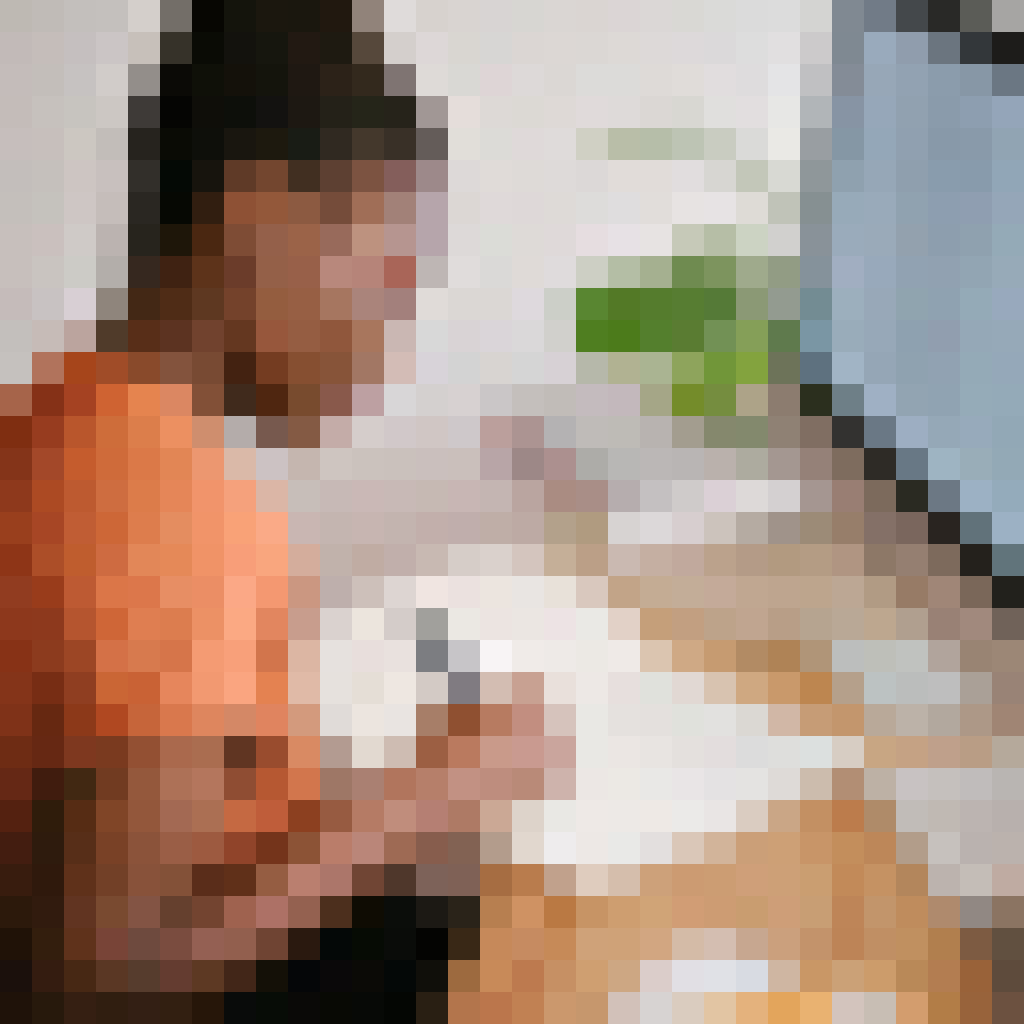
\includegraphics[width=.9\linewidth]{figures/visionscience/pexels-retha-ferguson-3059745_32pixels.jpg}
        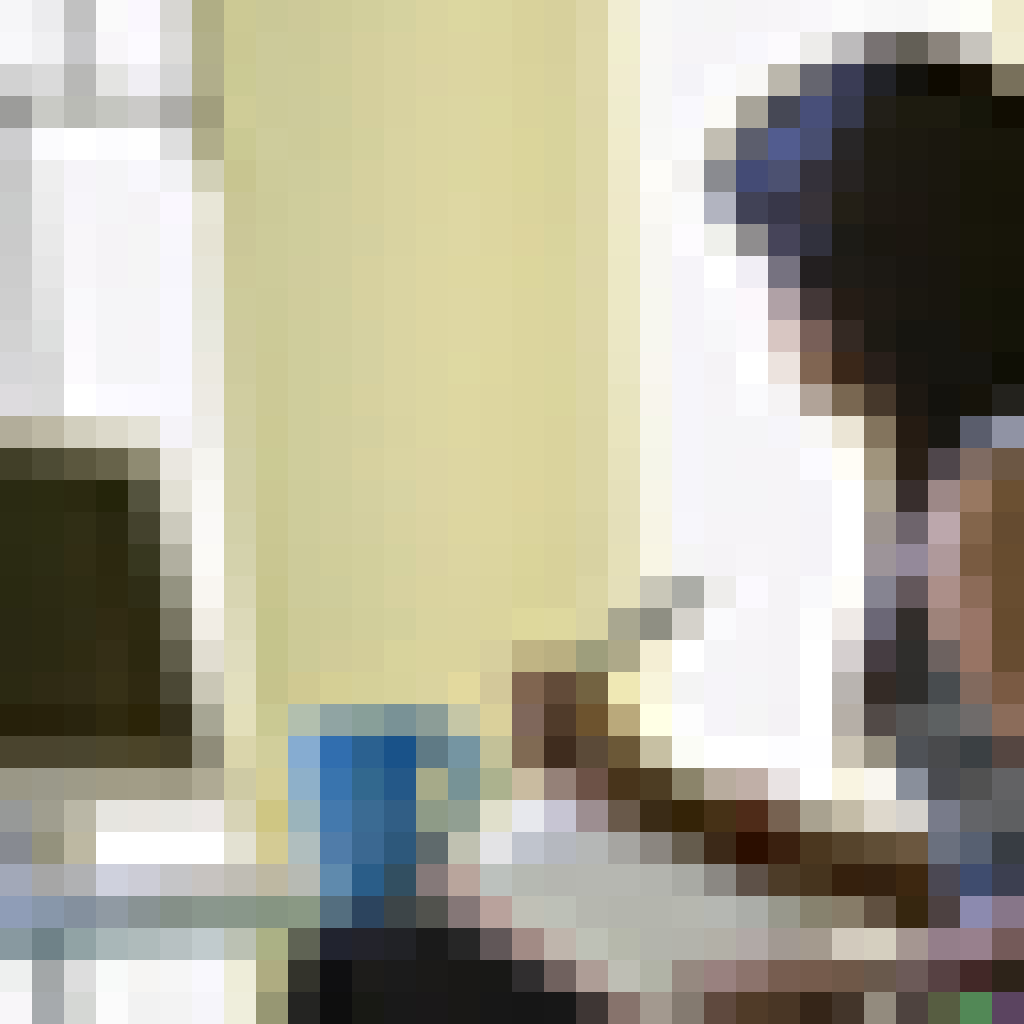
\includegraphics[width=.8\linewidth]{figures/visionscience/DALLE_32x32.png}
    }
    \caption{A tiny image with 32 $\times$ 32 color pixels. Despite the very low resolution, we can still recognize most of its content. {\em Source}: Original image created with Dall-E, and downsampled with Photoshop.}
    \label{fig:pexels-retha-ferguson}
\end{figure}
% Finally not used: Photo by Retha Ferguson from Pexels
% Original: https://www.pexels.com/photo/woman-in-front-of-her-computer-3059745/
% https://markallenassets.blob.core.windows.net/communitycare/2020/11/edit.Retha-Ferguson-from-Pexels-woman-in-front-of-her-computer-3059745.png
% we use instead photo generated with Dall-E


\marginnote{
    Same image as in \fig{\ref{fig:pexels-retha-ferguson}} but shown small.
    \\[6pt]
    \centerline{
        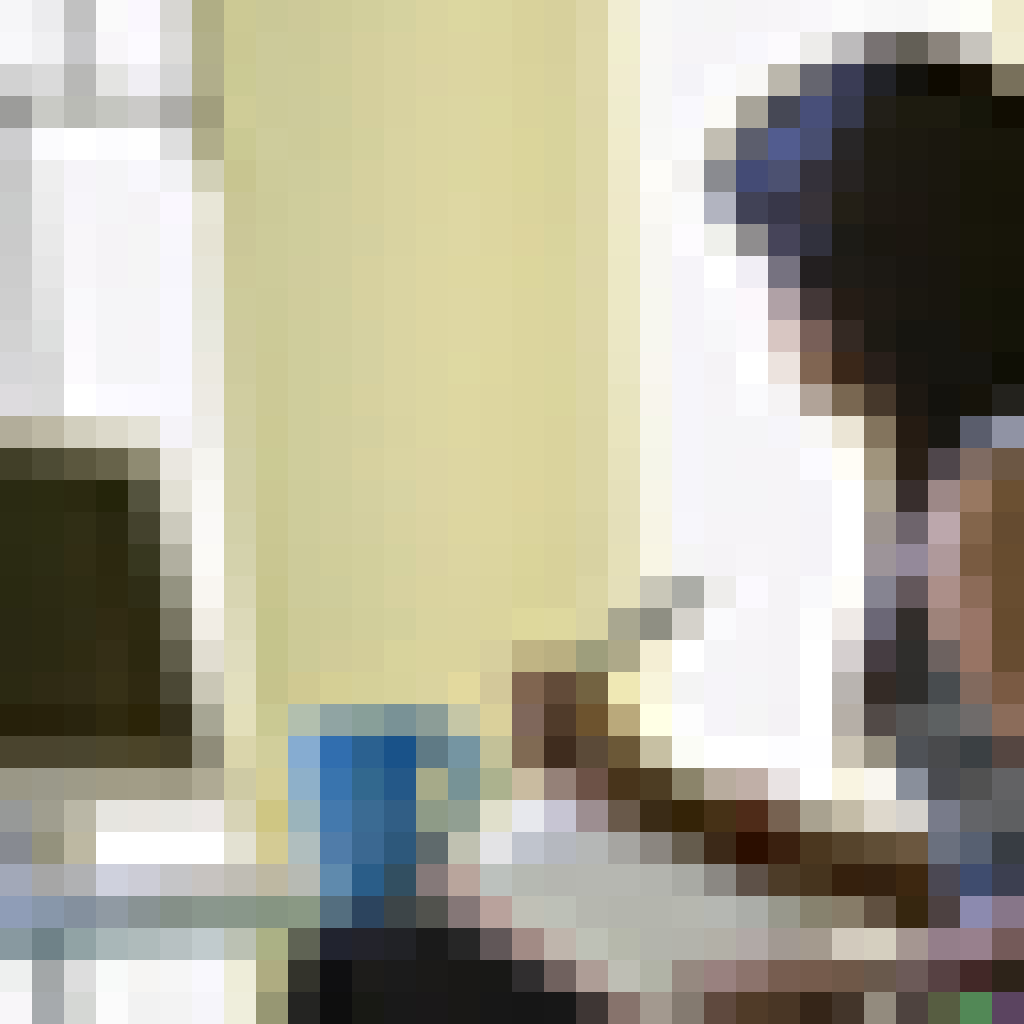
\includegraphics[width=.20\linewidth]{figures/visionscience/DALLE_32x32.png}}
    \\[6pt]
    Reducing the size helps better recognizing the objects despite containing the same visual information.
}[-3in]

Recognition of the meaning of that pixel can not come just from the intensity of that pixel or the few pixels nearby. There are way too many possible situations in which different objects in the world could map to a similar set of pixel intensities. Instead, is the whole image and the context of the pen that provides the necessary information to recognize the pen. Taken in isolation, those pixels are impossible to recognize. Here we show, from left to right, the hand, the pen, and the blue mug.


\begin{figure}[h!]
    \centerline{
        
\includegraphics[width=.17\linewidth]{figures/visionscience/dalle_hand.png}
        ~
        
\includegraphics[width=.34\linewidth]{figures/visionscience/dalle_mug.png}
        ~
        
\includegraphics[width=.29\linewidth]{figures/visionscience/dalle_pen.png}
        %~
        %
\includegraphics[width=.21\linewidth]{figures/visionscience/plant.png}
    }
    \caption{Small image patches from \fig{\ref{fig:pexels-retha-ferguson}} in isolation. It is difficult to recognize image patches outside their natural context.}
    %\label{fig:image_classification}
\end{figure}

%\centerline{
%
\includegraphics[width=.15\linewidth]{figures/visionscience/pexels-retha-ferguson-3059745_32blur.jpg}
%}


\marginnote{What is the minimum number of pixels needed to form a recognizable image? The answer depends on the image. It is possible to create visually recognizable images with very few pixels \cite{torralba_2009}.}


\section{The More You Look, the More You See}
%{\bf The more you look, the more you see.} 
Visual perception cannot be formulated as a simple input-output function over predefined domains. Vision is a dynamical system, even when looking at a static image. The longer you look at an image, the more details you see and the better you understand the scene. Just look at the image shown in \fig{\ref{fig:street_in_paris}} and try to write down everything you see down to the smallest detail.

% Some useful reference: https://www.pnas.org/content/112/12/3618

% http://groups.csail.mit.edu/vision/datasets/ADE20K//ADE20K_2016_07_26/images/training/r/restaurant_patio/ADE_train_00015819.jpg
\begin{figure}[t]
    \centerline{
        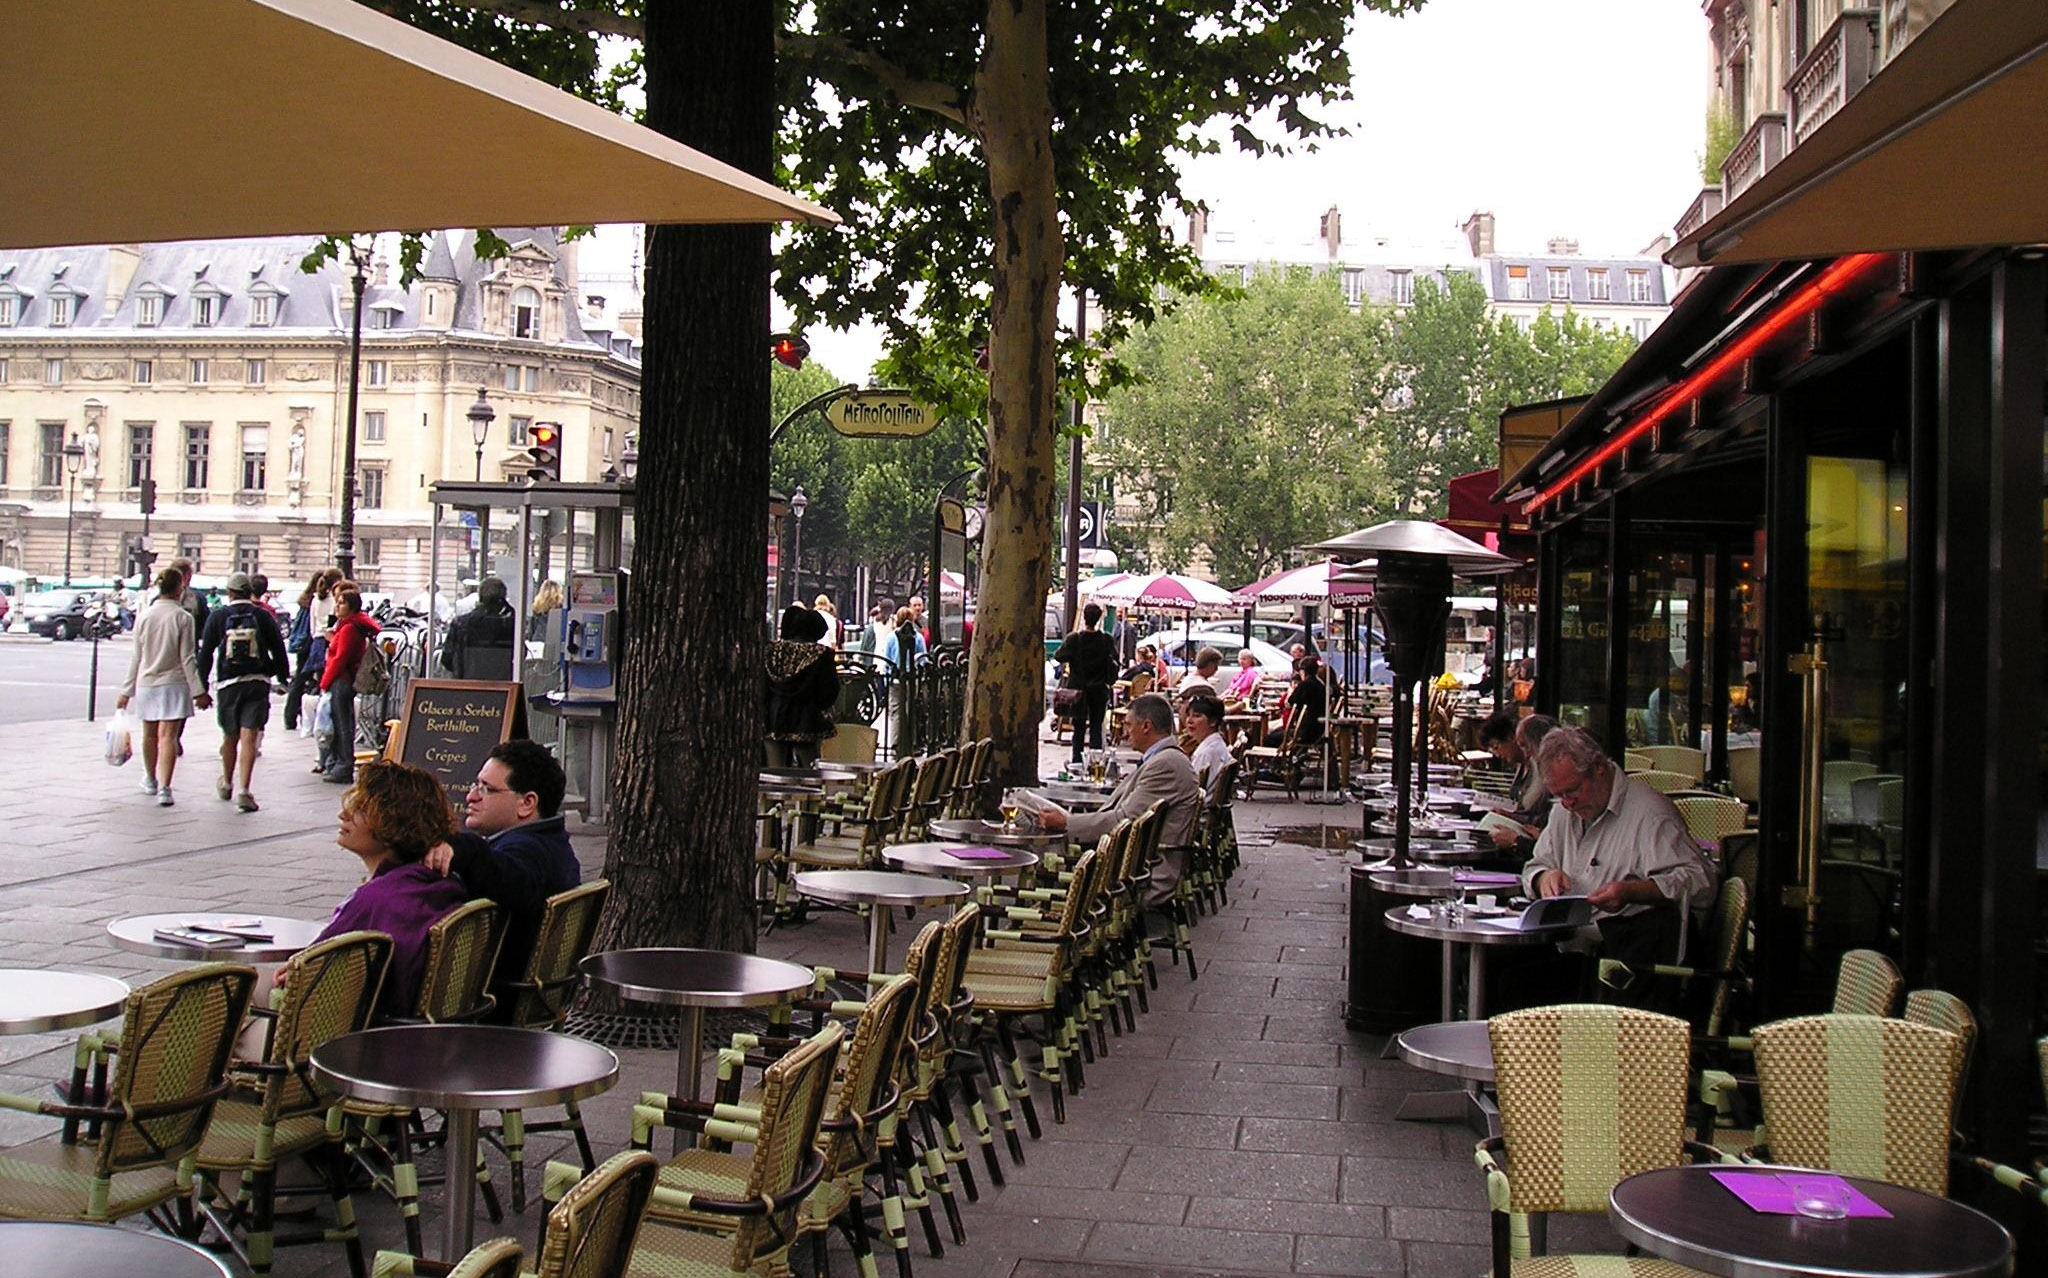
\includegraphics[width=.98\linewidth]{figures/visionscience/ADE_train_00015819_messed_small.jpg}
    }
    \caption{A street in Paris. Is everything fine in this picture?}
    \label{fig:street_in_paris}
\end{figure}
% Photo by Antonio Torralba


But this feeling of unlimited and effortless understanding of a picture is also an illusion. Do you truly understand everything you see? For instance, are you sure you can make sense of all the chair legs in \fig{\ref{fig:street_in_paris}}? In fact, this image has been manipulated so that some of legs do not correspond to any chair.

\marginnote{When solving a task, as the {\bf visual cognitive load} increases we are more likely to make judgment mistakes.
    % https://graphics.stanford.edu/papers/visual-cognitive-load/klingner_aural_vs_visual_cognitive_load.pdf
}

As you look around the image, notice that each patch you look at is actually a small photo in its own right. In fact, a big image like this contains thousands of tiny images within it (\fig{\ref{fig:tiny_images}}). A single photo can be \textit{big data}; if you chop up this photo you get a big dataset of tiny images.
A common trick in computer vision is to take a method that was developed for processing a dataset and instead apply it to the set of patches in an image, or vice versa.


\begin{figure}[t]
    \centerline{
        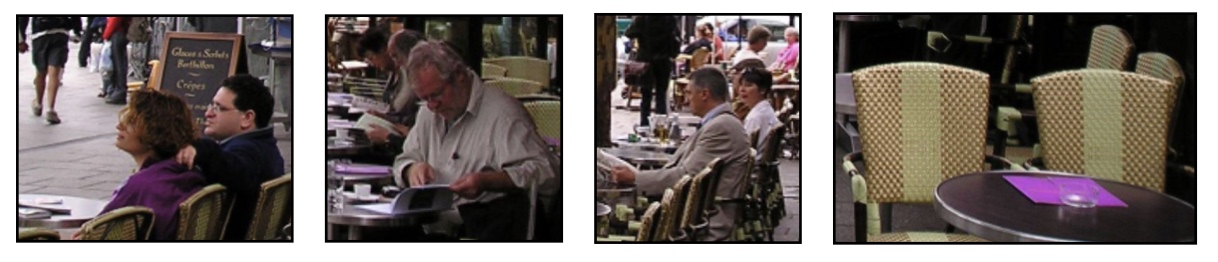
\includegraphics[width=1\linewidth]{figures/visionscience/tiny_images.jpg}
    }
    \caption{Each picture contains lots of images.}
    \label{fig:tiny_images}
\end{figure}


% \begin{center}
%     patch : image :: image : dataset
% \end{center}

\section{The Eye of the Artist}

Learning to paint is a great way of learning to see. You start from a white piece of canvas and a finite set of acrylic paints, and your goal is to paint an object that should look real, with shadows, 3D shape, and reflections. What mixtures of paint and what strokes can accomplish that? Artists learn to see the world not by what it represents, but as why it looks the way it does.

The following sequence (\fig{\ref{fig:agata_painting}}), painted by Agata Lapedriza, shows different steps in the painting process of a strawberry. Layer after layer, the artist replicates the light that will fool your eye into seeing a strawberry instead of acrylic paint. It is interesting to see that the realism does not increase monotonically as the painting progresses. For instance, from step 3 to 4, the right side of the strawberry has lost realism. However, those new strokes will become the shading that will make the strawberry pop out from the canvas.

\begin{figure}
    \centerline{
        ~1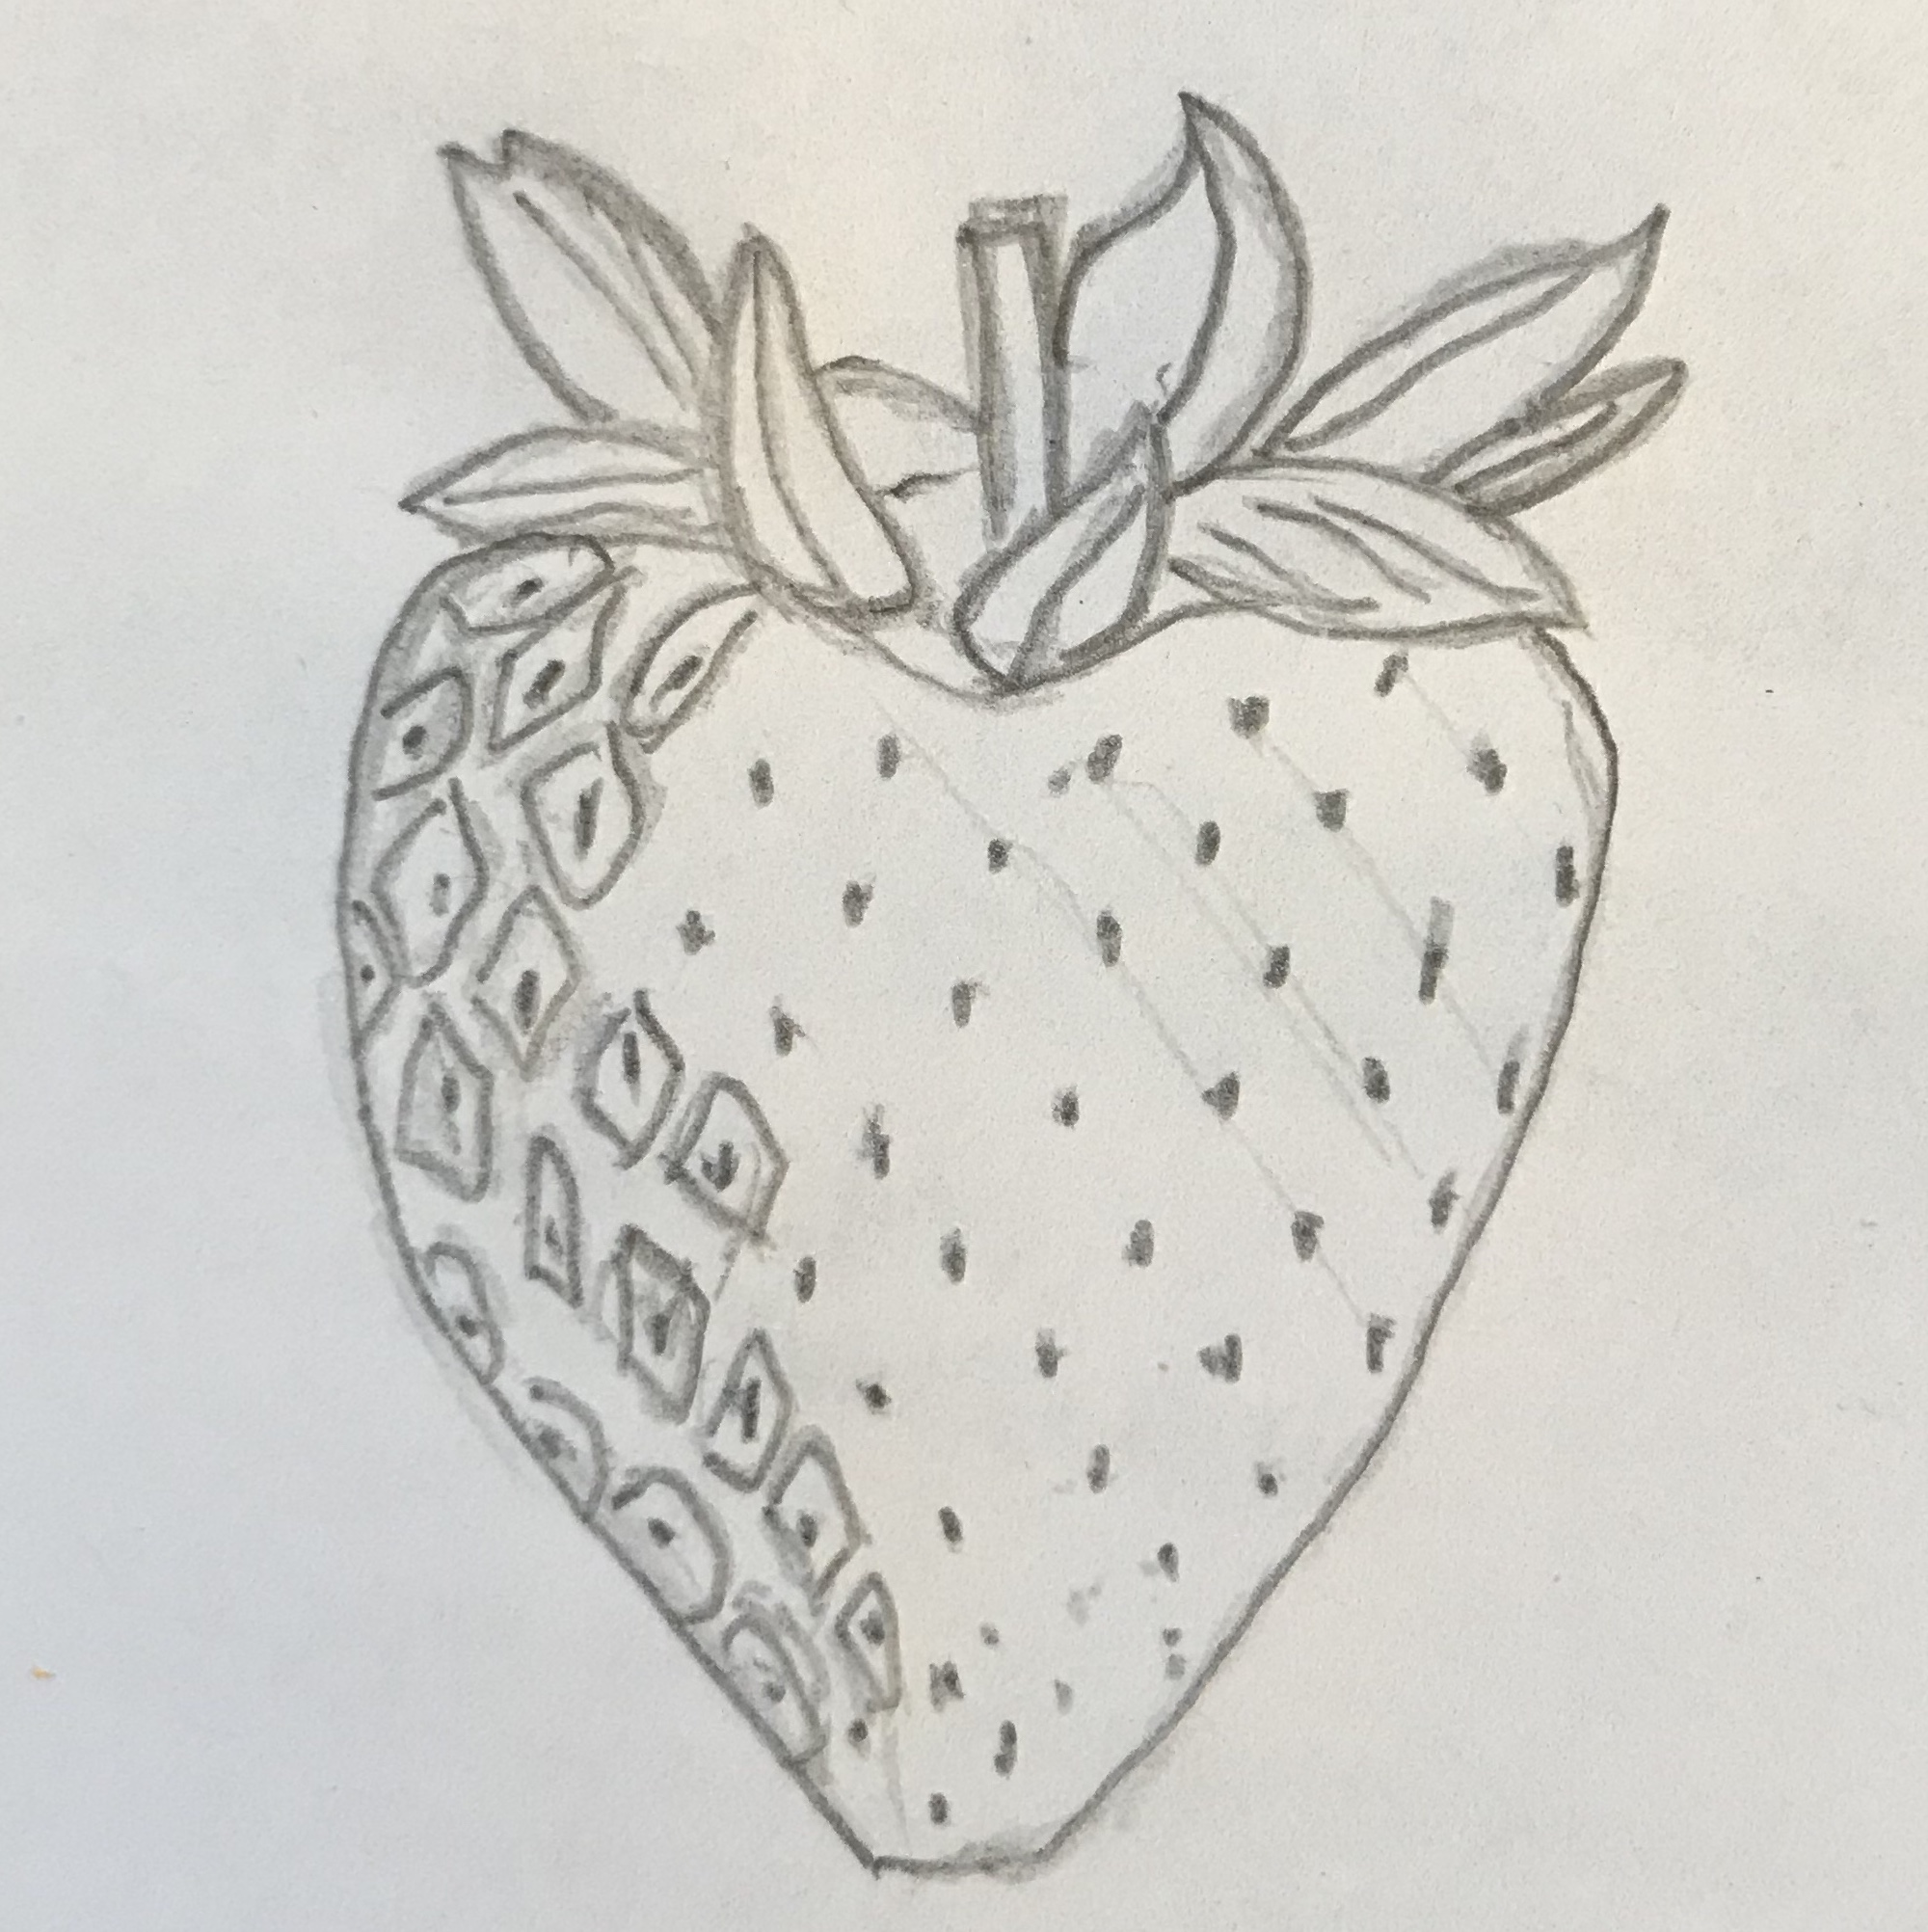
\includegraphics[width=.22\linewidth]{figures/visionscience/fresa_1.jpg}
        2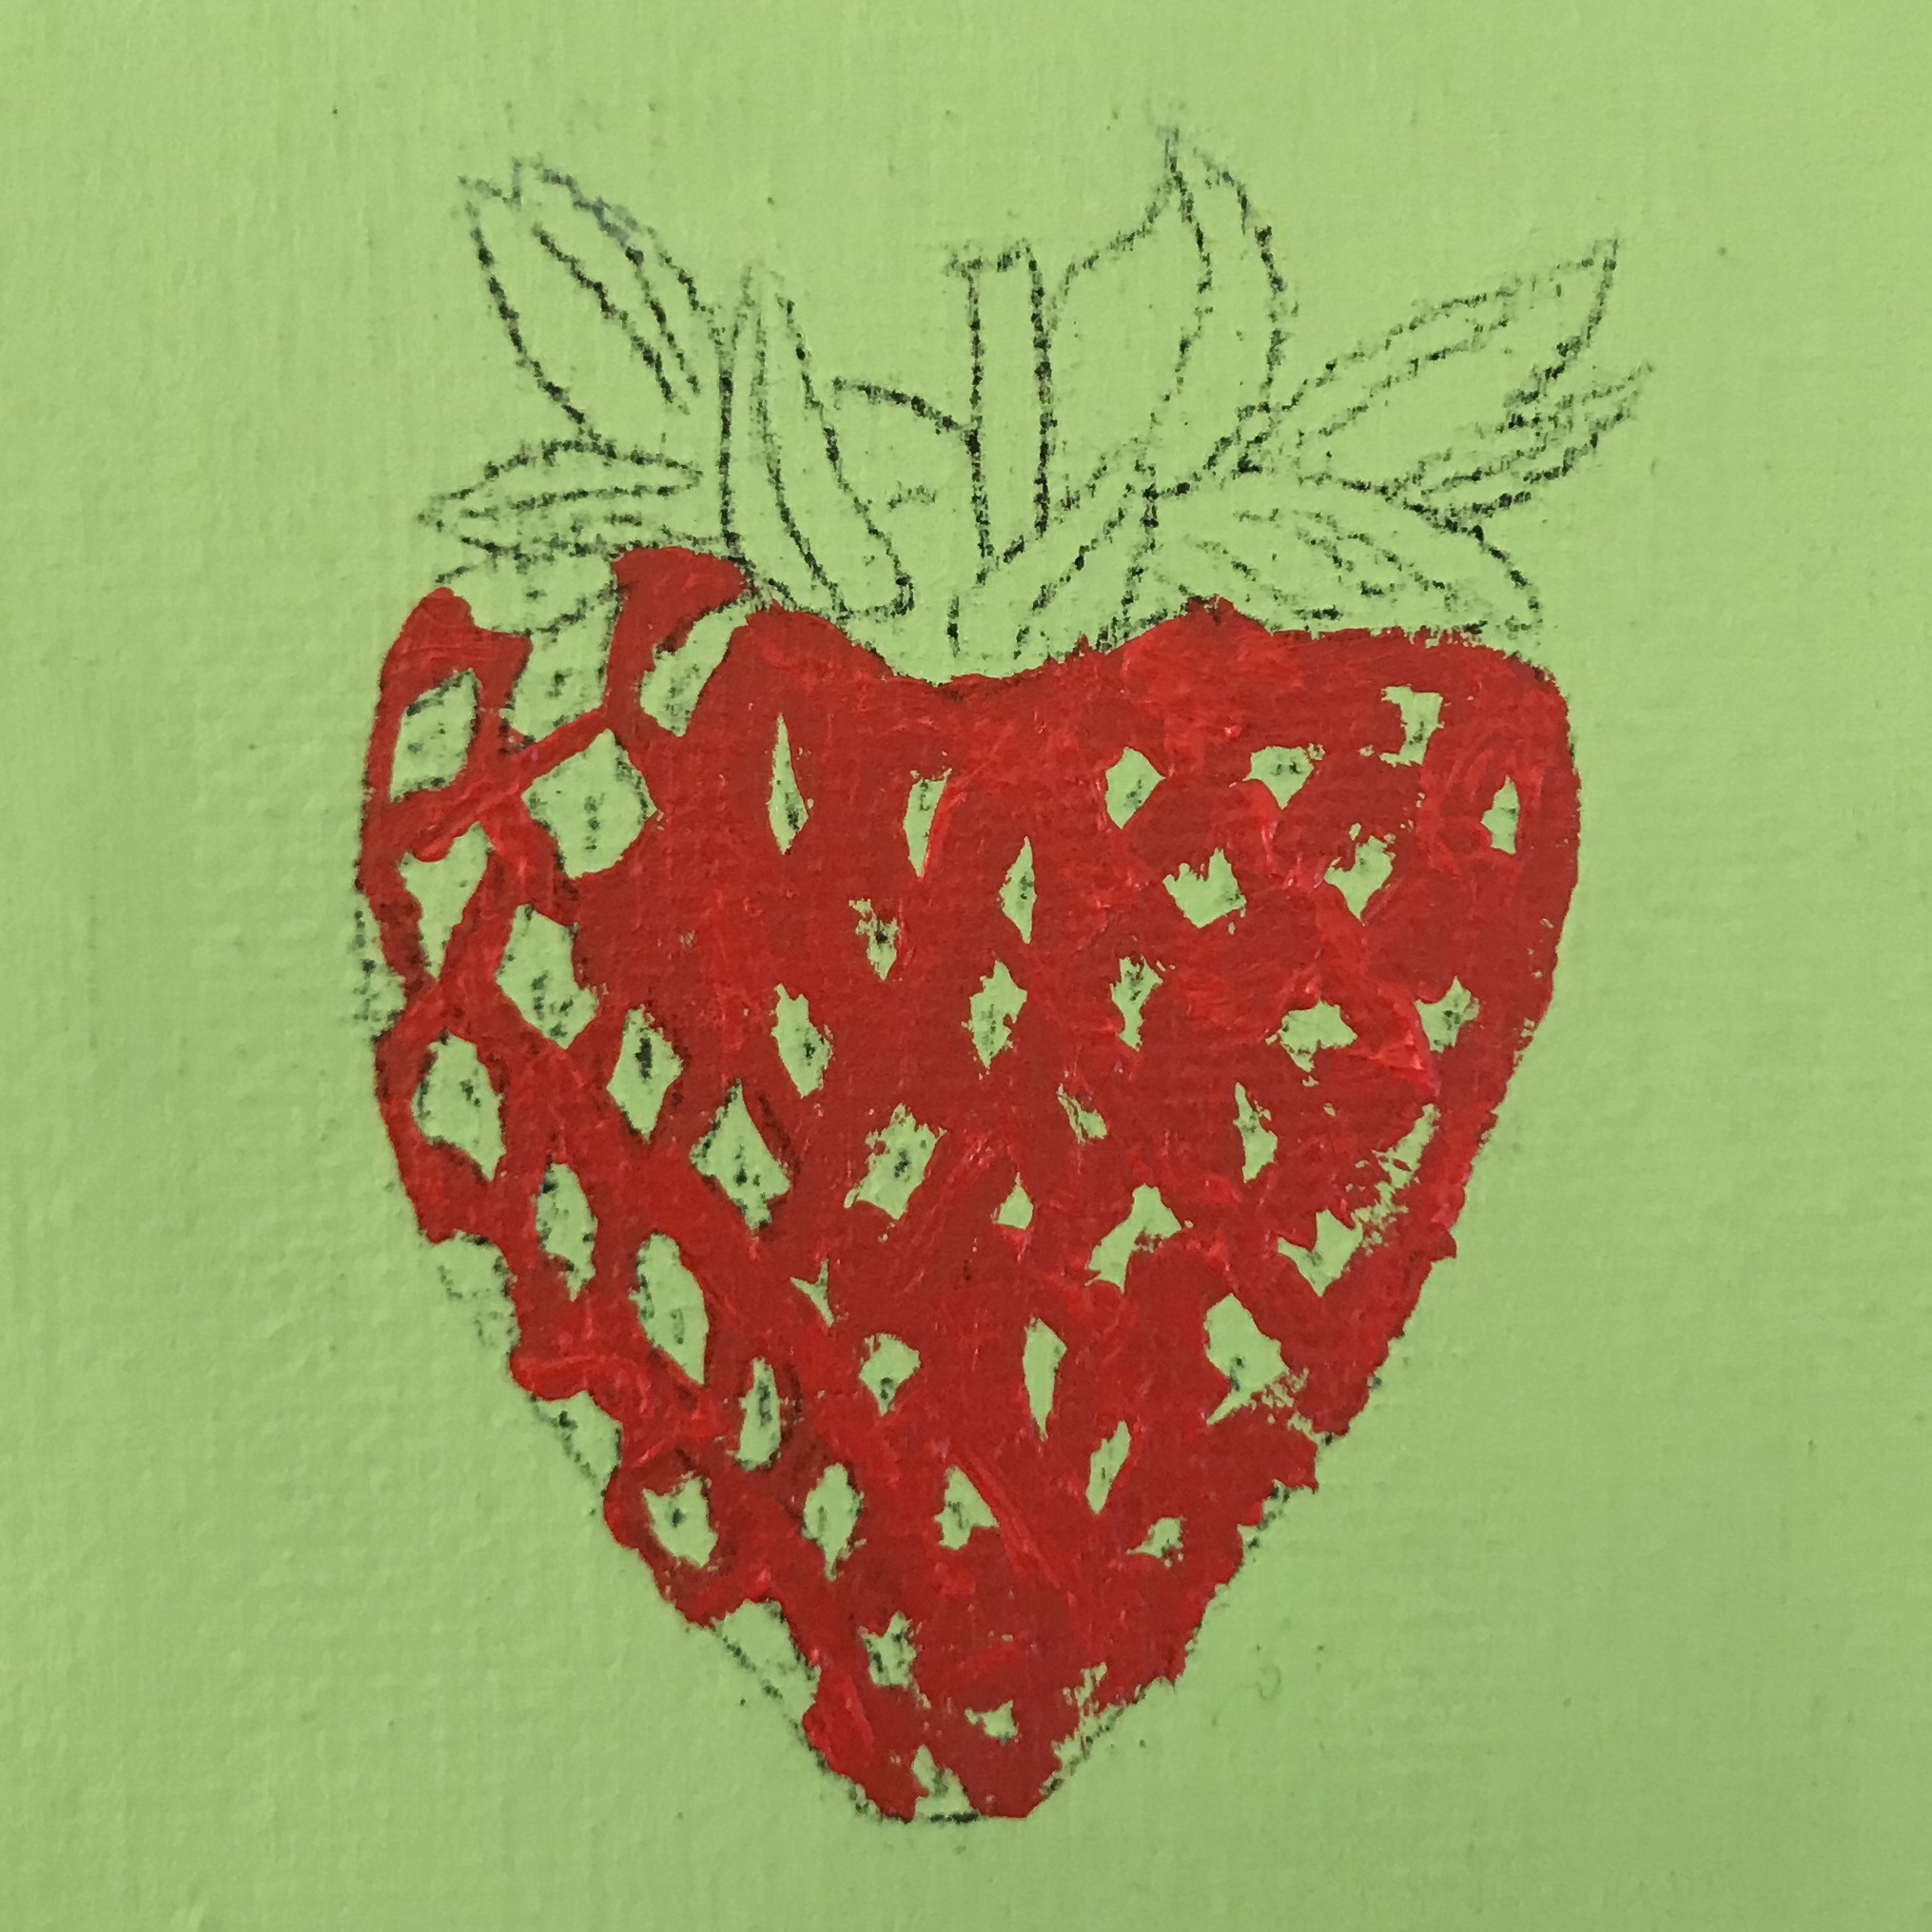
\includegraphics[width=.22\linewidth]{figures/visionscience/fresa_2.jpg}
        3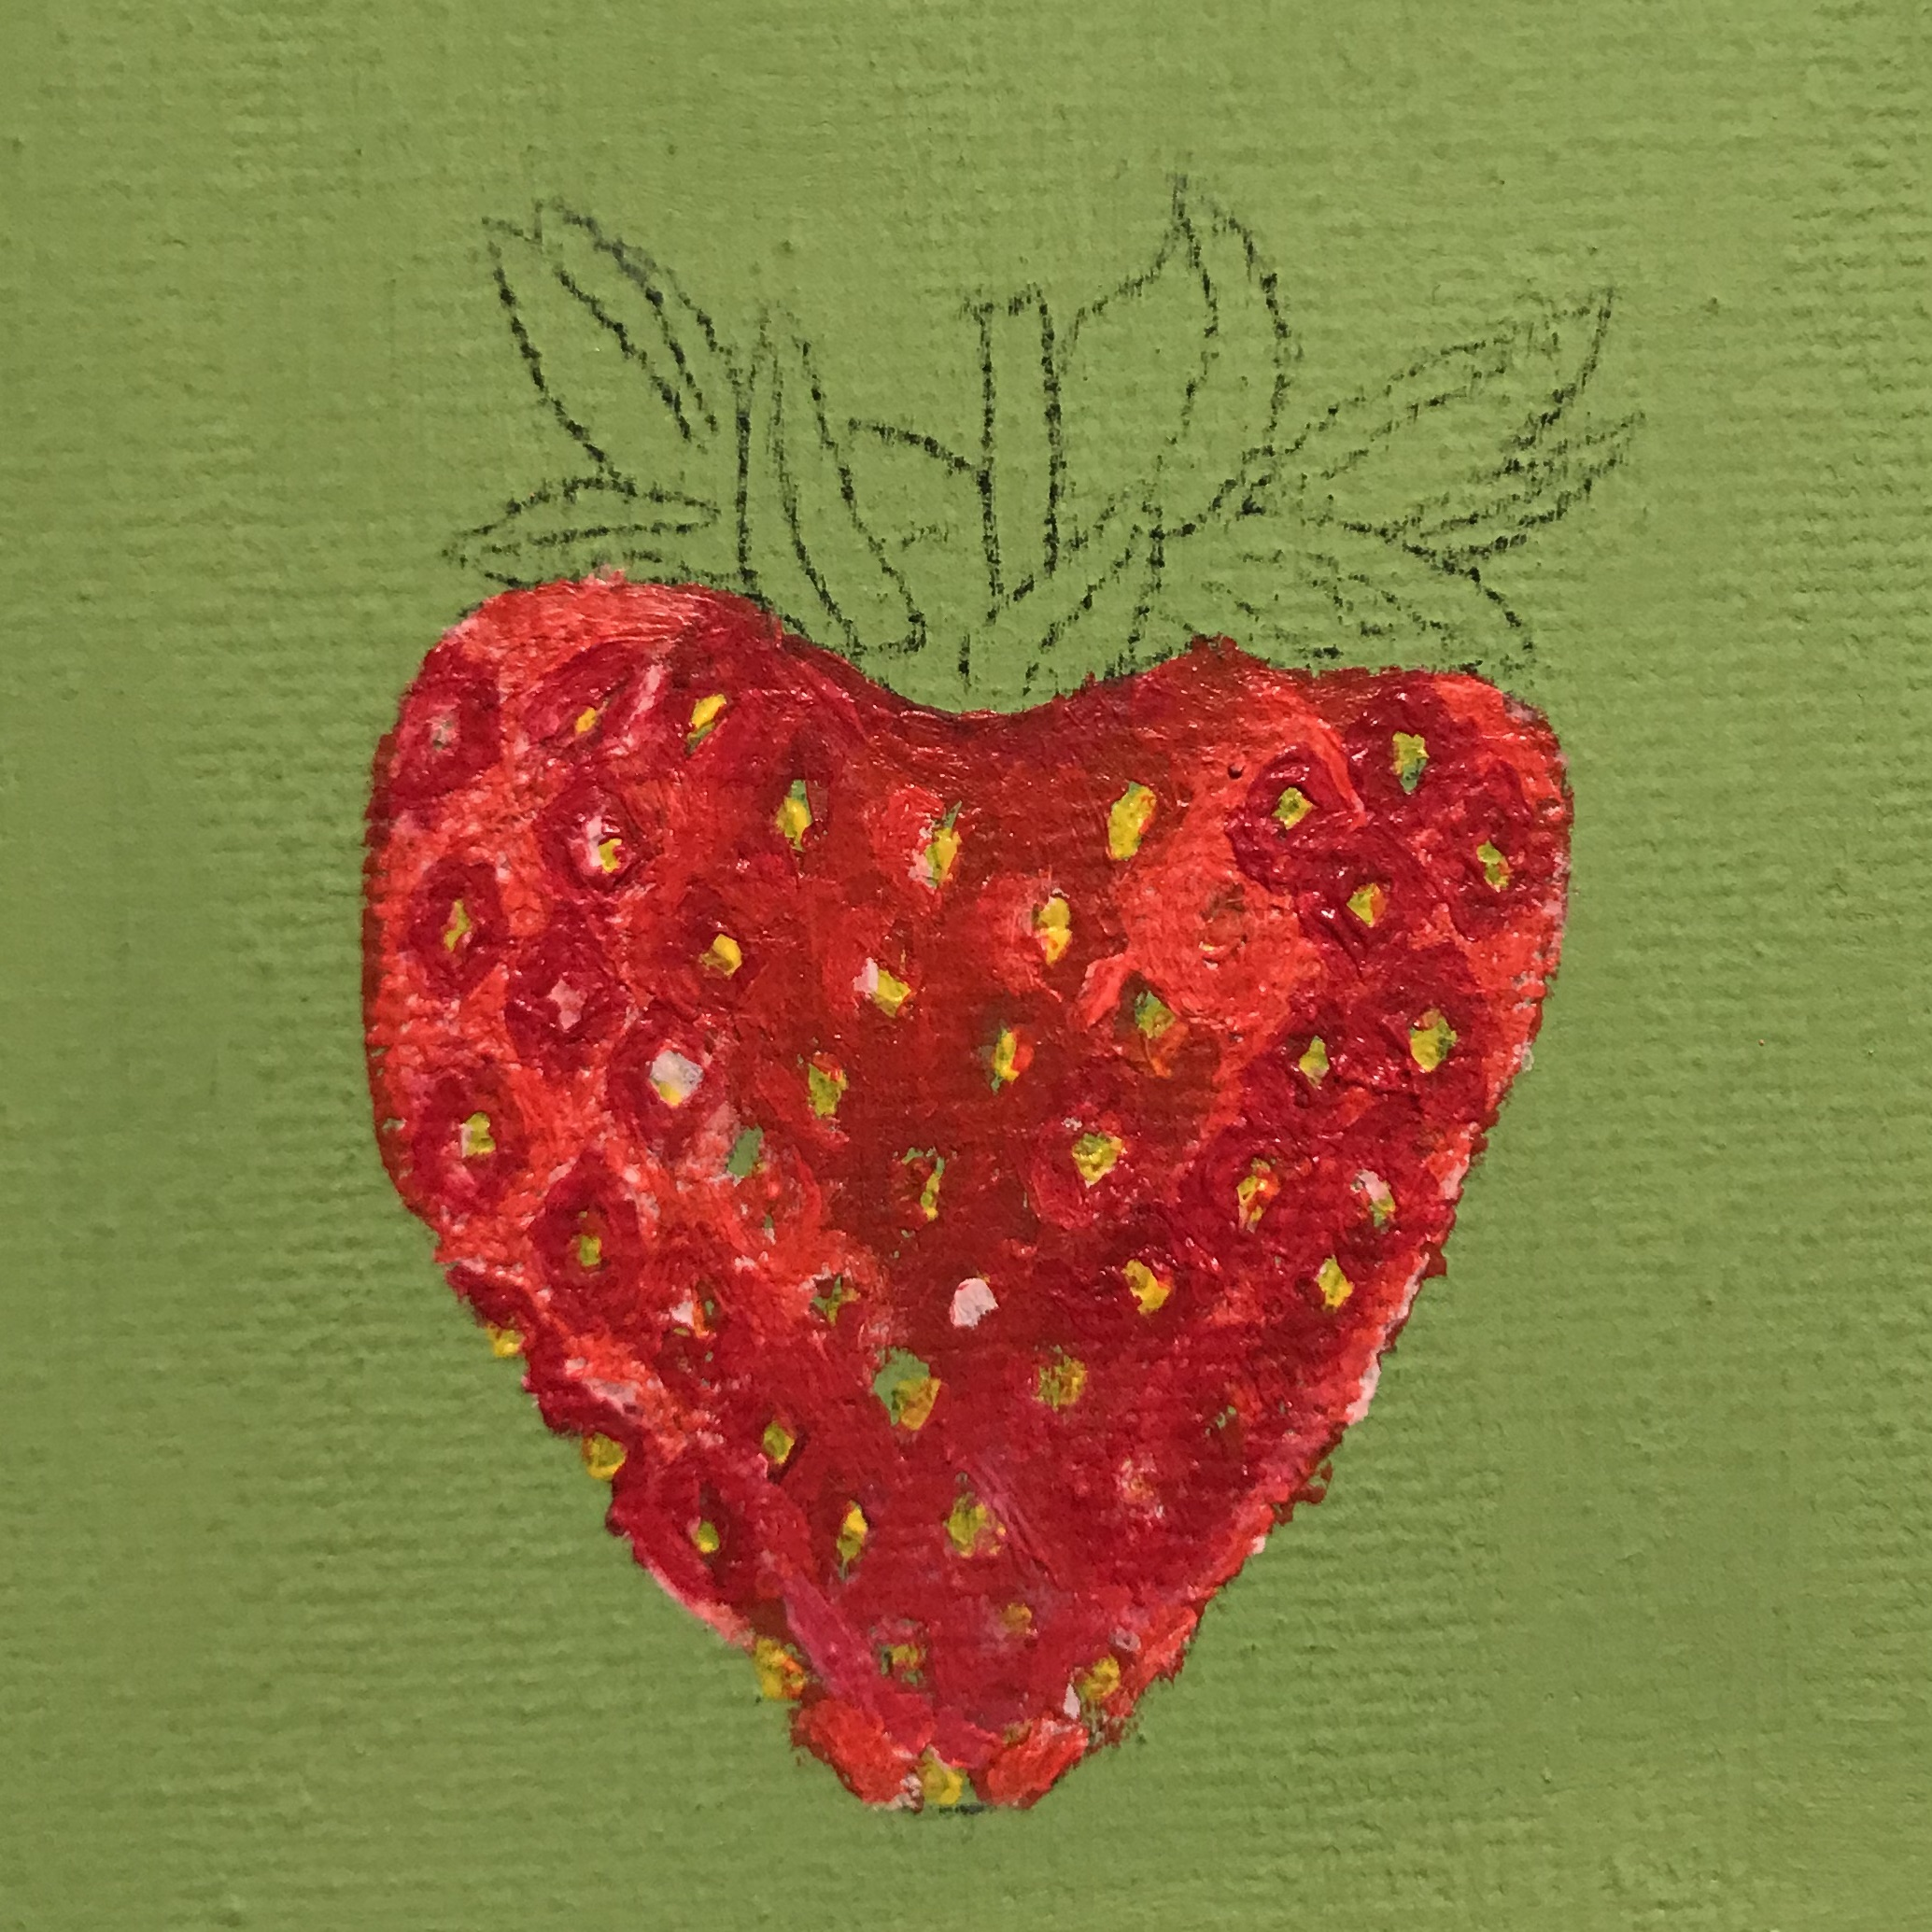
\includegraphics[width=.22\linewidth]{figures/visionscience/fresa_3.jpg}
        4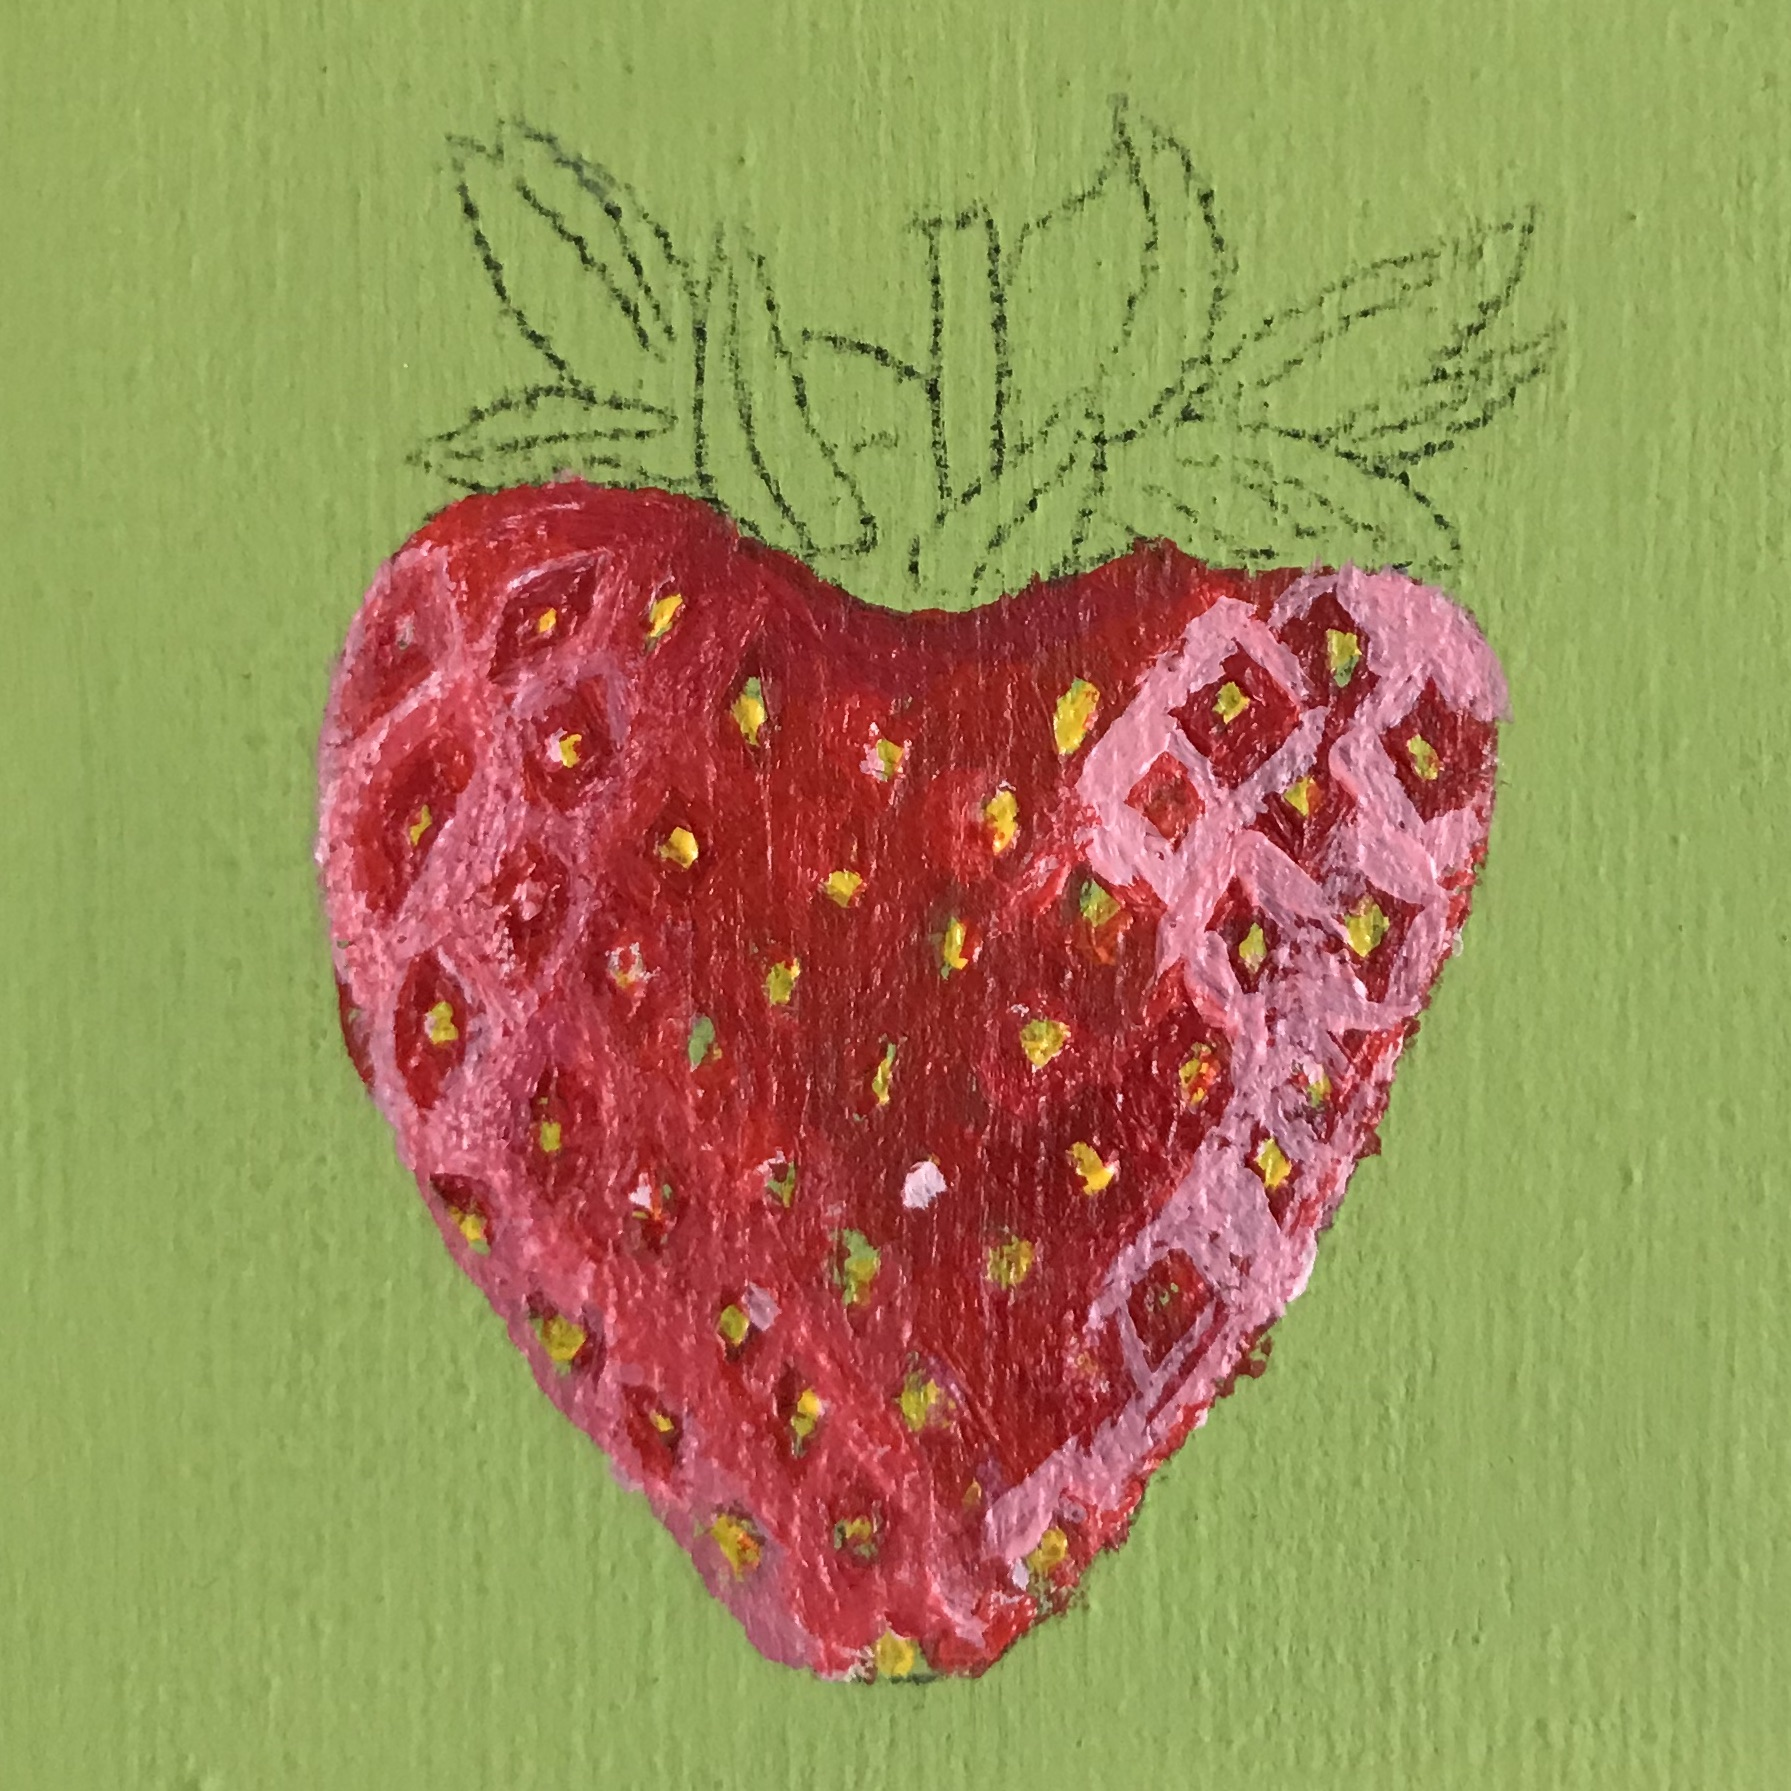
\includegraphics[width=.22\linewidth]{figures/visionscience/fresa_4.jpg}
    }
    \centerline{
        ~~5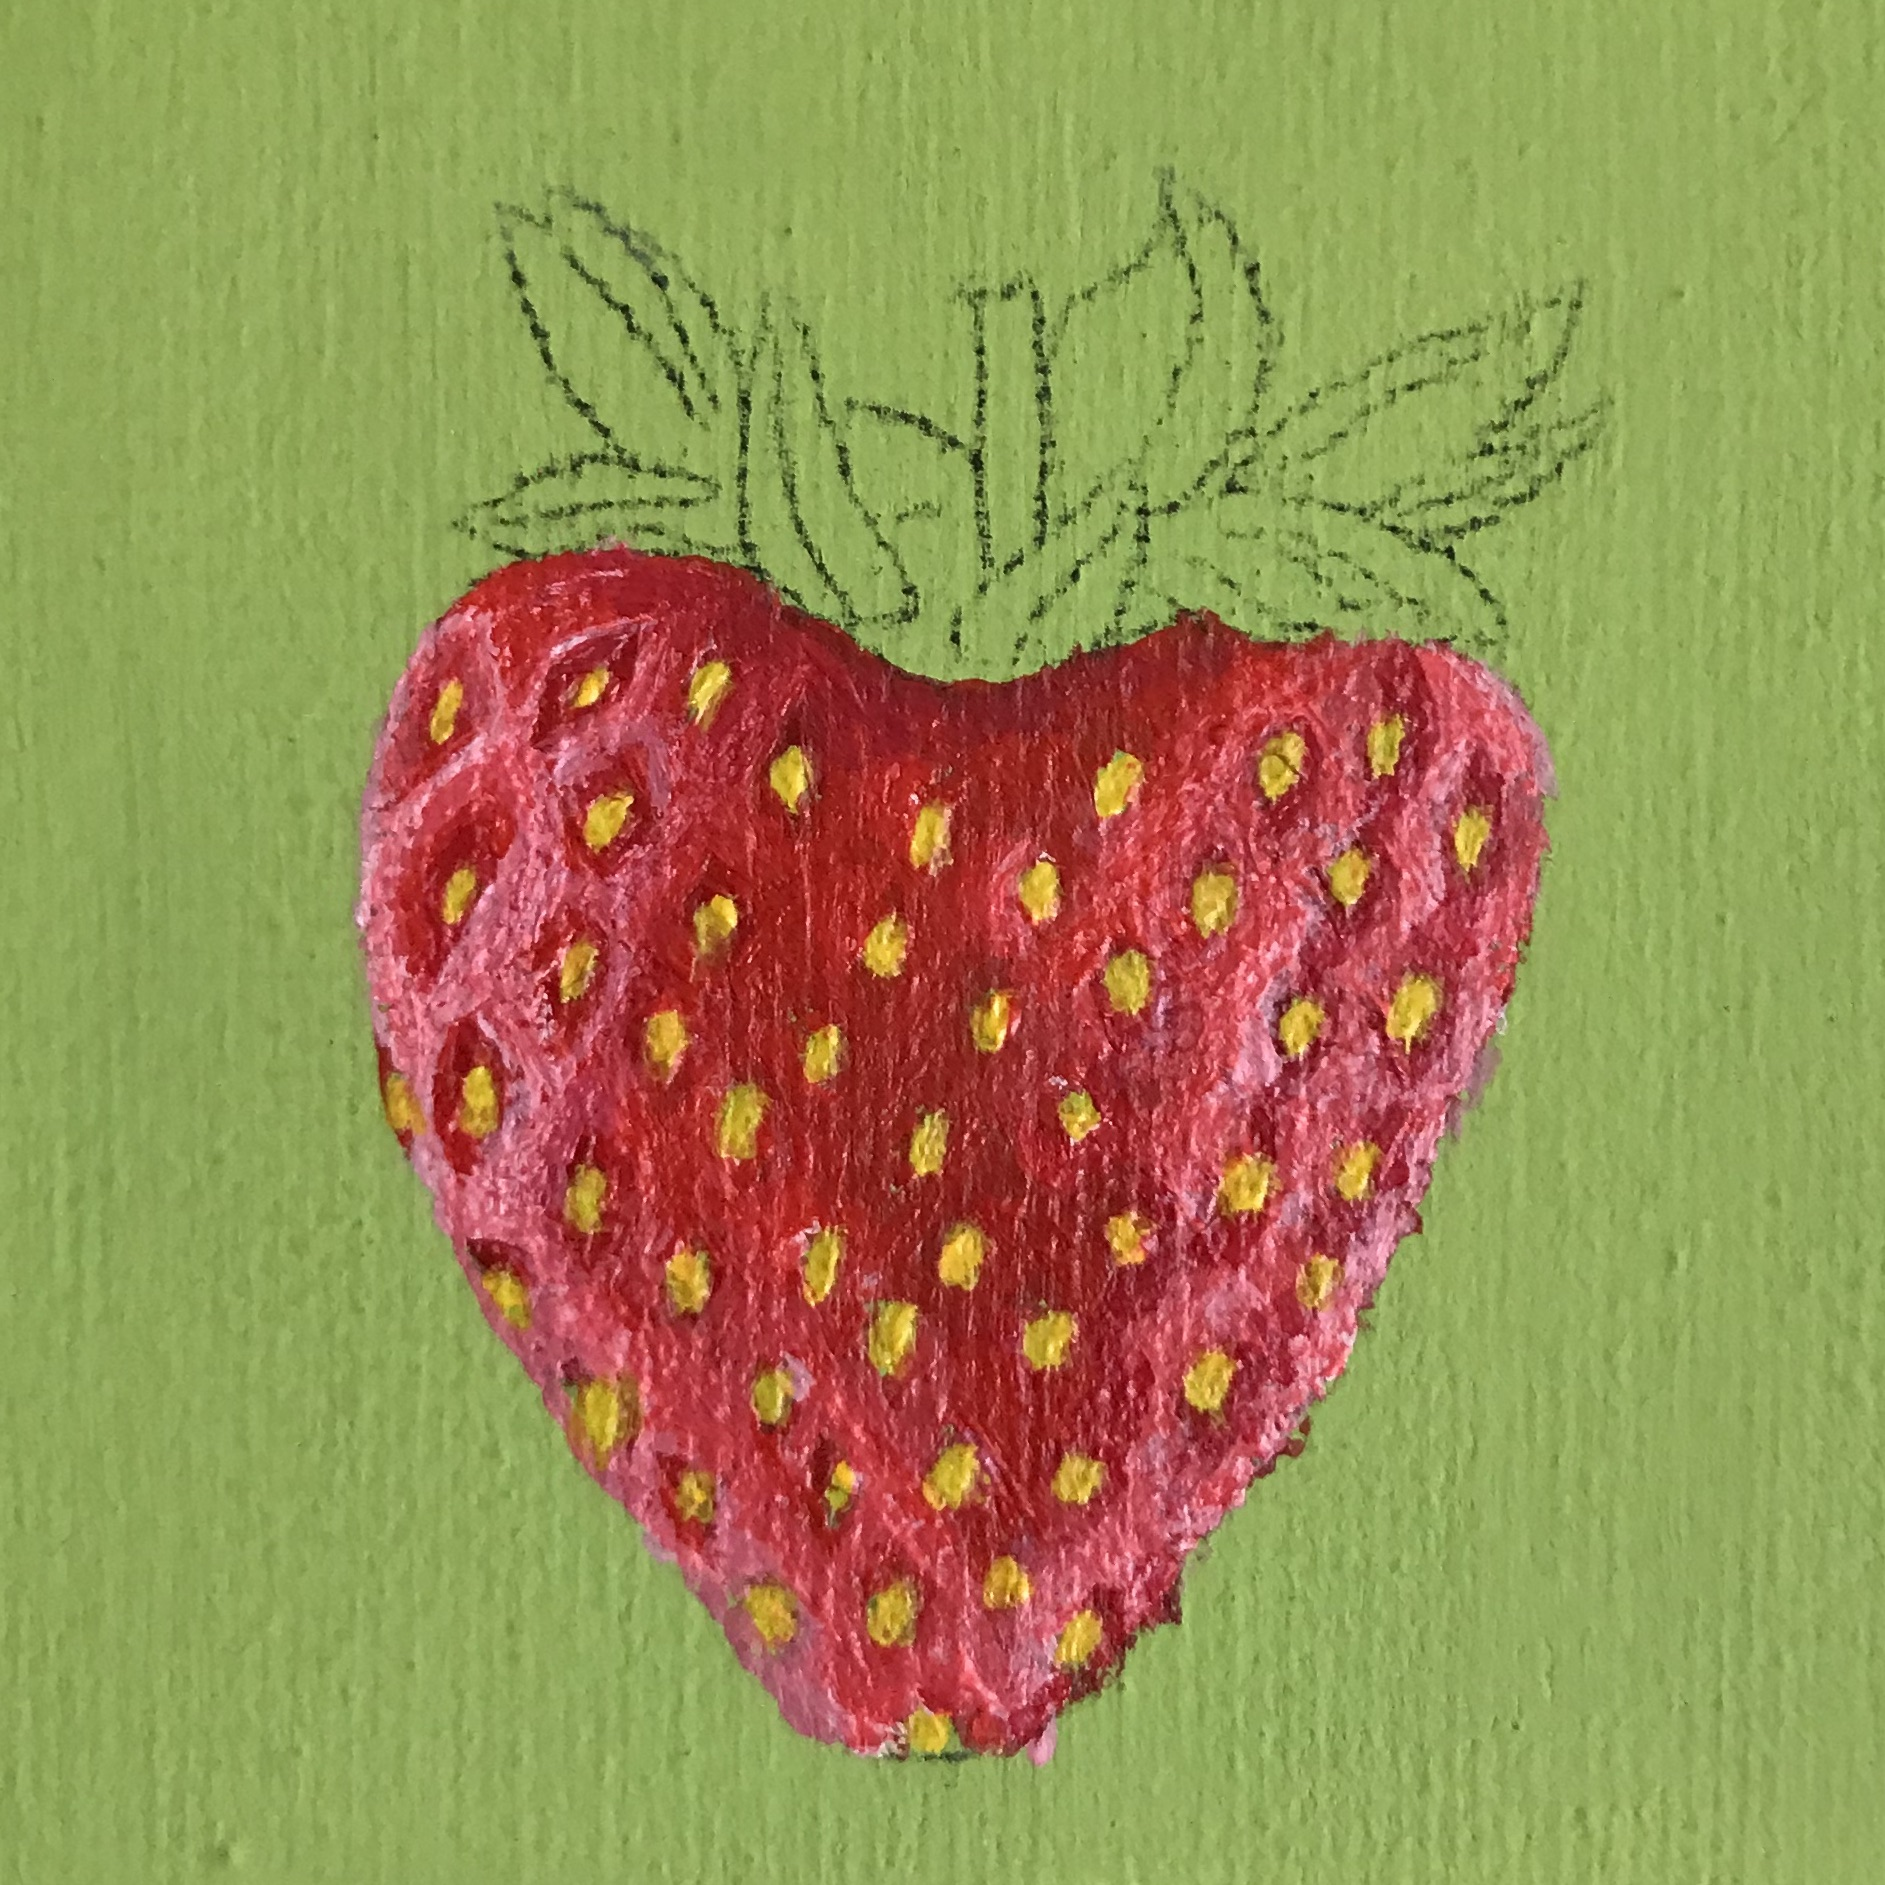
\includegraphics[width=.22\linewidth]{figures/visionscience/fresa_5.jpg}
        6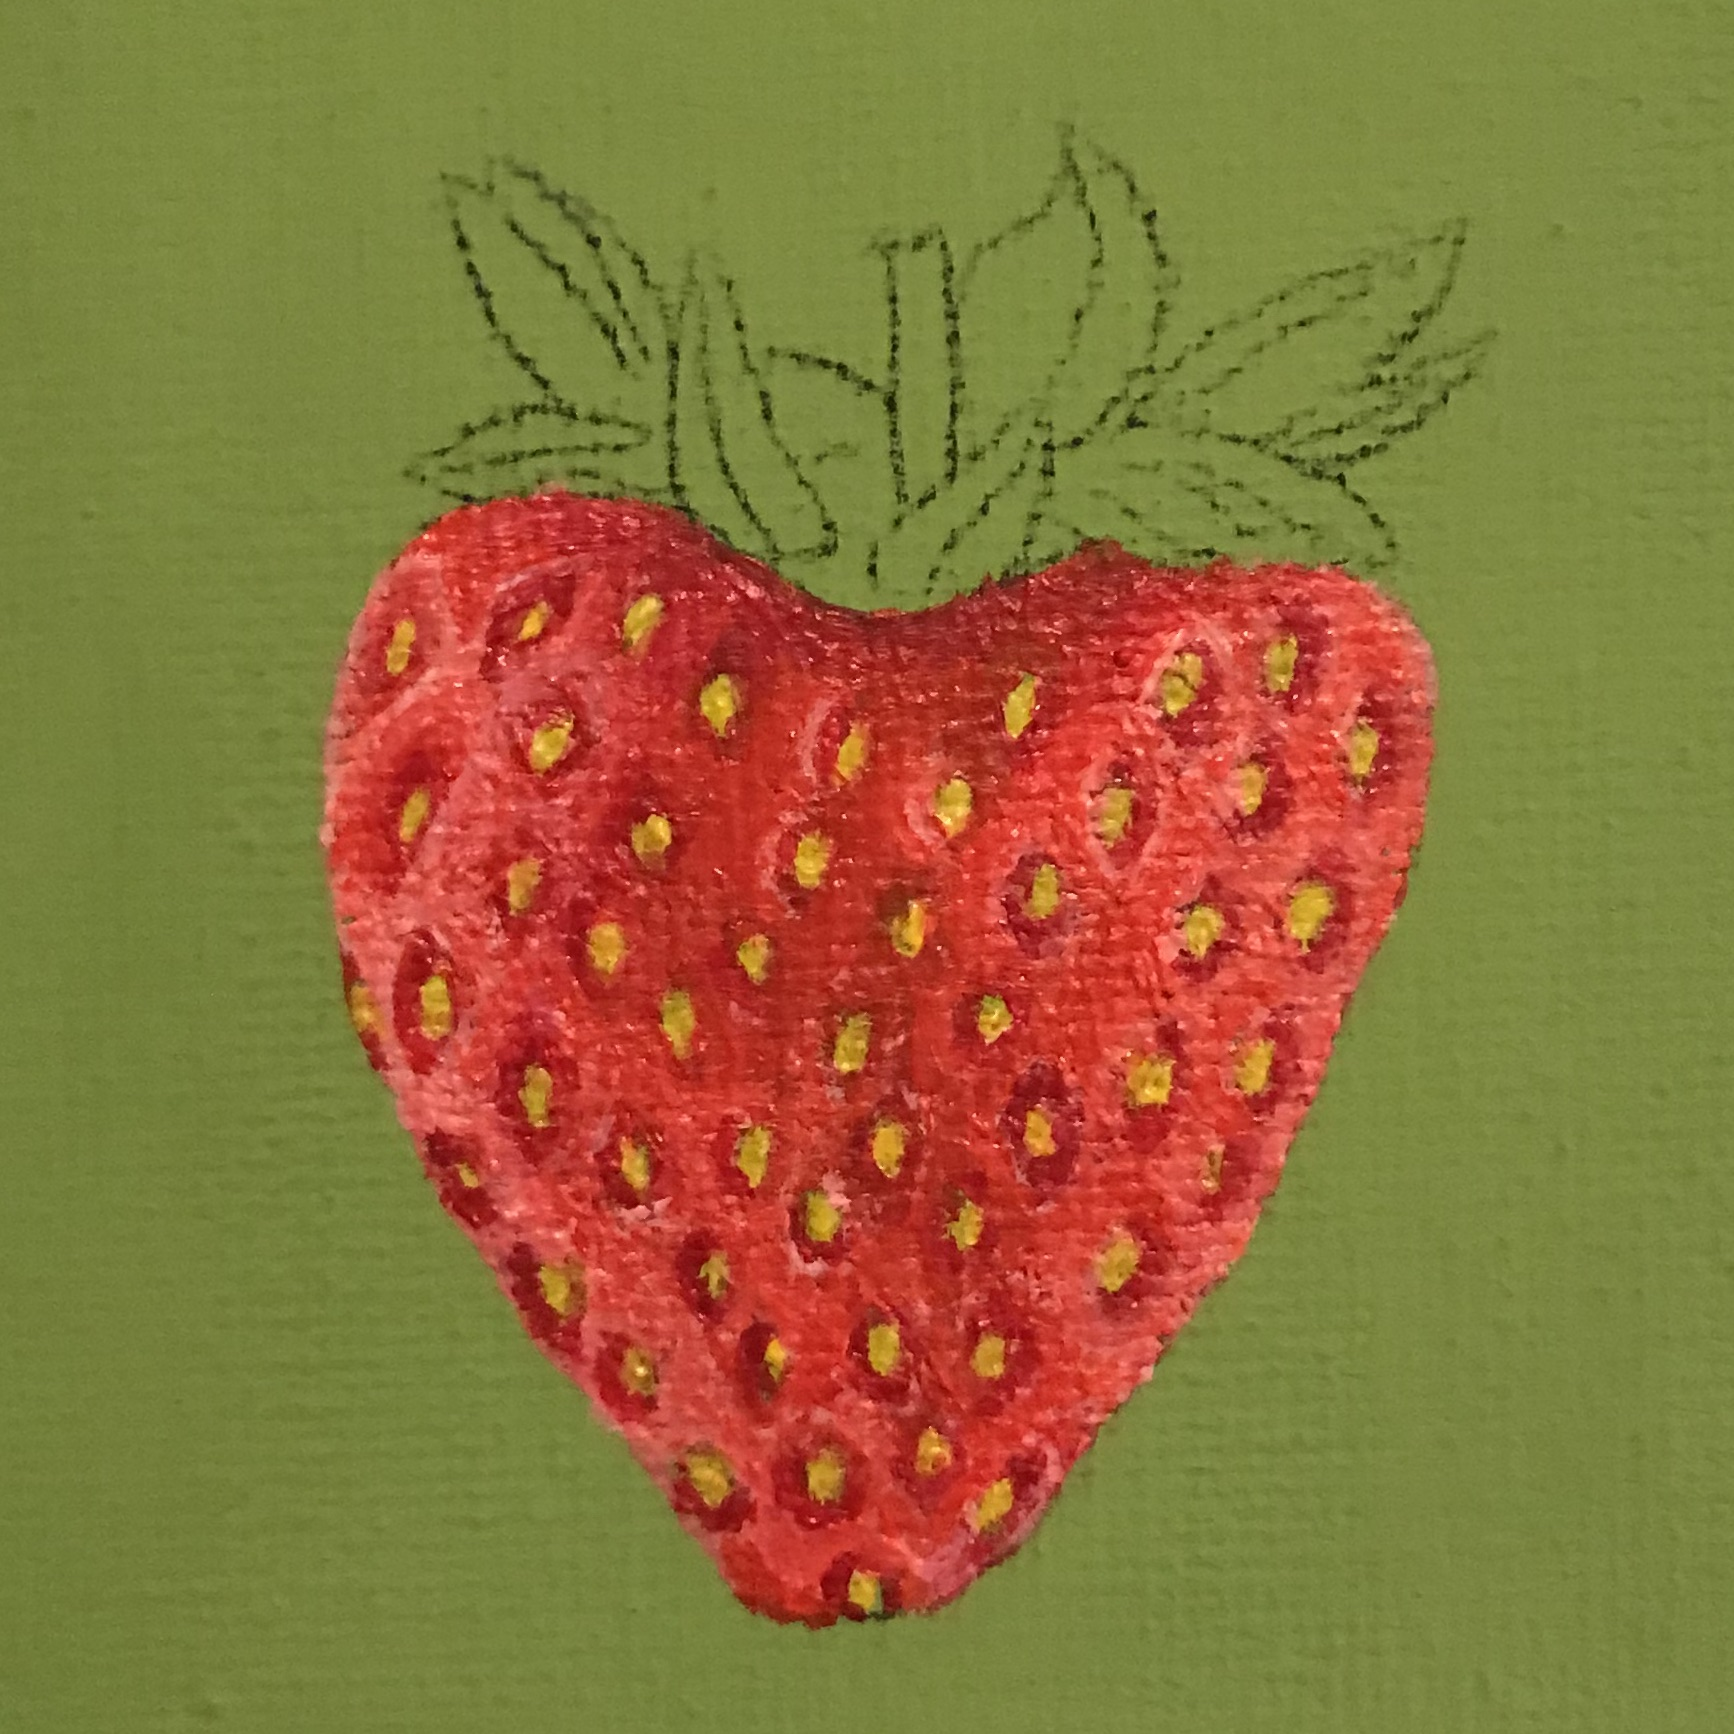
\includegraphics[width=.22\linewidth]{figures/visionscience/fresa_6.jpg}
        7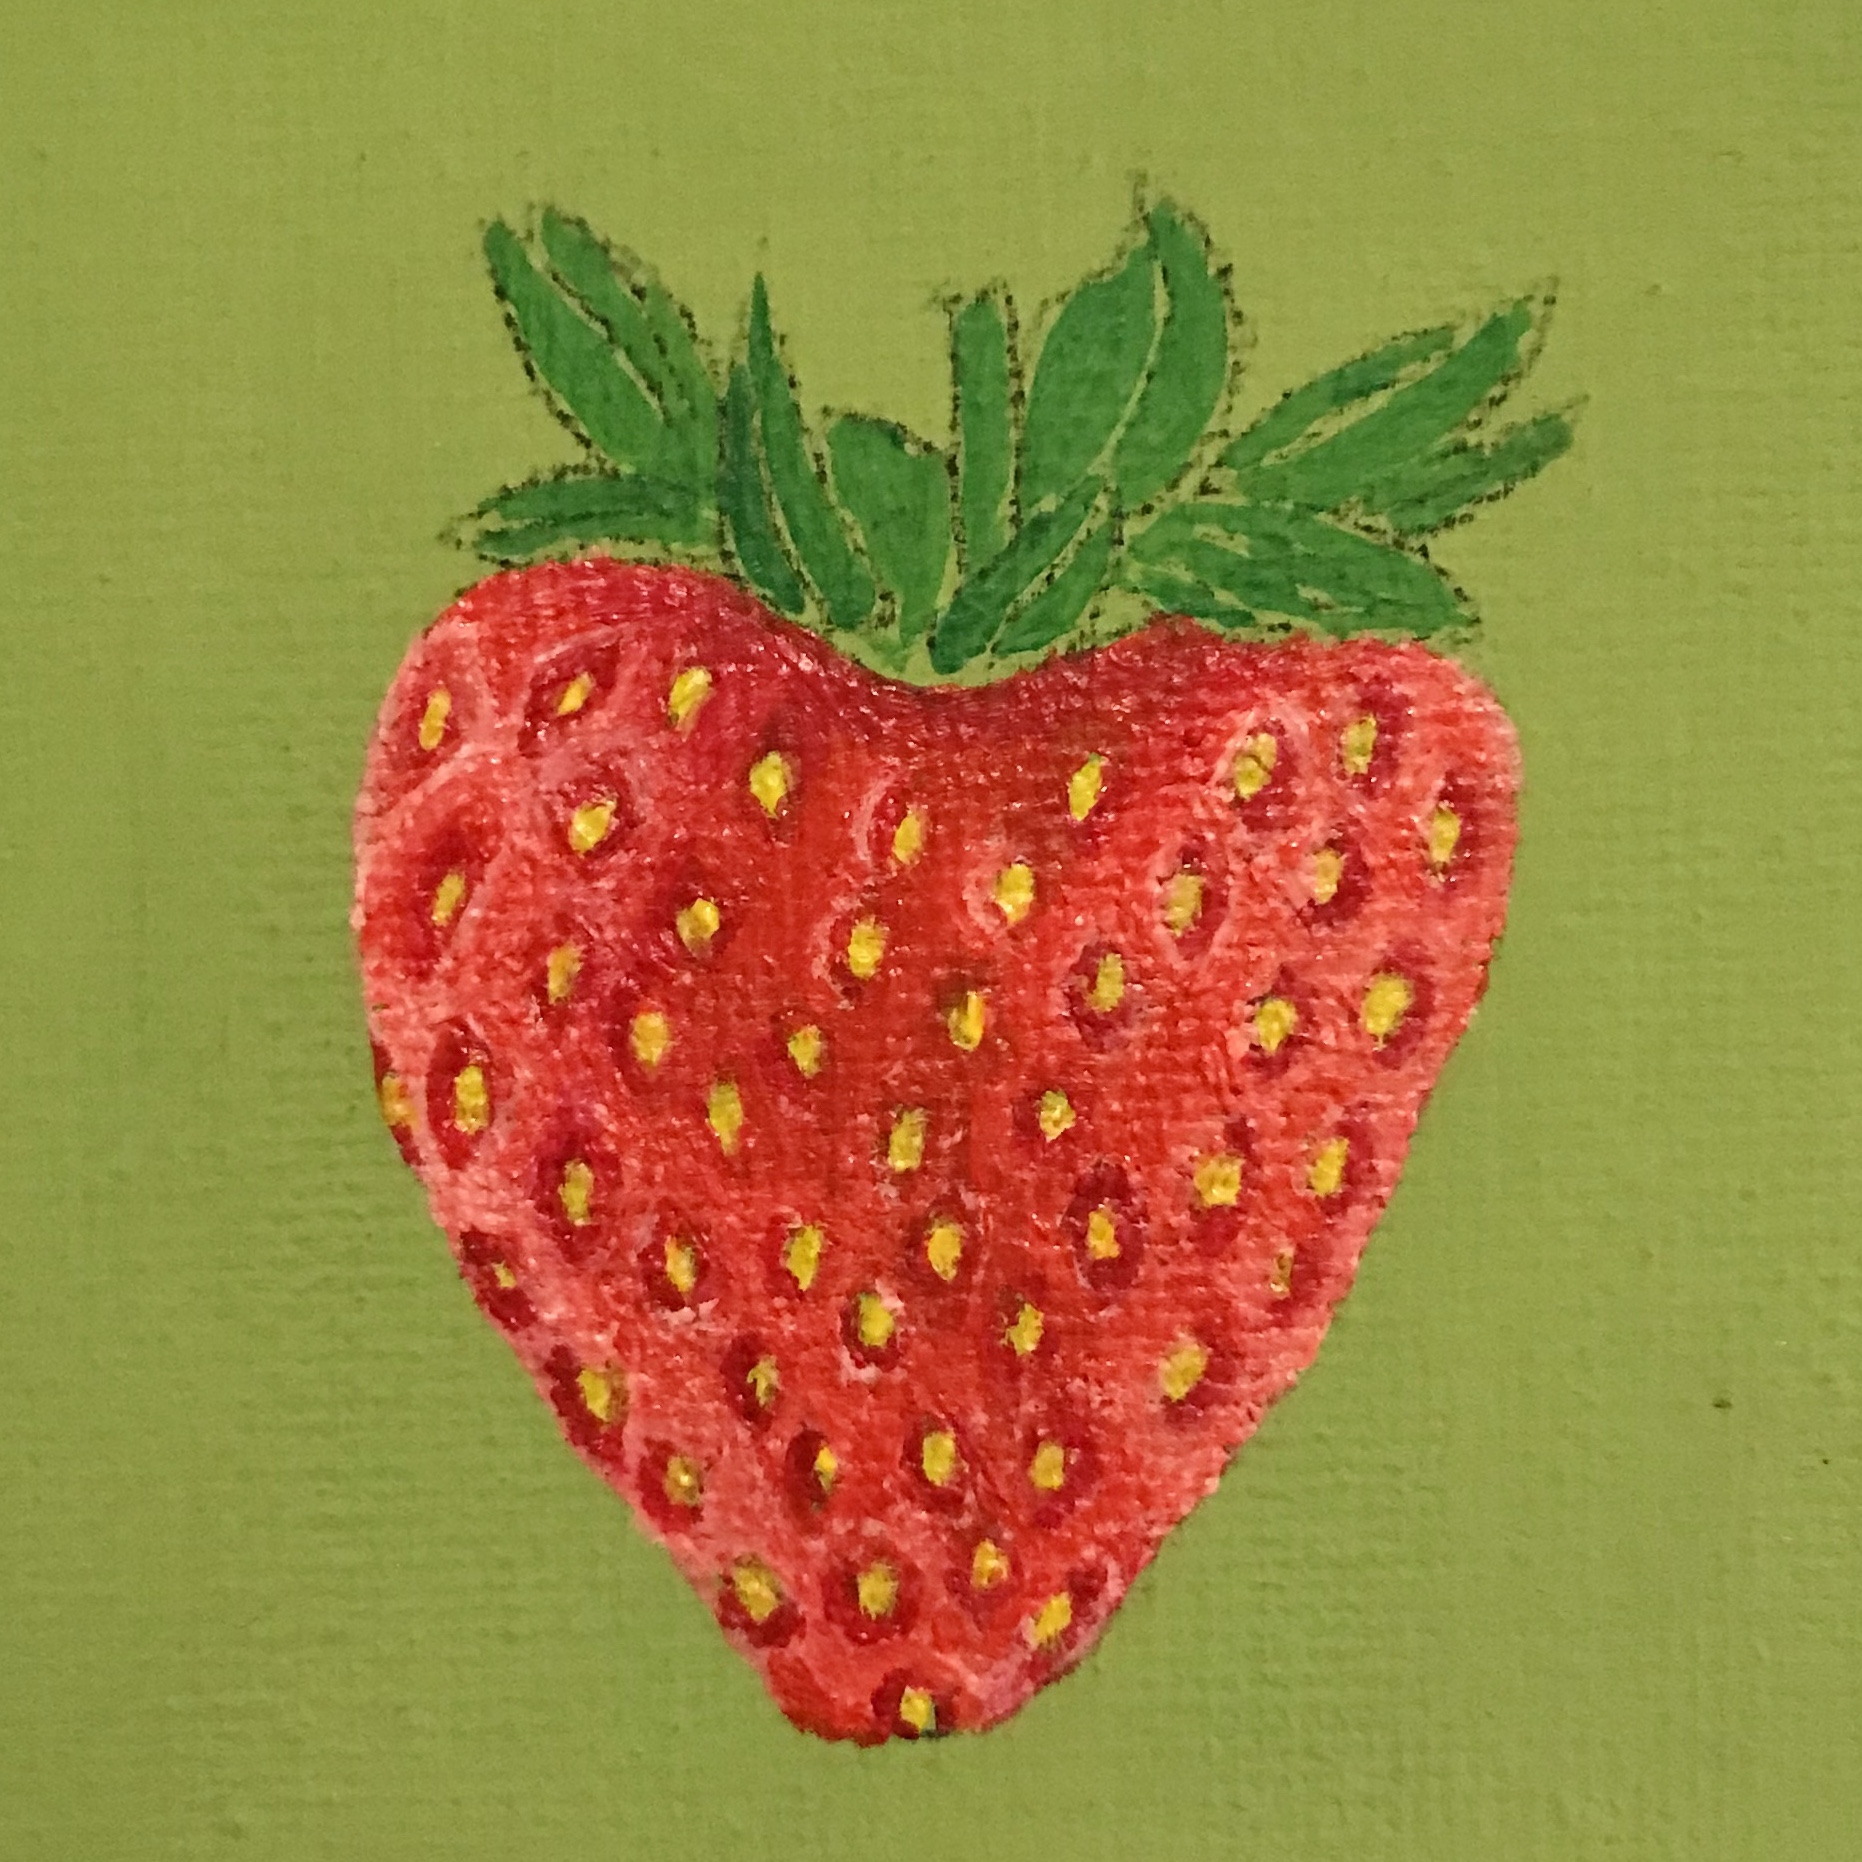
\includegraphics[width=.22\linewidth]{figures/visionscience/fresa_7.jpg}
        8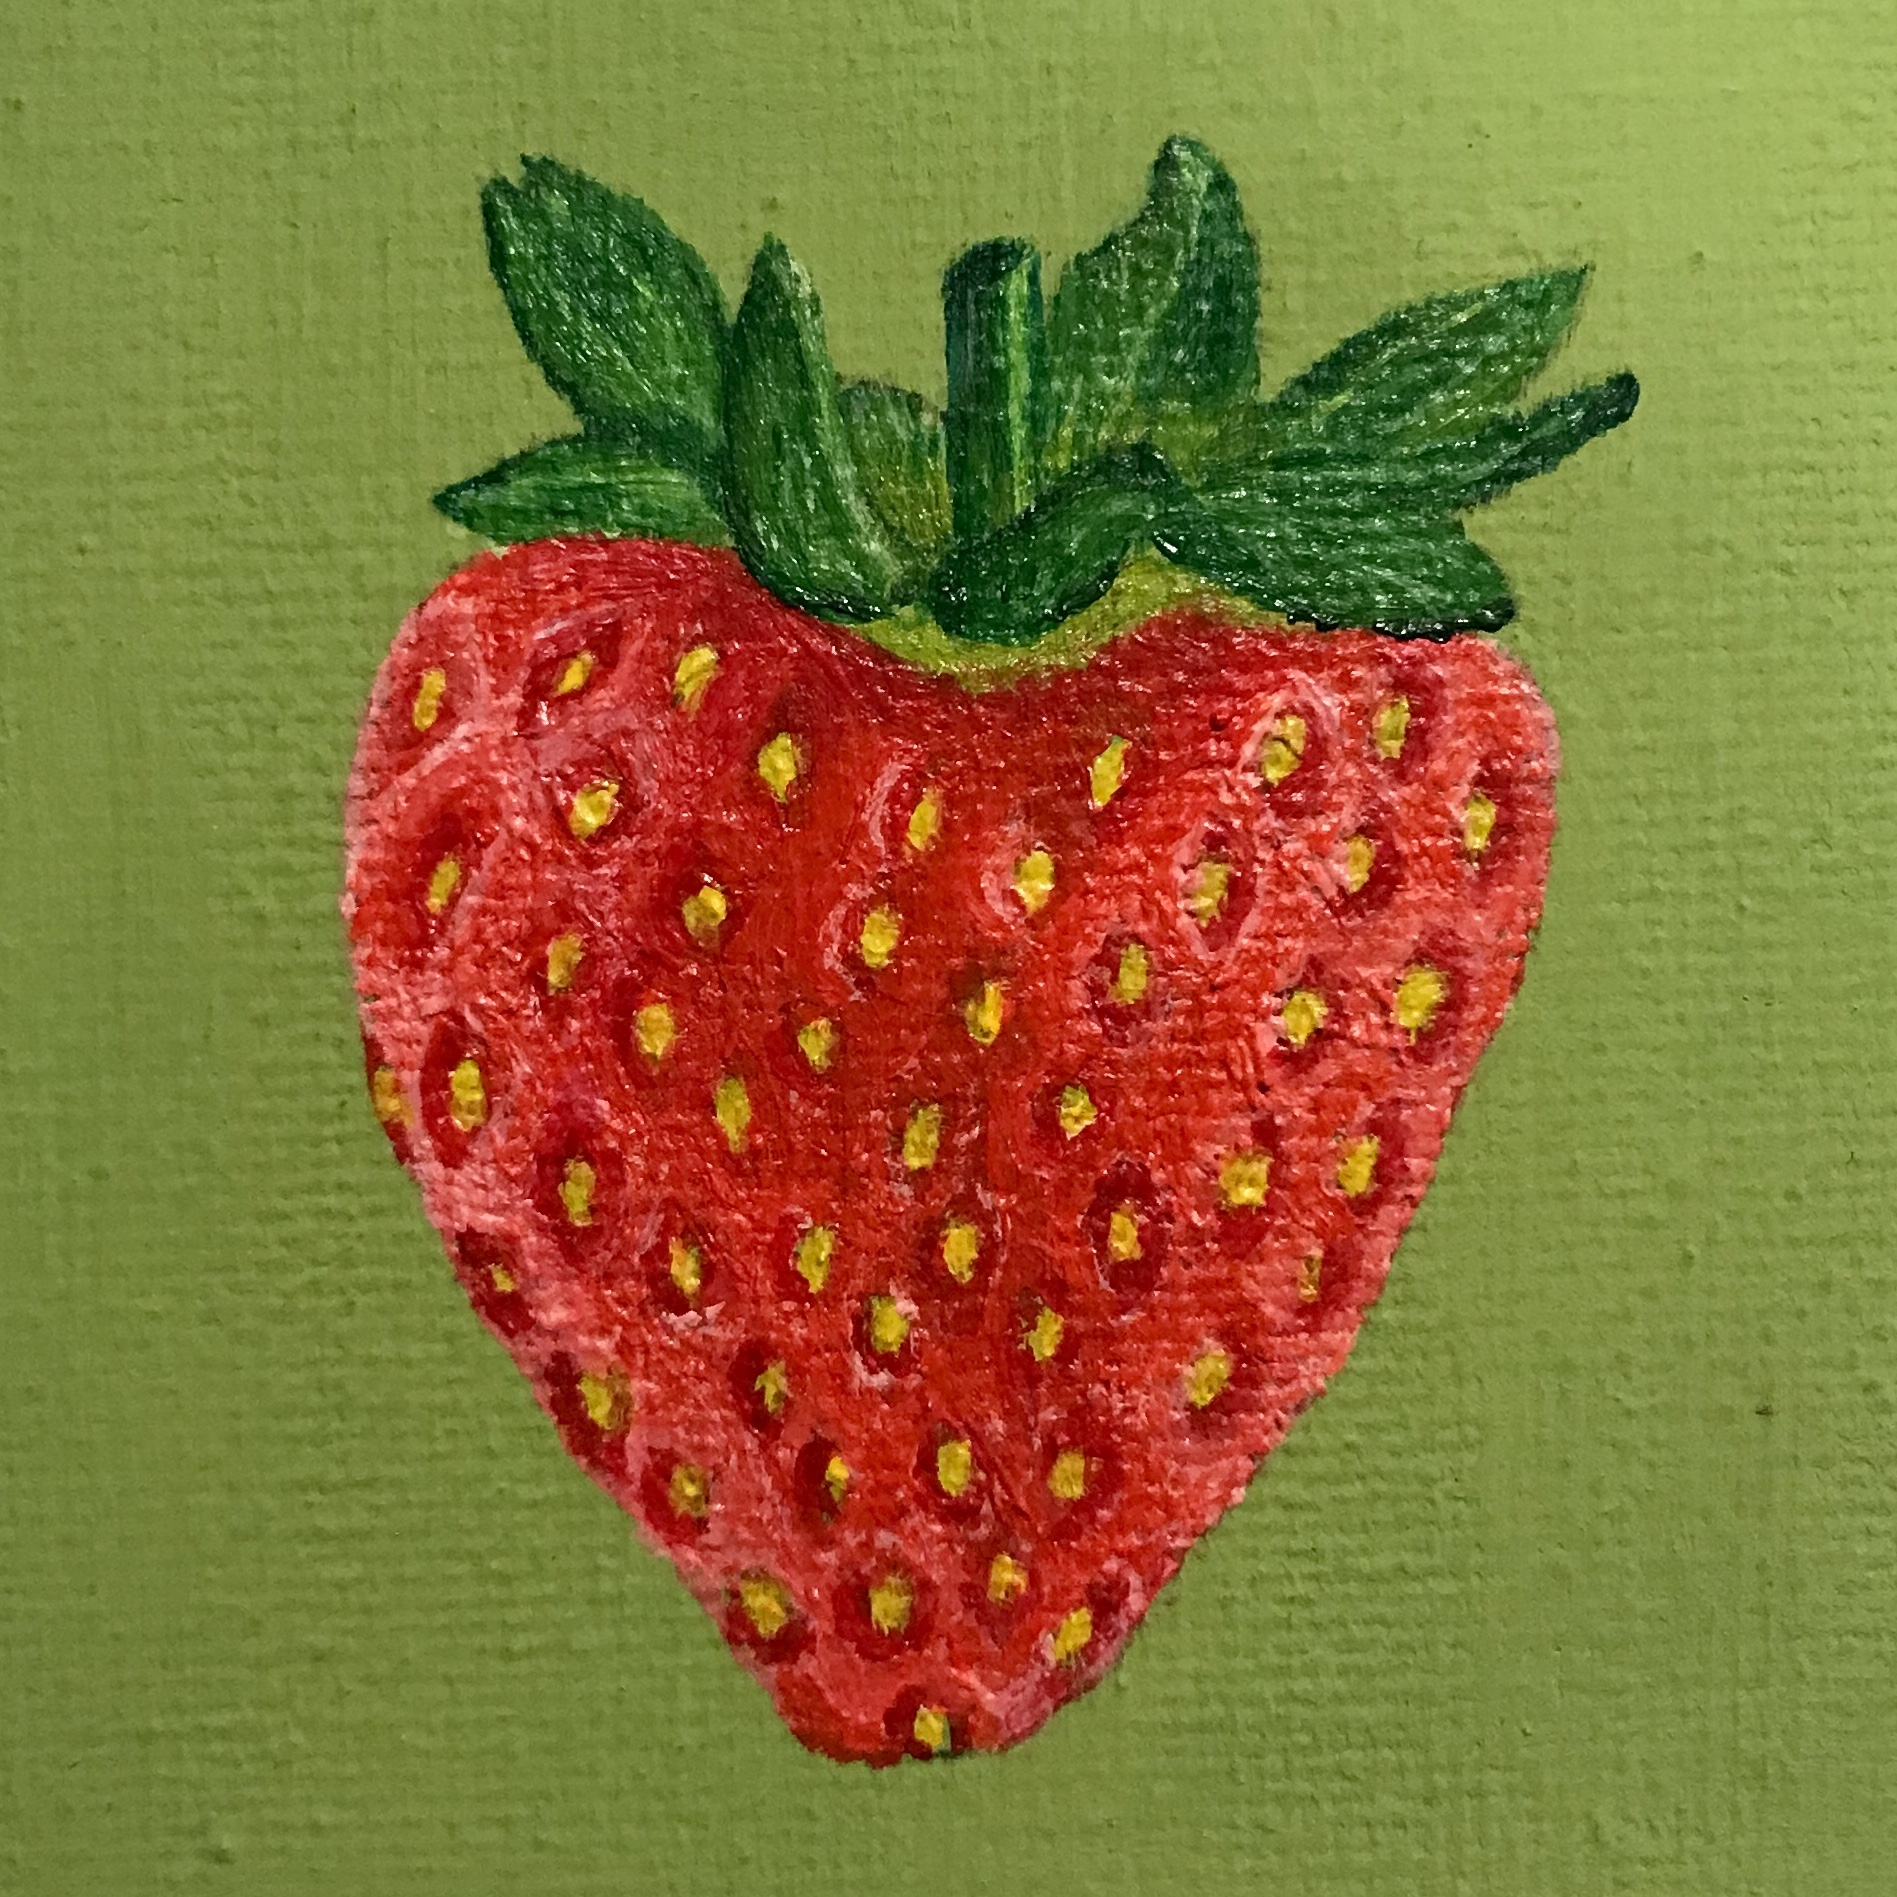
\includegraphics[width=.22\linewidth]{figures/visionscience/fresa_8.jpg} % Photo by Antonio Torralba
    }
    \caption{The following sequence shows different steps in the process of painting a strawberry. {\em Source}: Original images by Agata Lapedriza.}
    \label{fig:agata_painting}
\end{figure}


% \section{Every photo contains thousands of tiny images}
% The image below contains a million pixels, and each is a tiny image.

% \begin{center}
%     patch : image :: image : dataset
% \end{center}

% A common trick in computer vision is to take a method that was developed for processing a \textit{dataset} and instead apply it to the set of patches in an image, or vice versa.


\section{Tree Shadows and Image Formation}

When walking under the shadow of a tree on a bright sunny day when the sun is right above us (\fig{\ref{fig:tree_pinholes}}[left]), we can see how some light rays get through the holes left between leaves, creating spots on the floor (\fig{\ref{fig:tree_pinholes}}[right]).


\begin{figure}[h!]
    \centerline{
        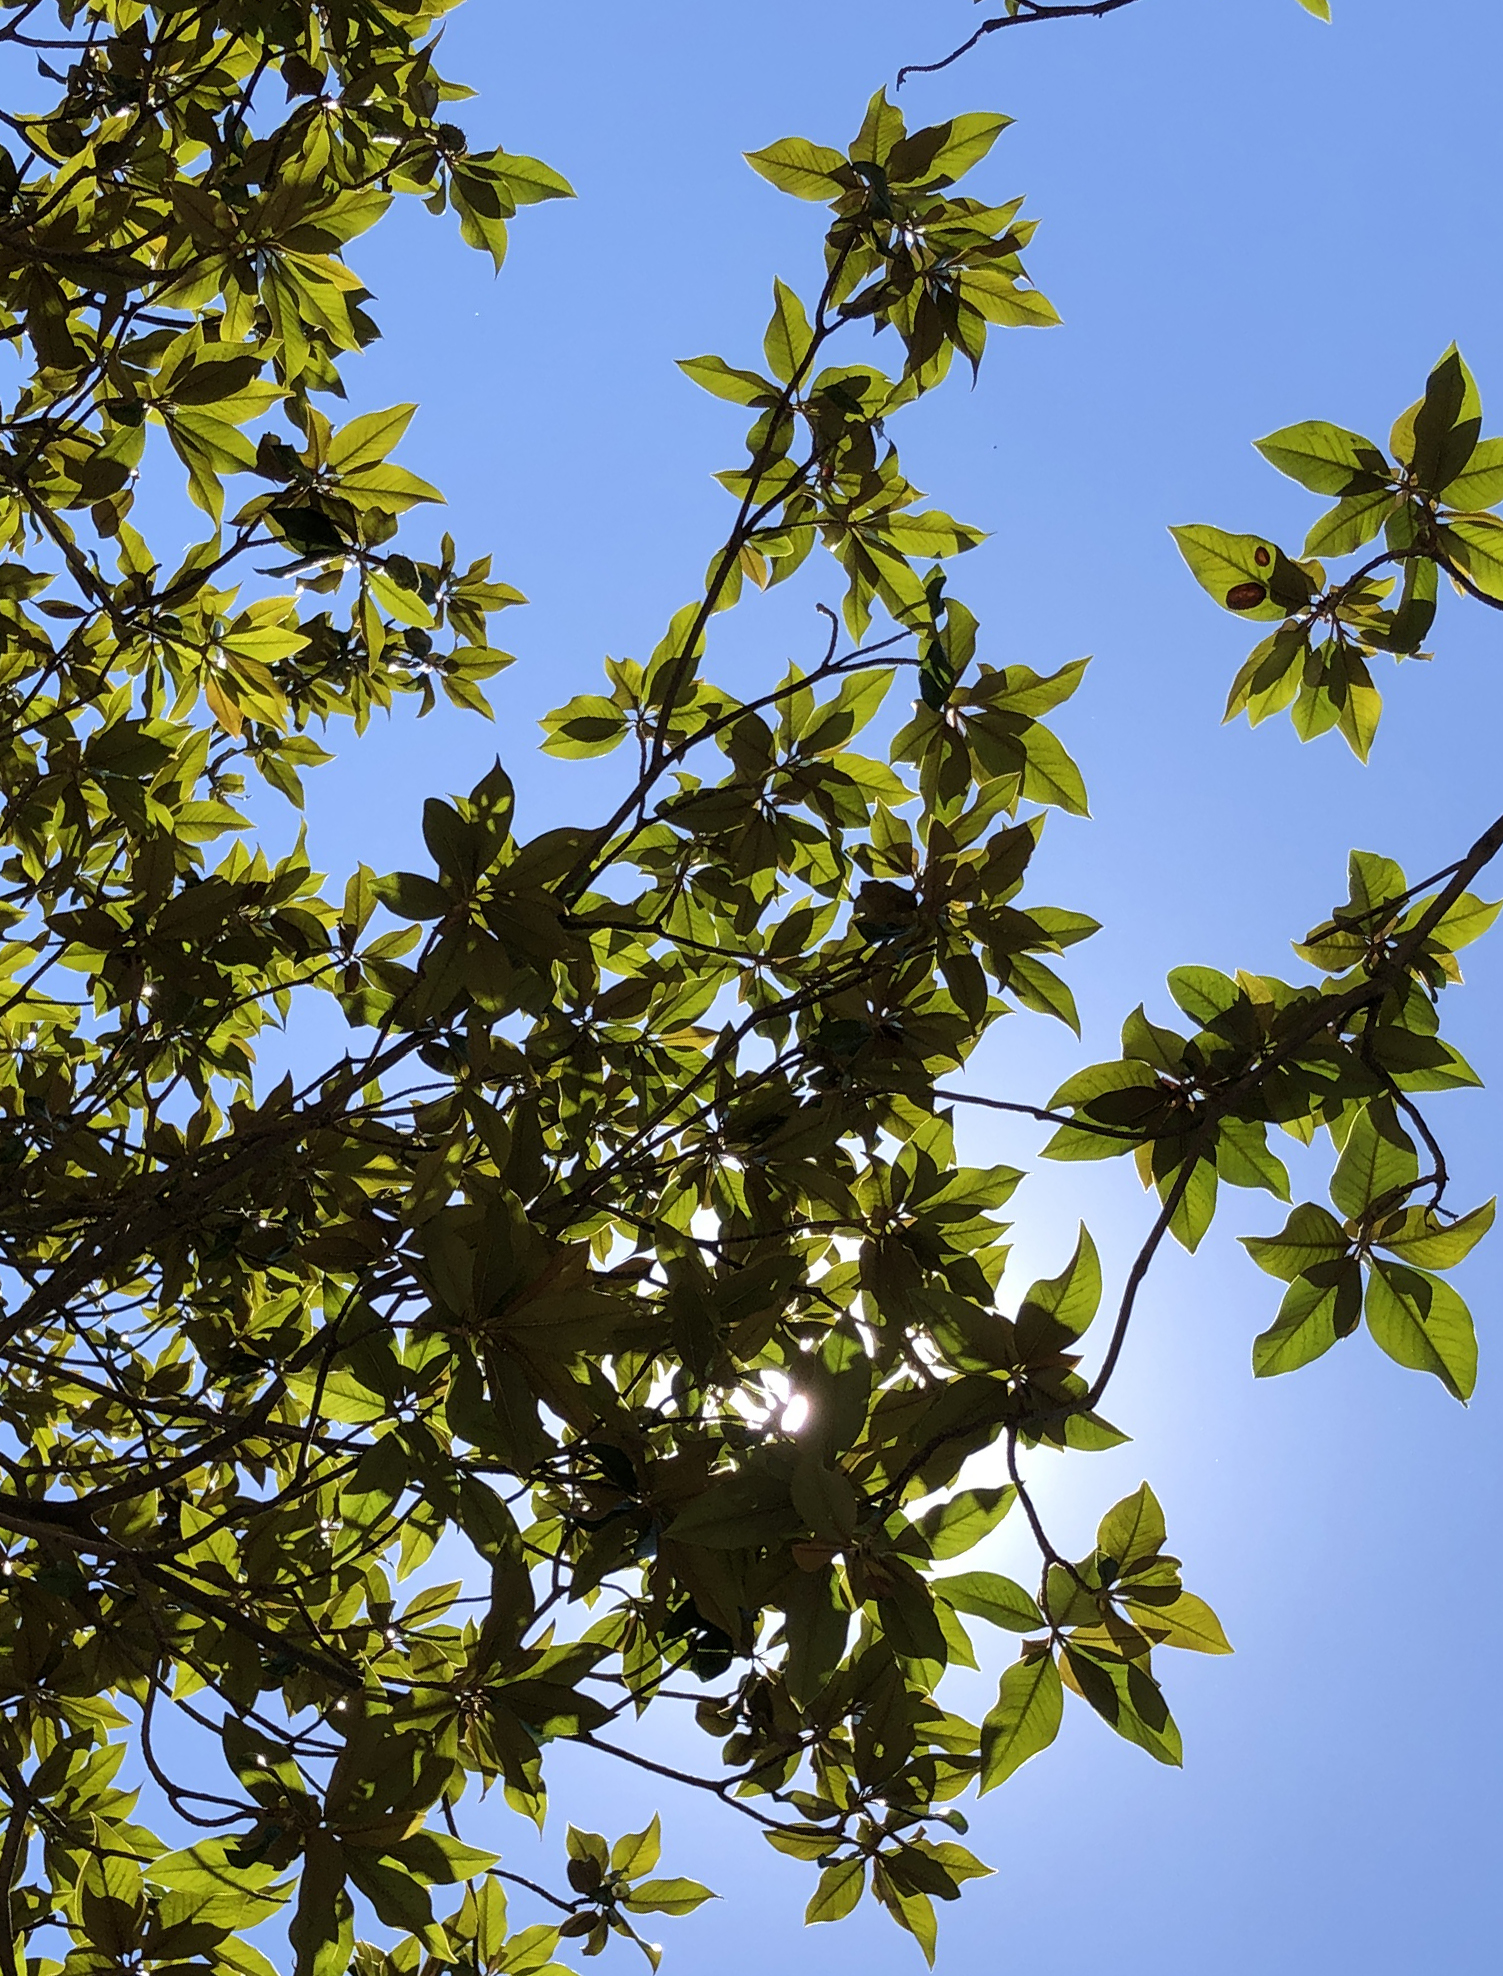
\includegraphics[width=.497\linewidth]{figures/visionscience/IMG_2842_tree_pinholes.jpg} % Photo by Antonio Torralba
        ~~\includegraphics[width=.491\linewidth]{figures/visionscience/IMG_2837_tree_shadow.JPG} % Photo by Antonio Torralba
    }
    \caption{The shadow of this tree on a normal day projects dozens of pictures of the sun on the ground.}
    \label{fig:tree_pinholes}
\end{figure}

But something is a bit odd about the shape of the bright spots projected on the floor. We would expect that the spots of light would have irregular shapes as the openings between leaves will have all kinds of irregular profiles (\fig{\ref{fig:tree_pinholes}}[left]). Instead, as shown in \fig{\ref{fig:tree_pinholes}}(right), the spots appear to be circular and of similar size. This observation already puzzled Aristotle. What could be happening?  As a hint, \fig{\ref{fig:tree_shadow_eclipse}} shows the shadow of leaves during a solar eclipse.


\begin{figure}[h!]
    \centerline{
        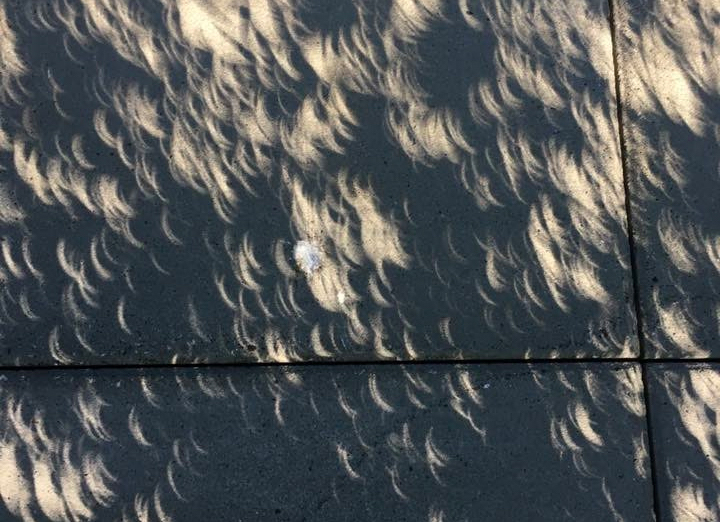
\includegraphics[width=.9\linewidth]{figures/visionscience/tree_shadow_eclipse2.jpg} % Photo by Bill Freeman
    }
    \caption{During an eclipse, the shadow of the tree contains many copies of the crescent sun.}
    \label{fig:tree_shadow_eclipse}
\end{figure}


One of the most common situations that we often encounter is the {\bf pinhole cameras} formed by the spacing between the leaves of a tree.
\index{Camera!Pinhole camera}
The tiny
holes between the leaves of a tree create a multitude of pinholes. The pinholes created by the leaves project different
copies of the sun on the floor. When the openings between leaves are small enough, the shape of the projected spot light is dominated by the shape of the sun.
This is something we see often but rarely think about the origin of the spotlights that we
see on the floor.


%\centerline{
%    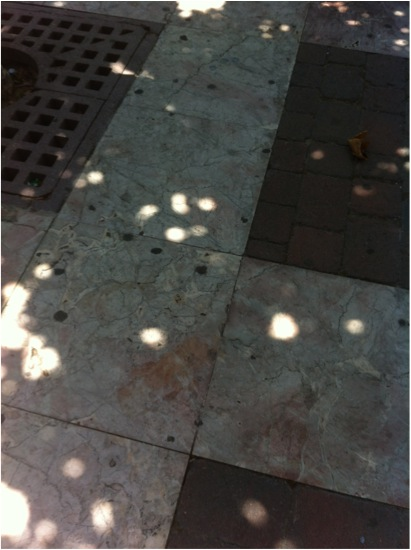
\includegraphics[width=.6\linewidth]{figures/visionscience/trees.jpg}}


In fact, the leaves of a tree create pinholes that produce images in many other situations. We will talk about pinhole cameras in \chap{\ref{chapter:imaging}}.

\section{Horizontal or Vertical}

Looking at the previous picture of the shadow of the tree, another interesting question comes to mind: How do you know you are looking at a picture of the ground? How do you know the orientation of the camera?

Look at the two drawings in \fig{\ref{fig:vertical_or_horizontal}}. The lines in the drawing on the left correspond to tiles in a floor, the line drawing on the right is the same drawing rotated 90 degrees. Which one seems to be an horizontal surface and which one seems vertical? Why? The differences in the line orientations are subtle and yet it produces a very different perception.

\begin{figure}[t]
    \centerline{
        \includegraphics[width=1\linewidth]{figures/visionscience/vertical_or_horizontal.eps}}
    \caption{Line drawings. The one on the left seems to correspond to an horizontal surface while the one on the right looks like a vertical surface.}
    \label{fig:vertical_or_horizontal}
\end{figure}

In the arrangement in the left, there are two {\bf vanishing points} (the points in which parallel lines intersect) and both are above the drawing, compatible with the horizon line. However, on the drawing on the right, one of the vanishing points is below the figure and gives the impression that the camera is looking at a vertical wall (the camera seems to be higher than the visible part of the wall). The horizon line of the plane (the line that connects both vanishing points) is horizontal in the left drawing and vertical on the right one.

%\section{The geometry of vision}




\section{Motion Blur}

When we are in a moving car and we take a picture from the passenger window, often images will appear blurring, specially when taken at night (\fig{\ref{fig:Paris_from_moving_car}}). Blur is due to the fact that the camera sensor is collecting light during a period of time while the car is moving and the picture that results is the average of several translated copies of the same image. However, note that not all of the objects are equally blurry. Things that are far away might still look sharp while things nearby appear very blurry.

\begin{figure}[h!]
    \centerline{
        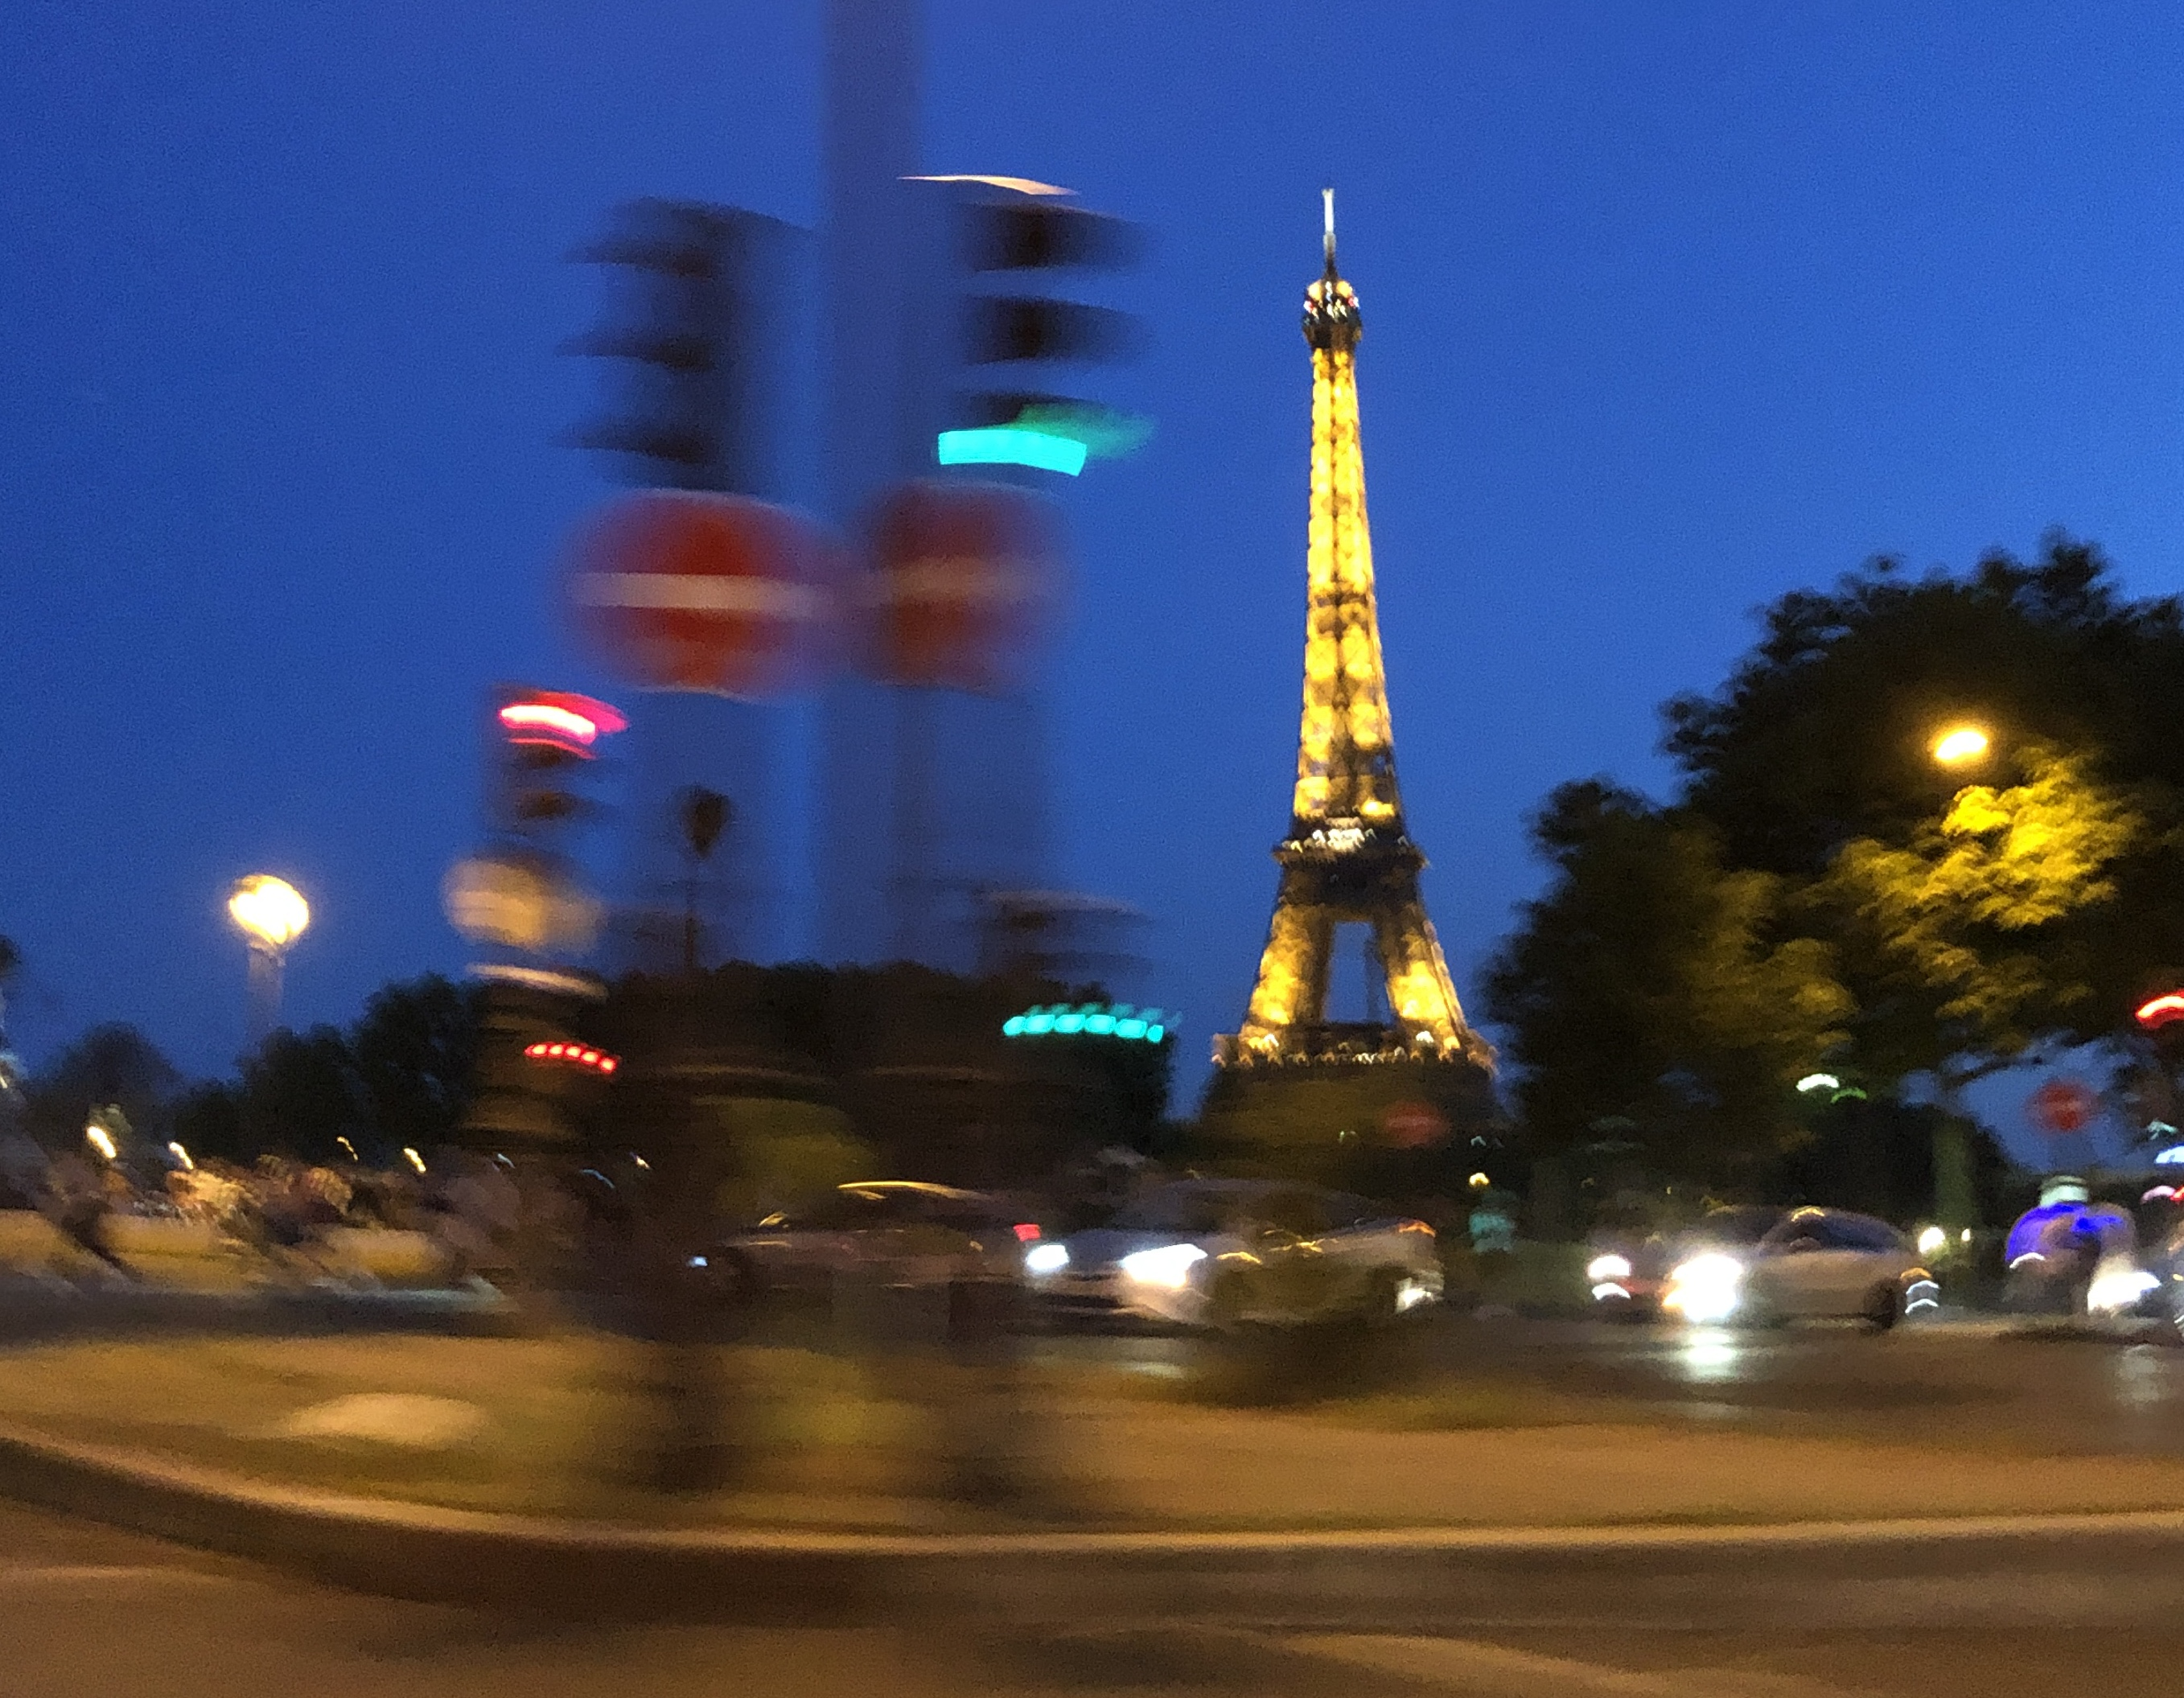
\includegraphics[width=1\linewidth]{figures/visionscience/motion_blur.jpg}} % Photo by Antonio Torralba
    \caption{Picture of Paris taken from a moving car.}
    \label{fig:Paris_from_moving_car}
\end{figure}

The amount of blur is related to the car speed, the exposure time, and the distance between the camera and each object in the scene. We will talk more about how camera motion relates to distance in \chap{\ref{chapter:3D_motion_and_its_2D_projection}}.

\section{Accidents Happen}

\marginnote{Principle of continuity.
    In the following drawing, we see one wave and one line:
    \\[6pt]
    \centerline{
        \includegraphics[width=.6\linewidth]{figures/visionscience/principle_continuity_1.eps}}
    \\[6pt]
    Despite this, other
    groupings are also
    possible.
    \\[6pt]
    \centerline{
        \includegraphics[width=.6\linewidth]{figures/visionscience/principle_continuity_2.eps}}
}
We learned about the generic view principle in \chap{\ref{chapter:simplesystem}}, and this idea comes up a lot in computer vision. But it turns out that in most photographs it's easy to find accidents. This is because photos contain so many things, thousands of tiny images, and there are so many coincidences that could occur. \Fig{\ref{fig:visionscience:migrant_mother}} shows a famous photo and we will look for some coincidences in it. The coincidences are of a specific variety: generically, if you see smooth, continuous line segments you assume that they lie on a single object because it's quite a coincidence for two objects to line up just so their contours perfectly align. The gestalt psychologists called this the {\bf principle of continuity}. The insets  for \fig{\ref{fig:visionscience:migrant_mother}} show several locations in the photo ``Migrant Mother'' by Dorothea Lange where exactly this happens. Can you find more?

\begin{figure}[h!]
    \centerline{
        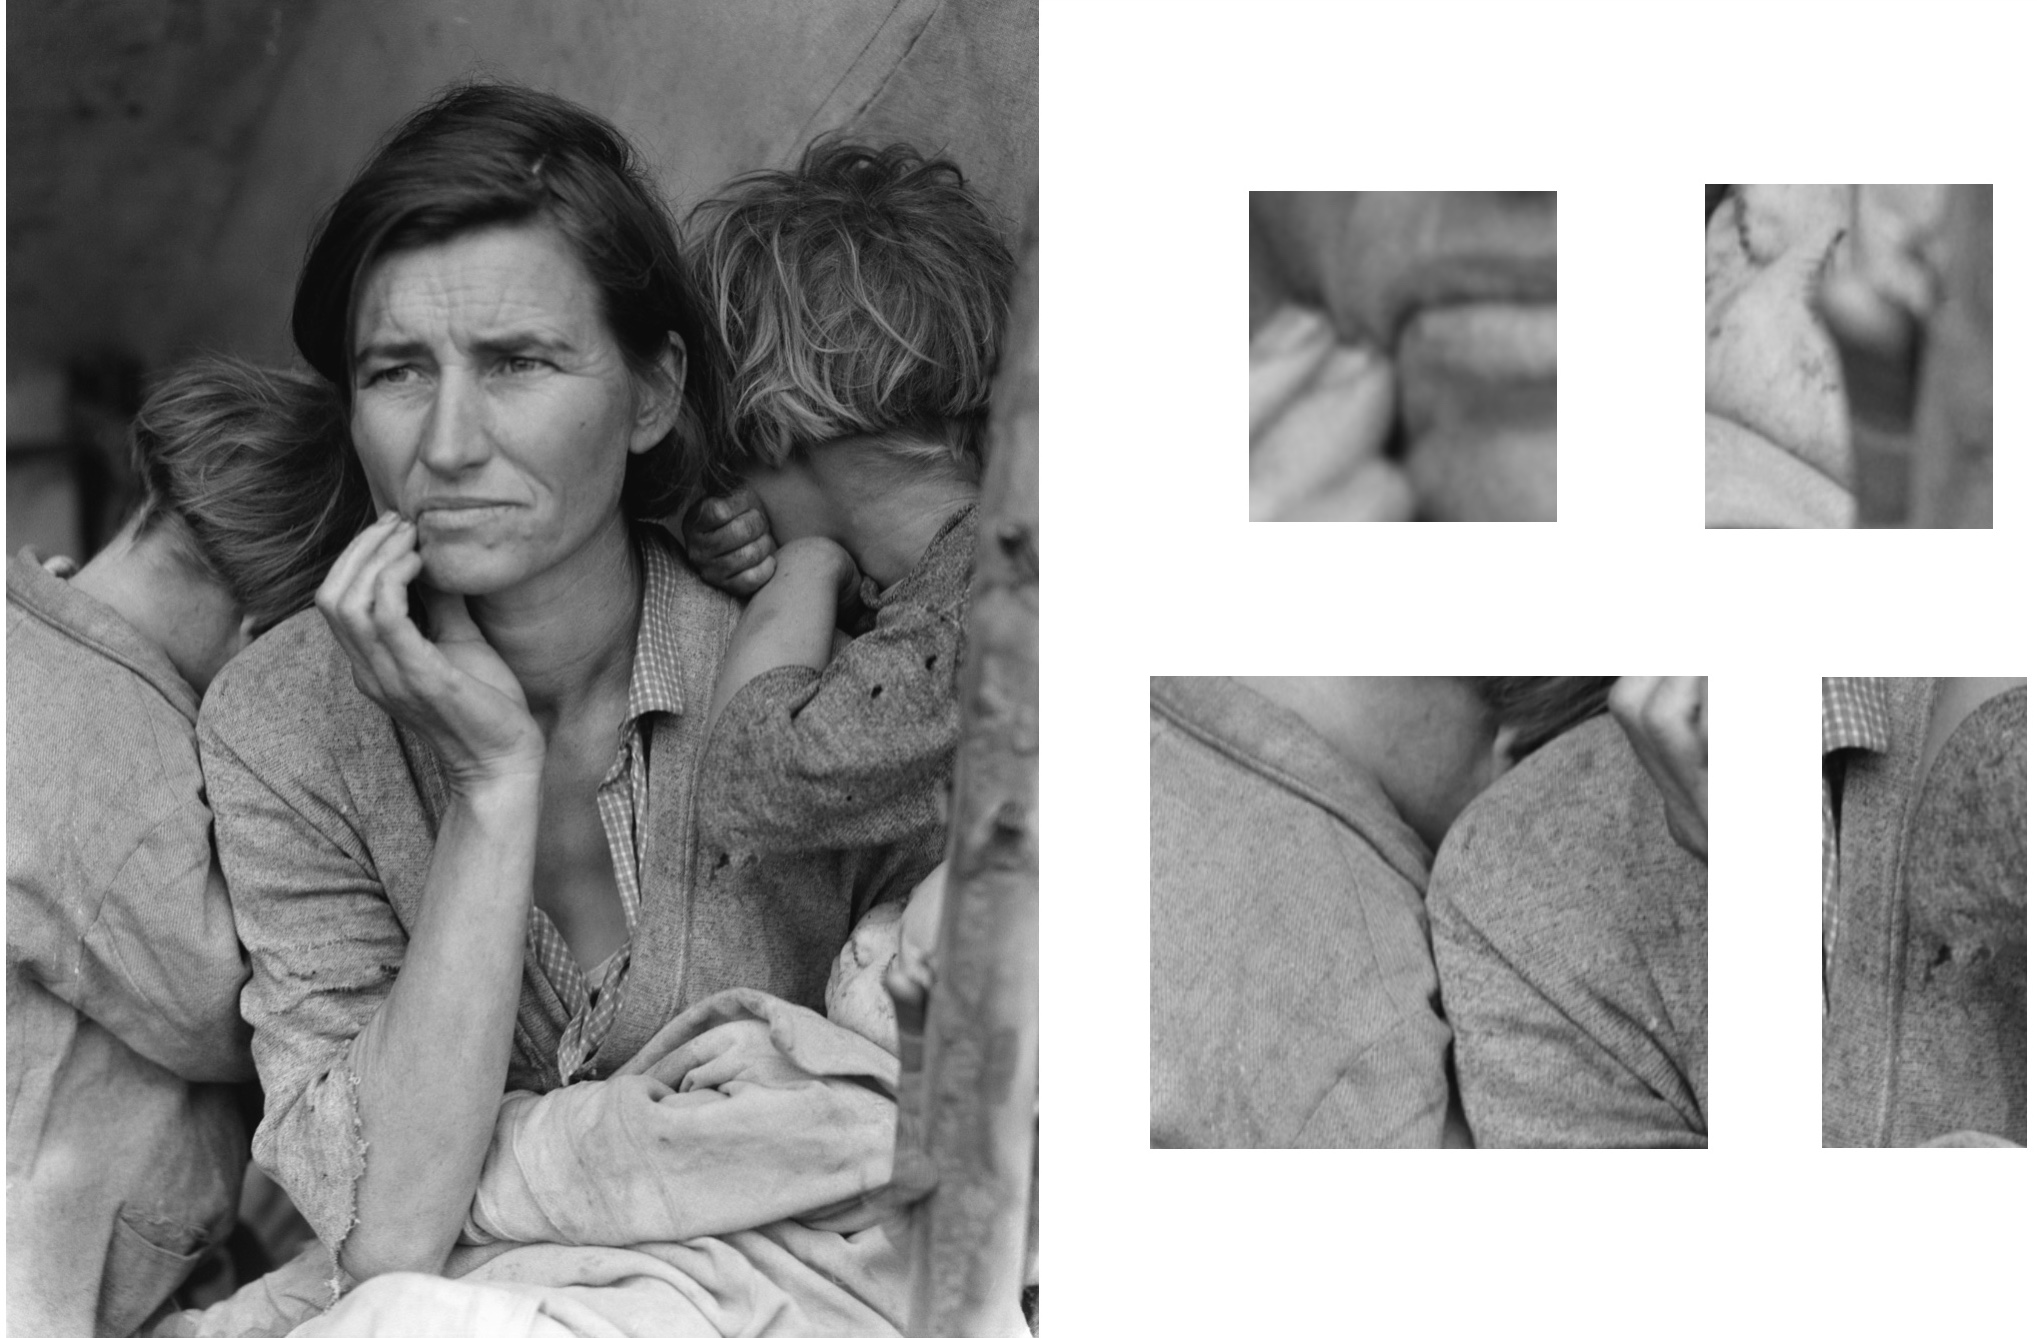
\includegraphics[width=1\linewidth]{figures/visionscience/accidents_migrant_mother.jpg}}
    \caption{Source: Migrant Mother (1936), by Dorothea Lange. On the right are four examples of coincidences that violate the Gestalt principle of continuity. From top-left clockwise: finger boundary aligns with lip contour, cloth aligns with eye, creases align on two different shirts, sleeve boundary is tangent to line on a different shirt.}
    \label{fig:visionscience:migrant_mother}
\end{figure}
% image source: https://en.wikipedia.org/wiki/File:Lange-MigrantMother02.jpg
% license: public domain

You have to be careful about this when developing vision algorithms. If you assume \textit{no} accidents will happen, then you will be in for some trouble. This is one reason why older, rule-based methods failed, because they did not handle exceptions to the rules.




\section{Cues for Support}

When can we tell by looking that one object supports another?  Consider the ball over a surface depicted in \fig{\ref{fig:cues_for_suppport}}.  The drop shadow provides a strong cue that the ball is above the surface in figures \ref{fig:cues_for_suppport}(a) and \ref{fig:cues_for_suppport}(c), while the slack string provides evidence for the ball being on the surface in figures \ref{fig:cues_for_suppport}(b) and \ref{fig:cues_for_suppport}(c).
Only \fig{\ref{fig:cues_for_suppport}}{c} is a doctored photograph.

In which of these figures does the ball appear to be in contact with the ground plane?

\begin{figure}[h!]
    \centerline{
    \sublabel{a}{ \includegraphics[width=0.47\linewidth]{figures/visionscience/ballUp.jpg}
        \sublabel{b}{\includegraphics[width=0.47\linewidth]{figures/visionscience/ballDown.jpg} }
    }
    \centerline{
        \sublabel{c}{\includegraphics[width=0.47\linewidth]{figures/visionscience/ballPuzzle.jpg}}
    }
    \caption{Cues for support. The relative location between an object, and its shadow on the ground is a powerful cue for contact.}
    \label{fig:cues_for_suppport}
\end{figure}
% image source: photos by Bill


\section{Looking at Raindrops}

When it rains you get to see a rare sight. Every raindrop refracts a panorama of the scene around it (\fig{\ref{fig:droplets}}). What you are seeing is not just one photo but hundreds of images of the scene, one in each raindrop, all from slightly different angles. It turns out specially designed cameras have been made that do the same thing, and they are called {\bf light field cameras}.
\index{Camera!Light field cameras}
These cameras use an array of tiny lenses rather than raindrops, but the result is similar: they capture what the scene looks like from hundreds of different viewing angles, and from that density of information they can achieve many interesting tricks, such as triangulating the depth of objects in the scene and synthetically refocusing the image after it has been taken.

\begin{figure}[t]
    \centerline{
        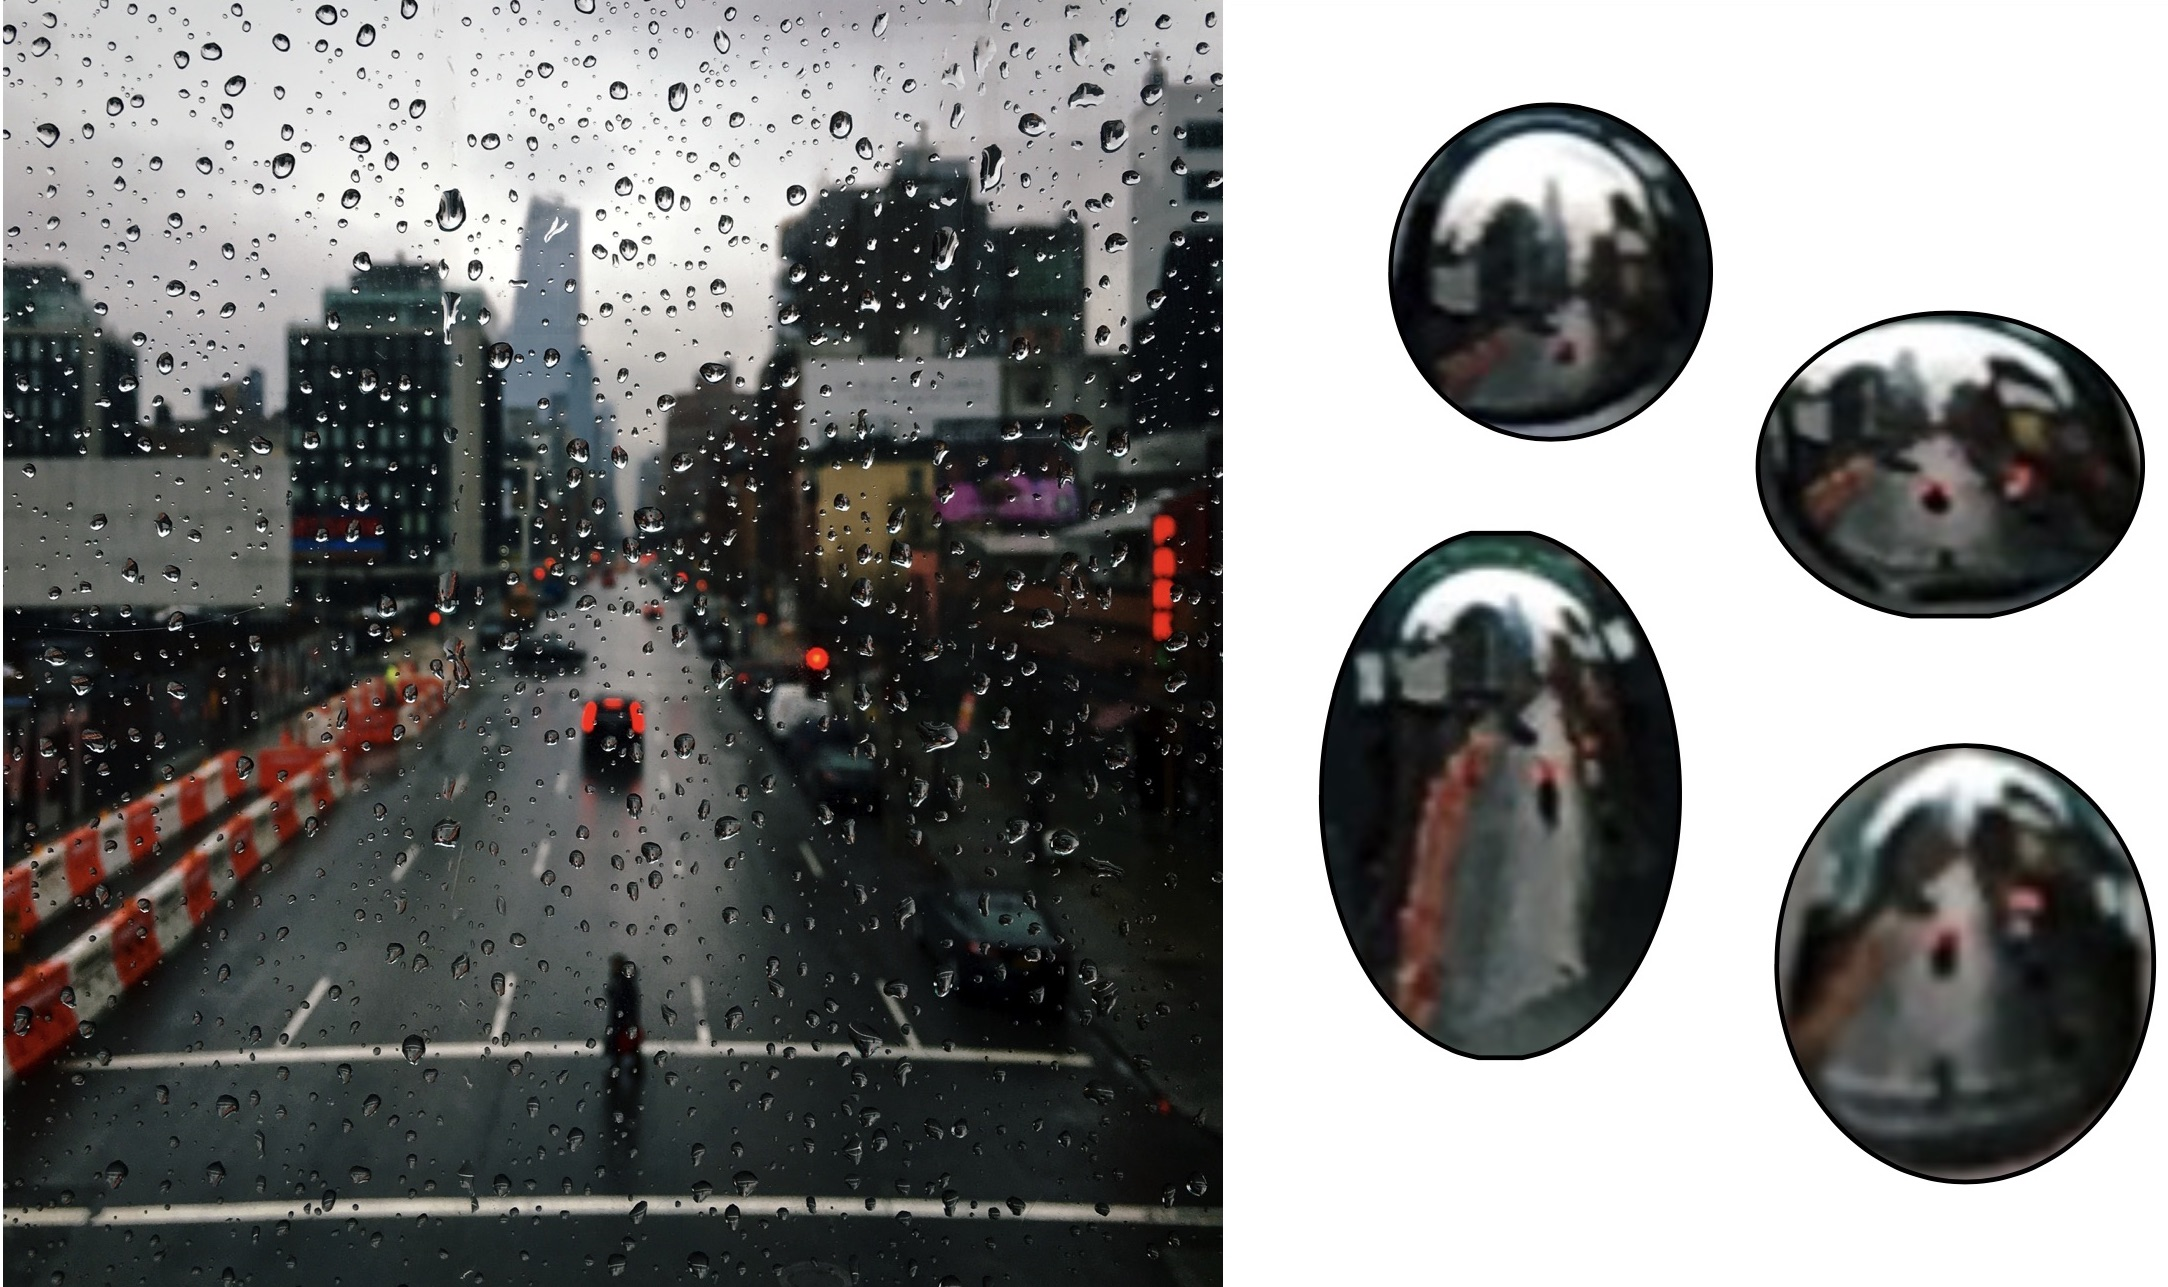
\includegraphics[width=1.0\linewidth]{figures/visionscience/droplets.jpg}}
    \caption{A naturally occurring light field camera. This picture of raindrops on a window contains hundreds of tiny images of the scene, one in each raindrop. The images to the right are individual zoomed in raindrops from the photo on the left.}
    \label{fig:droplets}
\end{figure}
% Photo by Phillip Isola


\section{Plato's Cave}

% \begin{figure}[h]
% \centerline{
%      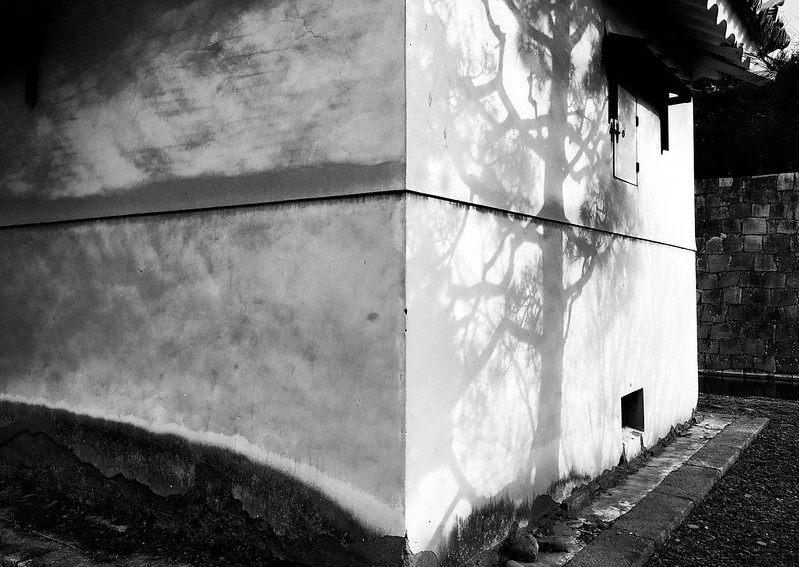
\includegraphics[width=0.8\linewidth]{figures/visionscience/fading_shadows.jpg}}
%      \caption{Vision is analogous to Plato's Allegory of the Cave.  An image is a crude projection of the underlying physical state.}
%  \end{figure}
% % Photo by Phillip Isola

In the \textit{Allegory of the Cave}, Plato imagined a group of prisoners
chained up in a cave whose only experience of the outside world is through shadows cast on the cave's wall.
When we look at images, we think we are directly seeing reality, but actually the situation is much more like Plato's cave. An image is a crude projection of the underlying physical state. It collapses all the 3D geometry into a flat 2D grid of pixels. From any given viewing angle, most of the scene is occluded. Materials are only depicted in terms of how photons bounce off their surfaces; what's below the surface may be completely omitted. When you look at a picture, think about all the things you cannot see. There's more you don't see than you do. One job of a vision system is to infer everything you can't see given everything you can.

\marginnote{The allegory of the cave has several layers of indirection: the shadows are cast by puppets that are controlled by puppeteers who act out interpretations of the broader reality outside.}

\section{How Do You Know Something Is Wet?}

Our visual system allows us to recognize not just objects, but also material. We can tell if something will feel hot or cold, soft or hard, smooth or rugged. We can also recognize if something is wet or not without touching it, as shown in \fig{\ref{fig:wet_sand}}.



\begin{figure}[t]
    \centerline{
        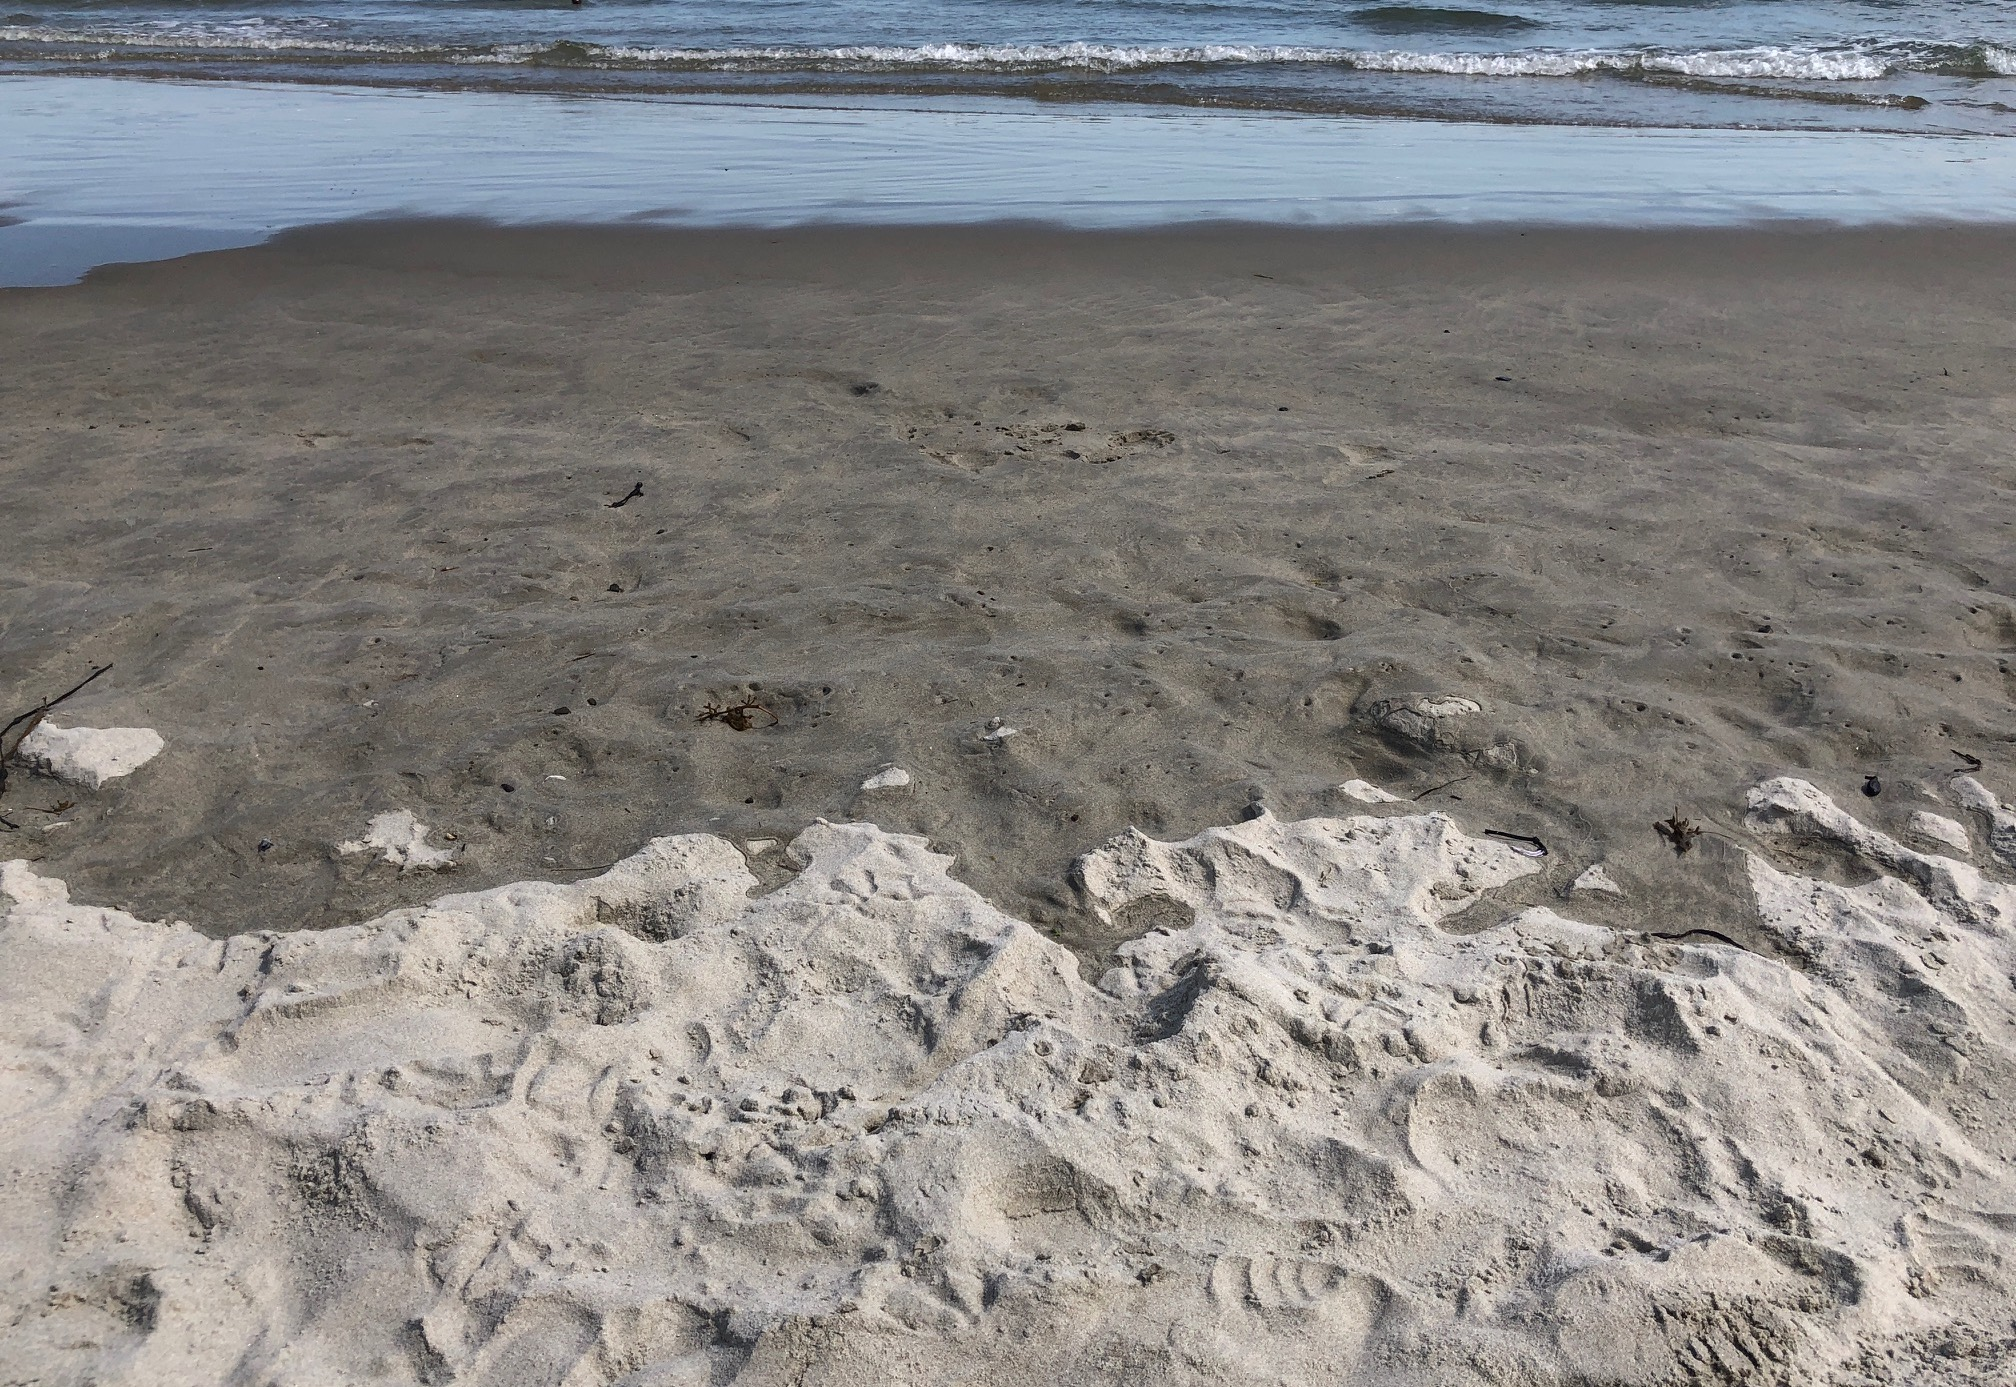
\includegraphics[width=.8\linewidth]{figures/visionscience/wet_sand_2.jpeg}}
    \caption{Why does wet sand look dark? The answer to this question is interesting, but not as much as the question itself.}
    \label{fig:wet_sand}
\end{figure}
% Photo by Antonio Torralba


Why does sand look darker when it's wet? Does everything wet look darker than when it is dry? How can we tell which parts of the sand are dark because they are wet and which ones are dark because they are under a shadow?


\section{Concluding Remarks}

This chapter was about learning to ask questions about what we see, why things look the way they do, and how do we recognize them. There are so many things that we see every day that we recognize by the way they look, and yet we seldom ask ourselves why they look that way. Why does the sky appear blue? Why does the moon always look the same? Why do hot things become redder?
There are many other sources you can consult that explore why things look the way they do in the world. A beautiful book on this topic is \booktitle{Light and Color in the Outdoors} by Marcel Minnaert \cite{Minnaert1993}, first published in 1937.

After reading this chapter, you will not know how to implement anything new, nor will you have learned new math or new algorithms. The goal of this chapter was to show you some of the questions you should ask about the visual world that you experience every day. The exercise to do now is to go around with your camera and take pictures of interesting visual phenomena.

\marginnote{Your brain is like a detective looking at all the clues that reveal what the world is made of.}

%% %% jan. 4, 2011  items to fix:
%% notation for math and reference to images.
%% how include eps figures.
%% make all the little figures (search for eps) in a common, nice matlab way for the
%% example filtering operations.

%% Material:
% Michael Black tutorial 2014: https://www.youtube.com/watch?v=tIwpDuqJqcE

\chapter{Optical Flow Estimation}
\label{chap:optical_flow_estimation}


\section{Introduction}

Now that we have seen how a moving three-dimensional (3D) scene (or camera) produces a two-dimensional (2D) motion field on the image, let's see how can we measure the resulting 2D motion field using the recorded images by the camera. We want to measure the 2D displacement of every pixel in a sequence.


Unfortunately, we do not have a direct observation of the 2D motion field either, and not all the displacements in image intensities correspond to 3D motion. In some cases, we can have scene motion without producing changes in the image, such as when the camera moves in front of a completely white wall; in other cases, we will see motion in the image even when there is not motion in the scene such as when the illumination source moves.

In the previous chapter we discussed a matching-based algorithm for motion estimation but it is slow and assumes that the motion is only on discrete pixel locations. In this chapter we will discuss gradient-based approaches that allow for estimating continuous displacement values. These methods introduce many of the concepts later used by learning-based approaches that employ deep learning.


\section{2D Motion Field and Optical Flow}

Before we discuss how to estimate motion, let's introduce a new concept: optical flow. \marginnote{James J. Gibson, presented in chapter \ref{chap:challenge_of_vision}, introduced the concept of optical flow in 1947 \cite{gibson1947motion}.}

{\bf Optical flow}\index{Optical flow} is an approximation to the 2D motion field computed by measuring displacement of image brightness (\fig{\ref{fig:visualization_optical_flow}}). The ideal optical flow is defined as follows: given two images $\boldimg_1$ and $\boldimg_2$ $\in \mathbb{R}^{N \times M \times 3}$, the optical flow $\left[ \mathbf{u}, \mathbf{v} \right] \in \mathbb{R}^{N \times M \times 2}$ indicates the relative position of each pixel in $\boldimg_1$ and the corresponding pixel in $\boldimg_2$. Note that optical flow will change if we reverse time. This definition assumes that there is a one-to-one mapping between two frames. This will not be true if an object appears in one frame, or when it disappears behind occlusions. The definition also assumes that one motion explains all pixel brightness changes. That assumption can be violated for many reasons, including, for example, if transparent objects move in different directions, or if an illumination source moves.


\Fig{\ref{fig:visualization_optical_flow}} shows two frames and the optical flow between them. This visualization using a color code was introduced in \cite{Baker2007}. In this chapter we will use arrows instead as it provides a more direct visualization and it is sufficient for the examples we will work with.

\begin{figure}[t]
    \centerline{
        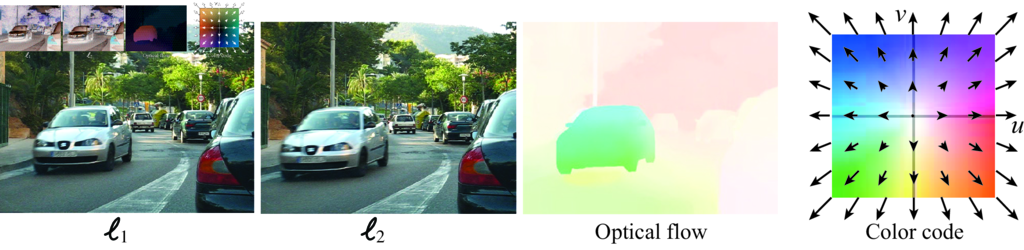
\includegraphics[width=1\linewidth]{figures/optical_flow/visualization_optical_flow.eps}}
    \caption{Two frames of a sequence, ground-truth optical flow (color coded), and the color code to read the vector at each pixel.}
    \label{fig:visualization_optical_flow}
\end{figure}

%http://www.cs.toronto.edu/~fleet/research/Papers/flowChapter05.pdf

% Visualization optical flow from:
%S. Baker, D. Scharstein, J. Lewis, S. Roth, M. J. Black, and R. Szeliski.
%A database and evaluation methodology for optical flow.
%In Proc. IEEE International Conference on Computer Vision (ICCV), 2007.

%{\bf Scene flow} is the estimation of the 3D motion field. Ultimately, we are interested in using motion information to recover the camera motion, the 3D structure of the scene and the 3D motion of objects. 

%In chapter \ref{chapter:temporal_filters} we discussed energy-based approaches which estimate motion by modeling how the energy of spatio-temporal filters varies as a function of input motion. 

\subsection{When Optical Flow and Motion Flow Are Not the Same}

There are a number of scenarios where motion in the image brightness does not correspond to the motion of the 3D points in the scene. Here there are some examples where it is unclear how motion should be defined:

\begin{itemize}
    \item Rotating Lambertian sphere with a static illumination will produce no changes in the image. If the sphere is static, and the light source moves, we will see motion in spite of the sphere being static.

    \item Moving in front of a textureless wall produces no change on the image.

    \item Waves in water: waves appear to move along the surface but the actual motion of the water is up and down (well, it is even more complicated than that).

    \item A rotating mirror will produce the appearance of a faster motion. And this will happen in general with any surface that has some specular component.

    \item A camera moving in front of a specular planar surface will not produce a motion field corresponding to a homography.
\end{itemize}

Motion estimation should not just measure pixel motion, it should also try to assign to each source of variation in the image the physical cause for that change. The models we will study in this chapter will not attempt to do this.

\subsection{The Aperture Problem}

One classical example of the limitations of motion estimation from images is the {\bf aperture problem}. \index{Aperture problem}
The aperture problem happens when observing the motion of a one-dimensional (1D) structure larger than the image frame, as shown in \fig{\ref{fig:apperture_problem}}. If none of the termination points are in view within the observation window (i.e., the aperture), it is impossible to measure the actual image motion. Only the component orthogonal to the moving structure can be measured.


\begin{figure}[t]
    \centerline{
        \includegraphics[width=.9\linewidth]{figures/optical_flow/apperture_problem.eps}}
    \caption{Aperture problem when observing the motion of a one-dimensional (1D) structure larger than the image frame. The actual motion of the bar is upward, but the perception, when vision is limited to what is visible within the observation window, appears as if the motion of the bar is in the direction perpendicular to the bar.}
    \label{fig:apperture_problem}
\end{figure}



\marginnote{The {\bf Barber-pole illusion} is an illustration of the aperture problem. The barber pole induces the illusion of downward motion while rotating.
    \\[6pt] \index{Barber-pole illusion}
    \centerline{
        \includegraphics[width=.2\linewidth]{figures/optical_flow/barber_pole.eps}
    }
    %\begin{figure}
    %\centerline{
    %\includegraphics[width=1\linewidth]{figures/optical_flow/barber_pole.eps}
    %}
    %\end{figure}
}[-1in]



\subsection{Representation of Optical Flow}

We can model motion over time as a sequence of {\bf dense optical flow} \index{Dense optical flow} images:
\begin{equation}
    \left[ u(x,y,t), v(x,y,t) \right]
\end{equation}
The quantities $u(x,y,t)$ and $v(x,y,t)$ indicate that a pixel at image coordinates $(x,y)$ at time $t$ moves with velocity $(u,v)$. The problem with this formulation is that we do not have an explicit representation of the trajectory followed by points in the scene over time. As time $t$ changes, the location $(x,y)$ might correspond to different scene elements.


An alternative representation is to model motion as a {\bf sparse set of moving points} (tracks):
\begin{equation}
    \left\{ \mathbf{P}^{(i)}_t \right\}_{i=1}^N
\end{equation}
This has the challenge that we have to establish the correspondence of the same scene point over time (tracking). The appearance of a 3D scene point will change over time due to perspective projection and other variations such as illumination changes over time. It might be difficult to do this on a dense array. Therefore, most representations of motion as sets of moving points use a sparse set of points.



Both of those motion representations have limitations, and depending on the applications, one representation may be preferred over the other. Choosing the right representation might be challenging in certain situations. For instance, what representation would be the most appropriate to describe the flow of smoke or water over time? (We do not know the answer to this question, and the answer might depend on what do we want to do with it.)

In the rest of this chapter we will use the dense optical flow representation.


\section{Model-Based Approaches}

Let's now describe a set of approaches for motion estimation that are not based on learning. Motion estimation equations will be derived from first principles and will rely on some simple assumptions.

In section \ref{sec:matching_based_motion} we discussed matching-based optical flow estimation. We will discuss now gradient-based methods. These approaches rely on the brightness constancy assumption and use the reconstruction error as the loss to optimize. %The two approaches briefly discussed here differ on the space of functions used to describe the optical flow.




%The {\bf constant brightness assumption} says that, as a scene element moves in the world, the brightness captured by the camera does not change over time. In math, this assumption translates into the following relationship: given two frames $f_1$ and $f_2$ of a video we can write:
%\begin{eqnarray}
%f_2 (x,y) &=& f_1 (x-u,y-v) + n(x,y) \\
%n(x,y) & \sim & \mathcal{N}(0,\,\sigma^{2})
%f (x,y,t) = f (x-u(t),y-v(t), 0) + n
%\end{eqnarray}

%where $u$ and $v$ are the pixel displacement over time and are also a function of pixel location, $u(x,y)$ and $v(x,y)$. The only pixel brightness variations over time will be due to zero mean iid Gaussian noise, $n(x,y)$, introduced by the camera. 



%Let's start with the formulation of the brightness constancy assumption. One way of expressing the constancy brightness assumption is to say that the sequence $f(x,y,t)$ does not change its appearance when it translates. Therefore, from one frame to the next ($t -> t+1$), the image is translated as

\subsection{Brightness Constancy Assumption}

The {\bf brightness constancy assumption} \index{Brightness constancy assumption} says that as a scene element moves in the world, the brightness captured by the camera from that element does not change over time. Mathematically, this assumption translates into the following relationship, given a sequence $\img (x,y,t)$:
\begin{equation}
    \img (x +u, y+v, t + 1)  = \img (x,y,t)
    \label{eq:constancy_brightness_assumption}
\end{equation}
where $u$ and $v$ are the element displacement over one unit of time and are also a function of pixel location, $u(x,y)$ and $v(x,y)$, but we will drop that dependency to simplify the notation. The previous relationship is equivalent to saying that $\img (x, y, t + 1) = \img (x-u,y-v,t)$. To make sure that the reader remains onboard without getting confused by the indices and how the translation works, here is a simple toy example of a translation with $(u=1, v=0)$:

\begin{figure}[h!]
    \centerline{
        \includegraphics[width=.5\linewidth]{figures/optical_flow/toy_motion_figure.eps}}
    \caption{Translation to the right of a simple 6$\times$6 size image.}
\end{figure}
\vspace{-0.2in}


%We use continuous functions because it allows us to deal with any velocity values. %This function assumes also that the brightness of the pixels does not change while the scene is moving ({\bf constant brightness assumption}). 

The constant brightness assumption only approximately holds in reality. For it to be exact, we should have a scene with Lambertian objects illuminated from a light source at infinity, with no occlusions, no shadows, and no interreflections. Few real scenes check any of those boxes. This equation assumes that all the pixels in $\img(x, y, t)$ are visible in $\img(x, y, t+1)$, but in reality, some pixels might be occluded in the first frame and new pixels might appear around the image boundaries and behind occlusions.




\subsection{Gradient-Based Optical Flow Estimation}

%Let's start with a very simple gradient-based method to estimate the optical flow from two frames. This method is interesting because it is easy to implement and  provides an intuitive introduction to the foundations of gradient-based optical flow estimation. 

The most popular version of a gradient-based method for optical flow estimation was introduced by Lucas and Kanade in 1981 \cite{Lucas1981}.

Let's start describing the method in words, and we will see next how it translates into math. We will start by approximating the change between two consecutive frames by a linear equation using a Taylor approximation. This linear approximation combined with the constant brightness assumption will result in a linear constraint for the optical flow at each pixel. We will then derive a big system of linear equations for the entire image that, when solved, will result in an estimated optical flow for each image pixel. Let's now see, step by step, how this algorithm works.



If the motion $(u,v)$ is small in comparison to how fast the image $\img$ changes spatially, we can use a first-order Taylor expansion of the image $\img (x +u, y+v, t + 1)$ around $(x,y,t)$:
\begin{equation}
    %f(x +u, y+v, t + 1)  \simeq f(x,y,t) + u \frac{\partial f}{\partial x}  + v \frac{\partial f}{\partial y} + \frac{\partial f}{\partial t} + O(2)
    \img (x +u, y+v, t + 1)  \simeq \img (x,y,t) + u \img_x  + v \img_y + \img_t + \mbox{h. o. t.}
    \label{eq:motion_taylor}
\end{equation}

Combining equations (\ref{eq:constancy_brightness_assumption}) and (\ref{eq:motion_taylor}), and ignoring higher order terms, we arrive at the {\bf gradient constraint equation}: \index{Gradient constraint equation}
\begin{equation}
    %u \frac{\partial f}{\partial x}  + v \frac{\partial f}{\partial y} + \frac{\partial f}{\partial t}  = 0
    u \img_x  + v \img_y + \img_t  = 0
\end{equation}

This equation constrains the motion $(u,v)$ in location $(x,y)$ to be along a line perpendicular to the image gradient
$\nabla \img = \left( \img_x, \img_y \right)$
%$\nabla f = (\partial f / \partial x, \partial f / \partial y)$ 
at that location. This is the same relationship that we discussed before when describing the aperture problem. This is not enough to estimate motion and we will need to add additional constraints. The second assumption that we will add is that the motion field is constant (or smoothly varying) over an extended image region. By solving for the gradient constraints over an image patch, we hope there will be only a unique velocity that will satisfy all the equations. We can implement this constraint in a different way. One simple way of implementing this constraint is by summing over a neighborhood using a weighting function $g(x,y)$.
%\begin{equation}
%\mathcal{L}(u, v) = \sum_{x,y} g(x,y) \left| u \frac{\partial f}{\partial x}  + v \frac{\partial f}{\partial y} + \frac{\partial f}{\partial t} \right| ^2
%\end{equation}
%If $g(x,y)$ is a Gaussian window centered in the origin, then the previous equation will be used to estimate motion at the location $(x',y')$ by replacing we weighting with $g(x-x',y-y')$. 
If $g(x,y)$ is a Gaussian window centered in the origin, the optical flow, $(u,v)$, at the location $(x,y)$ can be estimated by minimizing:
\begin{equation}
    %\mathcal{L}(u, v) = \sum_{x,y} g(x-x',y-y') \left| u(x',y') \frac{\partial f}{\partial x}  + v(x',y') \frac{\partial f}{\partial y} + \frac{\partial f}{\partial t} \right| ^2
    \mathcal{L}(u, v) = \sum_{x',y'} g(x'-x,y'-y) \left| u(x,y) \img_x (x',y',t) + v(x,y) \img_y(x',y',t) + \img_t(x',y',t) \right| ^2
\end{equation}
The previous equation is a bit cumbersome because we wanted to make explicit the spatial variables, $(x',y')$, over which the sum is being made and the factors that are function of the location $(x,y)$ at which the flow is computed. From now, to simplify the derivation, we will drop all the arguments and write the loss in a single location as:
\begin{equation}
    %\mathcal{L}(u, v) = \sum_{x,y} g(x-x',y-y') \left| u(x',y') \frac{\partial f}{\partial x}  + v(x',y') \frac{\partial f}{\partial y} + \frac{\partial f}{\partial t} \right| ^2
    \mathcal{L}(u, v) = \sum g \left| u \img_x  + v \img_y + \img_t \right| ^2
\end{equation}
where only $u$ and $v$ are constant.

The solution that minimizes this loss can be obtained by computing where the derivatives of the loss with respect to $u$ and $v$ are equal to zero:
%\begin{eqnarray}
%\frac{\partial \mathcal{L}(u, v)}{\partial u } =
%\sum_{x,y} g(x-x',y-y') \left( u(x',y') \frac{\partial f}{\partial x} ^ 2 + v(x',y') \frac{\partial f}{\partial x} %\frac{\partial f}{\partial y} + \frac{\partial f}{\partial x} \frac{\partial f}{\partial t}  \right) = 0 \\
%\frac{\partial \mathcal{L}(u, v)}{\partial v } = 
%\sum_{x,y} g(x-x',y-y') \left( u(x',y') \frac{\partial f}{\partial x} \frac{\partial f}{\partial y} + v(x',y') %\frac{\partial f}{\partial y}^2 + \frac{\partial f}{\partial y} \frac{\partial f}{\partial t}  \right) = 0
%\end{eqnarray}
\begin{eqnarray}
    \frac{\partial \mathcal{L}(u, v)}{\partial u } =
    \sum g \left( u \img_x ^ 2 + v \img_x \img_y + \img_x \img_t  \right) = 0 \\
    \frac{\partial \mathcal{L}(u, v)}{\partial v } =
    \sum g \left( u \img_x \img_y + v \img_y^2 + \img_y \img_t  \right) = 0
\end{eqnarray}

We can write the previous two equations in matrix form at each location $(x',y')$ as:
\begin{equation}
    \begin{bmatrix}
        \sum g \img_x ^ 2    & \sum g \img_x \img_y \\
        \sum g \img_x \img_y & \sum g \img_y ^ 2
    \end{bmatrix}
    \begin{bmatrix}
        u \\
        v
    \end{bmatrix}
    =
    -
    \begin{bmatrix}
        \sum g \img_x \img_t \\
        \sum g \img_y \img_t
    \end{bmatrix}
    \label{eq:lk}
\end{equation}
We will have an equivalent set of equations for each image location. The solution at each location can be computed analytically as $\mathbf{u} = \mathbf{A}^{-1} \textbf{b}$ where $\mathbf{A}$ is the $2 \times 2$ matrix of \eqn{\ref{eq:lk}}. The motion at location $x,y$ will only be uniquely defined if we can compute the inverse of $\mathbf{A}$. Note that the matrix $\mathbf{A}$ is a function of the image structure around location $(x,y)$. If the rank of the matrix is 1, we can not compute the inverse and the optical flow will be constrained along a 1D line, this is the aperture problem. This will happen if the image structure is 1D inside the region of analysis that will be defined by the size of the Gaussian window $g(x,y)$.


In order to implement this approach we can make use of convolutions in order to compute all the quantities efficiently in a compact algorithm \ref{alg:gradient_algorithm}:

\begin{algorithm}[h]
    \SetAlgoVlined
    \DontPrintSemicolon
    %\marginnote{{\bf Algorithm \ref{alg:gradient_algorithm}}: Gradient-based optical flow estimation using two input frames.}
    \caption{{\bf Algorithm \ref{alg:gradient_algorithm}}: Gradient-based optical flow estimation using two input frames.}
    \fakealgorithmcaption{}
    \label{alg:gradient_algorithm}
    {\bf Input:} $\boldimg_1, \boldimg_2 \in \mathbb{R}^{N \times M \times 3}$,
    {\bf Output:} $\mathbf{u}, \mathbf{v} \in \mathbb{R}^{N \times M}$\;
    {\bf Parameters:} $g$ = integration window\;
    {\bf Compute:} $\img_x$, $\img_y$, and $\img_t$\;
    %{\bf Compute:} $f_x^2$, $f_xf_y$, $f_y^2$, $f_xf_t$ and $f_yf_t$\;
    %{\bf Convolve with g:} $f_x^2 \circ g$, ...\;
    {\bf Compute $\mathbf{A}$:} $A_{1,1} = \img_x^2 \circ g$, $A_{1,2} = \img_x\img_y \circ g$, $A_{2,2} = \img_y^2 \circ g$ \;
    {\bf Compute $\textbf{b}$:} $b_1=\img_x\img_t \circ g$, $b_2=\img_y\img_t \circ g$ \;
    \For{\upshape $i = 0, \dots, M-1$}
    {
        \For{\upshape $j = 0, \dots, N-1$}
        {
            $u[i,j], v[i,j] = inv(\mathbf{A} [i,j])  \textbf{b}[i,j] $\;
        }
    }
\end{algorithm}



%\reviewcomment{FIGURES: take the car sequence, show the determinant of A for each pixel as a function of g. This is equivalent to the patch size in the matching-based algorithm. Then show motion results. Discuss that now results are not discrete but it does not work well if the displacement is large as the Taylor approximation is not valid any more. }

To see how optical flow is computed from gradients, let's consider a simple sequence with two moving squares as shown in \fig{\ref{fig:square_grandient_based_1}} where the top square moves with a velocity of $(0,0.5)$ pixels/frame and the bottom one moves at $(-0.5, -0.5)$ pixels/frame (the figure shows frames $0$ and $10$ to make the motion more visible).
\vspace{-0.2in}
\begin{figure}[h!]
    \centerline{
        \includegraphics[width=.4\linewidth]{figures/optical_flow/square_grandient_based_1.eps}}
    \caption{Toy sequence with two moving squares. The red arrows indicate the direction of motion of each square.}
    \label{fig:square_grandient_based_1}
\end{figure}
\vspace{-0.2in}

To apply the gradient-based optical flow algorithm we need to compute the gradients along $x$, $y$, and $t$. In practice, the image derivatives, $\img_x$ and $\img_y$, are computed by convolving the image with Gaussian derivatives (see chapter \ref{chapter:image_derivatives}). In the experiments here we first blur the two input frames with a Gaussian of $\sigma=1$, approximated with a five-tap kernel (i.e., a kernel with size $5 \times 5$ values). For the spatial derivatives we use the kernel $[1, -8, 0, 8, -1]/12$ for the $x$-derivative and its transposed for the $y$-derivative. The temporal derivative can be computed as the difference of two consecutive blurred frames. Choosing the appropriate filters to compute the derivatives is critical to get correct motion estimates (the three derivatives need to be centered at the same spatial and temporal location in the $x-y-t$ volume). For the moving squares sequence, the spatial and temporal derivatives are shown in \fig{\ref{fig:square_grandient_based_2}}.
\vspace{-0.2in}
\begin{figure}[h!]
    \centerline{
        \includegraphics[width=.7\linewidth]{figures/optical_flow/square_grandient_based_2.eps}}
    \caption{Spatial and temporal derivatives for the sequence from \fig{\ref{fig:square_grandient_based_1}}.}
    \label{fig:square_grandient_based_2}
\end{figure}
\vspace{-0.2in}

The next step consists of computing $\img_x^2$, $\img_x\img_y$, $\img_y^2$, $\img_x\img_t$, and $\img_y\img_t$ and blurring them with the Gaussian kernel, $g$, which will then be used to build the matrix $\mathbf{A}$ at each pixel. \Fig{\ref{fig:square_grandient_based_3}} shows the results.
\begin{figure}[h!]
    \centerline{
        \includegraphics[width=1\linewidth]{figures/optical_flow/square_grandient_based_3.eps}}
    \caption{Computation of all the products between derivatives from \fig{\ref{fig:square_grandient_based_2}}.}
    \label{fig:square_grandient_based_3}
\end{figure}
%\vspace{-0.2in}

In order to compute the optical flow, we need to compute the matrix inverse $\mathbf{A}^{-1}$.  This matrix depends only on the spatial derivatives and thus is independent of the motion present in the scene. If we compute optical flow at each pixel, the result looks like the image in \fig{\ref{fig:square_grandient_based_5}}.
\vspace{-0.2in}
\begin{figure}[h!]
    \centerline{
        \includegraphics[width=.25\linewidth]{figures/optical_flow/square_grandient_based_5.eps}
    }
    \caption{Estimated optical flow for the sequence in \fig{\ref{fig:square_grandient_based_2}}.}
    \label{fig:square_grandient_based_5}
\end{figure}
\vspace{-0.2in}

We can see that the result seems to be wrong for the motion estimated near the center of the side of each square. The inverse can only be computed in image regions with sufficient texture variations (i.e., near the corners). As in the Harris corner detector (see \sect{\ref{sec:finding_image_features}}), the  eigenvector with the smallest eigenvalue indicates the direction in which the image has the smallest possible change under translations. Regions with a small minimum eigenvalue are regions with a 1D image structure and will suffer from the aperture problem. To identify regions where the motion will be reliable, we can use the following quantity (proposed by Harris), which relates to the conditioning of the matrix $\mathbf{A}$:
\begin{equation}
    R = \det (\mathbf{A}) - \lambda \mathrm{Tr}\hspace{1pt} (\mathbf{A})^2
\end{equation}
where $\lambda=0.05$ (which is within the range of values used in the Harris corner detector). \Fig{\ref{fig:square_grandient_based_4}} shows $R$ and the estimated optical flow in the regions with $R > 2$. Harris proposed this formulation to avoid the computation of the eigenvalues at each pixel because it is computational expensive.

\begin{figure}[h!]
    \centerline{
        \includegraphics[width=.7\linewidth]{figures/optical_flow/square_grandient_based_4.eps}
    }
    \caption{Estimated optical flow in the regions with $R > 2$ (around {\em good features to track} \cite{shi1994goodfeatures}).}
    \label{fig:square_grandient_based_4}
\end{figure}

The regions for which $R > 2$ will increase by making the apertures larger, which is achieved by using a Gaussian filter, $g$, with larger $\sigma$. However, this will result in smoother estimated flows and the estimated motion will not respect the object boundaries.

One advantage of this approach over the matching-based algorithm is that the estimated flow is not discrete, but it does not work well if the displacement is large, as the Taylor approximation is not valid anymore. One solution to the problem of large displacements is to compute a Gaussian pyramid for the input sequence. The low-resolution scales make the motion smaller and the gradient-based approach will work better.

\subsection{Iterative Refinement for Optical Flow}

The gradient-based approach is efficient but it only provides an approximation to the motion field because it ignores higher order terms in the Taylor expansion in \eqn{\ref{eq:motion_taylor}}. A different approach consists of directly minimizing the {\bf photometric reconstruction} error: \index{Photometric reconstruction loss}
\begin{equation}
    L(\boldimg_1,\boldimg_2,\mathbf{u}, \mathbf{v})=
    \sum_{x,y} \left| \img_1 (x+u,y+v,t+1) - \img_2 (x,y,t)) \right| ^2
\end{equation}

We can now run gradient descent on this loss. Running only one iteration would be similar to the gradient-based optical flow algorithm described in the previous section. However, adding iterations will provide a more accurate estimate of optical flow. At each iteration $n$, the estimated optical flow will be used to compute the warped frame $\img_1 (x+u_n,y+v_n,t+1)$ and we will compute an update, $\Delta u_n$ and $\Delta v_n$, of the optical flow: $u_{n+1} = u_n+\Delta u_n$ and $v_{n+1}= v_n + \Delta v_n$. To improve the results, the optical flow estimation is done on a Gaussian pyramid. First, we run a few iterations on the lowest resolution scale of the pyramid (where the motion will be the smallest). The estimated motion is then upsampled and used as initialization at the next level. We iterate this process until arriving at the highest possible resolution. This process is shown in \fig{\ref{fig:multiscale_iterative_optical_flow}}.


\begin{figure}[t]
    \centerline{
        \includegraphics[width=1\linewidth]{figures/optical_flow/multiscale_iterative_optical_flow.eps}}
    \caption{Multiscale iterative refinement for optical flow. Optical flow estimation is done on a Gaussian pyramid. (left) First, we run a few iterations on the lowest resolution scale of the pyramid (where the motion will be the smallest). The estimated motion is then upsampled and used as the initialization at the next level. (right) We iterate this process until arriving at the highest possible resolution.}
    \label{fig:multiscale_iterative_optical_flow}
\end{figure}

\Fig{\ref{fig:comparison_gradient_vs_iterative}} compares the optical flow computed using the gradient-based algorithm (i.e., one iteration) and the multiscale iterative refinement approach. Note how the gradient-based approach underestimates the motion of the left car. The displacement between consecutive frames is close to four pixels and that makes the first-order Taylor approximation very poor. The multiscale method is capable of estimating large displacements.

\begin{figure}[t]
    \centerline{
        \includegraphics[width=1\linewidth]{figures/optical_flow/comparison_gradient_vs_iterative.eps}
    }
    \caption{Comparison between the optical flow estimated using the gradient-based algorithm and the multiscale iterative refinement approach.}
    \label{fig:comparison_gradient_vs_iterative}
\end{figure}

%\subsection{Horn-Schunck}

%Key ideas: Aperture problem, estimation by reconstruction, regularization using spatial smoothness

%Just give the cost function optimized. Do not go into the gradient updates, just say it is gradient descent. 

%Objective

The photometric reconstruction can incorporate a regularization term penalizing fast variations on the estimated optical flow:
\begin{equation}
    %\mathcal{L}(\mathbf{u}, \mathbf{v}) = \sum_{x,y} \left( f_2 (x,y) - f_1 (x-u,y-v) \right)^2 + R(u,v)
    \mathcal{L}(\mathbf{u}, \mathbf{v}) = L(\boldimg_1,\boldimg_2,\mathbf{u}, \mathbf{v}) + \lambda R(\mathbf{u}, \mathbf{v}) \\
    \label{eq:horn_shunck_objective}
\end{equation}
This problem formulation was introduced by Horn and Schunck in 1981 \cite{Horn81}.

There are several popular regularization terms. One penalizes large velocities ({\bf slow prior}):
\begin{equation}
    R(\mathbf{u}, \mathbf{v}) =
    \sum_{x,y} \left( u(x,y) \right)^2 +
    \left( v(x,y)  \right)^2
\end{equation}

Another penalizes variations on the optical flow ({\bf smooth prior}):
\begin{equation}
    R(\mathbf{u}, \mathbf{v}) =
    \sum_{x,y} \left( \frac{\partial u}{\partial x}  \right)^2 + \left( \frac{\partial u}{\partial y}  \right)^2 +
    \left( \frac{\partial v}{\partial x}  \right)^2 + \left( \frac{\partial v}{\partial y}  \right)^2
\end{equation}

The photometric loss plays an important role in unsupervised learning-based methods for optical flow estimation as we will discuss later.


%Optical flow estimation consists in optimizing eq.~\ref{eq:horn_shunck_objective} using gradient descent. 


%\subsection{Parametric motion: Lucas-kanade}

%Key ideas: estimation by reconstruction, local image transformation, iterative approach, coarse to fine.

%Just give the cost function optimized. Do not go into the gradient updates, just say it is gradient descent. Bilinear interpolation is differentiable.

%Lucas-Kanade details how to align and track one patch, and Tomasi-Kanade says how to chose the best patch to track.


\subsection{Layer-Based Motion Estimation}

Until now we have not made use of any of the properties of the motion field derived from the 3D projection of the scene. One way of incorporating some of that knowledge is by making some strong assumptions about the moving scene. If the scene is composed of rigid objects, then we can assume that the motion field within each object will have the form described by \eqn{\ref{eq:2d_motion_field_from_translation_and_rotation}}.

In this case, instead of a moving camera we have rigid moving objects (which is equivalent). The 2D motion field can then be represented as a collection of superimposed layers, each layer containing one object and occluding the layers below. Each layer will be described by a different set of motion parameters. The parametric motion field can be incorporated into the gradient-based approach described previously. The motion parameters can then be estimated iteratively using an expectation-maximization (EM) style algorithm. At each step we will have to estimate, for each pixel, which layer it is likely to belong to, and then estimate the motion parameters of each layer. The idea of using layers to represent motion was first introduced by Wang and Adelson in 1994 \cite{Wang1994}.
% http://persci.mit.edu/pub_pdfs/wang_tr279.pdf

\section{Concluding Remarks}

Motion estimation is an important task in image processing and computer vision. It is used in video denoising and compression. In computer vision it is a key attribute to understand scene dynamics and 3D structure. Despite being studied for a long time, accurate optical flow remains challenging, even when using state-of-the-art deep-learning techniques.

The approaches presented here require no training. In the next chapter, we will study several learning-based methods for motion estimation. The approaches presented in this chapter will become useful when exploring unsupervised learning methods.


\chapter{Learning to Estimate Motion}
\label{chap:learning_to_estimate_motion}

\section{Introduction}

We have discussed in the previous sections a number of model-based methods for motion estimation. If these models describe the equations of motion based from first principles, why is that we need learning based methods at all? The reason is that the models make a number of assumptions that are not always true.  Also, there are other sources of information that can reveal properties about motion that cannot be modeled but that can be learned.

Causes of modeling errors include failure of the brightness constancy assumption; the presence of occlusions, shadows and changes in illumination; new structures appearing due to changes in the resolution as a result of motion, deformable surfaces; and so on. Many of the motion computations involved approximations such as approximating the derivatives with finite size discrete convolutions. There could also be other motion-relevant cues present in the image, such as monocular depth cues that provide information about the three-dimensional (3D) scene structure and the presence of familiar objects for which we can have strong priors about their motion. These could include that buildings do not move, walls are solid and usually featureless, people are deformable, trees leaves have huge number of occlusions, and so on. Those semantic properties can be implicitly exploited by a learning-based model.

\section{Learning-Based Approaches}


Learning-based approaches rely on many of the concepts we introduced in the previous chapters. We will differentiate between two big families of models: supervised models that learn to estimate motion using a database of training examples, and unsupervised models that learn to estimate motion without training data.


\subsection{Supervised Models for Optical Flow Estimation}

The simplest formulation for learning to estimate optical flow is when we have available a dataset of image sequences with associated ground truth optical flow. Researchers have used synthetic data \cite{Butler:ECCV:2012}, using lidar \cite{Geiger2013} or human annotations \cite{Liu2008} to build datasets with ground truth motion. In previous approaches, ground truth data could be used for evaluation; however, we will use it here to train a model to predict motion directly from the input frames.

\subsubsection{Architectures}

As in the case of stereo, we can train a function to estimate optical flow from two frames:

\begin{equation}
    \left[ \hat{\mathbf{u}}, \hat{\mathbf{v}} \right] =
    h_\theta \left( \boldimg_1, \boldimg_2 \right)
\end{equation}
One of the first approaches to use this formulation with neural networks was FlowNet \cite{Dosovitskiy2015}. The architecture is simple.

\vspace{-.2in}
\begin{figure}[h!]
    \centerline{
        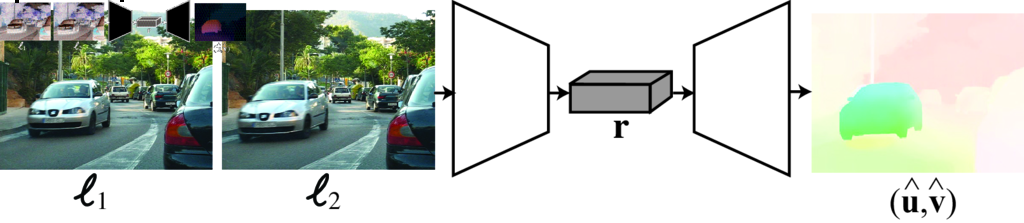
\includegraphics[width=.8\linewidth]{figures/optical_flow/supervised_estimation.eps}}
    \caption{In FlowNet the direct approach estimates optical flow directly from a pair of frames.}
    \label{fig:supervised_estimation}
\end{figure}
\vspace{-.2in}
The direct approach depicted in \fig{\ref{fig:supervised_estimation}} learns to estimate optical flow directly from a pair of frames. This architecture makes no assumptions about which architectural priors are needed to compute optical flow from images. The architecture is trained end-to-end using ground truth optical flow.

Another common approach, depicted in the block diagram shown in \fig{\ref{fig:supervised_estimation_modular}}, is to define an architecture that follows the same steps as traditional approaches:

\begin{itemize}
    \item Extract features from each image using a pair of networks with shared weights. This can be done by a feature pyramid \cite{Lin2017}.
    \item Form a 3D cost volume indicating the local visual evidence of a match between the two images for each possible pixel position. This 3D cost volume can be referenced to the $H$ and $V$ positions of one of the input images (generally the first frame is the reference frame).
    \item Train and apply a CNN to aggregate (process) the costs over the  cost volume in order to estimate a single best optical flow for each pixel position.
    \item Use a coarse-to-fine estimation procedure where optical flow estimated at a coarse scale is used to warp the features at a finer scale to compute a refined cost volume. Then, estimate an update to the optical flow to warp the features and the next finer level of the pyramid.
\end{itemize}

\vspace{-.2in}
\begin{figure}[h!]
    \centerline{
        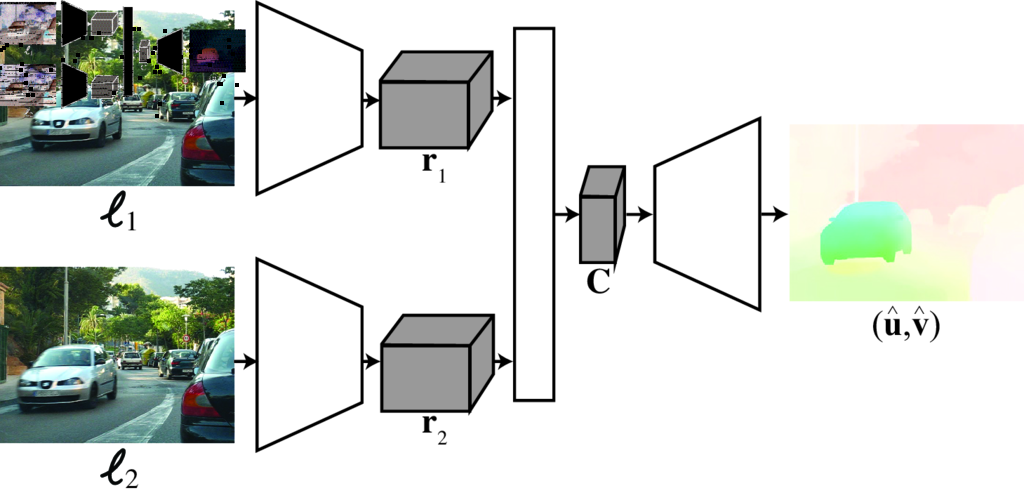
\includegraphics[width=.8\linewidth]{figures/optical_flow/supervised_estimation_modular.eps}}
    \caption{Motion estimation. (1) Extract
        features from each image;
        (2) compute a 3D cost volume;
        and (3) aggregate the
        cost volume in order to
        estimate the best optical
        flow for each pixel.
        %Motion estimation by: 1) Extract features from each image, 2) compute a 3D cost volume, and 3) aggregate the cost volume in order to estimate the best optical flow for each pixel.
    }
    \label{fig:supervised_estimation_modular}
\end{figure}


Other variations over this architecture incorporate some of the concepts we studied before, such as coarse-to-fine refinement, matching, and smoothing. Different approaches will differ in some of the details of how each step is implemented and how training takes place. The main building blocks can be implemented with convolutional neural networks or transformers.
The main difference between the matching-based and gradient-based methods described earlier is that instead of using predefined functions, the architectures are trained end-to-end to minimize the optical flow error when compared with ground truth data.


\subsubsection{Loss functions}
%~\\
In supervised optical flow estimation, the most common loss is the {\bf endpoint error},
\index{Endpoint error}
which is the average, over the whole image, if the distance between the estimated optical flow vector, $(\hat{u},\hat{v})$ and the ground-truth vector, $(u,v)$:
\begin{equation}
    \mathcal{L} \left( \hat{\mathbf{u}}, \hat{\mathbf{v}}, \mathbf{u}, \mathbf{v} \right) =
    \sum_{n,m} (\hat{u}[n,m] - u[n,m])^2 + (\hat{v}[n,m] - v[n,m])^2
\end{equation}
\marginnote{
    \centerline{
        \includegraphics[width=.3\linewidth]{figures/optical_flow/endpoint_error.eps}
    }
}
The sum is over all the pixels in the image. Each pixel has an estimated optical flow $(\hat{u}[n,m],\hat{v}[n,m])$.

\subsubsection{Handling occlusions}
%~\\
One of the challenges for estimating optical flow is that, as objects move, they will occlude some pixels from the background and reveal new ones. Therefore, together with the estimated flow it is also convenient to detect occluded pixels. If we have ground truth data, we can train a function to estimate optical flow and the occlusion map from two frames:
\begin{equation}
    \left[ \hat{\mathbf{u}}, \hat{\mathbf{v}}, \hat{\mathbf{o}} \right] =
    h_\theta \left( \boldimg_1, \boldimg_2 \right)
\end{equation}

\subsubsection{Training set}
%~\\
The biggest challenge of using a supervised model for motion estimation is that ground truth data is very hard to collect. This is probably one of the main limitations of these approaches. There are some small existing datasets, although this might change in a few years.

The largest existing datasets are synthetic 3D scenes with moving objects that can be rendered, which will give us perfect ground truth data to train the regression function. There are several examples of existing datasets such as this, like the Middelbury dataset \cite{Scharstein2002}, which contains six real and synthetic sequences with ground truth optical flow. The optical flow for the real sequences was obtained by tracking hidden fluorescent texture.
The KITTI dataset \cite{Geiger2013} contains real motion recorded from a moving car. The MPI Sintel \cite{Butler:ECCV:2012} contains synthetic sequences made with great effort to make the scenes look realistic. Finally, the Flying Chairs dataset is an interesting synthetic dataset that consists of pasting the image of a random number of chairs over a background image \cite{Dosovitskiy2015}. Motion is created by applying different affine transformations to the background and the chairs. These sequences are easy to generate and pay little attention to their realism. This makes it possible to generate a very large number of sequences for training, allowing for competitive performance when used to train a neural network.
% https://openaccess.thecvf.com/content_cvpr_2017/papers/Ilg_FlowNet_2.0_Evolution_CVPR_2017_paper.pdf

%\subsubsection{Evaluation}



%\subsubsection{Shortcomings}

%What happens to pixels that are only visible in one frame?

%This model does not make explicit additional restrictions such as a moving camera, or motion of rigid object. It might be that the internal representation learns to identify camera motion and to recognize specif objects with rigid motion or with restricted motion (such as objects moving on the ground such as cars). 

\subsection{Unsupervised Learning of Optical Flow}

Collecting ground truth data is the Achilles heel for learning-based approaches. This is particularly true for optical flow as it can not be recorded directly. Ground truth data optical flow can be obtained on synthetic data only, and for real data one needs to create specific recording scenarios that allow inferring accurate optical flow or relying on noisy human annotations \cite{Liu2008}. As a consequence, real data collection is expensive and nonscalable.

Is it possible to learn to estimate optical flow by just looking at movies without using ground truth data?

Unsupervised methods for training an optical flow model will make some assumptions about dynamic image formation. Those assumptions will be similar to the ones we have presented all along this chapter: (1) when the motion is due only to camera motion, the optical flow will have to fit the equations of the projected motion that provide constraints that can be used to train a model; (2) we can assume that the appearances of objects and surfaces in the scene do not change due to motion (brightness constancy assumption); and (3) we can expect the optical flow to be smooth over regions, although with sharp variations along occlusion boundaries.

One typical formulation consists in learning to predict the displacement from frame 1 to frame 2, so that if we warp frame 1 we minimize the reconstruction error of frame 2. This is achieved by using the photometric loss:

\begin{equation}
    L_{photo}(\boldimg_1,\boldimg_2,\mathbf{u}, \mathbf{v})=
    \sum_{x,y} \left| \img_2 (x+\hat{u},y+\hat{v}) - \img_1 (x,y)) \right| ^2
\end{equation}
where now $\left[ \hat{\mathbf{u}}, \hat{\mathbf{v}} \right] =  h_\theta \left( \boldimg_1, \boldimg_2 \right)$.

The learning is done by searching over the parameter space for the parameters $\theta$ that minimize the photometric loss over a large collection of videos. The photometric loss can also be replaced by the L1 or other robust norms. If the network also predicts occlusions, the photometric loss can include a weight that cancels the contribution of occluded pixels to the loss.

The network can also take as input multiple frames and not just two.



\section{Concluding Remarks}

Supervised and unsupervised learning-based methods are now the state-of-the-art in motion estimation. But an accurate solution is still missing. One important question is, do we really need learning in order to solve this problem? Should we abandon the derivation of physically motivated algorithms for motion estimation that require no training? Our answer is that we should pursue both directions of work.
  % antonio 
% 
%% jan. 4, 2011  items to fix:
%% notation for math and reference to images.
%% how include eps figures.
%% make all the little figures (search for eps) in a common, nice matlab way for the
%% example filtering operations.

%\setcounter{chapter}{5}
\chapter{Color}
\label{chapter:color}

%\reviewcomment{Figures need reformating.}

\section{Introduction}

There are many benefits to sensing color.  Color differences let us
check whether fruit is ripe, tell whether a child is sick by looking
at small changes in the color of the skin, and find objects in
clutter.  

We'll begin our study of color by describing the physical properties of light that lead to the perception of different colors.  Then we'll describe how humans and machines sense colors, and how to build a system to match the colors perceived by an observer.  We'll briefly describe how to represent color--different color coordinate systems.  Finally, we'll describe how spatial resolution and color interact.


\section{Color Physics}


Isaac Newton revealed several intrinsic
properties of light in experiments summarized by his drawing in
\fig{\ref{fig:prism}}. A pinhole of sunlight enters through the
window shade, and a lens focuses the light onto a prism.  The prism
then divides the white light into many different colors.  These
colors are elemental: if one of
the component colors is passed through a second prism, it doesn't
split into further components.


\begin{figure}[htpb!]
\centerline{
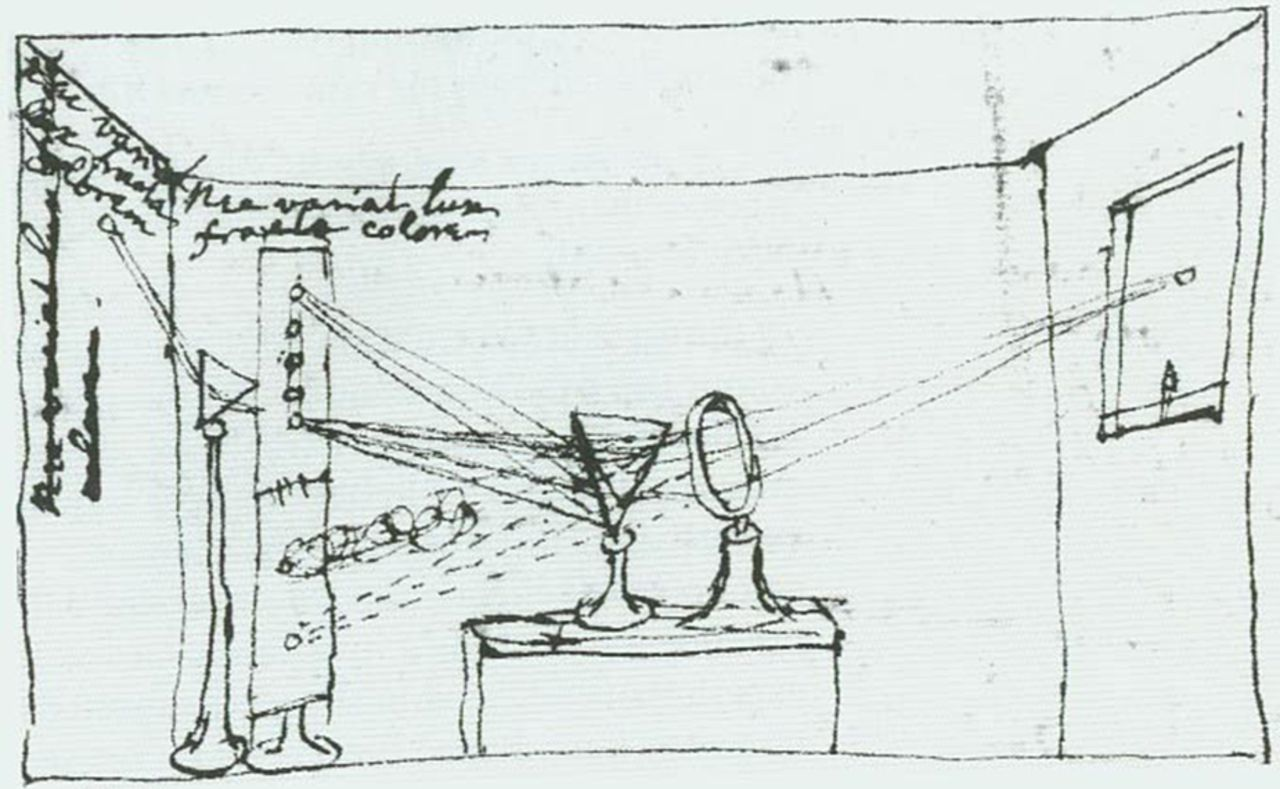
\includegraphics[width=.9\linewidth]{figures/color/newtonDrawing.jpg}
}
\caption{Isaac Newton's illustration of experiments with light \cite{Fara2015}.  White
light enters from a hole in the window shade at the right, where it is
focused with a lens and then passes through the first
prism.  The prism separates the white light into different colors by
bending each color a different amount.  The second prism in the
drawing demonstrates that those colors are elemental:  as an individual
color passes through the second prism, the light doesn't break into
other colors.}
\label{fig:prism}
\end{figure}


Our understanding of light and color explains such experiments.  Light
is a mixture of electromagnetic waves of different wavelengths.
Sunlight has a broad distribution of
light of the visible wavelengths.  At an air/glass interface, light
bends in a wavelength-dependent manner, so a prism disperses the
different wavelength components of sunlight into different angles, and
we see different wavelengths of light as different colors.  
Our eyes are sensitive to only the narrow band of that electromagnetic
spectrum, the visible light, from approximately 400 nm 
to 700 nm, which appears blue to deep red, respectively.




The bending of light at a material boundary is called {\bf refraction}, and
its wavelength dependence lets the prism separate white light into its
component colors.  A second way to separate light into its spectral
components is through {\bf diffraction}, where constructive
interference of scattered light occurs in different directions for
different wavelengths of light. 
\marginnote{Newton understood that white light could be decomposed into different colors and invented the term {\bf spectrum}.}

\Fig{\ref{fig:colorWavelengths}}{a} 
shows a simple spectrograph, an apparatus to reveal the spectrum of light, based on
diffraction from a compact disk (CD) \cite{spectrometer}.  Light passes through the slit at
the right, and strikes a CD (with a track pitch of about 1,600 nm).
Constructive interference from the light waves striking the CD tracks
will occur at a different angle for each wavelength of the light, yielding
a separation of the different wavelengths of light according to their
angle of diffraction.  The diffracted 
light can be viewed,   \fig{\ref{fig:colorWavelengths}}{b}, 
or photographed through the hole at the bottom
left of the photograph.  The spectrograph gives an immediate visual
representation of the spectral components of colors in the world. Some examples are shown in \fig{\ref{fig:examples1}}.



\begin{figure}[t]
\centerline{
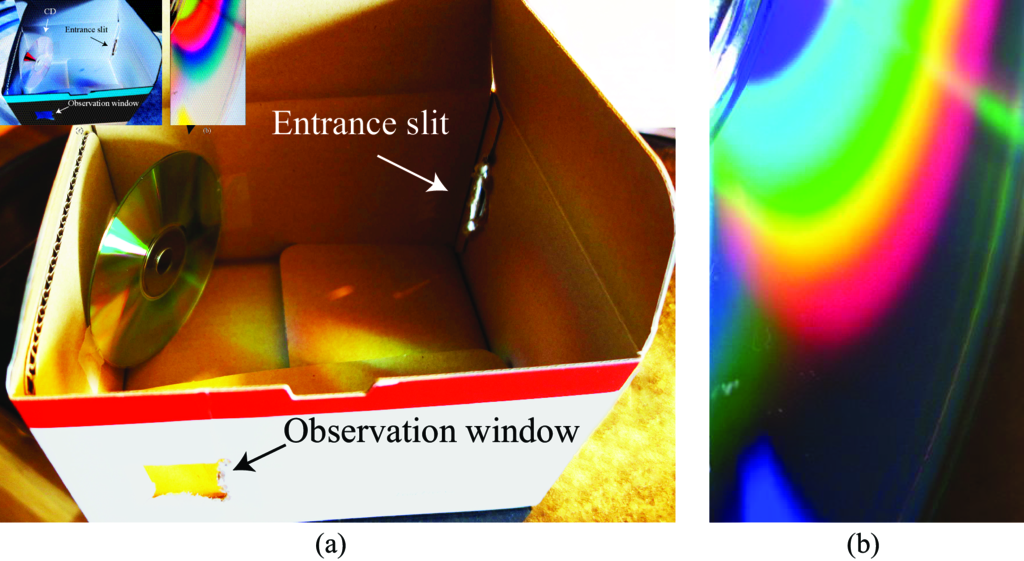
\includegraphics[width=1.0\linewidth]{figures/color/cd_spectrometer_setup.eps}
}
%\centerline{
%\sublabel{a}{\epsfig{file=figures/color/cdSpectrograph.eps,width=3in}}
%\sublabel{a}{\epsfig{file=figures/color/spectrometer2.jpg,width=3in}}
%\sublabel{b}{\epsfig{file=figures/color/rainbow.eps,width=1.5in}}}
\caption{(a) A simple spectrograph.
  Slit at right accepts light from primarily one object in the world.
  Light diffracted by the CD is viewed from the hole at the bottom
  left.  (b) The bending by diffraction is wavelength dependent, and the
  light from a given direction is broken into its spectral components. We indicate the location of the CD in the picture just in case our youngest readers have not seen one.}
\label{fig:colorWavelengths}
\end{figure}




\begin{figure}
\centerline{
\includegraphics[width=1.0\linewidth]{figures/color/lightspectra_objects.eps}
}
%\sublabel{a}{\centerline{
%\epsfig{file=figures/color/DSC00780.jpg,width=1.7in}
%\epsfig{file=figures/color/leafspec.eps,width=1.05in}
%}}
%\sublabel{b}{\centerline{
%\epsfig{file=figures/color/reddoor.eps,width=1.3in}
%\epsfig{file=figures/color/reddoorspec.eps,width=1.6in}
%}}
%\sublabel{c}{\centerline{
%\epsfig{file=figures/color/fourlamp.eps,width=1.7in}
%\epsfig{file=figures/color/neon.eps,width=1.5in}}}
\caption{The light spectra from some everyday objects, analyzed by the spectrograph of
  \fig{\ref{fig:colorWavelengths}}.  (a) A leaf, with some
  yellowish highlights, shows primarily green, with a little red (red
  and green can combine to appear yellow).  (b) A
  red door.  (c)  A fluorescent light (when turned on) shows the discrete spectral wavelengths at
  which the gas fluoresces.
}
\label{fig:examples1}
\end{figure} 


\subsection{Light Power Spectra}

The light intensity at each wavelength is called the {\bf power spectrum} of the
light.  The color appearance of light is determined by many factors, including the image context in which the light is viewed; but a very important factor in determining color appearance is the power spectrum. In this initial discussion of color, we will assume that the power spectrum of light determines its appearance, although you should remember that this is true only within a fixed visual context.

\marginnote{Why does the sky look blue? And why does it look orange during a sunset? 
\\[6pt]
\centerline{
\includegraphics[width=.4\linewidth]{figures/color/sunset_key_west.jpg}
}
}[-1.6in]

\Fig{\ref{fig:examples1}} shows a spectrograph visualization of some light power spectra (the right image of each row) along with the image that the spectrograph was pointed toward (left images).
\Fig{\ref{fig:sources}} shows the spectrum of a blue sky, plotted as 
intensity as a function of wavelength.



\begin{figure}
\centerline{
\includegraphics[width=0.7\linewidth]{figures/color/Spectrum_of_blue_sky.eps}
%\epsfig{file=figures/color/blueSky.jpg,width=3in}
~~~~~
\includegraphics[width=.15\linewidth]{figures/color/IMG_0122.jpg}
}
\caption{Power spectrum of blue skylight \cite{blueskyWiki}.}
\label{fig:sources}
\end{figure}


\subsection{The Color Appearance of Different Spectral Bands}

It is helpful to develop a feel for the approximate color appearance of different
light spectra.  Again, we say the approximate appearance because the subjective appearance can change according to other factors than just the spectrum.

The visible spectrum lies roughly in the range between 400 and 700 nm,
see \fig{\ref{fig:rainbow}}.  We can divide the visible spectrum into
three 100 nm bands, and study the appearance of light power
spectra where power is present or absent from each of those three
bands, in all of the eight ($2^3$) possible combinations.


\begin{figure}
\centerline{
\epsfig{file=figures/color/rainbow3.eps,width=5in}}
\caption{The approximate color appearance of light over different
  spectral regions.}
\label{fig:rainbow}
\end{figure}

Light with spectral power distributed in just the 400--500 nm
wavelength band will look some shade of blue, the exact hue depending
on the precise distribution.  Light in the 500--600 nm band will
appear greenish.  Most distributions within the 600--700 nm band will
look red.

White light is a mixture of all spectral colors.  A spectrum of light
containing power evenly distributed over 400---700 nm would appear approximately
white.  Light with no power in any of those three bands, that is, 
darkness, appears black.

There are three other spectral classes left in this simplified grouping
of spectra:  spectral power present in two of the spectral
bands, but missing in the third.
Cyan is a combination of both blue and green, or roughly spectral
power between 400 and 600 nm.  In printing and color film
applications, this is sometimes called {\em minus red}, since it is the
spectrum of white light, minus the spectrum of red light.  The blue
and red color blocks, or light in the 400--500 nm band, and in the
600--700 nm band, is called magenta, or minus green.  Red and green together,
with spectral power from 500--700 nm, make yellow, or minus blue (\fig{\ref{fig:names}}). 

\begin{figure}
\centerline{
\includegraphics[width=1.0\linewidth]{figures/color/cartoonColor2.eps}
}
%\epsfig{file=figures/color/cartoonColor2.eps,width=5in}}
\caption{For coarse orientation only, this cartoon model gives the color appearance of different spectral bands of the spectrum of visible light.}
\label{fig:names}
\end{figure}



\subsection{Light Reflecting from Surfaces}

When light reflects off a surface, the power spectrum alters in ways that depend on the surface’s characteristics and geometry. These
changes in light allow us to perceive objects and surfaces by observing their influence on the reflected light.

The interaction between light and a surface can be quite complex. Reflections can be specular or diffuse, and the reflected
power spectrum may depend on the relative orientations of the incident
light, surface, and the observed reflected ray. In its full generality, the reflection of light from a surface is described by the
bidirectional reflectance distribution function (BRDF) \cite{Nicodemus1965,Matusik2002}.
For this discussion, we will focus on diffuse
surface reflections, where the power spectrum of the reflected light, $r(\lambda)$,
is proportional to the wavelength-by-wavelength product of the power
spectrum of the incident light, $\imgin (\lambda)$, and a {\bf reflectance
  spectrum}, $s(\lambda)$, of the surface:
\begin{equation}
r(\lambda) = k \imgin (\lambda) s(\lambda),
\end{equation}
where the proportionality constant $k$ depends on the reflection geometry.
This diffuse reflection model characterizes
most matte reflections.  Such wavelength-by-wavelength scaling
is also a good model for the spectral changes to light caused by transmission
through an attenuating filter.  The incident power spectrum is
then multiplied at each wavelength by the {\bf transmittance spectrum} of
the attenuating filter.

Some reflectance spectra of real-world surfaces are plotted in
\fig{\ref{fig:sourcerefl}}.  The flower {\em Hepatica Nobilis} (solid line) is blue, while {\em Pyrostegia venusta} (dotted line) is orange.

\begin{figure}[t]
\centerline{
\includegraphics[width=1.0\linewidth]{figures/color/flowerSpectra.eps}
}
%\centerline{
%\sublabelnp{(a) reflectance functions of two flowers}{\epsfig{file=figures/color/flowerSpectra.jpg,width=3in}}
%\sublabelnp{(b) Hepatica nobilis (solid line)}{\epsfig{file=figures/color/nobilis.jpg,width=1.3in}}
%\sublabelnp{(c) Pyrostegia venusta (dotted line)}{\epsfig{file=figures/color/Pyrostegia_venusta3.jpg,width=1.3in}}
%}
\caption{Reflectance spectra from two flowers \cite{Arnold2010}. The blue {\em Hepatica nobilis} flower \cite{nobilis} and the orange flower, {\em Pyrostegia venusta} \cite{venusta}.}
\label{fig:sourcerefl}
\end{figure}




The reflectance spectrum of a surface often carries valuable information about the material being viewed, such as whether a fruit is ripe, whether a human's skin is healthy, or whether the material differs from another viewed material.  It may be the case that a low-dimensional version of the surface reflectance spectrum is sufficient for many visual tasks, and as we see subsequently, the human visual system represents color with only three numbers.  So it is an important visual task to estimate either the surface reflectance spectrum, or a low-dimensional summary of it. 


To estimate surface colors by looking, a vision system has the task of estimating the illumination spectrum and the surface reflectance spectra, from observations of only their products.
When the illumination is white light with equal power in all spectral bands,
the observed reflected spectrum is proportional to the reflectance spectrum of the
material itself.  However, under the more general condition of unknown illumination color, a visual system will need to estimate the surface reflectance spectrum, or projections of it, by taking the context of nearby image information into account.

There are many proposed algorithms to do that, ranging from heuristics, for example, assuming the color of the brightest observed object is white \cite{McCann76}, to statistical methods \cite{Brainard97} and neural network based approaches \cite{Barron2015}.
Even humans don't solve the problem perfectly or consistently, revealed especially through the internet meme of \#TheDress \cite{Bleasdale2015}, 
%``TheDress'', 
shown in \fig{\ref{fig:thedress}}.  


\begin{figure}[t]
\centerline{
%\sublabel{a}{\epsfig{file=figures/color/thephotoofthedress.jpg, width=1.9in}}
%\sublabel{b}{\epsfig{file=figures/color/gr2_lrg.jpg, width=2.9in}}
\sublabel{a}{\includegraphics[width=1.9in]{figures/color/thephotoofthedress.jpg}}
\sublabel{a}{\includegraphics[width=2.9in]{figures/color/gr2_lrg.jpg}}
}
\caption{(a) \#The Dress, photographed and posted by \cite{Bleasdale2015}, reprinted with permission.  (b) The spectra of the light we see is the product of an assumed illumination spectrum and the inferred surface reflectance spectra.  If people make different assumptions about the illumination, they can perceive different colors within the same image, as shown in this illustration \cite{Brainard2015}.  Reprinted with permission from Elsevier.
}
\label{fig:thedress}
\end{figure}



The perceived colors of the dress depend on the assumed color of the illumination, and people can disagree significantly about the colors they see \cite{Brainard2015}.  The assumption of a warm, yellowish, illumination color leads to a perception of blue and black material.  The assumption of a cool, blueish illumination leads to a perception of white and gold material.  Both perceptions are consistent with the observed product of illumination and reflectance  seen in the dress image.  

\marginnote{Did you perceive the dress, \fig{\ref{fig:thedress}}, to be black on blue, or gold on white?  Can you make the perception change?}

While such context-dependent effects are important in color perception, as we quantify color perception we will assume that our perception of color depends only on the spectrum of light entering the eye.  This will serve us well for many industrial applications.


\section{Color Perception}

Now we turn to our perception of color.  We first describe the
machinery of the eye, then describe some methods to measure color appearance.  These methods to measure color appearance implicitly assume a white illumination spectrum, but they often serve the needs of industry and science.


\subsection{The Machinery of the Eye}

%Figure~\ref{fig:ramon}~a is a drawing \cite{cajal1904} of the photoreceptors, called the rod and cones, in the retina of the eye.  The tall receptors are the rods, used in low-light levels, and the short ones are the cones, used in color vision.  Interestingly, the light enters from the bottom of the drawing, passing through the nerve fibers and blood vessels before reaching the photosensitive detectors at the top of the image. 



An instrument such as a spectrograph (\fig{\ref{fig:colorWavelengths}} shows a simple one)
can measure the light power spectrum at hundreds of
different wavelengths within the visible band, yielding hundreds of
numbers to describe the light power spectrum.  Despite this, a useful
description of the visual world can be obtained from a much lower
dimensional description of the light power spectrum.  
\marginnote{The retina contains photoreceptors called the rod and cones. Rods are used in low-light levels, and the cones are used in color vision. In low-light, only the rods operate and our vision becomes black and white.}

The human visual
system analyzes the incident light power spectrum with only three
different classes photoreceptors, called the L, M, and S cones because
they sample at the long, medium, and short wavelengths.  This gives
the human visual system a three-dimensional (3D) description of light, with
each photoreceptor class taking a different weighted average of the
incident light power spectrum.

\Fig{\ref{fig:ramon}}{a} shows 
the spatial sampling pattern, for each of the three cone classes, measured from a subject's eye \cite{Hofer2005}. The L cones are
colored red, the M cones green, and the S cones are colored
blue. Note the hexagonal packing of the cones in the retina, and the
stochastic assignment of L, M, and S cones over space.  Note also the much sparser spatial sampling of the S cones than of either the L or M cones.
\Fig{\ref{fig:ramon}}{b} shows the spectral sensitivity curves
for the L, M, and S cones.  This sampling pattern was measured from near the {\bf fovea}, where there are no rods, and the cones are close-packed.


\begin{figure}[t]
\centerline{
%\sublabel{a}{\epsfig{file=figures/color/ramonycajal,width=2in}}
\sublabel{a}{\epsfig{file=figures/color/YYretina.pdf,width=2in}}
\sublabel{b}{\epsfig{file=figures/color/Cones_SMJ2_E.jpg,width=2.5in}}
}
%\centerline{
%\sublabel{c}{\epsfig{file=figures/color/Cones_SMJ2_E.jpg,width=4in}}
%}
\caption{
%(a) Drawing of the eye's photoreceptors by the physiologist Ramon y Cajal \cite{cajal1904}.
 (a)  Measured cone receptor classes and positions in a human retina, with cone receptor classes shown as red, green, and blue (subject YY, redrawn from \cite{Hofer2005}).
(b) Photoreceptor sensitivities as a function of light wavelength  \cite{Vanessaezekowitz2007}.}
\label{fig:ramon}
\end{figure}


We can describe the photoreceptor responses using matrix algebra.
If the matrix $\mathbf{C}_{\mbox{eye}}$ consists of the spectral sensitivities of the
L, M, and S cones in three rows, and the vector $\mathbf{t}$ is a column
vector of the spectrum of light incident on the eye, then the L, M,
and S cone responses will be the product,
\begin{equation}
    \begin{bmatrix}
    L  \\
    M  \\
    S \\
    \end{bmatrix}
= \mathbf{C}_{\mbox{eye}} \, \mathbf{t}
\label{eq:lmsct}
\end{equation}

The fact that our eyes have three different classes of photoreceptors
has many consequences for color science.  It determines that there are
three primary colors, three color layers in photographic film, and
three colors of dots needed to render color on a display screen.  In
the next section, we describe how to build a color reproduction system that matches the colors seen in the world by a human observer.

%% \billf{Who first discovered trichromaticity, and how?}


\subsection{Color Matching}

Color science tells us how to analyze and reproduce color.
We seek to build image displays so that the output colors match those of
some desired target, and to manufacture items with the same colors over
time.  Much of the color industry revolves around the ability to repeatably control colors.
Colors can be trademarked (Kodak Yellow, IBM Blue) and we have
color standards for foods.  \Fig{\ref{fig:french}} shows French fry color
standards.

\begin{figure}[t]
\centerline{
\epsfig{file=figures/color/munsell.jpg,width=3.5in}}
\caption{The USDA color standards for French fried potatoes, one of
  many color standards \cite{Munsell2020}.} 
\label{fig:french}
\end{figure}

One of the tasks of color science is to predict when a person will
perceive that two colors match.  For example, we
want to know how to adjust a display to match the color
reflecting off some colored surface.  Even though the spectra may be
very different, the colors can almost always be made to match.

It is possible to infer human color matching performance by examining the spectral sensitivity curves of the receptors shown in \fig{\ref{fig:ramon}}{b}. We attempt to match a color using a combination of reference colors, typically called primary colors. Through experimentation, it has been discovered that the appearance of any color can be matched through a linear combination of three primary colors. This is due to the presence of three classes of photoreceptors in our eyes. It has also been found that these color matches are transitive—if color A matches a particular combination of primaries and color B matches the same combination of primaries, then color A will match color B. Consequently, the amount of each primary required to match a color can serve as a set of coordinates indicating color \cite{Wandell95}.

\subsection{Color Metamerism}


Two different spectra are metameric if they appear to be the same color to our eyes.
There is a large space of metamers:  any two 
vectors describing light power spectra
that give the same projection onto a set of color matching functions
will look the same to our eyes.  There's a high-dimensional space of light spectra, and we're
only viewing projections onto a 3D subspace in the colors we see.\marginnote{Do spotlights on produce in a supermarket help good and bad fruit become metameric matches?}

In practice, the three projections we observe capture much of the interesting action in images.  Hyperspectral images (recorded at many different wavelengths of analysis) add some, but not
a lot, to the image formed by our eyes.



\subsection{Linear Algebraic Interpretation of Color Matching}


% \begin{figure}
% \centerline{
%\epsfig{file=figures/color/conditions.jpg,width=4in}
%\epsfig{file=figures/color/conditionsForMatch.jpg,width=4in}
% }
% \caption{Conditions for a perceptual match for the system of Fig.~\ref{fig:colorsystem}.  First, $\mathbf{C}$ must be a linear combination of the spectral sensitivities of the photoreceptors in the eye, thus $\mathbf{C} = \mathbf{R} \mathbf{C}_{\mbox{eye}}$, for some full-rank, 3x3 matrix, $\mathbf{R}$.  Second, the light sensor spectra, in the rows of $\mathbf{C}$, and the display element spectra, in the columns of $\mathbf{P}$, must satisfy $\mathbf{C}\mathbf{P} = \mathbf{I}_{\mbox{3}}$.}
% \label{fig:conditions}
% \end{figure}

In this chapter, we assume that color appearance is determined by the light spectrum reaching the eye. In reality, numerous factors can influence color appearance, including the eye's state of brightness adaptation, ambient illumination, and surrounding colors. However, a color matching system that relies solely on the light spectrum will still perform well.

To measure the color associated with a light spectrum $\mathbf{t}$ we need to be able to predict the eye's responses to the spectrum.
From \eqn{\ref{eq:lmsct}}, the task of color measurement is to find the projection of a given light spectrum into the
special 3D subspace defined by the eye's cone spectral response curves.
Any basis for that 3D subspace will serve that task, so the three basis
functions do not need to be the color sensitivity curves of
\fig{\ref{fig:ramon}} themselves.  They can be any linear combination
of them, as well. 

We can define a {\bf color reproduction system}, \fig{\ref{fig:colorsystem}}, by first specifying its  three spectral sensitivity curves.  We put these into the $3 \times N$ matrix, $\mathbf{C}$, where $N$ is the number of spectral samples over the visible illumination range.  As discussed previously, the three curves, $\mathbf{C}$, should be a linear combination of the eye's spectral sensitivity curves, or
\begin{equation}
    \mathbf{C} = \mathbf{R} \, \mathbf{C}_{\mbox{eye}},
    \label{eq:match2}
\end{equation}
where $\mathbf{R}$ is any full-rank $3 \times 3$ matrix. We can translate between any two different color
spaces by  applying a general $3 \times 3$ matrix transformation
to change basis vectors.  Note, the basis vectors do not need to be
orthogonal, and  most color system basis vectors are not.


\begin{figure}[t]
\centerline{
\includegraphics[width=1.0\linewidth]{figures/color/colorRepro2.pdf}
}
%\centerline{
%% \epsfig{file=figures/color/colorsystem.jpg,width=5in}}
%\epsfig{file=figures/color/colorRepro.jpg,width=5in}}
\caption{A color reproduction system.  Light sensors a, b, and c respond to the input light spectrum $\mathbf{t}$, giving sensor activations $\mathbf{C} \mathbf{t}$.  Combinations of those activations drive the display elements d, e, and f, producing the output spectrum $\mathbf{P}\mathbf{M} \mathbf{C} \mathbf{t}$. Conditions on $\mathbf{P}$, $\mathbf{M}$, and $\mathbf{C}$ can ensure that the input and output colors match for an observer.}
\label{fig:colorsystem}
\end{figure}


\subsection{Color Matching Functions and Primary Lights}

A  color reproduction system measures an input light and produces an output light that matches the color appearance of the input light.  A camera with a screen display is an example of a color reproduction system, as the colors of objects in the world are measured, then reproduced on the screen display of the camera.  
We can match the eye's response to a given light spectrum through the appropriate control of a sum of three lights, which we'll call the {\bf primary lights}\index{Color!Primary colors}. For the example of a display screen, the three color elements of each pixel are the primary lights.  

Because the eye's photosensors respond in linear proportion to the amount of the incoming light spectrum within its spectral sensitivity curve, the rules of linear algebra apply to color manipulation.  For a given set of three primary lights, the strengths of each primary light can be adjusted to obtain a visual match to a desired color.  There is one exception to this: because primary lights can only be combined in positive values, some input colors are outside the {\bf gamut}---the range of colors that can be produced---of a the positive combination of a given set of primary lights.

The color reproduction system is then defined by two sets of spectral curves and a $3 \times 3$ matrix, $\mathbf{M}$, see \fig{\ref{fig:colorsystem}}.  The first set are the spectral sensitivities as a function of wavelength for each of the three photosensors.  We write each of those spectral curves as a row vector of a matrix, $\mathbf{C}$.  The $3 \times 3$ matrix, $\mathbf{M}$, translates any color measurement to a set of amplitude controls for the primary lights, $\mathbf{P}$. The second set of spectral curves of a color reproduction system are the spectra of the three primary lights, which we write as column vectors of the matrix, $\mathbf{P}$.

For a given set of primary lights, $\mathbf{P}$, we seek to find a matrix of color sensitivity curves, $\mathbf{C}$, and $3 \times 3$ matrix, $\mathbf{M}$, which allow perfect reproduction of colors, as viewed by a human observer.  Here, we derive the conditions
%, given in \fig{\ref{eq:conditions}}, 
that $\mathbf{P}$,  $\mathbf{C}$, and $\mathbf{M}$ must satisfy to allow for perfect reproduction of colors.

Let the spectrum of the light reflecting from the surface to be matched in color be $\mathbf{t}$.  The eye's response to that light is modeled as the sum of a term-by-term multiplication of the spectral sensitivities of each photoreceptor, in the rows of $\mathbf{C}_{\mbox{eye}}$ times the spectrum of the light.  Thus, the responses of the eye to that spectrum will be the $3 \times 1$ column vector, $\mathbf{C}_{\mbox{eye}} \mathbf{t}$.  

We can write the response of the eye to the {\em output} of the color matching system as the following matrix products.  The light impinging on the sensors (a, b, c in \fig{\ref{fig:colorsystem}}) of the color matching system will give responses $\mathbf{C} \mathbf{t}$ and controls  $\mathbf{M} \mathbf{C} \mathbf{t}$ to the primary lights.  If this output modulates the corresponding primary lights (d, e, and f in \fig{\ref{fig:colorsystem}}), then the light displayed by the color matching system will be $\mathbf{P} \mathbf{M} \mathbf{C} \mathbf{t}$.  We want this spectrum to give the same responses in the eye as the original reflected color, thus we must have:
$\mathbf{C}_{eye} \mathbf{P} \mathbf{M} \mathbf{C} \mathbf{t} = \mathbf{C}_{eye} \mathbf{t} $.  Because that relation must hold for {\em any} input vector $\mathbf{t}$, we must have
\begin{equation}
\mathbf{C}_{eye} \mathbf{P} \mathbf{M} \mathbf{C}  = \mathbf{C}_{eye}   
\label{eq:match}
\end{equation}

What conditions on $\mathbf{P}$ and $\mathbf{C}$ are required for \eqn{\ref{eq:match}} to hold?  First, the subspace of the eye responses $\mathbf{C}_{eye}$ must be the same as that measured by the color sensing system, $\mathbf{C}$.  If that weren't the case, 
then perceptibly different spectra could map onto the same color sensing system measurements. So we must have $\mathbf{C} = \mathbf{R} \mathbf{C}_{eye}$, for some full-rank $3 \times 3$ matrix, $\mathbf{R}$ (with inverse $\mathbf{R}^{-1}$).  Substituting this twice into \eqn{\ref{eq:match}} gives
\begin{equation}
\mathbf{R}^{-1} \mathbf{C} \mathbf{P} \mathbf{M} \mathbf{R} \mathbf{C}_{eye} = \mathbf{C}_{eye}
\label{eq:match2}
\end{equation}
From \eqn{\ref{eq:match2}} it follows that  $\mathbf{C} \mathbf{P} \mathbf{M} = \mathbf{I}_3$, the $3 \times 3$ identity matrix.  These conditions on the spectral sensitivities, $\mathbf{C}$, the display spectra, $\mathbf{P}$ and the sensors-to-primaries mixing matrix, $\mathbf{M}$ for a color reproduction system are  summarized below:
\begin{eqnarray}
\mathbf{C} & = & \mathbf{R} \mathbf{C}_{\mbox{eye}} 
\label{eq:conditionsA} \\
\mathbf{M} & = & (\mathbf{C P})^{-1},
\label{eq:conditions}
\end{eqnarray}
where $\mathbf{C}_{\mbox{eye}}$ are the human photoreceptor sensitivities and $\mathbf{R}$ is a full-rank $3 \times 3$ matrix.  

%\marginnote{Conditions required for color matching in the color reproduction system of \fig{\ref{fig:colorsystem}}.}

\Fig{\ref{fig:exampleColor}} displays  the elements of two matrices $\mathbf{C}$ and $\mathbf{P}$ that define a valid color matching system.  For a color reproduction system to be physically realizable, the elements of the primary spectra, $\mathbf{P}$, must be non-negative.

% (In some color reproduction systems, there
% may be an additional 3x3 matrix Q multiplying the raw sensor spectral sensitivities to obtain the 
% color matching matrix C).



\begin{figure}[t]
\centerline{
\sublabelnp{(a)}{\epsfig{file=figures/color/ciergb.jpg,width=2.5in}}
\sublabelnp{(b)}{\epsfig{file=figures/color/primaryLights.jpg,width=2.5in}}}
\caption{The elements of the matrices $\mathbf{C}$ and $\mathbf{P}$ for an example color matching system.  (a) Spectral sensitivity curves, the rows of a color measurement matrix, $\mathbf{C}$. These should be linear combinations of the eye's photosensitivity curves, $\mathbf{C}_{\mbox{eye}}$.
(b) Corresponding primary lights, $\mathbf{P}$ \cite{Acdx2009},  satisfying $\mathbf{C} \mathbf{P}= \mathbf{I}_3$ ($\mathbf{M} = \mathbf{I}_3$  in equation [\ref{eq:conditions}]).}
\label{fig:exampleColor}
\end{figure}

Because many color sensitivity matrices $\mathbf{C}$ can satisfy \eqn{\ref{eq:conditionsA}} some standardized color sensitivity matrices have been adopted to allow common representations of colors. 


\subsection{CIE Color Space}

A color space is defined by the matrix, $\mathbf{C}$, with three rows
of color sensitivity functions.  These three sensitivity functions, $\mathbf{C}$, must be some linear combination of the sensitivity functions of the eye, $\mathbf{C}_{\mbox{eye}}$.
One color standard is the Commission Internationale de l'Eclairage (CIE) {\em XYZ} color space, $C_{\mbox{CIE}}$.  The CIE color matching functions, the rows of $\mathbf{C}_{\mbox{CIE}}$
were designed to be all-positive at every wavelength and are shown
in \fig{\ref{fig:ciecie}}.  


\begin{figure}[t]
\centerline{
{\epsfig{file=figures/color/ciecie.jpg,width=3in}}}
\caption{CIE color matching functions \cite{cie1931}.}
\label{fig:ciecie}
\end{figure}


An unfortunate property of the CIE color-matching functions is that no all-positive set of color primaries, $\mathbf{P}_{\mbox{CIE}}$ forms a color-matching system with those color-matching functions, $\mathbf{C}_{\mbox{CIE}}$.  But $\mathbf{C}_{\mbox{CIE}}$ is a valid matrix with which to measure colors, even though there is no physically realizable set of corresponding color primaries, $\mathbf{P}_{\mbox{CIE}}$.

To find the CIE color coordinates, one projects the input spectrum
onto the three color-matching functions, to find coordinates, called
tristimulus values, labeled $X$, $Y$, and $Z$.   Often, these values are
normalized to remove overall intensity variations, and one calculates {\bf CIE chromaticity coordinates}\index{Color!CIE chromaticity coordinates} $x = \frac{X}{X+Y+Z}$ and $y = \frac{Y}{X+Y+Z}$.



\begin{comment}
\begin{figure}[htpb!]
\centerline{
\epsfig{file=figures/color/metamerism.eps,width=6in}}
\caption{The two spectra in the figure above, from \cite{Wandell95},
  are colors that match perceptually:  daylight, and the spectrum a
  monitor adjusted to match daylight.    The figure at right shows a
  graphical rendition of the projection from the high-dimensional
  space of power spectra onto a lower-dimensional subspace,
  representing the 3D space of human color perception.  The red and
  blue dots in the higher-dimensional space are ``metameric'' in that
  they project to the same location in the lower-dimensional subspace.}
\label{fig:metamerism}
\end{figure}
\end{comment}

\begin{comment}
Let us summarize our discussion of color so far.  Under certain
viewing conditions, the perceived color depends just on the spectral
composition of light arriving at the eye (we move to more general
viewing conditions next).  Under such conditions, there is a simple
way to describe the perceived color:  project its power spectrum onto
a set of 3 vectors called color matching functions.  These projections
are the color coordinates.  
We standardize on particular sets of color coordinates.  One such set
is the CIE XYZ system.  
\end{comment}

\begin{comment}
How do you translate from one set of color coordinates
to another, say, for notation, from the color coordinates in a unprimed system to those
in a primed system?   Place the spectra of a set of primary lights
into the columns of a matrix ${\bf P}$.  If we take the color
coordinates, $\mathbf{x}$, as a 3x1 column vector and multiply them by the matrix
${\bf P}$, we get a spectrum which is metameric with the input
spectrum whose color coordinates were $\mathbf{x}$.  So to convert
$\mathbf{x}$ to its representation in a primed coordinate system, we just
have to multiply this metameric spectrum by  the color matching
functions for the primed color system:
\begin{equation}
\mathbf{x}' = {\bf C}'{\bf P} \mathbf{x}
\end{equation}
The color translation matrix ${\bf C}'{\bf P}$ is a 3x3 matrix.
\end{comment}



%% When did people learn that we have three color receptors, and how did
%% they find out?  ((   read about it.        ))



\begin{comment}

\subsection{Color mixing}

In art or photography, we often talk of ...      (relate to color primaries).


\begin{figure}[htpb!]
\centerline{
\epsfig{file=figures/color/yellowgreen.eps,width=1.5in}}
\caption{The cyan of Windex and the yellow of Joy combine to give a
 green color.}
\label{fig:colormixing}
\end{figure}

Colors and color mixing are a delightful aspect of our visual experience.
Fig.~\ref{fig:colormixing} shows an everyday example of color mixing:
yellow and cyan colors combining to give a green. 

Physically, color mixing involes combining the spectra of the two
colors to be mixed to create the power spectrum of the mixed color.
Various processes cause colors to mix, but the results
can be divided into two broad classes of mixing, called additive and
subtractive.  Under additive color mixing, the
power spectra add together to form the spectrum of the resulting
color.  This model of mixing covers the case of many small color 
elements for which the appearance is fused, such as tiny elements of a
display, or the case of several light projectors pointing at the same screen.
CRT color televisions, DLP projectors, and
colors viewed very closely in space or time all exhibit additive color
mixing.  The spectrum of the mixed color is a weighted sum of the
spectra of the individual components.  In the additive
color mixing model, red and green combine to give yellow, as can be
seen from the cartoon models of Figs.~\ref{fig:names} and
\ref{fig:colormixing}. 

A second way colors combine is called subtractive color mixing, but
might better be called multipliciative color mixing.  Under this
mixing model, the spectrum of the combined color is proportional to
the {\em product} of the mixed components.  This color mixing occurs
when light of one color reflects diffusely off a surface of another
color, or passes through a sequence of attenuating spectral filters,
such as with photographic film, paint, optical filters, and crayons.
Under the subtractive color mixing model, cyan and yellow combine to
give green, since the cyan filter attenuates the red components of
white light, and yellow filter would remove the remaining blue
components, leaving only the green spectral region of the original
white light.  Under subtractive color mixing,  red and green combine to give black.

Figure~\ref{fig:mixing} shows examples of color mixing.

\begin{figure}[htpb!]
\centerline{
\sublabel{a}{\epsfig{file=figures/color/additiveMixing.eps,width=3in}}
\sublabel{b}{\epsfig{file=figures/color/subtractiveMixing.eps,width=3in}}}
\caption{Examples of color mixing, in the world of cartoon color spectra.  (a) Additive, (b) subtractive.  The
 spectra and the resulting colors.}
\label{fig:mixing}
\end{figure}


Because the spectrum depends on surfaces, it is very useful to measure
the spectrum of reflected light, and we discuss how the eye does that
in the following section.

\end{comment}



\section{Spatial Resolution and Color}

Color interacts with our perception of spatial resolution.  For some directions in color space, the eye is very sensitive to fine spatial modulations, while for other color space directions, the eye is relatively insensitive.  Some color coordinate systems take advantage of this disparity to enable efficient representation of images by sampling image data sparsely along color axes where human perception is insensitive to blurring.

In a red-green-blue (RGB) representation, the eye is sensitive to high spatial frequency changes in both red and green, as shown in figures \ref{fig:girls1} and \ref{fig:girls2}.  A rotation of the color coordinates of the image, followed by a nonlinear stretching, can put the image into a color space called L, a, b\index{Color!Lab space}.  In that space, the eye is very sensitive to any blurring of the L color component, called luminance, but is relatively insensitive to blurring of the a or b components, as demonstrated in \fig{\ref{fig:girls3}} and \ref{fig:girls4}.  This effect is commonly exploited in image compression, allowing some image components to be sampled more coarsely than others.


\begin{figure}
\centerline{
\includegraphics[width=1.0\linewidth]{figures/color/nonblur_girls.eps}
}
%\centerline{
%\sublabelnp{(a) Original}{\epsfig{file=figures/color/nonblur.eps,width=2.3in}}
%\sublabelnp{(b) R, G, B components}{\epsfig{file=figures/color/rgbgirls.eps,width=2.3in}}
%\sublabelnp{(c) blurred R, G, B components}{\epsfig{file=figures/color/blurrgbgirls.eps,width=2.0in}}}
\caption{(a) Original image.  (b) RGB components.  (c) RGB components,
  each blurred.  These sharp and blurred components are used  in the color images of \fig{\ref{fig:girls2}}.
}
\label{fig:girls1}
\end{figure}



\begin{figure}
\centerline{
\includegraphics[width=1.0\linewidth]{figures/color/blur_rgb_girls.eps}
}
%\centerline{
%\sublabelnp{(a) R component blurred}{\epsfig{file=figures/color/blurrgirls.eps,width=2.3in}}
%\sublabelnp{(b) G component blurred}{\epsfig{file=figures/color/blurggirls.eps,width=2.3in}}
%\sublabelnp{(c) B component blurred}{\epsfig{file=figures/color/blurbgirls.eps,width=2.3in}}}
\caption{Color images composed of sharp and blurred components from figures \ref{fig:girls1}(b) and \ref{fig:girls1}(c).  (a) R component blurred, G and B components sharp.  (b)  G component blurred, R and B components sharp. (c) B component blurred, R and G components sharp. Blurring either the R or G components of the image leads to a blurry-looking full-color image.
}
\label{fig:girls2}
\end{figure}

\begin{comment}
\begin{figure}[htpb!]
\centerline{
\epsfig{file=figures/color/rgbyiq.eps,width=3in}}
\caption{Human spatial frequency sensitivity in R, G, B and L, a, b
  color representations
}
\label{fig:sensitivity}
\end{figure}
\end{comment}




\begin{figure}
\centerline{
\includegraphics[width=1.0\linewidth]{figures/color/nonblur_lab_girls.eps}
}
%\centerline{
%\sublabelnp{(a) Original}{\epsfig{file=figures/color/nonblur.eps,width=2.3in}}
%\sublabelnp{(b) L, a, b components}{\epsfig{file=figures/color/labgirls.eps,width=2.3in}}
%\sublabelnp{(c) blurred L, a, b components}{\epsfig{file=figures/color/blurlabgirls.eps,width=2.3in}}}
\caption{(a) Original image.  (b) Lab components.  (c) Lab components,
  each blurred.   These sharp and blurred components are used  in the color images of \fig{\ref{fig:girls4}}.
}
\label{fig:girls3}
\end{figure}



\begin{figure}
\centerline{
\includegraphics[width=1.0\linewidth]{figures/color/blur_lab_girls.eps}
}
%\centerline{
%\sublabelnp{(a) L component blurred}{\epsfig{file=figures/color/blurlgirls.eps,width=2.3in}}
%\sublabelnp{(b) a component blurred}{\epsfig{file=figures/color/bluragirls.eps,width=2.3in}}
%\sublabelnp{(c) b component blurred}{\epsfig{file=figures/color/blurbbgirls.eps,width=2.3in}}}
\caption{Color images composed of sharp and blurred components from figures \ref{fig:girls3}(b) and \ref{fig:girls3}(c).  (a) L component blurred, a and b components sharp.  (b)  a component blurred, L and b components sharp. 
(c) b component blurred, L and a components sharp. Blurring only either of the a or b components of the image yields a full-color image that appears sharp, provided the luminance component of the image is sharp.}
\label{fig:girls4}
\end{figure}





\begin{comment}

\subsection{Low-dimensional models for spectra}

Before we turn to color perception, let's introduce a mathematical
model for light spectra that makes them much easier to work with.  In
general, when modeling the world, we want to keep everything as simple
as possible, and that usually means working with as few degrees of freedom as
possible.   Color spectra seem like relatively high-dimensional
objects, since we can pick any combination of numbers, from 400 to 700
nm, as we'd like.  Even sampling at every 10 nm of wavelength, that
gives us 31 numbers for each spectrum.

It turns out that for many real-world spectra, those 31 numbers are not
independent and in practise spectra have far fewer degrees of freedom.
It is common to use low-dimensional linear models to approximate
real-world reflectance and illumination spectra.   Any given spectrum, say
$S(\lambda)$, is approximated as some linear combination of ``basis
spectra'', $u(\lambda)$.  For example, a 3-dimensional linear model of $S(\lambda)$
would be
\begin{equation} 
\left( 
\begin{array}{c}
\vdots \\
S(\lambda) \\
\vdots
\end{array}
\right) 
\approx
\left( 
\begin{array}{ccc}
\vdots  & \vdots & \vdots \\
u_1 (\lambda)  & u_2 (\lambda)  & u_3 (\lambda)  \\
\vdots & \vdots & \vdots 
\end{array}
\right) 
\left( 
\begin{array}{c}
\omega_1 \\
\omega_2 \\
\omega_3
\end{array}
\right) 
\label{eq:lowd}
\end{equation} 

The basis spectra can be found from a collection of training spectra.
If we write the training spectra as columns of a matrix, $D$, then
performing a singular value decomposition on $D$ yields
\begin{equation}
D = U * \Lambda * V'
\end{equation}
where $U$ is a set of orthonormal spectral basis vectors, $\Lambda$ is a
diagonal matrix of singular values, and $V'$ is a set of
coefficients.  The first $n$ columns of $U$ are the $n$ basis spectra that
can best approximate the spectra in the training set, in a least
squares sense.

Here's a demonstration, with a particular collection of
surface reflectance spectra, $u_i(\lambda)$ that this works quite well.  The ``Macbeth
Color Checker'', a tool of color scientists and engineers,
 is a standard set of 24 color tiles, made the same way year after
 year.  (So iconic that this woman, a dedicated color scientist, I
 presume, has tatooed a Macbeth color checker on her arm!  Alas, I'm
 sure the tatoo colors are only an approximation to the real Macbeth colors).

The reflectance spectra of each Macbeth color chip has been measured.
All those spectra are pretty well approximated by a 3-dimensional
linear model, as you can see from these plots.


\begin{figure}[htpb!]
\centerline{
\epsfig{file=figures/color/macbeth.eps,width=3in}
\epsfig{file=figures/color/macbethTatoo.eps,width=2.5in}}
\centerline{
\epsfig{file=figures/color/macbethBases.eps,width=4in}
\epsfig{file=figures/color/macbethApprox.eps,width=4in}}
\caption{Macbeth color checker. iconic status.  spectra.  bottom two
  figures from Foundations of Vision, by Brian Wandell, Sinauer Assoc., 1995
}
\label{fig:Macbeth}
\end{figure}



\section{Color Constancy}
\label{sect:colorconstancy}

Color perception depends strongly on the power spectrum of the light
arriving at the eye, but it does not depend only on that.  
Now we address the
assumption that a given spectral power distribution always leads to
the same color percept.

In the color constancy demo of Fig.~\ref{fig:cc}, we'll show an example where the identical
spectral distribution arriving at your eye leads to a very different
color percept.  What's going on?   The visual system needs to perceive
the color of surfaces, but the data it gets is the
wavelength-by-wavelength product of the
surface color and the illuminant color.  So our visual system needs to
``discount the illuminant'' and present a percept of the underlying colors
of the surfaces being viewed, rather than simply summarizing the
spectrum arriving at the eye.


\begin{figure}[htpb!]
\vspace{2in}
%% \centerline{
%% \sublabelnp{(c) b component blurred}{\epsfig{file=figures/color/blurbbgirls.eps,width=2.5in}}}
\caption{color constancy demo
}
\label {fig:cc}
\end{figure}


The ability to perceive or estimate the surface colors of the objects
being viewed, and to not be fooled by the illumination color, is called
``color constancy''--you perceive a constant color, regardless of the
illumination.  People have some degree of color constancy, although
not perfect color constancy.   

For the case where there is just one illumination color in the image,
if we know either the illuminant or all the surface colors, we can
estimate the other from the data.  So, from a computational point of
view, you can also think of the color constancy task as that of
estimating the illuminant spectrum from an image.

\subsubsection{The rendering equation}

Let's examine the computation required to achieve color constancy.
Here's the rendering equation, showing, in our model, how the L, M,
and S cone responses for the $j$th patch are generated:
\begin{equation}
\left( 
\begin{array}{c}
L_j \\
M_j \\
S_j
\end{array}
\right)
=
{\bf E}^T 
( {\bf A} \mathbf{x}^s_j
.*
 {\bf B} \mathbf{x}^i )
\label{eq:rendering}
\end{equation}
Figure~\ref{fig:graph} shows a graphical diagram showing the vector and
matrix sizes that I hope makes things a little clearer.  We have some
unknown illuminant, described by, say, a 3-dimensional vector of
coefficients for the illumination spectrum basis functions.  For this
$j$th color patch, we have a set of surface reflectance spectrum basis
coefficients, let's say also 3-dimensional.  The term-by-term product
of the resulting spectra (the quantity in parenthesis in the top
equation) is our model of the spectrum of the light reaching our eye.
That spectrum then gets projected onto spectral responsivity curves of
each of the three cone classes in the eye, resulting in the L, M, and
S response for this $j$th color patch.
(An equation for the RGB pixel color values would be the same, with just a different
matrix ${\bf E}$).   If we make $N$ distinct color
measurements of the image, then we'll have $N$ different versions of
this equation, with a different vector $\mathbf{x}^s_j$ and different
observations 
$\left( 
\begin{array}{c}
L_j \\
M_j \\
S_j
\end{array}
\right) 
$ for each equation.


\begin{figure}[htpb!]
\centerline{
\epsfig{file=figures/color/graph.eps,width=5in}}
\caption{Graphical depiction of Eq.~\ref{eq:rendering}.
}
\label {fig:graph}
\end{figure}



Like various other problems in vision, this is a bilinear problem.  If
we knew one of the two sets of variables, we could find the other
trivially by solving a linear equation (using either a least squares
or an exact solution).  
It's a very natural generalization of the $a b = 1$ problem.

Let's notice the degrees of freedom.  We get 3 numbers for every new
color patch we look at, but we also add 3 unknowns we have to estimate
(the spectrum coefficients $\mathbf{x}^s_j$), as well as the additional
three unknowns for the whole image, the illumination spectrum
coefficients $\mathbf{x}^i$.  If only surface color spectra had only two
degrees of freedom, we'd catch up and potentially have an
over-determined problem if we just looked at enough colors in the
scene.  Unfortunately, 2-dimensional surface reflectance models just
don't work well in practice.


\subsection{Some color constancy algorithms}
So how will we solve this?  Let's look at two well-known simple algorithms,
and then we'll look at a Bayesian approach.

{\bf Bright equals white}
If we knew the true color of even a single color patch, we'd have the
information we needed to estimate the 3-d illumination spectrum.  One
simple algorithm for estimating or balancing the illuminant is to
assume that the color of the brightest patch of an image is white.  (If you're working
with a photograph, you'll always have to worry about clipped intensity
values, in addition to all the non-linearities of the camera's
processing chain).   If that is the $k$th patch, and $\mathbf{x}^W$ are
the known spectral basis coefficients for white, 
then we have
\begin{equation} 
\mathbf{y}_k =
\left( 
\begin{array}{c}
L_k \\
M_k \\
S_k
\end{array}
\right) 
=
{\bf E}^T 
({\bf A} \mathbf{x}^W 
\hspace{1mm} .* \hspace{1mm}
{\bf B}\mathbf{x}^i)
\end{equation} 
which we can solve for the unknown illuminant, $\mathbf{x}^i$.


How well does it work?  It works sometimes, but not always.  On the
left is a picture for which the bright equals white algorithm would
probably work (although I haven't checked it.  On the right is one
where I don't think it would work.

The bright equals white algorithm
estimates the illuminant based on the color of a single patch, and we
might expect to get a more robust illuminant estimate if we use many
color patches in the estimate.  A second heuristic that's often used
is called the {\bf grey world assumption}:  the average value of every
color in the image is assumed to be grey.


\begin{figure}[htpb!]
\centerline{
\epsfig{file=figures/color/nongrey.eps,width=2.5in}}
\caption{An image that violates the grey world assumption.}
\label {fig:nongrey}
\end{figure}




Taking the sum over all samples $j$ on both sides of
the rendering equation, and letting $\mathbf{x}^{G}$ be the spectral
basis coefficients for grey, gives
\begin{eqnarray} 
\frac{1}{N}
\sum_j 
\left( 
\begin{array}{c}
L_j \\
M_j \\
S_j
\end{array}
\right) 
& = & 
{\bf E}^T 
({\bf A} 
\frac{1}{N}
\sum_j \mathbf{x}^s_j 
\hspace{1mm} .* \hspace{1mm}
{\bf B}\mathbf{x}^i) \\
& = & 
{\bf E}^T 
({\bf A} \mathbf{x}^{G} 
\hspace{1mm} .* \hspace{1mm}
{\bf B}\mathbf{x}^i) \\
\label{eq:renderavg}
\end{eqnarray} 
Then, again, we just have a linear equation to solve for $\mathbf{x}^i$.

This assumption can work quite well, although, of course, we can find
images for which it would completely mess up, such as this forest
scene here.


Using just part of the data (the brightest color, or the average
color) gives sub-optimal results.  Why not use all the data, make a
richer set of assumptions about the illuminants and surfaces in the
world, and treat this as a {\bf Bayesian estimation problem}?  That's what
we'll do now, and what you'll continue in your homework assignment.


To remind you, in a Bayesian approach, we seek to find the posterior
probability of the state we want to estimate, given the observations
we see.  We use Bayes rule to write that probability as a (normalized)
product of two terms we
know how to deal with:  the likelihood term and the prior term.
Letting $\mathbf{x}$ be the quantities to estimate, and $\mathbf{y}$ be the
observations, we have
\begin{equation}
P(\mathbf{x} | \mathbf{y}) = k P(\mathbf{y} | \mathbf{x} ) P(\mathbf{x}) 
\label{eq:bayes}
\end{equation}
where $k$ is a normalization factor that forces that the integral of
$P(\mathbf{x}|\mathbf{y})$ over all $\mathbf{x}$ is one.

The likelihood term tells us, given the model, how probable the
observations are.  If we assume additive, mean zero Gaussian noise, the
probability that the $j$th color observation differs from the rendered parameters
follows a mean zero Gaussian distribution.  Remembering that the observations $\mathbf{y}_j$
are the the L, M, and S cone responses, 
\begin{equation}
\mathbf{y}_j
=
\left( 
\begin{array}{c}
L_j \\
M_j \\
S_j
\end{array}
\right)
\end{equation}

we have
\begin{equation} 
P(\mathbf{y}_j | \mathbf{x}^i, \mathbf{x}^s_j) = \frac{1}{\sqrt{2 \pi \sigma^2}} \exp{\frac{-|
\mathbf{y}_j
-
  \mathbf{f}(\mathbf{x}^i, \mathbf{x}^s_j)|^2}{2 \sigma^2}},
\label{eq:likelihood}
\end{equation} 

For an entire collection of $N$ surfaces, we have
\begin{equation}
P(\mathbf{x} | \mathbf{y}) =
P(\mathbf{x}^i)
\prod_j
P(
\mathbf{y}_j
| \mathbf{x}^i, \mathbf{x}^s_j) 
P(\mathbf{x}^s_j) 
\end{equation}




{\bf reminder:}
Here's what's inside the rendering function, 
$\mathbf{f}(\mathbf{x}^i, \mathbf{x}^s_j)$.  We  assume diffuse reflection from each
colored surface.  Given basis function coefficients for the illuminant, 
$\mathbf{x}^i$, and a matrix ${\bf B}$ with the illumination basis
functions as its columns, then the spectral illumination as a function
of wavelength is the column vector ${\bf B}\mathbf{x}^i$.  
We also need to compute
$j$th surface's
diffuse reflectance spectral attenuation function, the product of its basis coefficients
times the surface spectral basis functions:
${\bf A} \mathbf{x}^s_j$
In our diffuse
rendering model, the reflected power is the term-by-term
product (we borrow Matlab notation for that, .*) of those two.  The
observation of the $j$th color is the projection of that spectral
power onto the eye's photoreceptor response curves.  If those
photoreceptor responses are in the columns of the matrix, ${\bf E}$,
then the forward model for the three photoreceptor responses at the
$j$th color is:
\begin{equation} 
\mathbf{f}(\mathbf{x}^i, \mathbf{x}^s_j)
=
{\bf E}^T 
({\bf A} \mathbf{x}^s_j 
\hspace{1mm} .* \hspace{1mm}
{\bf B}\mathbf{x}^i).
\label{eq:render}
\end{equation} 


\subsubsection{Eq.~(\ref{eq:render}), in component form}
We can find the linear solution of
Eq.~(\ref{eq:render}), for a given illuminant vector, $\mathbf{x}^i$, and
assuming no noise in the observations.
Let's write everything out in component form, in order to do the
calculation carefully.  Let's assume we're only fitting the $x^s_{kj}$
to the $j$th color patch observation, and therefore omit all
subscripts $j$, for simplicity.  So $x^s_{k}$ will mean the $k$th
reflectance basis component (of the $j$th patch).  $w$ indexes
wavelength values.
\begin{eqnarray} 
y_n & = &  
\sum_w E_{nw}  \sum_k   A_{wk} x^s_{k}
\sum_m
B_{wm} x^i_{m} \\
& = & 
\sum_k   
x^s_{k}
\sum_w E_{nw}  
A_{wk} 
\sum_m
B_{wm} x^i_{m} \\
\end{eqnarray} 
If we define the n, k components of a matrix D to be
\begin{equation}
D_{nk} = \sum_w E_{nw}  
A_{wk} 
\sum_m
B_{wm} x^i_{m} ,
\end{equation}
then we have
\begin{equation}
\mathbf{y}
=
{\bf D}  \mathbf{x}^s
\end{equation}
If ${\bf D} $ is invertible, then we have
\begin{equation}
\mathbf{x}^s
=
{\bf D^{-1}} \mathbf{y}
\end{equation}


\begin{figure}[htpb!]
\centerline{
\epsfig{file=figures/color/abproblem.eps,width=2.2in}}
\caption{y = ab problem}
\label{fig:yab}
\end{figure}




I want to remind us about the similarities between the 1 = ab problem,
and our color constancy problem.  While we can't draw out the
high-dimensional likelihood function for the color constancy problem,
conceptually it's very similar to that of this 1=ab problem (and
various other vision problems share these same characteristics).  Many
different settings of the parameters can explain our data, giving what
we call a ``likelihood ridge''.  For the 1=ab problem, that gives a
1-d ridge of parameter settings that explain the same data.  For the
color constancy problem, with 3-d data, surface parameterizations and
illuminant parameterization, the likelihood ridge is 3-dimensional.

How do we pick from the many feasible solutions on the ridge, all
with the same likelihood value?  The priors will let us distinguish
different values on the likelihood ridge.  

In the problem set, you'll fit Gaussians to model the observed prior
distribution of surface and illuminant basis function coefficients.

Another difference for different positions along the likelihood ridge
is the ``width'' of the ridge.  At some positions, only a very precise
specification of all the parameter values will explain the
observations.  At other positions, we have more slop in the
parameters, and many different nearby parameter settings also explain
the data.  In a Bayesian framework, this is most naturally quantified
with the {\bf loss function}, which specifies the penalty for guessing
wrong.  Let $\hat{\mathbf{x}}$ be your estimate of the parameters,
$\mathbf{x}$.  Then $L(\hat{\mathbf{x}}, \mathbf{x})$ is the loss incurred by
guessing $\hat{\mathbf{x}}$ when the true value was $\mathbf{x}$.  With the
posterior probability, we can calculate the expected loss, $\bar{L}(\hat{\mathbf{x}}, \mathbf{x})$
\begin{equation}
\bar{L}(\hat{\mathbf{x}}, \mathbf{x})
=
\int_{\mathbf{x} }L(\hat{\mathbf{x}}, \mathbf{x}) P(\mathbf{x} | \mathbf{y})
\end{equation}
We often use a loss function which is only a function of 
$\hat{\mathbf{x}} -\mathbf{x}$.


Bayes rule lets us find a posterior probability for $\mathbf{x}$, given
the observations $\mathbf{y}$.  The final stage of Bayesian estimation is
to go from that function, $P(\mathbf{x} |\mathbf{y})$, to a single best
guess value, $\hat{\mathbf{x}}$, a point estimate.

The two most commonly used point estimates are called the MAP and MMSE
estimates, and in your homework for this material, you'll use either
one of those for this color constancy problem.

The MAP estimate stands for ``maximum a posteriori'', Latin for
``just take the max of the posterior distribution''.  While quite a
natural thing to do, it can suffer from various problems, since it
only depends on the single maximum valued point of the posterior
probability.  The loss function implied by the MAP estimate assigns a
constant penalty for all guesses, except for a precisely correct
guess, which receives high reward.  This penalty structure doesn't
make sense for perceptual tasks, for which nearly the right answer is
often just as good as precisely the right answer.

Another very common estimate is MMSE, ``minimum mean squared error''.
This is the mean of the posterior probability, which, as the name
implies results in an estimate which minimizes the expected squared
error in the estimated parameter.  The homework assignment, excerpted
on these slides, gives details of how to find each of those estimates
for this problem.  Again, for perceptual problems, this loss function
often doesn't make sense, although in practice an MMSE estimate is
often very good.  (Although for the 1 = ab problem, limited to $0 < a, b< 4$,
the MMSE estimate is relatively far away from any feasible solution to
the problem).

\end{comment}


\begin{comment}
To control for those variables, care must be taken to
view the color comparisons under repeatable, controlled surrounding
colors.  We shine a controllable combination of the primary lights on
one half of a bipartite white screen, and the test light on the other
half.  A grey surround field is placed around the viewing aperture,
giving a view to the subject that looks something like that of
Fig.~\ref{fig:matching}~(a), right hand side (from \cite{Wandell95}).
We assign a triplet of numbers to the color appearance of a surface:
the amount of each of the three primary colors that is required to
match a given test color.


%% \billf{Now we just need to standardize on a set of primaries.}


\subsection{Box:  Color matching experiments}

\begin{figure}[htpb!]
\centerline{
\sublabel{a}{\epsfig{file=figures/color/colorMatchA.eps,width=5in}}}
\centerline{
\sublabel{b}{\epsfig{file=figures/color/colorMatchB.eps,width=3in}}}
\caption{Color matching method (a) Left: showing a controlled
  combination of primary colors shining on a screen, for an observer
  to compare against a test light.  Right:  Example of what the
  observer sees while making a ``match'' judgement .   (b)  Sometimes
to create a match with a given test light, one of the primary lights
needs to be added to the test light.  Mathematically, that can be
modelled as requiring a negative amount of the given primary to create
a match.}
\label{fig:matching}
\end{figure}

Here is the procedure for matching an arbitrary color with an additive
combination of primary lights.
We shine the test light on the left in Fig.~\ref{fig:matching}~(a), and originally all
the primary lights are turned off, so the right hand side is black.  

Now we light up some combination of the primaries and we adjust their
amounts until we get a color match.  This gives a (reproducible)
representation for the color at the left: if you take these amounts of
each of the selected primaries, you'll match the input color.

What if no combination of the three selected primiaries matches the test
color?  Fig.~\ref{fig:matching}~(b)  shows an example of that.  We can
exploit another property of color matching:  if two colors match, and
we add the same amount of any other light spectrum to both colors, the
resulting modified colors will also match.  
In other words, if color $A_1$ matches color $B_1$, and color $A_2$ matches color
$B_2$, then the sum of spectra of colors $A_1$ and $A_2$ will match
the sum of the spectra of colors $B_1$ and $B_2$. This linearity
follows from Eq.~(\ref{eq:lmsct}).

Exploiting that fact, 
we can always match any input test color if we allow ``negative light'',
adding light from one or more of the primary lights to the test color
in order to match the modified test color to some combination of the remaining primary lights.


\begin{figure}[htpb!]
\centerline{
\epsfig{file=figures/color/cone1.eps,width=2.5in}
\epsfig{file=figures/color/cone2.eps,width=2.5in}
}
\caption{How to treat negative colors:  2-d illustration of color
  spectra space.  With positive combinations of the primary light
  basis functions, we can only directly match colors within the cone
  of the primary light basis functions.  The left hand side shows a
  spectrum, denoted by a point, being matched by a sum of only
  positive amounts of the primaries $\mathbf{P_1}$ and $\mathbf{P_2}$.  To
  represent a color spectrum (point) outside the positive cone of
  vectors $\mathbf{P_1}$ and $\mathbf{P_2}$, we first add positive amounts
  of the vectors $\mathbf{P_1}$ or $\mathbf{P_2}$ to the out-of-cone color
  to bring it to the cone.  In the right-hand figure, we say that the
  out-of-cone color is represented as $c \mathbf{P_1} + d \mathbf{P_2}$.}
\label{fig:negmatch}
\end{figure}


That tells us that if we represent a color by the amount of the 3
primaries needed to make a match, or any number proportional to that,
then we'll be able to use a nice vector space representation for
color, where the observed linear combination laws will be obeyed.
\end{comment}

\begin{comment}
We can exploit
the linearity of color matching and find the primary light
values contributing to a color match, one wavelength at a
time.  So for every pure spectral color as a test light, we measure
the combination of these three primaries required to color match light
of that wavelength.  For some wavelengths and choices of primaries,
the matching will involve negative light values, and remember that
just means those primary lights must be added to the test light to achieve
a color match.  

\begin{figure}[htpb!]
\centerline{
\epsfig{file=figures/color/colormatch.eps,width=4in}}
\caption{Psychophysically measured color matching functions.  Figure
  from \cite{Wandell95}.
}
\label{fig:colormatch}
\end{figure}
\end{comment}


\begin{comment}
Long before scientists had measured the L, M, and S spectral sensitivity curves
of the human eye, others had measured equivalent bases through
psychophysical experiments.  It is interesting to observe how such
curves could be measured psychophysically.

We start with a set of {\em any} three linearly independent primary
lights, ie, none of the three spectra can be written as a linear
combination of the other two.  The idea is this:  if we find spectral
curves which, when taking the projection of an input spectrum,
give us the controls for each primary to match the input color, then
we have found a basis for the 3-dimensional cone response space.  This
is because 3-d projection vectors that always lead to matched colors must be basis
vectors for that same 3-d space.
\end{comment}

\begin{comment}

Figure~\ref{fig:ciergb} is  an example of such a measured color matching function,
for a particular choice of primaries, monochromatic laser lights of
wavelengths 435.8 nm ,  546.1 nm,  and 700 nm. We can see these matches are behaving as we would expect:  when the spectral test light wavelength reaches that of one of the primary lights, then the color matching function is 1 for that primary light, and 0 for the two others.

Because of the linearity properties of color matching, it's easy to
derive how to control the primary lights in order to match {\em any}
input spectral distribution, $t(\lambda)$.  Let the three measured
color matching functions be $c_i(\lambda)$, for $i = 1, 2, 3$.   Let
the matrix ${bf C}$ be the color matching functions arranged in rows,
\begin{equation}
C = 
\left( 
\begin{array}{ccc}
c_1(\lambda_1) & \hdots & c_1(\lambda_N) \\
c_2(\lambda_1) & \hdots & c_2(\lambda_N) \\
c_3(\lambda_1) & \hdots & c_3(\lambda_N) 
\end{array}
\right) 
\end{equation}
Then, by linearity, the primary controls to yield a color match for
any input spectrum 
$\mathbf{t} = 
\left( 
\begin{array}{c}
t(\lambda_1) \\
\vdots \\
t(\lambda_N)
\end{array}
\right) $
will be $C \mathbf{t}$.

If the model of Eq.~(\ref{eq:lmsct}) is correct, then measured curves
of Fig.~\ref{fig:ciergb} (and analogous ones, measured using
different primary lights) must be a linear combination of the human
eye's color sensitivity curves.  Let the spectra of the primary lights
be in the columns of the matrix $P_0$, and let the corresponding 
measured color matching
curves be in the rows of the matrix $C_0$.  Then for any light
spectrum column vector, $\mathbf{t}$, the color matching experiments
assure us that the combination of primary lights given by the 3 by 1
vector $C_0 \mathbf{t}$ will be a perceptual match to the spectrum $\mathbf{t}$, or
\begin{equation} 
C \mathbf{t} = C P_0 C_0 \mathbf{t}
\end{equation} 
This holds for all vectors $\mathbf{t}$, so we can omit $\mathbf{t}$ from
both sides of the above equation:
\begin{equation} 
C  = C P_0 C_0.
\label{eq:colormatch}
\end{equation} 
Further examining Eq.~(\ref{eq:colormatch}), and denoting the 3x3 matrix, $C P_0$ as
$R$, we have
\begin{equation}
C = R C_0 ,
\end{equation}
showing that the rows of the physically measured color matching
functions, $C_0$ must be a linear combination of the human eye's
spectral sensitivity curves, $C$.

What condition relates a given set of color matching functions in the rows of $C$ with the primary lights, in the columns of $P$, used to measure them?  The projection of any spectrum, $t$, onto C gives the combination of the primary lights, $P$, needed to match that spectrum. If the projection of each of the spectra of the three primary lights onto $C$ are linearly independent, then there is only one way to colormatch each column of $P$ using the lights in the columns of $P$.  We must have $C P = I_3$, where $I_3$ is the 3-by-3 identity matrix.
\end{comment}


\section{Concluding Remarks}
The three classes of color sensors in our eyes project light spectra into a 3-dimensional color space.  While human perception of color depends on more than just the spectrum of the light being observed, most systems for color matching achieve good results by assuming that the spectrum is all that matters.  Linear algebra can find the best controls for a display or printing device in order to match the color measured by a set of sensors.  

As would be expected from the spatial varying pattern of color sensors in our eyes--we have few blue or short-wavelength sensors--humans observe different colors with different spatial resolutions, a fact that is exploited in image compression methods.
 % BILL
%\setcounter{chapter}{3}
\chapter{Imaging}\index{Imaging}
\label{chapter:imaging}


\section{Introduction}

Light sources, like the sun or artificial lights, flood our world with light rays.   These reflect off surfaces, generating a field of light rays heading in
all directions through space.  As the light rays reflect from the surfaces,
they generally change in some attributes, such as their brightness or their color.  It is those changes, after reflection from a surface, that let us interpret what we see. In this chapter, we describe how light interacts with surfaces and how those interactions are recorded with a camera.


\section{Light Interacting with Surfaces}
\label{sec:light_interacting_with_surfaces}
Visible light is electromagnetic radiation, exhibiting wave effects like diffraction.  For many imaging models, however, it is helpful to introduce the abstraction of a {\bf light ray}\index{Light ray}, describing the light radiation heading in a particular direction from a particular location in space (\fig{\ref{fig:lightSpray}}).  A light ray is specified by its position, direction, and intensity as a function of wavelength and polarization.  In this treatment, we ignore diffraction effects.

%\begin{comment}
\begin{figure}
\centerline{
\includegraphics[width=0.7\linewidth]{figures/imaging/brdf.eps}}
\caption{A light ray from the sun strikes a surface and generates outgoing rays of intensity and color depending on the angles of the incoming and outgoing rays relative to the surface orientation.}
\label{fig:lightSpray}
\end{figure}
%\end{comment}

Let an incident light ray be from direction $\mathbf{p}$ and
of power, $\imgin(\lambda)$, as a function of spectral wavelength $\lambda$ (\fig{\ref{fig:lightSpray}}).  The
power of the outgoing light, reflected in the direction, $\mathbf{q}$, is determined by what is called the {\bf bidirectional
reflection distribution function}\index{BRDF} (BRDF), $F$, of the surface. If the
surface normal is $\mathbf{n}$, then  outgoing power is some function, $F$, of the surface normal, the incoming and outgoing ray directions, the wavelength, and the incoming light power:
\begin{equation}
\imgout = F \left( \imgin, \mathbf{n}, \lambda, \mathbf{p}, \mathbf{q} \right)
\label{eq:Lambert}
\end{equation}

\subsection{Lambertian Surfaces}

In general, BRDFs can be quite complicated (see \cite{Matusik2002}), describing both diffuse and specular components of reflection.  Even surfaces with completely diffuse reflections can give complicated reflectance distributions \cite{Oren1994}.  
A useful approximation describing diffuse reflection is the {\bf Lambertian model}\index{BRDF!Lambertian}, with a particularly simple BRDF, which we denote as $F_L$.  The outgoing ray intensity, $\imgout$, is a function only of the surface orientation relative to the incoming and outgoing ray directions, the wavelength, a scalar surface reflectance, and the incoming light power:
\begin{equation}
%I_{\mbox{out}} = F_{L}(I_{\mbox{in}} (\lambda), \mathbf{n}, \mathbf{p})  = a I_{\mbox{in}}(\lambda) \cos(\mathbf{n} \cdot \mathbf{p}),
\imgout = F_{L} \left( \imgin (\lambda), \mathbf{n}, \mathbf{p} \right)  = a \imgin(\lambda) \left( \mathbf{n} \cdot \mathbf{p} \right),
\label{eq:lambert}
\end{equation}
where $a$ is the surface {\bf reflectance}, or {\bf albedo}, $\mathbf{n}$ is the
surface normal vector, and $\mathbf{p}$ points toward the source of the incident
light.  Note that the brightness of the outgoing light ray depends on
the orientation of the surface relative to the incident ray, as well
as the reflectance, $a$, of the surface.  For a Lambertian surface,
the intensity of the reflected light is a function of the direction of
the incoming light ray, but not a function of the outgoing direction
of the ray, $\mathbf{q}$.  

\marginnote{Perfectly Lambertian surfaces are not common. The synthetic material called spectralon is the most perfectly Lambertian material.}

\subsection{Specular Surfaces\index{Specular surfaces}}



A widely used model of surfaces with a specular component of reflection is the {\bf Phong reflection model}\index{BRDF!Phong model} \cite{Phong1975}.  The light reflected from a surface is assumed to have three components that result in the observed reflection:  (1) an ambient component, which is a constant term added to all reflections; (2) a diffuse component, which is the Lambertian reflection of \eqn{\ref{eq:Lambert}}; and (3) a specular reflection component. For a given ray direction, $\mathbf{q}$, from the surface, the Phong specular contribution, $\img_{\mbox{Phong spec}}$, is:
\begin{equation}
\img_{\mbox{Phong spec}} = k_s (\mathbf{r} \cdot \mathbf{q})^\alpha \imgin,
\end{equation}
where $k_s$ is a constant, $\alpha$ is a parameter governing the spread of the specular reflection, and the unit vector $\mathbf{r}$ denotes the direction of maximum specular reflection, given by
\begin{equation}
\mathbf{r} = 2(\mathbf{p} \cdot \mathbf{n}) \mathbf{n} - \mathbf{p}
\end{equation}
\Fig{\ref{fig:rendering}} shows the ambient, Lambertian, and Phong shading components of a sphere under two-source illumination, and a comparison with a real sphere under similar real illumination.


\begin{figure}[t]
\centerline{
\sublabelnp{(a) Lambertian}{\includegraphics[width=0.3\linewidth]{figures/imaging/sphereDiffuse.png}}
\sublabelnp{(b) Phong}{\includegraphics[width=0.3\linewidth]{figures/imaging/spherePhongRoughness0.3.png}}
\sublabelnp{(c) Photograph}{\includegraphics[width=0.3\linewidth]{figures/imaging/photoSphere.jpg}}}
\caption{(a and b) Two different renderings of a sphere.  (c) Note the many extra details required of a photorealistic rendering.}
\label{fig:rendering}
\end{figure}


In general, surface reflection behaves
linearly:  the reflection from the sum of two light sources is the sum of the
reflections from the individual sources. 

To associate the reflected light with surfaces in the world, we need to know which light rays came from which direction in space.  That requires that we form an image, which we discuss next.

% what happens when light hits a surface? basic radiometry
% talk about radiance, penoptic function, lightfields here?


\section{The Pinhole Camera and Image Formation}
\label{sec:pinhole_camera_formation}

Naively, we might wonder when looking at a blank wall, why we don't see an image of the scene facing that wall.  The light reflected from
the wall integrates light from every reflecting surface in the room,
so the reflected intensities are an average of light intensities from
many different directions and many
different sources, as illustrated in \fig{\ref{fig:wallpicture}}{a}.  Mathematically, integrating the equation for
Lambertian reflections (equation [\ref{eq:lambert}]) over all possible
incoming light directions $\mathbf{p}$,  we have 
for the intensity reflecting off a Lambertian surface, $\imgout$:
\begin{equation}
\imgout = \int_{\mathbf{p}}  a \imgin(\mathbf{p}) \cos(\mathbf{n} \cdot \mathbf{p}) \mbox{d} \mathbf{p}
\end{equation}
The intensity, $\imgout$, reflecting off a diffuse wall, thus tells us very little about the incoming light intensity $\imgin(\mathbf{p})$ from any given direction $\mathbf{p}$. To learn about $\imgin(\mathbf{p})$, we need to form an image.
Forming an image involves identifying
which rays came from which directions. The role of a camera is to
organize those rays, to convert the cacophony of light rays going
everywhere to a set of measurements of intensities coming from
different directions in space, and thus from different surfaces in the world.


Perhaps the simplest camera is a {\bf pinhole camera}\index{Camera!Pinhole camera}.  A pinhole camera requires a light-tight enclosure, a small hole
that lets light pass, and a projection surface where one senses or views the illumination intensity as a function of position.
\Fig{\ref{fig:wallpicture}}{b} shows the the geometry of a scene, the
pinhole, and a projection surface (wall).  For any given point on the
projection surface, the light that falls there comes from only from one direction, along the straight line joining the surface position and the pinhole.   This creates an image of what's in the world on the
projection plane.%, Figure~\ref{fig:pinhole}~(b).


\begin{figure}[t]
\centerline{
\includegraphics[width=1\linewidth]{figures/imaging/no_picture_on_a_wall_aina.eps}}
\caption{(a) Why there are no pictures appearing on the walls? (b) The pinhole camera restricts the light rays reaching the wall, producing an image to appear.}
\label{fig:wallpicture}
\end{figure}


\begin{comment}
\begin{figure}
\centerline{
\sublabel{a}{
\includegraphics[width=1\linewidth]{figures/imaging/pinhole7.pdf}}}
\centerline{\sublabel{b}{
\includegraphics[width=0.5\linewidth]{figures/imaging/pinhole3.jpg}}
\sublabel{c}{\includegraphics[width=0.3\linewidth]{figures/imaging/gumby.pdf}}}
\caption{(a) Pinhole camera geometry, showing some light rays passing
  through the pinhole aperture to the projection plane.  (b) Image on the projection plane resulting from
  lighting projecting through a pinhole from  the subject, (c). Fig.~\ref{fig:pinholeSize}~(a) shows the configuration of the object, pinhole, and projection plane.}
\label{fig:pinhole}
\end{figure}
\end{comment}

%% \centerline{
%% \sublabel{a}{\includegraphics[width=0.5\linewidth]{figures/imaging/pinholeScene.pdf}}
%% \sublabel{b}{\includegraphics[width=0.5\linewidth]{figures/imaging/pinholeImage.pdf}} }


Making pinhole cameras is easy and it is a good exercise to gain an intuition of the image projection process. The picture in \fig{\ref{fig:pinhole3}} shows a very simple setup similar to the diagram from \fig{\ref{fig:wallpicture}}{b}. This setup is formed by two pieces of paper, one with a hole on it. With the right illumination conditions you can see an image projected on the white piece of paper in front of the opening. You can use this very simple setup to see the effect of changing the distance between the projection plane and the pinhole.


\begin{figure}[t]
\centerline{
\includegraphics[width=.8\linewidth]{figures/imaging/simple_pinhole.jpg}
}
\caption{A simple setting for creating images on a white piece of paper. In front of the white piece of paper we place another piece of black paper with a hole in the middle. The black paper projects a shadow on the white paper and, in the middle of the shadow, appears a picture of the scene in front of the hole. By making the hole large you will get a brighter, but blurrier image.}
\label{fig:pinhole3}
\end{figure}



\Fig{\ref{fig:pinhole2}} shows how to make a pinhole camera using a paper bag with a hole in it.  One sticks their head inside the bag, which has been padded to be opaque.
We encourage readers to make their own pinhole camera designs. The
needed elements are an aperture to let light through, mechanisms to
block stray light,  a projection screen, and some method to view or
record the image on the projection screen. 


\begin{figure}[t]
\centerline{
\includegraphics[width=1\linewidth]{figures/imaging/pinholeBag.pdf}
}
\centerline{
\includegraphics[width=.7\linewidth]{figures/imaging/pinholeBag2.pdf}
}
\caption{A pinhole camera made from paper bags.
Following steps 1--4, you can turn a paper bag into a light-tight pinhole camera, with the viewer inside.  Newspapers can be added between two layers of paper bags to make a light-tight enclosure. The last picture shows the use of the {\bf paper bag pinhole}
\index{Camera!Paper bag camera}
camera by one of the authors. Walking with this camera is challenging because you only get to see an upside-down version of what is behind you (adult supervision required).}
\label{fig:pinhole2}
\end{figure}


We started the section asking why there are no pictures on regular walls and explaining that, for an image to appear, we need some way of restricting the rays that hit the wall so that each location only gets rays from different directions. 
The pinhole camera is one way of forming a picture. But the reality is that, in most settings, light rays are restricted by accidental surfaces present in the space (other walls, ceiling, floor, obstacles, etc.). For instance, in a room, light rays are entering the room via a window, and therefore some of the rays are blocked. In general, the lower part of a wall will see the top of the world outside the window, while the top part of the wall will see the bottom part of the world outside the window. As a consequence, most walls will appear as having a faint blue tone on the bottom because they reflect the sky, as shown in \fig{\ref{fig:accidental}}{a}.


\begin{figure}[t]
%\centerline{
%\includegraphics[width=1\linewidth]{figures/imaging/buildingPinhole3.pdf}
%}
\centerline{
\sublabel{a}{
\includegraphics[width=.28\linewidth]{figures/imaging/room1.jpg}
}
\sublabel{b}{
\includegraphics[width=.625\linewidth]{figures/imaging/room2.jpg}
}
}
\caption{(a) A wall might contain a picture of the world after all. (b) Turning the room into a pinhole camera by closing most of the window helps to focus the picture that appears in the wall. In this case we can see some buildings that are outside the window.}
\label{fig:accidental}
\end{figure}

\marginnote{The world is full of {\bf accidental cameras}\index{Camera!Accidental camera} that create faint images often ignored by the naive observer.}

\subsection{Image Formation by Perspective Projection}

A pinhole camera projects 3D coordinates in
the world to 2D positions on the projection plane of the camera
through the straight line path of each light ray through the pinhole (\fig{\ref{fig:wallpicture}}).  The simple geometry of the camera lets us identify the projection by inspection. The sketch in \fig{\ref{fig:pinhole_names}} shows a pinhole camera and the relevant terminology. 

\begin{figure}[t]
\centerline{
\includegraphics[width=.7\linewidth]{figures/imaging/pinhole_names2.eps}
}
\caption{Coordinate systems. In computer vision it is common to use the {\bf right-hand rule} for choosing the orientation of the 3D coordinate axes.}
\label{fig:pinhole_names}
\end{figure}



\Fig{\ref{fig:pinholeGeometry}} shows the pinhole camera of \fig{\ref{fig:pinhole_names}} but with the box removed, leaving visible the projection plane. \Fig{\ref{fig:pinholeGeometry}} shows the definition of the three coordinate systems that we will use:
\begin{itemize}
    \item {\bf World coordinates}. Let the origin of a World Cartesian coordinate system be the camera's pinhole.
The coordinates of 3D position of a point, $\mathbf{P}$, in the world will be $\mathbf{P} = (X, Y, Z)$, where the Z axis is perpendicular to the
camera's sensing plane (projection plane).
    \item {\bf Camera coordinates} in the {\bf virtual camera plane}. 
    \index{Virtual camera plane}
    The camera projection plane is behind the pinhole and at a distance $f$ of the origin. Let the coordinates in the camera projection plane, $x$ and $y$, be parallel to the world coordinate axes $X$ and $Y$ but in opposite directions, respectively. For simplicity, it is useful to create a virtual camera plane that is radially symmetrical to the projection plane with respect to the origin and it is placed in front of the camera (\fig{\ref{fig:pinholeGeometry}}[a]). This virtual camera plane will create a projected image without the inversion of the image.  The coordinates in the virtual camera plane will have the same sign as the world coordinates, that is, with the same $x$,$y$ coordinates (i.e., both images are identical apart from a flip).
    \item {\bf Image coordinates}, shown in \fig{\ref{fig:pinholeGeometry}}{b}, are typically measured in pixels. Both the camera coordinate system $(x,y)$ and the image coordinate system $(n,m)$ are related by an affine transform as we will discuss later.
\end{itemize}


\begin{figure}[t]
%\centerline{
%\includegraphics[width=0.7\linewidth]{figures/imaging/pinholeGeomGumby.jpg}}
\centerline{
\includegraphics[width=1\linewidth]{figures/imaging/pinhole_geometry2.eps}
}
\caption{(a) Geometry of the pinhole camera. A 3D point $\mathbf{P}$ projects into the location $\mathbf{p}$ in the projection plane, located at a distance $f$ of the pinhole. The virtual camera plane is a radially symmetric projection of the camera plane. (b) Relation between the camera, $(x,y)$, and the image coordinate system $(n,m)$.}
\label{fig:pinholeGeometry}
\end{figure}


If the distance from the sensing plane to the pinhole is $f$ (see \fig{\ref{fig:pinholeGeometry2}})
then similar triangles
gives us the following relations:
\begin{eqnarray} 
x & = & f \frac{X}{Z} 
\label{eq:perspctiveProj1} \\
y & = & f \frac{Y}{Z} 
\label{eq:perspctiveProj}
\end{eqnarray} 
\marginnote{Thales of Miletus, 624 B.C., introduced the notion of {\bf similar triangles.}  It seems he used this to measure the height of Egypt pyramids, and the distance to boats in the sea.} 

Equations (\ref{eq:perspctiveProj1}) and (\ref{eq:perspctiveProj}) are called the {\bf perspective projection
equations}\index{Perspective projection}.  Under perspective projection, distant objects become
smaller, through the inverse scaling by $Z$.  As we will see, the perspective projection
equations apply not just to pinhole cameras but to most lens-based cameras, and
human vision as well. 



\begin{figure}[t]
\centerline{
%\includegraphics[width=.8\linewidth]{figures/imaging/pinholeGeomGumby.jpg}
\includegraphics[width=.7\linewidth]{figures/imaging/similar_triangles2.eps}
}
\caption{Perspective projection equations derived geometrically. From similar triangles, we have $x/f = X/Z$ and $y/f = Y/Z$. Similar triangles are indicated by the same color.}
\label{fig:pinholeGeometry2}
\end{figure}

Due to the choice of coordinate systems, the coordinates in the virtual camera plane have the $x$ coordinate in the opposite direction than the way we usually do for image coordinates $(m,n)$, where $m$ indexes the pixel column and $n$ the pixel row in an image. This is shown in \fig{\ref{fig:pinholeGeometry}}{b}. The relationship between camera coordinates and image coordinates is
\begin{eqnarray}
n & = & - a x + n_0\\
m & = & a y + m_0
\label{eq:cameratoimagecoordinates}
\end{eqnarray}
where $a$ is a constant, and $(n_0, m_0)$ is the image coordinates of the camera optical axis. Note that this is different than what we introduced a simple projection model in \fig{\ref{fig:projection}} in the framework of the simple vision system in \chap{\ref{chapter:simplesystem}}. In that example, we placed the world coordinate system in front of the camera, and the origin was not the location of the pinhole camera.
\marginnote{Biological systems rarely have eyes that are built as pinhole cameras. One exception is the Nautilus, which has evolved a pinhole eye (without any lens).}[-1.2in]


\subsection{Image Formation by Orthographic Projection}

Perspective projection is not the only feasible projection from 3D
coordinates of a scene
down to the 2D coordinates of the sensor plane.  Different camera geometries can lead to other projections.  One alternative to perspective projection is {\bf orthographic projection}\index{Orthographic projection}. \Fig{\ref{fig:orthographics}} shows the geometric interpretation of orthographic (or parallel) projection. 


\begin{figure}[t]
\centerline{
%\includegraphics[width=.8\linewidth]{figures/imaging/pinholeGeomGumby.jpg}
\includegraphics[width=.9\linewidth]{figures/imaging/orthogonal_projection.eps}
}
\caption{Orthographic projection. Projection is done by parallel rays orthogonal to the projection plane. In this example, we have $x = X$ and $y = Y$.}
\label{fig:orthographics}
\end{figure}

In this projection, as the rays are orthogonal to the projection plane, the size of
objects is independent of the distance to the camera. The projection equations are generally written as follows:
\begin{eqnarray}
x & = & k X \nonumber \\
y & = & k Y
\label{eq:orthographicProj}
\end{eqnarray}
where the constant scaling factor $k$ accounts for change of units and is a fixed global image scaling.

Orthographic projection is a good model for telephoto lenses, where the apparent size of objects in the image
is roughly independent of their distance to the camera.  
We used this projection when building the simple visual system in \chap{\ref{chapter:simplesystem}}.


\marginnote{Orthographic Projection is a correct model when looking at an infinitely far away object that is infinitely zoomed in, as discussed in \chap{\ref{chapter:simplesystem}}.}

The next section provides another example of a camera producing an orthographic projection. 


\subsection{How to Build an Orthographic Camera?}
\index{Camera!Orthographic camera}

Can we build a camera that has an orthographic projection? What we need is some way of restricting the light rays so that only perpendicular rays to the plane illuminate the projection plane.

One such camera is the {\bf soda straw camera}\index{Camera!Soda straw camera}, shown in \fig{\ref{fig:straw}}, which you can easily build. The example shown in (c) used around 500 straws.  



\begin{figure}
\centerline{
\includegraphics[width=1\linewidth]{figures/imaging/straw_camera.eps}
}
\caption{Straw camera example.  (a) View through parallel straws. (b) The subject is  a hand in sunlight.  (c)
The resulting image of the straw camera (using smaller straws than (a)).  The image projection is orthographic.}
\label{fig:straw}
\end{figure}


A set
of parallel straws allow parallel light rays to pass from the scene to
the projection plane, but extinguish rays passing from all other
directions. It works better if the straws are painted black to reduce internal reflections that might capture light rays not parallel to the straws, resulting in a less sharp picture. 


\Fig{\ref{fig:straw}}{c} shows the resulting image when imagining the scene shown in \fig{\ref{fig:straw}}{b}. The straw camera doesn't invert the image as the pinhole camera does and objects do not get smaller as they move away from the camera. The image projection is orthographic, with a unity scale factor; the object sizes on the projection plane are the same as those of the objects in the world.

% http://strawcamera.com/

\marginnote{A larger straw camera has been built by Michael Farrell and Cliff Haynes \cite{straw2017} with an impressive 32,000 drinking straws.}


Another implementation of an orthographic camera is the telecentric lens that combines a pinhole with a lens. 
%\marginnote{Maybe the fly's eye is somewhat similar to the straw camera?}

%\centerline{
%\sublabelnp{(a) View through straws of straw camera}
%{\includegraphics[width=0.25\linewidth]{figures/imaging/strawElements.jpg}}
%\sublabelnp{(b) outside of straw camera}{\includegraphics[width=0.4\linewidth]{figures/imaging/strawSceneFocus.pdf}}
%\sublabelnp{(c) \href{https://groups.csail.mit.edu/vision/cvbook/videos/IMG_2948.MOV}{video of straw camera projection.}}{\includegraphics[width=0.3\linewidth]{figures/imaging/strawImageContrast.pdf}}}

%% INTRODUCE THIS SOMEWHERE ELSE
%% \subsubsection{Homogeneous coordinates}
%% 
%% The projection matrix for coordinate %% values, r = MR.

\section{Concluding Remarks}

Light reflects off surfaces and scatters in many directions.  Pinhole cameras allow only selected rays to pass to a sensing plane, resulting in a perspective projection of the 3D scene onto the sensor.  Other camera configurations can give other image projections, such as orthographic projections.

At this point, it is a good exercise to build your own pinhole camera and experiment with it. Building a pinhole camera helps in acquiring a better intuition about the image formation process. 




%%%%%%%%%%%%%%%%%%%%%%%%%%%%%%%%%%%%%%%%%%%%%%%%%%%%%%%
\chapter{Lenses}
\label{chapter:lenses}


%\section{Lenses}

\section{Introduction}

While pinhole cameras can form good images, they suffer from a serious drawback:  the images are very dim because not much light passes through the small pinhole to the sensing plane of the pinhole camera. As shown in figures \ref{fig:pinholes} and \ref{fig:pinholeSize}, one can try to let in more light by making the pinhole aperture bigger.  But that allows light from many different positions to land on a given position at the sensor plane, resulting in a bright but blurry image.  Putting a lens in the larger aperture can give the best of both worlds,  capturing more light while redirecting the light rays entering the camera so that each sensor plane position maps to just one surface point, creating a focused image on the sensor plane.  Here we analyze how light passes through lenses under the approximation of {\bf geometric optics}\index{Geometric optics}, where we ignore effects like diffraction, due to the wave nature of light.



\begin{figure}[h!]
\centerline{
\includegraphics[width=.9\linewidth]{figures/imaging/apertures_and_lenses.pdf}
}
%\centerline{
%\sublabelnp{(a) Image from small pinhole}{\includegraphics[width=0.7\linewidth]{figures/imaging/toby1.pdf}}}
%\centerline{
%\sublabelnp{(b) Image from large pinhole}{\includegraphics[width=0.7\linewidth]{figures/imaging/toby2.pdf}}}
%\centerline{
%\sublabelnp{(c) Image from lens within the large pinhole}{\includegraphics[width=0.7\linewidth]{figures/imaging/toby3.pdf}}}
\caption{Brightness/sharpness trade-offs in image formation. From left to right a small pinhole will create a sharp image, but lets in little light, so the image may appear dark for a given exposure time. A larger pinhole lets in more light and generates a brighter image, but each sensor element records light from many different image positions, creating a blurry image. A lens can collect light reflected over many different angles from a single point, allowing a bright, sharp image.}
\label{fig:pinholes}
\end{figure}


\begin{figure}
\centerline{
\includegraphics[width=1\linewidth]{figures/imaging/gumbyEdited.jpg}
}
%\centerline{
%\sublabel{a}{\includegraphics[width=0.5\linewidth]{figures/imaging/pinhole3.pdf}}}
%\centerline{
%\sublabel{b}{\includegraphics[width=0.45\linewidth]{figures/imaging/tmpGumbys.pdf}}
%\sublabel{c}{\includegraphics[width=0.4\linewidth]{figures/imaging/pinhole4.pdf}}
%\sublabel{d}{\includegraphics[width=0.3\linewidth]{figures/imaging/gumby.pdf}}}
\caption{Physical demonstration of the trade-offs illustrated in \fig{\ref{fig:pinholes}}. (a) Gumby subject, illumination light,
  barrier with the three apertures, and white projection screen. Also, a light source is added to illuminate the subject. (b) Picture of Gumby. (c)
  Images formed by light through the three apertures. (d) Detail of the three
  apertures (small pinhole, large pinhole, and lens).}
\label{fig:pinholeSize}
\end{figure}




\section{Lensmaker's Formula}
\label{sect:lensmaker}

In general, light changes both its wavelength and its speed as it passes from one material to another.  Those changes at the material interface
will cause the light to bend, an effect called {\bf refraction}\index{Refraction}.  The amount of light bending depends on the change of speed of light within each material, and the orientation of the light ray with respect to the interface surface, according to {\bf Snell's Law}\index{Snell's Law} \cite{Hecht2016}, given in the equation below.  Both the wavelength and the speed of light in a medium are inversely proportional to the {\bf index of refraction}\index{Index of refraction} of that medium, denoted as $n$.  The $n$ for a vacuum is 1.  At a material boundary, for the geometry illustrated in \fig{\ref{fig:snell}}, we have
\begin{equation}
n_1 \sin(\theta_1) = n_2 \sin(\theta_2)
\end{equation}
where $\theta_1$ and  $\theta_2$ are the angles with respect to the surface normal of the incident and outgoing light rays, and $n_1$ and $n_2$ are the  indices of refraction of the materials in region 1 and region 2. Snell's law can be derived by matching the wavelength of light projected along the material interface boundary across each side of the boundary.

\marginnote{Snell's Law relates the bending angles of refraction, $\theta_1$ and $\theta_2$, to the indices of refraction, $n_1$ and $n_2$, at a material interface.}

\begin{figure}
\centerline{
%%\sublabel{a}{\includegraphics[width=0.42\linewidth]{figures/imaging/snell.jpg}}
\sublabel{a}{\includegraphics[width=0.40\linewidth]{figures/imaging/snellcropped.eps}}
\sublabel{b}{\includegraphics[width=0.53\linewidth]{figures/imaging/IMG_2490.JPG}}
}
\caption{(a) Snell's law describes the bending of light at interfaces of differing indices of refraction, $n_1$ and $n_2$, in terms of the angles, $\theta_1$ and $\theta_2$, relative to the interface, or surface, normal. (b) Straw below water surface appears distorted due to refraction at the air/water boundary. Note that (a) and (b) are not trivially connected!}
\label{fig:snell}
\end{figure}


A lens is a specially shaped piece of transparent material, positioned to focus light from a surface point onto a sensor. In an ideal world, a lens focusing light from a surface onto a sensor plane has the property that every light ray from the surface point that passes through the lens is refracted onto a common position at the sensor, no matter what part of the lens the ray from the surface hits.  This dramatically increases the light-gathering ability of the camera system, overcoming the poor light-gathering properties of a pinhole camera system.

To achieve that property, we must find a surface shape that allows for this focusing.
Modern lens surfaces are designed by numerical optimization methods, trading off engineering constraints to achieve the best design, often involving several optical elements and different materials.  But to gain insight into the properties of lenses, we can analytically design a lens surface shape provided we simplify the optical system.

For small angles $\theta$ denoted in radians, $\sin(\theta) \approx \theta$.  If we also assume the index of refraction of air is 1 (it is 1.0003) and denote the index of refraction of lens glass as $n$, then Snell's law, as shown in \fig{\ref{fig:snell}}, becomes
%\marginnote{Snell's law for small angles $\theta_1$ and $\theta_2$.}[.1in]
\begin{equation}
\theta_1 = n \theta_2,    
\end{equation}
for small bending angles $\theta_1$ and $\theta_2$.



Consider a lens, and two points along its optical axis at a distance $a$ and $b$ from the lens, as shown in \fig{\ref{fig:lens}}{a}.
We seek to find a surface shape for a lens which creates the light paths shown in \fig{\ref{fig:lens}}{a}:  light leaving from any direction at point $a$ will be focused to arrive at point $b$.  \Fig{\ref{fig:lens}}{b} shows a view of \fig{\ref{fig:lens}}(a), with angles and distances distorted for clarity of labeling.

\begin{figure}
\centerline{
\sublabel{a}{\includegraphics[width=0.9\linewidth]{figures/imaging/lensRealCropped.pdf}}}
\centerline{
\sublabel{b}{\includegraphics[width=1.0\linewidth]{figures/imaging/lensDistortedCropped.pdf}}}
%% \centerline{
%% \sublabel{c}{\includegraphics[width=0.7\linewidth]{figures/imaging/lensSurface.jpg}}}
\caption{(a) The geometry of a thin lens. (b) Showing the labels of adding angles referenced in table~\ref{tab:lensmaker}, used to describe the conditions for the lens shape, $\theta_S$ to give the desired focusing. Geometry  is distorted for visibility.}
\label{fig:lens}
\end{figure}
% see perspective.key from Bill's laptop dropbox for the keynote source figures


We make use of several approximations that commonly hold for imaging systems: the deviations in angle from the optical axes are very small (i.e., the {\em paraxial approximation}) and the lens is modeled to have negligible thickness compared with other distances along the optical axis (i.e., the {\em thin lens approximation}\index{Lens!thin}).  Under those approximations, we can write simple expressions for the bending angles shown in \fig{\ref{fig:lens}}{b} as a function of $\theta_S$,  the lens surface orientation at height $c$.  Those relations are summarized below in table~\ref{tab:lensmaker}.

The middle row of table~\ref{tab:lensmaker} requires explanation.  The light ray within the lens, depicted in \fig{\ref{fig:lens}}{b}, is not necessarily parallel to the optical axis.  In general, it will be rotated by some angle $\delta$ away from the optical axis, giving $\theta_S = \theta_2 + \delta$, and, at the other lens surface, $\theta_S = \theta_3 - \delta$.  Adding those two equations removes $\delta$ and gives the relation $2 \theta_s = \theta_2 + \theta_3$


\begin{table}
%\marginnote{{\bf Table \ref{tab:lensmaker}}: Relations between angles of thin lens example, \fig{\ref{fig:lens}}{b}} % Hack to get the caption of the table in the margin.
\caption{Relations between angles of thin lens example, \fig{\ref{fig:lens}}{b}}
%\faketablecaption{}
\begin{center}
\begin{tabular}{| c c c c |}
\hline
{\bf Angle}  & {\bf Description} & {\bf Relation} & {\bf Reason} \\
\hline
 $\theta_1 $ &
 Initial angle from optical axis & $\theta_1 = c/a$ & Small angle approx.\\ 
  \hline
  & 
 Angle of refracted ray & & Snell's law, \\ 
  $\theta_2$ & wrt front surface normal & $n \theta_2 = \theta_1 + \theta_S$   & small angle approx. \\ 
 \hline
 &
 Angle of refracted ray & & Symmetry of lens,\\ 
  $\theta_3$ & wrt back surface normal & $2 \theta_S  = \theta_2 + \theta_3$  & thin lens approx.\\ 
 \hline
&
 Angle of ray exiting lens & & Snell's law, \\ 
  $\theta_4 + \theta_S$ & wrt back surface normal & $n \theta_3 = \theta_4+\theta_S$  & small angle approx.\\
 \hline
 $\theta_4$ &
  Final angle from optical axis & $\theta_4 = c/b$ & Small angle approx. \\
  \hline 
\end{tabular}
\end{center}
\label{tab:lensmaker}
\end{table}

If we start from the relation in table~\ref{tab:lensmaker} for $\theta_4$, and substitute for each angle using the relation in each line above, up through $\theta_1 = c/a$, we can algebraically eliminate the angles $\theta_1$ through $\theta_4$ to find the condition on the lens surface angle, $\theta_S$, as a function of the distance $c$ from the optical axis, which  allows for the desired focusing to occur.  The result is as follows: 
\begin{equation}
    \theta_S = \frac{c}{2(n-1)} \left( \frac{1}{a} + \frac{1}{b} \right)
\label{eq:ts1}
\end{equation}
This relationship creates the effect that every ray emanating at a small angle from point $a$ will be focused to point $b$.  \Eqn{\ref{eq:ts1}} shows that the lens surface angle, $\theta_S$, must deviate from flat in linear proportional to the distance $c$ from the center of the lens.

\marginnote{To focus, the lens surface angle, $\theta_S$, must be a {\em linear} function of the distance, $c$, from the center of the lens.}[-.3in]

%\begin{figure}
%\centerline{
%\includegraphics[width=0.3\linewidth]{figures/imaging/sphereLens3.pdf}}
%\caption{Relation between $R$ and $\theta_S$, in \eqn{\ref{eq:ts2}}, for a spherical lens.}
%\label{fig:sphereLens}
%\end{figure}

In the thin lens approximation, both parabolic and spherical shapes satisfy that constraint on the lens surface slope.
For a spherical lens surface, such as \fig{\ref{fig:sphereLens}},  curving according to a radius $R$, we have $\sin(\theta_S) = c/R$.  For small angles $\theta_S$, this reduces to
\begin{equation}
    \theta_S = \frac{c}{R},
    \label{eq:ts2}
\end{equation}
where $R$ is the radius of the sphere, which has the desired property that $\theta_S \propto c$.  


\begin{figure}
\centerline{
\includegraphics[width=0.3\linewidth]{figures/imaging/sphereLens3.pdf}}
\caption{Relation between $R$ and $\theta_S$, in \eqn{\ref{eq:ts2}}, for a spherical lens.}
\label{fig:sphereLens}
\end{figure}

Substituting \eqn{\ref{eq:ts2}} into the focusing condition, 
\eqn{\ref{eq:ts1}} yields the {\bf Lensmaker's Formula}\index{Lensmaker's Formula},
\begin{equation}
\frac{1}{a} + \frac{1}{b} = \frac{1}{f},
\label{eq:lensmaker}
\end{equation}
where the lens {\bf focal length}\index{Focal length}, $f$ is defined to be
\begin{equation}
    f = \frac{R}{2(n-1)}
\end{equation}

It is straightforward to show, by rotating the lens in \fig{\ref{fig:lens}}{a} through an angle $\theta_R$ in the above derivation, thus adding $\theta_R$ to $\theta_S$ in table~\ref{tab:lensmaker},
that the lensmaker's equation also holds for light originating off the optical axis.   Thus, under the paraxial and thin lens approximations, the lens focuses light from points on a plane onto points on a second plane, both perpendicular to the optical axis, as illustrated in \fig{\ref{fig:rotatedLens}}.


\begin{figure}
\centerline{
\includegraphics[width=1\linewidth]{figures/imaging/offAxis.pdf}}
\caption{Considering light from off-axis sources is equivalent to rotating the lens surface by $\theta_R$, for small angles $\theta_R$.  The lens focuses rays from off-axis points like $P_1$, as well as from the on-axis point, $P_0$.}
\label{fig:rotatedLens}
\end{figure}


One can also generalize the equation for the case of a lens with different radii of curvature, $R_1$ and $R_2$ on the front and back faces of the lens.  Defining the left and right surface angles $\theta_{s_1}$ and $\theta_{s_2}$, respectively, the middle row equation of table~\ref{tab:lensmaker} becomes $\theta_{s_1} + \theta_{s_2} = \theta_2 + \theta_3$.  Then, the equation substitutions of Table~\ref{tab:lensmaker}, combined with $\theta_{S_i} = c / R_i$, for $i = 1$ and $2$,
lead to
\begin{equation}
    \frac{1}{f} = (n-1) \left( \frac{1}{R_1} + \frac{1}{R_2} \right)
\end{equation}
Note that some texts (e.g., \cite{Hecht2016}) adopt a sign convention where the back surface of a lens is defined to have negative curvature.


\Fig{\ref{fig:greenLaser}} shows a demonstration of the focusing
property for a thin lens. % of a 20cm focal length.  
The hand, labeled (a), is flicking a laser pointer back and forth,
sending light rays in many directions from a central point during the image exposure, as would a diffuse surface reflection.  All the light rays that strike the lens, labeled (b), are focused to the same green spot, labeled (c), while the light rays passing  outside the lens at (b) reveal their straight line trajectories on the wall at (c).


\begin{figure}
\centerline{
\includegraphics[width=0.6\linewidth]{figures/imaging/greenLaserBrightenedCrop2.jpg}
}
\caption{Demonstration showing that a lens focuses a fan of rays, such as those reflecting from a diffuse surface, to a point.  (a) Here the right hand wiggles a laser pointer back and forth during the photographic exposure, generating a fan of light rays, approximating (in one dimension) rays reflecting from one point on a diffuse surface.   (b) The fan of rays sweeps across a lens, which focuses each ray passing through the lens to the same spot at the wall, (c), regardless of where each ray had entered the lens.  (c) The rays that pass outside the lens form the two line segments on either side.}
\label{fig:greenLaser}
\end{figure}
\clearpage % Avoid using clearpage command 

\section{Imaging with Lenses}
\label{sect:imagingWithLenses}

Armed with the lensmaker's formula and the observation of \fig{\ref{fig:thinLens}}, we can analyze how rays travel through lenses in the approximation of geometrical optics. Light passing through the center of a thin lens, where the front and back surfaces are parallel, proceeds without bending.  Thus a convex thin lens\index{Lens!convex} images as a pinhole camera does, creating a perspective projection.
\begin{figure}
\centerline{
\sublabel{a}{\includegraphics[width=0.25\linewidth]{figures/imaging/centerThick.pdf}}
\sublabel{b}{\includegraphics[width=0.25\linewidth]{figures/imaging/centerThin.pdf}}
\sublabel{c}{\includegraphics[width=0.46\linewidth]{figures/imaging/lenspinhole3.pdf}}
}
\caption{Light travels straight through the center of a thin lens, where front and back surfaces are parallel.  (a) Lens with non-zero thickness.  (b) Idealized thin lens.  (c)  Rays passing through the center of the lens behave like rays passing through a pinhole camera, and thus lenses impose a {\em perspective projection}.}
\label{fig:thinLens}
\end{figure}

Two points on opposite sides of the lens at distances $a$ and $b$ from the lens that satisfy \eqn{\ref{eq:lensmaker}} are known as conjugate points.  Light from one conjugate point, traveling through the lens, focuses to the other conjugate point, and vice versa (see \fig{\ref{fig:lenspropt}}).
The rules for tracing light travel through a lens include the following:
  
\begin{enumerate}
\item Every ray passing through one conjugate point and passing through the lens then passes through the conjugate point.  This is the fundamental focusing property of a lens.
\item Parallel rays entering the lens all focus to a point at distance $f$ behind the lens, per \eqn{\ref{eq:lensmaker}}.  In this case, one of the focal points is at infinity.
\item Any ray passing  through the center of the thin lens proceeds in a straight line, as if through a pinhole at the center of the lens (see \fig{\ref{fig:thinLens}}).  Thus, lenses, like pinholes, render the world in {\em perspective projection}.
\item Because focused rays render positions onto a plane as does a line passing through the center of the lens, then the {\bf magnification} of a lens is simply $a/b$, where $a$ is the distance of an infocus object to the lens, and $b$ is the distance from the lens to a sensor plane.
\end{enumerate}
The above properties allow us to analyze the light paths through simple configurations of lenses.

\begin{figure}
\centerline{
\sublabel{a}{\includegraphics[width=0.15\textwidth]{figures/imaging/lensrays1.pdf}}
\sublabel{b}{\includegraphics[width=0.15\textwidth]{figures/imaging/lensrays2.pdf}}
\sublabel{c}{\includegraphics[width=0.15\textwidth]{figures/imaging/lensrays3.pdf}}
\sublabel{d}{\includegraphics[width=0.15\textwidth]{figures/imaging/lensrays4.pdf}}
\sublabel{e}{\includegraphics[width=0.15\textwidth]{figures/imaging/lensrays5.pdf}}
}
\caption{Showing some conjugate points for a convex thin lens.  }
\label{fig:lenspropt}
\end{figure}
Referring to \fig{\ref{fig:lenspropt}}, the two dots are at distance $f$ from the lens. (a) In \fig{\ref{fig:lenspropt}}{a}, parallel  rays from infinity focus at a distance f from the lens.  \Fig{\ref{fig:lenspropt}}{b–d} show that as a source of light rays moves closer to the lens, they focus further away on the other side, while \fig{\ref{fig:lenspropt}}{e} shows how rays emanating from a distance $f$ from the lens are parallel after the lens, that is, they focus at infinity.

%\clearpage % Avoid using clearpage command 

\subsection{Depth of Field}
%% see these notes:  http://graphics.stanford.edu/courses/cs178-10/applets/dof.html

Assume that the lens is part of a camera, focusing light from the world onto the camera's sensor.  If a plane outside of the camera, called the {\bf focal plane}\index{Focal plane}, and the camera's sensor plane are at conjugate positions, then an object in the focal plane is focussed sharply onto the sensor plane.  All rays from a point on the object's surface will come into focus at a point in the sensor plane.  This will image a point in the focal plane to a {\bf circle of confusion} at the sensor plane, as illustrated in \fig{\ref{fig:circleOfConfusion}}.


\begin{figure}
\centerline{
\includegraphics[width=0.7\linewidth]{figures/imaging/circleOfConfusion.eps}}
\caption{Circle of confusion and depth of field.  Referring to \fig{\ref{fig:rotatedLens}}, if the object of interest and the camera's sensor plane are related as conjugate points, that is, with distances $a$ and $b$ from the camera lens respecting the lensmaker's formula (\eqn{\ref{eq:lensmaker}}), then the object will form an image in sharp focus in the sensor plane. But objects in front of the plane of focus by $\delta_a$ will, in general, come to focus some distance $\delta_b$ behind the sensor plane \cite{Levoy2010}.}
\label{fig:circleOfConfusion}
\end{figure}

Objects closer or further from the focal plane will come into focus behind or in front of the sensor plane, respectively, resulting in a blur circle at the sensor plane, as illustrated in figures~\ref{fig:circleOfConfusion} and \ref{fig:DOFformula}.


\begin{figure}
\centerline{
\includegraphics[width=1\linewidth]{figures/imaging/dof.pdf}}
\caption{Circle of confusion and depth of field.  (Top) Variables used in the computation of the depth of field of a lens.  (Bottom) The elongation of the depth of field size for a given tolerable circle of confusion results from narrowing the lens aperture \cite{Levoy2010}. The catch is that narrowing the aperture results in less light reaching the sensor plane.}
\label{fig:DOFformula}
\end{figure}

The region around the plane of focus that results in a blur at the sensor plane that is smaller than some tolerance is called the {\bf depth of field}\index{Depth of field}.  We can calculate the depth of field from geometric considerations. This derivation follows that of Marc Levoy \cite{Levoy2010}.

A camera's {\bf f-number}\index{f-number}, written $N$, is the ratio of the focal length of the lens divided by the diameter of the lens that light passes through, called the aperture\index{Aperture}, A:  $N = f/A$.  Let the diameter of the circle of confusion be $C$.  If the distance, $U$, of the focal plane to the camera is much larger than the focal length of the lens ($U >> f$)
then the diameter of the focal plane that is imaged onto the circle of confusion is $C$ times the magnification of the imaging system, or approximately $C U/f$, again, for $U >> f$.  Referring to the top of  \fig{\ref{fig:circleOfConfusion}}, by similar triangles, we have 
\begin{equation}
    \frac{D_1 f}{C U} = 
    \frac{U - D_1}{\frac{f}{N}}
\end{equation}
Also by similar triangles, we have
\begin{equation}
    \frac{D_2 f}{C U} =
    \frac{D_2+U}{\frac{f}{N}}
\end{equation}
Defining the depth of field, $D$, to be $D = D_1 + D_2$, and combining terms, we have
\begin{equation}
    D = \frac{2 N C U^2 f^2}{f^4 - N^2 C^2 U^2}
\end{equation}
When the circle of confusion, $C$,  is much smaller than the lens aperture, $f/N$, then the term $N^2 C^2 D^2$ can be ignored relative to $f^4$, and we have
\begin{equation}
    D \approx \frac{2 N C U^2}{f^2}
\end{equation}
Note that for smaller camera f-numbers, $N$ (larger apertures), the depth of field decreases in proportion.  This effect can be seen in the bottom of \fig{\ref{fig:DOFformula}}, and in \fig{\ref{fig:rulers}}.




\begin{figure}
\centerline{
\sublabelnp{(a) f/2.0}{\includegraphics[width=0.3\linewidth]{figures/imaging/f2.0_crop.jpg}}
\sublabelnp{(b) f/4.0}{\includegraphics[width=0.3\linewidth]{figures/imaging/f4.0_crop.jpg}}
\sublabelnp{(c) f/8.0}{\includegraphics[width=0.3\linewidth]{figures/imaging/f8.0_crop.jpg}}
}
\caption{Showing the linear relationship between f-number and depth of field.  From the same camera position, a ruler was photographed, in (a), (b), and (c), using f/2.0, f/4.0, and f/8.0, respectively.  Note the region of sharp focus doubles from (a) to (b), and from (b) to (c).}
\label{fig:rulers}
\end{figure}




\subsection{Concave Lenses}

The lens we designed in \sect{\ref{sect:lensmaker}} was convex.  Also of interest are {\bf concave}\index{Lens!concave} lenses, with the lens surface curve bowing inward toward the center of the lens. For example, consider the concave lens with the surface orientation, $\theta_{Sx} = -\theta_S$ in \eqn{\ref{eq:lensmaker}}.  By the reflection symmetry of the lens surface angles, parallel rays entering a concave lens will be bent away from the lens center by the same amount it would be bent {\em toward} the center axis for a convex lens of the same lens radii of curvature.  This leads to a concave lens bringing parallel rays to a virtual focus, a point from which the diverging rays leaving the lens appear to be emanating.  This is 
illustrated in \fig{\ref{fig:ConcaveLenses}}{b} for on-axis, and \fig{\ref{fig:ConcaveLenses}}{c} for off-axis parallel rays.


\begin{figure}
\centerline{
\sublabel{a}{\includegraphics[width=0.28\linewidth]{figures/imaging/concave1.pdf}}
\sublabel{b}{\includegraphics[width=0.27\linewidth]{figures/imaging/concave2.pdf}}
\sublabel{c}{\includegraphics[width=0.27\linewidth]{figures/imaging/concave3.pdf}}
}
\caption{(a) A convex lens focuses rays to a point.  (b) A concave lens focuses rays to a virtual point.  (c) As with convex lenses, a small shift in the angle of the incoming rays causes a shift in the focus point at the focal plane.}
\label{fig:ConcaveLenses}
\end{figure}


The mathematics of the ray bending is similar to that for convex lenses, except the focal length of concave lenses has a negative value, illustrated in \fig{\ref{fig:ConcaveLenses}}.  The focus point for a set of parallel rays entering a concave lens from the left is also on the {\em left side} of the lens.  It is a {\em virtual focal point}, and from the right side of the lens, the emanating rays appear to be originating from the point at distance $-f$ to the left of the lens.  

\subsection{Lenses in a Telescope}

The properties of convex and concave lenses can be used to make a telescope\index{Telescope},  as Galileo did in the early 1600s \cite{Galileo1610}. We can see how the telescope magnifies the size of objects from geometric considerations. As shown in \fig{\ref{fig:telescope}}{a}, we position a convex lens, lens 1, with a long focal length, $f_1$, and a concave lens, lens 2, with a shorter focal length, $f_2$, such that each are $f_1$ and $f_2$ away from some common point, respectively.  Under those conditions, the configurations of figures \ref{fig:ConcaveLenses}(a) and \ref{fig:ConcaveLenses}(b) will cause parallel rays from a distant object entering lens 1 to become a compressed set of parallel rays leaving lens 2.  Referring to \fig{\ref{fig:telescope}}{b}, an angular deviation of the input rays of $\delta_i$ will become an angular deviation, exiting the convex lens of $\delta_o$.  


\begin{figure}[t]
\centerline{
\sublabel{a}{\includegraphics[width=1\linewidth]{figures/imaging/telescope1.pdf}} }
\centerline{
\sublabel{b}{\includegraphics[width=1\linewidth]{figures/imaging/telescope2.pdf}}
}
\caption{(a) Galilean telescope. The convex lens 1 and the concave lens 2 share the same focal point, marked with a dot, resulting in parallel rays in giving parallel rays out. (b) A small change in the input ray angle gives a larger change in the output ray angle. The magnification of the telescope is the ratio, $M$, of the angular deviation of an output ray, $\delta_o$, to the angular deviation of an input ray, $\delta_i$.  Writing the focal point offset, $d$, in terms of the rays passing through the centers of lenses 1 and 2 gives the relation, $M = f_1/f_2$, where $f_1$ and $f_2$ are the respective ray focal lengths.}
\label{fig:telescope}
\end{figure}

By property 3 of \sect{\ref{sect:imagingWithLenses}}, and the small angle approximation, we have $\delta_i f_1 = d$, because the point $p$ is a distance $f_1$ from lens 1.  Similarly, we have $\delta_o f_2 = d$.  Substituting for $d$ gives
\begin{equation}
M = \frac{\delta_o}{\delta_i} = \frac{f_1}{f_2},
\end{equation}
where we have defined the telescope magnification, $M$, to be the amplification of the parallel ray bending angles.


\Fig{\ref{fig:homemade}} shows a homemade telescope, inspired by Galileo's.  The tube is a 2 in. cardboard mailing tube, with a second tube inserted within it to allow the interlens distance to be adjusted for focusing.  The convex lens at the front of the telescope has a focal length of 50 cm, and the convex lens eyepiece has a focal length of 18 mm, giving a magnification of 27. This is comparable to the 30x magnification of Galileo's telescope. 


\begin{figure}[t]
\centerline{
\sublabel{a}{\includegraphics[width=0.45\linewidth]{figures/imaging/telescope4.jpg}}
\sublabel{b}{\includegraphics[width=0.45\linewidth]{figures/imaging/telescope3.jpg}}
}
\caption{Homemade Galilean telescope. (a) The two lenses of the telescope are mounted in a cardboard mailing tube, with focusing allowed by adjustment of an inserted slightly smaller tube with the eyepiece lens. (b) Mailing tube with the lenses removed from the tube ends.  The rubber bands mount the telescope to a tripod, and tube interior is lined with black paper to reduce stray light.}
\label{fig:homemade}
\end{figure}

\Fig{\ref{fig:moon}} compares images made from this homemade telescope with drawings Galileo made of what he saw through his telescope.  He discovered that our moon had mountains and craters, and was thus not a perfect sphere, as some had thought.  While he could not resolve the rings of Saturn, he could see that there was something different about its shape.  These can all be seen from just two lenses within a tube! 





% \begin{figure}
% \centerline{
% \sublabel{a}% %{\includegraphics[width=0.3\linewidth]{figures/imaging/jupiterJuly23.jpg}}
% \sublabel{b}{\includegraphics[width=0.3\linewidth]{figures/imaging/GalileoJupiterMoons.pdf}}
% }
% \caption{(a) Image of Jupiter photographed at the eyepiece of the Galilean telescope of % Fig.~\ref{fig:telescope}.  Note that several of the four "Medician moons" of Jupiter are visible. The colors are due to lens "chromatic aberrations", and don't reflect image information from the planet. (b) A figure by Galileo \cite{Galileo1610} showing the four moons he discovered and named after his patrons, the Medicis. }
% \label{fig:JupiterMoons}
% \end{figure}

\begin{figure}[t]
\centerline{
%% \sublabel{a}{\includegraphics[width=0.35\linewidth]{figures/imaging/moonJuly24unaided.jpeg}}
%% \sublabel{a}{\includegraphics[width=0.35\linewidth]{figures/imaging/rawMoon6b2022.jpg}}
%% \sublabel{b}{\includegraphics[width=0.35\linewidth]{figures/imaging/moonJuly24x20.jpeg}}
\sublabel{a}{\includegraphics[width=0.45\linewidth]{figures/imaging/moonaug6b2022.jpg}}
\sublabel{b}{\includegraphics[width=0.47\linewidth]{figures/imaging/moonGalileo.jpg}}
}
\caption{(a) Moon as viewed through homemade telescope of Galileo's design, photographed at eyepiece with a cell phone camera.  The telescope magnification is 27x.  (b) Drawing by Galileo of the moon, seen through his telescope, with 30x magnification.}
\label{fig:moon}
\end{figure}

%% include page on lightfield cameras?

\marginnote{With his telescope, Galileo discovered four of the moons of Jupiter.  He called them the Medician Stars, in honor of the brothers of the  Medici family, who were prospective patrons.}

\section{Concluding Remarks}
Pinhole cameras can allow more light to enter the camera aperture only at the expense of image sharpness.  Lenses overcome that tradeoff by focusing all the rays passing through the lens from a point on a surface to a single position on the sensor plane, creating an image that is both sharp and bright.

Using small-angle and thin-lens approximations, we designed a lens surface to have that focusing property, showing that the lens must have a parabolic or spherical shape.

Geometric considerations allow depth-of-field calculations, as well as the design of a simple telescope.


%%%%%%%%%%%%%%%%%%%%%%%%%%%%%%%%%%%%%%%%%%%%%%%%%%%%%%%
%%%%%%%%%%%%%%%%%%%%%%%%%%%%%%%%%%%%%%%%%%%%%%%%%%%%%%%
%%%%%%%%%%%%%%%%%%%%%%%%%%%%%%%%%%%%%%%%%%%%%%%%%%%%%%%

\newcommand{\boldimgworld}{\boldsymbol\ell_{\texttt{w}}}
\newcommand{\boldimgsensor}{\boldsymbol\ell_{\texttt{s}}}
\newcommand{\boldimgground}{\boldsymbol\ell_{\texttt{ground}}}
\newcommand{\imgworld}{\ell_{\texttt{w}}}
\newcommand{\imgsensor}{\ell_{\texttt{s}}}


\chapter{Cameras as Linear Systems}
\label{chapter:cameras_as_linear_systems}


%\section{Cameras as linear systems}

%\reviewcomment{After this point, notation needs to be revised and figures need to be reformatted.}

\section{Introduction}

Lens-based and pinhole cameras are special-case devices where the
light falling on the sensors or the photographic film forms an image.
For other imaging systems, such as medical or astronomical systems, the intensities recorded by the camera may look
nothing like an interpretable image.  Because the optical elements of imaging systems are often linear in their response to light, it is convenient and powerful to describe such general cameras using linear algebra, which then provides a powerful machinery to recover an interpretable image from the recorded data. This formulation also helps to build intuitions about how cameras work and it will allow us think about new types of cameras.


\section{Flatland}

For the simplicity of visualization, let's consider one dimensional (1D)
imaging systems.  As shown in \fig{\ref{fig:flatland_camera_linear}} the sensor is
1D and the scene lives in flatland. 

\begin{figure}
\centerline{
\includegraphics[width=.5\linewidth]{figures/imaging/flatland_camera_linear.eps}
}
\caption{A one dimensional imaging system in flatland. As in \fig{\ref{fig:pinholeGeometry}}, we have reversed the direction of the sensor coordinates.}
\label{fig:flatland_camera_linear}
\end{figure}


Let the light
intensities in the
world be represented by a column vector, $\boldimgworld$.  The value of the $n$-th
component of $\boldimgworld$ gives the intensity of the light at position $n$, heading in the direction of the camera.  There are a few more things to notice in \fig{\ref{fig:flatland_camera_linear}}. The first one is that the axis in the camera sensor is reversed, consistent with \fig{\ref{fig:pinholeGeometry}}. The value $n$ corresponds to image coordinates and the units are pixels. The second is that we are modeling the scene as being a line with varying albedos at a fixed depth from the camera. If the scene had a more complex spatial structure we would have to use the {\bf light field}\index{Light field} in order to use the same linear algebra that we will use in this chapter to model cameras. We will use light fields in \chap{\ref{chapter:nerfs}}.

\marginnote{In this chapter we will approximate the input light by a discrete and finite set of light rays instead of a continuous wave. This approximation allow us to use linear algebra to describe the imaging process.}[-.6in]

\section{Cameras as Linear Systems}


As shown in \fig{\ref{fig:amats1}}{a} the sensor is
1D and the scene lives in flatland.  
Let the sensor
measurements be $\boldimgsensor$ and the unknown scene be $\boldimgworld$.  
If
the camera sensors respond linearly to the light intensity at each
sensor, their measurements, $\boldimgsensor$, will be some linear combination, given by the matrix, $\mathbf{A}$,
of the light intensities:
%\begin{equation}
%\mathbf{y} = \mathbf{A} \mathbf{x}
%\label{eq:likelihood}
%\end{equation}
%\begin{equation}
%\boldimg_{\texttt{sensor}} = \mathbf{A} \boldimg_{\texttt{world}}
%\label{eq:likelihood}
%\end{equation}
\begin{equation}
\boldimgsensor = \mathbf{A} \boldimg_{\texttt{w}}
\label{eq:likelihood}
\end{equation}
We
represent the camera by matrix $\mathbf{A}$.  For the case of a pinhole
camera, and assuming 13 pixel sensor
observations, the camera matrix is just a 13$\times$13 identity matrix, depicted in 
\fig{\ref{fig:amats1}}{b}, as each sensor depends only on the value of a single scene element.  
For the case of conventional lens and pinhole cameras, where the observed intensities,
$\boldimgsensor$, are an image of the reflected intensities in the scene,
$\boldimgworld$, then $\mathbf{A}$ is approximately an identity matrix. For more general cameras, $\mathbf{A}$ may be very different from an
identity matrix, and we will need to estimate $\boldimgworld$ from $\boldimgsensor$.

  In the presence of noise, there may not be a solution
$\boldimgworld$ that exactly satisfies \eqn{\ref{eq:likelihood}}, so we
often seek to satisfy it in a least squares sense.  In most cases, $\mathbf{A}$ is either not invertible, or is poorly
conditioned.  It is often useful
to introduce a regularizer, an additional term in the objective
function to be minimized \cite{Poggio85}.  If the regularization term favors a small
$\boldimg_{\texttt{world}}$, then the objective term to minimize, $E$, could be
%\begin{equation}
%E = |\mathbf{y} - \mathbf{A} \mathbf{x}|^2 + \lambda |\mathbf{x}|^2
%\label{eq:posterior}
%\end{equation}
\begin{equation}
E = \lVert \boldimgsensor - \mathbf{A} \boldimgworld \rVert ^2 + \lambda \lVert \boldimgworld \rVert ^2
\label{eq:posterior}
\end{equation}
The regularization parameter, $\lambda$, determines the trade-off between explaining the observations and satisfying the regularization term. 


\begin{figure}[t]
\centerline{
\includegraphics[width=1\linewidth]{figures/imaging/traditional_pinholes_2.eps}
}
\caption{
(a) Schematic drawing of a small-hole 1D pinhole camera, and (b) the visualization of its imaging matrices $\mathbf{A}$, $\mathbf{A}^{-1}$, and the regularized inverse $\mathbf{B}$.
%:  The imaging matrix relating scene intensities to sensor readings ($\mathbf{A}$); the inverse of that matrix ($\mathbf{A}^{-1}$);  the regularized inverse, ($\mathbf{B}$).  
For the small-pinhole imager, all three matrices are identity matrices.  
(c) Large-hole 1D pinhole camera, and (d) the visualization of its imaging matrices.}
\label{fig:amats1}
\end{figure}

Setting the derivative of \eqn{\ref{eq:posterior}} with respect to the elements of the vector $\boldimgworld$ equal to zero, we have
%\begin{eqnarray}
%0 & = &  \bigtriangledown_x |\mathbf{y} - \mathbf{A} \mathbf{x}|^2 +  \bigtriangledown_x \lambda |\mathbf{x}|^2 \\
%& = &  \mathbf{A}^T \mathbf{A} \mathbf{x} - \mathbf{A}^T \mathbf{y} + \lambda \mathbf{x} \\
%\label{eq:deriv}
%\end{eqnarray}
\begin{eqnarray}
0 & = &  \bigtriangledown_{\boldimgworld} \lVert \boldimgsensor - \mathbf{A} \boldimgworld \rVert ^2 +  \bigtriangledown_{\boldimgworld} \lambda \lVert \boldimgworld \rVert ^2 \\
& = &  \mathbf{A}^T \mathbf{A} \boldimgworld - \mathbf{A}^T \boldimgsensor + \lambda \boldimgworld 
\label{eq:deriv}
\end{eqnarray}
or
\begin{equation}
 \boldimgworld = (\mathbf{A}^T \mathbf{A} + \lambda \mathbf{I})^{-1} \mathbf{A}^T \boldimgsensor 
\label{eq:deriv2}
\end{equation}
Where the matrix $\mathbf{B}=(\mathbf{A}^T \mathbf{A} + \lambda \mathbf{I})^{-1} \mathbf{A}^T$ is the regularized inverse of the imaging matrix $\mathbf{A}$.


%For the simplicity of visualization, let's consider one dimensional (1D) imaging systems.  

%As shown in \fig{\ref{fig:amats1}}{a} the sensor is
1D and the scene lives in flatland.  
Let the sensor
measurements be $\boldimgsensor$ and the unknown scene be $\boldimgworld$.  We
represent the camera by matrix $\mathbf{A}$.  For the case of a pinhole
camera, and assuming 13 pixel sensor
observations, the camera matrix is just a 13$\times$13 identity matrix, depicted in 
\fig{\ref{fig:amats1}}{b}, as each sensor depends only on the value of a single scene element.  


%\begin{figure}
%\centerline{
%\sublabel{a}{\includegraphics[width=0.45\linewidth]{figures/imaging/ph2.pdf}}
%\sublabel{b}{\includegraphics[width=0.45\linewidth]{figures/imaging/amat32.pdf}}}
%\caption{
%(a) Large-hole 1-d pinhole camera. (b) Visualization of imaging matrices:  The imaging matrix relating scene intensities to sensor readings; the inverse of that matrix;  the regularized inverse.  }
%\label{fig:amats2}
%\end{figure}

Next, consider the case of a wide aperture pinhole camera, shown in
\fig{\ref{fig:amats1}}{c}.  If a single pixel in the sensor plane covers exactly two positions of the scene intensities, then the geometry is as shown in \fig{\ref{fig:amats1}}{c}. \Fig{\ref{fig:amats1}}{d} also shows the imaging matrix, $\mathbf{A}$,  its inverse, $\mathbf{A}^{-1}$, and the regularized inverse of the imaging matrix, which will usually give image reconstructions with fewer artifacts as it is less sensitive to noise. Note that $\mathbf{A}^{-1}$ contains lots of fast changes that will make the result very sensitive to noise in the observation. The regularized matrix, $\mathbf{B}$, shown in the bottom row of \fig{\ref{fig:amats1}}{d}, is better behaved.

The following plot (\fig{\ref{fig:2pixelwidepinhole}}) shows an example of an input 1D signal, $\boldimgworld$, and the output of the 2-pixel wide pinhole camera, $\boldimgsensor$. 


\begin{figure}[h]
\centerline{
%\begin{center}
$\begin{array}{cc}
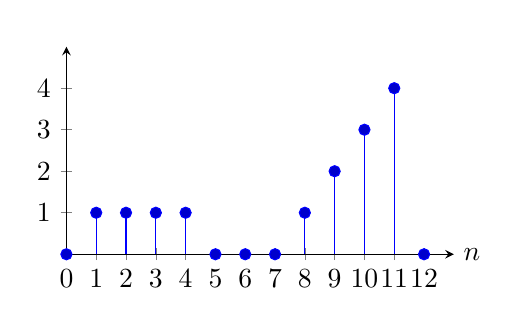
\begin{tikzpicture}
\begin{axis} [width=185pt,height=120pt,
	axis x line=bottom, 
	axis y line=middle, 
	tick align=center,
	every axis x label/.style={at={(current axis.right of origin)},anchor=west},
	every axis y label/.style={at={(current axis.above origin)}, anchor=north east,above=0mm},
	xmin=0, xmax=13,
	xtick={0,...,12},
	xlabel=$n$,
	ymin=0, ymax=5,
	ytick={0,...,4},
	ylabel={$\boldimgworld$}]
\addplot+[ycomb] 
coordinates {(0,0) (1,1) (2,1) (3,1) (4,1) (5,0) (6,0) (7,0) (8,1) (9,2)  (10,3)  (11,4)  (12,0)};
\end{axis}
\end{tikzpicture}
&~
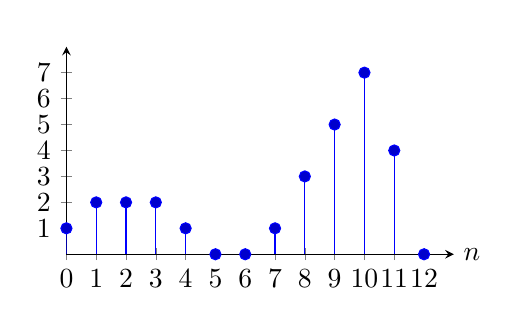
\begin{tikzpicture}
\begin{axis} [width=185pt,height=120pt,
	axis x line=bottom, 
	axis y line=middle, 
	tick align=center,
	every axis x label/.style={at={(current axis.right of origin)},anchor=west},
	every axis y label/.style={at={(current axis.above origin)}, anchor=north east,above=0mm},
	xmin=0, xmax=13,
	xtick={0,...,12},
	xlabel=$n$,
	ymin=0, ymax=8,
	ytick={0,...,7},
	ylabel={$\boldimgsensor$}]
\addplot+[ycomb] 
coordinates {(0,1) (1,2) (2,2) (3,2) (4,1) (5,0) (6,0) (7,1) (8,3) (9,5)  (10,7)  (11,4)  (12,0)};
\end{axis} 
\end{tikzpicture}
\end{array}
$
%\end{center}
}
\caption{Pinhole camera. (left) Input 1D signal, $\boldimgworld$. (right) The output of the two-pixel wide pinhole camera, $\boldimgsensor$.} 
\label{fig:2pixelwidepinhole}
\end{figure}

The output is obtained by multiplying the input vector by the matrix $\mathbf{A}$ shown in \fig{\ref{fig:amats1}}{d}. Each output value is the results of adding up two consecutive input values. The output is nearly identical to the input signal but with a larger magnitude and a bit smoother.

\section{More General Imagers}

Many different optical systems can form cameras and the linear analysis described before can be used to characterize the imaging process.  Even a simple edge will do.  \Fig{\ref{fig:amats3}} shows two non traditional imaging systems that we will analyze in this section. 


\begin{figure}[t]
\centerline{
\includegraphics[width=1\linewidth]{figures/imaging/nontraditional_pinholes_2.eps}
}
\caption{(a) Schematic drawing of an edge camera, and (b) its imaging matrices. (c) A pinspeck camera (an occluder that blocks two of the values on the scene), and (d) its imaging matrices.}
\label{fig:amats3}
\end{figure}

\subsection{Edge Camera}


Consider the example of \fig{\ref{fig:amats3}}{a}. This camera corresponds to an {\bf edge camera}\index{Camera!Edge camera}. This is not a traditional pinhole camera; instead light is blocked only on one side.  




For this camera, the imaging matrix and its inverse are as follows:
%\begin{equation}
%\mathbf{A} = 
%\left( 
%\begin{array}{ccccccccccccc}
%1 & 1 & 1 & 1 & 1 & 1 & 1 & 1 & 1 & 1 & 1 & 1 & 1 \\
%0 & 1 & 1 & 1 & 1 & 1 & 1 & 1 & 1 & 1 & 1 & 1 & 1 \\
%0 & 0 & 1 & 1 & 1 & 1 & 1 & 1 & 1 & 1 & 1 & 1 & 1 \\
%0 & 0 & 0 & 1 & 1 & 1 & 1 & 1 & 1 & 1 & 1 & 1 & 1 \\
%0 & 0 & 0 & 0 & 1 & 1 & 1 & 1 & 1 & 1 & 1 & 1 & 1 \\
%0 & 0 & 0 & 0 & 0 & 1 & 1 & 1 & 1 & 1 & 1 & 1 & 1 \\
%0 & 0 & 0 & 0 & 0 & 0 & 1 & 1 & 1 & 1 & 1 & 1 & 1 \\
%0 & 0 & 0 & 0 & 0 & 0 & 0 & 1 & 1 & 1 & 1 & 1 & 1 \\
%0 & 0 & 0 & 0 & 0 & 0 & 0 & 0 & 1 & 1 & 1 & 1 & 1 \\
%0 & 0 & 0 & 0 & 0 & 0 & 0 & 0 & 0 & 1 & 1 & 1 & 1 \\
%0 & 0 & 0 & 0 & 0 & 0 & 0 & 0 & 0 & 0 & 1 & 1 & 1 \\
%0 & 0 & 0 & 0 & 0 & 0 & 0 & 0 & 0 & 0 & 0 & 1 & 1 \\
%0 & 0 & 0 & 0 & 0 & 0 & 0 & 0 & 0 & 0 & 0 & 0 & 1 
%\end{array}
%\right) .
%\label{eq:edge}
%\end{equation}

\begin{equation}
\mathbf{A} = 
\left[ 
\begin{array}{cccccc}
1 & 1 & 1 & 1 & \dots & 1 \\
0 & 1 & 1 & 1 & ~ & 1 \\
0 & 0 & 1 & 1 & ~ & 1 \\
0 & 0 & 0 & 1 & ~ & 1 \\
\vdots & ~ & ~ & ~ & \ddots & ~ \\
0 & 0 & 0 & 0 & ~ & 1 
\end{array}
\right], 
\mathbf{A}^{-1} = 
\left[ 
\begin{array}{cccccc}
1 & -1 & 0 & 0 & \dots & 0 \\
0 & 1 & -1 & 0 & ~ & 0 \\
0 & 0 & 1 & -1 & ~ & 0 \\
0 & 0 & 0 & 1 & ~ & 0 \\
\vdots & ~ & ~ & ~ & \ddots & ~  \\
0 & 0 & 0 & 0 & ~ & 1 
\end{array}
\right]
\label{eq:edge}
\end{equation}

If we consider the same input as in the pinhole camera example in the previous section, the output signal for the corner camera will look like (\fig{\ref{fig:1dcornercamera}}):

\begin{figure}[h]
\centerline{
%\begin{center}
$
\begin{array}{cc}
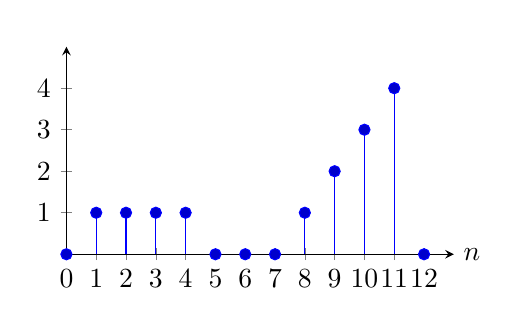
\begin{tikzpicture}
\begin{axis} [width=185pt,height=120pt,
	axis x line=bottom, 
	axis y line=middle, 
	tick align=center,
	every axis x label/.style={at={(current axis.right of origin)},anchor=west},
	every axis y label/.style={at={(current axis.above origin)}, anchor=north east,above=0mm},
	xmin=0, xmax=13,
	xtick={0,...,12},
	xlabel=$n$,
	ymin=0, ymax=5,
	ytick={0,...,4},
	ylabel={$\boldimgworld$}]
\addplot+[ycomb] 
coordinates {(0,0) (1,1) (2,1) (3,1) (4,1) (5,0) (6,0) (7,0) (8,1) (9,2)  (10,3)  (11,4)  (12,0)};
\end{axis}
\end{tikzpicture}
&~
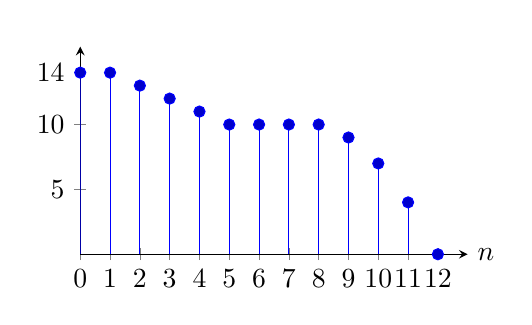
\begin{tikzpicture}
\begin{axis} [width=185pt,height=120pt,
	axis x line=bottom, 
	axis y line=middle, 
	tick align=center,
	every axis x label/.style={at={(current axis.right of origin)},anchor=west},
	every axis y label/.style={at={(current axis.above origin)}, anchor=north east,above=0mm},
	xmin=0, xmax=13,
	xtick={0,...,12},
	xlabel=$n$,
	ymin=0, ymax=16,
	ytick={0,5,10,14},
	ylabel={$\boldimgsensor$}]
\addplot+[ycomb] 
coordinates {(0,14) (1,14) (2,13) (3,12) (4,11) (5,10) (6,10) (7,10) (8,10) (9,9)  (10,7)  (11,4)  (12,0)};
\end{axis} 
\end{tikzpicture}
\end{array}
$
%\end{center}
}
\caption{Edge camera. (left) Input 1D signal, $\boldimgworld$. (right) The output of an edge camera, $\boldimgsensor$.} 
\label{fig:1dcornercamera}
\end{figure}

The output now looks very different than that of a pinhole camera. In the pinhole camera, the output is very similar to the input. This is not the case here where the output looks like the integral of the input (reversed along the horizontal axis). Note that the first value of $\boldimgsensor$ is equal to the sum of all the values of $\boldimgworld$:
\begin{equation}
\imgsensor \left[0 \right] = \sum_{n=0}^{12} \imgworld \left[n \right]
\end{equation}

\Fig{\ref{fig:amats3}}{b} illustrates the imaging matrix, $\mathbf{A}$, and reconstruction matrices for the imager of \eqn{\ref{eq:edge}}. You can think of this imager as computing an integral of the input signal. Therefore, its inverse looks like a derivative. The regularized inverse looks like a blurred derivative (we will talk more about blurred derivatives in \chap{\ref{chapter:image_derivatives}}).
%, as well as for an edge imager where the responses are blurred across several sensor elements.


\subsection{Pinspeck Camera}

\Fig{\ref{fig:amats3}}{c} shows another nontraditional imager. Now, instead of a pinhole we have an occluder. The occluder blocks part of the light (complementary to the large-hole pinhole camera shown in \fig{\ref{fig:amats1}}{c}). What the camera sensor records is the shadow of the occluder.
\marginnote{The shadow of an object is related to the negative of a picture taken of the environment around the object.}
We can write the imaging matrix $\mathbf{A}$, which corresponds to 1-$\mathbf{A}_{pinhole}$ as shown in \fig{\ref{fig:amats1}}{d}. \Fig{\ref{fig:amats3}}{d} also shows its inverse and the regularized inverse. This camera is called a {\bf pinspeck camera}\index{Camera!Pinspeck camera} \cite{CohenPinspeck,Torralba2014} and has also been used in practice. 

In the example of \fig{\ref{fig:amats3}}{c}, the occluder has the size of the wide pinhole from  \fig{\ref{fig:amats1}}{c}. The following plots shows, \fig{\ref{fig:pinspeck_output_plot}}{left}, the input scene (same as in the previous examples) and, \fig{\ref{fig:pinspeck_output_plot}}{right}, the output recorded by the camera sensor of the pinspeck camera. 
\begin{figure}
\centerline{
%\begin{center}
$
\begin{array}{cc}
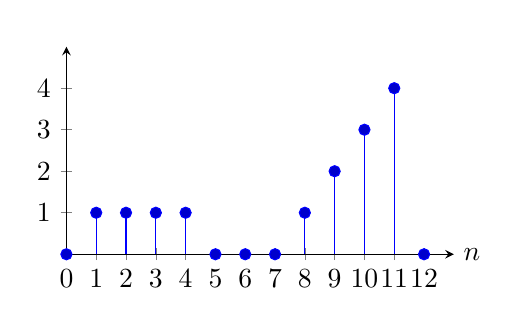
\begin{tikzpicture}
\begin{axis} [width=185pt,height=120pt,
	axis x line=bottom, 
	axis y line=middle, 
	tick align=center,
	every axis x label/.style={at={(current axis.right of origin)},anchor=west},
	every axis y label/.style={at={(current axis.above origin)}, anchor=north east,above=0mm},
	xmin=0, xmax=13,
	xtick={0,...,12},
	xlabel=$n$,
	ymin=0, ymax=5,
	ytick={0,...,4},
	ylabel={$\boldimgworld$}]
\addplot+[ycomb] 
coordinates {(0,0) (1,1) (2,1) (3,1) (4,1) (5,0) (6,0) (7,0) (8,1) (9,2)  (10,3)  (11,4)  (12,0)};
\end{axis}
\end{tikzpicture}
&~
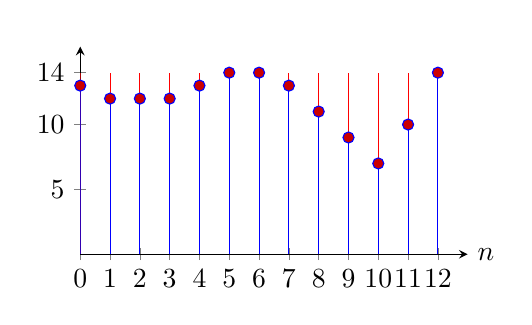
\begin{tikzpicture}
\begin{axis} [width=185pt,height=120pt,
	axis x line=bottom, 
	axis y line=middle, 
	tick align=center,
	every axis x label/.style={at={(current axis.right of origin)},anchor=west},
	every axis y label/.style={at={(current axis.above origin)}, anchor=north east,above=0mm},
	xmin=0, xmax=13,
	xtick={0,...,12},
	xlabel=$n$,
	ymin=0, ymax=16,
	ytick={0,5,10,14},
	ylabel={$\boldimgsensor$}]
\addplot[ycomb,red] 
coordinates {(0,14) (1,14) (2,14) (3,14) (4,14) (5,14) (6,14) (7,14) (8,14) (9,14)  (10,14)  (11,14)  (12,14)};
\addplot+[ycomb,blue,fill=blue,mark=*] 
coordinates {(0,13) (1,12) (2,12) (3,12) (4,13) (5,14) (6,14) (7,13) (8,11) (9,9)  (10,7)  (11,10)  (12,14)};
\end{axis} 
\end{tikzpicture}
\end{array}
$
%\end{center}
}
\caption{Pinspeck camera. (left) Input 1D signal, $\boldimgworld$. (right) The output of a pinspeck camera, $\boldimgsensor$.} 
\label{fig:pinspeck_output_plot}
\end{figure}

The output is now a signal with a wide dynamic range (a max value of 14, which correspond to the sum of the values in $\boldimgworld$) and with fluctuations due to the shadow of the occluder on the camera sensor. If there was no occluder, then the output would be a constant signal of value 14. In red we show the effect of the shadow, which is the light missing because of the presence of the occluder. You can see how the missing signal is identical to the output of the two-pixel wide pinhole camera but reversed in sign.


%\begin{figure}
%\centerline{
%\sublabel{a}{\includegraphics[width=0.45\linewidth]{figures/imaging/ph3.pdf}}}
%\centerline{
%\sublabel{b}{\includegraphics[width=0.45\linewidth]{figures/imaging/amat31.pdf}}
%\sublabel{c}{\includegraphics[width=0.45\linewidth]{figures/imaging/amat34.pdf}}
%}
%\caption{
%(a) An edge camera (b) Visualization of idealized imaging matrices:  The imaging matrix relating scene intensities to sensor readings; the inverse of that matrix;  the regularized inverse.  (c) A blurred edge imaging matrix, and its inverse and regularized inverse }
%\label{fig:amats3}
%\end{figure}





\subsection{Corner Camera}  

To show a real-world example of a more general imager, let us consider the {\bf corner camera}\index{Camera!Corner camera} \cite{Bouman17}.  This is similar to the edge
camera of \eqn{\ref{eq:edge}} and \fig{\ref{fig:amats3}}, but with
slightly more complicated geometry.  As shown in
\fig{\ref{fig:ccmodel}}{a}, a vertical edge partially blocks a scene from view, creating intensity variations on the ground, observable by viewing those intensity variations from around the corner.


\begin{figure}[t]
\centerline{
\sublabel{a}
{\includegraphics[width=0.4\linewidth]{figures/imaging/cornercam.pdf}}
\sublabel{b}
{\includegraphics[width=0.4\linewidth]{figures/imaging/cornerKey.pdf}}}
\caption{The corner camera \cite{Bouman17}.  (a) Objects, such as the cylinders labeled A and B, hidden behind a corner from a camera nonetheless cause a very small intensity differences in the ambient illumination falling on the ground.
%, observable from the camera as a very small change in the light intensity reflecting from the ground.  The image reconstruction operation is analogous to that for the edge camera of \fig{\ref{fig:amats3}}:  we subtract the reflected intensities observed at one orientation angle, say $\theta_A$ from those observed at another, say $\theta_B$. 
(b) the spatial mask is multiplied by the observed reflected ground image.}
\label{fig:ccmodel}
\end{figure}


In practice, we will subtract a mean image from our observations of the ground plane, so in the rendering equation below, we will only consider components of
the scene that may change over time, under the assumption that what we want to image behind the corner (e.g., a person) is moving.  We will call these intensities
$S(\phi, \theta)$ ($S$ for the subject), where $\phi$ measures
vertical inclination and $\theta$ measures azimuthal angle, relative to position where the vertical edge intersects the ground plane.  Integrating the light intensities falling on the ground plane, the
observed intensities on the ground will be $\boldimgground (r, \theta)$, where the
polar coordinates $r$ and $\theta$ are measured with respect to the corner.
Assuming Lambertian diffuse reflection from the ground plane, we have, for the observed intensities $\boldimgground (r, \theta)$,
\begin{equation}
 \boldimgground (r, \theta) = \int_{\phi=0}^{\phi=\pi} \int_{\xi=0}^{\xi=\theta}
 \cos(\phi) S(\phi, \xi) \mbox{d} \phi \mbox{d} \xi,
\label{eq:corner}
\end{equation}
where the $\cos(\phi)$ term in \eqn{\ref{eq:corner}} follows from the equation for surface reflection, \eqn{\ref{eq:lambert}}.



The dependence of the observation, $\boldimgground$, on vertical variations in
$S(\phi, \theta)$ is very weak, just through the $\cos(\phi)$ term.
We can integrate over $\phi$ first, to form the 1D signal,
$\imgworld (\xi)$:
\begin{equation}
  \imgworld (\xi) = \int_{\phi=0}^{\phi=\pi} 
  \cos(\phi) S(\phi, \xi) \mbox{d} \phi 
\label{eq:xcorner}
\end{equation}

Then, to a good approximation, \eqn{\ref{eq:corner}} has the form,
\begin{equation}
 \boldimgground (r, \theta) \approx \int_{\xi=0}^{\xi=\theta}
 \imgworld (\xi) \mbox{d} \xi,
\label{eq:corner1d}
\end{equation}
where $\imgworld (\xi)$ is a 1D image of the scene around the corner from the vertical edge.

\Fig{\ref{fig:ccmodel}} shows the corner camera geometry for a three-dimensional (3D) scene.  \Fig{\ref{fig:ccmodel}}{a} shows two objects, such as the cylinders labeled A and B, hidden behind a corner from a camera. Despite being behind the corner they cause a very small intensity differences in the ambient illumination falling on the ground, observable from the camera as a very small change in the light intensity reflecting from the ground. Can we reconstruct the scene hidden behind the corner using just the intensities observed on the ground? The image reconstruction operation is analogous to that for the edge camera of \fig{\ref{fig:amats3}}:  we subtract the reflected intensities observed at one orientation angle, say $\theta_A$ from those observed at another, say $\theta_B$. 

If we sample \eqn{\ref{eq:corner1d}} in its continuous variables, we
can write it in the form $\boldimgground = \mathbf{A} \boldimgworld$.  Solving \eqn{\ref{eq:deriv2}}
for the multiplier to apply to $\boldimgground$ to estimate $\boldimgworld$ yields the form shown in
\fig{\ref{fig:ccmodel}}{b}.  \Fig{\ref{fig:ccmodel}}{b} shows the spatial mask to be multiplied by the observed reflected ground image, with the result summed over all spatial pixels in order to estimate the light coming from around the corner at one particular orientation angle relative to the corner, in this case approximately 45 degrees. We see that the way to read the 1D signal from the ground plane is to take a derivative with respect to angle.  This makes intuitive sense, as the light intensities on the ground integrate all the light up to the angle of the vertical edge.  To find the 1D signal at the angle of the edge, we ask, ``What does one pie-shaped ray from the wall see that the pie-shaped ray next to it doesn't see?''


It can be shown \cite{Bouman17} that the image intensities from around-the-corner scenes introduce a perturbation of about $\frac{1}{1,000}$ to the light reflected from the ground from all sources.   
By averaging image intensities over the appropriate pie-shaped regions on the ground at the corner (\fig{\ref{fig:ccmodel}}[b]), one can extract a 1D image as a function of time from the scene around the corner.  \Fig{\ref{fig:cctraces}} shows two 1D videos reconstructed from one (\fig{\ref{fig:cctraces}}[a]) and two (\fig{\ref{fig:cctraces}}[b]) people walking around the corner.  By processing videos of very faint intensity changes on the ground, we can infer a 1D video of the scene around the corner.  The image inversion formulas were derived using inversion methods very similar to \eqn{\ref{eq:deriv2}}.  The corner camera is just one of the many possible instantiations of a computational imaging system.


\begin{figure}[t]
\centerline{
\includegraphics[width=0.9\linewidth]{figures/imaging/corner_camera_3D.eps}
}
%\centerline{
%\sublabel{a}
%{\includegraphics[width=0.4\linewidth]{figures/imaging/corner.jpg}}
%\sublabel{b}
%{\includegraphics[width=0.4\linewidth]{figures/imaging/2people.jpg}}}
%\centerline{
%\sublabel{c}
%{\includegraphics[width=0.2\linewidth]{figures/imaging/cctrace.pdf}}
%\sublabel{d}
%{\includegraphics[width=0.2\linewidth]{figures/imaging/cctrace2.pdf}}
%}
\caption{Outdoor corner camera \cite{Bouman17} experiments. (a) Camera recording ground plane intensities.  (b) Two people walking around the corner, hidden from direct view of the camera. (c) Corner camera trace with one person moving. (d) Corner camera trace with two people moving.  Angle from the corner is plotted vertically, and time is plotted horizontally.}
\label{fig:cctraces}
\end{figure}

\marginnote{People moving out of view around a corner cause small, invisible changes in the light reflecting from the ground. These faint changes occur at nearly every corner and can be used to read-out 1D images of the people around the corner.}[0in]


%% 
%% \subsection{Pinhole lightfield imager}
%% An array of pinholes.  How to construct and photograph that?
%% 


\section{Concluding Remarks}  
Treating cameras as general linear systems allows for the machinery of linear algebra to be applied to camera design and processing.  We reviewed several simple camera systems, including cameras utilizing pinholes, pinspecks, and edges to form images.
 % Bill
% \chapter{Representing Images and Geometry}
\label{chapter:geometry_homogeneous}

%\chapter{Imaging Geometry}

%\reviewcomment{Chapter partially completed. References missing. Several figures missing. Side notes missing.}

%\reviewcomment{Question: this chapter could go much later, should it go inside  visual understanding part? That is closer to the applications when this material will become useful.}

%For many computer vision tasks, we need to know the relationship between the positions of points in the world and where they appear in the image taken by a camera.  Determining those relationships, which involves both measuring properties of a camera and also its position and orientation, is called {\em camera calibration}. To perform the calculations needed for camera calibration it is convenient to use a set of coordinates known as homogeneous coordinates.

%In this chapter we will introduce the formulation that is commonly used when studying scene geometry.

\section{Introduction}


Before we dive into the material of this chapter, let's start by questioning the way in which we have been representing images up to now. In most of the chapters, we have represented images as ordered arrays of pixel values, each pixel described by its grayscale value (or three arrays for color images). We will call this representation the {\bf ordered array}.
\begin{equation}
\boldimg = 
\left[
\begin{matrix}
\img [1,1] & \dots & \\
\vdots & \img [n,m] & \vdots \\
 & \dots  & \img [N,M] \\
\end{matrix}
\right]
%\left[x [n,m] \right]
\end{equation}
Each value is a sample on a regular spatial grid. In this notation $s$ represents the pixel intensity at one location. This is the representation we are most used to and the typical representation used when taking a signal processing perspective. It makes it simpler to describe operations such as convolution.

However, an image can be represented in different ways, making explicit certain aspects of the information present on the input. What else could we do to represent an image? Another very different, but equivalent, representation is to encode an image as a collection of points, indicating its color and location explicitly. In this case, an image is represented as a {\bf set of pixels}:
\begin{equation}
\left\{ [\img_i,x_i,y_i] : i \right\}
\label{eq:set_of_pixels}
\end{equation}
 where $\img_i$ is the pixel intensity (or color) recorded at location $(x_i,y_i)$. 
 This representation makes the geometry explicit. It might seem like a trivial representation but it makes some operations easy (and others complex). For instance, we can apply geometric transformations easily by directly working with the spatial coordinates. Imagine you want to translate an image, described by \eqn{\ref{eq:set_of_pixels}}, to the right by one pixel, you can do that easily by simply creating the new image defined by the set of translated pixels: $\left\{ [\img_i,x_i+1,y_i] : i \right\}$. 

 \marginnote{Representing images as sets of points is very common in geometry-based computer vision. We will use this representation extensively in the following chapters.}
 
 Although both previous representations might seem equivalent, the set representation makes it easy to deal with other image geometries where the points are not on a regular array. 
 
 That representation can also be extended by representing geometry in different ways such as using homogeneous coordinates, or positional encoding. We will discuss homogeneous coordinates in this chapter. 

The previous two representations are not the only ways in which we can represent images. Another option is to represent an image as a continuous function whose input is
a location $(x, y)$ and it output is an intensity, or a color, $\img$:
\begin{equation}
   \img (x,y) = f_{\theta}(x,y)
\end{equation}
This image representation is commonly used when we want to make image priors more explicit. The function $f_{\theta}$ is parameterized by the coefficients $\theta$. This function becomes especially interesting when the parameters $\theta$ are different than the original pixel values. They will have to be estimated from the original image. But once learned, the function $f$ should be able to take as input continuous spatial variables.

These three representations induce different ways of thinking about architectures to process the visual input. These representations are not opposed and can be used simultaneously.

The ordered array of pixels is the format that computers take as input when visualizing images. However, a set of pixels is the most common format when thinking about three-dimensional (3D) geometry and image formation. Therefore, it is always important to be familiar with how to transform any representation into an ordered array.

%Let's start by studying some two-dimensional (2D) geometric image transformations and we will use them as a excuse to introduce homogeneous coordinates. %Homogeneous coordinates will become very important when talking about 3D geometry and 2D image formation. 

We will start by introducing homogeneous coordinates, an important tool that will simplify the formulation of perspective projection. 


\section{Homogeneous and Heteregenous Coordinates}


Homogeneous coordinates represent a vector of length $N$ by a vector of length $N+1$.
The transformation rule from heterogeneous to homogeneous coordinates is simply to add an additional coordinate, 1, to the heterogeneous coordinates as shown here:
\begin{equation}
    \begin{pmatrix}
    x \\
    y 
    \end{pmatrix}
    \rightarrow 
    \begin{bmatrix}
    x \\
    y \\
    1
    \end{bmatrix}
    \label{eq:2dhomo}
\end{equation}
It is the same if the vector has three dimensions:
\begin{equation}
    \begin{pmatrix}
    x \\
    y \\
    z
    \end{pmatrix}
    \rightarrow 
    \begin{bmatrix}
    x \\
    y \\
    z \\
    1
    \end{bmatrix}
    \label{eq:3dhomo}
\end{equation}


We will refer to conventional Cartesian coordinate descriptions of a point in 2D, such as $(x,y)$, or 3D, such as $(x,y,z)$, as {\bf heterogeneous coordinates} and write with rounded brackets in this chapter.  We denote their corresponding {\bf homogeneous coordinate} representations by square bracketed vectors.

\marginnote{August Ferdinand Möbius, a German mathematician and astronomer, introduced homogeneous coordinates in 1827. He also cocreated the famous Möbius strip.}

The homogeneous coordinates have the additional rule that all (non-zero) scalings of a homogeneous coordinate vector are equivalent.  For example, to represent a 2D point, we have (transforming from heterogeneous to homogeneous coordinates),
\begin{equation}
    %(x,y) \rightarrow 
    \begin{bmatrix}
    x \\
    y \\
    1
    \end{bmatrix}
    \equiv 
    \begin{bmatrix}
    \lambda x \\
    \lambda y \\
    \lambda
    \end{bmatrix}
\end{equation}
for any non-zero scalar, $\lambda$. To go from homogeneous coordinates back to the heterogeneous representation of the point, we divide all the entries of the homogeneous coordinate vector by their last dimension:

\begin{equation}
    \begin{bmatrix}
    x \\
    y \\
    w
    \end{bmatrix}
    \rightarrow 
    \begin{pmatrix}
    x/w \\
    y/w 
    \end{pmatrix}
\end{equation}

\Fig{\ref{fig:homogeneousAndHeteregeneous}} illustrates how homogeneous and heterogeneous coordinates relate to each other geometrically. A point in homogeneous coordinates is scale invariant (any point within the line that passes through the origin translates into the same point in heterogeneous coordinates). We can already see that this is closely related to the operation performed by perspective projection. 

\begin{figure}
\centerline{
\includegraphics[width=0.7\linewidth]{figures/imaging_geometry/homogeneousAndHeteregeneous_VS3.eps}
}
\caption{Transformation rule between heterogeneous and homogeneous coordinates in 2D. All the points along the dotted line correspond to the same point in heterogeneous coordinates. Note that the points $(x,y)$ and $(x,y,1)$ live in different spaces.}
\label{fig:homogeneousAndHeteregeneous}
\end{figure}

It is important to mention that while you can add two points in heterogeneous coordinates, you can not do the same in homogeneous coordinates!

\marginnote{Using homogeneous coordinates, we can place a point at infinity by setting $w=0$. This is called the {\bf ideal point}.}\index{Ideal point}

\section{2D Image Transformations}
\label{sect:2dtransforms}

One important operation in computer vision (and in computer graphics) is geometric transformations of shapes. Some of the common transformations we'll want to represent include  translation, rotation, scaling, and shearing (see \fig{\ref{fig:2dtransformations_clock}}). These transformations can be written as affine transformations of the coordinate system. The mathematical description of these transformations becomes surprisingly simple when using homogeneous coordinates, and they will become the basis for more complex operations such as 3D perspective projection and camera calibration as we will see in later sections.


\begin{figure}
\centerline{
\includegraphics[width=1\linewidth]{figures/imaging_geometry/2d_transformations.eps}
}
\caption{2D geometric transformations. 
%On the left we see the original image. The next four transformations correspond to translation, rotation, scaling and shear. Those four transformations can be easily described with matrices. 
The final transformation is an arbitrary warping with a more complex deformation field.}
\label{fig:2dtransformations_clock}
\end{figure}

%\subsection{Translation, Rotation, Scaling and Shear.}

We'll explore the use of homogeneous coordinates for describing 2D geometric transformations first, then see how they can easily represent 3D perspective projection.


\subsection{Translation}

Consider a translation by a 2D vector, $(t_x, t_y)$ as shown in \fig{\ref{fig:translations}}. We'll denote the coordinates after the transformation with a prime. In heterogeneous coordinates, we have
\begin{equation}
    \begin{pmatrix}
    x' \\
    y' 
    \end{pmatrix}
    =
    \begin{pmatrix}
    x \\
    y 
    \end{pmatrix}
    +
    \begin{pmatrix}
    t_x \\
    t_y 
    \end{pmatrix}
\end{equation}
We can write this translation in homogeneous coordinates by the product:
\begin{equation}
    \begin{bmatrix}
    x' \\
    y' \\
    1
    \end{bmatrix}
    =
    \begin{bmatrix}
    1 & 0 & t_x \\
    0 & 1 & t_y \\
    0 & 0 & 1
    \end{bmatrix}
    \begin{bmatrix}
    x \\
    y \\
    1
    \end{bmatrix}
\end{equation}
What is interesting is that we have transformed an addition into a product by a matrix, $\mathbf{T}$, and a vector, $\mathbf{p}$, in homogeneous coordinates. 
Rewriting the equation above as:
\begin{equation}
    \mathbf{p}' = \mathbf{T} \mathbf{p},
\end{equation}
with the homogeneous matrix, $\mathbf{T}$, defined as
\begin{equation}
    \mathbf{T} =             
    \begin{bmatrix}
    1 & 0 & t_x \\
    0 & 1 & t_y \\
    0 & 0 & 1
    \end{bmatrix}
\end{equation}
For calculations in homogeneous coordinates, both matrices and vectors are only defined up to an arbitrary (non-zero) multiplicative scaling factor.

To cascade two translation operations $\mathbf{t}$ and  $\mathbf{s} $, in heterogeneous coordinates, we have 
\begin{equation}
     \mathbf{p}' = \mathbf{p} + \mathbf{t}  + \mathbf{s}   
\end{equation}


\begin{figure}[ht]
\centerline{
\includegraphics[width=.7\linewidth]{figures/imaging_geometry/translations.eps}
}
\caption{(left) Translation. (right) Composition of two consecutive translations.}
\label{fig:translations}
\end{figure}


In homogeneous coordinates, we cascade the corresponding translation matrices:
\begin{equation}
     \mathbf{p}' = \mathbf{S} \mathbf{T} \mathbf{p},
\end{equation}
where the homogeneous translation matrix, $\mathbf{S}$, corresponding to the offset $\mathbf{s}$, is:
\begin{equation}
    \mathbf{S} =            
    \begin{bmatrix}
    1 & 0 & s_x \\
    0 & 1 & s_y \\
    0 & 0 & 1
    \end{bmatrix}
\end{equation}

You can check that:
\begin{equation}
    \begin{bmatrix}
    1 & 0 & t_x \\
    0 & 1 & t_y \\
    0 & 0 & 1
    \end{bmatrix}
    \begin{bmatrix}
    1 & 0 & s_x \\
    0 & 1 & s_y \\
    0 & 0 & 1
    \end{bmatrix}
    =
    \begin{bmatrix}
    1 & 0 & t_x+s_x \\
    0 & 1 & t_y+s_y \\
    0 & 0 & 1
    \end{bmatrix}
\end{equation}

In summary, in homogeneous coordinates a translation becomes a product with a matrix, and chaining translations can be done by multiplying the matrices together. The benefits of using the homogeneous coordinates will become more obvious later.

\subsection{Scaling}

Scaling the $x$-axis by $s_x$ and the $y$-axis by $s_y$, shown in \fig{\ref{fig:scaling}}, yields the transformation matrix in homogeneous coordinates,
\begin{equation}
    \mathbf{S} =             
    \begin{bmatrix}
    s_x & 0 & 0 \\
    0 & s_y & 0 \\
    0 & 0 & 1
    \end{bmatrix}
\end{equation}

The scaling matrix is a diagonal matrix. 

\begin{figure}[ht]
\centerline{
\includegraphics[width=.6\linewidth]{figures/imaging_geometry/scaling.eps}
}
\caption{Non-uniform or anisotropic scaling. In this example the $y$-axis is compressed and the $x$-axis is expanded.}
\label{fig:scaling}
\end{figure}

Uniform scaling is obtained when $s_x=s_y$, otherwise the scaling is nonuniform or anisotropic. After uniform scaling, all of the angles are preserved. In all cases, parallel lines remain parallel. Areas are scaled by the determinant of the scaling matrix.


\subsection{Rotation}

For a rotation by an angle $\theta$, \fig{\ref{fig:rotation}}, we simply have the matrix in homogeneous coordinates:
\begin{equation}
    \mathbf{R} =             
    \begin{bmatrix}
    \cos(\theta) & \sin(\theta) & 0 \\
    -\sin(\theta) & \cos(\theta) & 0 \\
    0 & 0 & 1
    \end{bmatrix}
\end{equation}


\begin{figure}
\centerline{
\includegraphics[width=.6\linewidth]{figures/imaging_geometry/rotation.eps}
}
\caption{Rotation by an angle $\theta$ counterclockwise around the origin.}
\label{fig:rotation}
\end{figure}


As in the case of the translation, a rotation in homogeneous coordinates is a product
\begin{equation}
    \mathbf{p}' = \mathbf{R} \mathbf{p},
\end{equation}
Also, as we should expect, chaining two rotations with angles $\alpha$ and $\beta$, is the same than applying a rotation with an angle $\alpha+\beta$. You can check that multiplying the two rotation matrices you get the right transformation. 

The determinant of a rotation matrix is 1 and the matrix is orthogonal, that is the transpose is equal to the inverse: $\mathbf{R}^\transpose = \mathbf{R}^{-1}$. The inverse is also a rotation matrix. The distance between any point and the origin does not change after a rotation. 

In heterogeneous coordinates, the transformation can also be written in the same way but using only the upper-left $2\times2$ matrix. Representing rotations in homogeneous coordinates has no benefit with respect to heterogeneous coordinates. But the advantage is that now both rotation and translation are written in the same way! They are both products of a matrix times a vector, so that they can be combined as we will discuss in \sect{\ref{sec:chaining_transformations}}.   


If the angle of rotation is very small, then we can approximate the rotation matrix by its Taylor development
(for small $x$, $\sin(x) \approx x$ and $\cos(x) \approx 1$):
\begin{equation}
    \mathbf{R} \simeq            
    \begin{bmatrix}
    1 & \theta & 0 \\
    -\theta & 1 & 0 \\
    0 & 0 & 1
    \end{bmatrix}
\end{equation}

For small angles a rotation becomes a shear, which we will discuss next. In general, for all angles, a rotation can be written as two shears and a scaling.

Rotations in 3D become more complex as there are multiple possible parametrizations. 


\subsection{Shearing}

Shearing involves scale factors in the off-diagonal matrix locations, as shown in the matrix, $\mathbf{Q}$:
\begin{equation}
    \mathbf{Q} =             
    \begin{bmatrix}
    1 & q_x & 0 \\
    q_y & 1 & 0 \\
    0 & 0 & 1
    \end{bmatrix}
\end{equation}

\Fig{\ref{fig:shear}} shows examples with an horizontal shear ($qx=1, q_y=0$), a vertical shear ($q_x=0, q_y=1$), and an arbitrary shear. 

\begin{figure}
\centerline{
\includegraphics[width=1\linewidth]{figures/imaging_geometry/shear.eps}
}
\caption{Three examples of shear transformation.}
\label{fig:shear}
\end{figure}

In the example of the horizontal shear, the points are displaced along horizontal lines by displacement proportional to the $y$ coordinate, $x'=x+q_y y$. 

In a shear, lines are mapped to lines, parallel lines remain parallel, (non-zero) angles between lines change.

\subsection{Chaining Transformations}
\label{sec:chaining_transformations}

As we have seen, homogeneous coordinates allows using all the four different transformations as matrix multiplications. We can now build complex transformations by combining these four transformations:
\begin{equation}
    \mathbf{p}' = 
    \begin{bmatrix}
    1 & q_x & 0 \\
    q_y & 1 & 0 \\
    0 & 0 & 1
    \end{bmatrix}
    \begin{bmatrix}
    s_x & 0 & 0 \\
    0 & s_y & 0 \\
    0 & 0 & 1
    \end{bmatrix}
    \begin{bmatrix}
    \cos(\theta) & \sin(\theta) & 0 \\
    -\sin(\theta) & \cos(\theta) & 0 \\
    0 & 0 & 1
    \end{bmatrix}
    \begin{bmatrix}
    1 & 0 & t_x \\
    0 & 1 & t_y \\
    0 & 0 & 1
    \end{bmatrix}
    \mathbf{p}
\end{equation}

%\begin{equation}
%    \mathbf{p}' = 
%    \mathbf{M}  
%    \mathbf{p}
%\end{equation}

 In heterogeneous coordinates the translation will have to be modeled as an addition breaking the homogeneity of this equation. The transformations described in this section are summarized in \fig{\ref{fig:2dtransformations}}.

\begin{figure}
\centerline{
\includegraphics[width=1\linewidth]{figures/imaging_geometry/2d_transforms.eps}
}
\caption{Summary of 2D geometric transformations and their formulation in homogeneous coordinates.}
\label{fig:2dtransformations}
\end{figure}


As matrix operation are noncommutative, the order in which operations are done is important (i.e., it is not the same to rotate with respect to the origin and then translate, as it is to translate and then rotate). All of the geometric transformations we have described are relative to the origin. If you want to rotate an image around an arbitrary central location, then you need to first translate to put that location at the origin, then rotate and then translate back. 

\begin{equation}
    \mathbf{p}' = 
    \begin{bmatrix}
    1 & 0 & t_x \\
    0 & 1 & t_y \\
    0 & 0 & 1
    \end{bmatrix}
    \begin{bmatrix}
    \cos(\theta) & \sin(\theta) & 0 \\
    -\sin(\theta) & \cos(\theta) & 0 \\
    0 & 0 & 1
    \end{bmatrix}
    \begin{bmatrix}
    1 & 0 & -t_x \\
    0 & 1 & -t_y \\
    0 & 0 & 1
    \end{bmatrix}
    \mathbf{p}
\end{equation}

Chaining transformations in such a way is a very important tool in computer graphics and we will also use it extensively as we dive deeper into geometry. 

When chaining rotations and translations only we will have a {\bf euclidean transformation} 
\index{Euclidean transformation}
(lengths and angles between lines are preserved). A {\bf similarity transform}
\index{Similarity transform}
is the result of chaining a rotation, translation and scaling (with uniform scaling, $s_x=s_y$). In this case angles are preserved but not lengths. Chaining all transformations results in an {\bf affine transformation}. 
\index{Affine transformation}
Each set of transformations forms a group.  

\subsection{Generic 2D Transformations}

In general, chaining translations, scalings, rotations and shears will result in a generic matrix with the form:
\begin{equation}
    \mathbf{p}' = 
    \begin{bmatrix}
    a & b & c \\
    d & e & f \\
    0 & 0 & 1
    \end{bmatrix}
    \mathbf{p}
\end{equation}
Any transformation with that form (6 degrees of freedom) is an affine transformation. An affine transformation has the property that parallel lines will remain parallel after the transformation; however, lengths and non-zero angles might change. 

As the last row of the transformation is $[0,0,1]$, one could be tempted to drop it and go directly from homogeneous to heterogeneous, using the top $2 \times 3$ matrix, but this will only work if the input vector has a 1 in the third component. 

What happens if we have 9 degrees of freedom?

\begin{equation}
    \mathbf{p}' = 
    \begin{bmatrix}
    a & b & c \\
    d & e & f \\
    g & h & i
    \end{bmatrix}
    \mathbf{p}
\end{equation}
In fact we only have 8 degrees of freedom as a global scaling of the matrix does not change the homogeneous coordinates. The set of transformations described by this full matrix becomes more general than the transformations described in the previous sections. The additional degrees of freedom include {\bf elations} and {\bf projective transformations}. 
\index{Projective transformation}

\subsection{Geometric Transformations as Convolutions}

In \chap{\ref{chapter:linear_image_filtering}} we showed how certain geometric transformations can be written as convolutions (such as the translation) while others cannot (such as rotations, scalings, shears, etc.). However, things change when adding geometry explicitly to the image representation! 

Once geometry is added to the representation, all of the transformations we discussed before can be implemented as one-dimensional (1D) convolutions over the locations as shown in the diagram in \fig{\ref{fig:rotation_as_convolution}}. 


\begin{figure}[ht]
\centerline{
\includegraphics[width=.6\linewidth]{figures/imaging_geometry/rotation_as_convolution.eps}
}
\caption{Geometric transformation as a convolution. The input and output signals are represented as pixel sets with explicit geometry. The convolution kernels are $w_x$ and $w_y$, corresponding to one dimensional convolutions as they only mix input features within the same input vector. The output intensity values are the same as the input.}
\label{fig:rotation_as_convolution}
\end{figure}

In the diagram (\fig{\ref{fig:rotation_as_convolution}}), each input element is a vector
$(x_i,y_i,\img_i)$
where $x_i$, $y_i$ are the pixel location, and $\img_i$ is the pixel intensity at that location. 
The convolution kernels are: $w_x=[\cos ( \theta), \sin ( \theta)]$ and  $w_y=[-\sin ( \theta), \cos ( \theta)]$. The weights are the same for all inputs. The output is also represented using position explicitly: $(x'_i,y'_i,\img'_i)$.


However, note that to perform a convolution on the output intensity will require translating the position encoding back into an image on a rectangular grid. For instance, after a rotation, the locations for the intensity values will change and the pixels will not lie on a rectangular grid anymore. The convolution kernels for the intensity channel will have to be transformed too.

\section{Lines and Planes in Homogeneous Coordinates}

One interesting application of homogeneous coordinates is to use it to describe lines and planes and perform operations with them. In 2D, the equation of a line is $ax+by+c=0$, which can be written in homogeneous coordinates as
\begin{equation}
    ax+by+c=0 \rightarrow 
    \begin{bmatrix}
    a & b & c 
    \end{bmatrix}
    \begin{bmatrix}
    x \\
    y \\
    1
    \end{bmatrix}
    = 0
\end{equation}

In homogeneous coordinates, the equation of a line is the dot product:
\begin{equation}
    \boldsymbol{l} ^\transpose \mathbf{p} = 0
\end{equation}
where $\boldsymbol{l}^\transpose = \left [a, b, c\right ]$. Therefore, a point $\mathbf{p}$, belongs to the line when $\boldsymbol{l}$ and $\mathbf{p}$ are perpendicular. 


This representation of the line is in homogeneous coordinates because it is scale invariant. This is, $\left [a, b, c\right ]$ is the same line as $\left [a/c, b/c, 1\right ]$. Therefore, it is also useful to describe the equation of the line with $\boldsymbol{l}^\transpose = \left [n_x, n_y, -d\right ]$ where $(n_x,n_y)$ is the normal to the line and $d$ is the distance to the origin. 

Using homogeneous coordinates makes obtaining geometric properties of points and lines very easy. Given two points $\mathbf{p}_1$ and $\mathbf{p}_2$ in homogeneous coordinates, the line that passes by both points is the cross product (\fig{\ref{fig:points_and_lines_homogeneous_imggeo}}):
\begin{equation}
    \boldsymbol{l} = \mathbf{p}_1 \times \mathbf{p}_2
\end{equation}
This is because if the line passes by both points, it has to verify that $\boldsymbol{l}^\transpose \mathbf{p}_1=0$ and  $\boldsymbol{l}^\transpose \mathbf{p}_2=0$. That is, the vector $\mathbf{l}$ has to be perpendicular to both $\mathbf{p}_1$ and $\mathbf{p}_2$. The cross product between $\mathbf{p}_1$ and $\mathbf{p}_2$ gives a vector that is perpendicular to both.

Following a similar argument, you can show that given two lines $\boldsymbol{l}_1$ and $\boldsymbol{l}_2$ the intersection point between them is the cross product (\fig{\ref{fig:points_and_lines_homogeneous_imggeo}}):
\begin{equation}
    \mathbf{p} = \boldsymbol{l}_1 \times  \boldsymbol{l}_2
\end{equation}
The coordinates of $\mathbf{p}$ computed that way will be given in homogeneous coordinates. So you need to divide by the third component in order to get the actual point coordinates in heterogeneous coordinates. 

\begin{figure}[t]
\centerline{
%\includegraphics[width=.8\linewidth]{figures/imaging/pinholeGeomGumby.jpg}
\includegraphics[width=.7\linewidth]{figures/imaging_geometry/points_and_lines_homogeneous.eps}
}
\caption{Using homogeneous coordinates to get the line that passes by two points, and to obtain the intersection of two lines. Both operations are analogous.}
\label{fig:points_and_lines_homogeneous_imggeo}
\end{figure}

If three 2D points are colinear, then the determinant of the matrix formed by concatenating the three vectors, in homogeneous coordinates, as columns is equal to zero: $\det( [\mathbf{p}_1~\mathbf{p}_2~\mathbf{p}_3 ])=0$. If three lines intersect in the same point we have a similar relationship: $\det( [\boldsymbol{l}_1~\boldsymbol{l}_2~\boldsymbol{l}_3 ])=0$.

It is also interesting to point out that a 3D vector can be interpreted as a 2D line or as a 2D point in homogeneous coordinates. 

We can also do something analogous to represent planes in 3D. The equation of a 3D plane is $aX+bY+cZ+d=0$, which can be written in homogeneous coordinates as:

\begin{equation}
    \mathbf{\pi}^\transpose   \mathbf{P} = 0
\end{equation}
where $\mathbf{\pi} = [a,b,c,d]^\transpose$ are the plane parameters and $\mathbf{P}=[X,Y,Z,1]^\transpose$ are the 3D point homogeneous coordinates. 





Representing 3D lines with homogeneous coordinates is not that easy and the reader can consult other sources \cite{Hartley2004} to learn more about representing geometric objects in homogeneous coordinates.

\section{Image Warping}
\label{sect:image_warping}

Now that we have seen how to describe simple geometric transformations to  pixel coordinates, we need to go back to the representation of the image as samples on a regular grid. This will require applying image interpolation.

The first algorithm that usually comes to mind when transforming an image is to take every pixel in the original image represented as $[\img_i,x_i,y_i]$, apply the transformation, $\mathbf{M}$, to the coordinates, and record the pixel color into the resulting coordinates in the target image (\fig{\ref{fig:warping_sketch}}). As coordinates might result in non-integer values, we can simply round the result to the closest pixel coordinate (i.e., nearest neighbor interpolation as we discussed in \sect{\ref{sec:interpolation}}). This algorithm is called {\bf forward mapping}.
\index{Forward mapping}
It is an intuitive way of warping an image but it is really not a good idea. We will have all sorts of artifacts such as missing values and aliasing as shown in figures \ref{fig:warping_sketch} and \ref{fig:warping_forward_backward}.


\begin{figure}[t]
\centerline{
%\includegraphics[width=.8\linewidth]{figures/imaging/pinholeGeomGumby.jpg}
\includegraphics[width=1\linewidth]{figures/imaging_geometry/warping_sketch.eps}
}
\caption{Comparison between forward and backward mapping using nearest neighbor interpolation. Forward mapping will produce missing values.}
\label{fig:warping_sketch}
\end{figure}


The best approach is to use what is called {\bf backward mapping} 
\index{Backward mapping}
which consists of looping over all the pixels of the target image and applying the inverse geometric transform, $\mathbf{M}^{-1}$; we then use interpolation (as described in \sect{\ref{sec:interpolation}} in \chap{\ref{chap:downsampling_and_upsampling}}) to get the correct color value (\fig{\ref{fig:warping_sketch}}). This process guarantees that there will be no missing values (unless the coordinates go outside the frame of the input image) and there will be no aliasing if the interpolation is done correctly. To avoid aliasing, blurring of the input image might be necessary if the density of pixels in the target image is lower than in the input image. Figures \ref{fig:warping_sketch} and \ref{fig:warping_forward_backward} compare forward and backward mapping. 


\begin{figure}[t]
\centerline{
%\includegraphics[width=.8\linewidth]{figures/imaging/pinholeGeomGumby.jpg}
\includegraphics[width=1\linewidth]{figures/imaging_geometry/warping_forward_backward.eps}
}
\caption{Comparison between forward and backward mapping. Forward mapping produces many artifacts. In both cases we use nearest neighbor interpolation.}
\label{fig:warping_forward_backward}
\end{figure}


To achieve high image quality warping it is important to chose a high quality interpolation filter such as bilinear, bicubic, or Lanczos. MIP-mapping \cite{Lance1983} is another popular technique for high quality and efficient interpolation. MIP-mapping relies on a multiscale image pyramid to efficiently compute the best neighborhood structure needed to perform the interpolation at each location, which can be very useful when warping an image onto a curved surface. 
\index{MIP-mapping}
%\marginnote{An implicit }

Image warping can be applied to arbitrary geometric transformations and not just the ones described in this section. 




%\begin{algorithm}[h]
%\label{alg:warping}
%\SetAlgoVlined
%\DontPrintSemicolon
%\caption{Image warping}
%{\bf Input:} Image: $\mathbf{s} \in \mathbb{R}^{N \times M \times 3}$, location: $\mathbf{p} = (x,y)^T$
%{\bf Output:} Interpolated sample $\hat{s}$;
%{\bf Parameters:} geometric transformation: $\mathbf{M}^{-1}$, $method$ = type of interpolation\;
%{\bf Compute:} $\mathbf{p}' = \mathbf{M}^{-1}\mathbf{p}$\;
%{\bf Compute:} $\hat{s} = Interpolate (\mathbf{s}, \mathbf{p}', method)$\;
%\For{\upshape $i = 0, \dots, M-1$} 
%{
%\For{\upshape $j = 0, \dots, N-1$}
%{
%    $u[i,j], v[i,j] = inv(\mathbf{A} [i,j])  \textbf{b}[i,j] $\;
%}
%}
%\end{algorithm}


%\subsection{Warping with implicit image representations}
\section{Implicit Image Representations}\label{sec:implicit_image_representations}

An image is an array of values, $\boldimg \in \mathbb{R}^{N \times M \times 3}$, where each value is indexed as $\img [n,m]$ when $n,m$ take only on discrete values. We can say that interpolation is a way of transforming the discrete image into a continuous signal: $\img (x,y)$.

An implicit image representation via a function $f_\theta$ trained to reproduce the image pixels is a function such that,
\begin{equation}
   \img (x,y) = f_{\theta}(x,y)
\end{equation}
where now $x,y$ can take on any real value. 
\marginnote{An image represented using a neural network: 
\\[6pt]
\includegraphics[width=1\linewidth]{figures/imaging_geometry/xy_mlp_rgb.eps}
\\[6pt]
Once the network is trained to reproduce the image pixel colors for each input location, the parameters of the network correspond to a compressed representation of the original image. 

For this representation to work better, the input location is usually first transformed using {\bf positional encoding}, and the final network is more complex than the one shown here. We will discuss this type of representations more in depth in \chap{\ref{chapter:nerfs}}.
}

\subsection{Interpolation}

In the case of nearest neighbors or bilinear interpolation, the parameters of the interpolation function $\theta$ is the input image itself. For example, using a functional form, nearest neighbors interpolation can be written as:
\begin{equation}
   \img (x,y) = \img \left[ \text{round}(x), \text{round}(y) \right]
\end{equation}

What is really interesting about thinking about interpolation in this way is that we can now extend the space of possible functions $f_{\theta}(x,y)$ to include other functional forms. For instance, this function could be implemented by a neural network that will take as input the two image coordinate values $x$ and $y$ and will output the intensity value at that location. The training set for the neural network is the image itself, and it will consist of the input-output pairs $[(x_i, y_i); \img(x_i,y_i)]$ (i.e., location as input and intensities/colors as output). During training the neural network will memorize the image. The training will contain only values at discrete positions but in test time we can use any continuous input values. For this formulation to work, the neural network should be able to generalize to non-integer coordinate values, that is, it should be able to interpolate between samples. 

\subsection{Image Warping with Implicit Representations}

Once the neural network, $f_{\theta}(x,y)$, has learned to reproduce the image, we can reconstruct the original image or apply transformations to it. Image warping is then implemented by simply applying the inverse geometric transformation to the discrete coordinates of the output grid and use the functional representation of the image to get the interpolated values:
\begin{equation}
   \hat{\img} (x,y) = f_{\theta} \left( \mathbf{M}^{-1}(x,y,1)^\transpose \right)
\end{equation}
In this equation the input location is written in homogeneous coordinates, so the function $f$ will first have to divide by the third component to translate the input back to heterogeneous coordinates. 
% Cameraman picture is available here:
% https://imageprocessingplace.com/root_files_V3/image_databases.htm
% https://dome.mit.edu/handle/1721.3/195767

The example in \fig{\ref{fig:siren_rotation_and_scaling}} shows an image encoded by a sinusoidal representation network (SIREN) \cite{sitzmann2019siren} and then 
reconstructed with a rotation of 45 degrees and a scaling by 0.5 along both dimensions. 

\begin{figure}[t]
\centerline{
%\includegraphics[width=.8\linewidth]{figures/imaging/pinholeGeomGumby.jpg}
\includegraphics[width=.49\linewidth]{figures/imaging_geometry/siren_original_image.png}
~
\includegraphics[width=.49\linewidth]{figures/imaging_geometry/siren_rotation_and_scaling.png}
}
\caption{(left) Image encoded by SIREN. (right) Image reconstructed with a rotation of 45 degrees and a scaling by 0.5 along both dimensions.}
%\caption{Comparison between forward and backward mapping. Forward mapping produces many artifacts. In both cases we use nearest neighbor interpolation.}
\label{fig:siren_rotation_and_scaling}
\end{figure}

%\marginnote{The {\bf cameraman} picture, taken at MIT around 1978, became a popular image in image processing. We can see the MIT dome and building 54 on the background.}
From this result we can make a few observations. First, we can see that, due to the transformation, there is aliasing in the sampled image (aliasing is most visible in the leg of the tripod). One way of avoiding aliasing would be by sampling the output on a finer grid and then blurring and downsampling the result to the desired image size.
The second observation is that the way the boundary is extended is not like any of the methods that we studied in chapter \ref{chapter:linear_image_filtering}; instead the image is padded by some form of noise that smoothly extends the image without adding strong image derivatives.

%the interpolation is not one of the standard interpolations we have seen before. But it is translational invariant, it is just not a linear function. 

%\subsection{Image Alignment}

We can also study the reverse problem where we have two images (one is a transformed version of the other) and the goal is to identify the transformation $\mathbf{M}$. This problem is called {\bf image alignment}.



The spatial transformer network \cite{Jaderberg2015} is an example of using parametric image transformations inside a neural network. Such transformation can be helpful during learning to align the training examples into a canonical pose. 
% https://arxiv.org/pdf/1506.02025.pdf
%The saliency-based sampling layer \cite{Recasens_2018_ECCV} uses instead a non-parametric image warping to learn to focus attention (and pixels) into the relevant image region to solve a classification task. 

%https://openaccess.thecvf.com/content_ECCV_2018/papers/Adria_Recasens_Learning_to_Zoom_ECCV_2018_paper.pdf


\section{Concluding Remarks}


Homogeneous coordinates are extensively used in computer vision and computer graphics. They allow simplifying the computation of geometric image transformations. Therefore, many libraries in vision and graphics assume that the user is knowledgeable about the different coordinate systems.

One of the most important uses is in the formulation of perspective projection. We will devote the next chapter to describing the image formation process and camera models using homogeneous coordinates. 

Representing images as collections of pixels with an explicit representation of geometry has a long history and is at the center of many modern methods for 3D image representation. 


% Exercise
% show that two parallel lines intersect at (x,y,0) in homogeneous coordinates. 




% %\setcounter{chapter}{35}
\chapter{Computer Vision and Society}
\label{chapter:computer_vision_and_society}


\section{Introduction}

The success of computer vision has led to vision algorithms playing an
ever-larger role in society. Face recognition algorithms unlock
our phones and find our friends and family members in photographs;  cameras identify
swimmers in trouble in swimming pools and assist people in driving
cars.

With such a large role in society, one may expect that computer vision mistakes can
have a large impact and have the potential to cause harm, and
unfortunately this is true.  While self-driving cars may save tens of
thousands of lives each year, mistakes in those algorithms can also
lead to human deaths.  A mistaken computer match with a surveillance
photograph may implicate the wrong person in a crime.  Furthermore,
the performance of computer vision algorithms can vary from person to
person, sometimes as a function of protected attributes of the person, such as gender, race, or age.
These are potential outcomes that
the computer vision community needs to be aware of and to
mitigate.

The field of {\bf Algorithmic Fairness}\index{Algorithmic Fairness} studies the performance and fairness
of algorithms across people, groups, and cultures.  It seeks to
address algorithmic biases, and to develop strategies to ensure that computer vision algorithms don't reflect or create biases against different groups of people or cultures.
Entry points to this literature include a number of text and video sources, including \cite{Kearns2020,Gebru2020,Hamidi2018,Garvie2016,Hutchinson2019,Dwork2012,barocas-hardt-narayanan,Hardt2020}.

We review two topics: fairness and ethics.
In \sect{\ref{sect:fairness}}, we describe some current techniques.  This is just a small sampling of work in this quickly evolving area, selected to intersect well with the material in the rest of this book.  There is more literature and more subtleties than can be covered here. Even if our algorithms and datasets were completely free of bias, there are still many ethical concerns regarding the use of computer vision technology.
In \sect{\ref{sect:ethics}}, we pose ethics questions that we encourage computer vision researchers to think about.


\section{Fairness}
\label{sect:fairness}

Modern computer vision algorithms are trained from data, and thus are
influenced by the statistical make-up of the training data.
Correlations between the expressed gender of
individuals and their depicted activities recorded within a dataset
can perpetuate or even amplify societal gender biases captured in the dataset \cite{Zhao2017,dalessandro2017,Noble2018}.  Gender classification systems in 2018 showed performance that depended on skin tone \cite{Buolamwini2018}.


There is a need for datasets, and the algorithms trained from them, to minimize spurious relations between protected attributes of people, such as skin color, age, gender, and the image labels or recognition outputs, such as occupation or other qualities that should not depend on the protected attributes.
Researchers have begun to develop methods to identify and mitigate such biases in either computer vision databases or algorithms.

\subsection{Facial Analysis}

Facial detection asks whether there is a face in some image region, while facial analysis refers to measuring additional attributes of the face, including pose and identity.  It is important to characterize the performance of facial analysis systems across demographic groups, as certain studies have done \cite{Klare2012}.  A large Face Recognition Vendor Test by the National Institute of Standards and Technology (NIST) \cite{Grother2019}  examined the accuracy of face recognition algorithms for different demographic groups defined by sex, age, and race or country of birth. For one dataset, they found
false positive rates were highest in West and East African and East Asian people, and lowest in Eastern European individuals. For the systems offered by many vendors, this effect was large, with differences of up to a factor of 100 in the recognition false positive rates between different countries of birth. In addition, the more accurate face recognition systems showed less bias and
some developers supplied highly accurate identification algorithms for
which false positive differentials were undetectable.
Certain studies \cite{Grother2019} have stressed the importance of reporting both false negative and false positive rates for each
demographic group at that threshold. Others \cite{Cavazos2021} have provided
a checklist for measuring bias in face recognition algorithms.  It is clearly important to understand the biases of any facial analysis system that is put into use, as these characteristics can vary greatly from system to system.

%% https://arxiv.org/pdf/1904.07325.pdf
%% Characterizing the Variability in Face Recognition Accuracy Relative to Race


\subsection{Dataset Biases}
\index{Dataset bias}

One cause of algorithmic bias can be a bias in the contents of the training dataset.
There are many subtleties in the creation and labeling of computer vision datasets \cite{Ramaswamy2021b}.
Any dataset represents only one slice of the possible images and labels that one could capture from the world \cite{Torralba2011}.
Furthermore, the samples taken may well be influenced by the background of the researchers gathering the dataset.
\Fig{\ref{fig:soap}} shows examples of common objects from four different households across the globe.  From left to right, the photographs are shown in decreasing order of the average household income of the region from which the photo was taken.  The object recognition results for six different commercially available image recognition systems are listed below each photograph, showing that the performance is much better for the images from first-world households \cite{DeVries2019},  possibly due to a better representation of imagery from such households in the training datasets of the image recognition systems.

\begin{figure}[t]
  \centerline{
    \epsfig{file=figures/fairness/soap3.jpg,width=1\linewidth}}
  \caption{Images of household items, and their recognized classes by five object recognition systems \cite{DeVries2019}. The systems tend to perform worse for non-Western countries and for lower-income households, such as those of the right two photographs.}
  \label{fig:soap}
\end{figure}



\subsection{Generative Adversarial Networks to Create Unbiased Datasets and Algorithms}

One way to mitigate a biased dataset is to synthetically produce the images needed to provide the necessary balance or coverage.
Generative adversarial networks (GANs), described in \chap{\ref{chapter:generative_models}}, can operate on a dataset  to generate sets of images similar to those of the dataset, but differing from each other in controlled ways, for example, with changes in the apparent gender, age, or race of depicted people.  Such GANs  have been used to develop debiased datasets and algorithms.

Sattigeri et al. \cite{Sattigeri2019} proposed an algorithm they called Fairness GAN, which included a classifier trained to perform {\em as poorly as possible} on predicting the classification result based on a protected attribute.  For example, the algorithm was designed to predict an attractiveness label while gaining no benefit from knowing the gender or skin tone.  The resulting debiased dataset showed some improvement in fairness metrics.

Another study \cite{Ramaswamy2021}  took an alternative approach to the problem of removing correlations between a protected attribute and a target label.  The authors  used GANs to generate pairs of realistic looking images that were balanced with respect to each protected attribute.  \Fig{\ref{fig:augmentation}} shows an example of this.  If ``wearing hat'' is deemed to be the protected attribute, it is desired to remove its correlation in the data with the attribute, ``wearing glasses.'' If no debiasing steps were taken, the algorithm would learn to associate wearing hats with wearing glasses.  The GAN is used to augment the dataset with paired examples of images of people wearing hats both with and without glasses.
When this augmented dataset is combined with the original dataset, performance in a variety of fairness measures is improved.

Still another approach to dataset fairness, by \cite{Zhao2017},
injects constraints to require that the model predictions follow the
distributions observed within the
training data, assuming that the training data has the desired distribution.
See also \cite{Wang2020} for a  benchmark and comparison of techniques for dataset bias mitigation.

\begin{figure}[t]
  \centerline{
    \epsfig{file=figures/fairness/augmentation.jpg,width=1\linewidth}}
  \caption{In this example ``wears hat'' is deemed to be a protected attribute, but it is correlated with another attribute, which in this example is ``wears glasses'' \cite{Ramaswamy2021}. The GAN-based method generates sets of images where wearing hats is not correlated with wearing glasses.}
  \label{fig:augmentation}
\end{figure}


\subsection{Counterfactuals for Analyzing Algorithmic Biases}

It may be difficult to distinguish whether a given biased result is caused by algorithmic bias or by biases in the testing dataset \cite{Balakrishnan2020}.  One way to disentangle those is through experimentation, that is, modifying variables of a probe image and examining the algorithm's decision.  GAN models, when coupled with human labeling to learn directions in the latent space corresponding to changes in the desired attributes, allow for such experimental intervention. Researchers \cite{Balakrishnan2020} have shown that such counterfactual studies may lead to very different conclusions than observational studies alone, which can be influenced by biased correlations in the testing dataset.  (See also related work in counterfactual reasoning by \cite{Denton2019}.)  \Fig{\ref{fig:transect}} shows several {\bf transects} from \cite{Balakrishnan2020}, paths through the GAN's latent space where only one face variable is modified. The variation in an algorithm's classification results along the images of the transect to provide a clean assessment of any bias related to the variable being modified.

\begin{figure}[h!]
  \centerline{
    \epsfig{file=figures/fairness/transect.jpg,width=1\linewidth}}
  \caption{
    %When combined with human labeling to learn directions in the latent space corresponding to desired variables, a GAN can generate {\bf transects}, sequences of face images where only one variable changes. 
    A GAN creates sequences of faces, called {\bf transects}, where only one attribute changes \cite{Balakrishnan2020}.
    %This is done by using human labeling to learn how to make changes in the desired parts of the images. These sequences are called "transects".
    %Resulting algorithmic performance then directly indicates biases.
  }
  \label{fig:transect}
\end{figure}



\subsection{Privacy and Differential Privacy}

Since progress in computer vision often comes via new datasets, which typically show images and activities of people, issues of privacy are very important in computer vision research.  There are many ways in which people can be harmed by either intentional or unintentional participation in a dataset.  Datasets of medical results, financial transactions, views of public places, all can contain information that must remain private.
Conversely, there is a benefit to society of releasing datasets for researchers to study:  associations can be found that will benefit public health or safety.  Consequently, subjects want researchers to work with anonymized versions of their datasets.  Unfortunately, a number of well-known examples have shown that seemingly cleaned data, when combined with another apparently innocuous dataset, can reveal information that was desired to be private.  For example, in 1997, the medical records of the governor of Massachussetts were identified by matching anonymized medical
data with publicly available voter registration records \cite{Kearns2020,Dwork2014}.
%% (but see \cite{Barth-Jones2012} for nuances to the story).  
The combination of the two datasets allowed seemingly de-identified private data to be re-identified.


A very successful theoretical privacy framework, called differential privacy, addresses these issues.
Following the techniques of differential privacy \cite{Dwork2014}  researchers can guarantee to the participants of a study that they will not be affected by allowing their data to be used in a study or analysis,
no matter what other studies, datasets, or information sources are available.

\marginnote{ {\bf Differential privacy} allows extracting aggregated information about a population from a database without revealing information about any single individual.}

Algorithms can be designed for which it can be shown that the guarantee of differential privacy is met
\cite{Kearns2020,Dwork2014}.  One approach is to inject enough randomness into each recorded observation to guarantee that no individual's data can be reconstructed (with probabilistic guarantees that can be made as stringent as desired, at the cost of data efficiency), while still allowing scientific conclusions to be formed by averaging over the many data samples.
A simple example of this approach, described in \cite{Kearns2020}, is the following procedure to query a set of adults to determine what fraction of them have cheated on their partner.  Each surveyed adult is instructed to flip a coin.  If the coin shows heads, they are instructed to answer the question, ``Have you cheated on your partner?'',  truthfully.  If the coin shows tails, they are asked to answer ``yes'' or ``no'' at random, by flipping the coin again and answering ``yes'' if heads and ``no'' if tails.  The resulting responses for each individual are stored.



If the stored data were hacked, or accidentally leaked, no harm would come to the surveyed individuals even though their data from this sensitive survey had been revealed.  Any ``yes" answer could very plausibly be explained as being a result of the subject having been instructed by the protocol to flip a coin to select the answer.  Yet it is still possible to infer the true percentage of ``yes" answers in the surveyed population from the stored data:  the expected value of the measured percentages will be the true ``yes" and ``no" answers in the population.  The price for this differential privacy is that more data must be collected to obtain the same accuracy guarantees in the estimate of the true population averages.

\marginnote{There are also risks associated with the wrong use of differential privacy \cite{Dwork_Kohli_Mulligan_2019}.}

\section{Ethics}
\label{sect:ethics}

Many ethical issues are outside of the traditional training and education of scientists or
engineers, but ethics are important for vision scientists to think
through and grapple with.  Scientists have a distinguished history of engaging
with ethical and moral issues
\cite{Huxley1932,Orwell1948,Kearns2020,Rogaway2015}.

\subsection{Concerns beyond Algorithmic Bias}

Suppose the research community developed algorithms that could recognize and analyze people or objects equally well, regardless of displayed gender, race, age, culture or other class attributes.  Is the community's work toward fairness completed?  Unfortunately, there are still many issues of concern, as pointed out by many authors and speakers \cite{Gebru2020,Gebru2021,Benjamin2019}.
To list a few of these issues:

\begin{itemize}
  \item Face analysis for job hiring.  Companies have used automated facial analysis methods (analyzing expressions and length of responses) as part of their proprietary algorithms for resume screening, although, at least for some cases, that process has stopped after criticism of the fairness of these methods for screening \cite{Kahn2021}.
  \item Automated identification of faces can be used to compile a list of the participants at a public protest, potentially allowing retribution for attendance
        \cite{Garvie2016,Mozur2019}.
  \item People can show a bias toward believing the output of a machine \cite{Cummings2004}, making it more difficult for a person to correct an algorithm's mistake.

  \item There are concerns whether labeling the gender of a person from their appearance could cause distress or harm to some in the LGBTQ community \cite{Hamidi2018,Bennett2021}.
\end{itemize}

We provide a subsequent list of
questions for thought and discussion.  We encourage computer vision students and
practitioners to engage with these questions, and, of course, to continue to ask their own questions as well.  We need to work both as technologists and as citizens to ensure that computer vision technologies are used responsibly.


\subsection{Some Ethical Issues in Computer Vision}

The following are an (incomplete) set of questions that researchers and engineers may keep in mind:

\begin{itemize}
  \item Would you prefer that a person identify someone from a
        photograph, with the potential biases and assumptions that the
        individual may have, or for an algorithm to do so, based on training
        from a dataset which may include biases of its own? See \cite{Kearns2020,Mullainathan2019} for related discussions.
  \item What privacy safeguards must be in place to accept always-on
        camera and voice recording inside people's homes?  Inside your own home?
  \item Traffic fatalities in the US currently result in the tragedy
        of approximately
        30,000 deaths annually, with most of those fatalities being caused by
        driver error. If every vehicle were self-driving, fatalities caused by human error could fall dramatically, yet there will surely still be fatalities caused by machine errors, albeit far fewer than had been caused by humans.  Is that a tradeoff society should make? What should be our threshold of fatalities caused by machine?
        This moral question is a societal-scale
        version of ``the trolley problem''\index{The trolley problem} \cite{Thomson1985}:  A bystander can choose to divert a trolley from the main track to a side track, saving five people who are on that main track, but killing one person who is on the side track.  Should the bystander actively divert the trolley, intentionally killing the person on the side track, who would otherwise have been spared if no action were taken?  These issues are also present for automobile airbags, which save many lives but sometimes injure a small number of  people \cite{Dalmotas1995}, and in other public health issues.
  \item
        Algorithms will never perform exactly as well among all groups of
        people. Within what tolerance must the performance of human analysis
        algorithms be for an algorithm to be considered fair?  Is algorithmic bias being less than human bias sufficient for deployment?
  \item  Some image datasets have contained offensive material \cite{Birhand2021,Barber2019}. How should we decide which concepts or images can be part of a training set?  Is there any need for algorithms to understand offensive words or concepts?
  \item Could potential categorization tasks of humans in photographs  (e.g., gender identity, skincolor,
        age, height) bring
        harm to individuals, and how?
  \item Should computer vision systems ever be used in warfare? In policing? In
        public surveillance?
  \item What is the role of machines in society?  Regarding decisions of person identification,
        do we want people making decisions, with their own difficult-to-measure biases, or do we want machines involved,  with biases that may be measurable?
  \item Do face recognition algorithms suppress public protests?  Consider a world where any face shown in public is always recorded and identifiable.  (We are almost in that world).  What are the consequences of that for personal safety, speech, assembly, and liberties?
  \item What are the most beneficial uses of computer vision?
  \item Which uses have the most potential for harm, or currently cause the most harm?
  \item Is it ok to use computer vision to monitor workers in order to improve their productivity?  In order to improve workplace safety?  In order to prevent workplace harassment?
  \item What criteria would you use to evaluate the pros and cons of using machines or humans for a given task?
  \item Should datasets represent real-world disparities, or represent the world as we want it to be?  How might these choices amplify existing economic disparities?
  \item When should consent be required (and from whom) before using an image to train a computer vision algorithm?
\end{itemize}

\section{Concluding Remarks}

Computer vision, with its expanding roles in society, can both cause harm as well as bring many benefits.  It is important that every computer vision researcher be aware of the potentials for harm, as well as learn techniques to mitigate against those possibilities.  It is our responsibility to bring this technology into our society with care and understanding.


%\reviewcomment{To be written.}

%% ---------------------------------------------------------------
%% send this chapter to:
%% 
%% michael kearns
%% olga russakovsky
%% pietro
%% antonio and phillip.
%% umass amherst guy, uhm, erik learned-miller.

%% if you feel this is superficial and total bullshit, I'd like to hear that now rather than later


  % bill
% %\setcounter{chapter}{3}
\chapter{Imaging}\index{Imaging}
\label{chapter:imaging}


\section{Introduction}

Light sources, like the sun or artificial lights, flood our world with light rays.   These reflect off surfaces, generating a field of light rays heading in
all directions through space.  As the light rays reflect from the surfaces,
they generally change in some attributes, such as their brightness or their color.  It is those changes, after reflection from a surface, that let us interpret what we see. In this chapter, we describe how light interacts with surfaces and how those interactions are recorded with a camera.


\section{Light Interacting with Surfaces}
\label{sec:light_interacting_with_surfaces}
Visible light is electromagnetic radiation, exhibiting wave effects like diffraction.  For many imaging models, however, it is helpful to introduce the abstraction of a {\bf light ray}\index{Light ray}, describing the light radiation heading in a particular direction from a particular location in space (\fig{\ref{fig:lightSpray}}).  A light ray is specified by its position, direction, and intensity as a function of wavelength and polarization.  In this treatment, we ignore diffraction effects.

%\begin{comment}
\begin{figure}
\centerline{
\includegraphics[width=0.7\linewidth]{figures/imaging/brdf.eps}}
\caption{A light ray from the sun strikes a surface and generates outgoing rays of intensity and color depending on the angles of the incoming and outgoing rays relative to the surface orientation.}
\label{fig:lightSpray}
\end{figure}
%\end{comment}

Let an incident light ray be from direction $\mathbf{p}$ and
of power, $\imgin(\lambda)$, as a function of spectral wavelength $\lambda$ (\fig{\ref{fig:lightSpray}}).  The
power of the outgoing light, reflected in the direction, $\mathbf{q}$, is determined by what is called the {\bf bidirectional
reflection distribution function}\index{BRDF} (BRDF), $F$, of the surface. If the
surface normal is $\mathbf{n}$, then  outgoing power is some function, $F$, of the surface normal, the incoming and outgoing ray directions, the wavelength, and the incoming light power:
\begin{equation}
\imgout = F \left( \imgin, \mathbf{n}, \lambda, \mathbf{p}, \mathbf{q} \right)
\label{eq:Lambert}
\end{equation}

\subsection{Lambertian Surfaces}

In general, BRDFs can be quite complicated (see \cite{Matusik2002}), describing both diffuse and specular components of reflection.  Even surfaces with completely diffuse reflections can give complicated reflectance distributions \cite{Oren1994}.  
A useful approximation describing diffuse reflection is the {\bf Lambertian model}\index{BRDF!Lambertian}, with a particularly simple BRDF, which we denote as $F_L$.  The outgoing ray intensity, $\imgout$, is a function only of the surface orientation relative to the incoming and outgoing ray directions, the wavelength, a scalar surface reflectance, and the incoming light power:
\begin{equation}
%I_{\mbox{out}} = F_{L}(I_{\mbox{in}} (\lambda), \mathbf{n}, \mathbf{p})  = a I_{\mbox{in}}(\lambda) \cos(\mathbf{n} \cdot \mathbf{p}),
\imgout = F_{L} \left( \imgin (\lambda), \mathbf{n}, \mathbf{p} \right)  = a \imgin(\lambda) \left( \mathbf{n} \cdot \mathbf{p} \right),
\label{eq:lambert}
\end{equation}
where $a$ is the surface {\bf reflectance}, or {\bf albedo}, $\mathbf{n}$ is the
surface normal vector, and $\mathbf{p}$ points toward the source of the incident
light.  Note that the brightness of the outgoing light ray depends on
the orientation of the surface relative to the incident ray, as well
as the reflectance, $a$, of the surface.  For a Lambertian surface,
the intensity of the reflected light is a function of the direction of
the incoming light ray, but not a function of the outgoing direction
of the ray, $\mathbf{q}$.  

\marginnote{Perfectly Lambertian surfaces are not common. The synthetic material called spectralon is the most perfectly Lambertian material.}

\subsection{Specular Surfaces\index{Specular surfaces}}



A widely used model of surfaces with a specular component of reflection is the {\bf Phong reflection model}\index{BRDF!Phong model} \cite{Phong1975}.  The light reflected from a surface is assumed to have three components that result in the observed reflection:  (1) an ambient component, which is a constant term added to all reflections; (2) a diffuse component, which is the Lambertian reflection of \eqn{\ref{eq:Lambert}}; and (3) a specular reflection component. For a given ray direction, $\mathbf{q}$, from the surface, the Phong specular contribution, $\img_{\mbox{Phong spec}}$, is:
\begin{equation}
\img_{\mbox{Phong spec}} = k_s (\mathbf{r} \cdot \mathbf{q})^\alpha \imgin,
\end{equation}
where $k_s$ is a constant, $\alpha$ is a parameter governing the spread of the specular reflection, and the unit vector $\mathbf{r}$ denotes the direction of maximum specular reflection, given by
\begin{equation}
\mathbf{r} = 2(\mathbf{p} \cdot \mathbf{n}) \mathbf{n} - \mathbf{p}
\end{equation}
\Fig{\ref{fig:rendering}} shows the ambient, Lambertian, and Phong shading components of a sphere under two-source illumination, and a comparison with a real sphere under similar real illumination.


\begin{figure}[t]
\centerline{
\sublabelnp{(a) Lambertian}{\includegraphics[width=0.3\linewidth]{figures/imaging/sphereDiffuse.png}}
\sublabelnp{(b) Phong}{\includegraphics[width=0.3\linewidth]{figures/imaging/spherePhongRoughness0.3.png}}
\sublabelnp{(c) Photograph}{\includegraphics[width=0.3\linewidth]{figures/imaging/photoSphere.jpg}}}
\caption{(a and b) Two different renderings of a sphere.  (c) Note the many extra details required of a photorealistic rendering.}
\label{fig:rendering}
\end{figure}


In general, surface reflection behaves
linearly:  the reflection from the sum of two light sources is the sum of the
reflections from the individual sources. 

To associate the reflected light with surfaces in the world, we need to know which light rays came from which direction in space.  That requires that we form an image, which we discuss next.

% what happens when light hits a surface? basic radiometry
% talk about radiance, penoptic function, lightfields here?


\section{The Pinhole Camera and Image Formation}
\label{sec:pinhole_camera_formation}

Naively, we might wonder when looking at a blank wall, why we don't see an image of the scene facing that wall.  The light reflected from
the wall integrates light from every reflecting surface in the room,
so the reflected intensities are an average of light intensities from
many different directions and many
different sources, as illustrated in \fig{\ref{fig:wallpicture}}{a}.  Mathematically, integrating the equation for
Lambertian reflections (equation [\ref{eq:lambert}]) over all possible
incoming light directions $\mathbf{p}$,  we have 
for the intensity reflecting off a Lambertian surface, $\imgout$:
\begin{equation}
\imgout = \int_{\mathbf{p}}  a \imgin(\mathbf{p}) \cos(\mathbf{n} \cdot \mathbf{p}) \mbox{d} \mathbf{p}
\end{equation}
The intensity, $\imgout$, reflecting off a diffuse wall, thus tells us very little about the incoming light intensity $\imgin(\mathbf{p})$ from any given direction $\mathbf{p}$. To learn about $\imgin(\mathbf{p})$, we need to form an image.
Forming an image involves identifying
which rays came from which directions. The role of a camera is to
organize those rays, to convert the cacophony of light rays going
everywhere to a set of measurements of intensities coming from
different directions in space, and thus from different surfaces in the world.


Perhaps the simplest camera is a {\bf pinhole camera}\index{Camera!Pinhole camera}.  A pinhole camera requires a light-tight enclosure, a small hole
that lets light pass, and a projection surface where one senses or views the illumination intensity as a function of position.
\Fig{\ref{fig:wallpicture}}{b} shows the the geometry of a scene, the
pinhole, and a projection surface (wall).  For any given point on the
projection surface, the light that falls there comes from only from one direction, along the straight line joining the surface position and the pinhole.   This creates an image of what's in the world on the
projection plane.%, Figure~\ref{fig:pinhole}~(b).


\begin{figure}[t]
\centerline{
\includegraphics[width=1\linewidth]{figures/imaging/no_picture_on_a_wall_aina.eps}}
\caption{(a) Why there are no pictures appearing on the walls? (b) The pinhole camera restricts the light rays reaching the wall, producing an image to appear.}
\label{fig:wallpicture}
\end{figure}


\begin{comment}
\begin{figure}
\centerline{
\sublabel{a}{
\includegraphics[width=1\linewidth]{figures/imaging/pinhole7.pdf}}}
\centerline{\sublabel{b}{
\includegraphics[width=0.5\linewidth]{figures/imaging/pinhole3.jpg}}
\sublabel{c}{\includegraphics[width=0.3\linewidth]{figures/imaging/gumby.pdf}}}
\caption{(a) Pinhole camera geometry, showing some light rays passing
  through the pinhole aperture to the projection plane.  (b) Image on the projection plane resulting from
  lighting projecting through a pinhole from  the subject, (c). Fig.~\ref{fig:pinholeSize}~(a) shows the configuration of the object, pinhole, and projection plane.}
\label{fig:pinhole}
\end{figure}
\end{comment}

%% \centerline{
%% \sublabel{a}{\includegraphics[width=0.5\linewidth]{figures/imaging/pinholeScene.pdf}}
%% \sublabel{b}{\includegraphics[width=0.5\linewidth]{figures/imaging/pinholeImage.pdf}} }


Making pinhole cameras is easy and it is a good exercise to gain an intuition of the image projection process. The picture in \fig{\ref{fig:pinhole3}} shows a very simple setup similar to the diagram from \fig{\ref{fig:wallpicture}}{b}. This setup is formed by two pieces of paper, one with a hole on it. With the right illumination conditions you can see an image projected on the white piece of paper in front of the opening. You can use this very simple setup to see the effect of changing the distance between the projection plane and the pinhole.


\begin{figure}[t]
\centerline{
\includegraphics[width=.8\linewidth]{figures/imaging/simple_pinhole.jpg}
}
\caption{A simple setting for creating images on a white piece of paper. In front of the white piece of paper we place another piece of black paper with a hole in the middle. The black paper projects a shadow on the white paper and, in the middle of the shadow, appears a picture of the scene in front of the hole. By making the hole large you will get a brighter, but blurrier image.}
\label{fig:pinhole3}
\end{figure}



\Fig{\ref{fig:pinhole2}} shows how to make a pinhole camera using a paper bag with a hole in it.  One sticks their head inside the bag, which has been padded to be opaque.
We encourage readers to make their own pinhole camera designs. The
needed elements are an aperture to let light through, mechanisms to
block stray light,  a projection screen, and some method to view or
record the image on the projection screen. 


\begin{figure}[t]
\centerline{
\includegraphics[width=1\linewidth]{figures/imaging/pinholeBag.pdf}
}
\centerline{
\includegraphics[width=.7\linewidth]{figures/imaging/pinholeBag2.pdf}
}
\caption{A pinhole camera made from paper bags.
Following steps 1--4, you can turn a paper bag into a light-tight pinhole camera, with the viewer inside.  Newspapers can be added between two layers of paper bags to make a light-tight enclosure. The last picture shows the use of the {\bf paper bag pinhole}
\index{Camera!Paper bag camera}
camera by one of the authors. Walking with this camera is challenging because you only get to see an upside-down version of what is behind you (adult supervision required).}
\label{fig:pinhole2}
\end{figure}


We started the section asking why there are no pictures on regular walls and explaining that, for an image to appear, we need some way of restricting the rays that hit the wall so that each location only gets rays from different directions. 
The pinhole camera is one way of forming a picture. But the reality is that, in most settings, light rays are restricted by accidental surfaces present in the space (other walls, ceiling, floor, obstacles, etc.). For instance, in a room, light rays are entering the room via a window, and therefore some of the rays are blocked. In general, the lower part of a wall will see the top of the world outside the window, while the top part of the wall will see the bottom part of the world outside the window. As a consequence, most walls will appear as having a faint blue tone on the bottom because they reflect the sky, as shown in \fig{\ref{fig:accidental}}{a}.


\begin{figure}[t]
%\centerline{
%\includegraphics[width=1\linewidth]{figures/imaging/buildingPinhole3.pdf}
%}
\centerline{
\sublabel{a}{
\includegraphics[width=.28\linewidth]{figures/imaging/room1.jpg}
}
\sublabel{b}{
\includegraphics[width=.625\linewidth]{figures/imaging/room2.jpg}
}
}
\caption{(a) A wall might contain a picture of the world after all. (b) Turning the room into a pinhole camera by closing most of the window helps to focus the picture that appears in the wall. In this case we can see some buildings that are outside the window.}
\label{fig:accidental}
\end{figure}

\marginnote{The world is full of {\bf accidental cameras}\index{Camera!Accidental camera} that create faint images often ignored by the naive observer.}

\subsection{Image Formation by Perspective Projection}

A pinhole camera projects 3D coordinates in
the world to 2D positions on the projection plane of the camera
through the straight line path of each light ray through the pinhole (\fig{\ref{fig:wallpicture}}).  The simple geometry of the camera lets us identify the projection by inspection. The sketch in \fig{\ref{fig:pinhole_names}} shows a pinhole camera and the relevant terminology. 

\begin{figure}[t]
\centerline{
\includegraphics[width=.7\linewidth]{figures/imaging/pinhole_names2.eps}
}
\caption{Coordinate systems. In computer vision it is common to use the {\bf right-hand rule} for choosing the orientation of the 3D coordinate axes.}
\label{fig:pinhole_names}
\end{figure}



\Fig{\ref{fig:pinholeGeometry}} shows the pinhole camera of \fig{\ref{fig:pinhole_names}} but with the box removed, leaving visible the projection plane. \Fig{\ref{fig:pinholeGeometry}} shows the definition of the three coordinate systems that we will use:
\begin{itemize}
    \item {\bf World coordinates}. Let the origin of a World Cartesian coordinate system be the camera's pinhole.
The coordinates of 3D position of a point, $\mathbf{P}$, in the world will be $\mathbf{P} = (X, Y, Z)$, where the Z axis is perpendicular to the
camera's sensing plane (projection plane).
    \item {\bf Camera coordinates} in the {\bf virtual camera plane}. 
    \index{Virtual camera plane}
    The camera projection plane is behind the pinhole and at a distance $f$ of the origin. Let the coordinates in the camera projection plane, $x$ and $y$, be parallel to the world coordinate axes $X$ and $Y$ but in opposite directions, respectively. For simplicity, it is useful to create a virtual camera plane that is radially symmetrical to the projection plane with respect to the origin and it is placed in front of the camera (\fig{\ref{fig:pinholeGeometry}}[a]). This virtual camera plane will create a projected image without the inversion of the image.  The coordinates in the virtual camera plane will have the same sign as the world coordinates, that is, with the same $x$,$y$ coordinates (i.e., both images are identical apart from a flip).
    \item {\bf Image coordinates}, shown in \fig{\ref{fig:pinholeGeometry}}{b}, are typically measured in pixels. Both the camera coordinate system $(x,y)$ and the image coordinate system $(n,m)$ are related by an affine transform as we will discuss later.
\end{itemize}


\begin{figure}[t]
%\centerline{
%\includegraphics[width=0.7\linewidth]{figures/imaging/pinholeGeomGumby.jpg}}
\centerline{
\includegraphics[width=1\linewidth]{figures/imaging/pinhole_geometry2.eps}
}
\caption{(a) Geometry of the pinhole camera. A 3D point $\mathbf{P}$ projects into the location $\mathbf{p}$ in the projection plane, located at a distance $f$ of the pinhole. The virtual camera plane is a radially symmetric projection of the camera plane. (b) Relation between the camera, $(x,y)$, and the image coordinate system $(n,m)$.}
\label{fig:pinholeGeometry}
\end{figure}


If the distance from the sensing plane to the pinhole is $f$ (see \fig{\ref{fig:pinholeGeometry2}})
then similar triangles
gives us the following relations:
\begin{eqnarray} 
x & = & f \frac{X}{Z} 
\label{eq:perspctiveProj1} \\
y & = & f \frac{Y}{Z} 
\label{eq:perspctiveProj}
\end{eqnarray} 
\marginnote{Thales of Miletus, 624 B.C., introduced the notion of {\bf similar triangles.}  It seems he used this to measure the height of Egypt pyramids, and the distance to boats in the sea.} 

Equations (\ref{eq:perspctiveProj1}) and (\ref{eq:perspctiveProj}) are called the {\bf perspective projection
equations}\index{Perspective projection}.  Under perspective projection, distant objects become
smaller, through the inverse scaling by $Z$.  As we will see, the perspective projection
equations apply not just to pinhole cameras but to most lens-based cameras, and
human vision as well. 



\begin{figure}[t]
\centerline{
%\includegraphics[width=.8\linewidth]{figures/imaging/pinholeGeomGumby.jpg}
\includegraphics[width=.7\linewidth]{figures/imaging/similar_triangles2.eps}
}
\caption{Perspective projection equations derived geometrically. From similar triangles, we have $x/f = X/Z$ and $y/f = Y/Z$. Similar triangles are indicated by the same color.}
\label{fig:pinholeGeometry2}
\end{figure}

Due to the choice of coordinate systems, the coordinates in the virtual camera plane have the $x$ coordinate in the opposite direction than the way we usually do for image coordinates $(m,n)$, where $m$ indexes the pixel column and $n$ the pixel row in an image. This is shown in \fig{\ref{fig:pinholeGeometry}}{b}. The relationship between camera coordinates and image coordinates is
\begin{eqnarray}
n & = & - a x + n_0\\
m & = & a y + m_0
\label{eq:cameratoimagecoordinates}
\end{eqnarray}
where $a$ is a constant, and $(n_0, m_0)$ is the image coordinates of the camera optical axis. Note that this is different than what we introduced a simple projection model in \fig{\ref{fig:projection}} in the framework of the simple vision system in \chap{\ref{chapter:simplesystem}}. In that example, we placed the world coordinate system in front of the camera, and the origin was not the location of the pinhole camera.
\marginnote{Biological systems rarely have eyes that are built as pinhole cameras. One exception is the Nautilus, which has evolved a pinhole eye (without any lens).}[-1.2in]


\subsection{Image Formation by Orthographic Projection}

Perspective projection is not the only feasible projection from 3D
coordinates of a scene
down to the 2D coordinates of the sensor plane.  Different camera geometries can lead to other projections.  One alternative to perspective projection is {\bf orthographic projection}\index{Orthographic projection}. \Fig{\ref{fig:orthographics}} shows the geometric interpretation of orthographic (or parallel) projection. 


\begin{figure}[t]
\centerline{
%\includegraphics[width=.8\linewidth]{figures/imaging/pinholeGeomGumby.jpg}
\includegraphics[width=.9\linewidth]{figures/imaging/orthogonal_projection.eps}
}
\caption{Orthographic projection. Projection is done by parallel rays orthogonal to the projection plane. In this example, we have $x = X$ and $y = Y$.}
\label{fig:orthographics}
\end{figure}

In this projection, as the rays are orthogonal to the projection plane, the size of
objects is independent of the distance to the camera. The projection equations are generally written as follows:
\begin{eqnarray}
x & = & k X \nonumber \\
y & = & k Y
\label{eq:orthographicProj}
\end{eqnarray}
where the constant scaling factor $k$ accounts for change of units and is a fixed global image scaling.

Orthographic projection is a good model for telephoto lenses, where the apparent size of objects in the image
is roughly independent of their distance to the camera.  
We used this projection when building the simple visual system in \chap{\ref{chapter:simplesystem}}.


\marginnote{Orthographic Projection is a correct model when looking at an infinitely far away object that is infinitely zoomed in, as discussed in \chap{\ref{chapter:simplesystem}}.}

The next section provides another example of a camera producing an orthographic projection. 


\subsection{How to Build an Orthographic Camera?}
\index{Camera!Orthographic camera}

Can we build a camera that has an orthographic projection? What we need is some way of restricting the light rays so that only perpendicular rays to the plane illuminate the projection plane.

One such camera is the {\bf soda straw camera}\index{Camera!Soda straw camera}, shown in \fig{\ref{fig:straw}}, which you can easily build. The example shown in (c) used around 500 straws.  



\begin{figure}
\centerline{
\includegraphics[width=1\linewidth]{figures/imaging/straw_camera.eps}
}
\caption{Straw camera example.  (a) View through parallel straws. (b) The subject is  a hand in sunlight.  (c)
The resulting image of the straw camera (using smaller straws than (a)).  The image projection is orthographic.}
\label{fig:straw}
\end{figure}


A set
of parallel straws allow parallel light rays to pass from the scene to
the projection plane, but extinguish rays passing from all other
directions. It works better if the straws are painted black to reduce internal reflections that might capture light rays not parallel to the straws, resulting in a less sharp picture. 


\Fig{\ref{fig:straw}}{c} shows the resulting image when imagining the scene shown in \fig{\ref{fig:straw}}{b}. The straw camera doesn't invert the image as the pinhole camera does and objects do not get smaller as they move away from the camera. The image projection is orthographic, with a unity scale factor; the object sizes on the projection plane are the same as those of the objects in the world.

% http://strawcamera.com/

\marginnote{A larger straw camera has been built by Michael Farrell and Cliff Haynes \cite{straw2017} with an impressive 32,000 drinking straws.}


Another implementation of an orthographic camera is the telecentric lens that combines a pinhole with a lens. 
%\marginnote{Maybe the fly's eye is somewhat similar to the straw camera?}

%\centerline{
%\sublabelnp{(a) View through straws of straw camera}
%{\includegraphics[width=0.25\linewidth]{figures/imaging/strawElements.jpg}}
%\sublabelnp{(b) outside of straw camera}{\includegraphics[width=0.4\linewidth]{figures/imaging/strawSceneFocus.pdf}}
%\sublabelnp{(c) \href{https://groups.csail.mit.edu/vision/cvbook/videos/IMG_2948.MOV}{video of straw camera projection.}}{\includegraphics[width=0.3\linewidth]{figures/imaging/strawImageContrast.pdf}}}

%% INTRODUCE THIS SOMEWHERE ELSE
%% \subsubsection{Homogeneous coordinates}
%% 
%% The projection matrix for coordinate %% values, r = MR.

\section{Concluding Remarks}

Light reflects off surfaces and scatters in many directions.  Pinhole cameras allow only selected rays to pass to a sensing plane, resulting in a perspective projection of the 3D scene onto the sensor.  Other camera configurations can give other image projections, such as orthographic projections.

At this point, it is a good exercise to build your own pinhole camera and experiment with it. Building a pinhole camera helps in acquiring a better intuition about the image formation process. 




%%%%%%%%%%%%%%%%%%%%%%%%%%%%%%%%%%%%%%%%%%%%%%%%%%%%%%%
\chapter{Lenses}
\label{chapter:lenses}


%\section{Lenses}

\section{Introduction}

While pinhole cameras can form good images, they suffer from a serious drawback:  the images are very dim because not much light passes through the small pinhole to the sensing plane of the pinhole camera. As shown in figures \ref{fig:pinholes} and \ref{fig:pinholeSize}, one can try to let in more light by making the pinhole aperture bigger.  But that allows light from many different positions to land on a given position at the sensor plane, resulting in a bright but blurry image.  Putting a lens in the larger aperture can give the best of both worlds,  capturing more light while redirecting the light rays entering the camera so that each sensor plane position maps to just one surface point, creating a focused image on the sensor plane.  Here we analyze how light passes through lenses under the approximation of {\bf geometric optics}\index{Geometric optics}, where we ignore effects like diffraction, due to the wave nature of light.



\begin{figure}[h!]
\centerline{
\includegraphics[width=.9\linewidth]{figures/imaging/apertures_and_lenses.pdf}
}
%\centerline{
%\sublabelnp{(a) Image from small pinhole}{\includegraphics[width=0.7\linewidth]{figures/imaging/toby1.pdf}}}
%\centerline{
%\sublabelnp{(b) Image from large pinhole}{\includegraphics[width=0.7\linewidth]{figures/imaging/toby2.pdf}}}
%\centerline{
%\sublabelnp{(c) Image from lens within the large pinhole}{\includegraphics[width=0.7\linewidth]{figures/imaging/toby3.pdf}}}
\caption{Brightness/sharpness trade-offs in image formation. From left to right a small pinhole will create a sharp image, but lets in little light, so the image may appear dark for a given exposure time. A larger pinhole lets in more light and generates a brighter image, but each sensor element records light from many different image positions, creating a blurry image. A lens can collect light reflected over many different angles from a single point, allowing a bright, sharp image.}
\label{fig:pinholes}
\end{figure}


\begin{figure}
\centerline{
\includegraphics[width=1\linewidth]{figures/imaging/gumbyEdited.jpg}
}
%\centerline{
%\sublabel{a}{\includegraphics[width=0.5\linewidth]{figures/imaging/pinhole3.pdf}}}
%\centerline{
%\sublabel{b}{\includegraphics[width=0.45\linewidth]{figures/imaging/tmpGumbys.pdf}}
%\sublabel{c}{\includegraphics[width=0.4\linewidth]{figures/imaging/pinhole4.pdf}}
%\sublabel{d}{\includegraphics[width=0.3\linewidth]{figures/imaging/gumby.pdf}}}
\caption{Physical demonstration of the trade-offs illustrated in \fig{\ref{fig:pinholes}}. (a) Gumby subject, illumination light,
  barrier with the three apertures, and white projection screen. Also, a light source is added to illuminate the subject. (b) Picture of Gumby. (c)
  Images formed by light through the three apertures. (d) Detail of the three
  apertures (small pinhole, large pinhole, and lens).}
\label{fig:pinholeSize}
\end{figure}




\section{Lensmaker's Formula}
\label{sect:lensmaker}

In general, light changes both its wavelength and its speed as it passes from one material to another.  Those changes at the material interface
will cause the light to bend, an effect called {\bf refraction}\index{Refraction}.  The amount of light bending depends on the change of speed of light within each material, and the orientation of the light ray with respect to the interface surface, according to {\bf Snell's Law}\index{Snell's Law} \cite{Hecht2016}, given in the equation below.  Both the wavelength and the speed of light in a medium are inversely proportional to the {\bf index of refraction}\index{Index of refraction} of that medium, denoted as $n$.  The $n$ for a vacuum is 1.  At a material boundary, for the geometry illustrated in \fig{\ref{fig:snell}}, we have
\begin{equation}
n_1 \sin(\theta_1) = n_2 \sin(\theta_2)
\end{equation}
where $\theta_1$ and  $\theta_2$ are the angles with respect to the surface normal of the incident and outgoing light rays, and $n_1$ and $n_2$ are the  indices of refraction of the materials in region 1 and region 2. Snell's law can be derived by matching the wavelength of light projected along the material interface boundary across each side of the boundary.

\marginnote{Snell's Law relates the bending angles of refraction, $\theta_1$ and $\theta_2$, to the indices of refraction, $n_1$ and $n_2$, at a material interface.}

\begin{figure}
\centerline{
%%\sublabel{a}{\includegraphics[width=0.42\linewidth]{figures/imaging/snell.jpg}}
\sublabel{a}{\includegraphics[width=0.40\linewidth]{figures/imaging/snellcropped.eps}}
\sublabel{b}{\includegraphics[width=0.53\linewidth]{figures/imaging/IMG_2490.JPG}}
}
\caption{(a) Snell's law describes the bending of light at interfaces of differing indices of refraction, $n_1$ and $n_2$, in terms of the angles, $\theta_1$ and $\theta_2$, relative to the interface, or surface, normal. (b) Straw below water surface appears distorted due to refraction at the air/water boundary. Note that (a) and (b) are not trivially connected!}
\label{fig:snell}
\end{figure}


A lens is a specially shaped piece of transparent material, positioned to focus light from a surface point onto a sensor. In an ideal world, a lens focusing light from a surface onto a sensor plane has the property that every light ray from the surface point that passes through the lens is refracted onto a common position at the sensor, no matter what part of the lens the ray from the surface hits.  This dramatically increases the light-gathering ability of the camera system, overcoming the poor light-gathering properties of a pinhole camera system.

To achieve that property, we must find a surface shape that allows for this focusing.
Modern lens surfaces are designed by numerical optimization methods, trading off engineering constraints to achieve the best design, often involving several optical elements and different materials.  But to gain insight into the properties of lenses, we can analytically design a lens surface shape provided we simplify the optical system.

For small angles $\theta$ denoted in radians, $\sin(\theta) \approx \theta$.  If we also assume the index of refraction of air is 1 (it is 1.0003) and denote the index of refraction of lens glass as $n$, then Snell's law, as shown in \fig{\ref{fig:snell}}, becomes
%\marginnote{Snell's law for small angles $\theta_1$ and $\theta_2$.}[.1in]
\begin{equation}
\theta_1 = n \theta_2,    
\end{equation}
for small bending angles $\theta_1$ and $\theta_2$.



Consider a lens, and two points along its optical axis at a distance $a$ and $b$ from the lens, as shown in \fig{\ref{fig:lens}}{a}.
We seek to find a surface shape for a lens which creates the light paths shown in \fig{\ref{fig:lens}}{a}:  light leaving from any direction at point $a$ will be focused to arrive at point $b$.  \Fig{\ref{fig:lens}}{b} shows a view of \fig{\ref{fig:lens}}(a), with angles and distances distorted for clarity of labeling.

\begin{figure}
\centerline{
\sublabel{a}{\includegraphics[width=0.9\linewidth]{figures/imaging/lensRealCropped.pdf}}}
\centerline{
\sublabel{b}{\includegraphics[width=1.0\linewidth]{figures/imaging/lensDistortedCropped.pdf}}}
%% \centerline{
%% \sublabel{c}{\includegraphics[width=0.7\linewidth]{figures/imaging/lensSurface.jpg}}}
\caption{(a) The geometry of a thin lens. (b) Showing the labels of adding angles referenced in table~\ref{tab:lensmaker}, used to describe the conditions for the lens shape, $\theta_S$ to give the desired focusing. Geometry  is distorted for visibility.}
\label{fig:lens}
\end{figure}
% see perspective.key from Bill's laptop dropbox for the keynote source figures


We make use of several approximations that commonly hold for imaging systems: the deviations in angle from the optical axes are very small (i.e., the {\em paraxial approximation}) and the lens is modeled to have negligible thickness compared with other distances along the optical axis (i.e., the {\em thin lens approximation}\index{Lens!thin}).  Under those approximations, we can write simple expressions for the bending angles shown in \fig{\ref{fig:lens}}{b} as a function of $\theta_S$,  the lens surface orientation at height $c$.  Those relations are summarized below in table~\ref{tab:lensmaker}.

The middle row of table~\ref{tab:lensmaker} requires explanation.  The light ray within the lens, depicted in \fig{\ref{fig:lens}}{b}, is not necessarily parallel to the optical axis.  In general, it will be rotated by some angle $\delta$ away from the optical axis, giving $\theta_S = \theta_2 + \delta$, and, at the other lens surface, $\theta_S = \theta_3 - \delta$.  Adding those two equations removes $\delta$ and gives the relation $2 \theta_s = \theta_2 + \theta_3$


\begin{table}
%\marginnote{{\bf Table \ref{tab:lensmaker}}: Relations between angles of thin lens example, \fig{\ref{fig:lens}}{b}} % Hack to get the caption of the table in the margin.
\caption{Relations between angles of thin lens example, \fig{\ref{fig:lens}}{b}}
%\faketablecaption{}
\begin{center}
\begin{tabular}{| c c c c |}
\hline
{\bf Angle}  & {\bf Description} & {\bf Relation} & {\bf Reason} \\
\hline
 $\theta_1 $ &
 Initial angle from optical axis & $\theta_1 = c/a$ & Small angle approx.\\ 
  \hline
  & 
 Angle of refracted ray & & Snell's law, \\ 
  $\theta_2$ & wrt front surface normal & $n \theta_2 = \theta_1 + \theta_S$   & small angle approx. \\ 
 \hline
 &
 Angle of refracted ray & & Symmetry of lens,\\ 
  $\theta_3$ & wrt back surface normal & $2 \theta_S  = \theta_2 + \theta_3$  & thin lens approx.\\ 
 \hline
&
 Angle of ray exiting lens & & Snell's law, \\ 
  $\theta_4 + \theta_S$ & wrt back surface normal & $n \theta_3 = \theta_4+\theta_S$  & small angle approx.\\
 \hline
 $\theta_4$ &
  Final angle from optical axis & $\theta_4 = c/b$ & Small angle approx. \\
  \hline 
\end{tabular}
\end{center}
\label{tab:lensmaker}
\end{table}

If we start from the relation in table~\ref{tab:lensmaker} for $\theta_4$, and substitute for each angle using the relation in each line above, up through $\theta_1 = c/a$, we can algebraically eliminate the angles $\theta_1$ through $\theta_4$ to find the condition on the lens surface angle, $\theta_S$, as a function of the distance $c$ from the optical axis, which  allows for the desired focusing to occur.  The result is as follows: 
\begin{equation}
    \theta_S = \frac{c}{2(n-1)} \left( \frac{1}{a} + \frac{1}{b} \right)
\label{eq:ts1}
\end{equation}
This relationship creates the effect that every ray emanating at a small angle from point $a$ will be focused to point $b$.  \Eqn{\ref{eq:ts1}} shows that the lens surface angle, $\theta_S$, must deviate from flat in linear proportional to the distance $c$ from the center of the lens.

\marginnote{To focus, the lens surface angle, $\theta_S$, must be a {\em linear} function of the distance, $c$, from the center of the lens.}[-.3in]

%\begin{figure}
%\centerline{
%\includegraphics[width=0.3\linewidth]{figures/imaging/sphereLens3.pdf}}
%\caption{Relation between $R$ and $\theta_S$, in \eqn{\ref{eq:ts2}}, for a spherical lens.}
%\label{fig:sphereLens}
%\end{figure}

In the thin lens approximation, both parabolic and spherical shapes satisfy that constraint on the lens surface slope.
For a spherical lens surface, such as \fig{\ref{fig:sphereLens}},  curving according to a radius $R$, we have $\sin(\theta_S) = c/R$.  For small angles $\theta_S$, this reduces to
\begin{equation}
    \theta_S = \frac{c}{R},
    \label{eq:ts2}
\end{equation}
where $R$ is the radius of the sphere, which has the desired property that $\theta_S \propto c$.  


\begin{figure}
\centerline{
\includegraphics[width=0.3\linewidth]{figures/imaging/sphereLens3.pdf}}
\caption{Relation between $R$ and $\theta_S$, in \eqn{\ref{eq:ts2}}, for a spherical lens.}
\label{fig:sphereLens}
\end{figure}

Substituting \eqn{\ref{eq:ts2}} into the focusing condition, 
\eqn{\ref{eq:ts1}} yields the {\bf Lensmaker's Formula}\index{Lensmaker's Formula},
\begin{equation}
\frac{1}{a} + \frac{1}{b} = \frac{1}{f},
\label{eq:lensmaker}
\end{equation}
where the lens {\bf focal length}\index{Focal length}, $f$ is defined to be
\begin{equation}
    f = \frac{R}{2(n-1)}
\end{equation}

It is straightforward to show, by rotating the lens in \fig{\ref{fig:lens}}{a} through an angle $\theta_R$ in the above derivation, thus adding $\theta_R$ to $\theta_S$ in table~\ref{tab:lensmaker},
that the lensmaker's equation also holds for light originating off the optical axis.   Thus, under the paraxial and thin lens approximations, the lens focuses light from points on a plane onto points on a second plane, both perpendicular to the optical axis, as illustrated in \fig{\ref{fig:rotatedLens}}.


\begin{figure}
\centerline{
\includegraphics[width=1\linewidth]{figures/imaging/offAxis.pdf}}
\caption{Considering light from off-axis sources is equivalent to rotating the lens surface by $\theta_R$, for small angles $\theta_R$.  The lens focuses rays from off-axis points like $P_1$, as well as from the on-axis point, $P_0$.}
\label{fig:rotatedLens}
\end{figure}


One can also generalize the equation for the case of a lens with different radii of curvature, $R_1$ and $R_2$ on the front and back faces of the lens.  Defining the left and right surface angles $\theta_{s_1}$ and $\theta_{s_2}$, respectively, the middle row equation of table~\ref{tab:lensmaker} becomes $\theta_{s_1} + \theta_{s_2} = \theta_2 + \theta_3$.  Then, the equation substitutions of Table~\ref{tab:lensmaker}, combined with $\theta_{S_i} = c / R_i$, for $i = 1$ and $2$,
lead to
\begin{equation}
    \frac{1}{f} = (n-1) \left( \frac{1}{R_1} + \frac{1}{R_2} \right)
\end{equation}
Note that some texts (e.g., \cite{Hecht2016}) adopt a sign convention where the back surface of a lens is defined to have negative curvature.


\Fig{\ref{fig:greenLaser}} shows a demonstration of the focusing
property for a thin lens. % of a 20cm focal length.  
The hand, labeled (a), is flicking a laser pointer back and forth,
sending light rays in many directions from a central point during the image exposure, as would a diffuse surface reflection.  All the light rays that strike the lens, labeled (b), are focused to the same green spot, labeled (c), while the light rays passing  outside the lens at (b) reveal their straight line trajectories on the wall at (c).


\begin{figure}
\centerline{
\includegraphics[width=0.6\linewidth]{figures/imaging/greenLaserBrightenedCrop2.jpg}
}
\caption{Demonstration showing that a lens focuses a fan of rays, such as those reflecting from a diffuse surface, to a point.  (a) Here the right hand wiggles a laser pointer back and forth during the photographic exposure, generating a fan of light rays, approximating (in one dimension) rays reflecting from one point on a diffuse surface.   (b) The fan of rays sweeps across a lens, which focuses each ray passing through the lens to the same spot at the wall, (c), regardless of where each ray had entered the lens.  (c) The rays that pass outside the lens form the two line segments on either side.}
\label{fig:greenLaser}
\end{figure}
\clearpage % Avoid using clearpage command 

\section{Imaging with Lenses}
\label{sect:imagingWithLenses}

Armed with the lensmaker's formula and the observation of \fig{\ref{fig:thinLens}}, we can analyze how rays travel through lenses in the approximation of geometrical optics. Light passing through the center of a thin lens, where the front and back surfaces are parallel, proceeds without bending.  Thus a convex thin lens\index{Lens!convex} images as a pinhole camera does, creating a perspective projection.
\begin{figure}
\centerline{
\sublabel{a}{\includegraphics[width=0.25\linewidth]{figures/imaging/centerThick.pdf}}
\sublabel{b}{\includegraphics[width=0.25\linewidth]{figures/imaging/centerThin.pdf}}
\sublabel{c}{\includegraphics[width=0.46\linewidth]{figures/imaging/lenspinhole3.pdf}}
}
\caption{Light travels straight through the center of a thin lens, where front and back surfaces are parallel.  (a) Lens with non-zero thickness.  (b) Idealized thin lens.  (c)  Rays passing through the center of the lens behave like rays passing through a pinhole camera, and thus lenses impose a {\em perspective projection}.}
\label{fig:thinLens}
\end{figure}

Two points on opposite sides of the lens at distances $a$ and $b$ from the lens that satisfy \eqn{\ref{eq:lensmaker}} are known as conjugate points.  Light from one conjugate point, traveling through the lens, focuses to the other conjugate point, and vice versa (see \fig{\ref{fig:lenspropt}}).
The rules for tracing light travel through a lens include the following:
  
\begin{enumerate}
\item Every ray passing through one conjugate point and passing through the lens then passes through the conjugate point.  This is the fundamental focusing property of a lens.
\item Parallel rays entering the lens all focus to a point at distance $f$ behind the lens, per \eqn{\ref{eq:lensmaker}}.  In this case, one of the focal points is at infinity.
\item Any ray passing  through the center of the thin lens proceeds in a straight line, as if through a pinhole at the center of the lens (see \fig{\ref{fig:thinLens}}).  Thus, lenses, like pinholes, render the world in {\em perspective projection}.
\item Because focused rays render positions onto a plane as does a line passing through the center of the lens, then the {\bf magnification} of a lens is simply $a/b$, where $a$ is the distance of an infocus object to the lens, and $b$ is the distance from the lens to a sensor plane.
\end{enumerate}
The above properties allow us to analyze the light paths through simple configurations of lenses.

\begin{figure}
\centerline{
\sublabel{a}{\includegraphics[width=0.15\textwidth]{figures/imaging/lensrays1.pdf}}
\sublabel{b}{\includegraphics[width=0.15\textwidth]{figures/imaging/lensrays2.pdf}}
\sublabel{c}{\includegraphics[width=0.15\textwidth]{figures/imaging/lensrays3.pdf}}
\sublabel{d}{\includegraphics[width=0.15\textwidth]{figures/imaging/lensrays4.pdf}}
\sublabel{e}{\includegraphics[width=0.15\textwidth]{figures/imaging/lensrays5.pdf}}
}
\caption{Showing some conjugate points for a convex thin lens.  }
\label{fig:lenspropt}
\end{figure}
Referring to \fig{\ref{fig:lenspropt}}, the two dots are at distance $f$ from the lens. (a) In \fig{\ref{fig:lenspropt}}{a}, parallel  rays from infinity focus at a distance f from the lens.  \Fig{\ref{fig:lenspropt}}{b–d} show that as a source of light rays moves closer to the lens, they focus further away on the other side, while \fig{\ref{fig:lenspropt}}{e} shows how rays emanating from a distance $f$ from the lens are parallel after the lens, that is, they focus at infinity.

%\clearpage % Avoid using clearpage command 

\subsection{Depth of Field}
%% see these notes:  http://graphics.stanford.edu/courses/cs178-10/applets/dof.html

Assume that the lens is part of a camera, focusing light from the world onto the camera's sensor.  If a plane outside of the camera, called the {\bf focal plane}\index{Focal plane}, and the camera's sensor plane are at conjugate positions, then an object in the focal plane is focussed sharply onto the sensor plane.  All rays from a point on the object's surface will come into focus at a point in the sensor plane.  This will image a point in the focal plane to a {\bf circle of confusion} at the sensor plane, as illustrated in \fig{\ref{fig:circleOfConfusion}}.


\begin{figure}
\centerline{
\includegraphics[width=0.7\linewidth]{figures/imaging/circleOfConfusion.eps}}
\caption{Circle of confusion and depth of field.  Referring to \fig{\ref{fig:rotatedLens}}, if the object of interest and the camera's sensor plane are related as conjugate points, that is, with distances $a$ and $b$ from the camera lens respecting the lensmaker's formula (\eqn{\ref{eq:lensmaker}}), then the object will form an image in sharp focus in the sensor plane. But objects in front of the plane of focus by $\delta_a$ will, in general, come to focus some distance $\delta_b$ behind the sensor plane \cite{Levoy2010}.}
\label{fig:circleOfConfusion}
\end{figure}

Objects closer or further from the focal plane will come into focus behind or in front of the sensor plane, respectively, resulting in a blur circle at the sensor plane, as illustrated in figures~\ref{fig:circleOfConfusion} and \ref{fig:DOFformula}.


\begin{figure}
\centerline{
\includegraphics[width=1\linewidth]{figures/imaging/dof.pdf}}
\caption{Circle of confusion and depth of field.  (Top) Variables used in the computation of the depth of field of a lens.  (Bottom) The elongation of the depth of field size for a given tolerable circle of confusion results from narrowing the lens aperture \cite{Levoy2010}. The catch is that narrowing the aperture results in less light reaching the sensor plane.}
\label{fig:DOFformula}
\end{figure}

The region around the plane of focus that results in a blur at the sensor plane that is smaller than some tolerance is called the {\bf depth of field}\index{Depth of field}.  We can calculate the depth of field from geometric considerations. This derivation follows that of Marc Levoy \cite{Levoy2010}.

A camera's {\bf f-number}\index{f-number}, written $N$, is the ratio of the focal length of the lens divided by the diameter of the lens that light passes through, called the aperture\index{Aperture}, A:  $N = f/A$.  Let the diameter of the circle of confusion be $C$.  If the distance, $U$, of the focal plane to the camera is much larger than the focal length of the lens ($U >> f$)
then the diameter of the focal plane that is imaged onto the circle of confusion is $C$ times the magnification of the imaging system, or approximately $C U/f$, again, for $U >> f$.  Referring to the top of  \fig{\ref{fig:circleOfConfusion}}, by similar triangles, we have 
\begin{equation}
    \frac{D_1 f}{C U} = 
    \frac{U - D_1}{\frac{f}{N}}
\end{equation}
Also by similar triangles, we have
\begin{equation}
    \frac{D_2 f}{C U} =
    \frac{D_2+U}{\frac{f}{N}}
\end{equation}
Defining the depth of field, $D$, to be $D = D_1 + D_2$, and combining terms, we have
\begin{equation}
    D = \frac{2 N C U^2 f^2}{f^4 - N^2 C^2 U^2}
\end{equation}
When the circle of confusion, $C$,  is much smaller than the lens aperture, $f/N$, then the term $N^2 C^2 D^2$ can be ignored relative to $f^4$, and we have
\begin{equation}
    D \approx \frac{2 N C U^2}{f^2}
\end{equation}
Note that for smaller camera f-numbers, $N$ (larger apertures), the depth of field decreases in proportion.  This effect can be seen in the bottom of \fig{\ref{fig:DOFformula}}, and in \fig{\ref{fig:rulers}}.




\begin{figure}
\centerline{
\sublabelnp{(a) f/2.0}{\includegraphics[width=0.3\linewidth]{figures/imaging/f2.0_crop.jpg}}
\sublabelnp{(b) f/4.0}{\includegraphics[width=0.3\linewidth]{figures/imaging/f4.0_crop.jpg}}
\sublabelnp{(c) f/8.0}{\includegraphics[width=0.3\linewidth]{figures/imaging/f8.0_crop.jpg}}
}
\caption{Showing the linear relationship between f-number and depth of field.  From the same camera position, a ruler was photographed, in (a), (b), and (c), using f/2.0, f/4.0, and f/8.0, respectively.  Note the region of sharp focus doubles from (a) to (b), and from (b) to (c).}
\label{fig:rulers}
\end{figure}




\subsection{Concave Lenses}

The lens we designed in \sect{\ref{sect:lensmaker}} was convex.  Also of interest are {\bf concave}\index{Lens!concave} lenses, with the lens surface curve bowing inward toward the center of the lens. For example, consider the concave lens with the surface orientation, $\theta_{Sx} = -\theta_S$ in \eqn{\ref{eq:lensmaker}}.  By the reflection symmetry of the lens surface angles, parallel rays entering a concave lens will be bent away from the lens center by the same amount it would be bent {\em toward} the center axis for a convex lens of the same lens radii of curvature.  This leads to a concave lens bringing parallel rays to a virtual focus, a point from which the diverging rays leaving the lens appear to be emanating.  This is 
illustrated in \fig{\ref{fig:ConcaveLenses}}{b} for on-axis, and \fig{\ref{fig:ConcaveLenses}}{c} for off-axis parallel rays.


\begin{figure}
\centerline{
\sublabel{a}{\includegraphics[width=0.28\linewidth]{figures/imaging/concave1.pdf}}
\sublabel{b}{\includegraphics[width=0.27\linewidth]{figures/imaging/concave2.pdf}}
\sublabel{c}{\includegraphics[width=0.27\linewidth]{figures/imaging/concave3.pdf}}
}
\caption{(a) A convex lens focuses rays to a point.  (b) A concave lens focuses rays to a virtual point.  (c) As with convex lenses, a small shift in the angle of the incoming rays causes a shift in the focus point at the focal plane.}
\label{fig:ConcaveLenses}
\end{figure}


The mathematics of the ray bending is similar to that for convex lenses, except the focal length of concave lenses has a negative value, illustrated in \fig{\ref{fig:ConcaveLenses}}.  The focus point for a set of parallel rays entering a concave lens from the left is also on the {\em left side} of the lens.  It is a {\em virtual focal point}, and from the right side of the lens, the emanating rays appear to be originating from the point at distance $-f$ to the left of the lens.  

\subsection{Lenses in a Telescope}

The properties of convex and concave lenses can be used to make a telescope\index{Telescope},  as Galileo did in the early 1600s \cite{Galileo1610}. We can see how the telescope magnifies the size of objects from geometric considerations. As shown in \fig{\ref{fig:telescope}}{a}, we position a convex lens, lens 1, with a long focal length, $f_1$, and a concave lens, lens 2, with a shorter focal length, $f_2$, such that each are $f_1$ and $f_2$ away from some common point, respectively.  Under those conditions, the configurations of figures \ref{fig:ConcaveLenses}(a) and \ref{fig:ConcaveLenses}(b) will cause parallel rays from a distant object entering lens 1 to become a compressed set of parallel rays leaving lens 2.  Referring to \fig{\ref{fig:telescope}}{b}, an angular deviation of the input rays of $\delta_i$ will become an angular deviation, exiting the convex lens of $\delta_o$.  


\begin{figure}[t]
\centerline{
\sublabel{a}{\includegraphics[width=1\linewidth]{figures/imaging/telescope1.pdf}} }
\centerline{
\sublabel{b}{\includegraphics[width=1\linewidth]{figures/imaging/telescope2.pdf}}
}
\caption{(a) Galilean telescope. The convex lens 1 and the concave lens 2 share the same focal point, marked with a dot, resulting in parallel rays in giving parallel rays out. (b) A small change in the input ray angle gives a larger change in the output ray angle. The magnification of the telescope is the ratio, $M$, of the angular deviation of an output ray, $\delta_o$, to the angular deviation of an input ray, $\delta_i$.  Writing the focal point offset, $d$, in terms of the rays passing through the centers of lenses 1 and 2 gives the relation, $M = f_1/f_2$, where $f_1$ and $f_2$ are the respective ray focal lengths.}
\label{fig:telescope}
\end{figure}

By property 3 of \sect{\ref{sect:imagingWithLenses}}, and the small angle approximation, we have $\delta_i f_1 = d$, because the point $p$ is a distance $f_1$ from lens 1.  Similarly, we have $\delta_o f_2 = d$.  Substituting for $d$ gives
\begin{equation}
M = \frac{\delta_o}{\delta_i} = \frac{f_1}{f_2},
\end{equation}
where we have defined the telescope magnification, $M$, to be the amplification of the parallel ray bending angles.


\Fig{\ref{fig:homemade}} shows a homemade telescope, inspired by Galileo's.  The tube is a 2 in. cardboard mailing tube, with a second tube inserted within it to allow the interlens distance to be adjusted for focusing.  The convex lens at the front of the telescope has a focal length of 50 cm, and the convex lens eyepiece has a focal length of 18 mm, giving a magnification of 27. This is comparable to the 30x magnification of Galileo's telescope. 


\begin{figure}[t]
\centerline{
\sublabel{a}{\includegraphics[width=0.45\linewidth]{figures/imaging/telescope4.jpg}}
\sublabel{b}{\includegraphics[width=0.45\linewidth]{figures/imaging/telescope3.jpg}}
}
\caption{Homemade Galilean telescope. (a) The two lenses of the telescope are mounted in a cardboard mailing tube, with focusing allowed by adjustment of an inserted slightly smaller tube with the eyepiece lens. (b) Mailing tube with the lenses removed from the tube ends.  The rubber bands mount the telescope to a tripod, and tube interior is lined with black paper to reduce stray light.}
\label{fig:homemade}
\end{figure}

\Fig{\ref{fig:moon}} compares images made from this homemade telescope with drawings Galileo made of what he saw through his telescope.  He discovered that our moon had mountains and craters, and was thus not a perfect sphere, as some had thought.  While he could not resolve the rings of Saturn, he could see that there was something different about its shape.  These can all be seen from just two lenses within a tube! 





% \begin{figure}
% \centerline{
% \sublabel{a}% %{\includegraphics[width=0.3\linewidth]{figures/imaging/jupiterJuly23.jpg}}
% \sublabel{b}{\includegraphics[width=0.3\linewidth]{figures/imaging/GalileoJupiterMoons.pdf}}
% }
% \caption{(a) Image of Jupiter photographed at the eyepiece of the Galilean telescope of % Fig.~\ref{fig:telescope}.  Note that several of the four "Medician moons" of Jupiter are visible. The colors are due to lens "chromatic aberrations", and don't reflect image information from the planet. (b) A figure by Galileo \cite{Galileo1610} showing the four moons he discovered and named after his patrons, the Medicis. }
% \label{fig:JupiterMoons}
% \end{figure}

\begin{figure}[t]
\centerline{
%% \sublabel{a}{\includegraphics[width=0.35\linewidth]{figures/imaging/moonJuly24unaided.jpeg}}
%% \sublabel{a}{\includegraphics[width=0.35\linewidth]{figures/imaging/rawMoon6b2022.jpg}}
%% \sublabel{b}{\includegraphics[width=0.35\linewidth]{figures/imaging/moonJuly24x20.jpeg}}
\sublabel{a}{\includegraphics[width=0.45\linewidth]{figures/imaging/moonaug6b2022.jpg}}
\sublabel{b}{\includegraphics[width=0.47\linewidth]{figures/imaging/moonGalileo.jpg}}
}
\caption{(a) Moon as viewed through homemade telescope of Galileo's design, photographed at eyepiece with a cell phone camera.  The telescope magnification is 27x.  (b) Drawing by Galileo of the moon, seen through his telescope, with 30x magnification.}
\label{fig:moon}
\end{figure}

%% include page on lightfield cameras?

\marginnote{With his telescope, Galileo discovered four of the moons of Jupiter.  He called them the Medician Stars, in honor of the brothers of the  Medici family, who were prospective patrons.}

\section{Concluding Remarks}
Pinhole cameras can allow more light to enter the camera aperture only at the expense of image sharpness.  Lenses overcome that tradeoff by focusing all the rays passing through the lens from a point on a surface to a single position on the sensor plane, creating an image that is both sharp and bright.

Using small-angle and thin-lens approximations, we designed a lens surface to have that focusing property, showing that the lens must have a parabolic or spherical shape.

Geometric considerations allow depth-of-field calculations, as well as the design of a simple telescope.


%%%%%%%%%%%%%%%%%%%%%%%%%%%%%%%%%%%%%%%%%%%%%%%%%%%%%%%
%%%%%%%%%%%%%%%%%%%%%%%%%%%%%%%%%%%%%%%%%%%%%%%%%%%%%%%
%%%%%%%%%%%%%%%%%%%%%%%%%%%%%%%%%%%%%%%%%%%%%%%%%%%%%%%

\newcommand{\boldimgworld}{\boldsymbol\ell_{\texttt{w}}}
\newcommand{\boldimgsensor}{\boldsymbol\ell_{\texttt{s}}}
\newcommand{\boldimgground}{\boldsymbol\ell_{\texttt{ground}}}
\newcommand{\imgworld}{\ell_{\texttt{w}}}
\newcommand{\imgsensor}{\ell_{\texttt{s}}}


\chapter{Cameras as Linear Systems}
\label{chapter:cameras_as_linear_systems}


%\section{Cameras as linear systems}

%\reviewcomment{After this point, notation needs to be revised and figures need to be reformatted.}

\section{Introduction}

Lens-based and pinhole cameras are special-case devices where the
light falling on the sensors or the photographic film forms an image.
For other imaging systems, such as medical or astronomical systems, the intensities recorded by the camera may look
nothing like an interpretable image.  Because the optical elements of imaging systems are often linear in their response to light, it is convenient and powerful to describe such general cameras using linear algebra, which then provides a powerful machinery to recover an interpretable image from the recorded data. This formulation also helps to build intuitions about how cameras work and it will allow us think about new types of cameras.


\section{Flatland}

For the simplicity of visualization, let's consider one dimensional (1D)
imaging systems.  As shown in \fig{\ref{fig:flatland_camera_linear}} the sensor is
1D and the scene lives in flatland. 

\begin{figure}
\centerline{
\includegraphics[width=.5\linewidth]{figures/imaging/flatland_camera_linear.eps}
}
\caption{A one dimensional imaging system in flatland. As in \fig{\ref{fig:pinholeGeometry}}, we have reversed the direction of the sensor coordinates.}
\label{fig:flatland_camera_linear}
\end{figure}


Let the light
intensities in the
world be represented by a column vector, $\boldimgworld$.  The value of the $n$-th
component of $\boldimgworld$ gives the intensity of the light at position $n$, heading in the direction of the camera.  There are a few more things to notice in \fig{\ref{fig:flatland_camera_linear}}. The first one is that the axis in the camera sensor is reversed, consistent with \fig{\ref{fig:pinholeGeometry}}. The value $n$ corresponds to image coordinates and the units are pixels. The second is that we are modeling the scene as being a line with varying albedos at a fixed depth from the camera. If the scene had a more complex spatial structure we would have to use the {\bf light field}\index{Light field} in order to use the same linear algebra that we will use in this chapter to model cameras. We will use light fields in \chap{\ref{chapter:nerfs}}.

\marginnote{In this chapter we will approximate the input light by a discrete and finite set of light rays instead of a continuous wave. This approximation allow us to use linear algebra to describe the imaging process.}[-.6in]

\section{Cameras as Linear Systems}


As shown in \fig{\ref{fig:amats1}}{a} the sensor is
1D and the scene lives in flatland.  
Let the sensor
measurements be $\boldimgsensor$ and the unknown scene be $\boldimgworld$.  
If
the camera sensors respond linearly to the light intensity at each
sensor, their measurements, $\boldimgsensor$, will be some linear combination, given by the matrix, $\mathbf{A}$,
of the light intensities:
%\begin{equation}
%\mathbf{y} = \mathbf{A} \mathbf{x}
%\label{eq:likelihood}
%\end{equation}
%\begin{equation}
%\boldimg_{\texttt{sensor}} = \mathbf{A} \boldimg_{\texttt{world}}
%\label{eq:likelihood}
%\end{equation}
\begin{equation}
\boldimgsensor = \mathbf{A} \boldimg_{\texttt{w}}
\label{eq:likelihood}
\end{equation}
We
represent the camera by matrix $\mathbf{A}$.  For the case of a pinhole
camera, and assuming 13 pixel sensor
observations, the camera matrix is just a 13$\times$13 identity matrix, depicted in 
\fig{\ref{fig:amats1}}{b}, as each sensor depends only on the value of a single scene element.  
For the case of conventional lens and pinhole cameras, where the observed intensities,
$\boldimgsensor$, are an image of the reflected intensities in the scene,
$\boldimgworld$, then $\mathbf{A}$ is approximately an identity matrix. For more general cameras, $\mathbf{A}$ may be very different from an
identity matrix, and we will need to estimate $\boldimgworld$ from $\boldimgsensor$.

  In the presence of noise, there may not be a solution
$\boldimgworld$ that exactly satisfies \eqn{\ref{eq:likelihood}}, so we
often seek to satisfy it in a least squares sense.  In most cases, $\mathbf{A}$ is either not invertible, or is poorly
conditioned.  It is often useful
to introduce a regularizer, an additional term in the objective
function to be minimized \cite{Poggio85}.  If the regularization term favors a small
$\boldimg_{\texttt{world}}$, then the objective term to minimize, $E$, could be
%\begin{equation}
%E = |\mathbf{y} - \mathbf{A} \mathbf{x}|^2 + \lambda |\mathbf{x}|^2
%\label{eq:posterior}
%\end{equation}
\begin{equation}
E = \lVert \boldimgsensor - \mathbf{A} \boldimgworld \rVert ^2 + \lambda \lVert \boldimgworld \rVert ^2
\label{eq:posterior}
\end{equation}
The regularization parameter, $\lambda$, determines the trade-off between explaining the observations and satisfying the regularization term. 


\begin{figure}[t]
\centerline{
\includegraphics[width=1\linewidth]{figures/imaging/traditional_pinholes_2.eps}
}
\caption{
(a) Schematic drawing of a small-hole 1D pinhole camera, and (b) the visualization of its imaging matrices $\mathbf{A}$, $\mathbf{A}^{-1}$, and the regularized inverse $\mathbf{B}$.
%:  The imaging matrix relating scene intensities to sensor readings ($\mathbf{A}$); the inverse of that matrix ($\mathbf{A}^{-1}$);  the regularized inverse, ($\mathbf{B}$).  
For the small-pinhole imager, all three matrices are identity matrices.  
(c) Large-hole 1D pinhole camera, and (d) the visualization of its imaging matrices.}
\label{fig:amats1}
\end{figure}

Setting the derivative of \eqn{\ref{eq:posterior}} with respect to the elements of the vector $\boldimgworld$ equal to zero, we have
%\begin{eqnarray}
%0 & = &  \bigtriangledown_x |\mathbf{y} - \mathbf{A} \mathbf{x}|^2 +  \bigtriangledown_x \lambda |\mathbf{x}|^2 \\
%& = &  \mathbf{A}^T \mathbf{A} \mathbf{x} - \mathbf{A}^T \mathbf{y} + \lambda \mathbf{x} \\
%\label{eq:deriv}
%\end{eqnarray}
\begin{eqnarray}
0 & = &  \bigtriangledown_{\boldimgworld} \lVert \boldimgsensor - \mathbf{A} \boldimgworld \rVert ^2 +  \bigtriangledown_{\boldimgworld} \lambda \lVert \boldimgworld \rVert ^2 \\
& = &  \mathbf{A}^T \mathbf{A} \boldimgworld - \mathbf{A}^T \boldimgsensor + \lambda \boldimgworld 
\label{eq:deriv}
\end{eqnarray}
or
\begin{equation}
 \boldimgworld = (\mathbf{A}^T \mathbf{A} + \lambda \mathbf{I})^{-1} \mathbf{A}^T \boldimgsensor 
\label{eq:deriv2}
\end{equation}
Where the matrix $\mathbf{B}=(\mathbf{A}^T \mathbf{A} + \lambda \mathbf{I})^{-1} \mathbf{A}^T$ is the regularized inverse of the imaging matrix $\mathbf{A}$.


%For the simplicity of visualization, let's consider one dimensional (1D) imaging systems.  

%As shown in \fig{\ref{fig:amats1}}{a} the sensor is
1D and the scene lives in flatland.  
Let the sensor
measurements be $\boldimgsensor$ and the unknown scene be $\boldimgworld$.  We
represent the camera by matrix $\mathbf{A}$.  For the case of a pinhole
camera, and assuming 13 pixel sensor
observations, the camera matrix is just a 13$\times$13 identity matrix, depicted in 
\fig{\ref{fig:amats1}}{b}, as each sensor depends only on the value of a single scene element.  


%\begin{figure}
%\centerline{
%\sublabel{a}{\includegraphics[width=0.45\linewidth]{figures/imaging/ph2.pdf}}
%\sublabel{b}{\includegraphics[width=0.45\linewidth]{figures/imaging/amat32.pdf}}}
%\caption{
%(a) Large-hole 1-d pinhole camera. (b) Visualization of imaging matrices:  The imaging matrix relating scene intensities to sensor readings; the inverse of that matrix;  the regularized inverse.  }
%\label{fig:amats2}
%\end{figure}

Next, consider the case of a wide aperture pinhole camera, shown in
\fig{\ref{fig:amats1}}{c}.  If a single pixel in the sensor plane covers exactly two positions of the scene intensities, then the geometry is as shown in \fig{\ref{fig:amats1}}{c}. \Fig{\ref{fig:amats1}}{d} also shows the imaging matrix, $\mathbf{A}$,  its inverse, $\mathbf{A}^{-1}$, and the regularized inverse of the imaging matrix, which will usually give image reconstructions with fewer artifacts as it is less sensitive to noise. Note that $\mathbf{A}^{-1}$ contains lots of fast changes that will make the result very sensitive to noise in the observation. The regularized matrix, $\mathbf{B}$, shown in the bottom row of \fig{\ref{fig:amats1}}{d}, is better behaved.

The following plot (\fig{\ref{fig:2pixelwidepinhole}}) shows an example of an input 1D signal, $\boldimgworld$, and the output of the 2-pixel wide pinhole camera, $\boldimgsensor$. 


\begin{figure}[h]
\centerline{
%\begin{center}
$\begin{array}{cc}
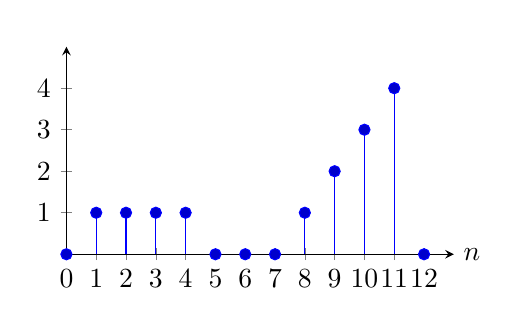
\begin{tikzpicture}
\begin{axis} [width=185pt,height=120pt,
	axis x line=bottom, 
	axis y line=middle, 
	tick align=center,
	every axis x label/.style={at={(current axis.right of origin)},anchor=west},
	every axis y label/.style={at={(current axis.above origin)}, anchor=north east,above=0mm},
	xmin=0, xmax=13,
	xtick={0,...,12},
	xlabel=$n$,
	ymin=0, ymax=5,
	ytick={0,...,4},
	ylabel={$\boldimgworld$}]
\addplot+[ycomb] 
coordinates {(0,0) (1,1) (2,1) (3,1) (4,1) (5,0) (6,0) (7,0) (8,1) (9,2)  (10,3)  (11,4)  (12,0)};
\end{axis}
\end{tikzpicture}
&~
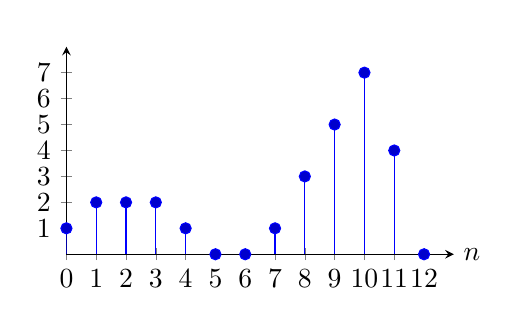
\begin{tikzpicture}
\begin{axis} [width=185pt,height=120pt,
	axis x line=bottom, 
	axis y line=middle, 
	tick align=center,
	every axis x label/.style={at={(current axis.right of origin)},anchor=west},
	every axis y label/.style={at={(current axis.above origin)}, anchor=north east,above=0mm},
	xmin=0, xmax=13,
	xtick={0,...,12},
	xlabel=$n$,
	ymin=0, ymax=8,
	ytick={0,...,7},
	ylabel={$\boldimgsensor$}]
\addplot+[ycomb] 
coordinates {(0,1) (1,2) (2,2) (3,2) (4,1) (5,0) (6,0) (7,1) (8,3) (9,5)  (10,7)  (11,4)  (12,0)};
\end{axis} 
\end{tikzpicture}
\end{array}
$
%\end{center}
}
\caption{Pinhole camera. (left) Input 1D signal, $\boldimgworld$. (right) The output of the two-pixel wide pinhole camera, $\boldimgsensor$.} 
\label{fig:2pixelwidepinhole}
\end{figure}

The output is obtained by multiplying the input vector by the matrix $\mathbf{A}$ shown in \fig{\ref{fig:amats1}}{d}. Each output value is the results of adding up two consecutive input values. The output is nearly identical to the input signal but with a larger magnitude and a bit smoother.

\section{More General Imagers}

Many different optical systems can form cameras and the linear analysis described before can be used to characterize the imaging process.  Even a simple edge will do.  \Fig{\ref{fig:amats3}} shows two non traditional imaging systems that we will analyze in this section. 


\begin{figure}[t]
\centerline{
\includegraphics[width=1\linewidth]{figures/imaging/nontraditional_pinholes_2.eps}
}
\caption{(a) Schematic drawing of an edge camera, and (b) its imaging matrices. (c) A pinspeck camera (an occluder that blocks two of the values on the scene), and (d) its imaging matrices.}
\label{fig:amats3}
\end{figure}

\subsection{Edge Camera}


Consider the example of \fig{\ref{fig:amats3}}{a}. This camera corresponds to an {\bf edge camera}\index{Camera!Edge camera}. This is not a traditional pinhole camera; instead light is blocked only on one side.  




For this camera, the imaging matrix and its inverse are as follows:
%\begin{equation}
%\mathbf{A} = 
%\left( 
%\begin{array}{ccccccccccccc}
%1 & 1 & 1 & 1 & 1 & 1 & 1 & 1 & 1 & 1 & 1 & 1 & 1 \\
%0 & 1 & 1 & 1 & 1 & 1 & 1 & 1 & 1 & 1 & 1 & 1 & 1 \\
%0 & 0 & 1 & 1 & 1 & 1 & 1 & 1 & 1 & 1 & 1 & 1 & 1 \\
%0 & 0 & 0 & 1 & 1 & 1 & 1 & 1 & 1 & 1 & 1 & 1 & 1 \\
%0 & 0 & 0 & 0 & 1 & 1 & 1 & 1 & 1 & 1 & 1 & 1 & 1 \\
%0 & 0 & 0 & 0 & 0 & 1 & 1 & 1 & 1 & 1 & 1 & 1 & 1 \\
%0 & 0 & 0 & 0 & 0 & 0 & 1 & 1 & 1 & 1 & 1 & 1 & 1 \\
%0 & 0 & 0 & 0 & 0 & 0 & 0 & 1 & 1 & 1 & 1 & 1 & 1 \\
%0 & 0 & 0 & 0 & 0 & 0 & 0 & 0 & 1 & 1 & 1 & 1 & 1 \\
%0 & 0 & 0 & 0 & 0 & 0 & 0 & 0 & 0 & 1 & 1 & 1 & 1 \\
%0 & 0 & 0 & 0 & 0 & 0 & 0 & 0 & 0 & 0 & 1 & 1 & 1 \\
%0 & 0 & 0 & 0 & 0 & 0 & 0 & 0 & 0 & 0 & 0 & 1 & 1 \\
%0 & 0 & 0 & 0 & 0 & 0 & 0 & 0 & 0 & 0 & 0 & 0 & 1 
%\end{array}
%\right) .
%\label{eq:edge}
%\end{equation}

\begin{equation}
\mathbf{A} = 
\left[ 
\begin{array}{cccccc}
1 & 1 & 1 & 1 & \dots & 1 \\
0 & 1 & 1 & 1 & ~ & 1 \\
0 & 0 & 1 & 1 & ~ & 1 \\
0 & 0 & 0 & 1 & ~ & 1 \\
\vdots & ~ & ~ & ~ & \ddots & ~ \\
0 & 0 & 0 & 0 & ~ & 1 
\end{array}
\right], 
\mathbf{A}^{-1} = 
\left[ 
\begin{array}{cccccc}
1 & -1 & 0 & 0 & \dots & 0 \\
0 & 1 & -1 & 0 & ~ & 0 \\
0 & 0 & 1 & -1 & ~ & 0 \\
0 & 0 & 0 & 1 & ~ & 0 \\
\vdots & ~ & ~ & ~ & \ddots & ~  \\
0 & 0 & 0 & 0 & ~ & 1 
\end{array}
\right]
\label{eq:edge}
\end{equation}

If we consider the same input as in the pinhole camera example in the previous section, the output signal for the corner camera will look like (\fig{\ref{fig:1dcornercamera}}):

\begin{figure}[h]
\centerline{
%\begin{center}
$
\begin{array}{cc}
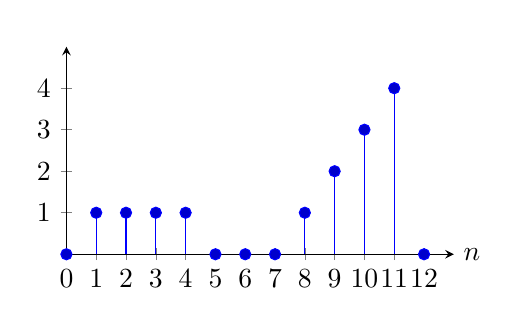
\begin{tikzpicture}
\begin{axis} [width=185pt,height=120pt,
	axis x line=bottom, 
	axis y line=middle, 
	tick align=center,
	every axis x label/.style={at={(current axis.right of origin)},anchor=west},
	every axis y label/.style={at={(current axis.above origin)}, anchor=north east,above=0mm},
	xmin=0, xmax=13,
	xtick={0,...,12},
	xlabel=$n$,
	ymin=0, ymax=5,
	ytick={0,...,4},
	ylabel={$\boldimgworld$}]
\addplot+[ycomb] 
coordinates {(0,0) (1,1) (2,1) (3,1) (4,1) (5,0) (6,0) (7,0) (8,1) (9,2)  (10,3)  (11,4)  (12,0)};
\end{axis}
\end{tikzpicture}
&~
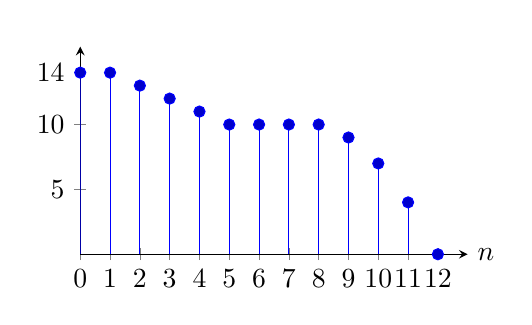
\begin{tikzpicture}
\begin{axis} [width=185pt,height=120pt,
	axis x line=bottom, 
	axis y line=middle, 
	tick align=center,
	every axis x label/.style={at={(current axis.right of origin)},anchor=west},
	every axis y label/.style={at={(current axis.above origin)}, anchor=north east,above=0mm},
	xmin=0, xmax=13,
	xtick={0,...,12},
	xlabel=$n$,
	ymin=0, ymax=16,
	ytick={0,5,10,14},
	ylabel={$\boldimgsensor$}]
\addplot+[ycomb] 
coordinates {(0,14) (1,14) (2,13) (3,12) (4,11) (5,10) (6,10) (7,10) (8,10) (9,9)  (10,7)  (11,4)  (12,0)};
\end{axis} 
\end{tikzpicture}
\end{array}
$
%\end{center}
}
\caption{Edge camera. (left) Input 1D signal, $\boldimgworld$. (right) The output of an edge camera, $\boldimgsensor$.} 
\label{fig:1dcornercamera}
\end{figure}

The output now looks very different than that of a pinhole camera. In the pinhole camera, the output is very similar to the input. This is not the case here where the output looks like the integral of the input (reversed along the horizontal axis). Note that the first value of $\boldimgsensor$ is equal to the sum of all the values of $\boldimgworld$:
\begin{equation}
\imgsensor \left[0 \right] = \sum_{n=0}^{12} \imgworld \left[n \right]
\end{equation}

\Fig{\ref{fig:amats3}}{b} illustrates the imaging matrix, $\mathbf{A}$, and reconstruction matrices for the imager of \eqn{\ref{eq:edge}}. You can think of this imager as computing an integral of the input signal. Therefore, its inverse looks like a derivative. The regularized inverse looks like a blurred derivative (we will talk more about blurred derivatives in \chap{\ref{chapter:image_derivatives}}).
%, as well as for an edge imager where the responses are blurred across several sensor elements.


\subsection{Pinspeck Camera}

\Fig{\ref{fig:amats3}}{c} shows another nontraditional imager. Now, instead of a pinhole we have an occluder. The occluder blocks part of the light (complementary to the large-hole pinhole camera shown in \fig{\ref{fig:amats1}}{c}). What the camera sensor records is the shadow of the occluder.
\marginnote{The shadow of an object is related to the negative of a picture taken of the environment around the object.}
We can write the imaging matrix $\mathbf{A}$, which corresponds to 1-$\mathbf{A}_{pinhole}$ as shown in \fig{\ref{fig:amats1}}{d}. \Fig{\ref{fig:amats3}}{d} also shows its inverse and the regularized inverse. This camera is called a {\bf pinspeck camera}\index{Camera!Pinspeck camera} \cite{CohenPinspeck,Torralba2014} and has also been used in practice. 

In the example of \fig{\ref{fig:amats3}}{c}, the occluder has the size of the wide pinhole from  \fig{\ref{fig:amats1}}{c}. The following plots shows, \fig{\ref{fig:pinspeck_output_plot}}{left}, the input scene (same as in the previous examples) and, \fig{\ref{fig:pinspeck_output_plot}}{right}, the output recorded by the camera sensor of the pinspeck camera. 
\begin{figure}
\centerline{
%\begin{center}
$
\begin{array}{cc}
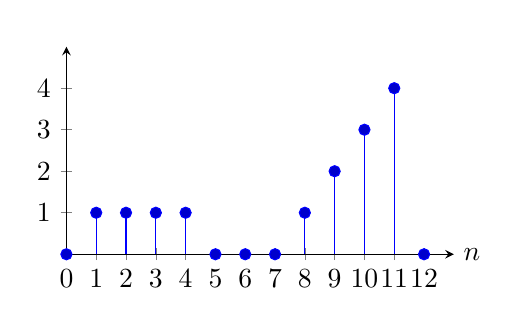
\begin{tikzpicture}
\begin{axis} [width=185pt,height=120pt,
	axis x line=bottom, 
	axis y line=middle, 
	tick align=center,
	every axis x label/.style={at={(current axis.right of origin)},anchor=west},
	every axis y label/.style={at={(current axis.above origin)}, anchor=north east,above=0mm},
	xmin=0, xmax=13,
	xtick={0,...,12},
	xlabel=$n$,
	ymin=0, ymax=5,
	ytick={0,...,4},
	ylabel={$\boldimgworld$}]
\addplot+[ycomb] 
coordinates {(0,0) (1,1) (2,1) (3,1) (4,1) (5,0) (6,0) (7,0) (8,1) (9,2)  (10,3)  (11,4)  (12,0)};
\end{axis}
\end{tikzpicture}
&~
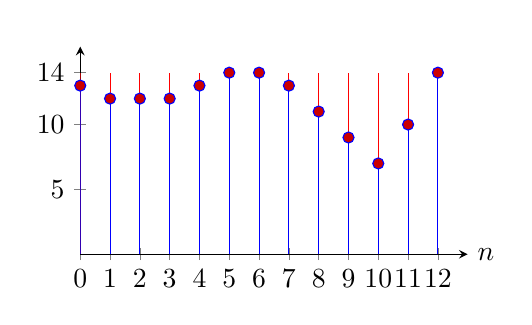
\begin{tikzpicture}
\begin{axis} [width=185pt,height=120pt,
	axis x line=bottom, 
	axis y line=middle, 
	tick align=center,
	every axis x label/.style={at={(current axis.right of origin)},anchor=west},
	every axis y label/.style={at={(current axis.above origin)}, anchor=north east,above=0mm},
	xmin=0, xmax=13,
	xtick={0,...,12},
	xlabel=$n$,
	ymin=0, ymax=16,
	ytick={0,5,10,14},
	ylabel={$\boldimgsensor$}]
\addplot[ycomb,red] 
coordinates {(0,14) (1,14) (2,14) (3,14) (4,14) (5,14) (6,14) (7,14) (8,14) (9,14)  (10,14)  (11,14)  (12,14)};
\addplot+[ycomb,blue,fill=blue,mark=*] 
coordinates {(0,13) (1,12) (2,12) (3,12) (4,13) (5,14) (6,14) (7,13) (8,11) (9,9)  (10,7)  (11,10)  (12,14)};
\end{axis} 
\end{tikzpicture}
\end{array}
$
%\end{center}
}
\caption{Pinspeck camera. (left) Input 1D signal, $\boldimgworld$. (right) The output of a pinspeck camera, $\boldimgsensor$.} 
\label{fig:pinspeck_output_plot}
\end{figure}

The output is now a signal with a wide dynamic range (a max value of 14, which correspond to the sum of the values in $\boldimgworld$) and with fluctuations due to the shadow of the occluder on the camera sensor. If there was no occluder, then the output would be a constant signal of value 14. In red we show the effect of the shadow, which is the light missing because of the presence of the occluder. You can see how the missing signal is identical to the output of the two-pixel wide pinhole camera but reversed in sign.


%\begin{figure}
%\centerline{
%\sublabel{a}{\includegraphics[width=0.45\linewidth]{figures/imaging/ph3.pdf}}}
%\centerline{
%\sublabel{b}{\includegraphics[width=0.45\linewidth]{figures/imaging/amat31.pdf}}
%\sublabel{c}{\includegraphics[width=0.45\linewidth]{figures/imaging/amat34.pdf}}
%}
%\caption{
%(a) An edge camera (b) Visualization of idealized imaging matrices:  The imaging matrix relating scene intensities to sensor readings; the inverse of that matrix;  the regularized inverse.  (c) A blurred edge imaging matrix, and its inverse and regularized inverse }
%\label{fig:amats3}
%\end{figure}





\subsection{Corner Camera}  

To show a real-world example of a more general imager, let us consider the {\bf corner camera}\index{Camera!Corner camera} \cite{Bouman17}.  This is similar to the edge
camera of \eqn{\ref{eq:edge}} and \fig{\ref{fig:amats3}}, but with
slightly more complicated geometry.  As shown in
\fig{\ref{fig:ccmodel}}{a}, a vertical edge partially blocks a scene from view, creating intensity variations on the ground, observable by viewing those intensity variations from around the corner.


\begin{figure}[t]
\centerline{
\sublabel{a}
{\includegraphics[width=0.4\linewidth]{figures/imaging/cornercam.pdf}}
\sublabel{b}
{\includegraphics[width=0.4\linewidth]{figures/imaging/cornerKey.pdf}}}
\caption{The corner camera \cite{Bouman17}.  (a) Objects, such as the cylinders labeled A and B, hidden behind a corner from a camera nonetheless cause a very small intensity differences in the ambient illumination falling on the ground.
%, observable from the camera as a very small change in the light intensity reflecting from the ground.  The image reconstruction operation is analogous to that for the edge camera of \fig{\ref{fig:amats3}}:  we subtract the reflected intensities observed at one orientation angle, say $\theta_A$ from those observed at another, say $\theta_B$. 
(b) the spatial mask is multiplied by the observed reflected ground image.}
\label{fig:ccmodel}
\end{figure}


In practice, we will subtract a mean image from our observations of the ground plane, so in the rendering equation below, we will only consider components of
the scene that may change over time, under the assumption that what we want to image behind the corner (e.g., a person) is moving.  We will call these intensities
$S(\phi, \theta)$ ($S$ for the subject), where $\phi$ measures
vertical inclination and $\theta$ measures azimuthal angle, relative to position where the vertical edge intersects the ground plane.  Integrating the light intensities falling on the ground plane, the
observed intensities on the ground will be $\boldimgground (r, \theta)$, where the
polar coordinates $r$ and $\theta$ are measured with respect to the corner.
Assuming Lambertian diffuse reflection from the ground plane, we have, for the observed intensities $\boldimgground (r, \theta)$,
\begin{equation}
 \boldimgground (r, \theta) = \int_{\phi=0}^{\phi=\pi} \int_{\xi=0}^{\xi=\theta}
 \cos(\phi) S(\phi, \xi) \mbox{d} \phi \mbox{d} \xi,
\label{eq:corner}
\end{equation}
where the $\cos(\phi)$ term in \eqn{\ref{eq:corner}} follows from the equation for surface reflection, \eqn{\ref{eq:lambert}}.



The dependence of the observation, $\boldimgground$, on vertical variations in
$S(\phi, \theta)$ is very weak, just through the $\cos(\phi)$ term.
We can integrate over $\phi$ first, to form the 1D signal,
$\imgworld (\xi)$:
\begin{equation}
  \imgworld (\xi) = \int_{\phi=0}^{\phi=\pi} 
  \cos(\phi) S(\phi, \xi) \mbox{d} \phi 
\label{eq:xcorner}
\end{equation}

Then, to a good approximation, \eqn{\ref{eq:corner}} has the form,
\begin{equation}
 \boldimgground (r, \theta) \approx \int_{\xi=0}^{\xi=\theta}
 \imgworld (\xi) \mbox{d} \xi,
\label{eq:corner1d}
\end{equation}
where $\imgworld (\xi)$ is a 1D image of the scene around the corner from the vertical edge.

\Fig{\ref{fig:ccmodel}} shows the corner camera geometry for a three-dimensional (3D) scene.  \Fig{\ref{fig:ccmodel}}{a} shows two objects, such as the cylinders labeled A and B, hidden behind a corner from a camera. Despite being behind the corner they cause a very small intensity differences in the ambient illumination falling on the ground, observable from the camera as a very small change in the light intensity reflecting from the ground. Can we reconstruct the scene hidden behind the corner using just the intensities observed on the ground? The image reconstruction operation is analogous to that for the edge camera of \fig{\ref{fig:amats3}}:  we subtract the reflected intensities observed at one orientation angle, say $\theta_A$ from those observed at another, say $\theta_B$. 

If we sample \eqn{\ref{eq:corner1d}} in its continuous variables, we
can write it in the form $\boldimgground = \mathbf{A} \boldimgworld$.  Solving \eqn{\ref{eq:deriv2}}
for the multiplier to apply to $\boldimgground$ to estimate $\boldimgworld$ yields the form shown in
\fig{\ref{fig:ccmodel}}{b}.  \Fig{\ref{fig:ccmodel}}{b} shows the spatial mask to be multiplied by the observed reflected ground image, with the result summed over all spatial pixels in order to estimate the light coming from around the corner at one particular orientation angle relative to the corner, in this case approximately 45 degrees. We see that the way to read the 1D signal from the ground plane is to take a derivative with respect to angle.  This makes intuitive sense, as the light intensities on the ground integrate all the light up to the angle of the vertical edge.  To find the 1D signal at the angle of the edge, we ask, ``What does one pie-shaped ray from the wall see that the pie-shaped ray next to it doesn't see?''


It can be shown \cite{Bouman17} that the image intensities from around-the-corner scenes introduce a perturbation of about $\frac{1}{1,000}$ to the light reflected from the ground from all sources.   
By averaging image intensities over the appropriate pie-shaped regions on the ground at the corner (\fig{\ref{fig:ccmodel}}[b]), one can extract a 1D image as a function of time from the scene around the corner.  \Fig{\ref{fig:cctraces}} shows two 1D videos reconstructed from one (\fig{\ref{fig:cctraces}}[a]) and two (\fig{\ref{fig:cctraces}}[b]) people walking around the corner.  By processing videos of very faint intensity changes on the ground, we can infer a 1D video of the scene around the corner.  The image inversion formulas were derived using inversion methods very similar to \eqn{\ref{eq:deriv2}}.  The corner camera is just one of the many possible instantiations of a computational imaging system.


\begin{figure}[t]
\centerline{
\includegraphics[width=0.9\linewidth]{figures/imaging/corner_camera_3D.eps}
}
%\centerline{
%\sublabel{a}
%{\includegraphics[width=0.4\linewidth]{figures/imaging/corner.jpg}}
%\sublabel{b}
%{\includegraphics[width=0.4\linewidth]{figures/imaging/2people.jpg}}}
%\centerline{
%\sublabel{c}
%{\includegraphics[width=0.2\linewidth]{figures/imaging/cctrace.pdf}}
%\sublabel{d}
%{\includegraphics[width=0.2\linewidth]{figures/imaging/cctrace2.pdf}}
%}
\caption{Outdoor corner camera \cite{Bouman17} experiments. (a) Camera recording ground plane intensities.  (b) Two people walking around the corner, hidden from direct view of the camera. (c) Corner camera trace with one person moving. (d) Corner camera trace with two people moving.  Angle from the corner is plotted vertically, and time is plotted horizontally.}
\label{fig:cctraces}
\end{figure}

\marginnote{People moving out of view around a corner cause small, invisible changes in the light reflecting from the ground. These faint changes occur at nearly every corner and can be used to read-out 1D images of the people around the corner.}[0in]


%% 
%% \subsection{Pinhole lightfield imager}
%% An array of pinholes.  How to construct and photograph that?
%% 


\section{Concluding Remarks}  
Treating cameras as general linear systems allows for the machinery of linear algebra to be applied to camera design and processing.  We reviewed several simple camera systems, including cameras utilizing pinholes, pinspecks, and edges to form images.
 % Bill
% \chapter{Camera Modeling and Calibration}
%\section{Camera model}
\label{sec:camera_parameters}


\section{Introduction}

In \chap{\ref{chapter:imaging}} we described the image formation process assuming that the camera was the central element and we placed the origin of the world coordinates system in the pinhole. But, as we will be interested in interpreting the scene in front of the camera, other systems of reference might be more appropriate. For instance, in the simple world model of \chap{\ref{chapter:simplesystem}} we placed the origin of the world coordinates system on the ground, away from the camera. What formulation of the image formation process will allow us changing coordinate systems easily? This is what we will study in this chapter. 

In the sketch shown below (\fig{\ref{fig:world_and_camera_coordinates}}), a standing person is holding a camera and taking a picture with it of someone sitting at a table (sorry for our drawing skills but hopefully this description compensates for our poor artistry). We will be answering questions about the scene based on the picture taken by the camera: for instance, how high and large is the table?  We will also answer questions about the camera, like how high is the camera above the floor? 

\begin{figure}[h]
\centerline{
\includegraphics[width=1\linewidth]{figures/imaging_geometry/world_and_camera_coordinates.eps}
}
\caption{Camera-centric and world-centric camera coordinate systems.}
\label{fig:world_and_camera_coordinates}
\end{figure}

In settings where we have multiple cameras we will have to be able to transform the coordinates frames between cameras. And finally, to translate the two-dimensional (2D) images into the underlying three-dimensional (3D) scene, we need to know how 2D points relate to 3D world coordinates, which is called calibrating the cameras.
 
In this chapter we will show how to use homogeneous coordinates to describe a camera projection model that is more general than what we have done until now. This formulation will be key to building most of the approaches we will study from now until the end of this book; therefore it is important to be familiar with it. It is also often used both in classic computer vision approaches and in deep learning architectures. 

But before we move into the material, we are sure you would like to see the picture that the standing character from the previous sketch took. Here it is:

\begin{figure}[h]
\centerline{
\includegraphics[width=.25\linewidth]{figures/imaging_geometry/the_picture.eps}
}
\caption{The picture taken by the standing character from \fig{\ref{fig:world_and_camera_coordinates}}.}
\end{figure}


\section{3D Camera Projections in Homogeneous Coordinates}

Let's start this chapter with the most important application of homogeneous coordinates for us: describing perspective projection. For now, we will continue assuming that the origin of the world coordinates system is at the pinhole location and that the $Z$-axis corresponds to the optical axis (i.e., it is perpendicular to the image plane).

%As we have already discussed (see \fig{\ref{ig:pinholeGeometry2bis}} to refresh your memory), the perspective projection equations relating camera pixel position, $[x,y]^\transpose$, of the image of a point to the point's world 3D position, $([X,Y,Z]^\transpose$, involve division by the point's $Z$-location, as $x=f \, X/Z$ and $y=f\, Y/Z$.  This division complicates algebraic relations. Projective geometry and homogeneous coordinates are tools that simplify those algebraic relations, and thus simplify many of the equations that involve geometric transformations.


As we have already discussed (see \fig{\ref{fig:pinholeGeometry2bis}} to refresh your memory), the perspective projection equations are nonlinear and involve a division by the point's $Z$-location. That is, a 3D point with coordinates $[X,Y,Z]^\transpose$ appears in the image at coordinates $[x,y]^\transpose$ where $x=f \, X/Z$ and $y=f\, Y/Z$ ($f$ is the focal length). This division complicates algebraic relations. Projective geometry and homogeneous coordinates are tools that simplify those algebraic relations, and thus simplify many of the equations that involve geometric transformations.

%relating camera pixel position, $[x,y]^\transpose$, of the image of a point to the point's world 3D position, $([X,Y,Z]^\transpose$, involve division by the point's $Z$-location, as $x=f \, X/Z$ and $y=f\, Y/Z$. 


\begin{figure}[h]
\centerline{
%\includegraphics[width=.8\linewidth]{figures/imaging/pinholeGeomGumby.jpg}
\includegraphics[width=0.8\linewidth]{figures/imaging_geometry/camera_centric.eps}
}
\caption{Perspective projection. Remember that from similar triangles, we have $x/f = X/Z$ and $y/f = Y/Z$.}
\label{fig:pinholeGeometry2bis}
\end{figure}



To write points in 3D space in homogeneous coordinates, we add a fourth coordinate to the three coordinates of Euclidean space, as described in \chap{\ref{chapter:geometry_homogeneous}}.
%with the same scaling rules applying as for the case of 2D homogeneous coordinates.
Using homogeneous coordinates, camera projections can be written in a simple form as a matrix multiplication.  Consider a coordinate system with the origin fixed at the center of projection of the camera and the 3D point in homogeneous coordinates, $\mathbf{P}=[X, Y, Z, 1]^\transpose$.

We can verify that the matrix, $\mathbf{K}$, shown below, multiplied by the vector describing the 3D point, $\mathbf{P}$, returns the position of its perspective projection (equation [\ref{eq:perspctiveProj}]):
\begin{eqnarray}
    \mathbf{K} \mathbf{P} & = &
    \begin{bmatrix}
    f & 0 & 0 & 0 \\
    0 & f & 0 & 0 \\
    0 & 0 & 1 & 0
    \end{bmatrix}
    \begin{bmatrix}
    X \\
    Y \\
    Z \\
    1
    \end{bmatrix}
     = 
    \begin{bmatrix}
    f X \\
    f Y \\
    Z
    \end{bmatrix}
    =
    \lambda
    \begin{bmatrix}
    x \\
    y \\
    1
    \end{bmatrix}
\end{eqnarray}
Transforming the product vector from homogeneous coordinates to heterogeneous coordinates yields
\begin{equation}
    \begin{bmatrix}
    f X \\
    f Y \\
    Z
    \end{bmatrix}
    \rightarrow
    \begin{pmatrix}
    f X/Z \\
    f Y/Z
    \end{pmatrix}
    =
    \begin{pmatrix}{c}
    x \\
    y
    \end{pmatrix}
    =
    \mathbf{p}
\end{equation}
showing that the matrix $\mathbf{K}$, when multiplied by the homogeneous coordinates of a 3D point, $\mathbf{P}$, renders the homogeneous coordinates of the perspective projection of that 3D point, $\mathbf{p}$. This formulation is one of the biggest benefits of using homogeneous coordinates. It allows writing perspective projection as a linear operator in homogeneous coordinates.

Because homogeneous coordinates, and therefore also the transformation matrices, are only defined up to an arbitrary uniform (non zero) scale factor, the perspective projection transformation matrix is equivalently written as
\begin{equation}
    \mathbf{K} =             
    \begin{bmatrix}
    1 & 0 & 0 & 0 \\
    0 & 1 & 0 & 0 \\
    0 & 0 & 1/f & 0
    \end{bmatrix}
    \label{eq:homogPerspective}
\end{equation}
Also, in this particular case, it is fine to drop the last column of $\mathbf{K}$ and use the heterogeneous coordinates form of $\mathbf{P}$. However, it is interesting to keep the homogeneous formulation, as it will allow us to work with more general forms of camera models, as we will see next. 



\subsection{Parallel Projection}

We can use homogeneous coordinates to describe a wide variety of camera models.
For instance, the projection matrix for an orthographic projection (equation [\ref{eq:orthographicProj}]), $\mathbf{K}$, is
\begin{equation}
\mathbf{K} =         
    \begin{bmatrix}
    1 & 0 & 0 & 0 \\
    0 & 1 & 0 & 0 \\
    0 & 0 & 0 & 1
    \end{bmatrix}
    ,
    \label{eq:parallel_projection_matrix}
\end{equation}
as can be verified by multiplying by a 3D point in homogeneous coordinates.


\section{Camera-Intrinsic Parameters}

%Now that we have seen how 3D to 2D projection can be modeled using homogeneous coordinates and very simple vector computations, how can we use this to model cameras? We want a

%Cameras will output pixels and there might be other factors such as geometric distortions that will affect the relationship between the 3D scene and the image captured by the camera. 

Now that we have seen how 3D to 2D projection can be effectively modeled using homogeneous coordinates and simple vector computations, let's apply these tools to model cameras.

We want to construct a camera model that captures the image formation process. Cameras translate the world into pixels, but the relationship between the 3D scene and the 2D image captured by the camera is not always straightforward. To start with, the world is measured in units of meters while points in images are measured in pixels. Factors such as geometric distortions can influence this relationship, and we need to account for these elements in our camera model.

\subsection{From Meters to Pixels}

\Fig{\ref{fig:pinhole_and_sensor}} illustrates the image formation process and the image sampling by the sensor. 
We need to account for the perspective projection of the point, $\mathbf{P}$, described in camera coordinates, to pixel coordinates in the sensor plane of the camera.  

\begin{figure}[t]
\centerline{
\includegraphics[width=1\linewidth]{figures/imaging_geometry/pinhole_and_sensor.eps}
}
\caption{An image is projected into the sensor. World coordinates are transformed into pixels at the sensor. The focal length is $f$, and the physical width of the sensor is $w$. The sensor has $N \times M$ pixels.}
\label{fig:pinhole_and_sensor}
\end{figure}



The units of the position in pixel space may be different than those of the world coordinates, which scales the focal length, $f$, in \eqn{\ref{eq:homogPerspective}} to some other value. Let's call that value $a$:
\begin{equation}
    \mathbf{K} =             
    \begin{bmatrix}
    a & 0 & 0 & 0 \\
    0 & a & 0 & 0 \\
    0 & 0 & 1 & 0
    \end{bmatrix}
    \label{eq:intrinsic}
\end{equation}
where the constant $a$ is related to the physical camera parameters in the following way:
\begin{equation}
a = f \, N / w
\end{equation}
where $f$ is the focal length (in meters), $w$ is the width of the sensor in meters, and $N$ is the image width in pixels. The ratio $N/w$ is the number of pixels per meter in the sensor.

Also, the image center might not be the pixel $[0,0]^\transpose$. If the optical axis coincides with the image center, we need to apply a translation so that a 3D point on the optical axis (i.e., $X=Y=0$) projects to $[c_x, c_y]^\transpose$. For example, for an image of size $N \times M$ we will have $c_x=N/2$ and $c_y=M/2$:
\begin{equation}
    \mathbf{K} =             
    \begin{bmatrix}
    a & 0 & c_x & 0 \\
    0 & a & c_y & 0 \\
    0 & 0 & 1 & 0
    \end{bmatrix}
    \label{eq:intrinsic}
\end{equation}
It is also possible that the pixels are not square, in which case we have to account for different scaling along both axis:
\begin{equation}
    \mathbf{K} =             
    \begin{bmatrix}
    a & 0 & c_x & 0 \\
    0 & b & c_y & 0 \\
    0 & 0 & 1 & 0
    \end{bmatrix}
    \label{eq:intrinsic}
\end{equation}
Then, the final transformation from 3D coordinates, $[X,Y,Z]^\transpose$, to image pixels, $[n,m]^\transpose$, has the form: 
\begin{equation}
    \begin{bmatrix}
    a & 0 & c_x & 0 \\
    0 & b & c_y & 0 \\
    0 & 0 & 1 & 0
    \end{bmatrix}
    \begin{bmatrix}
    X \\
    Y \\
    Z \\
    1
    \end{bmatrix}
    \rightarrow
    \begin{pmatrix}
    a X/Z+c_x \\
    b Y/Z+c_y
    \end{pmatrix}
    =
    \begin{pmatrix}
    n \\
    m
    \end{pmatrix}
    \label{eq:intrinsic}
\end{equation}




The signs of $a$ and $b$ can be positive or negative. With the convention used in this book, where the camera optical axis coincides with the $Z$-axis and the camera looks in the direction of positive $Z$, the sign of $a$ has to be negative. If $n$ and $m$ are indices into an array, then the image origin is located at the top-left of the array, which means the signs of $a$ and $b$ will be negative. This is the convention used by Python and OpenCV. \Fig{\ref{fig:conventions}} shows two different common conventions. 


\begin{figure}[t]
\centerline{
\includegraphics[width=1\linewidth]{figures/imaging_geometry/conventions_coordinates.eps}
}
\caption{(a) 3D representation of the image plane. 
(b and c) Two different conventions for the image coordinate systems. In this book we have been using (b).}
\label{fig:conventions}
\end{figure}


\subsection{From Pixels to Rays}
\label{sec:pixel_to_rays}

If you have a calibrated camera, can we derive the equation of the ray that leaves the image at one point? Answering this question, will allow us answering the following one: If we know $Z$ for an image pixel with camera-coordinates $x,y$, can get the point world-coordinates $X$ and $Y$? 

We can relate the point in the image plane, $\mathbf{p}$, with the 3D point $\mathbf{P}$ in world-coordinates. To do this, we will first play a little trick: We will express the 2D point $\mathbf{p}$ in 3D coordinates. We can do this by realizing that the point $\mathbf{p}$ is contained in the image plane which is located at a distance $f$ of the origin along the $Z$-axis (\fig{\ref{fig:coordinate_systems_ray}}).
%, also describing $\mathbf{p}$ also using the 3D coordinates. 
Therefore, in 3D, the 2D point $\mathbf{p}$ is a point located at coordinates $Z_c=f$, where $f$ is the focal length, $X_c=x$, and $Y_c=y$, as illustrated in \fig{\ref{fig:coordinate_systems_ray}}.
%\begin{equation}
%    %\mathbf{p} = 
%    \left (
%    \begin{array}{c}
%    x\\
%    y \\
%    f
%    \end{array}
%    \right )
%\end{equation}


\begin{figure}[h]
\centerline{
%\includegraphics[width=.8\linewidth]{figures/imaging/pinholeGeomGumby.jpg}
\includegraphics[width=0.75\linewidth]{figures/imaging_geometry/light_ray.eps}
}
\caption{The 3D point $\mathbf{P}$ is obtained by scaling the point $\mathbf{p}=(x,y,f)$ with a scaling factor $Z/f$. The ray that passes by the point $\mathbf{p}$ is the line defined by $\lambda (x,y,f)$, with $\lambda$ being a positive real number.}
\label{fig:coordinate_systems_ray}
\end{figure}

The ray that connects the camera center and the point $\mathbf{p}$ is $\lambda (x,y,f)$, with $\lambda$ being a positive real number. Any 3D point along this line will project into the same image point $\mathbf{p}$ under perspective projection. 

As shown in \fig{\ref{fig:coordinate_systems_ray}} the 3D point $\mathbf{P}$ is obtained by scaling the ray that passes by $\mathbf{p}$. The scaling factor is $\lambda = Z/f$:
\begin{equation}
    \frac{Z}{f}
    \begin{pmatrix}
    x\\
    y\\
    f
    \end{pmatrix}
    =
    \begin{pmatrix}
    X \\
    Y \\
    Z
    \end{pmatrix}
\end{equation}

%By changing the value of $Z$ we have the ray that passes by $\mathbf{p}$. 
We should use $a$ instead of $f$ if we are using coordinates in pixels. We will revisit this again in \chap{\ref{chapter:3D_learning_from_single_image}}.


\subsection{A Simple, although Unreliable, Calibration Method}
\label{sec:simple_unreliable_calibration_method}

Everything we described up to here, relies on a series of parameters (i.e., focal length, sensor size) that will be unknown in general. Before we continue, let's try to see if we can find out what those parameters are in a real setting. 

Let's start by describing a simple and intuitive method for camera calibration illustrated in \fig{\ref{fig:simple_calibration}}. The method we will describe is not very accurate, but it provides be a good sanity check before doing more precise camera calibrations. We will describe a more accurate method in \sect{\ref{sec:camera_calibration}}.


\begin{figure}[h]
\centerline{
\sublabel{a}{\includegraphics[width=.62\linewidth]{figures/imaging_geometry/simple_calibration_1.jpg}}
%~
\sublabel{b}{\includegraphics[width=.33\linewidth]{figures/imaging_geometry/simple_calibration_2.jpg}}
}
\caption{A simple calibration setting.}
\label{fig:simple_calibration}
\end{figure}

To calibrate a camera we need the following three ingredients: 
\begin{itemize}
\item An object of known size: In this setting, \fig{\ref{fig:simple_calibration}}{a}, the object is a $8\times10$ chessboard pattern printed so that each square exactly measures 2 $\times$ 2 cm. The total width is $W=20$ cm. This chessboard is a standard calibration target \cite{Zhang1999}. 
\item The distance between the camera and the object: We use a ruler to measure that the distance between the camera and the chessboard as shown in \fig{\ref{fig:simple_calibration}}{a}. The distance is approximately $Z=31$ cm.
\item A picture of the object: \Fig{\ref{fig:simple_calibration}}{b} shows the picture taken by the camera shown in \fig{\ref{fig:simple_calibration}}{a}. The camera plane is parallel to the chessboard. From the picture, we can measure the width of the chessboard in pixels, which is $L=2{,}002$ pixels. 
\end{itemize}
These three quantities, $W$, $L$ and $Z$, are related via the parameter $a$ of the projection matrix by the equation: $a= Z L/W$, which results in:
\begin{equation}
a = \frac{31 \times 2{,}002}{20} = 3{,}103.1
\end{equation}

%to take a picture of an object of a known size from a known distance and use the size of the object measured on the image to calculate the camera parameters. The following image shows an example of this calibration setting:

% https://www.analyticsvidhya.com/blog/2021/10/a-comprehensive-guide-for-camera-calibration-in-computer-vision/





%In this setting, \fig{\ref{fig:simple_calibration}}, the object is a $8\times10$ checkerboard pattern printed so that each square exactly measures 2cm $\times$ 2cm. The picture is taken with a phone camera placed so that the camera plane is parallel to the checkerboard.
% https://forums.macrumors.com/threads/flagship-camera-comparison-13-pro-12-pro-max-12-pro-11-pro-xs-x.2311859/?fr=operanews

%\marginnote{Geometry corresponding to \fig{\ref{fig:simple_calibration}}:\\
%\centerline{
%\includegraphics[width=1\linewidth]{figures/imaging_geometry/calibration_a.eps}}
%}
%The left image in \fig{\ref{fig:simple_calibration}} shows the overall configuration were the phone is used to take a picture of a calibration board. The intrinsic parameter $a$ can be estimated as $a= Z L/W$ where $Z$ is the distance to the board, $W$ is the board width and $L$ is the width of the board in pixels in the picture. The board is a checkerboard with a width of 20cm. The camera is approximately fronto-parallel to the board and at a distance of 31cm to it.  

The picture size is $4{,}032 \times 3{,}024$ pixels which we can use to get the other two parameters of the camera projection matrix: $c_x=3{,}024/2$ and $c_y=4{,}032/2$. Putting all together we get the projection matrix:

\begin{equation}
    \mathbf{K} =             
    \begin{bmatrix}
    3{,}103.1 & 0 & 1{,}512 & 0 \\
    0 & 3{,}103.1 & 2{,}016 & 0 \\
    0 & 0 & 1 & 0
    \end{bmatrix}
    \label{eq:intrinsic}
\end{equation}

Would it be possible to infer the intrisic camera matrix from the camera technical specifications alone?  Can we directly estimate the parameter $a$ directly from the camera specs? The picture is taken with the wide-angle lens of an iPhone 13 pro. The focal length is 5.7 mm, the sensor size is $7.6 \times 5.7$ mm, and the image size is $4{,}032 \times 3{,}024$ pixels. This gives as an intrinsic parameter of:
\begin{equation}
a = \frac{4{,}032 \times 5.7}{7.6} = 3{,}024. 
\end{equation}
It works! (Does it?) Or at least it is close. But a lot of things happen inside a camera and estimating these values from hardware specs might be difficult.

But is this quality for the calibration enough? 


\subsection{Other Camera Parameters}

Unfortunately, there are other important aspects of a camera that require precise calibration. In some rare cases, pixels might not be square, or might be arranged along non-perpendicular axes, which requires introducing a skew parameter in $\mathbf{K}$. 
Radial distortion introduced by lenses is often an important and frequent source of issues that requires calibration. When there is radial distortion, straight lines will appear curved. In that case, it is very important to correct for the distortion. Standardized tools for camera calibrations take into account all these different aspects of the camera in order to build an accurate camera model. A more in-depth description of these tools and methods can be found here \cite{Zhang1999,Zhang2000}.



%\section{Camera model}
\section{Camera-Extrinsic Parameters}

In all our previous examples, we have been assuming that the camera origin was located at the origin of the world coordinate system with the optical axis aligned with the world $Z$-axis. In practice, there will be many situations where placing the camera at a special position will be more convenient. For instance, in the simple vision system we studied in chapter \ref{chapter:simplesystem} the camera center was placed above the $Z$-axis. Let's now study a more general setup where the camera is placed at an arbitrary location away from the world coordinate system. 

In the examples shown in \fig{\ref{fig:camera_calibration}}, we are interested in placing the world coordinate system so that the origin is on the ground and the axes $Z_w$ and $X_W$ are contained on the ground plane, and parallel to the two axis defined by the table. The axis $Y_W$ is perpendicular to the ground. Let's say that our camera has its camera center displaced by vector $\mathbf{T}$ and the axes are rotated by $\mathbf{R}^\transpose$ with respect to the world-coordinates system, as shown in \fig{\ref{fig:camera_calibration}}. Precisely, this is done by first placing the camera at the origin of the world-coordinates system, then rotating the camera with the rotation matrix $\mathbf{R}^\transpose$ and finally translating it by $\mathbf{T}$ (the order of these two operations matters). We use the inverse of $\mathbf{R}$ (equal to its transpose) to simplify the derivations later. 



\begin{figure}[t]
\centerline{
\includegraphics[width=0.7\linewidth]{figures/imaging_geometry/world_and_camera_coordinates_2.eps}
}
\caption{World- and camera-coordinate systems. A 3D point expressed in world coordinates, $\mathbf{P}_W$, can be expressed in the camera-coordinate frame, $\mathbf{P}_c$, by applying the translation, $\mathbf{T}$, and rotation, $\mathbf{R}$, to the point coordinates.}
\label{fig:camera_calibration}
\end{figure}

We are now given a point in the world $\mathbf{P}_W$, with its coordinates are described in terms of the world-coordinate system. Our goal is to find how that point projects into the image captured by the camera. To do this, first we need to change the coordinate system and express the point with respect to the camera coordinate system. Once we have done that change of coordinate system, we can use the intrinsic camera model $K$ to project the point into the image plane.  


%In order to compute the projection of this point into the camera we will do this in two steps.



%We need to translate, and then to rotate the camera so that points in the world, $\mathbf{P}_W$, are written in terms of a coordinate system with its origin at the camera center, and rotated to align with the camera (note that the order is reverse to how we defined the camera coordinate system earlier in this section). 

We need to initially translate, and subsequently rotate, the camera so that points in the world, $\mathbf{P}_W$, are expressed in a coordinate system that originates at the camera center and is rotated to align with the camera. Note that this order is reversed from how we defined the camera coordinate system earlier in this section. Using heterogeneous coordinates we can describe these two transformations as:

\begin{equation}
\mathbf{P}_C = \mathbf{R} (\mathbf{P}_W  - \mathbf{T}) = \mathbf{R} \mathbf{P}_W  -  \mathbf{R}\mathbf{T}
\end{equation}
where we use the $3\times3$ matrix, $\mathbf{R}$, to rotate the camera so that the camera's coordinates are parallel to those of the world. The vector $\mathbf{T}$ is the position of the camera in world coordinates. The rotation $\mathbf{R}$ in this equation is the inverse of the rotation matrix of the camera coordinate system with respect to the world coordinates.

%If we do translation and then rotation we would get $\mathbf{R} ( \mathbf{P}_W  - \mathbf{T})$. 



Let's use now homogeneous coordinates to describe the transformation from world coordinates to camera coordinates. To do so, we first translate the coordinate system by $-\mathbf{T}$ using the homogeneous matrix, $\mathbf{M}_1$:

\begin{equation}
\mathbf{M}_1 =         
    \begin{bmatrix}
    1 & 0 & 0 & -T_X \\
    0 & 1 & 0 & -T_Y \\
    0 & 0 & 1 & -T_Z \\
    0 & 0 & 0 & 1
    \end{bmatrix}
\end{equation}

Then, we use the $3\times 3$ matrix, $\mathbf{R}$, to rotate the camera so that the camera's coordinates are parallel to those of the world:
\begin{equation}
\mathbf{M}_2 =         
    \begin{bmatrix}
    R_1 & R_2 & R_3  & 0 \\
    R_4 & R_5 & R_6 & 0 \\
    R_7 & R_8 & R_9 & 0 \\
    0 & 0 & 0 & 1
    \end{bmatrix}
    \label{eq:homographyRotation}
\end{equation}


Using these two matrices we have
\begin{equation}
\mathbf{P}_C = \mathbf{M}_2 \mathbf{M}_1 \mathbf{P}_W
\label{eq:extrinsic}
\end{equation}
where $\mathbf{P}_W$ and $\mathbf{P}_C$ are the 3D coordinates of the same point (\fig{\ref{fig:camera_calibration}}), written in world and camera coordinates, respectively. Sometimes, this transformation is written by making the product of the two matrices explicit:

\begin{equation}
\mathbf{M}_2 \mathbf{M}_1=         
    \begin{bmatrix}
    R_1 & R_2 & R_3  & -\mathbf{r}_1 \mathbf{T} \\
    R_4 & R_5 & R_6 & - \mathbf{r}_2 \mathbf{T} \\
    R_7 & R_8 & R_9 & - \mathbf{r}_3 \mathbf{T} \\
    0 & 0 & 0 & 1
    \end{bmatrix}
    =
    \begin{bmatrix}
    \mathbf{R} & -\mathbf{R}\mathbf{T} \\
    \mathbf{0}^\transpose & 1
    \end{bmatrix}
\label{eq:extrinsic2}
\end{equation}
where $\mathbf{r}_i$ represents the row $i$ of the rotation matrix $\mathbf{R}$. 

Substituting \eqn{\ref{eq:extrinsic2}} into \eqn{\ref{eq:extrinsic}} we can now translate a 3D point expressed in world coordinates into camera coordinates:
\begin{equation}
\mathbf{P}_C = 
    \begin{bmatrix}
    \mathbf{R} & -\mathbf{R}\mathbf{T} \\
    \mathbf{0}^\transpose & 1
    \end{bmatrix}
    \mathbf{P}_W
%\label{eq:extrinsic}
\end{equation}

The camera parameters, $\mathbf{R}$ and $\mathbf{T}$, that relate the camera to the world are called the {\bf extrinsic camera parameters}. These parameters are external to the camera. 

We have seen now how to transform a point described in the world-coordinate system into the camera-coordinates system. We can now use the intrinsic camera parameters to project the point into the image plane. In the next section we will see how to combine both sets of parameters to get a full camera model. 



\section{Full Camera Model}

The concatenation of the extrinsic and intrinsic transformation matrices yields the desired transformation matrix, which will transform world coordinates to rendered pixel coordinates:
\begin{equation}
    \lambda
    \begin{bmatrix}
    x \\
    y \\
    1
    \end{bmatrix}
    =
    \begin{bmatrix}
    x' \\
    y' \\
    w
    \end{bmatrix}
=
\mathbf{K} \mathbf{M}_2 \mathbf{M}_1 
    \begin{bmatrix}
    X \\
    Y \\
    Z \\
    1
    \end{bmatrix}
    \label{eq:combined}
\end{equation}
Converting back to heterogeneous from homogeneous coordinates, the 2D pixel indices of a 3D point $[X, Y, Z]^\transpose$ are $[x,y]^\transpose=[x'/w, y'/w]^\transpose$. 
%Writing this out, we have, for the case of a camera (square pixels), with general extrinsic parameters, the expression to transform from 3D position to the measured sensor position of that 3D point:
We can make all the matrices in \eqn{\ref{eq:combined}} explicit and write:
\begin{equation}
    \begin{bmatrix}
    x' \\
    y' \\
    w
    \end{bmatrix}
=
    \begin{bmatrix}
    a & 0 & c_x & 0 \\
    0 & a & c_y & 0 \\
    0 & 0 & 1 & 0
    \end{bmatrix}
    \begin{bmatrix}
    R_1 & R_2 & R_3  & 0 \\
    R_4 & R_5 & R_6 & 0 \\
    R_7 & R_8 & R_9 & 0 \\
    0 & 0 & 0 & 1
    \end{bmatrix}
    \begin{bmatrix}
    1 & 0 & 0 & -T_X \\
    0 & 1 & 0 & -T_Y \\
    0 & 0 & 1 & -T_Z \\
    0 & 0 & 0 & 1
    \end{bmatrix}
    \begin{bmatrix}
    X \\
    Y \\
    Z \\
    1
    \end{bmatrix}
    \label{eq:combinedexpanded}
\end{equation}


The right-most matrix multiplications reflect the camera's extrinsic parameters, and the left-most matrix reflects the intrinsic parameters and the perspective projection.  Note that column of zeros in the left-most matrix means that, without loss of generality, \eqn{\ref{eq:combinedexpanded}} can be written in slightly simpler form as:
\begin{equation}
    \begin{bmatrix}
    x' \\
    y' \\
    w
    \end{bmatrix}
=
    \begin{bmatrix}
    a & 0 & c_x  \\
    0 & a & c_y  \\
    0 & 0 & 1 
    \end{bmatrix}
    \begin{bmatrix}
    R_1 & R_2 & R_3   \\
    R_4 & R_5 & R_6  \\
    R_7 & R_8 & R_9 
    \end{bmatrix}
    \begin{bmatrix}
    1 & 0 & 0 & -T_X \\
    0 & 1 & 0 & -T_Y \\
    0 & 0 & 1 & -T_Z
    \end{bmatrix}
    \begin{bmatrix}
    X \\
    Y \\
    Z \\
    1
    \end{bmatrix}
    \label{eq:combinedexpandedsmaller}
\end{equation}

This is usually written as:
\begin{equation}
\mathbf{p} = 
    \mathbf{K}
    %\left [
    %\begin{array}{cc}
    %\mathbf{R} & -\mathbf{R} \mathbf{T}
    %\end{array}
    %\right ]
    \begin{bmatrix}
    \mathbf{R} ~ \vline ~ -\mathbf{R} \mathbf{T} 
    \end{bmatrix}
    \mathbf{P}_W 
%\label{eq:extrinsic}
\end{equation}


By replacing $\mathbf{K}$ with different intrinsic parameters we can build models for different camera types such as orthographic cameras, weak-perspective model, affine cameras, and so on. \Fig{\ref{fig:summary_camera_projection}} summarizes this section.


\begin{figure}[t]
\centerline{
\includegraphics[width=0.8\linewidth]{figures/imaging_geometry/summary_camera_model.eps}
}
\caption{Projection of a point into the image plane. This summary puts together \fig{\ref{fig:pinholeGeometry2bis}} and \fig{\ref{fig:camera_calibration}}. First, we change the world-coordinates system, in which the point is expressed, into the camera-coordinates system, using the extrinsic camera model, and then we project it into the camera plane using the intrinsic camera model.}
\label{fig:summary_camera_projection}
\end{figure}


In the rest, we will usually refer to the camera projection matrix, which includes both intrinsic as extrinsic parameters as:
\begin{equation}
    \mathbf{M} = 
    \mathbf{K}
    \begin{bmatrix}
    \mathbf{R} & -\mathbf{R}\mathbf{T} \\
    \mathbf{0}^T & 1
    \end{bmatrix}
\label{eq:projection_matrix}
\end{equation}

\section{A Few Concrete Examples}

Let's write down the full camera model for a few concrete scenarios that are also of practical relevance. The four scenarios we will consider have growing complexity as shown in \fig{\ref{fig:camera_calibration_scenarios}}.


\begin{figure}
\centerline{
\includegraphics[width=1\linewidth]{figures/imaging_geometry/camera_calibration_scenarios.eps}
}
\caption{Four examples of camera poses respect to the world-coordinates system with increasing complexity. In the text we derive the projection matrix for each scenario.}
\label{fig:camera_calibration_scenarios}
\end{figure}

\noindent {\bf Example 1}. We will start with a camera located at the origin of the world-coordinate systems, as shown in \fig{\ref{fig:camera_calibration_scenarios}}{a}. In this case, both coordinate systems are identical and the camera projection matrix is:

\begin{equation}
    \mathbf{M} 
    =             
    \begin{bmatrix}
    a & 0 & 0 & 0 \\
    0 & a & 0 & 0 \\
    0 & 0 & 1 & 0
    \end{bmatrix}
    \begin{bmatrix}
    1 & 0 & 0 & 0 \\
    0 & 1 & 0 & 0 \\
    0 & 0 & 1 & 0 \\
    0 & 0 & 0 & 1 \\
    \end{bmatrix}
    =
    \begin{bmatrix}
    a & 0 & 0 & 0 \\
    0 & a & 0 & 0 \\
    0 & 0 & 1 & 0
    \end{bmatrix}
    \label{eq:model1}
\end{equation}

We have set $c_x=c_y=0$, which assumes that the center of the image are the coordinates $(x,y)=(0,0)$. This will simplify the equations for the following examples. 


\noindent {\bf Example 2}. The second scenario we will consider is shown in \fig{\ref{fig:camera_calibration_scenarios}}{b}. This scenario corresponds to a case where a person is holding a camera, pointing toward the horizon in such a way that the optical axis of the camera is parallel to the ground. In this case we place the world-coordinate frame with its origin on the ground plane right below the camera. The camera is at a height $h$ from the ground, measured in meters. 


\begin{equation}
    \mathbf{M} 
    =             
    \begin{bmatrix}
    a & 0 & 0 & 0 \\
    0 & a & 0 & 0 \\
    0 & 0 & 1 & 0
    \end{bmatrix}
    \begin{bmatrix}
    1 & 0 & 0 & 0 \\
    0 & 1 & 0 & -h \\
    0 & 0 & 1 & 0 \\
    0 & 0 & 0 & 1 \\
    \end{bmatrix}
    =
    \begin{bmatrix}
    a & 0 & 0 & 0 \\
    0 & a & 0 & -ah \\
    0 & 0 & 1 & 0
    \end{bmatrix}
    \label{eq:model2}
\end{equation}

Going back to heterogeneous coordinates we have that a 3D point at location $P_W=[X, Y, Z]^\transpose$ in world coordinates projects to the image coordinates:
\begin{eqnarray}
x &=& a \frac{X}{Z} \\
y &=& a \frac{Y-h}{Z} 
\end{eqnarray}
In this scenario, if you hold the camera parallel to the ground at the height of your eyes and take a picture of a person standing in front of you with a similar height, their eyes will project near the middle portion of the vertical axis of the picture (their eyes will be located at $Y\simeq h$; therefore, they will project to $y \simeq 0$, which is the center of the picture). And this will be true regardless of how far away they are. This is illustrated in \fig{\ref{fig:horizon_heads}}. The horizon line is located at the points where $Z \rightarrow \infty$, which are also at $y=0$ (we will talk more about the horizon line in the following chapter). 


\begin{figure}[t]
\centerline{
\includegraphics[width=.6\linewidth]{figures/imaging_geometry/horizon_heads.jpg}
}
\caption{If you hold the camera parallel to the ground at the height of your eyes and take a picture of a person standing in front of you with a similar height, their eyes will project near the middle portion of the vertical axis of the picture.}
\label{fig:horizon_heads}
\end{figure}

\noindent {\bf Example 3}. Let's now consider that the camera is tilted by looking downward with an angle $\theta$, as shown in \fig{\ref{fig:camera_calibration_scenarios}}{c}. The horizontal camera axis remains parallel to the ground, but now the optical axis points toward the ground if $\theta>0$. 


Let's first write down the camera-extrinsic parameters. The angle $\theta$ here corresponds to a rotation around the $X_c$-axis, thus we can write:
\begin{eqnarray}
    \begin{bmatrix}
    \mathbf{R} & -\mathbf{R}\mathbf{T} \\
    \mathbf{0}^\transpose & 1
    \end{bmatrix}
    &=&        
    \begin{bmatrix}
    1 & 0 & 0 & 0 \\
    0 & \cos (\theta) & \sin (\theta) & 0 \\
    0 & -\sin (\theta) & \cos (\theta) & 0 \\
    0 & 0 & 0 & 1 \\
    \end{bmatrix}
    \begin{bmatrix}
    1 & 0 & 0 & 0 \\
    0 & 1 & 0 & -h \\
    0 & 0 & 1 & 0 \\
    0 & 0 & 0 & 1 \\
    \end{bmatrix}
    \\
    &=&
    \begin{bmatrix}
    1 & 0 & 0 & 0 \\
    0 & \cos (\theta) & \sin (\theta) & -h \cos (\theta) \\
    0 & -\sin (\theta) & \cos (\theta) & h \sin (\theta) \\
    0 & 0 & 0 & 1 \\
    \end{bmatrix}
    \label{eq:model3}
\end{eqnarray}

Putting both intrinsic and extrinsic camera parameters together we get the following projection matrix:
\begin{eqnarray}
    \mathbf{M} 
%    &=&             
%    \left [
%    \begin{array}{cccc}
%    a & 0 & 0 & 0 \\
%    0 & a & 0 & 0 \\
%    0 & 0 & 1 & 0
%    \end{array}
%    \right ]
%    \left [
%    \begin{array}{cccc}
%    1 & 0 & 0 & 0 \\
%    0 & \cos (\theta) & -\sin (\theta) & -h \cos (\theta) \\
%    0 & \sin (\theta) & \cos (\theta) & -h \sin (\theta) \\
%    0 & 0 & 0 & 1 \\
%    \end{array}
%    \right ] \nonumber \\
    &=& 
    \begin{bmatrix}
    a & 0 & 0 & 0 \\
    0 & a\cos (\theta) & a\sin (\theta) & -ah \cos (\theta) \\
    0 & -\sin (\theta) & \cos (\theta) & h \sin (\theta) \\
    \end{bmatrix}
    \label{eq:model3b}
\end{eqnarray}

Going back to heterogeneous coordinates we have:
%\begin{eqnarray}
%x &=& a \frac{X}{-\sin( \theta ) Y + \cos ( \theta ) Z + h \sin (\theta)} \\
%y &=& a \frac{\cos (\theta) Y + \sin(\theta)Z - h\cos(\theta)}{-\sin( \theta ) Y + \cos ( \theta ) Z + h \sin (\theta)} 
%\end{eqnarray}

\begin{eqnarray}
x &=& a \frac{X}{\sin( \theta ) (h-Y) + \cos ( \theta ) Z} \\
y &=& a \frac{\cos (\theta) (Y-h) + \sin(\theta)Z}{\sin( \theta ) (h-Y) + \cos ( \theta ) Z} \label{eqn:model3camera}
\end{eqnarray}
%  Person Throwing a Stone at a Bird, 1926 by Joan Miro 
% https://www.joan-miro.net/person-throwing-a-stone-at-a-bird.jsp

Let's look at three special cases according to the camera angle $\theta$:
\begin{itemize}
\item For $\theta=0$, we recover the projection equations from the previous example. The horizon line is an horizontal line that passes by the center of the image. 

\item For $\theta=90$ degrees (this is when the camera is looking downward), we get $x=a X / (h-Y)$ and $y=a Z/(h-Y)$. In this case, the equations are analogous to the standard projection equation with the distance to the camera being $h-Y$ and $Z$ playing the role of $Y$.

\item For arbitrary angles $\theta$, 
the horizon line corresponds to the $y$ location for a point in infinity, $Z \rightarrow \infty$. Using \eqn{\ref{eqn:model3camera}}, the horizon line is located at $y = a \tan(\theta)$.  
\end{itemize}
%is located at the point where $Z \rightarrow \infty$ which will be located at $y = a \tan(\theta)$. 

The sketch in \fig{\ref{fig:sketch_eyes_location}} shows a person taking a picture of two people standing at different distances from the camera. If you take a picture of two people with a similar height to you, $h$, standing in front of the camera. Then, we can set $Y=h$ in the previous equations, their eyes will be located at the position $y = a \tan(\theta)$ in the picture, which is independent of $Z$ and the same vertical location as the horizon line. 

\begin{figure}[t]
\centerline{
\includegraphics[width=.9\linewidth]{figures/imaging_geometry/eyes_location.eps}
}
\caption{Sketch showing a person taking a picture of two people standing at different distances from the camera. Their eyes will project to the same image row regardless of their distance to the camera.}
\label{fig:sketch_eyes_location}
\end{figure}

Note that if $a$ is known (i.e., if the camera is calibrated), then we can infer $\theta$ by locating the horizon line in the image. Analogously, if the angle of the camera, $\theta$, is known, we could estimate $a$.

% Image with horizon high: 20 degrees (camera pointing down) horizon_line = 2641- 3024/2 = 1129
% image with horizon low: angle = 14.6 degrees (camera pointing up) horizon_line = 714- 3024/2 = -798

The two pictures in \fig{\ref{fig:low_and_high_horizon}} are taken with two different camera angles. In both pictures, the camera's $x$-axis is kept parallel to the ground. The right and left pictures were taken at the same location with the camera tilted upward and downward, respectively. The horizontal red lines show the approximate location of the horizon line in each image and coincides also with the vertical location where the heads of the people walking appear on the picture. 

\begin{figure}[t]
\centerline{
\includegraphics[width=.48\linewidth]{figures/imaging_geometry/low_horizon_vp.jpg}
~
\includegraphics[width=.48\linewidth]{figures/imaging_geometry/high_horizon_vp.jpg}
}
\caption{The two pictures taken with two different camera angles. The red line indicates the position of the horizon line estimated as the horizontal location in which the two vanishing lines (blue) intersect.}
\label{fig:low_and_high_horizon}
\end{figure}

These pictures were taken with the iPhone 13 pro, which we calibrated before. The intrinsic camera parameter we got is $a  \simeq 3{,}103$, which we can use to compute the angle $\theta$. On the right, the location of the horizon line is at $y_h=-798$, with the center of the picture being the coordinates ($0,0$). The angle is $\theta = \arctan (y_h/a)=14.6$ degrees. For the picture on the right the horizon line is at $y_h=1{,}129$, resulting in an estimated camera angle of $\theta=20$ degrees. Although we did not precisely measured the angle of the camera when we were taking these two pictures, both angles seem about right. We leave it to the reader to take two similar pictures to the ones in the example above, and get a precise measurement of the camera angle using a protractor and check if the estimated angle from the horizon line matches your measurement.  

\marginnote{Example 3 can be useful to model typical imaging conditions. It results in a simple model with three parameters ($h$, $a$, and $\theta$). }

\noindent {\bf Example 4}. The setting shown in shown in \fig{\ref{fig:camera_calibration_scenarios}}{d} is like the one we used in the simple visual system (\chap{\ref{chapter:simplesystem}}). Let's see if we recover the same equations!

Let's start computing the rotation matrix. Now we have rotation along two axes. We have a rotation around the $X_w$-axis with an angle $\theta_X=\theta$ and a rotation along the $Y_w$-axis with a $\theta_Y = 180$ degrees rotation. 

\begin{eqnarray}
    \mathbf{R}
    &=&        
    \begin{bmatrix}
    1 & 0 & 0 \\
    0 & \cos (\theta_X) & \sin (\theta_X)  \\
    0 & -\sin (\theta_X) & \cos (\theta_X) \\
    \end{bmatrix}
    \begin{bmatrix}
    \cos (\theta_Y) & 0 & \sin (\theta_Y) \\
    0 & 1 & 0  \\
    -\sin (\theta_Y) & 0 & \cos (\theta_Y) \\
    \end{bmatrix}
    \nonumber \\
    &=& 
    \begin{bmatrix}
    -1 & 0 & 0 \\
    0 & \cos (\theta_X) & -\sin (\theta_X)  \\
    0 & -\sin (\theta_X) & -\cos (\theta_X) \\
    \end{bmatrix}
\end{eqnarray}
It is important to note that this form of dealing with rotations is more complex than it seems. Once we apply a rotation along one axis, the following rotation will be affected. That is, the order in which these rotations are executed matters. In this example, it works if we rotate along the $Y$-axis first. In general, it is better to use other conventions to write the rotation matrix. 

The projection matrix is obtained by using both intrinsic and extrinsic camera parameters together, resulting in:
\begin{eqnarray}
    \mathbf{M} 
    &=& 
    \begin{bmatrix}
    a & 0 & 0 & 0 \\
    0 & a & 0 & 0 \\
    0 & 0 & 1 & 0
    \end{bmatrix}
    \begin{bmatrix}
    -1 & 0 & 0 & 0 \\
    0 & \cos (\theta_X) & -\sin (\theta_X)  & 0\\
    0 & -\sin (\theta_X) & -\cos (\theta_X) & 0\\
    0 & 0 & 0 & 1\\
    \end{bmatrix}
    \begin{bmatrix}
    1 & 0 & 0 & 0 \\
    0 & 1 & 0 & -h \\
    0 & 0 & 1 & -d \\
    0 & 0 & 0 & 1 \\
    \end{bmatrix}
    \nonumber \\
    &=& 
    \begin{bmatrix}
    -a & 0 & 0 & 0 \\
    0 & a\cos (\theta) & -a\sin (\theta) & -ah \cos (\theta) +ad \sin (\theta) \\
    0 & -\sin (\theta) & -\cos (\theta) & h \sin (\theta) + d \cos(\theta) \\
    \end{bmatrix}
    \label{eq:model4}
\end{eqnarray}

And going back to heterogeneous coordinates we have:
\begin{eqnarray}
x &=& -a \frac{X}{\sin( \theta ) (h-Y) + \cos ( \theta ) (d-Z)} \\
y &=& a \frac{\cos (\theta) (Y-h) + \sin(\theta) (d-Z)}{\sin( \theta ) (h-Y) + \cos ( \theta ) (d-Z)}
\end{eqnarray}

This setting is similar to the one we used when studying the simple visual system from \chap{\ref{chapter:simplesystem}}. However, you will notice that the equations obtained are different. The reason is that in the simple visual system projection model we made two additional simplifying assumptions.  The first simplifying assumption was that the use of parallel projection, while the previous equations use perspective projection. To get the right set of equations we should use the $\mathbf{K}$ matrix that corresponds to the parallel projection camera model, as shown in \eqn{\ref{eq:parallel_projection_matrix}}, which results in: 

\begin{eqnarray}
    \mathbf{M} 
    &=& 
    \begin{bmatrix}
    -a & 0 & 0 & 0 \\
    0 & a\cos (\theta) & -a\sin (\theta) & -ah \cos (\theta) +ad \sin (\theta) \\
    0 & 0 & 0 & 1 \\
    \end{bmatrix}
    \label{eq:model4}
\end{eqnarray}



%\begin{eqnarray}
%x &=& -a X\\
%y &=& a \cos (\theta) Y - a\sin(\theta) Z - ah \cos (\theta) + a d \sin (\theta)
%\end{eqnarray}

The second constraint we had in the simple world chapter is that the origin of the world coordinates was the point where the camera optical axis intersected the ground plane, this puts a particular restriction between the values of $d$, $h$, and $\theta$. Concretely, the constraint is, $\tan (\theta) = h/d$. Therefore, $d \sin(\theta) - h \cos (\theta) = 0$. In heterogeneous coordinates this results in:
\begin{eqnarray}
x &=& -a X\\
y &=& a \cos (\theta) Y - a\sin(\theta) Z
\end{eqnarray}
These equations are similar to \eqn{\ref{eq:projection}} from \chap{\ref{chapter:simplesystem}} (with $a=1$). One remaining difference is that $x$ has the opposite sign. This is because we are using here a different convention for the sign of the $x$-axis of the image coordinates. This is fine, and in fact, books and conference publications use a wide set of conventions, and you should be ready to adapt the formulation to each setting. 

As you can see, working with heterogeneous coordinates can be tedious. However, in most cases we will work directly with the camera matrix $\mathbf{K}$ and/or the projection matrix $\mathbf{M}$ without needing to derive their equations. These matrices will be obtained during the camera calibration process. 

\section{Camera Calibration}
\label{sec:camera_calibration}


A camera is said to be {\bf calibrated} if we know the transformations relating 3D world coordinates to pixel coordinates within the camera. Those transformations involve two types of parameters:  (1) parameters that depend on where the camera is physically located in the world, and (2) parameters that are a function of the camera itself.  These two types of parameters are called extrinsic and intrinsic parameters, respectively.

% https://www.youtube.com/watch?v=Ou9Uj75DJX0

\subsection{Direct Linear Transform}
% https://www.youtube.com/watch?v=3NcQbZu6xt8

Let's assume that we know the exact locations of several 3D points in our scene in world coordinates and we also know the locations in which those 3D points project into the image. Can we use them to recover the intrinsic and extrinsic camera parameters? 

If we have six correspondences, then, under certain conditions, we can recover the projection matrix $\mathbf{M}$ by solving a linear system of equations. 

For each pair of corresponding pixels, $\mathbf{p}_i$, and 3D points, $\mathbf{P}_i$, we have the following relationship:
\begin{equation}
\mathbf{p}_i = 
    \mathbf{M}
    \mathbf{P}_i
    =
    \begin{bmatrix}
    \mathbf{m}_0^\transpose \\
    \mathbf{m}_1^\transpose \\
    \mathbf{m}_2^\transpose
    \end{bmatrix}
    \mathbf{P}_i
\end{equation}
where $\mathbf{M}$ is a $3\times 4$ projection matrix. To simplify the derivation that comes next, it is convenient to write the matrix $\mathbf{M}$ in terms of its three rows using the vectors $\mathbf{m}_0^T$, $\mathbf{m}_1^\transpose$, and $\mathbf{m}_2^\transpose$. With this notation, the heterogeneous coordinates of $\mathbf{p}$ are: 
\begin{eqnarray}
x_i &=& \frac{\mathbf{m}_0^\transpose \mathbf{P}_i}{\mathbf{m}_2^\transpose \mathbf{P}_i} \\
y_i &=& \frac{\mathbf{m}_1^\transpose \mathbf{P}_i}{\mathbf{m}_2^\transpose \mathbf{P}_i}
\end{eqnarray}
By rearranging the terms, we get the following two linear equations on the parameters of the matrix $\mathbf{M}$:
\begin{eqnarray}
\mathbf{P}_i^\transpose \mathbf{m}_0 - x_i \mathbf{P}_i^\transpose \mathbf{m}_2 &=& 0\\
\mathbf{P}_i^\transpose \mathbf{m}_1 - y_i \mathbf{P}_i^\transpose \mathbf{m}_2 &=& 0
\end{eqnarray}
The same two equations written in matrix form are:
\begin{equation}
    \left [
    \begin{array}{ccc}
    -\mathbf{P}_i^\transpose & \mathbf{0} & x_i \mathbf{P}_i^\transpose\\
    \mathbf{0} & -\mathbf{P}_i^\transpose & y_i \mathbf{P}_i^\transpose
    \end{array}
    \right ]
    \left [
    \begin{array}{c}
    \mathbf{m}_0 \\
    \mathbf{m}_1 \\
    \mathbf{m}_2
    \end{array}
    \right]
    = 
    \mathbf{0}
\end{equation}
Now, if we stack together all the equations derived from $N$ correspondences we get the following homogeneous linear system of equations:
\begin{equation}
    \begin{bmatrix}
    -\mathbf{P}_1^\transpose & \mathbf{0} & x_1 \mathbf{P}_1^\transpose\\
    \mathbf{0} & -\mathbf{P}_1^\transpose & y_1 \mathbf{P}_1^\transpose\\
    \vdots & \vdots & \vdots \\
    -\mathbf{P}_N^\transpose & \mathbf{0} & x_N \mathbf{P}_N^\transpose\\
    \mathbf{0} & -\mathbf{P}_N^\transpose & y_N \mathbf{P}_N^\transpose
    \end{bmatrix}
    \begin{bmatrix}
    \mathbf{m}_0 \\
    \mathbf{m}_1 \\
    \mathbf{m}_2
    \end{bmatrix}
    = 
    \mathbf{0}
\end{equation}
This can be summarized as:
\begin{equation}
\mathbf{A} \mathbf{m} = \mathbf{0}
\end{equation}
where $\mathbf{A}$ is a $2N \times 12$ matrix. The vector $\mathbf{m}$ contains all the elements of the matrix $\mathbf{M}$ stacked as a column vector of length 12. Note that $\mathbf{m}$ only has 11 degrees of freedom as the results do not change for a global scaling of all the values. 

\marginnote{Rearranging the vector m into the matrix M is a potential source of bugs. Try first simulating some 3D points and project them with a known M matrix, and check that you recover the same values (up to a scale factor).}[-1in]

As the measurements of the points in correspondence will be noisy, it is generally useful to use more than six correspondences. Therefore, the solution will not be 0. 
The solution is the vector that minimizes the residual $\|\mathbf{A} \mathbf{m} \|^2$, which can be obtained as the smallest eigenvector of the matrix $\mathbf{A}^\transpose \mathbf{A}$. Once we estimate  $\mathbf{m}$ we can rearrange the terms into the projection matrix $\mathbf{M}$. This method to obtain the projection matrix is called the {\bf direct linear transform} (DLT) algorithm. 
\index{Direct linear transform}
This method requires that not all of the $N$ points lie in a single plane \cite{Hartley2004}.

The term $\|\mathbf{A} \mathbf{m} \|^2$ doesn't have any particular physical meaning, but minimizing it provides a good first guess that can be improved by other methods as we will discuss in \sect{\ref{sec:cam_cal_minimizing_reprojection_error}}.

\subsection{Recovering Intrinsic and Extrinsic Camera Parameters}
\label{sec:recovering_intrinsic_and_extrinsic}

Once $\mathbf{M}$ is estimated, we would like to recover the intrinsic camera parameters, and also camera translation and rotation. Can it be done? It turns out that the answer is yes!

Let's say that you start with a $3 \times 4$ matrix $\mathbf{M}$ obtained by calibrating the camera using DLT (or any other calibration method), and you want to extract the matrices $\mathbf{K}$, $\mathbf{R}$, and $\mathbf{T}$. It is possible to decompose the matrix $\mathbf{M}$ such that it can be written as:
\begin{equation}
    \mathbf{M} = 
    %\left [
    %\begin{array}{cc}
    %\mathbf{K}\mathbf{R} & -\mathbf{K}\mathbf{R}\mathbf{T} \\
    %\end{array}
    %\right ]
    \begin{bmatrix}
    \mathbf{K}\mathbf{R} ~ \vline ~ -\mathbf{K}\mathbf{R}\mathbf{T} 
    \end{bmatrix}
\label{eq:projection_matrix_bis}
\end{equation}

It turns out that, due to the characteristics of those three matrices, one can find such decomposition. The first step is to recover $\mathbf{T}$. This can be done by seeing that the matrix $\mathbf{M}$ can be written as the concatenation of a $3 \times 3$ matrix, $\mathbf{B}$, and $1 \times 3$ column vector $\mathbf{b}$; that is, $\mathbf{M} =  \left [\mathbf{B} ~ \mathbf{b} \right]$. The first matrix is $\mathbf{B}=\mathbf{K}\mathbf{R}$, and the vector is $\mathbf{b}=-\mathbf{K}\mathbf{R}\mathbf{T}$. Therefore, we can estimate the camera translation as: 
\begin{equation}
    \mathbf{T} = - \mathbf{B}^{-1} \mathbf{b}
    \label{eq:recover_translation}
\end{equation}

The next step is to decompose $\mathbf{B}$ into the product of two matrices $\mathbf{K}\mathbf{R}$. These two matrices are very special. The matrix $\mathbf{K}$ is an upper triangular matrix by construction (in the case of perspective projection), and $\mathbf{R}$ is an orthonormal matrix. 
%If we compute $\mathbf{B} \mathbf{B}^T = \mathbf{K}\mathbf{R} \mathbf{R}^T\mathbf{K}^T = \mathbf{K} \mathbf{K}^T$. We can then use the Cholesky decomposition to decompose the matrix $\mathbf{B} \mathbf{B}^T$ into the product of two triangular matrices, which will give us $\mathbf{K}$. The only thing left to do will be to divide the matrix by the lower-right element of the matrix so that we have a 1 in that location. Once we have $\mathbf{K}$ properly normalized, we can easily get the rotation matrix $\mathbf{R}$.  
To estimate $\mathbf{K}$ and $\mathbf{R}$ we can use the QR decomposition of the matrix $\mathbf{B}^{-1}$. The QR decomposition decomposes a matrix in the product of a unitary matrix and an upper triangular one, which is the reverse order of what we want. This is why we need to use the inverse of $\mathbf{B}$.

The decomposition obtained with the QR decomposition is not unique. In fact, we can change the sign of both matrices and still get the same decomposition. Also, changing the sign of column $i$ in $\mathbf{K}$ and the sign of the column $i$ in $\mathbf{R}$ also results in the same product.  As we know that the diagonal elements of the $\mathbf{K}$ have to be positive we can change the sign of the columns of $\mathbf{K}$  with a negative entry in the diagonal element and also change the sign of the corresponding row on the rotation matrix $\mathbf{R}$.


This method to recover the camera parameters might be quite sensitive to noise, but it can be used to initialize other methods based on minimizing the {\bf reprojection error}. 

\subsection{Multiplane Calibration Method}

A popular method for camera calibration is to use a planar calibration chart and to take multiple pictures of it by placing the chart in different locations and orientations relative to a fixed camera. This method was introduced by Zhang’s in 1999 \cite{Zhang1999} and it is still commonly used. 

% https://www.microsoft.com/en-us/research/uploads/prod/2016/11/Camera-Calibration-A-Personal-Retrospective.pdf


\subsection{Nonlinear Optimization by Minimizing Reprojection Error}
\label{sec:cam_cal_minimizing_reprojection_error}
\index{Reprojection error}

The reprojection error is illustrated in \fig{\ref{fig:reprojection_error}}.
%is the difference between the image coordinates of a point in an image and the estimated image coordinates of the corresponding 3D point after projection on the image.  
The reprojection error is the difference between the estimated image coordinates of a 3D point and its ground-truth image coordinates.  

We are given 3D points, $\mathbf{P}_i$, and their corresponding 2D projections, $\mathbf{p}_i$. We start with some estimated camera parameters $\mathbf{K}$, $\mathbf{R}$, and $\mathbf{T}$. We can use these parameters to project the 3D points and get estimated 2D locations, $\mathbf{p}'_i$, of their projections. The reprojection error is the distance between those points, as shown in \fig{\ref{fig:reprojection_error}}. 

\begin{figure}[t]
\centerline{
\includegraphics[width=.6\linewidth]{figures/imaging_geometry/reprojection_error.eps}
}
\caption{Reprojection error indicated by the red lines on the image plane.}
\label{fig:reprojection_error}
\end{figure}

The reprojection error can be evaluated with the loss:
%\begin{equation}
%\sum_i \|\mathbf{p}'_i - \mathbf{p}_i \|^2 =
%    \sum_i \|     
%    g(\mathbf{K}
%    \left[
    %\begin{array}{cc}
%    \mathbf{R} ~~ -\mathbf{R}\mathbf{T} %\\
   % \end{array}
%    \right]
%    \mathbf{P}_i)
%    -
%    \mathbf{p}_i
%    \|^2
%    \label{eq:reprojection_loss}
%\end{equation}
\begin{equation}
\sum_{i=1}^N \|\mathbf{p}_i - \mathbf{p}'_i \|^2
=\sum_{i=1}^N 
\| \mathbf{p}_i - \pi \left( \mathbf{K} 
\begin{bmatrix}
\mathbf{R} ~ \vline ~ -\mathbf{R}\mathbf{T} 
\end{bmatrix}
\mathbf{P}_i \right) \| ^2 
\label{eq:reprojection_loss}
\end{equation}
where $\pi()$ is the function that transforms homogeneous coordinates to heterogeneous coordinates. This function can also incorporate other camera parameters to account for geometric distortion introduced by the camera optics.

The reprojection loss (equation [\ref{eq:reprojection_loss}]) can be minimized by gradient descent, optimizing the three matrices, $\mathbf{K}$, $\mathbf{R}$, and $\mathbf{T}$, directly. 
%\cite{}. 
For the minimization to converge it is usually initialized with the solution obtained using DLT.


\subsection{A Toy Example}
\label{sec:a_toy_example}

The last few pages were full of math, and although everything seems sound, it is good to remain suspicious about what subtleties might be hidden behind the math that might make everything break.  Can we run a simple test to see if the theory meets the practice? 

We wanted to try it out so here is what we did. We started by taking a picture of one office and measure some distances as shown in \fig{\ref{fig:office_measurements}}. The goal is to get real 3D coordinates measured in the world and use them to calibrate the camera. 

\begin{figure}[ht]
\centerline{
\includegraphics[width=1\linewidth]{figures/imaging_geometry/office_with_measures_2.jpg}
}
\caption{Office picture and real distances between a sparse set of points measured in centimeters.}
\label{fig:office_measurements}
\end{figure}


We took a picture, \fig{\ref{fig:office_measurements}}, with the same iPhone we used in section \ref{sec:simple_unreliable_calibration_method}, holding the camera at eye height (which is around 67 in, or 170 cm above the ground). The camera was looking downward at an angle of around 15 degrees with respect to the vertical. Would we be able to recover these extrinsic camera parameters, together with the intrinsic camera parameters, using the theory described in this chapter?

First we need to decide where we will place the origin of the world coordinates and the axis direction. As shown in the following picture, we place the origin on the ground floor, in the corner between the column and the glass wall in the back.  Now we can get a list of 3D points from the office measurements and their corresponding 2D coordinates. The following figure shows a list of easily identifiable 3D points and their corresponding image coordinates.  The image coordinates are approximated also and are collected manually. We use Adobe Photoshop to read the pixel coordinates. 

\begin{figure}[ht]
\centerline{
\includegraphics[width=1\linewidth]{figures/imaging_geometry/correspondences_img.eps}
}
\caption{Office picture and a table with the 3D world coordinates of 12 points, extracted using the measurements from \fig{\ref{fig:office_measurements}}, and their corresponding 2D image coordinates measured in pixels.}
\label{fig:office_correspondences_img}
\end{figure}

Photoshop has the image coordinates origin on the top left. Our convention has been to put the origin on the bottom and the $x$-axis point from right to left. Therefore, we need to change the coordinates first (or just deal with it later). It is just simple to replace the image coordinates by $y_i \leftarrow 3{,}024-y_i$ and $x_i \leftarrow 4{,}032-x_i$.

In order to estimate the projection matrix we need a minimum of eight correspondences. Here we have 12, which will help to reduce the noise (and we assure you there is a lot of noise on those manual measurements). Applying the DLT algorithm we recover the following projection matrix:
\begin{equation}
    \mathbf{M} = 
    \begin{bmatrix}
    -8.1    &       -1.8      &     -0.2    &     1{,}845.5\\
      -3    &        5.4      &     -4.8    &     1{,}262.5\\
       0    &          0      &        0    &          1
    \end{bmatrix}
\end{equation}
The matrix has been scaled so that the bottom-right element is a 1. Using this matrix, the mean reprojection error is 12.3 pixels, which is reasonably small for an image of size $4{,}032 \times 3{,}024$ pixels. That is, the reprojection error is $<0.5$ percent of the image height. 

We now need to recover the intrinsic and extrinsic camera parameters.  Using \eqn{\ref{eq:recover_translation}} we recover first the translation vector which gives us $\mathbf{T} = (182.3; 171.8; 347.6)$. From our definition of the world-coordinates frames, the middle element of $\mathbf{T}$ is the camera height with respect to the ground plane. The value of 171.8 cm is very close to our initial guess! Given a scene with known measurements and a picture, one can find out details about the camera and also about the observer. \marginnote{A picture reveals information about the camera and the photographer, even when there is no one on the picture. It is important to keep this in mind when thinking about privacy.}[-0.8in]


Let's now see if we can recover the camera angle and the intrinsics. Using the QR decomposition as described in section \ref{sec:recovering_intrinsic_and_extrinsic}, we get
\begin{equation}
    \mathbf{K} = 
    \begin{bmatrix}
    2{,}960    &      -24.9    &     1{,}979.7\\
       0    &       3{,}019    &     1{,}433.6\\
       0    &          0    &          1
    \end{bmatrix}
\end{equation}
The values are very close to the ones from \eqn{\ref{eq:intrinsic}} which were obtained using a calibration pattern and also from the camera technical specifications. The off-diagonal elements, which would account for a skew pixel shape in the camera, are small relative to the focal length and probably just due to the annotation noise. Also, both scaling factors are very similar, and their difference might just be due to noise. The camera is likely to have square pixels. The last column is the location of the optical image center, as we defined the image coordinates with the origin in the bottom right instead of that in the image center, and is quite close to what one would expect: $[W/2, H/2,1]$.

Now let's look at the camera orientation. The rotation matrix obtained with the QR decomposition is
\begin{equation}
    \mathbf{R} = 
    \begin{bmatrix}
   -0.8576  & -0.0162  &  0.5141 \\
    0.1928  & -0.9368  &  0.2921\\
   -0.4769  & -0.3496  & -0.8064
   \end{bmatrix}
\end{equation}
The viewing direction of the camera can be obtained as $\mathbf{R}^\transpose [0, 0, 1]^\transpose$ (this is the direction of the $Z$-axis in the camera-coordinates system). 
\marginnote{Another potential bug when extracting the camera orientation is to use the rotation matrix instead of its inverse. We defined $\mathbf{R}^\transpose$ as the rotation needed to move the world coordinate axes to be aligned with the camera-coordinate axes.}[-1.3in]
The angle of the camera with respect to the vertically can be computed in multiple ways. Here is one:
\begin{eqnarray}
\arccos \left( [0,1,0] \mathbf{R}^\transpose [0,1,0]^\transpose \right) &=& \arccos (R[2,2]) \nonumber \\
&=& \arccos (-0.9368) \nonumber \\
&=& 20.5 \text{~degrees}
\end{eqnarray}
Here we just computed the camera $Y$-axis and then computed the dot product with a unit vector along the $Y$-axis of the world-coordinates. 
%The $\arccos$ gives us the angle between the two vectors. 
This angle is also quite close to the approximate value that we gave at the beginning of the section. 
   

It is always important to visualize everything to make sure that all is correct. \Fig{\ref{fig:result_toymodel_3dscene_and_estimated_camera}} shows a visualization of the annotated 3D points and the inferred camera location and orientation. The figure shows three different viewpoints. 

\begin{figure}[t]
\centerline{
\includegraphics[width=1\linewidth]{figures/imaging_geometry/result_toymodel_3dscene_and_estimated_camera_b.eps}
}
\caption{Inferred camera location for the office picture. The figure shows three different viewpoints.}
\label{fig:result_toymodel_3dscene_and_estimated_camera}
\end{figure}


\section{Concluding Remarks}

%What are the camera parameters in the output of an image generative model?

In this chapter we have developed a model for describing how points in the 3D world project into the image.
For a more in depth study of the topics described in this chapter, the reader should consult specialized books such as \cite{Trucco1998} and \cite{Hartley2004}.

There are a number subtleties involved in computing the quantities we have presented in this chapter. Although there are packages that will calibrate a camera and compute the projection matrix for you, it is useful to be familiar with how these methods work as they play an important role when building unsupervised learning methods. Unsupervised learning often demands familiarity with the constraints of the vision problem, which become useful when trying to design the loss functions that do not require human annotated data.

But the goal of vision is to interpret the scene, that is, to recover the 3D scene from images. We will discuss in the next chapters how to do this.

  % Bill
%% %\setcounter{chapter}{4}
\chapter{Stereo}

\reviewcomment{Readable but unfinished. Figures need to be reformatted, revise notation and terminology to make it coherent with the rest. We should include the example of our stereo pinhole camera with pictures.}

\begin{figure}[t!]
    \centerline{
        \sublabel{a}{\includegraphics[width=0.5\linewidth]{figures/stereo/titanic.jpg}}
        \sublabel{b}{\includegraphics[width=0.5\linewidth]{figures/stereo/stereoglasses.jpg}}}
    \caption{(a) Stereo anaglyph of the ocean liner, the Titanic \cite{McManus2022}.  The red image shows the right eye's view, and cyan the left eye's view.  When viewed through stereo red/cyan stereo glasses, as in (b), the cyan variations appear in the left eye image and the red variations appear to the right eye, creating a the perception of 3D.}
    \label{fig:titanic}
\end{figure}

Figure~\ref{fig:titanic}~(a) shows a stereo anaglyph of the ill-fated ocean liner, the Titanic, from \cite{McManus2022}.  This was taken with two cameras, one displaced laterally from the other.  The right camera's image appears in red in this image, and the left camera image is in cyan.  If you view this image with a red filter covering the left eye, and a cyan filter covering the right, (b), then the right eye will see only the right camera's image, analogously for the left eye, allowing the ship to pop-out into a 3D stereo image.  Note that the relative displacement between each camera's image of the smokestacks changes as a function of their depth, which allows us to form a 3D interpretation of the ship, when viewing the image with the glasses of Figure~\ref{fig:titanic}~(b).


In this chapter, we study how to compute depth from a pair of spatially offset camera images, such as those of Fig.~\ref{fig:titanic}.  There are two parts to the depth computation, usually handled separately:  (1) analyzing the geometry of the camera projections, which allows for triangulating depth once image offsets are known, and (2) calculating the offset between matching parts of the objects depicted in each image.  Different techniques are used in each part.  We first address the geometry, asking where points matching those in a first image can lie in the second image. A manipulation, called image rectification, is often used to place the locus of potential matches along a pixel row.  Then, assuming a rectified image pair, we will address the second part of the depth computation, computing the offsets between matching image points.

\section{Stereo Geometry}

\section{Epipolar lines}
\label{sect:epipolar}
\begin{figure}
    \centerline{
        \includegraphics[width=0.8\linewidth]{figures/stereo/epipolar.jpg}
    }
    \caption{Epipolar lines}
    \label{fig:epipolar}
\end{figure}

Knowing where to look for the match for a given feature point in another image can greatly reduce the computational complexity and increase the reliability of the task.  Figure~\ref{fig:epipolar} shows the geometry of the matching task.  A given feature at location p in camera 1 can occur anywhere in depth along the line connecting O (the optical center of camera 1) and the location of the feature point in the virtual sensor point, p.  When each of those possible 3D points is viewed from camera 2, each point will appear on a line in the sensor plane of camera 2, where the plane defined by O, O', and p  intersects the virtual sensor plane of camera 2. This line of candidate stereo matches
is called an epipolar line.   To find the stereo match for the point p, we only need to look along the  epipolar line in the image formed by camera 2, \cite{Hartley2004}.

\subsection{Image rectification}
Another application of the homography transformations described in Chapt. YY is a stereo pre-processing step called {\bf image rectification}.  As described above, one only needs to search along epipolar lines to find matching points in the second image.  If the sensor planes of each camera are co-planar, and if the pixel rows are co-linear across the two cameras, then the epipolar lines will be along image scanlines, simplifying the stereo search.  Using the homography transformations, we can warp observed stereo camera images taken under general conditions to synthesize the images that would have been recorded had the cameras been aligned to yield epipolar lines along scan rows.

Many configurations of the two cameras satisfy the desired image rectification constraints \cite{Zhang2003}: (a) that epipolar lines are along image scanlines, and (b) matching points are within the same rows in each camera image.  One procedure that will satisfy those constraints is as follows \cite{wikiRectification}:

First, use Eq.~(\ref{eq:homographyRotation}) to rotate each camera to be parallel with each other and with optical axes perpendicular to the line joining the two camera centers.  Second, rotate each of the cameras about its optical axis to align the rows of each camera with those of the other.  Third, uniformly scale one camera's image to be the same size as to the other, if necessary.  The resulting image pair will satisfy the two requirements above for image rectification.

Others algorithms are optimized to minimize image distortions \cite{Zhang2003} and may give better performance for stereo algorithms.  We assume camera calibrations are known, but other rectification algorithm can require only weaker conditions, such as knowing the fundamental matrix \cite{Hartley2004,Pollefeys99}. Many software packages provide image rectification code, \cite{github2022}.




\section{Stereo triangulation}

For the rest of this chapter, we will assume our stereo camera images are rectified, and we only need to look along a given scan line to find the matching position of any given point of one stereo image in the second stereo image.

\begin{figure}
    \centerline{
        \sublabel{a}{\includegraphics[width=0.4\linewidth]{figures/stereo/stereo.jpg}}}
    \centerline{
        \sublabel{b}{\includegraphics[width=0.4\linewidth]{figures/stereo/stereoGreen.jpg}}
        \sublabel{c}{\includegraphics[width=0.4\linewidth]{figures/stereo/stereoRed.jpg}}
    }
    \caption{Depth triangulation from stereo. (a) Two cameras, of identical focal length, f, and separated by an offset, T, image the point P onto $X_1$ and $X_2$ at camera.  The similarity of the two triangles in (b) and (c) leads to Eq.~(\ref{eq:depthFromDisparity}) for the depth, Z, of the point P.}
    \label{fig:stereo}
\end{figure}

The task of stereo is to triangulate the depth of points in the world by comparing the images from two spatially offset cameras.  (If more than two cameras are used, the task is referred to as multi-view stereo).  To triangulate depth, we need to describe how image positions in the stereo pair relate to depth in the 3d world.


The geometry shown in Fig.~\ref{fig:stereo} reveals the essence of depth estimation from a pair of rectified cameras.   The two cameras are centered  at horizontal positions $X_1$ and $X_2$, respectively, and are identical and are oriented with their optical axes parallel with each other.  We consider the depth estimate within a single image row.  To distinguish 2d image coordinates from 3d world coordinates, for this chapter, we will denote 2-d image coordinates by lower-case letters, and 3-d world coordinates by upper-case letters. The green circle at point P, for which we want to estimate the depth, Z, appears in the left camera at position $X_L$ and in the right camera at position $X_R$.

A simple way to triangulate the depth, Z, of a point visible in both images is through similar triangles.  The two triangles shown in  Fig.~\ref{fig:stereo}~(b) and (c) are similar, and so the ratios of their height to base must be the same.  Thus we have:
\begin{equation}
    \frac{T+X_R-X_L}{Z-f} = \frac{T}{Z}
\end{equation}
Solving for Z gives:
\begin{equation}
    Z = f \frac{T}{X_L-X_R}
    \label{eq:depthFromDisparity}
\end{equation}
The difference in horizontal position of any given world point, P, as seen in the left and right camera images, $X_L - X_R$, is called the {\bf disparity}, and is {\em inversely proportional to the depth} Z of the point P for this configuration of the two cameras--parallel orientation.  The task of inferring depth of any point in either image of a stereo pair thus reduces to measuring the disparity everywhere.

In closing, we note that disparity of the smokestacks in Fig.~\ref{fig:titanic}~(a) increases with depth, rather than decreasing as described by Eq.~(\ref{eq:depthFromDisparity}).  That is because the cameras that took the stereo pair were not in the same orientation, related only by a translation.  After rectification, the stereo image pair of Fig.~\ref{fig:titanic}~(a) would obey the depth-disparity relation of Eq.~(\ref{eq:depthFromDisparity}).



\subsection{Stereo Matching}
Now we know where to look for stereo matches (along corresponding scanlines in rectified image pairs), and we know how the stereo disparity relates to depth (inversely proportional).  We just need to locate the positions of matching points in the stereo pair to estimate their depth.

First, let's examine the task visually.   Figure~\ref{fig:stereomatch} shows two images of an office, take approximately one meter apart.  The locations of several objects in the left image, (a), are shown in the right image, (b), revealing some of the disparities that we seek to measure automatically.  As the reader can appreciate by comparing the stereo images by eye, one can compute the disparity by first localizing a feature point in one image and then finding the corresponding point in the other image, based on the visual similarity of the local image region.  To do this automatically is the crux of the stereo problem.


\begin{figure}
    \centerline{
        \sublabel{a}{\includegraphics[width=0.5\linewidth]{figures/stereo/officeLeft.jpg}}
        \sublabel{b}{\includegraphics[width=0.5\linewidth]{figures/stereo/officeRight.jpg}}
    }
    \caption{Two cameras, displaced from each other laterally, photograph the same scene, resulting in images (a) and (b).  Colored rectangles show some identifiable features in image (s), and where those features appear in image (b).  Arrows show the corresponding displacements, which reveal depth through Eq.~(\ref{eq:depthFromDisparity})}.
    \label{fig:stereomatch}
\end{figure}


A naive algorithm for finding the disparity of any pixel in the left image is to search for a pixel of the same intensity  in the corresponding row of the right image.  Figure~\ref{fig:stereolamp}, from \cite{Hosni2013}, shows why that naive algorithm won't work, and why this problem is hard.  (a) shows the intensities of one row of the right eye image of a stereo pair. The squared difference of the intensity differences from offset versions of the same row in the rectified left eye image of the stereo pair is shown in (b), for a range of disparity offsets, plotted vertically, in a configuration known as the disparity space image \cite{Scharstein2002}.  The disparity corresponding to the minimum squared error matches are plotted in red.  Note the disparities of the best pixel intensity matches show much more disparity variations than would result from the smooth surfaces depicted in the image; the local intensity matches don't reliably indicate the disparity.  Many effects lead to that unreliability, including: lack of texture in the image, leading to noisy matches among the many nearly identical pixels; image intensity noise; specularities in the image which change location from one camera view to another; and scene points appearing in one image but not another due to occlusion. (d) shows an effective approach to remove the matching noise:  blurring the disparity space image using an edge-preserving filter \cite{Hosni2013}.  The best-matching disparities are plotted in red, and compare well with (f) the ground truth disparities, as labeled in the dataset \cite{Scharstein2002}.

\begin{figure}
    \centerline{
        \includegraphics[width=0.9\linewidth]{figures/stereo/stereolamp.jpg}}
    \caption{Intensity-based stereo matching issues. (a) Intensities of scanline of one image, (c), of stereo pair. (b) Intensity matching error for different disparities, plotted vertically, as a function of horizontal position.  Disparities of best intensity match shown in red. (d) Smoothing the disparity cost volume yields better matches, shown in red. (e) Resulting depth image.  (f) Ground truth disparities and (g) depth image, from dataset by  \cite{Scharstein2002}. Figure reprinted and modified from \cite{Hosni2013}, permissions to be obtained}
    \label{fig:stereolamp}
\end{figure}

The task of finding disparity at each point is often broken into two parts:  (a) finding features, and matching the features across images, and (b) interpolating between, or adjusting, the feature matches to obtain a reliable disparity estimate everywhere.
These two steps are often called matching and filtering, because the interpolation can be performed using filtering methods.



\section{Finding image features}
Good image features are positions in the image that are easy to localize, given only the image intensities. The Harris corner \cite{Harris88} algorithm identifies image points that are easy to localize by evaluating how the sum of squared intensity differences over an image patch change under a small translation of the image. If the squared intensity changes quickly with patch translation in every direction, then the region contains a good image feature.

Let the image be $x[n,m]$, and let the small translation be $\delta n$ in $n$ and $\delta m$ in $m$.  Then the squared intensity difference, $E(\delta n, \delta m)$ induced by that small translation, summed over a small patch, will be
\begin{equation}
    E(\delta n, \delta m) = \Sigma_{(n, m) \in P}
    (x[n,m] - x[n + \delta n, m + \delta m])^2
    \label{eq:harris}
\end{equation}

We expand $x[n + \delta n, m + \delta m]$ about $x[n, m]$ in a Taylor series:
\begin{equation}
    x[n + \delta n, m + \delta m] \approx
    x[n, m] + \frac{\partial x}{\partial n} \delta n
    + \frac{\partial x}{\partial m} \delta m
\end{equation}
Substituting the above into Eq.~\ref{eq:harris} and writing the result in matrix form yields
\begin{equation}
    E(\delta n, \delta m) \approx
    \left( \begin{array}{c c}
            \delta n & \delta m
        \end{array}
    \right)
    \mathbf{M}
    \left( \begin{array}{c}
            \delta n \\
            \delta m
        \end{array}
    \right)
\end{equation}
where
\begin{equation}
    \mathbf{M} = \Sigma_{(n, m) \in P}
    \left( \begin{array}{c c}
            (\frac{\partial x}{\partial n})^2 &
            \frac{\partial x}{\partial n}
            \frac{\partial x}{\partial m}                                         \\
            \frac{\partial x}{\partial n}
            \frac{\partial x}{\partial m}
                                              & (\frac{\partial x}{\partial m})^2
        \end{array} \right)
\end{equation}

The smallest eigenvalue, $\lambda_{\mbox{min}}$ of the matrix, $\mathbf{M}$, indicates the smallest possible change of image intensities under translation of the patch in any direction.  Thus, to detect good corners, one can identify all points for which $\lambda_{\mbox{min}} > \lambda_c$, for some threshold $\lambda_c$.
The Harris corner detector has been widely used for identifying features to match across images, although they were later supplanted by SIFT features \cite{Lowe04}, based on maxima over scale of Laplacian filter outputs.  Figure~\ref{fig:stereopoints}~(a) and (b) show the result of the Harris feature detector to the images of Fig.~\ref{fig:stereomatch}.


\begin{figure}
    \centerline{
        \sublabel{a}{\includegraphics[width=0.4\linewidth]{figures/stereo/pointsLeft.jpg}}
        \sublabel{b}{\includegraphics[width=0.4\linewidth]{figures/stereo/pointsRight.jpg}}
        \sublabel{c}{\includegraphics[width=0.4\linewidth]{figures/stereo/officeDepth.jpg}}
    }
    \caption{The feature-based stereo approach, illustrated for the stereo pair of Fig.~\ref{fig:stereomatch}.  Feature points are found, independently, in each of the stereo pair images (a) and (b).  Detected Harris feature points \cite{Harris1988} are shown as green dots. It is especially visible within the marked ellipses that not the same set of feature points is marked in each image.  (c) shows a depth image resulting from a matched and interpolated set of feature points.}
    \label{fig:stereopoints}
\end{figure}

Figure~\ref{fig:stereopoints}~(a) and (b) reveal the challenges of the feature matching task:  (1) not every feature is marked across both images, and (2) we need to decide which pairs of image features go together.

\section{Local Image Descriptors}

Matching corresponding image features requires a local description of the image region to allow matching like regions across two images.  SIFT features  \cite{Lowe04} use histograms of oriented filter responses to create an image descriptor which is sensitive to local image structure, but which is insensitive to minor changes in lighting or location which may occur across the two images of a stereo pair.


\begin{figure}
    \centerline{
        \sublabel{a}{\includegraphics[width=0.4\linewidth]{figures/stereo/hands.jpg}}
        \sublabel{b}{\includegraphics[width=0.5\linewidth]{figures/stereo/SIFT.jpg}}
    }
    \caption{Orientation-based image descriptors.  (a) Top row:  two images of a hand under different lighting conditions look quite different in a pixel intensity representation, but, Bottom row, look quite similar in a local orientation, depicted by line segment directions.  Reprinted from \cite{Freeman98c}.  SIFT image descriptors \cite{Lowe04} exploit that observation.  Taking (b) histograms of local orientation over local spatial regions further allow for image descriptors to be robust to small image translations \cite{Freeman98c,Lowe04}.  }
    \label{fig:SIFT}
\end{figure}

\section{Interpolation between feature matches}
Methods to interpolate depth between the depths of matched points include probabilistic methods such as belief propagation, discussed in chapter~\ref{chapt:InferenceInGraphicalModels}.  Under assumptions about the local spatial relationships between depth values, optimal shapes can be inferred provided the spatial structure over which inference is performed is a chain or a tree.  \cite{Hirschmuller2007} uses a related inference algorithm, dynamic programming, which has the same constraints on spatial structure for exact inference.  Hirschmuller's algorithm, called Semi-Global Matching (SGM), applies the 1D processing over many different orientations to approximate a global solution to the stereo shape inference problem.

\section{Neural Network Stereo Algorithms}
As is the case for most other vision tasks, neural network approaches now dominate stereo methods.  The two stages of a stereo algorithm, matching and filtering, can be implemented separately by neural networks (eg, \cite{Zbontar2015}), or together in a single, end-to-end optimization (\cite{Zhang2019GANet,Chang2018,Mayer2016,Kendall2017}.

A common approach, depicted in block diagram form in Fig.~\ref{fig:stereoblock}, is the following:
\begin{itemize}
    \item Rectify the stereo pair so that scanlines in each image depict the same points in the world.
    \item Extract features from each image, using a pair of networks with shared weights.
    \item Form a 3d cost volume (see Fig.~\ref{fig:stereoLamp}) indicating the local visual evidence of a match between the two images for each possible pixel position and each possible stereo disparity.  (This 3D cost volume can be referenced to the H and V positions of one of the input images.)
    \item Train and apply a 3D CNN to aggregate (process) the costs over the 3D cost volume in order to estimate a single, best disparity estimate for each pixel position.  This performs the function of the regularization step of non-neural-network approaches, such as SGM \cite{Hirschmuller2007}, but the performance is better for the neural network approaches.
\end{itemize}


\begin{figure}
    \centerline{
        \includegraphics[width=0.8\linewidth]{figures/stereo/stereocnn.jpg}
    }
    \caption{Block diagram of CNN stereo processing, abstracted from the block diagrams of \cite{Chang2018,Zhang2019GANet,Kendall2017}.}
    \label{fig:stereoblock}
\end{figure}

The performance of methods following the block diagram of Fig.~\ref{fig:stereoblock} surpassed that of previous methods.  More recent work has addressed the problem of poor generalization to out-of-training-domain test examples \cite{zhang2019domaininvariant}.  Training and computing the 3d neural network to process the cost volume can be expensive in time and memory and recent work has obtained both speed and performance improvement through developing an iterative algorithm to avoid the 3D filtering \cite{Lipson2021}.


\section{Comparing the performance of stereo algorithms}
The "Middlebury Stereo web page" \cite{Scharstein2002} provides a comprehensive comparison of many stereo algorithms, compared on a common dataset, with pointers to algorithm descriptions and code.  One can use the web page to evaluate the improvement of stereo reconstruction algorithms over time.  The advancement of the field over time is very impressive.


 % Bill
%% %\setcounter{chapter}{4}
\chapter{Stereo Vision}
\label{chap:stereo_vision}

\section{Introduction}

\Fig{\ref{fig:titanic}}{a} shows a {\bf stereo anaglyph}
\index{Stereo anaglyph}
of the ill-fated ocean liner, the Titanic, from \cite{McManus2022}.  This was taken with two cameras, one displaced laterally from the other.  The right camera's image appears in red in this image, and the left camera image is in cyan.  If you view this image with a red filter covering the left eye, and a cyan filter covering the right (\fig{\ref{fig:titanic}}[b]) then the right eye will see only the right camera's image (analogously for the left eye), allowing the ship to pop-out into a three-dimensional (3D) stereo image.  Note that the relative displacement between each camera's image of the smokestacks changes as a function of their depth, which allows us to form a 3D interpretation of the ship when viewing the image with the glasses (\fig{\ref{fig:titanic}}[b]).

\begin{figure}[h]
    \centerline{
        \includegraphics[width=1\linewidth]{figures/3d_scene_understanding/titanic.eps}
    }
    %\sublabel{a}{\includegraphics[width=0.5\linewidth]{figures/stereo/titanic.jpg}}
    %\sublabel{b}{\includegraphics[width=0.5\linewidth]{figures/stereo/stereoglasses.jpg}}}
    \caption{(a) Stereo anaglyph of the Titanic \cite{McManus2022}.  The red image shows the right eye's view, and cyan the left eye's view.  (b) When viewed through red/cyan stereo glasses the cyan variations appear in the left eye and the red variations appear to the right eye, creating a perception of 3D.}
    \label{fig:titanic}
\end{figure}


In this chapter, we study how to compute depth from a pair of images from spatially offset cameras, such as those of \fig{\ref{fig:titanic}}.  There are two parts to the depth computation, usually handled separately:  (1) analyzing the geometry of the camera projections, which allows for triangulating depth once image offsets are known; and (2) calculating the offset between matching parts of the objects depicted in each image.  Different techniques are used in each part.  We first address the geometry, asking where points matching those in a first image can lie in the second image. A manipulation, called {\bf image rectification}, is often used to place the locus of potential matches along a pixel row.  Then, assuming a rectified image pair, we will address the second part of the depth computation, computing the offsets between matching image points.



\section{Stereo Cues}

How can we estimate depth from two pictures taken by two cameras placed at different locations? Let's first gain some intuition about the cues that are useful to estimate distances from two views captured at two separate observation points.

\subsection{How Far Away Is a Boat?}



To give an intuition on how depth from stereo vision works, let's first look at a simple geometry problem of practical use: How do we estimate how far away a boat is from the coast?
\marginnote{Sailors can use tricks to estimate distances using methods related to the ones presented in this chapter. These techniques can be useful when the electronics on the boat are out.}
% https://www.youtube.com/watch?v=lj19dFVlotw

We can solve this problem in several ways. We will briefly discuss two methods. The first one uses a single observation point but will use the horizon line as a reference. The second method will use two observation points. Both methods are illustrated in \fig{\ref{fig:2boats}}.


\begin{figure}[t]
    \centerline{
        \includegraphics[width=1\linewidth]{figures/3d_scene_understanding/boats.eps}
    }
    \caption{Two methods to estimate the distance of a boat from the coast. (left) The first method uses a single observation point, with knowledge of the observer's height above the water.  (right) The second method uses two observation points.}
    \label{fig:2boats}
\end{figure}

The first method measures the location of the boat relative to the horizon line. An observer is standing on top of an elevated point (a mountain, tower, or building) at a known height, $h$. The observer measures the angle $\alpha$ between the horizontal (obtained by pointing toward the horizon) and the position of the boat. We can the derive the boat distance to the base of the point of observation, $d$ by the simple trigonometric relation:
\begin{equation}
    d = \frac{h}{\tan (\alpha)}
\end{equation}
This method is not very accurate and might require high observation points, which might not be available, but it allows as to estimate the boat position with a single observation point, if the observer's height above the water is known. It also requires incorporating the earth curvature when the boat is far away.

The second method requires two different observation points along the coast separated by a distance $t$. At each point, we measure the angles, $\alpha$ and $\beta$, between the direction of the boat and the line connecting the two observation points. Then we can apply the following relation:
% https://en.wikipedia.org/wiki/Triangulation_(surveying)
\begin{equation}
    d = t \frac{\sin (\alpha) \sin (\beta)}{\sin (\alpha+\beta)}
\end{equation}
This method is called {\bf triangulation}. For it to work we need a large distance $t$ so that the angles are significantly different from $90$ degrees.


\subsection{Depth from Image Disparities}

When observing the world with two eyes we get two different views of the world (\fig{\ref{fig:titanic}}). The relative displacement of features across the two images ({\bf parallax effect})
\index{Parallax}
is related to the distance between the observer and the observed scene. Just as in the example of estimating the distance to boats in the sea, our brain uses disparities across the two eye views to measures distances to objects.


\marginnote{{\bf Free fusion} consists in making the eyes converge or diverge in order to fuse a stereogram without needing a stereoscope. Making it work requires practice. Try it in \fig{\ref{fig:random_dot_stereogram}}}
Our brain will use many different cues such as the ones presented in the previous chapter. But image disparity provides an independent additional cue. This is illustrated by the {\bf random dot stereograms}
\index{Random dot stereograms}
(\fig{\ref{fig:random_dot_stereogram}}) introduced by Bela Julesz \cite{Julez1971}. Random dot stereograms are a beautiful demonstration that humans can perceive depth using the relative displacement of features across two views even in the absence of any other depth cues. The random images contain no recognizable features and are quite different from the statistics of the natural world. But this seems not to affect our ability to compute the displacements between the two images and perceive 3D structure.

\begin{figure}
    \centerline{
        \includegraphics[width=1\linewidth]{figures/3d_scene_understanding/random_dot_stereogram.eps}
    }
    \caption{Random dot stereogram. Both images are almost identical. The difference is that there is a square in the middle that is displaced by a few pixels left-right between the two images. When each image it seen by one eye you should see a square floating in from of a flat background. You can use a stereoscope or free fusion to see it. %\reviewcomment{When I free-fuse this pair, I see an irregularly shaped hole in the center, opening to a plane behind the rest of the image, not a square floating in front of a background.}
    }
    \label{fig:random_dot_stereogram}
\end{figure}



\subsection{Building a Stereo Pinhole Camera}

Stereo cameras generally are built by having two cameras mounted on a rigid rig so that the camera parameters do not change over time.

We can also build a {\bf stereo pinhole camera}.
\index{Camera!Stereo pinhole}
As we discussed in \chap{\ref{chapter:imaging}}, a pinhole camera is formed by a dark chamber with a single hole in one extreme that lets light in. The light gets projected into the opposite wall, forming an image. One interesting aspect of pinhole cameras is that you can build different types of cameras by playing with the shape of the pinhole. So, let's make a new kind of pinhole camera! In particular, we can build a camera that produces anaglyph images, like the one in \fig{\ref{fig:titanic}}, in a single shot by making two pinholes instead of just one.

We will transform the pinhole camera into an anaglyph pinhole camera by making two holes and placing different color filters on each hole (\fig{\ref{fig:anaglyph}}). This will produce an image that will be the superposition of two images taken from slightly different viewpoints. Each image will have a different color. Then, to see the 3D image we can look at the picture by placing the same color filters in front of our eyes. In order to do this, we used color glasses with blue and red filters.

\begin{figure}
    \centerline{
        \includegraphics[width=1\linewidth]{figures/3d_scene_understanding/anaglyph_camera.png}
    }
    \caption{One way of playing with pinhole cameras is to build an anaglyph pinhole camera. The anaglyph pinhole camera captures stereo images by projecting an anaglyph image on the projection plane.}
    \label{fig:anaglyph}
\end{figure}

We used one of the anaglyph glasses to get the filters and placed them in front of the two pinholes. \Fig{\ref{fig:anaglyph}} shows two pictures of the two pinholes (\fig{\ref{fig:anaglyph}}[a]) and the filters positioned in front of each pinhole (\fig{\ref{fig:anaglyph}}[b]). \Fig{\ref{fig:anaglyph}}{d} is a resulting anaglyph image that appears on the projection plane
%(this picture was taken by placing a camera in the observation hole, \fig{\ref{fig:anaglyph}}). That image 
(\fig{\ref{fig:anaglyph}}[c]); this picture was taken by placing a camera in the observation hole seen at the right of \fig{\ref{fig:anaglyph}}{c}. \Fig{\ref{fig:anaglyph}}{d} should give you a 3D perception of the image when viewed with anaglyph glasses.

Here are experimental details for making the stereo pinhole camera. You will have to experiment with the distance between the two pinholes. We tried two distances: 3 in and 1.5 in. We found it easier to see the 3D for the 1.5 in images. Try to take good quality images. Once you have placed the color filters on each pinhole, you will need longer exposure times in order to get the same image quality than with the regular pinhole camera because the amount of light that enters the camera is smaller. If the images are too blurry, it will be hard to perceive 3D. Also, as you increase the distance between the pinholes, you will increase the range of distances that will provide 3D information because the parallax effect will increase. But if the images are too far apart, the visual system will not be able to fuse them and you will not see a 3D image when looking with the anaglyph glasses.

Let's now look into how to use two views to estimate the 3D structure of the observed scene.

\section{Model-Based Methods}

Let's now make more concrete the intuitions we have built in the previous sections.
We will start describing some model-based methods to estimate 3D from stereo images. Studying these models will help us understand the sources of 3D information, the constraints, and limitations that exist.

\subsection{Triangulation}

The task of stereo is to triangulate the depth of points in the world by comparing the images from two spatially offset cameras.\marginnote{If more than two cameras are used, the task is referred to as multiview stereo.}[-.5in]  To triangulate depth, we need to describe how image positions in the stereo pair relate to depth in the 3D world.



We will start with a very simple setting where both cameras are identical (same intrinsic parameters) and one is translated horizontally with respect to the other so that their optical axes are parallel, as shown in \fig{\ref{fig:stereo}}. We also will assume calibrated cameras.
The geometry shown in \fig{\ref{fig:stereo}} reveals the essence of depth estimation from the two cameras.
%The two cameras are identical and are oriented with their optical axes parallel with each other.  
Let's assume that there is one point, $\mathbf{P}$, in 3D space and we know the locations in which it projects on each camera, $[x_L,y_L]^\transpose$ for the left camera and $[x_R,y_R]^\transpose$ for the right camera, as shown in \fig{\ref{fig:stereo}}{a}. Because the two cameras are aligned horizontally, the $y$-coordinates for the projection in both cameras will be equal, $y_L=y_R$. Therefore, we can look at the top view of the setting as shown in \fig{\ref{fig:stereo}}{b}. We consider the depth estimate within a single image row.

\begin{figure}
    \centerline{
        \includegraphics[width=1\linewidth]{figures/3d_scene_understanding/triangularization_stereo.eps}
    }
    \caption{Simple stereo. (a) Two cameras, of identical focal length, $f$, and separated by an offset, $T$, image the point $P$ onto the two-dimensional (2D) points $[x_L,y_L]^\transpose$ and $[x_R,y_R]^\transpose$ at each camera.  (b) The similarity of the two triangles in leads to \eqn{\ref{eq:depthFromDisparity}} for the depth, $Z$, of the point $\mathbf{P}$.}
    \label{fig:stereo}
\end{figure}

The point $\mathbf{P}$, for which we want to estimate the depth, $Z$, appears in the left camera at position $x_L$ and in the right camera at position $x_R$.

\marginnote{To distinguish 2D image coordinates from 3D world coordinates, for this chapter, we will denote 2D image coordinates by lowercase letters, and 3D world coordinates by uppercase letters.}


A simple way to triangulate the depth, $Z$, of a point visible in both images is through similar triangles.  The two triangles (yellow triangle and yellow+orange triangle) shown in \fig{\ref{fig:stereo}}{b} are similar, and so the ratios of their height to base must be the same.  Thus we have:
\begin{equation}
    \frac{T+x_R-x_L}{Z-f} = \frac{T}{Z}
\end{equation}
Solving for $Z$ gives:
\begin{equation}
    Z =  \frac{fT}{x_L-x_R}
    \label{eq:depthFromDisparity}
\end{equation}
The difference in horizontal position of any given world point, $\mathbf{P}$, as seen in the left and right camera images, $x_L - x_R$, is called the {\bf disparity},
\index{Disparity}
and is {\em inversely proportional to the depth} $Z$ of the point $\mathbf{P}$ for this configuration of the two cameras--parallel orientation.  The task of inferring depth of any point in either image of a stereo pair thus reduces to measuring the disparity everywhere.

However, we are far from having solved the problem of perceiving 3D from two stereo images. One important assumption we have made is that we know the two corresponding projections of the point $\mathbf{P}$. But in reality the two images will be complex and we will not know which points in one camera correspond to the same 3D point on the other camera. This requires solving the {\bf stereo matching} problem.

\subsection{Stereo Matching}


First, let's examine the task visually.   \Fig{\ref{fig:stereomatch}} shows two images of an office, taken approximately 1 m apart.  The locations of several objects in \fig{\ref{fig:stereomatch}}{a} are shown in \fig{\ref{fig:stereomatch}}{b}, revealing some of the disparities that we seek to measure automatically.  As the reader can appreciate by comparing the stereo images by eye, one can compute the disparity by first localizing a feature point in one image and then finding the corresponding point in the other image, based on the visual similarity of the local image region.  To do this automatically is the crux of the stereo problem.




\begin{figure}[t]
    \centerline{
        \sublabel{a}{\includegraphics[width=0.475\linewidth]{figures/stereo/officeLeft.jpg}}
        \sublabel{b}{\includegraphics[width=0.475\linewidth]{figures/stereo/officeRight.jpg}}
    }
    \caption{Two cameras, displaced from each other laterally, photograph the same scene, resulting in images (a) and (b).  Colored rectangles show some identifiable features in image (a), and where those features appear in image (b).  Arrows show the corresponding displacements, which reveal depth through \eqn{\ref{eq:depthFromDisparity}}.}
    \label{fig:stereomatch}
\end{figure}



A naive algorithm for finding the disparity of any pixel in the left image is to search for a pixel of the same intensity  in the corresponding row of the right image.  \Fig{\ref{fig:stereolamp}}, from \cite{Hosni2013}, shows why that naive algorithm won't work and why this problem is hard. \Fig{\ref{fig:stereolamp}}{a} shows the intensities of one row of the right-eye image of a stereo pair. The squared difference of the intensity differences from offset versions of the same row in the rectified left-eye image of the stereo pair is shown in \fig{\ref{fig:stereolamp}}{b}, for a range of disparity offsets, plotted vertically, in a configuration known as the {\bf disparity space image} \cite{Scharstein2002}.  The disparity corresponding to the minimum squared error matches are plotted in red.  Note the disparities of the best pixel intensity matches show much more disparity variations than would result from the smooth surfaces depicted in the image; the local intensity matches don't reliably indicate the disparity.  Many effects lead to that unreliability, including: lack of texture in the image, which leads to noisy matches among the many nearly identical pixels; image intensity noise; specularities in the image which change location from one camera view to another; and scene points appearing in one image but not another due to occlusion. \Fig{\ref{fig:stereolamp}}{d} shows an effective approach to remove the matching noise:  blurring the disparity space image using an edge-preserving filter \cite{Hosni2013}.  The best-matched disparities are plotted in red, and compare well with the ground truth disparities (\fig{\ref{fig:stereolamp}}[f]), as labeled in the dataset \cite{Scharstein2002}.


\begin{figure}[t]
    \centerline{
        \includegraphics[width=1\linewidth]{figures/stereo/stereolamp.jpg}}
    \caption{Issues with intensity-based stereo matching.
        %(a) One line of one image, (c), of stereo pair. (b) Intensity matching error for different disparities, plotted vertically, as a function of horizontal position.  Red shows disparities of best intensity match. (d) Smoothed matching errors, with best matches shown in red, and resulting depth image, (e).  (f) Ground truth matches and depth (g).  
        Dataset from \cite{Scharstein2002}. Figure modified from \cite{Hosni2013}.}
    \label{fig:stereolamp}
    %\vspace{-1.2in}
\end{figure}

The task of finding disparity at each point is often broken into two parts:  (1) finding features, and matching the features across images, and (2) interpolating between, or adjusting, the feature matches to obtain a reliable disparity estimate everywhere.
These two steps are often called matching and filtering, because the interpolation can be performed using filtering methods.

We will describe next a classical method to find key points and extract image descriptors to find image correspondences. In \chap{\ref{chapter:3D_multiview}} we will describe other learning-based approaches.

\subsubsection{Finding image features}
\label{sec:finding_image_features}
%~\\

Good image features are positions in the image that are easy to localize, given only the image intensities. The {\bf Harris corner detector} \cite{Harris88}
\index{Harris corner detector}
identifies image points that are easy to localize by evaluating how the sum of squared intensity differences over an image patch change under a small translation of the image. If the squared intensity changes quickly with patch translation in every direction, then the region contains a good image feature.

To derive the equation of the Harris corner detector we will compute image derivatives. Therefore, we will write an image as a continuous function on $x$ and $y$. The compute the final quantities in practice we will approximate the derivatives using their discrete approximations as discussed in \chap{\ref{chapter:image_derivatives}}. Let the input image be $\img (x,y)$, and let the small translation be $\Delta x$ in $x$ and $\Delta y$ in $y$.  Then, the squared intensity difference, $E(\Delta x, \Delta y)$, induced by that small translation, summed over a small image patch, $P$, is
\begin{equation}
    E(\Delta x, \Delta y) = \sum_{(x, y) \in P}
    \left(
    \img(x,y) - \img(x + \Delta x, y + \Delta y)
    \right)^2
    \label{eq:harris}
\end{equation}

We expand $\img (x + \Delta x, y + \Delta y)$ about $\img (x, y)$ in a Taylor series:
\begin{equation}
    \img (x + \Delta x, y + \Delta y) \approx
    \img (x, y) + \frac{\partial \img}{\partial x} \Delta x
    + \frac{\partial \img}{\partial y} \Delta y
\end{equation}
Substituting the above into \eqn{\ref{eq:harris}} and writing the result in matrix form yields
\begin{equation}
    E(\Delta x, \Delta y) \approx
    \left[
        %\begin{array}{c c}
        \Delta x ~~ \Delta y
        %\end{array}
        \right]
    \mathbf{M}
    \left[ \begin{array}{c}
            \Delta x \\
            \Delta y
        \end{array}
        \right]
\end{equation}
where
\begin{equation}
    \mathbf{M} = \sum_{(n, m) \in P}
    \begin{bmatrix}
        (\frac{\partial \img}{\partial x})^2 &
        \frac{\partial \img}{\partial x}
        \frac{\partial \img}{\partial y}                                            \\
        \frac{\partial \img}{\partial x}
        \frac{\partial \img}{\partial y}
                                             & (\frac{\partial \img}{\partial y})^2
    \end{bmatrix}
\end{equation}

The smallest eigenvalue, $\lambda_{\mbox{min}}$ of the matrix, $\mathbf{M}$, indicates the smallest possible change of image intensities under translation of the patch in any direction.  Thus, to detect good corners, one can identify all points for which $\lambda_{\mbox{min}} > \lambda_c$, for some threshold $\lambda_c$.
The Harris corner detector has been widely used for identifying features to match across images, although they were later supplanted by the scale-invariant feature transform (SIFT) \cite{Lowe04},
\index{SIFT}
based on maxima over a scale of Laplacian filter outputs.  Figures \ref{fig:stereopoints}(a and b) show the result of the Harris feature detector to the images of \fig{\ref{fig:stereomatch}}.


\begin{figure}[h]
    \centerline{
        \sublabel{a}{\includegraphics[width=0.31\linewidth]{figures/stereo/pointsLeft.jpg}}
        \sublabel{b}{\includegraphics[width=0.31\linewidth]{figures/stereo/pointsRight.jpg}}
        \sublabel{c}{\includegraphics[width=0.31\linewidth]{figures/stereo/officeDepth.jpg}}
    }
    \caption{The feature-based stereo approach, illustrated for the stereo pair of \fig{\ref{fig:stereomatch}}. (a and b) Feature points. (c) Depth image.
        %Feature points are found, independently, in each of the stereo pair images (a) and (b).  Detected Harris feature points \cite{Harris88} are shown as green dots. It is especially visible within the marked ellipses that not the same set of feature points is marked in each image.  (c) shows a depth image resulting from a matched and interpolated set of feature points.
    }
    \label{fig:stereopoints}
\end{figure}
%\vspace{-1.35in}

Figures \ref{fig:stereopoints}(a and b) reveal the challenges of the feature matching task:  (1) not every feature is marked across both images, and (2) we need to decide which pairs of image features go together.  Feature points are found, independently, in each of the stereo pair images (figures \ref{fig:stereopoints}[a and b]).  Detected Harris feature points \cite{Harris88} are shown as green dots. It is especially visible within the marked ellipses that not the same set of feature points is marked in each image.  \Fig{\ref{fig:stereopoints}}{c} shows a depth image resulting from a matched and interpolated set of feature points.

\subsubsection{Local image descriptors}
%~\\
Matching corresponding image features require a local description of the image region to allow matching like regions across two images.  SIFT  \cite{Lowe04} uses histograms of oriented filter responses to create an image descriptor that is sensitive to local image structure, but that is insensitive to minor changes in lighting or location which may occur across the two images of a stereo pair.

\Fig{\ref{fig:SIFT}} shows a sketch of the use of oriented edges and SIFT descriptors in image analysis. The top row of \fig{\ref{fig:SIFT}}{a} shows two images of a hand under different lighting conditions. Despite that both images look quite different in a pixel intensity representation, they look quite similar in a local orientation, depicted in the bottom row by line segment directions.  SIFT image descriptors \cite{Lowe04} exploit that observation.  Taking histograms (\fig{\ref{fig:SIFT}}[b]) of local orientation over local spatial regions further allow for image descriptors to be robust to small image translations \cite{Freeman98c,Lowe04}.

\begin{figure}[h!]
    \centerline{
        \sublabel{a}{\includegraphics[width=0.4\linewidth]{figures/stereo/hands.jpg}}
        \sublabel{b}{\includegraphics[width=0.5\linewidth]{figures/stereo/SIFT.jpg}}
    }
    \caption{Orientation-based image descriptors.  (a) Oriented features. Reprinted from \cite{Freeman98c}.  (b) SIFT image descriptors \cite{Lowe04}.}
    \label{fig:SIFT}
\end{figure}

\subsubsection{Interpolation between feature matches}
%~\\
Methods to interpolate depth between the depths of matched points include probabilistic methods such as belief propagation, discussed in
\chap{\ref{chapter:probabilistic_graphical_models}}.
Under assumptions about the local spatial relationships between depth values, optimal shapes can be inferred provided the spatial structure over which inference is performed is a chain or a tree.  Note that \cite{Hirschmuller2007} uses a related inference algorithm, dynamic programming, which has the same constraints on spatial structure for exact inference.  Hirschmuller's algorithm, called semiglobal matching (SGM), applies the one-dimensional processing over many different orientations to approximate a global solution to the stereo shape inference problem.


\subsection{Constraints for Arbitrary Cameras}

Until now we have considered only the case where the two cameras are parallel, but in general the two images will be produced by cameras that can have arbitrary orientations. Note that disparity of the smokestacks in \fig{\ref{fig:titanic}}{a} increases with depth, rather than decreasing as described by \eqn{\ref{eq:depthFromDisparity}}.  That is because the cameras that took the stereo pair were not in the same orientation, related only by a translation.

%In closing, we   After rectification, the stereo image pair of Fig.~\ref{fig:titanic}~(a) would obey the depth-disparity relation of Eq.~(\ref{eq:depthFromDisparity}).




% Useful: https://en.wikipedia.org/wiki/Essential_matrix

Let's assume we have two calibrated cameras: we know the intrinsic and extrinsic parameters for both. They are related by a generic translation, $\mathbf{T}$, and a rotation, $\mathbf{R}$, such that their optical axis are not parallel. Let's now consider that we see one point in the image produced by camera 1 and we want to identify where is the corresponding point in the image from camera 2. The following sketch (\fig{\ref{fig:epipolar_1}}) shows the setting of the problem we are trying to solve.

\begin{figure}[h!]
    \centerline{
        \includegraphics[width=0.7\linewidth]{figures/3d_scene_understanding/epipolar_1.eps}
    }
    \caption{How can we identify the specific point $\mathbf{p}_2$ on camera 2 that represents the projection of the same 3D point as $\mathbf{p}_1$ on camera 1?}
    \label{fig:epipolar_1}
\end{figure}

Are there any geometric constraints that can help us to identify candidate matches? We know that the observed point in camera 1, $\mathbf{p}_1$, corresponds to a 3D point that lies within the ray that connects the camera 1 origin and $\mathbf{p}_1$ (shown in red in \fig{\ref{fig:epipolar_3}}):

\begin{figure}[h!]
    \centerline{
        \includegraphics[width=0.7\linewidth]{figures/3d_scene_understanding/epipolar_3.eps}
    }
    \caption{The point $\mathbf{p}_1$ corresponds to a 3D point that lies within the ray that connects the camera 1 origin and $\mathbf{p}_1$. The point $\mathbf{p}_2$ is constrained to be within the projection of that line on camera 2.}
    \label{fig:epipolar_3}
\end{figure}

Therefore, $\mathbf{p}_2$ is constrained to be within the line that results of projecting the ray into camera 2. Remember that a line in 3D projects into a line in 2D. There are two points that are of particular interest in the line projected into camera 2. The first point is the projection of the camera center of camera 1 into the camera plane 2 (the point could lay outside the camera view but in this example it happens to be visible). The second point is the projection of $\mathbf{p}_1$ itself into camera 2. As we know all the intrinsic and extrinsic camera parameters, those two points should be easy to calculate. And these two points will define the equation of the line (there are many other ways to think about this problem).



%\subsubsection{Stereo geometry}

The following figure shows the geometry of a stereo pair. Given a 3D point, $\mathbf{P}$, in the world, we define the following objects:
\begin{itemize}
    \item The {\bf epipolar plane}\index{Epipolar plane} is the plane that contains the two camera origins and a 3D point, $\mathbf{P}$.

    \item The {\bf epipolar lines}\index{Epipolar line} are the intersection between the epipolar plane and the camera planes. When the point $\mathbf{P}$ moves in space, the epipolar plane and epipolar lines change.

    \item The {\bf epipoles}\index{Epipole} are the intersection points between the line that connects both camera origins and the camera planes.  The epipoles' location does not depend on the point $\mathbf{P}$. Therefore, all the epipolar lines intersect at the same epipoles.
\end{itemize}

\begin{figure}[h!]
    \centerline{
        \includegraphics[width=0.8\linewidth]{figures/3d_scene_understanding/epipolar_geometry.eps}
    }
    \caption{Geometry of a stereo pair and terminology. The figure shows the epipolar plane, epipolar lines, and epipoles ($e_1$ and $e_2$), for a given point $\mathbf{P}$. As we move the point $\mathbf{P}$, only the epipoles remain constant.}
    \label{fig:epipolar_geometry_terminology}
\end{figure}

In the example shown in \fig{\ref{fig:epipolar_geometry_terminology}}, as both cameras are only rotated along their vertical axis and there is no vertical displacement between them, the epipoles are contained in the $x$ axes of both camera coordinate systems.
The epipolar line in camera 2, corresponds to the projection of the line $O_1 P$ into the camera plane. Therefore, given the image point $\mathbf{p}_1$, we know that the match should be somewhere along the epipolar line.

The epipolar line in camera 2 that corresponds to $\mathbf{p}_1$ is uniquely defined by the camera geometries and the location of image point $\mathbf{p}_1$. So, when looking for matches of a point in one camera, we only need to look along the corresponding epipolar line in the other camera. The same applies for finding matches in camera 1 given a point in camera 2.

In the next section we will see how to find the epipolar lines  mathematically.


\subsection{The Essential and Fundamental Matrices}

We will follow here the derivation that was proposed by Longuet-Higgins, in 1981 \cite{Longuet-Higgens1981}.
%https://cseweb.ucsd.edu/classes/fa01/cse291/hclh/SceneReconstruction.pdf
Let's consider a 3D point, $\mathbf{P}$, viewed by both cameras. The coordinates of this 3D point $\mathbf{P}$ are $\mathbf{P}_1 = [X_1,Y_1,Z_1]^\transpose$ when expressed in the coordinates system of camera 1, and $\mathbf{P}_2= [X_2,Y_2,Z_2]^\transpose$ when expressed in the coordinates system of camera 2. Both systems are related by (using heterogeneous coordinates):
\begin{equation}
    \mathbf{P}_2 = \mathbf{R} \mathbf{P}_1 + \mathbf{T}
    \label{eq:relation1}
\end{equation}

The 3D point $\mathbf{P}_1$ projects into the camera 1 at the coordinates
$\mathbf{p}_1 = f \mathbf{P}_1 /Z_1$ where $\mathbf{p}_1$ is expressed also in 3D coordinates $\mathbf{p}_1 = [f X_1/Z_1, f Y_1/Z_1, f]^\transpose$. Without losing generality we will assume $f=1$.

Taking the cross product of both sides of \eqn{\ref{eq:relation1}} with $\mathbf{T}$ we get:
\begin{equation}
    \mathbf{T} \times \mathbf{P}_2 = \mathbf{T} \times \mathbf{R} \mathbf{P}_1
    \label{eq:relation2}
\end{equation}
as $\mathbf{T} \times \mathbf{T} = 0$. And now, taking the dot product of both sides of \eqn{\ref{eq:relation2}} with $\mathbf{P}_2$:
\begin{equation}
    \mathbf{P}_2^\transpose \mathbf{T} \times \mathbf{P}_2 = \mathbf{P}_2^\transpose \mathbf{T} \times \mathbf{R} \mathbf{P}_1
\end{equation}

The left side is zero because $\mathbf{T} \times \mathbf{P}_2$ results in a vector that is orthogonal to both $\mathbf{T}$ and $\mathbf{P}_2$, and the dot product with $\mathbf{P}_2$ is zero (dot product of two orthogonal vectors is zero). Therefore, $\mathbf{P}_1$ and $\mathbf{P}_2$ satisfy the following relationship:
\begin{equation}
    \mathbf{P}_2^\transpose \left( \mathbf{T} \times \mathbf{R} \right) \mathbf{P}_1 = 0
\end{equation}


\marginnote{The cross product of two vectors $\mathbf{a} \times \mathbf{b}$ can be written in matrix form as:
    \begin{equation*}
        \mathbf{a} \times \mathbf{b} =
        \mathbf{a}_{\times} \mathbf{b}
    \end{equation*}
    The special matrix $\mathbf{a}_{\times}$ is defined as:
    \begin{equation*}
        \mathbf{a}_{\times} =
        \begin{bmatrix}
            0    & -a_3 & a_2  \\
            a_3  & 0    & -a_1 \\
            -a_2 & a_1  & 0    \\
        \end{bmatrix}
    \end{equation*}
    This matrix $\mathbf{a}_{\times}$ is rank 2. In addition, it is a skew-symmetric matrix (i.e., $\mathbf{a}_{\times} = -\mathbf{a}_{\times}^\transpose$). It has two identical singular values and the third one is zero.
}

The matrix $\mathbf{E}$ is called the {\bf essential matrix} and it corresponds to: \index{Essential matrix}
\begin{equation}
    \mathbf{E} =  \mathbf{T} \times \mathbf{R} = \mathbf{T}_{\times} \mathbf{R}
\end{equation}
This results in the relationship:
\begin{equation}
    \mathbf{P}_2^\transpose \mathbf{E} \mathbf{P}_1 = 0
    \label{eq:relation3}
\end{equation}

If we divide \eqn{\ref{eq:relation3}} by $Z_1 Z_2$ we will obtain the same relationship but relating the image coordinates:

\begin{equation}
    \mathbf{p}_2^\transpose \mathbf{E} \mathbf{p}_1 = 0
    \label{eq:relation4}
\end{equation}
This equation relates the coordinates of the two projections of a 3D point into two cameras. If we fix the coordinates from one of the cameras, the equation reduces to the equation of a line for the coordinates of the other camera, which is consistent with the geometric reasoning that we made before.

The essential matrix is a 3 $\times$ 3 matrix with some special properties:
\begin{itemize}
    \item $\mathbf{E}$ has five degrees of freedom instead of nine. To see this, let's count degrees of freedom: the rotation and translation have three degrees of freedom each, this gives six; then, one degree is lost in \eqn{\ref{eq:relation4}} as a global scaling of the matrix does not change the result. This results in five degrees of freedom.

    \item The essential matrix has rank 2. This is because $\mathbf{E}$ is the product of a rank 2 matrix, $\mathbf{T}_{\times}$, and a rank 3 matrix, $\mathbf{R}$.

    \item The essential matrix has two identical singular values and the third one is zero. This is because $\mathbf{E}$ is the product of $\mathbf{T}_{\times}$, which has two identical singular values, and the rotation matrix $\mathbf{R}$ that does not change the singular values.
\end{itemize}
As a consequence, not all 3 $\times$ 3 matrices correspond to an essential matrix which is important when trying to estimate $\mathbf{E}$.


\subsubsection{The fundamental matrix} \index{Fundamental matrix}
%~\\
We have been using camera coordinates, $\mathbf{p}$. If we want to use image coordinates, in homogeneous coordinates, $\mathbf{c}=[n,m,1]^\transpose$, we need to also incorporate the intrinsic camera parameters (which will also incorporate pixel size and change of origin). Incorporating the transformation from camera coordinates, $\mathbf{p}$, to image coordinates, $\mathbf{c}$, the equation relating image coordinates in both cameras has the same algebraic form as in \eqn{\ref{eq:relation4}}:

\begin{equation}
    \mathbf{c}_2^\transpose \mathbf{F} \mathbf{c}_1 = 0
\end{equation}
where $\mathbf{F}$ is the {\bf fundamental matrix}.

The fundamental and essential matrices are related via the intrisic camera matrix, namely:
\begin{equation}
    \mathbf{F} = \mathbf{K}^{-\transpose} \mathbf{E} \mathbf{K}^{\transpose}
\end{equation}

The fundamental matrix has rank 2 (like the essential matrix) and 7 degrees of freedom (out of the 9 degrees of freedom, one is lost due to the scale ambiguity and another is lost because the determinant has to be zero).

\subsubsection{Estimation of the essential/fundamental matrix}
%~\\
Given a set of matches between the two views we can estimate either the essential or the fundamental matrix by writing a linear set of equations. Any two matching points will satisfy $\mathbf{p}_2^\transpose \mathbf{E} \mathbf{p}_1 = 0$ and we can use this a linear set of equations for the coefficients of $\mathbf{E}$. However, the matrix $\mathbf{E}$ has a very special structure that allows more efficient and robust methods to estimate the coefficients. The same applies for the fundamental matrix.

As both matrices are rank 2, the minimization the linear set of equations can be done using a constrained minimization or directly optimizing a rank 2 matrix. You can also delete the third singular value $\mathbf{F}$, and, for $\mathbf{E}$, you can delete the third singular value and set the first and second singular values to be equal.

Once $\mathbf{E}$ is estimated, it can be decomposed to recover the translation (skew-symmetric matrix) and rotation (orthonormal matrix) between the two cameras using the singular value decomposition methods.

\subsubsection{Finding the epipoles}
%~\\
As the epipoles, $\mathbf{e}_1$ and $\mathbf{e}_2$, belong to the epipolar lines, they satisfy
\begin{equation}
    \mathbf{p}_2^\transpose \mathbf{E} \mathbf{e}_1 = 0
\end{equation}\begin{equation}
    \mathbf{e}_2^\transpose \mathbf{E} \mathbf{p}_1 = 0
\end{equation}
and, as the epipoles are the intersection of all the epipolar lines, both relationships shown previously have to be true for any points $\mathbf{p}_1$ and $\mathbf{p}_2$. Therefore,
\begin{equation}
    \mathbf{E} \mathbf{e}_1 = 0
\end{equation}\begin{equation}
    \mathbf{e}_2^\transpose \mathbf{E} = 0
\end{equation}
As the matrix $\mathbf{E}$ is likely to be noisy, we can compute the epipoles as the eigenvectors with the smallest eigenvalues of $\mathbf{E}$ and $\mathbf{E}^\transpose$.


\subsubsection{Epipolar lines: The game}
%~\\
In order to build an intuition of how epipolar lines work we propose to play a game.
\Fig{\ref{fig:epipolarlinesgame}} shows a set of camera pairs and a set of epipolar lines. Can you guess what camera pair goes with what set of epipolar lines? \footnote{Answer for the game in \fig{\ref{fig:epipolarlinesgame}}: A-2, B-5, C-4, D-6, E-3, F-1.}


\begin{figure}[t]
    \centerline{
        \includegraphics[width=1\linewidth]{figures/3d_scene_understanding/epipolar_game_play.eps}
    }
    \caption{Epipolar game. The figure shows six camera pair arrangements, and six sets of epipolar lines. Can you identify which camera pairs correspond to each set of epipolar lines?}
    \label{fig:epipolarlinesgame}
\end{figure}

To solve the game, visualize mentally the cameras and think about how rays from the origin of one camera will be seen from the other camera. The epipole corresponds to the location where one camera sees the origin of the other camera.

Observe that most of the sets of epipolar lines shown in the figure are symmetric across the two cameras, but it is not always true. What conditions are needed to have symmetric epipolar lines across both cameras? What camera arrangements will break the symmetry? If you were to place two cameras in random locations, do you expect to see symmetric epipolar lines?

It is also useful to use the equations defining the epipolar lines and deduce the equations for the epipolar lines for some of the special cases shown in \fig{\ref{fig:epipolarlinesgame}}.

\marginnote{When building systems, it is crucial to visualize intermediate results in order to find bugs in code. This requires knowing what the results should look like. The game from \fig{\ref{fig:epipolarlinesgame}} helps building that understanding.}[-1in]

\subsection{Image Rectification}

%Another application of the homography transformations described in Chapt. YY is a stereo pre-processing step called {\bf image rectification}.  

As described previously, one only needs to search along epipolar lines to find matching points in the second image.  If the sensor planes of each camera are coplanar, and if the pixel rows are colinear across the two cameras, then the epipolar lines will be along image scanlines, simplifying the stereo search.


Using the homography transformations (\chap{\ref{chapter:homography}}), we can warp observed stereo camera images taken under general conditions to synthesize the images that would have been recorded had the cameras been aligned to yield epipolar lines along scan rows.


Many configurations of the two cameras satisfy the desired image rectification constraints \cite{Zhang2003}: (1) that epipolar lines are along image scanlines, and (2) that matching points are within the same rows in each camera image.  One procedure that will satisfy those constraints is as follows \cite{wikiRectification2021}.  First, rotate each camera to be parallel with each other and with optical axes perpendicular to the line joining the two camera centers.  Second, rotate each of the cameras about its optical axis to align the rows of each camera with those of the other.  Third, uniformly scale one camera's image to be the same size as to the other, if necessary.  The resulting image pair will thus satisfy the two requirements above for image rectification. Image rectification uses image warping with bilinear (or other) interpolation as described in \sect{\ref{sec:bilinearinterpolation}}.

Other algorithms are optimized to minimize image distortions \cite{Zhang2003} and may give better performance for stereo algorithms.  We assume camera calibrations are known, but other rectification algorithms can use weaker conditions, such as knowing the fundamental matrix \cite{Hartley2004,Pollefeys99}. Many software packages provide image rectification code \cite{Zhang99}.



%\subsection{Active stereo}

%Brief mention about using structured light using projectors. 

%stereo / rgb-d




\section{Learning-Based Methods}

As is the case for most other vision tasks, neural network approaches now dominate stereo methods.  The two stages of a stereo algorithm, matching and filtering, can be implemented separately by neural networks \cite{Zbontar2015}, or together in a single, end-to-end optimization (\cite{Zhang2019GANet,Chang2018,Mayer2016,Kendall2017}.

\subsection{Output Representation}

One important question is how  we want to represent the output. We are ultimately interested in estimating the 3D structure of the scene. We can estimate the disparity or the depth. Disparity might be easier to estimate as it is independent of the camera parameters. It is also easier to model noise, as we can assume that noise is independent of disparity. However, when using depth, estimation error will be larger for distant points.

Another interesting property of disparity is that for flat surfaces, the second-order derivative along any spatial direction, $\mathbf{x}$, is zero:
\begin{equation}
    \frac{\partial^2 d}{\partial \mathbf{x}^2}  = 0.
\end{equation}
This equality does not hold for depth. This property allows introducing a simple regularization term that favors planarity.

To translate the returned disparity for a given pixel $d\left[n,m \right]$ into depth values $z\left[n,m \right]$, we need to invert the disparity, that is

\begin{align}
    z \left[n,m \right] = \frac{1}{ d \left[n,m \right] }
\end{align}
Now we need to recover the world coordinates for every pixel.
Assuming a pinhole camera and using the depth, $z \left[n,m \right]$, and the intrinsic camera parameters, $\mathbf{K}$, we obtain the 3D coordinates for a pixel with image coordinates $[n,m]$ in the camera reference frame as
\begin{align}
    \begin{bmatrix}
        X \\
        Y \\
        Z
    \end{bmatrix}
    = z\left[n,m \right] \times \mathbf{K}^{-1} \times
    \begin{bmatrix}
        n \\
        m \\
        1
    \end{bmatrix}
\end{align}
Note that $\mathbf{K}$ are the intrinsic camera parameters for the reference image.

\subsection{Two-Stage Networks}
Given two images, $\mathbf{v}_1$ and $\mathbf{v}_2$, the disparity at each location can be computed by a function, that is:
\begin{equation}
    \hat{\mathbf{d}} = f_{\theta}(\mathbf{v}_1, \mathbf{v}_2)
\end{equation}

The objective is that the estimated disparities, $\hat{\mathbf{d}}$, should be close to ground truth disparities, $\mathbf{d}$. One example of training set are the KITTI dataset \cite{Geiger2013} and the scene flow dataset \cite{Mayer2016}, which contain ground truth disparities  from calibrated stereo cameras. One typical loss is:
\begin{equation}
    J(\theta) = \sum_t \left| \mathbf{d} - f_{\theta} (\mathbf{v}_1, \mathbf{v}_2) \right|^2
\end{equation}
This is optimized by gradient descent as usual.

%https://lmb.informatik.uni-freiburg.de/Publications/2016/MIFDB16/paper-MIFDB16.pdf

When matching and filtering are implemented separately, one common formulation is to use one neural network to extract features from both images, $g(\mathbf{i}_1)$ and $g(\mathbf{i}_2)$, and one neural network to compute the matching cost and estimate the disparities at every pixel.
\begin{equation}
    f(\mathbf{v}_1, \mathbf{v}_2) = c \left( g(\mathbf{v}_1), g(\mathbf{v}_2) \right)
\end{equation}


A common approach, depicted in block diagram form in \fig{\ref{fig:stereoblock}}, is the following:
\begin{itemize}
    \item Rectify the stereo pair so that scanlines in each image depict the same points in the world.
    \item Extract features from each image, using a pair of networks with shared weights.
    \item Form a 3D cost volume indicating the local visual evidence of a match between the two images for each possible pixel position and each possible stereo disparity.  (This 3D cost volume can be referenced to the $H$ and $V$ positions of one of the input images.)
    \item Train and apply a 3D convolutional neural net (CNN) to aggregate (process) the costs over the 3D cost volume in order to estimate a single, best disparity estimate for each pixel position.  This performs the function of the regularization step of nonneural-network approaches, such as SGM \cite{Hirschmuller2007}, but the performance is better for the neural network approaches.
\end{itemize}


\begin{figure}[t]
    \centerline{
        \includegraphics[width=1\linewidth]{figures/stereo/stereocnn.jpg}
    }
    \caption{Block diagram of CNN stereo processing, abstracted from the block diagrams of \cite{Chang2018,Zhang2019GANet,Kendall2017}.}
    \label{fig:stereoblock}
\end{figure}

The performance of methods following the block diagram of \fig{\ref{fig:stereoblock}} surpassed that of methods with handcrafted features.  More recent work has addressed the problem of poor generalization to out-of-training-domain test examples \cite{zhang2019domaininvariant}.  Training and computing the 3D neural network to process the cost volume can be expensive in time and memory and recent work has obtained both speed and performance improvement through developing an iterative algorithm to avoid the 3D filtering \cite{Lipson2021}.


%define the output: disparity or world coordinates? does it estimate also camera parameters or requires calibration?


%similar to single view, can be applied to any setting.

%make use of both stereo and single view cues

%scale invariant loss

%architectures: they can take as input rectified views from a calibrated stereo pair, or uncalibrated cameras.

%estimating 3D and camera parameters



%\section{Multiview geometry}

%Structure from motion.

%Bundle adjustment.

%PnP

%\subsection{Neural radiant fields}




\section{Evaluation}

The Middlebury stereo web page \cite{Scharstein2002} provides a comprehensive comparison of many stereo algorithms, compared on a common dataset, with pointers to algorithm descriptions and code.  One can use the web page to evaluate the improvement of stereo reconstruction algorithms over time.  The advancement of the field over time is very impressive.


\section{Concluding Remarks}

Accurate depth estimation from stereo pairs remains an unsolved problem. The results are still not reliable. In order to get accurate depth estimates, most methods require many images and the use of multiview geometry methods to reconstruct the 3D scene.

Stereo matching is often also formulated as a problem of estimating the image motion between two views captured at different locations. In \chap{\ref{chapter:motion_estimation}} we will discuss motion estimation algorithms.

We have only provided a short introduction to stereo vision, for an in depth study of the geometry of stereo pairs the reader can consult specialized books such as \cite{Hartley2004} and \cite{Faugeras93}.

  % antonio and bill
% \setcounter{chapter}{40}
%     %\ifx\isEmbedded\undefined
%	% Loading common settings
%	\input{macros/common}
%	% Loading common variable definitions 
%	\input{macros/macros}
%	\begin{document} 
%\else
%\fi
%



%\setcounter{chapter}{1}

\chapter{A Simple Vision System}
\label{chapter:simplesystem}

\section{Introduction}

The goal of this chapter is to embrace the optimism of the 1960s and to hand-design an end-to-end visual system. During this process, we will cover some of the main concepts that will be developed in the rest of the book. 


In 1966, Seymour Papert wrote a proposal for building a vision system as a summer project \cite{Papert66}. The abstract of the proposal starts by stating a simple goal: ``The summer vision project is an attempt to use our summer workers effectively in the construction of a significant part of a visual system.'' The report then continues dividing all the tasks (most of which also are common parts of modern computer vision approaches) among a group of MIT students. This project was a reflection of the optimism existing in the early days of computer vision. However, the task proved to be harder than anybody expected.  

In this first chapter, we will discuss several of the main topics that we will cover in this book. We will do this in the framework of a real, although a bit artificial, vision problem. Vision has many different goals (e.g., object recognition, scene interpretation, three-dimensional [3D] interpretation), but in this chapter we're just focusing on the task of 3D interpretation.

\section{A Simple World: The Blocks World}


As the visual world is too complex, we will start by simplifying it enough that we will be able to build a simple visual system right away. This was the strategy used by some of the first scene interpretation systems.  Larry G. Roberts \cite{Roberts63} introduced the {\bf Block world}, a world composed of simple 3D geometrical figures. 
\index{Block world}
\marginnote{Blocks world from Larry Roberts' Ph.D. in June 1963.
\\[6pt]
\centerline{
\setlength{\fboxsep}{0pt}
\fbox{\includegraphics[width=.4\linewidth]{figures/simplesystem/roberts_phd_figure.eps}}
} 
}

For the purposes of this chapter, let's think of a world composed of a very simple (yet varied) set of objects. These simple objects are composed of flat surfaces that can be horizontal or vertical. These objects will be resting on a white horizontal ground plane. We can build these objects by cutting, folding, and gluing together some pieces of colored paper as shown in \fig{\ref{fig:simpleObjects}}. Here, we will not assume that we know the exact geometry of these objects in advance. 

\begin{figure}[t]
\centerline{
\includegraphics[width=1\linewidth]{figures/simplesystem/simpleObjects.pdf}
} 
\caption{A world of simple objects. Print, cut, and build your own blocks world!} 
\label{fig:simpleObjects}
\end{figure}



\section{A Simple Image Formation Model}

One of the simplest forms of projection is {\bf parallel} (or {\bf orthographic}) {\bf projection}\index{Parallel projection}. In this image formation model, the light rays travel parallel to each other and perpendicular to the camera plane. This type of projection produces images in which objects do not change size as they move closer or farther from the camera, and parallel lines in 3D remain  parallel in the 2D image.  This is different from the perspective projection, to be discussed in \sect{\ref{sec:pinhole_camera_formation}}, where the image is formed by the convergence of the light rays into a single point (focal point). If we do not take special care, most pictures taken with a camera will be better described by {\bf perspective projection}\index{Perspective projection}, as shown in \fig{\ref{fig:parallelProjection}}{a}.  


\begin{figure}[t]
\centerline{
\includegraphics[width=1\linewidth]{figures/simplesystem/parallelProjection.pdf}
} 
\caption{(a) Close up picture without zoom. Note that near edges are larger than far edges, and parallel lines in 3D are not parallel. (b) Picture taken from far away using zoom resulting in an image that can be described by parallel projection.} 
\label{fig:parallelProjection}
\end{figure}

One way of generating images that can be described by parallel projection is to use the camera zoom. If we increase the distance between the camera and the object while zooming, we can keep the same approximate image size of the objects, but with reduced perspective effects, as shown in \fig{\ref{fig:parallelProjection}}{b}. Note how, in \fig{\ref{fig:parallelProjection}}{b}, 3D parallel lines in the world are almost parallel in the image (some weak perspective effects remain). 
\marginnote{Changing the zoom to compensate a moving camera can be used to create movie effects. This method was introduced by Alfred Hitchcock to create a sequence, centered in a subject, where the background moves away or closer to the subject.}[-.1in]


The first step is to characterize how a point in world coordinates $(X,Y,Z)$ projects into the image plane. \Fig{\ref{fig:projection}}{a} shows our parameterization of the world and the camera coordinate systems. The camera center is inside the 3D plane $X=0$, and the horizontal axis of the camera ($x$) is parallel to the ground plane ($Y=0$). The camera is tilted so that the line connecting the origin of the world coordinates system and the image center is perpendicular to the image plane. The angle $\theta$ is the angle between this line and the $Z$-axis. The image is parameterized by coordinates $(x,y)$. 

\begin{figure}[t]
\centerline{
\includegraphics[width=1\linewidth]{figures/simplesystem/projection2.eps}
} 
\caption{A simple projection model. (a) World axis and camera plane. (b) Visualization of the world axis projected into the camera plane with parallel projection. The $Z$-axis is identical to the $Y$-axis up to a sign change and a scaling.} 
\label{fig:projection}
\end{figure}

In this simple projection model, the origin of the world coordinates projects on the origin of the image coordinates. Therefore, the world point $(0,0,0)$ projects into $(0,0)$.
%The center of the image is at coordinates $(x_0, y_0)$. 
The resolution of the image (the number of pixels) will also affect the transformation from world coordinates to image coordinates via a constant factor $\alpha$ (for now we assume that pixels are square and we will see a more general form in \sect{\ref{sec:camera_parameters}}) and that this constant is $\alpha=1$. Taking into account all these assumptions, the transformation between world coordinates and image coordinates can be written as follows: 
\begin{eqnarray}
x &=& X \\
y &=&  \cos(\theta) Y - \sin(\theta) Z 
% &=& \alpha X + x_0\\
%y &=& \alpha( \cos(\theta) Y - \sin(\theta) Z ) + y_0
\label{eq:projection}
\end{eqnarray}




With this particular parametrization of the world and camera coordinate systems, the world coordinates $Y$ and $Z$ are mixed after projection.  From the camera, a point moving parallel to the $Z$-axis will be indistinguishable from a point moving parallel to the $Y$-axis.


\section{A Simple Goal}

Part of the simplification of the vision problem resides in simplifying its goals. In this chapter we will focus on recovering the world coordinates of all the pixels seen by the camera. 

Besides recovering the 3D structure of the scene, there are many other possible goals that we will not consider in this chapter. For instance, one goal (which might seem simpler but is not) is to recover the actual color of the surface seen by each pixel $(x,y)$. This will require discounting for illumination effects as the color of the pixel is a combination of the surface albedo and illumination (color of the light sources and interreflections). 


\section{From Images to Edges and Useful Features}
\label{sec:algo_simple_world}


The observed image is a function, 
\begin{equation}
\img(x,y) 
\end{equation}
that takes as input location, $(x,y)$, and it outputs the intensity at that location. In this {\bf representation}, the image is an array of intensity values (color values) indexed by location (\fig{\ref{fig:imageAsSurface}}). 


\begin{figure}[t]
\centerline{
\includegraphics[width=1\linewidth]{figures/simplesystem/imageAsSurface.jpg}
} 
\caption{Image as a surface. The vertical axis corresponds to image intensity. For clarity here, we have reversed the vertical axis. Dark values are shown higher than lighter values.} 
\label{fig:imageAsSurface}
\end{figure}

%This representation is great if we are interested in knowing the light intensity coming from each direction of the space and striking the camera plane, as this information is explicitly represented. 
This representation is ideal for determining the light intensity originating from different directions in space and striking the camera plane, as it provides explicit representation of this information. The array of pixel intensities, $\img(x,y)$, is a reasonable representation as input to the early stages of visual processing because, although we do not know the distance of surfaces in the world, the direction of each light ray in the world is well defined. However, other initial representations could be used by the visual system (e.g., images could be coded in the Fourier domain, or pixels could combine light coming in different directions). 


However, in the simple visual system of this chapter we are interested in interpreting the 3D structure of the scene and the objects within. Therefore, it will be useful to transform the image into a representation that makes more explicit some of the important parts of the image that carry information about the boundaries between objects and changes in the surface orientation. 

%The representation will not be unique. Different levels of the scene understanding process will rely on different representations. 





% 
%Murphy, C. J., & Howland, H. C. (1986). On the gekko pupil and Scheiner's disc. Vision Research, 26(5), 815–817. https://doi.org/10.1016/0042-6989(86)90097-0
%
% https://asknature.org/strategy/pupil-enables-clear-vision-in-extreme-light-conditions/
There are several representations that can be used as an initial step for scene interpretation. Images can be represented as collections of small image patches, regions of uniform properties, and edges. 


\marginnote{{\bf Question}: Are there animal eyes that produce a different initial representations than ours? 
{\bf Answer}: Yes! One example is the Gekko's eye. Their pupil has a four-diamond-shaped pinhole aperture that could allow them to encode distance to a target in the retinal image \cite{Murphy1986}. Photo credit: \cite{Randall}. \\[6pt]
\centerline{\includegraphics[width=.4\linewidth]{figures/simplesystem/Tokay-Gecko-Eye-1440x954.jpg}} 
}[-4cm]

\subsection{A Catalog of Edges}

Edges denote image regions where there are strong changes of the image  with respect to location. Those variations can be due to a multitude of scene factors (e.g., occlusion boundaries, changes in surface orientation, changes in surface albedo, shadows).

\begin{figure}[t]
\centerline{
\includegraphics[width=.9\linewidth]{figures/simplesystem/edgeLabeling.pdf}
} 
\caption{Edges denote image regions where there are sharp changes of the image intensities. Those variations can be due to a multitude of scene factors (e.g., occlusion boundaries, changes in surface orientation, changes in surface albedo, and shadows).} 
\label{fig:edgeLabeling}
\end{figure}

One of the tasks that we will solve first is to classify {\bf image edges}\index{Edge!types} according to their most probable cause. We will use the following classification of image boundaries (\fig{\ref{fig:edgeLabeling}}):
\begin{itemize}
\item {\bf Object boundaries}: These indicate pixels that delineate the boundaries of any object. Boundaries between objects generally correspond to changes in surface color, texture, and orientation. 

\item Changes in {\bf surface orientation}: These indicate locations where there are strong image variations due to changes in the surface orientations. A change in surface orientation produces changes in the image intensity because intensity is a function of the angle between the surface and the incident light.  

\item {\bf Shadow edges}: This can be harder than it seems. In this simple world, shadows are soft, creating slow transitions between dark and light.
\end{itemize}

We will also consider two types of object boundaries:
\begin{itemize}
\item {\bf Contact edges}: This is a boundary between two objects that are in physical contact. Therefore, there is no depth discontinuity. 

\item {\bf Occlusion boundaries}: Occlusion boundaries happen when an object is partially in front of another. Occlusion boundaries generally produce depth discontinuities. In this simple world, we will position the objects in such a way that objects do not occlude each other but they will occlude the background.
\end{itemize}

Despite the apparent simplicity of this task, in most natural scenes, this classification is very hard and requires the interpretation of the scene at different levels. In other chapters we will see how to make better edge classifiers (i.e., by propagating information along boundaries, junction analysis, inferring light sources).


\subsection{Extracting Edges from Images}

The first step will consist in detecting candidate edges in the image.
\index{Edge!detection}
%We will describe other techniques in detail in lecture 14. 
Here we will start by making use of some notions from differential geometry. If we think of the image $\img (x,y)$ as a function of two (continuous) variables (\fig{\ref{fig:imageAsSurface}}), we can measure the degree of variation using the gradient:
\begin{eqnarray}
\nabla \img = \left( \frac{\partial \img}{\partial x}, \frac{\partial \img}{\partial y} \right)
\end{eqnarray}
The direction of the gradient indicates the direction in which the variation of intensities is larger. If we are on top of an edge, the direction of larger variation will be in the direction perpendicular to the edge. 

\marginnote{Gradient of an image at one location:
\\~\\
\centerline{\includegraphics[width=.35\linewidth]{figures/simplesystem/gradient2.eps}
} 
}[-0.5in]

However, the image is not a continuous function as we only know the values of the $\img (x,y)$ at discrete locations (pixels). Therefore, we will approximate the partial derivatives by:
\begin{eqnarray}
\frac{\partial \img}{\partial x} & \simeq & \img(x,y) - \img(x-1,y) \\
\frac{\partial \img}{\partial y} & \simeq & \img(x,y) - \img(x,y-1) 
\label{eq:image_partial_derivatives_aprox}
\end{eqnarray}

A better behaved approximation of the partial image derivative can be computed by combining the image pixels around $(x,y)$ with the weights:
\begin{eqnarray}
\frac{1}{4} \times
\left [
\begin{matrix}
-1 & 0 & 1 \\
-2 & 0 & 2 \\
-1 & 0 & 1 
\end{matrix}
\right ] \nonumber
\end{eqnarray}
We will discuss these approximations in detail in \chap{\ref{chapter:image_derivatives}}. 

From the image gradient, we can extract a number of interesting quantities:
\index{Edge!strength} \index{Edge!orientation}
\begin{align}
    e(x,y) &= \lVert \nabla \img(x,y) \rVert   & \quad\quad \triangleleft \quad \texttt{edge strength}\\
    \theta(x,y) &= \angle \nabla \img =  \arctan \left( \frac{\partial \img / \partial y}{\partial \img / \partial x} \right) & \quad\quad \triangleleft \quad \texttt{edge orientation}
\end{align}
\marginnote{The edge strength is the gradient magnitude, and the edge orientation is perpendicular to the gradient direction.}

The unit norm vector perpendicular to an edge is:
\begin{eqnarray}
{\bf n} = \frac{\nabla \img}{\lVert \nabla \img \rVert}
\end{eqnarray}



%\subsection{Edge classification}



The first decision that we will perform is to decide which pixels correspond to edges (regions of the image with sharp intensity variations) and which ones belong to uniform regions (flat surfaces). We will do this by simply thresholding the edge strength $e(x,y)$. 
%In lecture 14 we will discuss more sophisticated edge detectors. 
In the pixels with edges, we can also measure the edge orientation $\theta(x,y)$. \Fig{\ref{fig:gradient}} visualizes the edges and the normal vector on each edge. 


\begin{figure}[t]
\centerline{
\includegraphics[width=1\linewidth]{figures/simplesystem/gradient.pdf}
} 
\centerline{
\includegraphics[width=1\linewidth]{figures/simplesystem/edgeTypes.pdf}
} 
\caption{Gradient and edge types.} 
\label{fig:gradient}
\end{figure}

\section{From Edges to Surfaces}

We want to recover world coordinates $X(x,y)$, $Y(x,y)$, and $Z(x,y)$ for each image location $(x,y)$. Given the simple image formation model described before, recovering the $X$ world coordinates is trivial as they are directly observed: for each pixel with image coordinates $(x,y)$, the corresponding world coordinate is $X(x,y) = x$. Recovering $Y$ and $Z$ will be harder as we only observe a mixture of the two world coordinates (one dimension is lost due to the projection from the 3D world into the image plane). Here we have written the world coordinates as functions of image location $(x,y)$ to make explicit that we want to recover the 3D locations of the visible points. 

In this simple world, we will formulate this problem as a set of linear equations. 



\subsection{Figure/Ground Segmentation}



Segmentation of an image into figure and ground is a classical problem in human perception and computer vision that was introduced by {\bf Gestalt psychology}.\index{Gestalt psychology}

\marginnote{The classical visual illusion ``two faces or a vase'' is an example of {\bf figure-ground} segmentation problem.\\[6pt]
\centerline{
\includegraphics[width=.4\linewidth]{figures/simplesystem/figure-ground.eps}
}}

In this simple world deciding when a pixel belongs to one of the {\bf foreground} objects or to the {\bf background} can be decided by simply looking at the color values of each pixel. Bright pixels that have low saturation (similar values of the red-blue-green [RBG] components) correspond to the white ground plane, and the rest of the pixels are likely to belong to the colored blocks that compose our simple world. In general, the problem of {\bf image segmentation} into distinct objects is a very challenging task.% that we will study in lecture 9. 

Once we have classified pixels as ground or figure, if we assume that the background corresponds to a horizontal ground plane, then for all pixels that belong to the ground we can set $Y(x,y)=0$. For pixels that belong to objects we will have to measure additional image properties before we can deduce any geometric scene constraints. 



\subsection{Occlusion Edges}

An occlusion boundary separates two different surfaces at different distances from the observer. 
Along an occlusion edge, it is also important to know which object is in front as this will be the one owning the boundary. Knowing who owns the boundary
 is important as an edge provides cues about the 3D geometry, but those cues only apply to the surface that owns the boundary. 
 \marginnote{{\bf Border ownership}: The foreground object is the one that owns the common edge.\\[6pt]
\centerline{
\includegraphics[width=.4\linewidth]{figures/simplesystem/border_ownership.eps}
}
The dotted lines belong to the object in front.
}

In this simple world, we will assume that objects do not occlude each other (this can be relaxed) and that the only occlusion boundaries are the boundaries between the objects and the ground. However, as we describe subsequently, not all boundaries between the objects and the ground correspond to depth gradients.



\subsection{Contact Edges}

Contact edges are boundaries between two distinct objects but where there exists no depth discontinuity. Despite that there is not a depth discontinuity, there is an occlusion here (as one surface is hidden behind another), and the edge shape is only owned by one of the two surfaces. 

In this simple world, if we assume that all the objects rest on the ground plane, then we can set $Y(x,y)=0$ on the contact edges.
Contact edges can be detected as transitions between the object (above) and ground (below). In our simple world only horizontal edges can be contact edges. We will discuss next how to classify edges according to their 3D orientation.


\begin{figure}
\centerline{
\includegraphics[width=.5\linewidth]{figures/simplesystem/ground_figure_points.eps}
} 
\caption{For each vertical line (shown in red), scanning from top to bottom, transitions from ground to figure are occlusion boundaries, and transitions from figure to ground are contact edges. This heuristic will fails when an object occludes another.} 
\label{fig:ground_figure_points}
\end{figure}

\subsection{Generic View and Nonaccidental Scene Properties}

Despite that in the projection of world coordinates to image coordinates we have lost a great deal of information, there are a number of properties that will remain invariant and can help us in interpreting the image. Here is a list of some of those invariant properties:
\begin{itemize}
\item Collinearity: a straight 3D line will project into a straight line in the image.
\item Cotermination: if two or more 3D lines terminate at the same point, the corresponding projections will also terminate at a common point. 
%\item Intersection: if two 3D lines intersect at a point, the projection will result in two intersecting lines.
%\item Parallelism: (under weak perspective)
%\item Symmetry: (under weak perspective)
\item Smoothness: a smooth 3D curve will project into a smooth 2D curve.
\end{itemize}
\marginnote{
\centerline{\includegraphics[width=.7\linewidth]{figures/simplesystem/invariants2.eps}} 
}
%% [FIGURE: show some 3D lines and 2D projections illustrating accidental alignments]

Note that those invariances refer to the process of going from world coordinates to image coordinates. The opposite might not be true. For instance, a straight line in the image could correspond to a curved line in the 3D world but that happens to be precisely aligned with respect to the viewers point of view to appear as a straight line. Also, two lines that intersect in the image plane could be disjointed in the 3D space. 


However, some of these properties (not all), while not always true, can nonetheless be used to reliably infer something about the 3D world using a single 2D image as input. For instance, if two lines coterminate in the image, then, one can conclude that it is very likely that they also touch each other in 3D. If the 3D lines do not touch each other, then it will require a very specific alignment between the observer and the lines  for them to appear to coterminate in the image. Therefore, one can safely conclude that the lines might also touch in 3D. 

These properties are called {\bf nonaccidental properties}\index{Nonaccidental image properties} \cite{Lowe1985} because they will only be observed in the image if they also exist in the world or by accidental alignments between the observer and scene structures. Under a {\bf generic view}\index{Generic view}, nonaccidental properties will be shared by the image and the 3D world \cite{Freeman94b}. 

Let's see how this idea applies to our simple world. In this simple world all 3D edges are either vertical or horizontal.  Under parallel projection and with the camera having its horizontal axis parallel to the ground, we know that vertical 3D lines will project into vertical 2D lines in the image. Conversely, horizontal lines will, in general, project into oblique lines. Therefore, we can assume than any vertical line in the image is also a vertical line in the world. 

However, the assumption that vertical 2D lines are also 3D vertical lines will not always work. As shown in \fig{\ref{fig:accidentalAlignments}}, in the case of the cube, there is a particular viewpoint that will make an horizontal line project into a vertical line, but this will require an accidental alignment between the cube and the line of sight of the observer. Nevertheless, this is a weak property and accidental alignments such as this one can occur, and a more general algorithm will need to account for that.  But for the purposes of this chapter we will consider images with {\bf generic views} only.

 
\begin{figure}[t]
\centerline{
\includegraphics[width=1\linewidth]{figures/simplesystem/accidentalAlignments.pdf}
} 
\caption{The generic-view assumption breaks down for the central image, where the cube is precisely aligned with the camera axis.  
} 
\label{fig:accidentalAlignments}
\end{figure}


In \fig{\ref{fig:gradient}} we show the edges classified as vertical or horizontal using the edge angle. Anything that deviates from 2D verticality by more than 15 degrees is labeled as 3D horizontal.


We can now translate the inferred 3D edge orientation into linear constraints  on the global 3D structure. We will formulate these constraints in terms of $Y(x,y)$. Once $Y(x,y)$ is recovered we can also recover $Z(x,y)$ from \eqn{\ref{eq:projection}}. 

In a 3D vertical edge, using the projection equations, the derivative of $Y$ along the edge will be
\begin{eqnarray}
\partial Y / \partial y & = & 1/ \cos(\theta)
\label{eqn:derivative_Y_along_edge}
\end{eqnarray}


In a 3D horizontal edge, the coordinate $Y$ will not change. Therefore, the derivative along the edge should be zero:
\begin{eqnarray}
\partial Y / \partial {\bf t} & = & 0 
\label{eqn:derivative_Y_along_edge_hor}
\end{eqnarray}
where the vector $\bf t$ denotes direction tangent to the edge, ${\bf t}=(-n_y, n_x)$. 
\marginnote{\centerline{
\includegraphics[width=.4\linewidth]{figures/simplesystem/tangent.eps}
}}
We can write this derivative as a function of derivatives along the $x$ and $y$ image coordinates:
\begin{eqnarray}
\partial Y / \partial {\bf t} =  \nabla Y \cdot {\bf t} = -n_y \partial Y / \partial x + n_x \partial Y / \partial y
\label{eqn:derivative_Y_along_edge_tan}
\end{eqnarray}

When the edges coincide with occlusion edges, special care should be taken so that these constraints are only applied to the surface that owns the boundary. 

In this chapter, we represent the world coordinates $X(x,y)$, $Y(x,y)$, and $Z(x,y)$ as images where the coordinates $x,y$ correspond to pixel locations. Therefore, it is useful to approximate the partial derivatives in the same way that we approximated the image partial derivatives in equations (\ref{eq:image_partial_derivatives_aprox}). Using this approximation, \eqn{\ref{eqn:derivative_Y_along_edge}} can be written as follows:
\begin{eqnarray}
Y(x,y)-Y(x,y-1) & = & 1/ \cos(\theta)
\end{eqnarray}

Similar relationships can be obtained from equations (\ref{eqn:derivative_Y_along_edge_hor}) and (\ref{eqn:derivative_Y_along_edge_tan}).

\subsection{Constraint Propagation}
\label{sect:constraint}

Most of the image consists of flat regions where we do not have such edge constraints and we thus don't have enough local information to infer the surface orientation. Therefore, we need some criteria in order to propagate information from the  boundaries, where we do have information about the 3D structure, into the interior of flat image regions. This problem is common in many visual domains. 

\marginnote{
As shown on the left image bellow, an image patch without context is not enough to infer its 3D shape. 
The same patch shown in the original image (right):\\[6pt]
\centerline{
\includegraphics[width=.3\linewidth]{figures/simplesystem/cube_propagartion_1.eps}~~~~~~~~
\includegraphics[width=.3\linewidth]{figures/simplesystem/cube_propagartion_2.eps}
}
\\[6pt]
Information about its 3D orientation its propagated from the surrounding edges. 
}


In this case we will assume that the object faces are planar. Thus, flat image regions impose the following constraints on the local 3D structure:
\begin{eqnarray}
\partial^2 Y / \partial x^2 & = & 0  \\
\partial^2 Y / \partial y^2 & = & 0 \\  
\partial^2 Y / \partial y \partial x & = & 0 
\end{eqnarray}
That is, the second order derivative of $Y$ should be zero. As before, we want to approximate the continuous partial derivatives. The approximation to the  second derivative can be obtained by applying twice the first order derivative approximated by equations (\ref{eq:image_partial_derivatives_aprox}). The result is
$\partial^2 Y / \partial x^2 \simeq 2Y(x,y)-Y(x+1,y)-Y(x-1,y)$, and similarly for $\partial^2 X / \partial x^2$.

%$
%\left [
%\begin{matrix}
%-1 & 2 & -1 \\
%\end{matrix}
%\right ]
%$, which corresponds to 

\subsection{A Simple Inference Scheme}

All the different constraints described previously can be written as an overdetermined system of linear equations. Each equation will have the form:
\begin{eqnarray}
\mathbf{a}_i \mathbf{Y} = b_i
\end{eqnarray}
where $\mathbf{Y}$ is a vectorized version of the image $Y$ (i.e., all rows of pixels have been concatenated into a flat vector). Note that there might be many more equations than there are image pixels.

We can translate all the constraints described in the previous sections into this form. For instance, if the index $i$ corresponds to one of the pixels inside one of the planar faces of a foreground object, then there will be three equations. One of the planarity constraint can be written as $\mathbf{a}_i = [0, \dots, 0, -1, 2, -1, 0, \dots, 0]$, $b_i=0$, and analogous equations can be written for the other two.

We can solve the system of equations by minimizing the following cost function:
\begin{eqnarray}
J = \sum_i (\mathbf{a}_i\mathbf{Y} - b_i)^2
\end{eqnarray}
where the sum is over all the constraints. 

If some constraints are more important than others, it is possible to also add a weight $w_i$.
\begin{eqnarray}
J = \sum_i w_i (\mathbf{a}_i \mathbf{Y} - b_i)^2
\end{eqnarray}

Our formulation has resulted on a big system of linear constraints (there are more equations than there are pixels in the image). It is convenient to write the system of equations in matrix form:
\begin{eqnarray}
\mathbf{A} \mathbf{Y}  = \mathbf{b}
\end{eqnarray}
where row $i$ of the matrix ${\bf A}$ contains the constraint coefficients $\mathbf{a}_i$. The system of equations is overdetermined ($\mathbf{A}$ has more rows than columns). We can use the pseudoinverse to compute the solution:
\begin{eqnarray}
\bf Y = (\mathbf{A}^T \mathbf{A})^{-1} \mathbf{A}^T \mathbf{b}
\end{eqnarray}
This problem can be solved efficiently as the matrix $\mathbf{A}$ is very sparse (most of the elements are zero).

\subsection{Results}

\Fig{\ref{fig:worldCoordinates}} shows the resulting world coordinates $X(x,y)$, $Y(x,y)$, $Z(x,y)$ for each pixel. The world coordinates are shown here as images with the gray level coding the value of each coordinate (black corresponds to the value 0). 

\begin{figure}[t]
\centerline{
\includegraphics[width=1\linewidth]{figures/simplesystem/worldCoordinates.pdf}
} 
\caption{The solution to our vision problem for the input image of \fig{\ref{fig:edgeLabeling}}.
%the assumptions and inference scheme described below leads to these estimates of 3D world coordinates at each image location. 
World coordinates $X$, $Y$, and $Z$ are shown as images.} 
\label{fig:worldCoordinates}
\end{figure}

There are a few things to reflect on: 
\begin{itemize}
\item It works. At least it seems to work pretty well. Knowing how well it works will require having some way of evaluating performance. This will be important.
\item But it cannot possibly work all the time. We have made lots of assumptions that will work only in this simple world. The rest of the book will involve upgrading this approach to apply to more general input images.
\end{itemize}

Despite that this approach will not work on general images, many of the general ideas will carry over to more sophisticated solutions (e.g., gather and propagate local evidence).  One thing to think about is if information about 3D orientation is given in the edges, how does that information propagate to the flat areas of the image in order to produce the correct solution in those regions? 


Evaluation of performance is a very important topic. Here, one simple way to visually verify that the solution is correct is to render the objects under new view points. \Fig{\ref{fig:views}} shows the reconstructed 3D scene rendered under different view points to show that the 3D structure has been accurately captured. 

\begin{figure}[!h]
\centerline{
\includegraphics[width=1\linewidth]{figures/simplesystem/views.pdf}
} 
\caption{To show that the algorithm for 3D interpretation gives reasonable results we can re-render the inferred 3D structure from different viewpoints.} 
\label{fig:views}
\end{figure}

\section{Generalization}

One desired property of any vision system is it ability to {\bf generalize} outside of the domain for which it was designed to operate. In the approach presented in this chapter, the domain of images the algorithm is expected to work is defined by the assumptions described in \sect{\ref{sec:algo_simple_world}}. Later in the book, when we describe learning-based approaches, the training dataset will specify the domain. 
\marginnote{{\bf Out of domain generalization} refers to the ability of a system to operate outside the {\bf domain} for which it was designed.}
What happens when assumptions are violated? Or when the images contain configurations that we did not consider while designing the algorithm?



Let's run the algorithm with shapes that do not satisfy the assumptions that we have made for the simple world. \Fig{\ref{fig:out_of_domain}} shows the result when the input image violates several assumptions we made (shadows are not soft and the green cube occludes the red one) and when it has one object on top of the other, a configuration that we did not consider while designing the algorithm. In this case the result happens to be good, but it could have gone wrong.



\begin{figure}[t]
\centerline{
\includegraphics[width=1\linewidth]{figures/simplesystem/out_of_domain_example.eps}
} 
\caption{Reconstruction of an out-of-domain example. The input image violates several assumptions we made (shadows are not soft and the green cube occludes the red one) and it has one object on top of the other, a configuration that we did not consider while designing the algorithm. 
%In this case the result happens to be good, but it could have gone wrong easily.
} 
\label{fig:out_of_domain}
\end{figure}

\Fig{\ref{fig:impossible}} shows the {\em impossible steps} inspired from \cite{Adelson99}. On the left side, this shape looks rectangular and the stripes appear to be painted on the surface. On the right side, the shape looks as though it has steps, with the stripes corresponding to shading due to the surface orientation. In the middle, the shape is ambiguous. 
\Fig{\ref{fig:impossible}} shows the reconstructed 3D scene for this unlikely image. The system has tried to approximate the constraints, but for this shape it is not possible to exactly satisfy all the constraints.  


\begin{figure}[t]
\centerline{
\includegraphics[width=1\linewidth]{figures/simplesystem/steps.pdf}
} 
\caption{Reconstruction of an impossible figure (inspired from \cite{Adelson99}): the reconstruction agrees with our 3D perception.} 
\label{fig:impossible}
\end{figure}


\section{Concluding Remarks}

Despite having a 3D representation of the structure of the scene, the system is still unaware of the fact that the scene is composed of a set of distinct objects. For instance, as the system lacks a representation of which objects are actually present in the scene, we cannot visualize the occluded parts. The system cannot do simple tasks like counting the number of cubes. 

A different approach to the one discussed here is model-based scene interpretation, where we could have a set of predefined models of the objects that can be present in the scene and the system can try to decide if they are present or not in the image, and recover their parameters (i.e., pose, color).

Recognition allows indexing properties that are not directly available in the image. For instance, we can infer the shape of the invisible surfaces. Recognizing each geometric figure also implies extracting the parameters of each figure (i.e., pose, size).

%[NOTE: This section needs to be developed a bit more. Or perhaps removed from here?]

%% FIGURE: see what happens with real images. See that the simple vision problem is not that simple.

%\section{Conclusion}


%\Appendix{Linear filtering}

%Convolution

%Writing a filter in matrix form


%\section{From objects back to the image}

Given a detailed representation of the world, we could render the image back, or at least some aspects of it. We can check that we are understanding things correctly and judge if we can make verifiable predictions, such as what we would see if we looked behind the object. Closing the loop between interpretation and input will be productive at some point.

In this chapter, besides introducing some useful vision concepts, we also made use of mathematical tools from algebra and calculus that you should be familiar with.

%\newcommand{\hwproblem}[2] {\noindent \\ {\bf #1} {\it #2}}

\newcommand{\textbox}[1]{\hfill\rule{0ex}{0.01ex}
 \centerline{\fbox{\parbox{\textwidth}{#1}}}}

\clearpage
{\Large Exercises}

% Administration
\textbox{
We provide a python notebook with the code to be completed. You can
run it locally or in Colab. To use Colab, upload it to Google Drive
and select `open in colab',  which will allow you to complete the
problems without setting up your own environment. Once you have
finished, copy the code sections that  you have completed\ as
screenshots to the report. \\
}
\vspace{0.2cm}


\hwproblem{Problem 1}{Perspective and orthographic projections}

The goal of this first exercise is to take images with different settings of a camera to create pictures with perspective projection and with orthographic projection. Both pictures should cover the same piece of the scene. You can take pictures of real places or objects (e.g. your furniture).% (e.g., the street, a living room, ...) or you can also create your own simple world (e.g., you can print \texttt{simpleWorld.pdf} and create your own scenes. I recommend printing on matte paper).

To create pictures with orthographic projection you can do two things: 1) use the zoom of the camera, 2) crop the central part of a picture. You will have to play with the distance between the camera and the scene, and with the zoom or cropping so that both images look as similar as possible, only differing in the type of projection (similar to figure 2.2).

Submit the two pictures and clearly label parts of the images that reveal their projection types.


\hwproblem{Problem 2}{Orthographic projection equations} 

Recall the parallel projection equations:
\begin{gather}
    x = \alpha  X + x_0\\
    y = \alpha (\cos(\theta)Y - \sin(\theta)Z) +y_{0}
\end{gather}
which relate the coordinates of a point in the 3D world to the image coordinates of an orthogonal camera rotated by $\theta$ over the $X$-axis.

Show that the  equations emerge naturally from a series of transformations
applied to the 3D world coordinates $(X,Y,Z)$, of the form:
\begin{gather}
\left[
  \begin{array}{c}
    x \\
    y
  \end{array}
\right] = \alpha \cdot P \cdot R_x(\theta) \cdot
\left[
  \begin{array}{ccc}
    X \\
    Y \\
    Z
  \end{array}
\right] +
\left[
  \begin{array}{c}
    x_0 \\
    y_0
  \end{array}
\right]
\end{gather}
Where $R_x(\theta)$ is a $3\times 3$ matrix corresponding to a rotation over the $X$ axis, $P$ is a $2 \times 3$ matrix corresponding to the orthogonal projection and $\alpha$ is  a scaling factor to account for the size
of the
camera sensor, which is a single scalar when the pixels are square (assumed in this case).  

Then, find $\alpha$, $x_0$ and $y_0$ when the world point $(0, 0, 0)$ projects onto  $(0, 0)$ \ (which corresponds to the center of the image) and the point $(1, 0, 0)$ projects onto $(3, 0)$.



\hwproblem{Problem 3}{Edge and surface constraints}

In Sect.~\ref{sect:constraint}, we have written down the constraints for $Y(x, y)$. Briefly derive the constraints for $Z(x, y)$ along vertical edges, horizontal edges, and flat surfaces.


\hwproblem{Problem 4}{Complete the code}

Fill in the missing lines in the notebook: \texttt{Ch2.ipynb}, and include them in the report as screenshots. First, find a way to classify edges as vertical or horizontal edges. Next, fill in the rest of the conditions of the constraint matrix. The constraints for when the pixel is on the ground have already been done for you as an example. Put the kernel in \texttt{Aij} and the value you expect in \texttt{b} (the conversion to a linear system is done for you later so you don't need to worry about that part).

You only need to modify the locations marked with a \texttt{TODO} comment.

Please make sure to also include your answers for \texttt{vertical\_edges}, \texttt{horizontal\_edges}, and your formulations for \texttt{Aij} and \texttt{b} for the different constraints in the report.

\hwproblem{Problem 5}{Run the code} 

Select some of the images included with the code and show some new viewpoints for them.

Optional: You can also try with new images taken by you if you decide to create your own simple world.

\hwproblem{Problem 6}{Violating simple world assumptions} (1 point)

Find one example from the four images provided with the problem set (\texttt{img1.jpg}, ..., \texttt{img4.jpg}) when the recovery of 3D information fails. Include the image and the reconstruction in your writeup, and explain why it fails.

\hwproblem{Research problem} {The real world} [optional]

\textit{A research problem is a question for which we do not know the answer. In fact, there might not
even be an answer. This question is optional and could be extended into a larger course project.}

The goal of this problem is to test the 3D reconstruction code with real images. A number of the assumptions we have made will not work when the input is real images of a more complex scene. For instance, the simple strategy of differentiating between foreground and background segmentation will not work with other scenes.

Try taking pictures of real-world scenes and propose modifications to the scheme proposed in this lecture so that you can get some better 3D reconstructions. The goal is not to build a general system, but to be able to handle a few more situations.

 
 
%%\chapter{Fourier Analysis}
\label{chapter:fourier_analysis}


\section{Introduction}

We need a more precise language to talk about the effect of
linear filters, and the different image components, than to say
``sharp'' and ``blurry'' parts of the image.    The Fourier transform
provides that precision. By analogy with temporal frequencies, which describe how quickly signals vary over time,
a {\bf spatial frequency} describes how quickly a signal varies over space.
The Fourier transform lets us describe a signal as a sum of complex
exponentials, each of a different spatial frequency.

Fourier transforms are the basis of a number of computer vision approaches and are an important tool to understand images and how linear spatially invariant filters transform images. There are also important to understand modern representations such as positional encoding popularized by transformers \cite{vaswani2017attention}. 

\section{Image Transforms}

Sometimes it is useful to transform the image pixels into another representation that might reveal image properties that can be useful for solving vision tasks. Before we saw that linear filtering is a useful way of transforming an image. Linear image transforms with the form $\mathbf{x} =  \mathbf{H} \boldimgin$ can be thought of as a way of changing the initial pixels representation of $\boldimgin$ into a different representation in $\mathbf{x}$. 
\marginnote{We use $\mathbf{x}$ to denote an intermediate representation. The representation might not be an image.}
This representation is specially interesting when it  can  be inverted so that the original pixels can be recovered as $\boldimgin =  \mathbf{H}^{-1} \mathbf{x}$. The Fourier transform is one of those representations. A useful representation $\mathbf{x}$ should have a number of interesting properties not immediately available in the original pixels of $\boldimgin$. 




\section{Fourier Series}

%Joseph Fourier, French mathematician, studied how heat propagated inside a body. The goal was to predict precisely the temperature at every point inside a body at a given instant. The propagation of heat is described by a partial differential equation for which, despite its simple form, no general solution existed at the time. 

%In 1822, Fourier showed that trigonometric functions were solutions for the heat equation and that they could be used as basis to obtain a general solution to the problem. His initial paper was rejected for publication by Lagrange \cite{}, but his ideas were published later in his famous book {\it Theorie de la chaleur} \cite{},  and have become one of the most important mathematical tools in science and engineering. 


In 1822, French mathematician and engineer Joseph Fourier, as part of his work on the study on heat propagation, showed that 
any periodic signal could be written as an infinite sum of trigonometric functions (cosine and sine functions).  His ideas were published in his famous book \booktitle{Theorie de la Chaleur} \cite{Fourier09}, and the {\bf Fourier series} has become one of the most important mathematical tools in science and engineering. 


%trigonometric functions were solutions for the heat equation and that they could be used as basis to obtain a general solution to the problem. His initial paper was rejected for publication by Lagrange \cite{}, but his ideas were published later in his famous book {\it Theorie de la chaleur} \cite{},  and have become one of the most important mathematical tools in science and engineering. 



Fourier showed that any function, $\img (t)$ defined in the interval $t \in (0,\pi)$, could be expressed as an infinite linear combination of harmonically related sinusoids,
\begin{equation}
\img (t) = a_1 \sin (t) + a_2 \sin (2t) + a_3 \sin (3t) + ...
\end{equation}
and that the value of the coefficients $a_n$ could be computed as the area of the curve $\img(t) \sin (nt)$. Precisely,
\begin{equation} 
a_n = \frac{2}{\pi} \int_0^\pi  \img (t) \sin (nt) dt
\end{equation}
 However, the sum is only guaranteed to converge to the function $\img (t)$ within the interval $t \in (0,\pi)$. In fact, the resulting sum, for any values $a_n$, is a {\bf periodic function} with period $2\pi$ and is anti-symmetric with respect to the origin, $t=0$. %The conditions under which this series converges to the function $f(t)$ were studied by Cauchy. 

One of Fourier's original examples of {\bf sine series} 
\index{Sine series}
is the expansion of the ramp signal $\img (t)=t/2$. This series was first introduced by Euler. Fourier showed that his theory explained why a ramp could be written as the following infinite sum:
\begin{equation}
\frac{1}{2} t =  \sin (t) - \frac{1}{2}  \sin (2t) + \frac{1}{3} \sin (3t) - \frac{1}{4}  \sin (4t) + ...
\end{equation}
The result of this series approximates the ramp with increasing accuracy as we add more terms. The plots in \fig{\ref{fig:FourierSeries6}} show each of the weighted sine functions (on top) and the resulting partial sum (bottom graphs). We can see how adding {\bf higher frequency} sines adds more details to the resulting function making it closer to the ramp. These plots show the signal in the interval $t \in (-4 \pi, 4 \pi)$ to reveal the periodic nature of the result of the sine series. 

\begin{figure}[t]
\centerline{
\includegraphics[width=1\linewidth]{figures/Image_processing_fourier/FourierSeries6.eps}
}
%\begin{figure}[htpb!]
 %   \centering
 %   \includegraphics[width=0.75\linewidth]{FourierSeries4.eps}
%    \label{fig:star_symbol_learning}
\caption{Reconstruction of a ramp with the first five sine functions.}
\label{fig:FourierSeries6}
\end{figure}


It is useful to think of the {\bf Fourier series} of a signal as a {\bf change of representation} as shown in \fig{\ref{fig:FourierSeries5_representation}}. Instead of representing the signal by the sequence of values specified by the original function $\img (t)$, the same function can be represented by the infinite sequence of coefficients $a_n$. The coefficients $a_n$ give us an alternative description of the function $\img(t)$ and the rest of this chapter will be devoted to understand what this {\bf transformation} has to offer.  

\begin{figure}[t]
\centerline{
%\begin{figure}[h!]
 %   \centering
    \includegraphics[width=.9\linewidth]{figures/Image_processing_fourier/FourierSeries5_representation.eps}
%    \label{fig:star_symbol_learning}
%\end{figure}
}
\caption{Two representations for the ramp 
function. (left) Time domain. (right) Fourier domain with coefficients of the sine series.%function: time domain (left), Fourier domain (right): coefficients of the sine series.
}
\label{fig:FourierSeries5_representation}
\end{figure}

Fourier series can also be written as sums of different sets of harmonic functions. For instance, using cosine functions we can describe the ramp function also as: 
\begin{equation}
\frac{1}{2} t =  \frac{\pi}{4}  - \frac{2}{\pi} \cos (t) - \frac{2}{3^2 \pi}  \cos (3t) - \frac{2}{5^2 \pi}  \cos (5t) - ...
\end{equation}
 The cosine and sine series of the same function are only equal in the interval $t \in (0, \pi)$, and result in different periodic extensions outside that interval.

The fields of signal and image processing have introduced different types of Fourier series. In the next sections we will study how these series are applied to describe discrete images using discrete sine and cosine functions and then we will focus on using complex exponentials. The representation using Fourier series is important for studying linear systems and convolutions. 

\section{Continuous and Discrete Waves}

Now that we have seen the importance of sine waves as a tool to represent signals, let's describe them in a bit more detail.  

%Let's start by defining a very important family of signals: the sine wave. 
%\begin{comment}

%In 1807, Fourier demonstrated that any periodic signal could be written as an infinite sum of cosine and sine functions.  

The {\bf continuous time sine wave} is
\begin{equation}
s\left(t\right) = A \sin\left(w ~t - \theta \right)
\end{equation}
where $A$ is the {\bf amplitude}, $w$ is the {\bf frequency}, and $\theta$ is the {\bf phase}. The wave signal is periodic with a period $T=2 \pi / w$. 

\marginnote{
\centerline{
\includegraphics[width=.4\linewidth]{figures/Image_processing_fourier/amplitudeandperiod.eps}
}
}

In discrete time, the {\bf discrete time sine wave} is as follows
\begin{equation}
s\left[n\right] = A \sin\left(w ~n  - \theta \right)
\end{equation}
Note that the discrete sine wave will not be periodic for any arbitrary value of $w$. A discrete signal $\img \left[n\right]$ is periodic, if there exists $T \in \mathbb{N}$ such that $\img \left[n\right] = \img \left[n+mT\right]$ for all $m \in \mathbb{Z}$. For the discrete sine (and cosine) wave to be periodic the frequency has to be $w = 2 \pi K / N$ for $K,N \in \mathbb{N}$. If $K/N$ is an irreducible fraction, then the period of the wave will be $T = N$ samples. Although $\theta$ can have any value, here we will consider only the values $\theta=0$ and $\theta = \pi/2$, which correspond to the sine and cosine waves, respectively. 


In general, to make explicit the periodicity of the wave we will use the form:
\begin{equation}
s_k\left[n\right] = \sin\left( \frac{2 \pi}{N} \, k \, n \right)
\end{equation}

The same applies for the cosine:
\begin{equation}
c_k\left[n\right] = \cos\left(\frac{2 \pi}{N} \,k\,n \right)
\end{equation}
This particular notation makes sense when considering the set of periodic signals with period $N$, or the set of signals with finite support signals of length $N$ with $n \in \left[0, N-1\right]$. In such a case, $k \in \left[1, N/2\right]$ denotes the frequency (i.e., the number of wave cycles that will occur within the region of support). Note that if $k=0$ then $s\left[n\right]$ = 0 and $c\left[n\right]=1$ for all $n$. One can also verify that $c_{N-k} = c_k$, and $s_{N-k} = -s_k$. Therefore, for frequencies $k>N/2$ we find the same set of waves as the ones in the interval $s \in \left[1, N/2\right]$. \Fig{\ref{fig:contsignal}} shows some examples. 

\begin{figure}[t]
\centerline{
%\begin{array}{cc}
\sublabel{a}{
%\text{(a)}
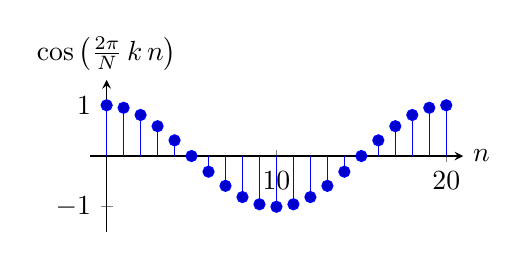
\begin{tikzpicture}
\begin{axis} [width=180pt,height=100pt,
	axis x line=middle, 
	axis y line=middle, 
	tick align=center,
	every axis x label/.style={at={(current axis.right of origin)},anchor=west},
	every axis y label/.style={at={(current axis.above origin)}, anchor=north east,above=0mm},
	xmin=-1, xmax=21,
	xtick={0,10,20},
	xlabel=$n$,
	ymin=-1.5, ymax=1.5,
	ytick={-1, 0,1},
	ylabel={$\cos\left(\frac{2 \pi}{N} \,k\,n \right)$},
	color=black]
 \addplot+[ycomb,domain=0:20,samples=21,samples y=0] 
 ({x}, {cos(deg(2*pi*x*1/20))}); 
\end{axis}
\end{tikzpicture}
}
%&
%\text{(b)}
\sublabel{b}{
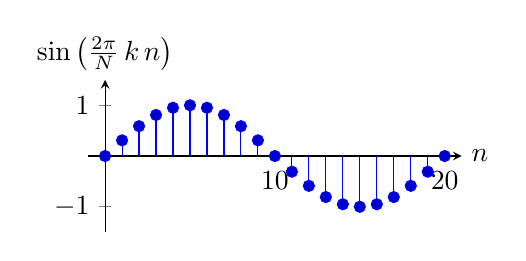
\begin{tikzpicture}
\begin{axis} [width=180pt,height=100pt,
	axis x line=middle, 
	axis y line=middle, 
	tick align=center,
	every axis x label/.style={at={(current axis.right of origin)},anchor=west},
	every axis y label/.style={at={(current axis.above origin)}, anchor=north east,above=0mm},
	xmin=-1, xmax=21,
	xtick={0,10,20},
	xlabel=$n$,
	ymin=-1.5, ymax=1.5,
	ytick={-1, 0,1},
	ylabel={$\sin\left(\frac{2 \pi}{N} \,k\,n \right)$}]
\addplot+[ycomb,domain=0:20,samples=21,samples y=0] 
 ({x}, {sin(deg(2*pi*x*1/20))}); 
\end{axis}
\end{tikzpicture}
}
%\end{array}
%\end{center}
}
\centerline{
%\[
%\begin{array}{cc}
\sublabel{c}{
%\text{(c)}
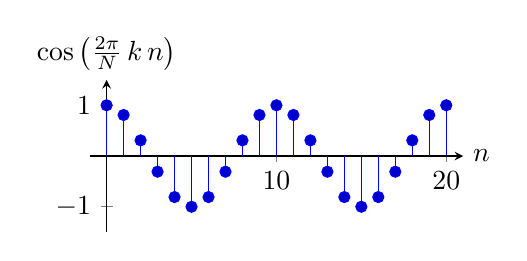
\begin{tikzpicture}
\begin{axis} [width=180pt,height=100pt,
	axis x line=middle, 
	axis y line=middle, 
	tick align=center,
	every axis x label/.style={at={(current axis.right of origin)},anchor=west},
	every axis y label/.style={at={(current axis.above origin)}, anchor=north east,above=0mm},
	xmin=-1, xmax=21,
	xtick={0,10,20},
	xlabel=$n$,
	ymin=-1.5, ymax=1.5,
	ytick={-1, 0,1},
	ylabel={$\cos\left(\frac{2 \pi}{N} \,k\,n \right)$},
	color=black]
 \addplot+[ycomb,domain=0:20,samples=21,samples y=0] 
 ({x}, {cos(deg(2*pi*x/10))}); 
\end{axis}
\end{tikzpicture}
}
%&
\sublabel{d}{
%\text{(d)}
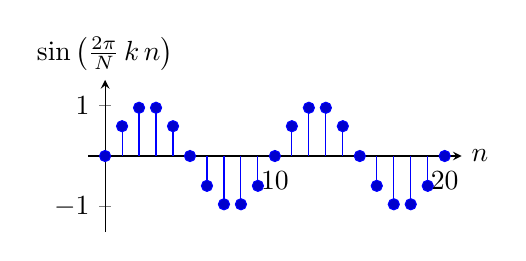
\begin{tikzpicture}
\begin{axis} [width=180pt,height=100pt,
	axis x line=middle, 
	axis y line=middle, 
	tick align=center,
	every axis x label/.style={at={(current axis.right of origin)},anchor=west},
	every axis y label/.style={at={(current axis.above origin)}, anchor=north east,above=0mm},
	xmin=-1, xmax=21,
	xtick={0,10,20},
	xlabel=$n$,
	ymin=-1.5, ymax=1.5,
	ytick={-1, 0,1},
	ylabel={$\sin\left(\frac{2 \pi}{N} \,k\,n \right)$}]
\addplot+[ycomb,domain=0:20,samples=21,samples y=0] 
 ({x}, {sin(deg(2*pi*x/10))}); 
\end{axis}
\end{tikzpicture}
}
%\end{array}
%\]
}
\centerline{
%\[
%\begin{array}{cc}
\sublabel{e}{
%\text{(e)}
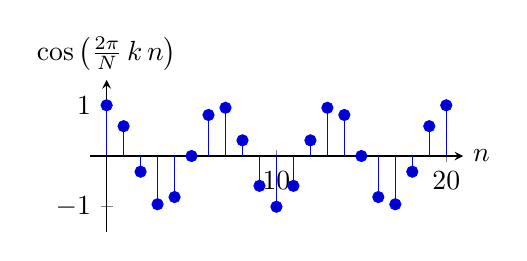
\begin{tikzpicture}
\begin{axis} [width=180pt,height=100pt,
	axis x line=middle, 
	axis y line=middle, 
	tick align=center,
	every axis x label/.style={at={(current axis.right of origin)},anchor=west},
	every axis y label/.style={at={(current axis.above origin)}, anchor=north east,above=0mm},
	xmin=-1, xmax=21,
	xtick={0,10,20},
	xlabel=$n$,
	ymin=-1.5, ymax=1.5,
	ytick={-1, 0,1},
	ylabel={$\cos\left(\frac{2 \pi}{N} \,k\,n \right)$},
	color=black]
 \addplot+[ycomb,domain=0:20,samples=21,samples y=0] 
 ({x}, {cos(deg(2*pi*x*3/20))}); 
\end{axis}
\end{tikzpicture}
}
%&
\sublabel{f}{
%\text{(f)}
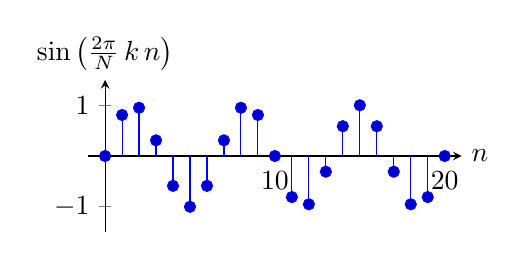
\begin{tikzpicture}
\begin{axis} [width=180pt,height=100pt,
	axis x line=middle, 
	axis y line=middle, 
	tick align=center,
	every axis x label/.style={at={(current axis.right of origin)},anchor=west},
	every axis y label/.style={at={(current axis.above origin)}, anchor=north east,above=0mm},
	xmin=-1, xmax=21,
	xtick={0,10,20},
	xlabel=$n$,
	ymin=-1.5, ymax=1.5,
	ytick={-1, 0,1},
	ylabel={$\sin\left(\frac{2 \pi}{N} \,k\,n \right)$}]
\addplot+[ycomb,domain=0:20,samples=21,samples y=0] 
 ({x}, {sin(deg(2*pi*x*3/20))}); 
\end{axis}
\end{tikzpicture}
}
%\end{array}
%\]
}
\caption{Sine and cosine waves with $A=1$ and $N=20$. Each row corresponds to $k=1$, $k=2$ and $k=3$. Note that for $k=3$ the waves oscillates three times in the interval $\left[0,N-1\right]$, but the samples in each oscillation are not identical, and it is only truly periodic once every $N$ samples. This is because $3/20$ is an irreducible fraction. }
\label{fig:contsignal}
\end{figure}

\begin{comment}

One remarkable property of sine and cosine waves is that the set of function $s_k$ and $c_k$ constitute what is called an orthogonal basis for all periodic discrete signals with period $N$, and also for all discrete signals of length $N$ (and a similar property exists also for continuous signals). Therefore, any such signal can be written as:
\begin{equation}
f\left[n\right] = a_0+ \sum_{k=1}^{N/2} a_k  \cos\left(\frac{2 \pi}{N} \,k\,n \right) + \sum_{k=1}^{N/2} b_k  \sin\left(\frac{2 \pi}{N} \,k\,n \right)
\end{equation}
were the coefficients $a_k$ and $b_k$ are constants. 
\begin{eqnarray}
\label{eq:fourier1}
a_0 &=& \frac{1}{N} \sum_{n=1}^{N-1}  \, f\left[n\right] \nonumber \\
a_k &=& \frac{2}{N} \sum_{n=1}^{N-1}   \, f\left[n\right] \cos\left(\frac{2 \pi}{N} \,k\,n \right) \nonumber \\
b_k &=& \frac{2}{N} \sum_{n=1}^{N-1}   \, f\left[n\right] \sin\left(\frac{2 \pi}{N} \,k\,n \right)
\end{eqnarray}
The set of coefficients ($a_k$, $b_k$) provide an alternative representation of the signal $f$ to the one provided by its sample values $f\left[n\right]$. As shown in equations \ref{eq:fourier1}, the coefficients ($a_k$, $b_k$) are a linear transformation of the samples $f\left[n\right]$.


The same analysis can be extended to 2 dimensions. In 2D, the discrete sine and cosine waves are:
\begin{equation}
s_{u,v}\left[n,m\right] = A \sin \left(2 \pi \left( \frac{u\,n}{N}  + \frac{v\,m}{M}  \right) \right)
\end{equation}
\begin{equation}
c_{u,v}\left[n,m\right] = A \cos \left(2 \pi \left( \frac{u\,n}{N}  + \frac{v\,m}{M}  \right) \right)
\end{equation}

\begin{figure}[h]
\begin{center}
\[
\begin{array}{ccc}
\text{a)}
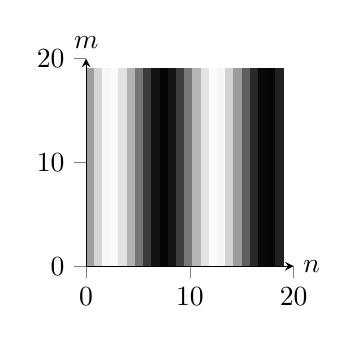
\begin{tikzpicture} 
\begin{axis}[width=120pt,height=120pt,
	mesh/ordering=y varies,
	view={0}{90},
	ymin=0, ymax=20,
	xmin=0, xmax=20,
	axis on top, 
	axis x line=bottom, 
	axis y line=left, 
	tick align=outside,
	every axis x label/.style={at={(current axis.right of origin)},anchor=west},
	every axis y label/.style={at={(current axis.north west)}, anchor=north west,above=0mm},
	xlabel={$n$}, ylabel={$m$}, zlabel={$z$}
	]  
\addplot3[surf,colormap/blackwhite,domain=0:19,shader=flat]  {sin(deg(2*pi*x*2/20 + 2*pi*y*0/20))};
\end{axis} 
\end{tikzpicture} 
&
\text{b)}
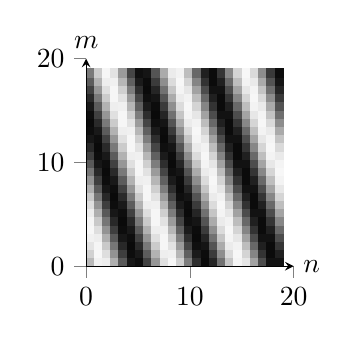
\begin{tikzpicture} 
\begin{axis}[width=120pt,height=120pt,
	mesh/ordering=y varies,
	view={0}{90},
	ymin=0, ymax=20,
	xmin=0, xmax=20,
	axis on top, 
	axis x line=bottom, 
	axis y line=left, 
	tick align=outside,
	every axis x label/.style={at={(current axis.right of origin)},anchor=west},
	every axis y label/.style={at={(current axis.north west)}, anchor=north west,above=0mm},
	xlabel={$n$}, ylabel={$m$}, zlabel={$z$}
	]  
\addplot3[surf,colormap/blackwhite,domain=0:19,shader=flat]  {sin(deg(2*pi*x*3/20 + 2*pi*y*1/20))};
\end{axis} 
\end{tikzpicture} 
&
\text{c)}
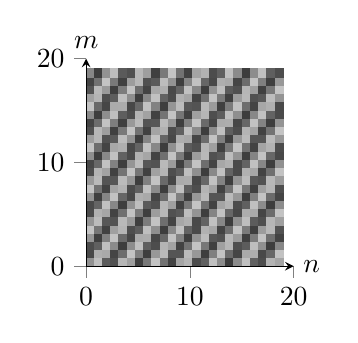
\begin{tikzpicture} 
\begin{axis}[width=120pt,height=120pt,
	mesh/ordering=y varies,
	view={0}{90},
	ymin=0, ymax=20,
	xmin=0, xmax=20,
	axis on top, 
	axis x line=bottom, 
	axis y line=left, 
	tick align=outside,
	every axis x label/.style={at={(current axis.right of origin)},anchor=west},
	every axis y label/.style={at={(current axis.north west)}, anchor=north west,above=0mm},
	xlabel={$n$}, ylabel={$m$}, zlabel={$z$}
	]  
\addplot3[surf,colormap/blackwhite,domain=0:19,shader=flat]  {sin(deg(2*pi*x*7/20 - 2*pi*y*5/20))};
\end{axis} 
\end{tikzpicture} 
\end{array}
\]
\end{center}
\caption{2D sine waves with $N=M=20$. The frequency values are: a) $u=2, v=0$, b) $u=3, v=1$, c) $u=7,v=-5$} 
\label{fig:disc2Dsignal}
\end{figure}


\end{comment}


\subsection{Sines and Cosines in 2D}

The same analysis can be extended to two dimensions (2D). In 2D, the discrete sine and cosine waves are as follows:

%Let's start by defining two very useful image families: the discrete sine and cosine waves. They are defined as:
 \begin{equation}
 s_{u,v}\left[n,m\right] = A \sin \left(2 \pi \left( \frac{u\,n}{N}  + \frac{v\,m}{M}  \right) \right)
 \end{equation}
 \begin{equation}
 c_{u,v}\left[n,m\right] = A \cos \left(2 \pi \left( \frac{u\,n}{N}  + \frac{v\,m}{M}  \right) \right)
 \end{equation}
 where $A$ is the amplitude and $u$ and $v$ are the two spatial frequencies and define how fast or slow the waves change along the spatial dimensions $n$ and $m$. \Fig{\ref{fig:disc2Dsignal}} shows some examples. 
 \begin{figure}[h]
 \centerline{
 %\[
 %$
 %\begin{array}{ccc}
 %\text{(a)}
\sublabel{a}{
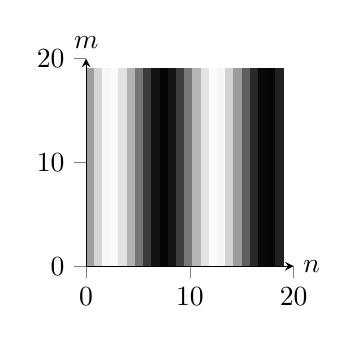
\begin{tikzpicture} 
 \begin{axis}[width=120pt,height=120pt,
 	mesh/ordering=y varies,
 	view={0}{90},
 	ymin=0, ymax=20,
 	xmin=0, xmax=20,
 	axis on top, 
 	axis x line=bottom, 
 	axis y line=left, 
 	tick align=outside,
 	every axis x label/.style={at={(current axis.right of origin)},anchor=west},
 	every axis y label/.style={at={(current axis.north west)}, anchor=north west,above=0mm},
 	xlabel={$n$}, ylabel={$m$}, zlabel={$z$}
 	]  
 \addplot3[surf,colormap/blackwhite,domain=0:19,shader=flat]  {sin(deg(2*pi*x*2/20 + 2*pi*y*0/20))};
 \end{axis} 
 \end{tikzpicture} 
 }
 %&
 %\text{(b)}
\sublabel{b}{
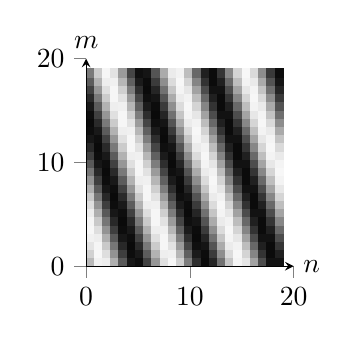
\begin{tikzpicture} 
 \begin{axis}[width=120pt,height=120pt,
 	mesh/ordering=y varies,
 	view={0}{90},
 	ymin=0, ymax=20,
 	xmin=0, xmax=20,
 	axis on top, 
 	axis x line=bottom, 
 	axis y line=left, 
 	tick align=outside,
 	every axis x label/.style={at={(current axis.right of origin)},anchor=west},
 	every axis y label/.style={at={(current axis.north west)}, anchor=north west,above=0mm},
 	xlabel={$n$}, ylabel={$m$}, zlabel={$z$}
 	]  
 \addplot3[surf,colormap/blackwhite,domain=0:19,shader=flat]  {sin(deg(2*pi*x*3/20 + 2*pi*y*1/20))};
 \end{axis} 
 \end{tikzpicture} 
 }
 %&
 %\text{(c)} 
\sublabel{c}{
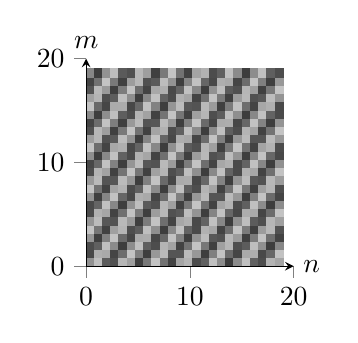
\begin{tikzpicture} 
 \begin{axis}[width=120pt,height=120pt,
 	mesh/ordering=y varies,
 	view={0}{90},
 	ymin=0, ymax=20,
 	xmin=0, xmax=20,
 	axis on top, 
 	axis x line=bottom, 
 	axis y line=left, 
 	tick align=outside,
 	every axis x label/.style={at={(current axis.right of origin)},anchor=west},
 	every axis y label/.style={at={(current axis.north west)}, anchor=north west,above=0mm},
 	xlabel={$n$}, ylabel={$m$}, zlabel={$z$}
 	]  
 \addplot3[surf,colormap/blackwhite,domain=0:19,shader=flat]  {sin(deg(2*pi*x*7/20 - 2*pi*y*5/20))};
 \end{axis} 
 \end{tikzpicture} 
 }
 %\end{array}
 %\]
 %$
 }
 \caption{2D sine waves with $N=M=20$. The frequency values are (a) $u=2, v=0$; (b) $u=3, v=1$; (c) $u=7,v=-5$.} 
 \label{fig:disc2Dsignal}
 \end{figure}

In 2D, the sine and cosine waves can also be described using polar coordinates for encoding the frequency: radial frequency, $\sqrt{u^2+v^2}$, and orientation, $\angle (u,v)$. 
\index{Radial frequency}
%In discrete time (setting $A=1$), we can write:
%\begin{equation}
%e_k\left[n\right] = \exp \left( j \frac{2 \pi}{N} \,k \,n \right) = \cos \left(\frac{2 \pi}{N} \,k \,n \right) + j \sin \left( \frac{2 \pi}{N} \,k \,n \right)
%\end{equation}







\subsection{Complex Exponentials}

Another important signal is the complex exponential wave: 
\begin{equation}
e_{u}\left[n\right] = \exp \left(2 \pi j   \frac{u\, n}{N}   \right) 
\end{equation}

Complex exponentials are related to cosine and sine waves by Euler's formula:
\index{Euler's formula}
\begin{equation}
\label{eq:euler}
\exp \left(j a\right) = \cos (a) + j \sin (a)
\end{equation}
\Fig{\ref{fig:complexexponential}} shows the one dimensional (1D) discrete complex exponential function (for $v=0$). As the values are complex, the plot shows in the $x$-axis the real component and in the $y$-axis the imaginary component. As $n$ goes from 0 to $N-1$ the function rotates along the complex circle of unit magnitude.


\begin{figure}[t]
\centerline{
%\[
%$
%\begin{array}{cc}
%\text{(a)}
\sublabel{a}{
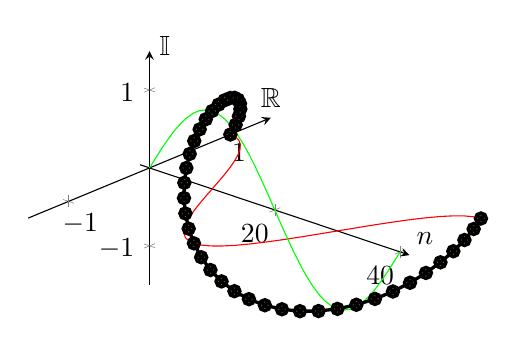
\begin{tikzpicture} 
\begin{axis}[view={42}{30}, width=230pt,
	axis x line=middle, 
	axis y line=middle, 
	axis z line=middle, 
	tick align=center,
	ymin=-1.5, ymax=1.5,
	zmin=-1.5, zmax=1.5,
	xmin=-1.5, xmax=41.5,
	%,anchor=near ticklabel
	%every axis z label/.style={at={(0,0,1)},left=0mm,above=0mm},
	%every axis x label/.style={at={(current axis.right of origin)},anchor=west,left=16mm,above=2mm},
	%every axis y label/.style={at={(current axis.above origin)},anchor=north east,above=-8mm,left=57mm},
        xlabel=$n$,ylabel=$\mathbb{R}$,zlabel=$\mathbb{I}$,
        %y dir=reverse,
        every axis y label/.append style={at=(ticklabel* cs:1.0),above=0mm},
        every axis x label/.append style={at=(ticklabel* cs:1.1)},
        every axis z label/.append style={at=(ticklabel* cs:1.1)}
]
 \addplot3[domain=0:40,samples=41,samples y=0,draw=red] 
 ({x}, {cos(deg(2*pi*1*x/40))}, {0}); 
\addplot3[domain=0:40,samples=41,samples y=0,draw=green] 
 ({x}, {0}, {sin(deg(2*pi*1*x/40))}); 
 \addplot3+[domain=0:40,samples=41,samples y=0,very thick,draw=black] 
 %({cos(deg(x))}, {x}, {sin(deg(x))}); 
 ({x}, {cos(deg(2*pi*1*x/40))}, {sin(deg(2*pi*1*x/40))}); 
 \end{axis} 
 \end{tikzpicture}
 }
 %&
%\text{(b)}
\sublabel{b}{
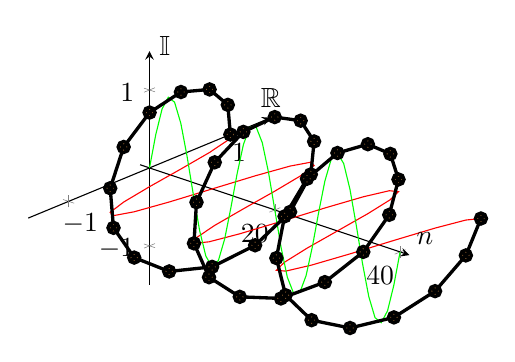
\begin{tikzpicture} 
\begin{axis}[view={42}{30}, width=230pt,
	axis x line=middle, 
	axis y line=middle, 
	axis z line=middle, 
	tick align=center,
	ymin=-1.5, ymax=1.5,
	zmin=-1.5, zmax=1.5,
	xmin=-1.5, xmax=41.5,
	%,anchor=near ticklabel
	%every axis z label/.style={at={(0,0,1)},left=0mm,above=0mm},
	%every axis x label/.style={at={(current axis.right of origin)},anchor=west,left=16mm,above=2mm},
	%every axis y label/.style={at={(current axis.above origin)},anchor=north east,above=-8mm,left=57mm},
        xlabel=$n$,ylabel=$\mathbb{R}$,zlabel=$\mathbb{I}$,
        %y dir=reverse,
        every axis y label/.append style={at=(ticklabel* cs:1.0),above=0mm},
        every axis x label/.append style={at=(ticklabel* cs:1.1)},
        every axis z label/.append style={at=(ticklabel* cs:1.1)}
]
 \addplot3[domain=0:40,samples=41,samples y=0,draw=red] 
 ({x}, {cos(deg(2*pi*3*x/40))}, {0}); 
\addplot3[domain=0:40,samples=41,samples y=0,draw=green] 
 ({x}, {0}, {sin(deg(2*pi*3*x/40))}); 
 \addplot3+[domain=0:40,samples=41,samples y=0,very thick,draw=black] 
 %({cos(deg(x))}, {x}, {sin(deg(x))}); 
 ({x}, {cos(deg(2*pi*3*x/40))}, {sin(deg(2*pi*3*x/40))}); 
 \end{axis} 
 \end{tikzpicture}
 }
%\end{array}
%\]
%$
}
%\vspace{-0.5in}
\caption{Complex exponential wave with (a) $N=40$, $k=1$, $A=1$; and (b) $N=40$, $k=3$, $A=1$. The red and green curves show the real and imaginary waves. The black line is the complex exponential. The dots correspond to the discrete samples.} 
\label{fig:complexexponential}
\end{figure}


In 2D, the complex exponential wave is
\begin{equation}
e_{u,v}\left[n,m\right] = \exp \left(2 \pi j \left(  \frac{u\, n}{N}  + \frac{v\,m}{M}  \right) \right) 
\end{equation}
where $u$ and $v$ are the two spatial frequencies. Note that complex exponentials in 2D are separable. This means they can be written as the product of two 1D signals:
\begin{equation}
e_{u,v}\left[n,m\right]   = e_{u}\left[n\right] e_{v}\left[m\right] 
\end{equation}

 

%
%The set of functions $e_k\left[n\right]$, with $k\in\left[0,N-1\right]$, form an orthogonal basis for discrete signals of length $N$. In fact, 
%\begin{equation}
%\left<e_k, e_r \right> = \sum_{n=0}^{N-1} e_k\left[n\right] e^*_r\left[n\right] = N \delta \left[k-r\right] = 
% \begin{cases}
%    N       & \quad \text{if } k=r\\
%    0       & \quad \text{if } k \neq r\\
%  \end{cases}
%\end{equation}

A remarkable property is that the complex exponentials form an orthogonal basis for discrete signals and images of finite length. For images of size $N \times M$,
\begin{equation}
\left<e_{u,v}, e_{u',v'} \right> = \sum_{n=0}^{N-1} \sum_{m=0}^{M-1} e_{u,v}\left[n,m\right] e^*_{u',v'}\left[n,m\right] = MN \delta \left[u-u'\right]\delta \left[v-v'\right] 
\end{equation}
Therefore, any finite length discrete image can be decomposed as a linear combination of complex exponentials. 


%\begin{eqnarray}
%\label{eq:euler}
%\cos{ \left( 2\pi \left( \frac{u\, n}{N} + \frac{v m}{M} \right) \right) } &=& \frac{1}{2} \left( e_{u,v}\left[n,m\right]  +  e^*_{u,v}\left[n,m\right]  \right) \\
%\sin{ \left( 2\pi \left( \frac{u\, n}{N} + \frac{v m}{M} \right) \right) } &=& \frac{-j}{2} \left( e_{u,v}\left[n,m\right]  - e^*_{u,v}\left[n,m\right]  \right)
%\end{eqnarray}
%
%


\section{The Discrete Fourier Transform}

In this chapter we will focus on the discrete Fourier transform as it provides important tools to understand the behavior of signals and systems (e.g., sampling and convolutions). For a more detailed study of other transforms and the foundations of Fourier series we refer the reader to other specialized books in signal and image processing .

\subsection{Discrete Fourier Transform and Inverse Transform}

The {\bf Discrete Fourier Transform} (DFT) transforms an image $\img \left[n,m \right]$, of finite size $N \times M$, into the complex image Fourier transform $\capitalimg \left[u,v \right]$ as:
\begin{equation}
\capitalimg \left[u,v \right] =  
\mathcal{F} \left\{ \img \left[n,m \right] \right\}
=
\sum_{n=0}^{N-1} \sum_{m=0}^{M-1} \, \img \left[n,m \right] 
\exp{ \left( -2\pi j \left( \frac{u\, n}{N} + \frac{v\, m}{M} \right) \right)}
\label{eq:fourier}
\end{equation}
We will call $\capitalimg \left[u,v \right]$ the Fourier transform of $\img \left[m,n \right]$. We will often represent the relationship between the signal as its transform as:
\begin{equation}
\img \left[n,m \right] \xrightarrow{\mathscr{F}} \capitalimg \left[u,v \right]
\end{equation}


By applying 
$\frac{1}{MN} \sum_{u=0}^{M-1} \sum_{v=0}^{N-1}$
to both sides of \eqn{\ref{eq:fourier}} and exploiting the orthogonality between distinct Fourier basis elements, we find the {\bf inverse Fourier transform} relation
\begin{equation}
\img \left[n,m \right] = 
\mathcal{F}^{-1} \left\{ \capitalimg \left[u,v \right] \right\}
=
\frac{1}{NM} \sum_{u=0}^{N-1} \sum_{v=0}^{M-1} \capitalimg \left[u,v \right] 
\exp{ \left(+2\pi j \left(\frac{u\, n}{N} + \frac{v\, m}{M} \right) \right) }
\label{eq:inversefourier}
\end{equation}


As we can see from the inverse transform equation, we rewrite the image, instead of as a sum of offset pixel
values, as a sum of complex exponentials, each at a different frequency, called a spatial frequency for images because they describe
how quickly things vary across space.  From the inverse transform formula, we see that to construct an image
from a Fourier transform, $\capitalimg \left[u,v \right]$, we just add in the corresponding
amount of that particular complex exponential (conjugated).

As $\capitalimg \left[u,v \right]$ is obtained as a sum of complex exponential with a common period of $N,M$ samples, the function  $\capitalimg \left[u,v \right]$  is also periodic: $\capitalimg \left[u+aN,v+bM \right] = \capitalimg \left[u,v \right]$ for any $a,b \in \mathbb{Z}$.
Also the result of the inverse DFT is a periodic image. Indeed you can verify from \eqn{\ref{eq:inversefourier}} that $\img \left[n+aN,m+bM \right] = \img \left[n,m \right]$ for any $a,b \in \mathbb{Z}$. 


% Source: https://en.wikipedia.org/wiki/Cooley%E2%80%93Tukey_FFT_algorithm

Using the fact that $e_{N-u, M-v} = e_{-u,-v}$, another equivalent way to write for the Fourier transform is to sum over the frequency interval $\left[-N/2, N/2\right]$ and $\left[-M/2, M/2\right]$. This is especially useful for the inverse that can be written as:
\begin{equation}
\img \left[n,m \right] = \frac{1}{NM} \sum_{u=-N/2}^{N/2} \sum_{v=-M/2}^{M/2} \capitalimg \left[u,v \right] 
\exp{ \left(+2\pi j \left(\frac{u\, n}{N} + \frac{v\, m}{M} \right) \right) }
\label{eq:inversefourier2}
\end{equation}

This formulation allows us to arrange the coefficients in the complex plane so that the zero frequency, or DC, coefficient is at the center.  Slow, large variations correspond to complex exponentials of
frequencies near the origin.   If the amplitudes of the complex conjugate exponentials are the same, then their sum will represent a cosine wave;  if their amplitudes are opposite, it will be a sine
wave.  Frequencies further away from the origin represent faster
variation with movement across space. The DFT and its inverse in 1D are defined in the same way as shown in table \ref{table:tableFamilyFT}. 


One very important property is that the decomposition of a signal into a sum of complex exponentials is unique: there is a unique linear combination of the exponentials that will result in a given signal. 

\marginnote{The DFT became very popular thanks to the {\bf Fast Fourier Transform} (FFT) algorithm. The most common FFT algorithm is the Cooley–Tukey algorithm \cite{Cooley1965} that reduces the computation cost from $O(N^2)$ to $O(N \log N)$.}[-1.1in]
\index{Fast Fourier transform}

\subsection{Matrix Form of the Fourier Transform}



As the DFT is a linear transform we can also write the DFT in matrix form, with one basis per row. In 1D, the matrix for the DFT is as follows:

\begin{equation}
    \mathbf{F} = \begin{bmatrix}
1 & 1 & 1 & \dots & 1\\ %u=0
1 & \exp{ \left(-2\pi j \frac{1}{N} \right)} & \exp{ \left(-2\pi j \frac{2}{N} \right)} & \dots & \exp{ \left(-2\pi j \frac{N-1}{N} \right)}\\ %u=1
1 & \exp{ \left(-2\pi j \frac{2}{N} \right)} & \exp{ \left(-2\pi j \frac{4}{N} \right)} & \dots & \exp{ \left(-2\pi j \frac{2\, (N-1)}{N} \right)}\\ %u=2
\vdots & \vdots & \vdots & ~ & \vdots \\
1 & \exp{ \left(-2\pi j \frac{(N-1)}{N} \right)} & \exp{ \left(-2\pi j \frac{(N-1)\, 2}{N} \right)} & \dots & \exp{ \left(-2\pi j \frac{(N-1)\, (N-1)}{N} \right)}\
\end{bmatrix}
\end{equation}
Each entry in the matrix is $\mathbf{F}_{u,n} = \exp{ \left(-2\pi j \frac{u\, n}{N} \right)}$, with $u$ indexing rows and $n$ indexing columns. Note that $\mathbf{F}$ is a symmetric matrix. The inverse of the DFT is the complex conjugate: $\mathbf{F}^{-1} = \mathbf{F}^{*}$.

Working in 1D, as we did before, allows us to visualize the transformation matrix. \Fig{\ref{fig:colorDFT}} shows a color visualization of the
complex-value matrix for the 1D DFT, which when used as a multiplicand yields the Fourier transform of 1D vectors.  Many Fourier transform properties and symmetries can be observed from inspecting that matrix. %Note that this matrix also has some similarities with the matrix used to compute the 1D DCT.


\begin{figure}[t]
\centerline{
\includegraphics[width=0.7\linewidth]{figures/Image_processing_fourier/visualization_DFT_color.eps}}
\caption{Visualization of the discrete Fourier transform as a matrix.  The signal to be
 transformed forms the entries of the column vector at right.  The
 complex values of the Fourier transform matrix are indicated by the color,
 with the key in the bottom left.  In the vector at the right, black
 values indicate zero.
} 
\label{fig:colorDFT}
\end{figure}

\subsection{Visualizing the Fourier Transform}


When computing the DFT of a real image, we will not be able to write the analytic form of the result, but there are a number of properties that will help us to interpret the result. \Fig{\ref{fig:DFT_a}} shows the Fourier transform of a $64 \times 64$ resolution image of a cube.
As the DFT results in a complex representation, there are two possible ways of writing the result. Using the real and imaginary components:
\begin{equation}
\capitalimg \left[u,v \right] = Re \left\{\capitalimg \left[u,v \right] \right\}  + j \, Imag \left\{\capitalimg \left[u,v \right] \right\}
\end{equation}
where $Re$ and $Imag$ denote the real and imaginary part of each Fourier coefficient. Or using a polar decomposition:
\begin{equation}
\capitalimg \left[u,v \right]  = A \left[u,v \right] \, \exp{\left( j \, \theta\left[u,v \right]  \right)}
\end{equation}
where $A \left[u,v \right] \in \mathbb{R}^+$ is the amplitude and $\theta \left[u,v \right] \in \left[-\pi, \pi \right]$ is the phase. 
\Fig{\ref{fig:DFT_a}} shows both decompositions of the Fourier transform.


\begin{figure}[t]
\centerline{
\includegraphics[width=1\linewidth]{figures/Image_processing_fourier/dft_a.eps}
}
\caption{DFT of an image and visualization of (top) the real and imaginary components,
and (bottom) the amplitude and phase  of the Fourier transform.} 
\label{fig:DFT_a}
\end{figure}

Upon first learning about Fourier transforms, it may be a surprise for readers to learn that one can synthesize any image as a sum of complex exponentials (i.e., sines and cosines).  To help gain insight into how that works, it is informative to show examples of partial sums of complex exponentials. \Fig{\ref{fig:DFT_b}} shows partial sums of the Fourier components
of an image.  In each partial sum of $N$ components, we use the largest N components of the Fourier transform.
Using the fact that the Fourier basis functions are orthonormal, it is straightforward to show that this is the best least-squares reconstruction possible from each given number of Fourier basis
components.  This first image shows what is reconstructed from the largest Fourier component which turns out to be $\capitalimg \left[0,0 \right]$. This component encodes the DC value of the image, therefore the resulting image is just a constant. The next two components correspond to two complex conjugates of a very slow varying wave. And so on. As more components get added, the figure slowly emerges. In this example, the first 127 coefficients are sufficient for recognizing this 64$\times$64 resolution image.


\begin{figure}[t]
\centerline{
\includegraphics[width=1\linewidth]{figures/Image_processing_fourier/dft_b.eps}
}
\caption{Reconstructing an image from the $N$ Fourier coefficients of
  the largest amplitude.  The right frame shows the location, in the
  Fourier domain, of the $N$ Fourier coefficients, which when
  inverted, give the image at the left.
} 
\label{fig:DFT_b}
\end{figure}

\section{Useful Transforms}

It's useful to become adept at computing and manipulating
simple Fourier transforms.  For some simple cases, we can compute the analytic form of the Fourier transform.

\subsection{Delta Distribution}

The Fourier transform of the delta function $\delta \left[n,m \right]$ is
\begin{equation}
\mathcal{F} \left\{ \delta \left[n,m \right] \right\} = 
%X \left[u,v \right] =  
\sum_{n=0}^{N-1} \sum_{m=0}^{M-1} \, \delta \left[n,m \right] 
\exp{ \left( -2\pi j \left( \frac{u\, n}{N} + \frac{v\, m}{M} \right) \right)} = 1
\end{equation}
where the Fourier transform of the delta signal is 1. 
\begin{equation}
\delta \left[n,m \right] \xrightarrow{\mathscr{F}} 1
\end{equation}
If we think in terms of the inverse Fourier transform, this means that if we sum all the complex exponentials with a coefficient of 1, then all the values will cancel but the one at the origin, which results in a delta function:
\begin{equation}
\delta \left[n,m \right] = \frac{1}{NM} \sum_{u=-N/2}^{N/2} \sum_{v=-M/2}^{M/2}  
\exp{ \left(2\pi j \left(\frac{u\, n}{N} + \frac{v\, m}{M} \right) \right) }
\end{equation}

\subsection{Cosine and Sine Waves}

The Fourier transform of the cosine wave, $\cos{ \left( 2\pi \left( \frac{u_0\, n}{N} + \frac{v_0\, m}{M} \right) \right) }$, is:
\begin{eqnarray}
\sum_{n=0}^{N-1} \sum_{m=0}^{M-1} \, \cos{ \left( 2\pi \left( \frac{u_0 \, n}{N} + \frac{v_0 \, m}{M} \right) \right) }
\exp{ \left( -2\pi j \left( \frac{u\, n}{N} + \frac{v\, m}{M} \right) \right)} = \\ 
=\frac{1}{2} \left( \delta \left[u-u_0, v-v_0 \right] +  \delta \left[u+u_0, v+v_0 \right] \right)
\end{eqnarray}
This can be easily proven using Euler's \eqn{\ref{eq:euler}} and the orthogonality between complex exponentials. This results in the Fourier transform relationship: 
\begin{equation}
\cos{ \left( 2\pi \left( \frac{u_0\, n}{N} + \frac{v_0\, m}{M} \right) \right) } 
\xrightarrow{\mathscr{F}} 
\frac{1}{2} \left( \delta \left[u-u_0, v-v_0 \right] +  \delta \left[u+u_0, v+v_0 \right] \right)
\end{equation}

And for the sine wave, $\sin{ \left( 2\pi \left( \frac{u_0\, n}{N} + \frac{v_0 m}{M} \right) \right) }$, we have a  similar relationship:


\begin{equation}
\sin{ \left( 2\pi \left( \frac{u_0\, n}{N} + \frac{v_0 m}{M} \right) \right) } 
\xrightarrow{\mathscr{F}} 
\frac{1}{2j} \left( \delta \left[u-u_0, v-v_0 \right] - \delta \left[u+u_0, v+v_0 \right]\right)
\end{equation}

\Fig{\ref{fig:2ddftexampleswaves}} shows the DFT of several waves with different frequencies and orientations. 


\begin{figure}[t]
\centerline{
\includegraphics[width=1\linewidth]{figures/Image_processing_fourier/DFT_examples_waves.eps}
}
\caption{Some 2D Fourier transform pairs. Images are $64 \times 64$ pixels. The waves are cosine with frequencies $(1,2)$, $(5,0)$, $(10,7)$, $(11,-15)$. The last two examples show the sum of two waves and the product.  
} 
\label{fig:2ddftexampleswaves}
\end{figure}


\Fig{\ref{fig:2ddftexamples}} shows the 2D Fourier transforms of
some periodic signals.  The depicted signals all happen to be symmetric
about the spatial origin.  From the Fourier transform equation, one
can show that real and even input signals transform to real and even
outputs.  So for the examples of \fig{\ref{fig:2ddftexamples}}, we only
show the magnitude of the Fourier transform, which in this case is the
absolute value of the real component of the transform, and the
imaginary component happens to be zero for the signals we'll examine. Also, all these images but the last one are separable (they can be written as the product of two 1D signals). Therefore, their DFT is also the product of 1D DFTs.


\begin{figure}
\centerline{
\includegraphics[width=1\linewidth]{figures/Image_processing_fourier/DFT_toy_examples.eps}
}
\caption{Some two-dimensional Fourier transform pairs.
  Note the trends visible in the collection of transform pairs:  As
  the support of the image in one domain gets larger, the magnitude in
  the other domain becomes more localized.  A line transforms to a
  line oriented perpendicularly to the first. Images are $64 \times 64$ pixels, origin is in the center.
} 
\label{fig:2ddftexamples}
\end{figure}

\subsection{Box Function}
\label{sec:box_function}
The box function is a very useful function that we will use several times in this book. It is good to be familiar with its Fourier transform and how to compute it. The box function is defined as follows:
\begin{equation}
\text{box}_{L} \left[n \right] = 
\begin{cases}
    1       & \quad \text{if } -L \leq n \leq L  \\
    0       & \quad \text{otherwise.} 
  \end{cases}
\end{equation}

The box function takes values of 1 inside the interval $\left[ -L,L \right]$ and it is 0 outside. The duration of the box is $2L+1$.

It is useful to think of the box function as a finite length signal of length $N$ and to visualize its periodic extension outside of that interval. The following plot shows the box function for $L=5$ and $N=32$. In this plot, the box signal is defined between $-N/2=-16$ and $N/2-1=15$ and the rest is its periodic extension. 

\begin{figure}[h]
\centerline{
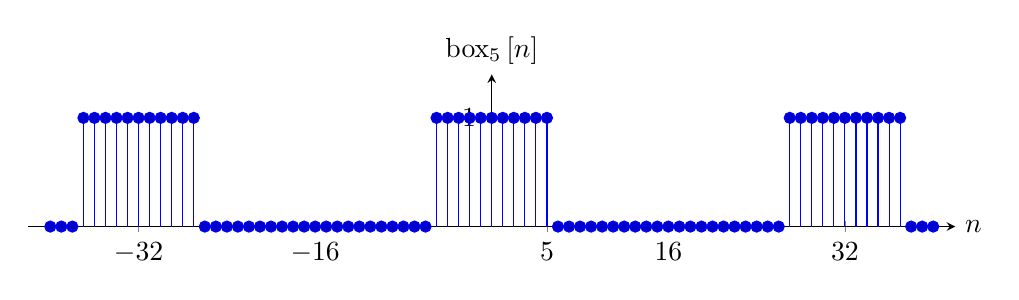
\begin{tikzpicture}
\begin{axis} [width=380,height=100pt,
	axis x line=bottom, 
	axis y line=middle, 
	tick align=center,
	every axis x label/.style={at={(current axis.right of origin)},anchor=west},
	every axis y label/.style={at={(current axis.above origin)}, anchor=north east,above=0mm},
	xmin=-42, xmax=42,
	xtick={-32,-16, -5 0, 5, 16,32},
	xlabel=$n$,
	ymin=0, ymax=1.4,
	ytick={0,...,1},
	ylabel={$\text{box}_{5} \left[n \right]$}]
 \addplot+[ycomb,domain=-40:40,samples=81,samples y=0] 
 ({x}, {(abs(mod(x,32))<6)+(abs(mod(x,32))>26)}); 
 \end{axis} 
\end{tikzpicture}
}
\caption{Box function for $L=5$ and $N=32$.}
\end{figure}

We will compute here the DFT of the finite length box function, with a length $N$. To compute the DFT we use the DFT definition and change the interval of the sum making use of the periodic nature of the terms inside the sum:
\begin{eqnarray}
\mathcal{F} \left\{ \text{box}_{L} \left[n \right] \right\} &=& 
\sum_{n=0}^{N-1} \, \text{box}_{L} \left[n \right] 
\exp{ \left( -2\pi j \frac{u\, n}{N} \right)} \\
&=& \sum_{n=-L}^{L} \,
\exp{ \left( -2\pi j \frac{u\, n}{N} \right)} 
\label{eq:boxdftderivation}
\end{eqnarray}

We can use the equation of the sum of a geometric series:
\begin{equation}
\sum_{n=-L}^{L} a^n = a^{-L} \sum_{n=0}^{2L} a^n = a^{-L} \frac{1-a^{2L+1}}{1-a} = \frac{a^{-(2L+1)/2}-a^{(2L+1)/2}}{a^{-1/2}-a^{1/2}}
\end{equation}
where $a$ is a constant. With $a = \exp{ \left( -2\pi j \frac{u}{N} \right)}$ we can write the sum in \eqn{\ref{eq:boxdftderivation}} as

\begin{eqnarray}
\sum_{n=-L}^{L} \,
\exp{ \left( -2\pi j \frac{u\, n}{N} \right)} & = & 
\frac{\exp{ \left( \pi j \frac{u(2L+1)}{N} \right)} - \exp{ \left( -\pi j \frac{u(2L+1)}{N} \right)}}
{\exp{ \left( \pi j \frac{u}{N} \right)} - \exp{ \left( - \pi j \frac{u}{N} \right)} } \\
& = & \frac{\sin \left( \pi u(2L+1)/N \right)}{\sin \left( \pi u/N \right)}
\label{eq:discrete_sinc_function}
\end{eqnarray}

This last function in \eqn{\ref{eq:discrete_sinc_function}} gets the special name of {\bf discrete sinc} function. 
\marginnote{
The discrete sinc function ({\bf sincd}) is defined as follows:
\begin{equation*}
\text{sincd}(x;a) = \frac{\sin(\pi x)}{a \sin (\pi x/a)}
\end{equation*}
Where $a$ is a constant. This is a symmetrical periodic function with a maximum value of 1.
}[-.6in]

In summary, we get that The DFT of the box function is the discrete sinc function: 
\begin{equation}
\text{box}_{L} \left[n \right] 
\xrightarrow{\mathscr{F}} 
\frac{\sin \pi u (2L+1)/N}{\sin \pi u/N} 
\end{equation}
We will denote the DFT of the box function, $\text{box}_{L} \left[n \right]$, capitalizing the first letter, $\text{Box}_{L} \left[u \right]$.
This function has its maximum value at $u=0$. The DFT, $\text{Box}_{L} \left[u \right]$, is a symmetric real function.
The following plot (\fig{\ref{fig:boxfilterdft}}) shows the DFT of the box with $L=5$, and $N=32$. One period of the DFT is contained in the interval $\left[ -16, 15 \right]$ and the rest is a periodic extension.

\begin{figure}[h]
\centerline{
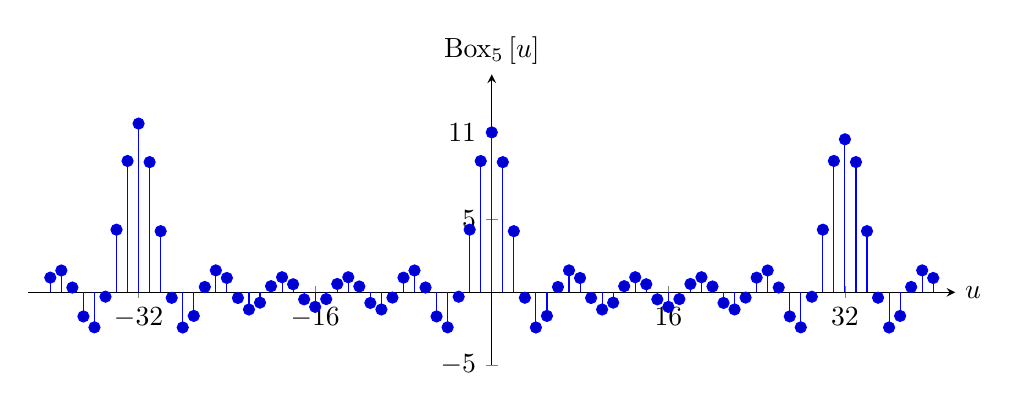
\begin{tikzpicture}
\begin{axis} [width=380pt,height=150pt,
	axis x line=middle, 
	axis y line=middle, 
	tick align=center,
	every axis x label/.style={at={(current axis.right of origin)},anchor=west},
	every axis y label/.style={at={(current axis.above origin)}, anchor=north east,above=0mm},
	xmin=-42, xmax=42,
	xtick={-32, -16, 0, 16, 32},
	xlabel=$u$,
	ymin=-5, ymax=15,
	ytick={-5,0,5,11},
	ylabel={$\text{Box}_{5} \left[u \right]$},
	color=black]
 \addplot+[ycomb,domain=-40:40,samples=81,samples y=0] 
 ({x}, {sin(deg(pi*(x+0.01)*(11)/32))) / sin(deg(pi*(x+0.01)/32)))}); 
\end{axis}
\end{tikzpicture}
}
\caption{DFT of the box filter with $L=5$, and $N=32$}
\label{fig:boxfilterdft}
\end{figure}

Now that we know how to compute the DFT of the 1D box, we can easily extend it to the 2D case. A 2D box is a separable function and can be written as the product of two box functions,
$\text{box}_{L_n, L_m} \left[n,m\right] = \text{box}_{L_n} \left[n\right] \text{box}_{L_m}\left[m\right]$. The DFT is the product of the two DFTs, 
\begin{equation}
\text{Box}_{L_n, L_m} \left[ u,v \right] = \text{Box}_{L_n} \left[ u\right] \text{Box}_{L_m} \left[ v\right].
\end{equation}

\Fig{\ref{fig:2ddftexamples}} shows several DFTs of 2D boxes of different sizes and aspect ratios.

\section{Discrete Fourier Transform Properties}
\label{section:DFTproperties}

It is important to be familiar with the properties for the DFT. Table \ref{table:tableDFT} summarizes some important transforms and properties. 


%For now, when we talk about images or signals we will assume they are periodic signals with periods $N$ and $M$ in each dimension. 


\begin{table}[t]
%\marginnote{{\bf Table \ref{table:tableDFT}}: Table of basic DFT transforms and properties.} % Hack to get the caption of the table in the margin.
%\faketablecaption{} % this updates the counter without plotting a caption.
\caption{Table of basic DFT transforms and properties.} % Hack to get the caption of the table in the margin.
%\caption{Table of basic DFT transforms and properties}
\begin{center}
\begin{tabular}{| c | c |}
\hline
\bf $\img \left[ n \right]$ & \bf $\capitalimg \left[u \right]$ \\
\hline \hline
$\img_1 \left[ n \right] \circ \img_2 \left[ n \right]$& $\capitalimg_1 \left[u \right] \capitalimg_2 \left[u \right]$ \\
\hline
$\img_1 \left[ n \right]$ $\img_2 \left[ n \right]$& $\frac{1}{N} \capitalimg_1 \left[u \right] \circ \capitalimg_2 \left[u \right]$ \\
\hline
$\img \left[ n-n_0 \right]$ & $\capitalimg \left[u \right] \exp{ \left( - 2 \pi j \frac{u n_0}{N} \right) }$  \\
\hline
$\delta \left[ n \right]$ & $1$ \\
\hline
$\exp{ \left( 2 \pi u_0 \frac{n}{N} \right) }$ &
$\delta \left[u-u_0 \right]$ \\
\hline
$\cos{ \left( 2 \pi u_0 \frac{n}{N} \right) }$ &
$\frac{1}{2} \left( \delta \left[u-u_0 \right] +  \delta \left[u+u_0\right] \right)$ \\
\hline
$\sin{ \left( 2 \pi u_0 \frac{n}{N} \right) }$ &
$\frac{1}{2j} \left( \delta \left[u-u_0 \right] -  \delta \left[u+u_0\right] \right)$ \\
\hline
$\text{box}_{L} \left[n \right]$ & $\frac{\sin \pi u (2L+1)/N}{\sin \pi u/N}$ \\
\hline
\end{tabular}
\end{center}
\label{table:tableDFT}
\end{table}

\subsection{Linearity}

The Fourier transform and its inverse are linear transformations:
%\begin{equation}
%DFT \left\{\alpha f\left[n,m \right] + \beta g\left[n,m \right] \right\} = \alpha F\left[u,v \right] +\beta G\left[u,v \right] 
%\end{equation}
\begin{equation}
\alpha \img_1 \left[n,m \right] + \beta \img_2 \left[ n,m \right]  
\xrightarrow{\mathscr{F}} 
\alpha \capitalimg_1 \left[u,v \right] + \beta \capitalimg_2 \left[ u,v \right]
\end{equation}
where $\alpha$ and $\beta$ are complex numbers. This property can be easily proven from the definition of the DFT. \Fig{\ref{fig:colorDFT}} shows a color visualization of the complex-value matrix for the 1D DFT.

\subsection{Separability}

An image is separable if it can be written as the product of two 1D signals, $\img \left[n,m \right] = \img_1\left[n \right] \img_2\left[m \right]$. If an image is separable, then its Fourier transform is separable:
%\begin{equation}
%DFT \left\{ f\left[n,m \right] \right\} = DFT \left\{ f_1\left[n \right] \right\} DFT \left\{ f_2\left[m \right] \right\}
%\end{equation}
%
%\begin{equation}
$\capitalimg \left[u,v \right] = \capitalimg_1 \left[u \right] \capitalimg_2 \left[v \right]$
%\end{equation}

\marginnote{{\bf Separability}. Although almost all images are not separable, some can be approximated by a separable image. Here is one example.
We can use the SVD decomposition to find a separable approximation to the image on the left. The result is shown on the right. 
\\[6pt]
\centerline{
\includegraphics[width=.4\linewidth]{figures/Image_processing_fourier/facade1.jpg}
~~~~~~~~
\includegraphics[width=.4\linewidth]{figures/Image_processing_fourier/facade1aprox.jpg}
}
The right-hand image can be written as the product of two 1D signals.
}[-7.7cm]



\subsection{Parseval's Theorem}

As the DFT is a change of basis, the dot product between two signals and the norm of a vector is preserved (up to a constant factor) after the basis change. This is stated by Parseval's theorem:
\begin{equation}
\sum_{n=0}^{N-1} \sum_{m=0}^{M-1} \,  \img_1 \left[n,m \right] \img_2^* \left[n,m \right] = \frac{1}{NM}\sum_{u=0}^{N-1} \sum_{v=0}^{M-1} \,  \capitalimg_1 \left[u,v \right] \capitalimg_2^* \left[u,v \right]
\end{equation}
In particular, if $\img_1=\img_2$ this reduces to the {\bf Plancherel theorem}:
\begin{equation}
\sum_{n=0}^{N-1} \sum_{m=0}^{M-1} \,  \| \img \left[n,m \right] \|^2 = \frac{1}{NM}\sum_{u=0}^{N-1} \sum_{v=0}^{M-1} \,  \| \capitalimg \left[u,v \right] \|^2
\end{equation}
This relationship is important because it tells us that the energy of a signal can be computed as the sum of the squared magnitude of the values of its Fourier transform. 

\subsection{Convolution}

Consider a signal $\imgout$ that is the result of applying (circular) convolution
of two signals, $\img_1$ and $\img_2$, both of size $N \times M$:
\begin{equation} 
\imgout = \img_1 \circ \img_2
\end{equation} 

The question is; how does the Fourier transform of the signal $\imgout$ relates to the Fourier transforms of the two signals $\img_1$ and $\img_2$?

\marginnote{The relationship between the convolution and the Fourier transform is probably the most important property of the Fourier transform and you should be familiar with it.}


If we take the Fourier transform of both sides, and use the
definition of the Fourier transform, we obtain
\begin{equation}
\begin{split}
\capitalimgout \left[u,v \right] & =  \mathcal{F}  \left\{ \img_1 \circ_{N,M} \img_2 \right\} \\
& =  
\sum_{n=0}^{N-1}  \sum_{m=0}^{M-1} 
\left\{
\sum_{k=0}^{N-1} \sum_{l=0}^{M-1} 
\img_1 \left[n-k, m-l \right] \img_2 \left[k,l \right]
\right\}
\exp \left(-2 \pi j \left(\frac{nu}{N} + \frac{mv}{M} \right) \right)
\end{split}
\end{equation}
In these sums, the finite signal $\img_1 \left[n, m \right]$ of size $N \times M$ is extended periodically infinitely. The periodic extension allows us to drop the modulo operators. Changing the dummy variables in the sums (introducing $n' = n - k$
and  $m' = m - l$), we have
\begin{equation}
\capitalimgout \left[u,v \right] =
\sum_{k=0}^{N-1} \sum_{l=0}^{M-1} 
\img_2 \left[k,l \right]
\sum_{n'=-k}^{N-k-1}  \sum_{m'=-l}^{M-l-1} 
\img_1 \left[n', m' \right] 
\exp{ \left(-2 \pi j \left(\frac{(n'+k)u}{N} + \frac{(m'+l)v}{M} \right) \right)}
\end{equation}
Recognizing that the last two summations give the DFT of $x\left[n,m\right]$, using
circular boundary conditions, gives
\begin{equation}
\capitalimgout \left[u,v \right] = \sum_{k=0}^{N-1} \sum_{l=0}^{M-1}  \capitalimg_1 \left[u,v\right] \exp{ \left(-2 \pi j \left(\frac{ku}{N}+\frac{lv}{M} \right ) \right)} \img_2 \left[k,l\right]
\end{equation}
Performing the DFT indicated by the second two summations gives the
desired result:
\begin{equation}
\capitalimgout \left[u,v\right] = \capitalimg_1 \left[u,v\right] \capitalimg_2 \left[u,v\right]
\end{equation}

Thus, the operation of a convolution, in the Fourier domain, is just a multiplication of the Fourier transform of each term in the
Fourier domain: 
\begin{equation}
\img_1 \left[n,m\right] \circ_{N,M} \img_2 \left[n,m\right]
\xrightarrow{\mathscr{F}} 
\capitalimg_1 \left[u,v\right] \capitalimg_2 \left[u,v\right]
\end{equation}

The Fourier transform lets us characterize images by their spatial
frequency content.  It's also the natural domain in which to analyze
space invariant linear processes, because the Fourier bases are the
eigenfunctions of all space invariant linear operators.  In other
words, if you start with a complex exponential, and apply any linear,
space invariant operator to it, you always come out with a complex
exponential of that same frequency, but, in general, with some
different amplitude and phase. 

This property lets us examine the operation of a filter on any image
by examining how it modulates the Fourier coefficients of any image. \marginnote{Note that the autocorrelation function does not have this property.} We will discuss this in more detail in \sect{\ref{sect:transfer_function}}. 

%This lets us make precise our coarse description of, say, how sharpening works.  So let's just revisit that one example.

\subsection{Dual Convolution}
\label{section:dualconv}

Another common operation with working with images is to do products between images. For instance, this might happen if we are applying a mask to an image (which corresponds to multiplying the image by a mask that has 0 in the pixels that we want to mask out). 

It turns out that the Fourier transform of the product of two images
%\begin{equation} 
%y\left[n,m\right] = x\left[n,m\right]  %h\left[n,m\right]
%\end{equation} 
is the (circular) convolution of their DFTs:
%\begin{equation}
%Y\left[u,v\right] = \frac{1}{NM} X\left[u,v\right] \circ H\left[u,v\right]
%\end{equation}

\begin{equation}
\img_1 \left[n,m\right] \img_2 \left[n,m\right]
\xrightarrow{\mathscr{F}} 
\frac{1}{NM} \capitalimg_1 \left[u,v\right] \circ \capitalimg_2 \left[u,v\right]
\end{equation}
We leave the proof of this property to the reader.


\subsection{Shift Property, Translation in Space}

A shift corresponds to a translation in space. This is a very common operation that has a very particular influence on the Fourier transform of the signal. It turns out that translating a signal in the spatial domain, results in multiplying its Fourier transform by a complex exponential. 

To show this, consider an image $\img \left[n,m \right]$, with Fourier transform $\capitalimg \left[u,v \right]$ and period $N,M$. When displacing the image by $(n_0, m_0)$ pixels, we get $\img \left[n-n_0,m-m_0 \right]$ and its Fourier transform is:
\begin{equation}
\label{eq:shift}
\begin{split}
\mathcal{F} \left\{ \img\left[n-n_0,m-m_0 \right] \right\}
%DFT \left\{f\left[n-n_0,m-m_0 \right] \right\} 
&= \\
 & = \sum_{n=0}^{N-1} \sum_{m=0}^{M-1} \, \img \left[n-n_0,m-m_0 \right] \exp{ \left( -2\pi j \left( \frac{u\, n}{N} + \frac{v\, m}{M} \right) \right)} = \\
& =  \sum_{n=0}^{N-1} \sum_{m=0}^{M-1} \, \img \left[n,m \right] \exp{ \left( -2\pi j \left( \frac{u\, (n+n_0)}{N} + \frac{v\, (m+m_0)}{M} \right) \right)}  = \\
& =   \capitalimg \left[u,v \right]  \exp{ \left( -2\pi j \left( \frac{u\, n_0}{N} + \frac{v\, m_0}{M} \right) \right)}
   \end{split}
\end{equation}
Note that as the signal $\img$ and the complex exponentials have the period $N,M$, we can change the sum indices over any range of size $N \times M$ samples.

In practice, if we have an image and we apply a translation there will be some boundary artifacts. So, in general, this property is only true if we apply a {\bf circular shift}, i.e., pixels that disappear on the boundary due to the translation reappear on the other side. This is a consequence of the periodic structure of the signal $\img$ assumed by the DFT. In practice, when the translation is due to the motion of the camera, the shift will not be circular and new pixels will appear on the image boundary. Therefore, the shift property will be only an approximation. 

To see how good of an approximation it is, let's look at one example of a shift due to camera motion. \Fig{\ref{fig:shiftFT}} shows two images that correspond to a translation with $n_0=16$ and $m_0=-4$. Note that at the image boundaries, new pixels appear in (c) not visible in (a). As this is not a pure circular translation, the result from \eqn{\ref{eq:shift}} will not apply exactly. To verify \eqn{\ref{eq:shift}} let's look at the real part of the DFT of each image shown in \fig{\ref{fig:shiftFT}}{b} and (d). If \eqn{\ref{eq:shift}} holds true, then the real part of the ratio between the DFTs of the two translated images should be $\cos{ \left( -2\pi j \left( \frac{u\, n_0}{N} + \frac{v\, m_0}{M} \right) \right)}$ with $N=M=128$ and $[n_0,m_0]=[16,-4]$.  \Fig{\ref{fig:shiftFT}}{f} shows that the real part of the ratio is indeed very close to a cosine, despite of the boundary pixels which are responsible of the noise (the same is true for the imaginary part). In fact,  \fig{\ref{fig:shiftFT}}{e} shows the inverse DFT of the ratio between DFTs, considering both real and imaginary components, which is very close to an impulse at $[16,-4]$.



\begin{figure}[t]
\centerline{
\includegraphics[width=1\linewidth]{figures/Image_processing_fourier/shiftFT2.eps}}
\caption{Translation in space. Image (c) corresponds to image (a) after a translation of 16 pixels to the right and four pixels down. Images (b) and (d) show the real parts of their corresponding DFTs (with $N=128$). Image (f) shows the real part of the ratio between the two DFTs, and (e) is the inverse transform of the ratio between DFTs. The inverse is very close to an impulse located at the coordinates of the displacement vector between the two images.} 
\label{fig:shiftFT}
\end{figure}

Locating the maximum on \fig{\ref{fig:shiftFT}}{f} can be used to estimate the displacement between two images when the translation corresponds to a global translation. However, this method is not very robust and it is rarely used in practice.


\subsection{Modulation, Translation in Frequency}

If we multiply an image with a complex exponential, its Fourier transform is translated, a property related to the previous one:

%\begin{equation}
%DFT \left\{ f\left[n,m \right]  \exp{ \left( -2\pi j \left( \frac{u_0\, n}{N} + \frac{v_0\, m}{M} \right) \right)} \right\}
%=
%F \left[u-u_0,v-v_0 \right]
%\end{equation}

\begin{equation}
\img \left[n,m \right]  \exp{ \left( -2\pi j \left( \frac{u_0\, n}{N} + \frac{v_0\, m}{M} \right) \right)}\xrightarrow{\mathscr{F}} 
\capitalimg \left[u-u_0,v-v_0 \right]
\label{eq:modulation_exp}
\end{equation}
This can be proven using the dual convolution property from section \sect{\ref{section:dualconv}}.
Note that now the result in \eqn{\ref{eq:modulation_exp}} is not a real signal, and for this reason its Fourier Transform does not have symmetries around $u,v=0$. 

A related relationship is as follows: 
%\begin{equation}
%DFT \left\{ f\left[n,m \right]  \cos{ \left( 2\pi j \left( \frac{u_0\, n}{N} + \frac{v_0\, m}{M} \right) \right)} \right\}
%=
%F \left[u-u_0,v-v_0 \right] + F \left[u+u_0,v+v_0 \right] 
%\end{equation}

\begin{equation}
\img \left[n,m \right]  \cos{ \left( 2\pi j \left( \frac{u_0\, n}{N} + \frac{v_0\, m}{M} \right) \right)}
\xrightarrow{\mathscr{F}} 
\capitalimg \left[u-u_0,v-v_0 \right] + \capitalimg \left[u+u_0,v+v_0 \right] 
\end{equation}

Multiplying a signal by a wave is called signal modulation and it is one of the basic operations in communications. It is also an important property in image analysis and we will see its use later. 

\Fig{\ref{fig:modulation}} shows an example of modulating an image of a stop sign by multiplying by diagonal wave. The bottom row shows the corresponding Fourier transforms.



\begin{figure}[t]
\centerline{
\includegraphics[width=1\linewidth]{figures/Image_processing_fourier/modulation.eps}}
\caption{Modulation in space. Multiplying an image by a cosine wave results in a new image with a Fourier transform with two copies of the Fourier transform of the original image. Only the magnitude of the Fourier transforms are shown.} 
\label{fig:modulation}
\end{figure}

Note that a shift and a modulation are equivalent operations in different domains. A shift in space is a modulation in the frequency domain and that a shift in frequency is a modulation in the spatial domain.


\section{A Family of Fourier Transforms}

The Fourier transform has a multitude of forms and it depends on the conventions used. When you will read papers or other books that make use of the Fourier transform, you will have to carefully check how are they defining the Fourier transform before using it in your own analysis. The important thing is to be consistent in the formulation. 

The Fourier transform also will change depending on the type of signal being analyzed. Although in this book we will mostly work with finite length discrete signals and images, it is worth defining the Fourier transform for other signals such as continuous signals (which are a function of a continuous independent variable such as time), or infinite length discrete signals for which the definition of the DFT will not be convenient. 


\subsection{Fourier Transform for Continuous Signals}

The continuous domain is convenient when working with functions and operations that are not defined in the discrete domain. For instance, the derivative operator is well defined in the continuous domain but we can only approximate it in the discrete domain. Another example is when using the Gaussian distribution, which is defined as a continuous function. For this reason, sometimes some formulation is easier when done in the continuous domain. 

For infinite length signals defined on the continuous domain, the Fourier transform is defined as:

\begin{equation}
\capitalimg (w) =  \int_{-\infty}^{\infty} \img (t) \exp{ \left( - j w t \right)} \, dt 
\label{eq:contfourier}
\end{equation}
where $\capitalimg (w)$ is a continuous function on the frequency $w$ (in radians). As before, this transform also has an inverse. The inverse Fourier transform is as follows:

\begin{equation}
\img (t) = \frac{1}{2 \pi} \int_{-\infty}^{\infty} \capitalimg (w) \exp{ \left( j w t \right) } \, dw
\label{eq:invcontfourier}
\end{equation}
Most of the properties that we have seen for the DFT also apply to the continuous domain, replacing sums with integrals. 

The convolution between two continuous signals is defined as
\begin{equation}
\imgout (t) =  \img_1 \circ \img_2 = \int_{-\infty}^{\infty} \img_1 (t-t') \img_2(t') \, d t' 
\label{eq:contconv}
\end{equation}
Those definitions can be extended to 2D dimensions by making all the integrals double and integrating across the spatial variables $x$ and $y$. Although, in practice, images and filters will be discrete signals, many times it is convenient to think of them as continuous signals.



\subsection{Fourier Transform for Infinite Length Discrete Signals}

Another useful tool is the Fourier transform for discrete signals with infinite length. In this case, the sum becomes infinite, and by replacing $w = 2 \pi u / N$ in \eqn{\ref{eq:fourier}}, we can write:
\begin{equation}
\capitalimg (w) = \sum_{n=-\infty}^{\infty} \img \left[n \right] \exp{(- j w n)}
\end{equation}
The frequency $w$ is now a continuous variable. The Fourier transform $\capitalimg (w)$ is a periodic function with period $2 \pi$. 

The inverse Fourier transform is
\begin{equation}
\img \left[n \right] = \frac{1}{2\pi} \int_{2 \pi} \capitalimg (w) \exp{(j w n)} d w
\end{equation}
where the integral is done only in one of the periods. 

Table \ref{table:tableFamilyFT} summarizes the three transforms we have seen in this chapter. All of them can be easily extended to 2D. There are more variations of the Fourier transform that we will not discuss here. 


\begin{table}[h]
%\marginnote{{\bf Table \ref{table:tableFamilyFT}}: Fourier transforms. There are many variants of the Fourier transform. Here we describe the ones we will use in this book.} % Hack to get the caption of the table in the margin.
\caption{Fourier transforms. There are many variants of the Fourier transform. Here we describe the ones we will use in this book.} % Hack to get the caption of the table in the margin.
%\faketablecaption{} % this updates the counter without plotting a caption.
%\caption{Fourier transforms}
\begin{center}
{
\renewcommand{\arraystretch}{2.5}
%\renewcommand{\tabcolsep}{0.2cm}
\begin{tabular}{| p{2.1cm} | c | c | p{2.1cm} |}
\hline
Time domain & FT & FT$^{-1}$ & Frequency domain \\
\hline \hline
Discrete time, Finite length ($N$) & 
$\displaystyle \capitalimg \left[u \right] = \sum_{n=0}^{N-1} \img \left[n \right] e^{-2 \pi j \frac{un}{N}}$
&
$\displaystyle \img \left[n \right] = \frac{1}{N} \sum_{u=0}^{N-1} \capitalimg \left[u \right] e^{2 \pi j \frac{un}{N} }$ &
Discrete frequency, Finite length ($N$) \\
\hline

Continuous time, Infinite length & 
$\displaystyle \capitalimg (w) = \int_{- \infty}^{\infty} \img (t) e^{- j w t} dt$
&
$\displaystyle \img (t) = \frac{1}{2\pi} \int_{- \infty}^{\infty} \capitalimg (w) e^{j w t} d w$ &
Continuous frequency, Infinite length \\
\hline

Discrete time, Infinite length & 
$\displaystyle \capitalimg (w) = \sum_{n=-\infty}^{\infty} \img \left[n \right] e^{- j w n}$
&
$\displaystyle \img \left[n \right] = \frac{1}{2\pi} \int_{2 \pi} \capitalimg (w) e^{j w n} d w$ &
Continuous frequency, Finite length ($2 \pi$) \\
\hline
\end{tabular}
}
\end{center}
\label{table:tableFamilyFT} 
\end{table}


\section{Fourier Analysis as an Image Representation}

The Fourier transform has been extensively used as an image representation. In this section we will discuss the information about the picture that is made explicit by this representation.


As we discussed before, the Fourier transform of an image can be written in polar form:
\begin{equation}
\capitalimg \left[u,v \right]  = A \left[u,v \right] \, \exp{\left( j\, \theta\left[u,v \right]  \right)}
\end{equation}
where $A \left[u,v \right] = \left| \capitalimg \left[u,v \right]  \right|$ and $\theta \left[u,v \right] = \angle  \capitalimg \left[u,v \right]$.

 
\marginnote{Decomposing the Fourier transform of a signal in its amplitude and phase can be very useful. It has been a popular image representation during the early days of computer vision and image processing.}[-.5in]
If we think in terms of the inverse of the Fourier transform, $A \left[u,v \right]$ gives the strength of the weight for each complex exponential and the phase $\theta \left[u,v \right]$ translates the complex exponential. The phase carries the information of where the image
contours are by specifying how the phases of the sinusoids must line up in order to create the observed contours and edges. In fact, as shown in section~\ref{section:DFTproperties}, translating the image in space only modifies the phase of its Fourier transform. In short, one can think that location information goes into the phase while intensity scaling goes into the magnitude. 

One might ask which is more important in determining the appearance of the image, the magnitude
of the Fourier transform, or its phase.  \Fig{\ref{fig:phaseoramp}} shows the result of a classical experiment that consists of computing the Fourier transform for two images and building two new images by swapping their phases \cite{Oppenheim1981}. 


\begin{figure}
\centerline{
\includegraphics[width=1\linewidth]{figures/Image_processing_fourier/amp_phase_swap_color.eps}}
\caption{Swapping the amplitude and the phase of the Fourier Transform of two images. Each color channel is processed in the same way.}
\label{fig:phaseoramp}
\end{figure}

The first output image is the inverse Fourier transform of the amplitude of the first input image and the phase of the DFT of the second input image. The second output image contains the other two terms. The figure shows that the appearance of the resulting images is mostly dominated by the phase of the image they come from. The image built with the phase of the stop sign looks like the stop sign even if the amplitude comes from a different image. \Fig{\ref{fig:phaseoramp}} shows the result in color by doing the same operation over each color channel (red, green, and blue) independently. The phase signal determines where the edges and colors are located in the resulting image. The final colors are altered as the amplitudes have changed. 


\marginnote{A remarkable property of natural images: the magnitude of their DFT generally has its maximum at the origin and decays inversely proportional to the radial frequency.}[0in]
One remarkable property of real images is that the magnitude of the DFT of natural images is quite similar and can be approximated by $A \left[u,v \right] = a/ (u^2+v^2)^b$ with $a$ and $b$ being two constants. We will talk more about this property when discussing statistical models of natural images in \chap{\ref{chapter:stat_image_models}}. This typical structure of the DFT magnitude of natural images has been used as a prior for many tasks such as image denoising.


\begin{figure}[t]
\centerline{
\includegraphics[width=1\linewidth]{figures/Image_processing_fourier/dft_random_phaseandamplitude.eps}}
\caption{The relative importance of phase and amplitude depends on the image. Each row shows one image, its Fourier transform (amplitude and phase), and the resulting images obtained by applying the inverse Fourier transform to a signal with the original amplitude and randomized phase, and a signal with the original phase and a generic fixed $1/f$ amplitude. Note that for the first image, the phase seems to be the most important component. 
%However, as we move down, the relative importance between the two components changes. And for the bottom image (showing a pseudo-periodic threat texture) the amplitude is the most important component.
}
\label{fig:phasevsamp}
\end{figure}

However, this does not mean that all the information of the image is contained inside the phase only. The amplitude contains very useful information as shown in \fig{\ref{fig:phasevsamp}}. To get an intuition of the information available on the amplitude and phase let's do the following experiment: let's take an image, compute the Fourier transform, and create two images by applying the inverse Fourier transform when removing one of the components while keeping the other original component. For the amplitude image, we will randomize the phase. For the phase image, we will replace the amplitude by a noninformative $A \left[u,v \right] = 1/(u^2+v^2)^{1/2}$ for all images. This amplitude is better than a random amplitude because a random amplitude produces a very noisy image hiding the information available, while this generic form for the amplitude will produce a smoother image, revealing its structure while still removing any information available on the original amplitude. \Fig{\ref{fig:phasevsamp}} shows different types of images and how the DFT amplitude and phase contribute to defining the image content. The top image is inline with the observation from \fig{\ref{fig:phaseoramp}} where phase seems to be carrying most of the image information. However, the rest of the images do not show the same pattern. As we move down along the examples in the figure, the relative importance between the two components changes. And for the bottom image (showing a pseudo-periodic thread texture) the amplitude is the most important component.


The amplitude is great for capturing images that contain strong periodic patterns. In such cases, the amplitude can be better than the phase. This observation has been the basis for many image descriptors \cite{Gorkani94,oliva01}. The amplitude is somewhat invariant to location (although it is not invariant to the relative location between different elements in the scene). However the phase is a complex signal that does not seem to make explicit any information about the image.

%Exercise: reproduce the figure \ref{fig:phasevsamp} but in color. For this to work, it is better to do PCA in color space first to rotate the color space to three channels that are decorrelated, then build each decorrelated channel independently and then merge undoing the rotation to get an RGB image. In the color chapter we will see better examples of why this rotation is important. 

%\subsection{Orientations and scales}
%
%(needs to be written)
%
%Another way in which the Fourier transform is useful is because it makes explicit which components contribute to different scales and different orientations. 
%
%Show some examples to illustrate how to read orientation and scale.
%
%FIGURE: rocks of different sizes. textures of different orientations.



%\subsection{Images in the Fourier domain}
%
%(needs to be written)
%
%- show pictures in which basic frequencies are visible: waves in the water, images with strong periodic patterns and show their fourier transforms
%
%- table of some basic images and their 2D fourier transforms (e.g, a wave, a rectangle, a circle, an oriented line, a segment, a dot, ...)
%
%- discuss the issue about visualizing the power spectrum of natural images to avoid DC component. Also, use a window to avoid the vertical and horizontal lines in the power spectrum due to the boundary artifacts.
%
%- game A B C, 1 2 3: maybe make it add a few more examples to make it more challenging and interesting. 
%
%
%
%%IDEA: can we extract the pattern that gets repeated?
%
%

\begin{figure}[H]
\centerline{
\includegraphics[width=1.0\linewidth]{figures/Image_processing_fourier/FTgame.eps}}
\caption{The Fourier transform matching game: Match each image (a-h) with its corresponding Fourier transform magnitude (1-8).}
\label{fig:quiz}
\end{figure}


Take the following quiz: match the Fourier transform magnitudes with the corresponding images in \fig{\ref{fig:quiz}}\footnote{The correct answers to the quiz \fig{\ref{fig:quiz}} are 1-h, 2-f, 3-g, 4-c, 5-b, 6-e, 7-d, and 8-a.}. Some image patterns are easily visible in the Fourier domain. For instance, strong image contrasts produce oriented lines in the Fourier domain. Periodic patterns are also clearly visible in the Fourier domain. A periodic pattern in the image domain produces periodic impulses in the Fourier domain. The location of the impulses will be related to the period and orientation or the repetitions. 






\section{Fourier Analysis of Linear Filters}
\label{sect:transfer_function}

Linear convolutions, despite their simplicity, are surprisingly useful for processing and interpreting images.  
It's often very useful to blur images, in preparation for subsampling or to remove noise, for example.  Other useful processing includes
edge enhancement and motion analysis. From the previous section we know that we can write linear filters as convolutions:
%\begin{equation}
%y \left[n,m \right] = h \left[n,m \right] \circ x \left[n,m \right]
%\label{eq:lin}
%\end{equation}
\begin{center}
\tikzstyle{int}=[draw, minimum size=3em]
\tikzstyle{init} = [pin edge={to-,thin,black}]
\begin{tikzpicture}[node distance=0cm,auto,>=latex']
  \node [int] (box1) {$h \left[ n,m \right]$};
   \node [left of=box1,node distance=2.0cm] (input) {$\imgin \left[ n,m \right]$};
   \node [right of=box1,node distance=3.5cm] (output) {$\imgout \left[ n,m \right] = h \left[n,m \right] \circ \imgin \left[n,m \right]$};
    \node (c) [right of=box1,node distance=3cm, coordinate] {};
    \path[->] (input) edge node {} (box1);
    \path[->] (box1) edge node {} (output);
\end{tikzpicture}
\end{center}
where $h \left[n,m \right]$ is the impulse response of the system, or convolution kernel.
We can also write this as a product in the Fourier domain:
%\begin{equation}
%Y \left[u,v \right] = H \left[u, v \right] X \left[u, v \right]
%\label{eq:dft-lin}
%\end{equation}


%\begin{figure}[h!]
\begin{center}
\tikzstyle{int}=[draw, minimum size=3em]
\tikzstyle{init} = [pin edge={to-,thin,black}]
\begin{tikzpicture}[node distance=0cm,auto,>=latex']
  \node [int] (box1) {$H \left[ u,v \right]$};
   \node [left of=box1,node distance=2.0cm] (input) {$\capitalimgin \left[ u,v \right]$};
   \node [right of=box1,node distance=3.5cm] (output) {$\capitalimgout \left[ u,v \right] = H \left[u, v \right] \capitalimgin \left[u, v \right]$};
    \node (c) [right of=box1,node distance=3cm, coordinate] {};
    \path[->] (input) edge node {} (box1);
    \path[->] (box1) edge node {} (output);
\end{tikzpicture}
\end{center}
%\label{fig:genericfilterH}
%\end{figure}
The function $H \left[u, v \right]$ is called the {\bf transfer function} of the filter. 
\marginnote{The transfer function of a filter is the Fourier transform of the convolution kernel.}
The transfer function will allow us interpret filters by how they modify the spectral content of the input signal. As the Fourier transform of the output is just a product between the Fourier transform of the input and the transfer function, a linear filter simply reweights the spectral content of the signal. It does not create new content, it can only enhance or decrease the spectral components already present in the input. \marginnote{A convolution between two signals does not create new spectral content. To create new spectral components not present in the input we need to apply nonlinearities.}

If we use the polar form:
\begin{equation}
H \left[u,v \right] = \left|H \left[u, v \right] \right| \exp \left( {j \, \angle H \left[u, v \right]} \right)
\label{eq:polar-lin}
\end{equation}
The magnitude $\left| H \left[u, v \right] \right|$ is the {\bf amplitude gain}, and the phase $\angle H \left[u, v \right] $ is the {\bf phase shift}. The magnitude at the origin, $\left| H \left[0, 0 \right] \right|$, is the {\bf DC gain} of the filter (the average value of the output signal is equal to the average value of the input times the DC gain). 
\index{DC gain}

The Fourier domain shows that, in many cases, what a filter does is to block or let pass certain frequencies. Filters are many times classified according to the frequencies that they let pass through the filter (low, medium, or high frequencies) as shown in \fig{\ref{fig:typestypes}}.

\begin{figure}[H]
\centerline{
\includegraphics[width=.9\linewidth]{figures/Image_processing_fourier/filter-types.eps}
}
\caption{Sketch of the frequency responses of low-pass, band-pass, and high-pass filters.}
\label{fig:typestypes}
\end{figure}

%\begin{itemize}
%\item Low-pass filter
%\item Band-pass filter
%\item High-pass filter
%\end{itemize}

When filtering images, low-pass filters will output a blurry picture encoding the {\bf coarse} elements of the image. A band-pass filter will highlight middle size elements, while the output of a high-pass filter will show the {\bf fine} details of the image. The three images in \fig{\ref{fig:sketchresponses}} show the output image processed by three filters corresponding to the frequency responses of \fig{\ref{fig:typestypes}}.

\begin{figure}[h]
\centerline{
\includegraphics[width=.3\linewidth]{figures/linear_image_filtering/sketch_coarse.jpg}
~\includegraphics[width=.3\linewidth]{figures/linear_image_filtering/sketch_middle.jpg}
~\includegraphics[width=.3\linewidth]{figures/linear_image_filtering/sketch_fine.jpg}
}
\caption{An image filtered by (left) low-pass, (middle) band-pass, and (right) high-pass filters.}
\label{fig:sketchresponses}
\end{figure}


There are many other properties of a filter that can be used to classify linear systems (e.g., causality, stability, phase-changes). Some filters have their main effect over the phase of the signal and they are better understood in the spatial domain. In general, filters affect both the magnitude and the phase of the input signal.

%
%
%Michelson contrast:
%\begin{equation}
%(Imax-Imin)/(Imax+Imin)  
%\end{equation}
%
%Weber contrast:  $\Delta I / I$.
%




Let's now look at two examples of the application of the Fourier analysis of linear filters.  


\subsection{Example 1: Removing the Columns from the MIT Building}

\Fig{\ref{fig:filteringFT}}{a} shows a picture of the main MIT building. The columns produce a quasiperiodic pattern. \Fig{\ref{fig:filteringFT}}{b} shows the magnitude of the DFT of the MIT picture. One can see picks in the horizontal frequency axis, those picks are due to the columns. 

To check this we can verify first that the location of the picks is related to the separation of the columns. The image in \fig{\ref{fig:filteringFT}}{a} has a size of $256\times256$ pixels, and the columns are repeated every 14 pixels. Therefore, the DFT, with $N=256$, will have picks at the horizontal frequencies: $256/14=18.2$, which is indeed what we observe in \fig{\ref{fig:filteringFT}}{b}. As the repeated pattern is not a pure sinusoidal function, there will be picks at all the harmonic frequencies $k\frac{256}{14}$, where $k$ is an integer. Note also that the picks seem to produce vertical bands with decreasing amplitude with increasing vertical frequency $v$. These bands occur because the columns only occupy a small vertical segment of the image. Also, as the columns only exist in a portion of the horizontal region of the image, the picks also have some horizontal width. 

We can now also check the effect of suppressing those frequencies by zeroing the magnitude of the DFT around each pick (here we zero 7 pixels in the horizontal dimension and all the pixels along the vertical dimension) as shown \fig{\ref{fig:filteringFT}}{d}. \Fig{\ref{fig:filteringFT}}{c} shows the resulting image where the columns are almost gone while the rest of the image is little affected. \Fig{\ref{fig:filteringFT}}{e} shows the complementary image (in fact, $a=c+e$) and its DFT in \fig{\ref{fig:filteringFT}}{f}.

\begin{figure}[t]
\centerline{
\includegraphics[width=1\linewidth]{figures/Image_processing_fourier/mit_columns.eps}}
\caption{Simple filtering in the Fourier domain.  (a) The repeated columns of the
  building of the MIT dome generate harmonics along a horizontal line
  in the Fourier domain shown in (b). By zeroing out those Fourier
  components, as done in (d), the columns of the building are substantially removed (c). We can also the complementary operation keeping only those harmonics, shown in (f), which results in keeping only the columns (e).
} 
\label{fig:filteringFT}
\end{figure}


\subsection{Example 2: The Human Visual System and the Contrast Sensitivity Function}

Before we start describing different types of linear filters in the next chapters, let's start by gaining some subjective experience by playing with one: our own visual system. Although our visual system is clearly a nonlinear system, linear filter theory can explain some aspects of our perception. Indeed, under certain conditions, the first stages of visual computation perform of the visual system can be approximated by a linear filter. 

Fourier analysis and the use of sine waves became very popular in the field of visual psychophysics. {\bf Visual psychophysics}
\index{Visual psychophysics}
is an experimental science that studies the relationship between real world stimuli and our perception.
\marginnote{The concept of {\bf psychophysics} was introduced by Gustav Theodor Fechner (1801--1887).
\\[6pt]
\centerline{
\setlength{\fboxsep}{0pt}
\fbox{
\includegraphics[width=.4\linewidth]{figures/Image_processing_fourier/experimental_setup.jpg}
}
}
}[-1.3in]

Using the theory we have studied in this chapter, we can show that when the input to a linear system is a wave of frequency $u_0$ and amplitude 1, the output is another wave of the same frequency as the input but with an amplitude equal to $|H \left[ u_0 \right]|$: 

%\begin{figure}[h!]
\begin{center}
\tikzstyle{int}=[draw, minimum size=3em]
\tikzstyle{init} = [pin edge={to-,thin,black}]
\begin{tikzpicture}[node distance=0cm,auto,>=latex']
  \node [int] (box1) {$H \left[ u \right]$};
   \node [left of=box1,node distance=2.0cm] (input) {$\exp \left(2 \pi j   \frac{u_0\, n}{N}   \right)$};
   \node [right of=box1,node distance=3.25cm] (output) {$|H \left[ u_0 \right]| \exp \left(2 \pi j   \frac{u_0\, n}{N} + j \angle H \left[ u \right]   \right)$};
    \node (c) [right of=box1,node distance=3cm, coordinate] {};
    \path[->] (input) edge node {} (box1);
    \path[->] (box1) edge node {} (output);
\end{tikzpicture}
\end{center}
%\label{fig:genericfilterH}
%\end{figure}

This means that one way of identifying the transfer function of a system is by using as input a wave and measuring the output amplitude as a function of the input frequency $u_0$. This inspired a generation of psychophysicists to study how the human visual system behaved when presented with periodic signals. 


To experience the transfer function of our own visual system, let's build the following $N \times M$ image:
\begin{equation}
\img \left[n,m\right] = A\left[m\right] \sin(2 \pi f\left[n\right] n/N)
\end{equation}
with
\begin{equation}
A\left[m\right] = A_{min} \left(\frac{A_{max}}{A_{min}}\right)^{m/M}
\end{equation}
and
\begin{equation}
f\left[n\right] = f_{min} \left(\frac{f_{max}}{f_{min}}\right)^{n/N}
\end{equation}
This image is separable and it is composed of two factors: an amplitude, $A\left[m\right]$, that varies only along the vertical dimension, $m$, and a wave with a frequency, $f\left[n\right]$, that varies along the horizontal component, $n$. The amplitude, $A\left[m\right]$, goes from $A_{max}$ to $A_{min}$ on a logarithmic scale. The frequency function, $f\left[n\right]$, is defined as an increasing function that starts from $f_{min}=1$ and grows up to $f_{max}=60$ (with $N=2,048$ being the number of horizontal pixels in the image). This image is shown in \fig{\ref{fig:csfchart}} and it is also called the {\bf Campbell and Robson chart}.
\index{Campbell and Robson chart}
It appears to an observer as a signal with a wave that oscillates slow at the left and faster toward the right and that has high contrast a the bottom and loses contrast towards the top becoming invisible.


\begin{figure}[t]
\centerline{
\includegraphics[width=1\linewidth]{figures/spatial_filters/csf.jpg}
} 
\caption{Contrast sensitivity function shown by the Campbell and Robson chart. The image shows a sine wave of increasing frequency from left to right, and increasing amplitude from top to bottom. Can you trace a curve over the chart to indicate where the sine wave becomes invisible?} 
\label{fig:csfchart}
\end{figure}


The first sign that our visual system is nonlinear is that we do not perceive the amplitude as changing exponentially fast from top to bottom. It feels more linear. This is because our photo-receptors compute the $\log$ of the incoming intensity (approximately).

What is interesting is that \fig{\ref{fig:csfchart}} is not perceived as being separable. If you trace the region where the sine wave seems to disappears you will trace a curve. 
%In fact, your visual system is behaving as a band-pass filter: you are sensitive to middle spatial frequencies (with a pick around 6 cycles/degree) and you are less sensitive for very low spatial frequencies (left of the image) and to high-spatial frequencies (right of the image). 
In fact, your visual system acts like a band-pass filter: you are sensitive to middle spatial frequencies (peaking around 6 cycles/degree) and less sensitive to very low spatial frequencies (on the left of the image) and high spatial frequencies (on the right of the image).
%This curve is called the contrast sensitivity function (CSF) in the psychophysics literature and is closely related to the transfer function of the filter, $H \left[ u,v \right]$, that  approximates our visual system. 
This curve, known as the contrast sensitivity function (CSF)
\index{Contrast sensitivity function}
in psychophysics literature, closely resembles the magnitude of the transfer function of the filter, $H \left[ u,v \right]$, which approximates the human visual system \cite{de1988spatial}.


The CSF is not a simple linear function but it can be approximated by one under certain conditions. However, the CSF changes depending of many factors such as overall intensity (the pick moves toward the left under low illumination.), adaptation (long exposure to one frequency reduces the sensitivity for that frequency), age, and so on. 

\marginnote{Here is my own CSF, traced by hand, with and without eyeglasses. Can you guess which one is with eyeglasses? 
\\[6pt]
\centerline{
\includegraphics[width=.5\linewidth]{figures/spatial_filters/my_CST.eps}
}
\\[6pt]
(Answer: the red curve is my CSF wearing eyeglasses.)
}[-1.5in]


\section{Concluding Remarks}

The Fourier transform is an indispensable tool for linear systems analysis,
image analysis, and for efficient filter output computation.  
Among the benefits of the Fourier transform representation are that it's easy
to analyze images according to spatial frequency, and this represents some progress in interpreting the image over merely a pixel representation.  But the Fourier transform has a major drawback
as an image representation: it's too global!  Every sinusoidal
component covers the entire image.  The Fourier transform tells us a
little about {\bf what} is happening in the image (based on the spatial
frequency content), but it tells us nothing about {\bf where} it is happening.  

Conversely, a pixel representation gives great spatial localization, but a pixel value by itself doesn't help us learn much about what's going on in the image.  A Fourier representation tells us a bit about what's going on, but nothing about where it happens.  We seek a representation that's somewhere in between those two extremes.

In the next chapters we will analyze several important linear filters. We will study spatial filters first, and then temporal filters. The filters we will study provide a foundation to understand many basic image processing operations, and to interpret learned filters by neural networks.


% %\ifx\isEmbedded\undefined
%	% Loading common settings
%	\input{macros/common}
%	% Loading common variable definitions 
%	\input{macros/macros}
%	\begin{document} 
%\else
%\fi
%



\chapter{The Challenge of Vision}
\label{chap:challenge_of_vision}

%In order to write this book, we have adopted the following guideline: if you set up a goal and you fail at it, then just set up another goal. The best way of reaching the finish line is by bringing the finish line to where we are standing. And this is what we did. 

%Our initial goal was to write a large book that provided a good coverage of the field. Unfortunately, the field of computer vision is larger than Texas.  So, we decided to write a small book instead, limiting each chapter to no more than 5 pages. Such a goal forced us to really focus on the important concepts necessary to understand each topic. Unfortunately, we have failed at that too. The result of our failures is this book which, we hope, will motivate you to do better. 

%We believe that this short book is great for the following two reasons: 1) we do not have time to write a long book, and 2) you do not have time to read it. 

\section{Introduction}

%\marginnote{The word "Vision'' has its origin from the word {\em visionem}.}
Let's start with a simple observation: every day, when you wake up, you open your eyes and see. You see without any effort; you do not get tired after a few hours from seeing too much. The same happens with all the other senses. With them you perceive the world around you: you hear the birds or the car noises, you smell the breakfast and feel the touch of the sheets, and that keeps going on and on until the end of the day. But the most surprising fact is that your brain is continuously solving very complex tasks still unmatched by any artificial system.

The apparent simplicity of perceiving the world around us produces the false intuition that it will be easy to build a machine capable of seeing as humans do. Let's ignore the senses of hearing, touch, taste, and smell, and let's focus on the visual sense. Human vision is capable of extracting information about the world around us using only the light that reflects off surfaces in the direction of our eyes. The light that reaches our eyes does not tell us what object we are looking at. It only give us information about the amount of light reaching our eye from each direction in space. Our brains have to translate the information collected by millions of photoreceptors in our retinas into an interpretation of the world in front of us. What we see is different than the light that reaches our eyes, as visual illusions prove to us.
\marginnote{This book will focus on the visual sense. Nonetheless, the techniques introduced aren't exclusive to images and possess the versatility to be adapted for the processing of various other signal types.
}

Computer vision studies how to reproduce in a computer the ability to see. Since its origins, the study of vision has been an interdisciplinary study involving many disciplines (physics, psychology, biology, neuroscience, arts, and computer science).

The goal of a vision scientist is twofold: to understand how perception works and to build systems that can interpret the world around them using images (or image sequences) as input. In this chapter, we want to provide a broad perspective on {\bf vision science} and the multiple disciplines that contribute to it.


\section{Vision}

David Marr \cite{Marr82} defines vision as ``to know what is where by looking,'' and  adds ``vision is the process of discovering from images what is present in the world, and where it is.''

It is difficult to say exactly what makes understanding the mechanisms of vision hard as we do not have a full solution yet \cite{Cavanagh96}. In this section we will mention two  aspects that make vision hard: the structure of the input and the structure of the desired output.

What is the goal of vision? Our eyes are sensors, and for an agent that navigates and solves tasks in the world, the role of the sensor is to provide relevant information for solving the task. In the case of computer vision, we mostly study visual perception from a disembodied perspective. There is no agent and there is no task. This perspective makes the study of vision difficult.


\subsection{The Input: The Structure of Ambient Light}

From a light source, a dense array of light rays emerges in all directions. Before these light rays reach the eye, the light interacts with the objects in the world. Let's consider a single ray emerging from the light source (we will use here a simple geometric interpretation of the structure of light). If the light ray is not directed toward the eye, this ray will strike some surface in the world and, as result, a new set of rays will be emitted in many directions. This process will continue producing more and more interactions and filling the space. In the middle of the space the observer will sense only a subset of the light rays that will strike the eye. As a result of this complex pattern of interactions even a single ray will form a complex image in the eye of the observer.

%Figure~\ref{fig:lightRay} 
\Fig{\ref{fig:lightRay}} shows some pictures taken when illuminating a complex scene with a laser pointer that illuminate the scene with a narrow beam of light (this is the best approximation to the image produced by a single light ray that we could do at home).

\begin{figure}[t]
    \centerline{
        \includegraphics[width=1\linewidth]{figures/taxonomy/lightGray2.pdf}
    }
    \centerline{
        (a)\hspace{1.5in}(b)\hspace{1.5in}(c)
    }
    \caption{(a) Scene illuminated with a ceiling lamp. (b-c) Two images obtained by illuminating a scene with a laser pointer (the red line indicates the direction of the ray).}
    \label{fig:lightRay}
\end{figure}

The resulting images show the complexity of the interactions between the different surfaces. The sum of the contribution of all the light rays emitted by the light source will give rise to a natural looking picture. On each image, the approximate direction of the light beam produced by pointer is indicated by the red arrow in \fig{\ref{fig:lightRay}}{b-c}.

Despite the complexity of the structure of the ambient light (a term coined by James J. Gibson \cite{Gibson1966}) with multiple reflections, shadows, and specular surfaces (which provide incorrect disparity information to our two eyes), our visual system has no problem in interacting with this scene, even if it is among the first things that we see just after waking up.


The pattern of light filling the space can be described by the function:
\begin{equation}
    P (\theta, \Phi, \lambda, t, X, Y, Z)
\end{equation}
%\marginnote{We will study color in \chap{\ref{chapter:color}}.}
where $P$ is the light intensity of a ray passing by the world location $(X,Y,Z)$  in the direction given by the angle $(\theta, \Phi)$, and with wavelength $\lambda$ (we will study color in chapter [\ref{chapter:color}])
%chapter \ref{chapter:color}) 
at an instant in time $t$. This function, called the {\bf plenoptic function}
\index{Plenoptic function}
Edward H. Adelson
and James R. Bergen \cite{Adelson91}, contains all the information needed to describe the complete pattern of light rays that fills the space.
\marginnote{{\bf Plenoptic function}: Edward H. Adelson was going to call it
    the {\em holoscopic function}, but a well-known holographer told him that he would punch him in the nose if he called it that.}[.5in]
The plenoptic function does not include information about the observer. The observer does not have access to the entire plenoptic function, only to a small slice of it. In \chap{\ref{chapter:imaging}} we will describe how different mechanisms can produce images by sampling the ambient light in different ways.

For a given observer, most of the light rays are occluded. Without occlusion, vision would be a lot simpler. Occlusion is the best example of how hard vision can get. Many times, properly interpreting an image will require understanding what part is occluded (e.g., we know that a person is not floating just because the legs are occluded behind a table). Unfortunately, occlusions are common. In fact, there are more occluded surfaces than visible surfaces for any given observer.


Although recovering the entire plenoptic function would have many applications, fortunately, the goal of vision is not to recover this function.




\subsection{The Output: Measuring Light Versus Measuring Scene Properties}

Vision is not a deterministic process that analyzes the input images independently of our internal state. Even when two people look at the same thing they will have different {\bf visual awareness}. Our visual experience is greatly influenced by what we know, what we are doing, and what we expect to see.

If the goal vision were  simply to measure the light intensity coming from a particular direction of space (like a photometer) then things would be easy. However, the goal of vision is to provide an interpretation of the world in terms of ``meaningful'' surfaces, objects, materials, etc., in order to extract all the different elements that compose the scene (anything that will be relevant to the observer). This problem is hard because most of the information is lost and the visual system needs to make a number of assumptions about the structure of the visual world in order to be able to recover the desired information from a small sample of the plenoptic function. It is also hard because our understanding about what is relevant for the observer is incomplete.

The goal of vision is not to measure light intensities, but to extract scene properties relevant for the observer. \Fig{\ref{fig:measuringScene}} shows different images that illustrate that the human visual system is trying to recover the scenes that are the cause of those images.


\begin{figure}[t]
    \centerline{
        \includegraphics[width=1\linewidth]{figures/taxonomy/measuringScene2.eps}
    }
    \caption{We cannot shut down the automatic mechanisms that interpret these images not as light patterns but as pictures of real three-dimensional (3D) scenes. (a) Occluding figures, (b) R. Shepard's turning tables illusion, and (c) E. Adelson's Checkershadow illusion.
    }
    \label{fig:measuringScene}
\end{figure}

In \fig{\ref{fig:measuringScene}}{a}, we see a red square occluding a smaller blue square. But why do we see a blue square and not an L-shaped figure like the green shape on the top? If we assume that squares are typical in the world and that occlusions are common, then perceiving an occluded blue square is the most natural interpretation of the scene. Even though the green figure shows us that L-shaped figures are possible, we interpret the blue L-shaped figure as an occluded square. The next image, \fig{\ref{fig:measuringScene}}{b}, shows the ``turning tables illusion'' by Roger Shepard \cite{Shepard90}. In this illusion, both table tops have the same shape and size but one is rotated with respect to the other. The visual system insists in interpreting these objects as 3D objects giving the impression that the left table is longer than the table of the right.
And this perception can not be shut down even if we know exactly how this image has been generated. The third example, \fig{\ref{fig:measuringScene}}{c}, shows the ``checkershadow illusion'' by Adelson \cite{adelson1995checkershadow}. In this figure, the squares marked with A and B have the exact same intensity values. But the visual system is trying to measure the surface reflectance of the squares, removing the effect of the shadow to infer the true gray value of each square. As a result, the square in the shadow is perceived as being lighter than the square outside the shadow region, even though both have the same gray levels.

\marginnote{When looking at a two-dimensional (2D) picture, we automatically interpret it as a 3D scene if the right cues are present.}[-.0in]

%\subsection{Visual tasks}

The goal of vision is to provide the observer with information relevant to understanding the outside world and to enable them to solve other tasks such as navigating the world, interacting with other agents, and finding food. Tasks within computer vision include the following: detecting changes in the environment; motion estimation; object recognition and localization; recognizing materials; reading text and visual symbols; building 3D models from images; finding free space to move; finding other people; deciding if food is in good state; and understanding the behavior of animals. Not all of those tasks are at the same level. Some seem to require a lot of external knowledge while others seem solvable from the images alone.

\section{Theories of Vision}

%An evolution from cognition to computational approaches.

In this section we want to describe, with a few strokes, some of the theories of vision that have contributed to and shaped modern approaches. Think of this section as a travel brochure that will show you a few snapshots of a trip, but that's not intended to be a replacement for traveling yourself. You should read the books and papers that we will mention in this section, as they are the foundations on which this fascinating field has been built.

%% Books are full of insights and any summary, like the ones you will find here, fail at teaching what is really important. Our intention is to provide here enough motivation for you to conclude that it is worth going to the original books for inspiration. 


\subsection{The Origins of the Science of Perception}
%
% Source: https://www.researchcatalogue.net/view/1025487/1025488
% https://philosophy.ucla.edu/wp-content/uploads/2018/08/Burge-2011-Origins-of-Perception.pdf

How do we know what is in the world by looking at it? Understanding how an image of the world is getting into our minds has a long history that required contributions from many scientific disciplines (art, philosophy, physics, optics, biology, psychology, neuroscience, etc.).


Ancient humans probably knew that their image of the world originated in the eyes. It just takes closing your eyes or putting one hand in front of one eye to see the corresponding image disappear. In fact, chimpanzees and orangutans might also know that the eyes are the source of visual stimuli as they seem to do {\bf eye-gaze following} to understand what their companions  are paying attention to.
% Tomasello M, Call J, Hare B (1998) Anim Behav 55:1063–1069, pmid:9632490.
Humans learned to create astonishing images in caves with a degree of realism that indicates an understanding of colors, forms, shadows, and motion. They did not think that in order to create an image of a bison on the wall of the cave the only option was to attach a dead bison to the wall. They knew that a dynamic scene could be represented by static painting.  Paintings are a potent visual illusion that show that the image of the object does not need the object itself.

\marginnote{If you have never read the works of the Greek philosophers, please do. You will be astounded by how much they new about math and physics even though they lacked devices to confirm many of their hypothesis.}
How is information about the world being picked up by our eyes?
% http://www.yorku.ca/rsheese2/1010/perception.htm
% https://ircps.org/wp-content/uploads/2021/04/2004-01-02_Cooper.pdf
The Greeks had two competing theories: intromission theories and extramission (or emission) theories.


Early {\bf intromission} \index{Intromission theory}
theories (425 BC) believed that objects emitted copies of themselves (eidola or simulacra) that entered the eyes. This theory was defended by philosophers such as Demokritos, Epicurus, and Lucretius. However, it was unclear how objects could be sending copies when there were multiple observers, and how the copies did not interfere with each other. It was also unclear how copies of large objects could fit into the eye.

    {\bf Extramission} theory\index{Extramission theory}, started with Empedocles \cite{kalderon2015form} and was later followed by Plato and Euclid among others. Empedocles (approx. 494--434 BC) provided one the first theories of vision in his poem ``On Nature'', and introduced many other influential ideas such that all things are composed or four elements: fire, earth, air, and water. He said that the eye contained the four elements and that the fire was responsible of creating {\bf rays} that emanated from the eyes, like fingers that sensed the world. The extramission theory explained why sometimes eyes shined at night, in particular cat's eyes, which were assumed to contain so much fire that even humans could see it occasionally. Of course, now we know that the when cats' eyes appear to shine, they
are reflecting light from other sources, but without a theory of light and reflection it made sense to believe that one was observing rays emitted by the eyes.
\marginnote{The extramission theory attributed the glow observed in cat eyes to the presence of fire inside them.
    \\[6pt]
    \centerline{
        \includegraphics[width=4cm]{figures/taxonomy/cat_eyes.jpg}
    }
}

%\marginnote{Plato's dialogues are fictitious conversations among philosophers arguing about several topics.}
Plato’s theory of vision (427--347 BC) was very influential. Plato's theory contained both intromission and extramission elements. The following is a fragment of Plato's dialog \booktitle{Timaeus} \cite{Plato360bc}, which provides a description of how the flow produced by the internal fire in the eyes interacts with the external fire to produce sight:

%%``{\em 

\begin{quote}
    And of the organs they first contrived the eyes to give light, and the principle according to which
    they were inserted was as follows: So much of fire as would not burn,
    but gave a gentle light, they formed into a substance akin to the
    light of every-day life; and the pure fire which is within us and
    related thereto they made to flow through the eyes in a stream smooth
    and dense, compressing the whole eye, and especially the centre part,
    so that it kept out everything of a coarser nature, and allowed to
    pass only this pure element. When the light of day surrounds the stream
    of vision, then like falls upon like, and they coalesce, and one body
    is formed by natural affinity in the line of vision, wherever the
    light that falls from within meets with an external object. And the
    whole stream of vision, being similarly affected in virtue of similarity,
    diffuses the motions of what it touches or what touches it over the
    whole body, until they reach the soul, causing that perception which
    we call sight. But when night comes on and the external and kindred
    fire departs, then the stream of vision is cut off; for going forth
    to an unlike element it is changed and extinguished, being no longer
    of one nature with the surrounding atmosphere which is now deprived
    of fire: and so the eye no longer sees, and we feel disposed to sleep.
\end{quote}

%%}''
% excerpt from http://classics.mit.edu/Plato/timaeus.1b.txt

Plato considered the sense of vision as being worse than touch because vision could only sense the part that was facing the observer. Therefore, according to Plato, one could not trust the sense of vision. However, Aristotle (384--322 BC), Plato's student, was critical of the extramission theory and pointed out that the stars were too far away for rays from the eyes to reach them (an argument also used by Euclid). Aristotle went further and suggested that only some objects are light sources (e.g., fire) and the other objects reflect the rays that hit the eyes \cite{Aristotle350bc}. He also criticized the belief that the eye had fire inside. Instead, Aristotle defended the idea that the element of perception had to be water as vision needed a transparent element.


Euclid (325 BC), a Greek mathematician, provided the first mathematical theory of vision, giving a mathematical description of how the emitted rays by the eye traveled on {\bf straight lines} and formed a cone that reached the scene.
\marginnote{Modeling light as traveling along straight lines was a major discovery. This simple model of light sets the foundation upon which image formation, scene geometry, and computer vision rests.
    %\begin{figure}
    %\centerline
    \\[6pt]
    \centerline{
        %\includegraphics[width=1\linewidth]{figures/taxonomy/eye_w_fire_aina.eps}
        \includegraphics[width=4cm]{figures/taxonomy/eye_w_fire_aina.eps}
        %}
        %\end{figure}
    }
}
He listed the following seven axioms of light, extracted from \cite{Burton1945}:
% from http://philomatica.org/wp-content/uploads/2013/01/Optics-of-Euclid.pdf
\begin{quote}
    \begin{enumerate}
        \item Let it be assumed that lines draw directly from the eye pass through a space of great extent;
        \item and that the form of the space included within our vision is a cone, with its apex in the eye and its base at the limits of our vision;
        \item and that those things upon which vision falls are seen, and that those things upon which vision does not fall are not seen;
        \item and that those things seen within a larger angle appear larger, and that those seen within a smaller angle appear smaller, and those seen within equal angles appear to be of the same size;
        \item and that things seen within the higher visual range appear higher, while those within the lower range appear lower;
        \item and, similarly, that those seen within the visual range on the right appear on the right, while those within that on the left appear on the left;
        \item but that things seen within several angles appear to be more clear.
    \end{enumerate}
\end{quote}

Starting from those axioms, in his paper ``Optics'' \cite{Burton1945}, Euclid describes many different ways to use geometric reasoning to measure the size of objects in the world using the properties of light and vision.
One example of the application of his theory is shown in \fig{\ref{fig:euclid}}.
The description of the figure in the original text reads as follows:
%\begin{quote}
``To know how great is a given elevation (AB) when the sun is shining. Let the eye be D, and let GA be a ray of the sun falling upon the end of line AB, and let it be prolonged as far as the eye D. And let DB be the shadow of AB. And let there be a second line, EZ, meeting the ray, but not at all illuminated by it below the end of line at Z. So, into the triangle ABD has been fitted a second triangle, EZD. Thus, as DE is to ZE, so is DB to AB. But the ratio of ED to ZE is known. Moreover, DB is known; so, AB is also known''
%\end{quote} 
\cite{Burton1945}.


\begin{figure}[t]
    \centerline{
        \includegraphics[width=0.6\linewidth]{figures/taxonomy/euclid.eps}
    }
    \caption{Adapted from Euclid (325 BC). The color and text, added here for clarity, is not part of the original figure \cite{Burton1945}.
        %The description of the figure reads \cite{Burton1945}: ``{\bf To know how great is a given elevation (AB) when the sun is shining}. Let the eye be D, and let GA be a ray of the sun falling upon the end of line AB, and let it be prolonged as far as the eye D. And let DB be the shadow of AB. And let there be a second line, EZ, meeting the ray, but not at all illuminated by it below the end of line at Z. So, into the triangle ABD has been fitted a second triangle, EZD. Thus, as DE is to ZE, so is DB to AB. But the ratio of ED to ZE is known. Moreover, DB is known; so, AB is also known."
    }
    \label{fig:euclid}
\end{figure}


\marginnote{Euclid's work set the basis of {\bf perspective}, and his discoveries influenced thinkers and artists in the following centuries.}[-0.05in]


Many other Greek philosophers and mathematicians
contributed to a deeper understanding of light. Hero of Alexandria (10-70), in the work \textbf{Catoptrica}, postulated that light propagated in straight lines and also described an early version of the {\bf law of reflection}: light will follow the shortest path between two points, which means that the angle of incidence is the same as the angle of departure. Ptolemy described how light changed direction (i.e., {\bf refraction}) when changing medium (e.g., from air to water). Few other discoveries about vision between the first and tenth centuries survive.
\marginnote{Credit assignment is unclear. For instance, early versions of the law of reflection are credited to Heron, Ptolemy, Archimedes, Plato, and was potentially known to others before \cite{10.2307/225870}.
    % https://www.jstor.org/stable/225870
}



In the late tenth century Hasan Ibn al-Haytham's work transformed the initial Greek theories into a true scientific discipline, inspiring many of the works that followed, even through Johannes Kepler.  Ibn al-Haytham (965--1040 AD), known as Alhacen in the Latin world, published the \booktitle{Book of Optics} \cite{2001alhacen} between the years 1028 and 1038. This book is considered by many the beginning of the scientific method. In his Book of Optics, Ibn al-Haytham describes how light rays bounce of objects in all directions and that the rays only become visible when they reach the eye perpendicularly. He described the pinhole camera and invented the {\bf camera obscura}.
\index{Camera obscura}


\begin{figure}[t]
    \centerline{
        \includegraphics[width=0.5\linewidth]{figures/taxonomy/Alhazen1652.png}
        % https://www.discovermagazine.com/mind/visions-of-the-brain-ancient-and-modern
        % http://glps2.org/wiki/index.php?title=File:Alhazendiagramnerves.gif
        % https://www.aspetar.com/journal/viewarticle.aspx?id=293#.Yo42TGDMJO5
    }
    \caption{Alhacen's diagram of the eyes and the optic nerve (\booktitle{Book of Optics}), drawn around the year 1027. It is one of the first drawings of the visual system. {\em Source}: MS Fatih 3212, vol. 1, fol. 81b, Süleimaniye Mosque Library, Istanbul.}
    \label{fig:Alhacen}
\end{figure}


Ibn al-Haytham rejected the extramission theory. He argued that sight could be explained by the light rays emitted by objects and that it was not necessary to assume that the eye emitted rays. Ibn al-Haytham's work built upon the work of Ptolemy, Euclid, Galen, and Aristotle, although little is known about the exact sources of inspiration as manuscripts at that time did not include citations to previous work and it was rare when other scientists were cited by name. Ptolemy believed that distance between the eye and an object could be measured by feeling the length of a ray of light (thus requiring a single eye), while Ibn al-Haytham showed experimentally that both eyes were needed to perceive depth \cite{2001alhacen}.



Kepler (1604 AD), building on Alhacen's work, provided the first complete description of how images are formed in the retina in \booktitle{Astronomiae Pars Optica}
%Ad Vitellionem paralipomena 
\cite{Martens2001-MAROPT-2}. Kepler understood {\bf lenses} and how the eye projected a reverse picture into the retina. Kepler understood the role of the crystalline lens as the focusing element of images in the eye, in contrast with previous theories that believed that the crystalline lens was the sensitive element selecting only the perpendicular rays that reached the eye.



\subsection{Helmholtz: Perception as Inference}


Hermann von Helmholtz (1821--1894) was a German scientist and philosopher. While he wanted to study physics, he trained as a physician at the urging of his father \cite{Shapin2019}, then went on to make important contributions in philosophy, physics, audition, color theory, and visual perception.


With Thomas Young, he codeveloped the theory of {\bf trichromacy},
\index{Trichromacy}
that the eye has three classes of receptors, each sensitive to different wavelengths of light.  \marginnote{
    \centerline{
        \includegraphics[width=3cm]{figures/taxonomy/trichromacy_helmholtz.eps}
    }
}

He measured the speed of transmission of nerves (24.6--38.4 m/s \cite{wikiHelmholtz2021}, previously thought to be unmeasurably fast \cite{Shapin2019}).  He also developed the ophthalmascope, shown in \fig{\ref{fig:helmholtz}}, an instrument to observe the retina of the human eye. The key of the ophthalmascope was to see the need for colinear viewing and illumination directions. \Fig{\ref{fig:helmholtz}}{a} shows a schematic illustration of Helmholtz's opthalmoscope, viewed from above.  The glass plates along the diagonal, labeled $a$ in the figure, allow for viewing the eye under study by the opthalmologist while reflecting illumination from a light source into the eye. \Fig{\ref{fig:helmholtz}}{b} shows a drawing by Helmholtz of an image from the ophthalmoscope, showing blood vessels (in background) and branches of the retinal artery and vein over the optic nerve (center).


\begin{figure}[t]
    \centerline{
        \sublabel{a}{\includegraphics[width=0.45\linewidth]{figures/taxonomy/helmholtzOpth1Labeled.jpg}}
        \sublabel{b}{\includegraphics[width=0.44\linewidth]{figures/taxonomy/helmholtzOpth3.jpg}}
    }
    \caption{Hermann von Helmholtz invented the ophthalmoscope at age 29.
        %The key was to see the need for colinear viewing and illumination directions. (a) Schematic illustration of Helmholtz's opthalmoscope, viewed from above.  The glass plates along the diagonal, labeled $a$ in the figure, allow for viewing the eye under study by the opthalmologist while reflecting illumination from a light source into the eye. (b) Drawing by Helmholtz of an image from the ophthalmoscope, showing blood vessels (in background) and branches of the retinal artery and vein over the optic nerve (center).  
        Images from \cite{Helmholtz1925}.}
    \label{fig:helmholtz}
\end{figure}


Helmholtz was also an important theorist in visual perception.  He wrote \cite{Helmholtz62},
%``
\begin{quote}
    The general rule determining the ideas of vision that are formed whenever an impression is made on the eye, is that {\em such objects are always imagined as being present in the field of vision as would have to be there in order to produce the same impression on the nervous mechanism, the eyes being used under ordinary normal conditions}.
    %''
\end{quote}
%(Emphasis in the original) \cite{Helmholtz62}.

Thus, the mind makes perceptions out of sensations \cite{Shapin2019}, finding representations of the object most likely to explain the sensory input \cite{Wandell95}.  This viewpoint relates to {\bf Bayesian methods} for computer vision inference.

In his introduction, ``Concerning the Perceptions in General,'' he continued \cite{Helmholtz62}:
\begin{quote}
    %``
    Still, it may be permissible to speak of the psychic acts of ordinary perception as {\em unconscious conclusions}, thereby making a distinction of some sort between them and the common so-called conscious conclusions.
\end{quote}
%''
He added that when an astronomer computes the position of stars in space, based on observations, this is a conscious conclusion. When you press on the eye and see light, that is an unconscious conclusion about what is in the world, given the responses of your eye. This unconscious inference is the topic of computer vision.


Helmholtz emphasized the active role of the viewer in perception \cite{Helmholtz62},
\begin{quote}
    If the objects had simply been passed in review before our eyes by some foreign force without our being able to do anything about them, probably we should never have found our way about amid such an optical phantasmagoria ... But when we notice that we can get various images of a table in front of us simply by changing our position; and that we can sometimes have one view and sometimes another, just as we like at any time ... Thus by our movements we find out that it is the stationary form of the table in space which is the cause of the changing image in our eyes.
\end{quote}
This foreshadows some unsupervised learning methods common in computer vision today.


\subsection{Gestalt Psychology and Perceptual Organization}
% https://www.ncbi.nlm.nih.gov/pmc/articles/PMC3482144/
% https://www.sciencedirect.com/science/article/pii/S0042698900000869?via%3Dihub


Gestalt psychology
\index{Gestalt psychology}
started around 1912, with the publication of “Experimental Studies of the Perception of Movement” by Max Wertheimer \cite{wertheimer1912experimentelle}. In this paper Wertheimer introduced the {\bf phi phenomenon}, a visual illusion that consists in presenting two images with a vertical bar at different locations in rapid succession giving the impression that there is continuous motion between them \cite{steinman2000phi}.
\marginnote{
    \centerline{Frame 1 ~~~~~~~~~~~~~~~~~~~~~~~~~~~~~~~~~~~~~~~~~~~~~Frame 2}
    ~\\[-4pt]
    \centerline{
        \includegraphics[width=.35\linewidth]{figures/taxonomy/phi_phenomenon_1.eps}
        ~~
        \includegraphics[width=.35\linewidth]{figures/taxonomy/phi_phenomenon_2.eps}
    }
}
Wertheimer, together with Kurt Koffka and Wolfgang Köhler, postulated that perceived motion was a new phenomenon that is not present in the individual stimuli (the two flashing frames) and that what we perceive is the whole event as a single unit (continuous motion). Gestalt psychology extended this interpretation to explain many other visual phenomena and emerged as a reaction of the existing trend that said that for psychology to be a science it had to decompose stimuli into its constituent elements. Gestalt theory argued that perception is about wholes more than it is about parts.



Wertheimer introduced the problem of {\bf perceptual organization}.
\index{Perceptual organization}
Perceptual organization studies how our visual system organizes individual visual features (i.e., colors, lines, ...) into coherent objects and wholes. Wertheimer proposed a set of rules
used by the visual system to organize elements on a simple display. He showed sets of dots and lines disposed in different arrangements, as shown in \fig{\ref{fig:gestalt}}, to find out when those elements were grouped together into larger elements.


\begin{figure}[t]
    \centerline{
        \includegraphics[width=1\linewidth]{figures/taxonomy/gestalt.eps}
    }
    \caption{Gestalt grouping rules for perceptual organization. Most of the examples are recreated from \cite{Palmer1999}. The closure pattern is from Koffka \cite{Koffka1935}, who modified it from Kohler.}
    \label{fig:gestalt}
\end{figure}

Gestalt psychologists called {\bf grouping laws}
\index{Gestalt psychology!Grouping laws}
the visual cues they uncovered. However, they are not strictly laws and not all grouping cues are equally strong. Some of the most important laws are as follows:
\begin{itemize}
    \item Law of {\bf proximity}: Items that are nearby are more likely to group together. From \fig{\ref{fig:gestalt}}, we can see that groupings a-b, c-d, e-f, and g-h are stronger than b-c, d-e, and f-g. With some effort one can group the items according to the second arrangement, but it is hard to sustain that grouping perceptually. The law of proximity is affected by the similarity of the items.
    \item Law of {\bf similarity}: Elements that have similar features (color, size, orientation) also group together, even when they are all equally distant.
    \item Law of {\bf closure}: We are very familiar with the fact that when a line forms a closed figure, we do not simply see a line, we see a shape. The example shown in \fig{\ref{fig:gestalt}} shows how closure wins over proximity. The vertical lines are closer for the grouping a-b. However, we group them as b-c, d-e, and f-g.
    \item Law of {\bf good continuation}: Edges are likely to be smooth. Lines that follow each other pointing in the same direction are likely to be grouped together. For instance, an X-shape is perceived as two lines that cross each other instead of perceiving it as a V-shape on top of an inverted V.
          \marginnote{Law of good continuation. The following shape:
              \\[6pt]
              \centerline{\includegraphics[width=.15\linewidth]{figures/taxonomy/grounding_gc_1.eps}}
              has two possible groupings:
              \\[6pt]
              \centerline{\includegraphics[width=.35\linewidth]{figures/taxonomy/grounding_gc_2.eps}}
              The law of good continuation says that the one on the left is
              the one an observer perceives (although we just see an X and not two lines crossing each other...)
          }[-.2in]

    \item Laws of {\bf parallelism}, and {\bf symmetry}: There are many other grouping cues with different strengths that induce clustering between visual elements.
    \item {\bf Common fate}: Motion is a very important grouping cue. When two elements have a common motion (accelerations, direction, rate of change) they tend to group together.
          %\item Law of prägnanz or simplicity
    \item {\bf Past experience}: Items grouped in the past are more likely to be perceived as a group in the future.
          %Palmer \cite{Palmer1999} highlighted the importance of this grouping introduced by Wertheimer.
\end{itemize}

In complex displays, one will expect that multiple of these grouping cues will be present. Gestalt theory not did quantitatively address how grouping cues will balance each other when they were in conflict. Stephen Palmer \cite{Palmer94} measured the strength of these grouping cues and introduced new ones.

Gestalists also studied the problem of {\bf lightness perception}.
\index{Lightness perception}
\marginnote{
    {\bf Lightness} is a perceptual quantity that is influenced by both the perceived reflectance and the perceived illumination of a surface \cite{Adelson99}.
    %Ted Adelson \cite{Adelson99} defines {lightness} as "the perceived reflectance of a surface. It represents the visual system’s attempt to extract reflectance based on the luminances in the scene". And Reflectance "is the proportion of incident light that is reflected from a surface."
}
For a wonderful book on lightness perception, we refer the reader to \cite{gilchrist2006}, and the work of Edward Adelson \cite{Adelson99}. Adelson defines lightness as ``the visual system’s attempt to extract reflectance based on the luminances in the scene.''

Gestalt psychologists said that the perception of lightness on an image patch is a function of the context. One has to take into account the grouping laws (perceptual organization) in order to explain the perceived lightness on a display. Koffka \cite{Koffka1935} introduced the {\bf Koffka ring}, a beautiful illusion to illustrate the power of perceptual grouping to explain lightness perception (\fig{\ref{fig:koffka_ring}}).
\marginnote{Kurt Koffka, born in Berlin in 1886, published his \booktitle{Principles of Gestalt Psychology} in 1935, after moving to the USA in 1924.}

\begin{figure}[t]
    \centerline{
        \includegraphics[width=1\linewidth]{figures/taxonomy/koffka_ring.eps}
    }
    \caption{(a) A ring of uniform gray. (b) Koffka ring and (c) a variant introduced by Adelson \cite{Adelson99}.  In all the examples, the two sides of the ring are identical.}
    \label{fig:koffka_ring}
\end{figure}

In each display, the two sides of the ring have the same gray level. Depending on the spatial configuration of the two sides, their lightnesses appear very different. In \fig{\ref{fig:koffka_ring}}{a} the ring appears as solid gray. In \fig{\ref{fig:koffka_ring}}{b} splitting the figure into two halves by an interleaving white space makes the two sides of the ring look different. \Fig{\ref{fig:koffka_ring}}{c} shows a variant of the Koffka ring proposed by Adelson \cite{Adelson99} where the grouping cues create a stronger effect. One can conclude from this experiment that lightness perception is not a local process and that it involves considering the context and the principles of grouping.



%Koffka, born in Berlin in 1886, moved to USA in 1924. In 1935, Koffka published his Principles of Gestalt Psychology.


Another striking proof of the importance of perceptual organization is the visual phenomenon of {\bf amodal completion}.
\index{Perceptual organization!Amodal completion}
As discussed in the introduction, in \fig{\ref{fig:measuringScene}}{a} we see a red square on top of a blue square. Even though the blue square is occluded by the red square, we see it as a square. The green geometric figure is identical to the blue one but the gap breaks the illusion of occlusion and we do not perceive it as a square anymore. This phenomenon of perceiving a whole object when only a part is visible is called {\bf amodal completion}. The word {\em amodal} means that we have perception without using any direct perceptual modality.

Amodal completion is something we do all the time when we explore a scene. Most of the objects that we see are partially occluded and we use amodal completion to extend the object behind the occlusion.

    {\bf Modal completion}
\index{Perceptual organization!Modal completion}
is a related visual phenomenon that happens when we see an induced object appear in front of others. \Fig{\ref{fig:kanizsa}} shows several examples of modal and amodal completion. A beautiful visual illusion that illustrates modal completion is the {\bf Kanizsa triangle}, shown in \fig{\ref{fig:kanizsa}}{d}. In this case, we see a triangle that is not really there.


\begin{figure}
    \centerline{
        \includegraphics[width=1\linewidth]{figures/taxonomy/kanizsa.eps}
    }
    \caption{Amodal and modal completion. (a) is this 13 or an occluded B? (b) By adding boundaries to the occluder, the letter B becomes clearer. (c) How many squares are there? Behind the occluder are there two squares or just one rectangle? (d) Kanizsa triangle. Illusory contours appear at the triangle sides.}
    \label{fig:kanizsa}
\end{figure}

The Kanizsa triangle shows both amodal and modal completion. The circles are seen by amodal completion and the triangle appears as modal completion. Modal completion produces {\bf illusory contours} to appear in the image. Some observers report that the triangle on top is brighter than the surrounding background and that illusory contours appear at the triangle sides.
\index{Perceptual organization!Illusory contours}

\marginnote{Gaetano Kanizsa \cite{kanizsa79} studied how perceptual organization could be used to see what is not there.}

% Specially remarkable is the Kanizsa triangle, Figure.~\ref{fig:kanizsa}.d. The circles are amodally completed, the invisible triangle is modally completed. 


%Organization in Vision: Essays on Gestalt Perception, Praeger Publishers, 1979

Perceptual organization remains an intriguing and rich area of research with many visual mechanisms still poorly understood. The list of principles of perceptual organization discovered by the gestalt theory have impacted a lot of modern research in computer vision, in particular in the domain of {\bf image segmentation} \cite{Malik90}.


\subsection{Gibson's Ecological Approach to Visual Perception}

While previous theories of perception considered that the simplest scenario to study vision was assuming a static camera taking a snapshot in a controlled lab setting, James J. Gibson postulated that, to understand vision, one should take an {\bf ecological approach to visual perception} \cite{Gibson1979}. The study of the eye should be done in the context of the body that supports it and the world it lives in.

Experimental science based in simple visual stimuli allowed for measuring quantities, reporting results, and reproducing findings, but the simple stimuli were very limiting. Dealing with real-world stimuli is messy, and no one had good theories on how to use them experimentally. Gibson argued that, to understand perception, the experimental lab should be like real life. Many of the displays used by gestalt psychologists were too simple and unlikely to occur in the real world. They provide useful knowledge, but fall short of unraveling the true nature of the visual system.

The environment should be studied by means of ecological properties, and not by using physical laws. That is, by understanding what quantities and processes of the environment are relevant for the observer. An ecological description of the environment describes it in terms of medium (air or water), substances (rocks, metal, wood, etc.), and surfaces (which separate medium from substances), together with the notions of change and persistence.
Gibson considers those concepts more relevant to the study of perception than the notions of space, matter, and time, which have their origin in classical physics but have little relevance for the observer. The dominant role of the observer in Gibson's theory is illustrated in how the environment is understood: water is substance for terrestrial animals, and it is the medium for aquatic animals.
The {\bf ground plane}
is the most important surface for terrestrial animals, it is the center of their perception and behavior. The ground provides the support for action and a reference for perception. Other notions of ecological importance are the concepts of {\em layout}, {\em place}, and {\em enclosure}.
\marginnote{Drawing by Gibson showing how few lines induce a strong 3D percept of a ground plane.
    \\[6pt]
    \centerline{
        \includegraphics[width=.3\linewidth]{figures/taxonomy/gibson_cover_the_perception_of_visual_world.eps}
    }
}


Gibson also made a distinction between the light studied by optical physics and the one that is relevant for perception, which he called {\bf ecological optics}.
\index{Ecological optics}
According to Gibson, physicists are interested in studying light in simplified settings such as the light emitted by point sources that send rays into an infinite space, or that interact with surfaces or lenses once. Ecological optics instead studies the light that converges into the observer, which is the result of countless interactions with all the surfaces in a messy environment. The {\bf ambient optic array} is the set of light rays that converge into a point of observation. And this point of observation can be occupied by an observer who will move around the world. This moving ambient optic array will contain information about the environment and also about the observer themself (\fig{\ref{fig:gibson_bird}}).


\begin{figure}[t]
    \centerline{
        \includegraphics[width=0.7\linewidth]{figures/taxonomy/gibson_bird.eps}
    }
    \caption{The flow pattern in the optic array of a bird flying over the earth provides information about the environment and also about the bird. Figure recreated from \cite{Gibson1966}.}
    \label{fig:gibson_bird}
\end{figure}

Another key concept in Gibson's theory is the notion of {\bf affordance} \index{Affordance}
introduced by Gibson in 1966 \cite{Gibson1966}. A {\em path} affords locomotion from one point to another, an {\em obstacle} affords collision, and a {\em stairway} affords both descent and ascent.
%The Senses Considered as Perceptual Systems, 1966
An {\em object} is a substance enclosed by a surface. The affordance of an object is generally a direct consequence of its properties: a hollow object can contain substances, a detached object affords carrying, an object with a sharp edge affords cutting, and so on. Animate objects are controlled by internal forces, and they afford social interaction.


Gibson's theory of visual perception postulates that the ambient optic array is very rich and contains all the information needed to perceive the environment.  {\bf Direct perception} is the process of {\bf information pickup} directly from the ambient array. This is in contrast with other theories of visual perception that assume that the input stimuli
\marginnote{Gibson did not like the term {\bf stimuli} because it implied that the environment stimulates the observer. For Gibson, it is important to stress that the observer is only picking up information.}[-.3in]
is very impoverished and that perception is {\bf indirect} as it has to be complemented by additional processes.
The indirect theory of perception is the most common one. However, the important message to learn here is that, when building a perceptual system, the richer the input is, one might hope that the solution to the perception problem will be simpler.
% For a discussion on direct vs. indirect: https://media.pluto.psy.uconn.edu/MC.pdf

% Modern studies on natural scene understanding and the statistical properties of natural images have been greatly influenced by Gibson's ideas.


\subsection{The Neural Mechanisms of Visual Perception}

Neuroscience has greatly contributed to our understanding of how vision works and has inspired a large number of computer vision approaches: red-green-blue (RGB) encoding of images, filter based image representations, neural networks, and attention modulation. Studies on the neural mechanisms of visual perception had a lasting impact. In this section will only review some of the many discoveries made over many centuries trying to explain how the brain works. One premise in the computational neuroscience community is that one can understand how vision works by reverse engineering how the brain solves the task.

For a long time it was known that the brain was the center of reason, but the mechanisms and anatomy of the brain were not well understood. In fact, researchers believed that the brain was not composed of individualized cells as the rest of the body.
It was in 1890 that Santiago Ram\'{o}n y Cajal, using Golgi's stain,
\marginnote{Santiago Ram\'{o}n y Cajal was born in 1852 in Navarra, Spain.}
isolated individual neurons and proved that the brain is composed by {\bf networks of interconnected cells} as shown in his work on the anatomy of the retina \cite{cajal1893retine}. This was the first time that networks were observed. Ram\'{o}n y Cajal then mapped most of the brain and his drawings are still a reference. Both Santiago Ram\'{o}n y Cajal and Camillo Golgi received the Nobel prize in 1906 \cite{Glickstein2006}.


\begin{figure}
    \centerline{
        \includegraphics[width=.6\linewidth]{figures/taxonomy/cajal.eps}
    }
    \caption{Drawing of the retina by Santiago Ram\'{o}n y Cajal. In this drawing photoreceptors are in the top and light comes from the bottom:
    %(indeed, light needs to traverse all the layers of the retina before reaching the light sensitive layer). 
    1. Rod and cone layer. 2. External limiting membrane. 3. Outer granular layer. 4. Outer plexiform layer. 5. Inner granular layer. 6. Inner plexiform layer. 7. Ganglion cell layer. 8. Optic nerve fibre layer. 9. Internal limiting membrane. A. Pigmented cells. B. Epithelial cells. a. Rods. b. Cones. c. Rod nucleus. d. Cone nucleus. e. Large horizontal cell f. Cone-associated bipolar cell. g. Rod-associated bipolar cell. h. Amacrine cells. i. Giant ganglion cell. j. Small ganglion cells.
        %modified from \url{https://commons.wikimedia.org/wiki/File:Cajal_Retina.jpg}, originally 
        {\em Source}: ``Structure of the Mammalian Retina'' c.1900 By Santiago Ramon y Cajal.}
    \label{fig:cajal}
\end{figure}


The drawing of the retina (\fig{\ref{fig:cajal}}) shows the first layers of neurons that process the visual input. The retina is an amazing piece of the brain that transforms light into impulses. Light is first transformed into electric signal by the photoreceptors
\index{Photoreceptors}
(rods and cones) and is then processed by a few layers formed by several types of neurons (amacrine, bipolar, and ganglion cells). Finally, ganglion cells transmit the output of the retina through the optic nerve to the rest of the brain. The studies of Ram\'{o}n y Cajal revealed the circuitry of many parts of the brain but told us little about their functional behavior or how the circuits were processing information.

The {\bf retina}
\index{Retina}
was one of the first visual structures that was studied from a functional perspective. Haldan Keffer Hartline \cite{Hartline1938}, in 1938, using an innovative method to record the response of single optic nerve fibers (which corresponds to the axons of ganglion cells),
studied retinal ganglion cells and popularized the concept of {\bf receptive field}, previously introduced by Charles Scott Sherrington \cite{Sherrington1906} in 1906 when studying the tactile domain.

\marginnote{A review of how the concept of {\bf receptive field} evolved can be found in \cite{Spillmann2014ReceptiveFO}.}

The receptive field of a  neuron corresponds to the region of the input stimulus space (the retina in the case of a visual neuron) that has to be stimulated in order to produce a response in the neuron. Most neurons in the visual processing stream are activated only when light shines on a precise portion of the retina.

\marginnote{Only stimulation within the {\bf receptive field} (RF) of a neuron produces a response.
    \\[6pt]
    \centerline{
        \includegraphics[width=.4\linewidth]{figures/taxonomy/receptive_field.eps}
    }
}

Steven Kuffler (1953) studied the organization of the retina and showed that ganglion cells have concentric receptive fields with a circular {\bf center-surround organization} \cite{Kuffler1953}.
\index{Receptive field}
He did this by shining a small spot of light on different parts of the retina and recording the response of a ganglion cell as he changed the location of the spot of light. First Hartline, and then Kuffler, showed that there were two types of ganglion cells; a first group of cells, called {\bf on-center}, would get activated when the spot of light was inside a small region in the middle of the receptive field and would get deactivated (firing bellow their average rate) when the spot light was projected inside a ring around the center.
A second group had the opposite behavior, called {\bf off-center}. These results are fascinating because they reveal that the retina seems to be performing some sort of contrast enhancing operation (as we will discuss in other chapters) and their work motivated a large number of studies in {\bf computational neuroscience} and {\bf neuromorphic engineering} \cite{Mead89} that tried to reproduce the operations made in the retina. Haldan Keffer Hartline received the Nobel Prize in 1967 for his discoveries on how the eye processes visual information.


The axons of ganglion cells from both eyes projects to another structure called the {\bf lateral geniculate nucleus} (LGN). The LGN is composed of six layers of neurons and its output goes to the visual cortex and other visual areas. This structure receives inputs from both eyes but the signals are not mixed and the neurons in this area remain monocular. LGN neurons have concentric (center-surround) receptive fields. The role of the LGN is not completely understood but it may be involved in temporal decorrelation, attention modulation and saccadic suppression. Interestingly, only 5 percent of the input connections come from the retina while 95 percent of the LGN inputs are {\bf feedback connections} from the primary visual cortex and other areas.


Concentric receptive fields are very common in the early layers of visual processing, but things become more interesting when studying cells in the {\bf visual cortex}. One challenge was that the techniques used to record the responses of cells in the optic nerve could not be applied to record the activity of cells in the cortex. \Fig{\ref{fig:receptivefields}} shows some of the receptive fields found in the LGN. When a cell with an {\bf ON-center Receptive Field (RF)} is illuminated with a small spot of light projected on the inner part of the RF, the firing rate increases, as shown in \fig{\ref{fig:receptivefields}}{a}. The gray rectangle under the graph represents the duration of the stimulation. When the outer part of the RF is stimulated there is an inhibition of the cells response. \Fig{\ref{fig:receptivefields}}{a} shows an {\bf OFF-center RF}.


\begin{figure}[t]
    \centerline{
        \includegraphics[width=1\linewidth]{figures/taxonomy/receptive_fields.eps}
    }
    \caption{Receptive fields (RF) for retinal ganglion cells and oriented receptive fields from the primary visual system. (a) ON-center RF. (b) OFF-center RF. (c-d) Two types of oriented simple cell. (e) Sketch of the response of the cell from (c) to an oriented bar with different orientations in the center of its RF. The gray bar corresponds to the moment the bar is visible.}
    \label{fig:receptivefields}
\end{figure}

% https://www.cns.nyu.edu/~david/courses/perception/lecturenotes/ganglion/ganglion.html
Between 1955 and 1958, David H. Hubel invented a microelectrode that allowed him to record the activity of individual cells in the cortex. He then went to work with Torsten N. Wiesel in Kuffler's lab. They used Hubel's technique to record the response of cells in the visual cortex of cats; this work resulted in them receiving the Nobel prize in 1981.


% https://www.ncbi.nlm.nih.gov/pmc/articles/PMC1363130/pdf/jphysiol01298-0128.pdf

In 1959, Hubel and Wiesel published the study that marked the beginning in understanding how visual information is processed in the brain \cite{HubelWiesel59}. They studied 45 neurons for a period of two to nine hours from the striate cortex on an anesthetized cat. They exposed each neuron to a diverse set of visual stimuli containing spots of various sizes and locations, and {\bf oriented bars}. For most of the neurons they could locate a region of the retina that produced a firing of the neuron when stimulated with light. However, not all types of visual stimuli were effective in driving neurons at the cortical level. %In general, large circular spots of light were ineffective. 
% Original text: In most units it was possible to find a restricted area in the retina from which firing could be influenced by light. This area was called the receptive field of the cortical unit, applying the concept introduced by Hartline (1938) for retinal ganglion cells. 

Hubel and Wiesel discovered that some neurons in the visual cortex were best stimulated by an oriented bar at an specific orientation when it appeared at the center of the neuron's receptive field. They found different types of cells in the primary visual cortex, some that were similar to those found in the retina and LGN (center-surround), others selective to oriented bars, and more complex ones.
They classified each cell according to its attributes: spatial selectivity, orientation preference, eye preference (left or right), and the type (simple, complex, or hypercomplex).

\Fig{\ref{fig:receptivefields}}{c} shows an {\bf oriented simple cell}, while \fig{\ref{fig:receptivefields}}{d} shows another type of simple oriented cell found in the visual cortex. An oriented cell shows increased firing rate when stimulated with an oriented bar in the positive region of the RF with the preferred orientation.
\index{Visual cortex}

% https://www.cns.nyu.edu/~david/courses/perception/lecturenotes/V1/lgn-V1.html
\Fig{\ref{fig:visual_pathways}}
shows a schematic of the visual pathways from the retina up to the primary visual cortex.The first visual area in the visual cortex is called {\bf V1}. It is a sheet of neurons is arranged along several layers as shown in \fig{\ref{fig:visual_pathways}}. %Neurons in V1 are organized along {\bf columns} creating arrangements with nearby neurons having similar preferred orientations, with a smooth transition from one part of the visual cortex to another and with alternance in eye preference.  
Hubel and Wiesel found that neurons in V1 are organized along {\bf columns}. When probing with an electrode, as the electrode went from the surface to the bottom of V1, all the cells found were selective to the same orientation. When moving the electrode along one horizontal direction, they found that the preferred orientation changed smoothly (orientation columns), and when moving the electrode along the perpendicular horizontal direction, the cells changed the eye preference, alternating between the two eyes with some binocular cells between them (ocular dominance columns). A section of around 1 $\times$ 3 mm (called a {\bf hypercolumn})
\index{Hypercolumn}
covers all orientations and both eyes for a small portion of the visual field.

Margaret Livingston, in collaboration with David Hubel, discovered color sensitive neurons \cite{Livingstone1984AnatomyAP} organized in blobs surrounded by orientation-sensitive neurons in the visual cortex.
%% The schematic is just a sketch that should not be taken too seriously but it reflects the actual structural organization of the vision system. In biology, hardware and algorithm are tied together constraining each other.   ****** I don't feel this sentence adds anything--Bill.


\begin{figure}[t]
    \centerline{
        \includegraphics[width=.7\linewidth]{figures/taxonomy/visual_pathways_aina.eps}
    }
    \caption{Visual pathways. The retina projects the axons of the ganglion cells into the lateral geniculate nucleus (LGN). In each hemisphere, the LGN gets inputs from both eyes (the LGN on the right gets the right side of each retina, which corresponds to the left side of the visual field). The output of the LGN is divided into three channels; the parvocellular, magnocellural, and koniocellular (not shown). Those channels project into the primary visual cortex following a very regular architecture organized along hypercolumns. The koniocellular pathway projects into the color blobs in the upper layer of the visual cortex. Figure modified from \cite{kandel:neural}.}
    \label{fig:visual_pathways}
\end{figure}

\marginnote{Compare the drawing from \fig{\ref{fig:visual_pathways}} with the one made a thousand years earlier by Ibn al-Haytham, shown in \fig{\ref{fig:Alhacen}}.}


Cells in the visual cortex project their outputs to a diverse set of other visual areas following two main streams (the ventral stream and the dorsal stream) and project into specialized areas performing motion processing (area MT), face processing (fusiform face area [FFA]; see\cite{Kanwisher1997TheFF}), and object recognition (IT).

As a result of all those discoveries in neuroscience, a large community of interdisciplinary researchers developed models trying to explain the function of visual neurons. Many of the neurons in the early layer of visual processing (retina, LGN, and visual cortex) can be approximated by linear filters with rectifying nonlinearities and contrast control mechanisms, which are the basis of many computer vision algorithms as we will see throughout this book.


%``At the cortical level a circular spot was often ineffective; for best driving of each unit it was necessary to find a spot with a particular form and orientation."




%Face area

%Place cells

%Motion area

%Computational neuroscience
%A number of studies tried to 
%Color coding,
%Attick for the ganglion cells, retinal response
%Bruno, David: Cortex


\subsection{Marr's Computational Theory of Vision}


David’s Marr influential book \booktitle{Vision} was published posthumously in 1982 \cite{Marr82}.
%David Marr started as a
Marr’s philosophy was influenced by advances in computer vision, and studies in cognitive psychology and neurophysiology. Studies in psychology at the time suggested that visual information was processed by independent modules of perception, each one devoted to a specific task (stereo vision, motion perception, color processing), and that visual images were analyzed by independent spatial-frequency-tuned channels. Progress in neurophysiological experiments using single cell recordings showed a strong connection between perception and neural activity. In the 1970’s, computer vision was already a well-established field. Some of the advances that inspired Marr's philosophy were the work by David L. Waltz \cite{Waltz1972GeneratingSD} on the interpretation of block worlds, Edwin H. Land and John J. McCann’s Retinex theory about color perception \cite{Land1971}, and Berthold Horn’s theory of shape from shading \cite{Horn1977}, among many other works.

David Marr, together with Tomaso Poggio and others, postulated that it was important to separate the analysis of the task being solved from the particular mechanism used to solve it \cite{Marr82}. Marr said that the vision problem should be understood at different levels, and that what was missing in previous theories of vision was to understand vision as an {\bf information-processing task}. Marr proposed that an information-processing device should be described at three levels:

\begin{itemize}
    \item {\bf Computational theory}. This level of description should answer the following questions: what is the task to be perform and why should it be carried out? In the case of vision, the task is to derive properties of the world from images. This level of description should specify what the mapping is between the input and output, and why this mapping is appropriate for the task that the device needs to solve. This level does not specify how that mapping should be constructed or which algorithm will implement it.
    \item {\bf Representation}. We should define which representation will be used for the input and output. The representation is a system of making explicit certain types of information present on a signal. For instance, an image could be represented by the sequence of values that encode the color of each pixel, but it could be also represented using a Fourier decomposition. The choice of representation will make explicit certain type of information while hiding other information, which will become harder to access. The algorithm used to implement the mapping between input and output will be strongly dependent on the representation used. The importance of the choice of representation is very present in today’s computer vision community. Examples such as using position encoding to represent location illustrate the dramatic effect that the choice of representation and algorithm can have in the final system performance. We will discuss the importance of representations many times throughout this book.
    \item {\bf Hardware}. Finally, the representation and algorithm will have to be implemented in a physical device.
\end{itemize}

Marr noted that when trying to explain visual phenomena, one needs to find what is the right level to use to describe it. For instance, the trichromatic color theory of human perception is explained by the hardware level (i.e., by the three color receptors in our retina) while the bistable nature of the Necker cube is likely to be related to the 3D representation. The illusions shown in \fig{\ref{fig:measuringScene}}, are also likely due to the representation and algorithm used and they are rather independent on the particular hardware implementation. Marr considered that Gibson was asking the right questions, getting very close to a computational theory of vision, but that he had a naive view on how difficult it would be to solve them. We will return to this point in \chap{\ref{chapter:simplesystem}} when we will build a simple visual system.


\begin{figure}[t]
    \centerline{
        \includegraphics[width=.9\linewidth]{figures/taxonomy/necker.eps}
    }
    \caption{Necker cube illusion, introduced by Louis Albert Necker \cite{Necker1832}. Figure recreated from \cite{Marr82}.}
    \label{fig:necker_cube}
\end{figure}


Marr postulated that these three levels of understanding can be studied relatively independently, despite their loose coupling, with
each problem needing description at the appropriate level. This message, although simple, sometimes is often ignored in today’s computer vision where the task being solved is tightly connected to an architecture (usually a neural net) without a clear understanding of what is being computed, what the representations mean, or how something is being solved.


In David Marr’s approach, vision was implemented as a sequence of representations, starting from the image represented as a sequence of pixel intensities, and then transforming each representation into another one that extracts more explicit information about the geometry and objects present in the world. The sequence of representations proposed by Marr was the following:

\begin{itemize}
    \item Image: The collection of pixel intensities.
    \item Primal sketch: Represents changes in the image (edges, junctions, zero-crossings) and their spatial organization.
    \item 2.5D sketch: Contains an estimation of the distance between the observer and the visible surfaces in the world at each pixel, also called a {\bf depth map}. It also contains information about depth discontinuities and surface orientations.
    \item 3D model representation: Objects are represented as 3D shapes together with their spatial organization.
\end{itemize}

\marginnote{You will notice a strong parallelism between the sequence of representations proposed by Marr and the particular algorithm that we will discuss in \chap{\ref{chapter:simplesystem}} when building the simple visual system.}

\Fig{\ref{fig:sketch}} shows the image of a cube, and its
%2$\sfrac{1}{2}$-D 
2.5D
sketch as proposed by Marr \cite{Marr82}. The arrows ({\bf gauge-figures}) represent surface orientation. The dashed lines are surface orientation discontinuities and the black lines are occlusion boundaries. The pixel intensities represent distance between the observer and the visible surfaces of the cube. Depth is represented by gray levels. Intensity increases with depth.




\begin{figure}[t]
    \centerline{
        \includegraphics[width=.9\linewidth]{figures/taxonomy/sketch.eps}
    }
    \caption{Image of a cube, and its
        %2$\sfrac{1}{2}$-D 
        2.5D
        sketch. Figure inspired from figure 4-2 from \cite{Marr82}.}
    \label{fig:sketch}
\end{figure}



It is hard to overstate the influence that Marr’s book had in shaping the thinking of several generations of computer vision scientists, directly or indirectly.
Perhaps Marr's shortcoming was underestimating the role of learning in constructing representations. A learning-based architecture could
determine the sequence of representations that lead to the desired behavior, which is the premise of deep learning.  Current approaches specify vision tasks in terms on training and test sets, loss function, representation, architecture, and optimization as we will discuss later.


%\subsection{Treismann's feature integration theory}

\subsection{Computer Vision}

%\reviewcomment{Missing references.}

Computer vision has become an exciting and fast evolving area of research. We believe it is important to understand the field of computer vision within the scientific context that has been laid out in the previous sections. Computer vision is not just an engineering discipline that tries to build systems that see. Instead computer vision is another aspect of the interdisciplinary scientific quest that has focused on understanding how natural intelligence and perception works.

Doing a review of the field of computer vision and being fair to all of the people that have contributed to the field in a short subsection such as this one is not a reasonable task. It has the challenge that recent history is difficult to summarize as it requires fine-grained temporal resolution, and in many cases, we lack the perspective to identify the crucial discoveries. We will include those references throughout the book and we will just paint here, with a few coarse strokes, the main directions in the field.

%Tom Binford 

In 1963, at MIT, Larry Roberts became the first computer vision Ph. D. entitled \booktitle{Machine Perception of Three-dimensional Solids} \cite{Roberts63}.
% https://dspace.mit.edu/bitstream/handle/1721.1/11589/33959125-MIT.pdf?sequence=2
\marginnote{Larry Roberts did his Ph.D. under the supervision of Peter Elias, and expert in the field of information theory that introduced convolutional codes, a type of error-correcting code, still in use in communication systems.}[-1in]

The period of 1960--1990 was dominated by the geometric perspective of computer vision and included concepts such as stereo vision \cite{Longuet-Higgens1981}, shape from shading \cite{Horn89a}, multiview geometry \cite{Faugeras93,Hartley2004}, motion estimation \cite{Horn81}, and model driven object recognition \cite{Fischler1973,Mundy2006}. These methods transformed old hypothesis into concrete algorithms capable of extracting information from images. During this period there were also many advances in building image representations such as edge-based representations \cite{Canny86,Harris88,Koenderink88c,Perona90b}, filter-based image pyramids \cite{Granlund78,Burt83,Koenderink87,Malik90,Freeman91}, and Thomas O. Binford's generalized cylinders for 3D object representation \cite{binford1971}, as well as rule-based vision systems.

The decade of 1990--2000 experienced an acceleration of computer vision, in part because digital cameras became common. There was a change toward measuring ecological image properties \cite{Gibson1979}, shifting away from rigid model-driven approaches, and focusing on human-driven perceptual properties such as image segmentation \cite{Shi00}, and texture modeling \cite{Bergen88,Malik90}. Object detection using learning-based approaches started gaining attention and there were significant advances in face detection \cite{Rowley1996,Leung1995,Moghaddam97}. The field of computer vision got broken into specialized subareas targeting different tasks and grew with a strong solid foundation based on first principles.


The decade of 2000--2010 focused on image classification and object recognition \cite{Viola01,Fergus07,Dalal2005,Felzenszwalb2010} and the creation of medium size benchmarks, with tens of thousands of images, started driving progress (Caltech 101 \cite{caltech101}, PASCAL \cite{Everingham2010}, LabelMe \cite{Russell2008}, CIFAR \cite{cifar100}). The introduction of benchmarks popularized new metrics and guidelines for reproducible research in the field. There was an explosion of image descriptors (BoW \cite{Csurka2004}, SIFT \cite{Lowe04}, HOG \cite{Dalal2005}, GIST \cite{oliva01}) that, combined with machine learning (decision trees \cite{Lepetit2006}, boosting \cite{Tieu00}, support vector machines, and graphical models and belief propagation), provided the basis to address many vision tasks. The first very large image databases, with millions of images, (Tiny Images \cite{torralba2008}, ImageNet \cite{russakovsky2015imagenet}, COCO \cite{lin2014microsoft}) appeared with the hypothesis that most of the tasks on vision need to be learned. Although learning played an important role, most of the computer vision architectures and features were designed manually.

\marginnote{
    Some example images from the COIL dataset \cite{Nene1996}:
    \\[6pt]
    \centerline{
        \includegraphics[width=0.2\linewidth]{figures/taxonomy/obj100__295.jpg}
        \includegraphics[width=0.2\linewidth]{figures/taxonomy/obj28__240.jpg}
        \includegraphics[width=0.2\linewidth]{figures/taxonomy/obj44__255.jpg}
        \includegraphics[width=0.2\linewidth]{figures/taxonomy/obj45__35.jpg}
    }
}

The decade of 2010--2020 has been clearly dominated by learning-based methods using deep learning as the main framework in all areas of computer vision.

\subsection{Learning-Based Vision}

%\reviewcomment{Unfinished. Text incomplete and missing references.}


While many previous perspectives on perception began with models about how perception might
work, learning-based approaches take a different path. They rely on flexible architectures that incorporate as few hypothesis about perception as possible, and instead focus on data to learn to build the right model for perception.

Learning-based vision has its roots in the philosophical tradition of empiricism, which holds that knowledge about the world should be acquired by experience, rather than solely through reason (an approach known as rationalism). The modern day term for experience is ``data,'' and learning is really all about data.



Learning derives vision algorithms by fitting functions to data. One way to think about it is that our goal is to ``program'' a vision algorithm and there are a few ways to do so (\fig{\ref{fig:taxonomy:programming_vs_learning}}). One way is to write the algorithm directly in Python code: first we will compare the intensity of this pixel and that pixel, then we will threshold about some such value, and so on. Another approach is to derive the algorithm as the rational thing to do given some underlying model of the world, for example, because overlapping objects generically produce contrast edges in the image, the optimal way to detect boundaries between objects is to look for such and such particular kind of contrast. The third approach --- the learning approach --- is to program algorithms via data: first collect a bunch of examples of inputs and the correct output, then fit a function that replicates these exemplar mappings from input to output.


\begin{figure}[t]
    \centerline{
        \includegraphics[width=1\linewidth]{figures/taxonomy/programming_vs_learning.pdf}
    }
    \caption{Two ways of programming an algorithm. Left: traditional way, Right: the machine learning way. You will learn about the machine learning ``compiler'', called Stochastic Gradient Descent (SGD), in \chap{\ref{chapter:backpropagation}}.}
    \label{fig:taxonomy:programming_vs_learning}
\end{figure}


Learning algorithms have been a part of computer vision since the field's origins. In 1958, Frank Rosenblatt published one of the first formal learning algorithms, called the {\bf perceptron}\index{Perceptron}
learning algorithm, and showed that it can, in principle, learn to recognize certain simple visual patterns~\cite{rosenblatt1958perceptron}.
The perceptron was also one of the first artificial neural nets, a computational model of biological brains. The ability of perceptrons to learn to solve recognition problems created an explosion of interest in neural nets.

\marginnote{
    Rosenblatt published the perceptron algorithm in the journal \booktitle{Psychological Review} in 1958. This is a nice example of the interdisciplinary nature of the AI field in its origins.
}

Interest in neural nets has since gone through a series of ebbs and flows (\fig{\ref{fig:taxonomy:neural_net_enthusiam}}). Note that these cycles have partially lined up with interest in learning algorithms more generally, but there have also been phases where interest in neural nets was low but interest in other learning algorithms was high.

\begin{figure}[t]
    \centerline{
        \includegraphics[width=0.7\linewidth]{figures/taxonomy/neural_net_enthusiasm.eps}
    }
    \caption{Enthusiasm for neural nets has gone up and down over time, with a period of roughly 25 years. What will happen next?}
    \label{fig:taxonomy:neural_net_enthusiam}
\end{figure}


In 1969, Marvin Minsky and Seymour Papert published a book titled \booktitle{Perceptrons: an introduction to computational geometry}~\cite{marvin1969perceptrons}. You might think this would be a book that would increase the excitement around perceptrons, but in fact it largely killed it. Minsky and Papert showed that perceptrons are incapable of learning basic logical operations. Clearly then, perceptrons could not be the basis of intelligence.

It wasn't until the 1980s that interest in learning algorithms, and neural nets in particular, began to surge again. The reason was because researchers showed that perceptrons could be stacked to create systems capable of complex operations, including logic. These systems were the precursors to the {\bf deep learning} systems that are dominate today. In this decade, several architectures specific to vision were also introduced, including Kunihiko Fukushima's \booktitle{neocognitron}\index{Neocognitron}, which was a precursor to modern convolutional neural networks~\cite{fukushima1980neocognitron}. In 1989, Yann LeCun et al. showed how these kinds of networks can be efficiently trained \cite{lecun1989backpropagation} and their system was put into use for recognizing handwritten digits by the US Postal Service.


One of the peaks of neural network research in the 1980s was the publication of \booktitle{Parallel Distributed Processing} by David Rumelhart and Jay McClelland~\cite{Rumelhart86}. This book mixed the neuroscience of the brain with computational models of distributed processing in artificial networks.

\marginnote{\booktitle{Parallel Distributed Processing}~\cite{Rumelhart86} cover:
    \\[6pt]
    \centerline{
        \includegraphics[width=.35\linewidth]{figures/taxonomy/pdp_cover.jpg}}
}[-.8in]

Unfortunately, however, at that time we did not have the compute and data necessary to make these systems really work, and interest waned during the 1990s. By the year 2000, the field of AI as a whole was firmly in a ``winter''; the promises of the 1980s had failed to materialize and the study of learning algorithms continued on without much fanfare in just a few corners of academia. Nonetheless, several major advances did occur in the relative quiet of the 1990s and early 2000s.
For example, in 2001, Paul Viola and Michael Jones published a method that used a simple learning algorithm called {\bf boosting} to detect faces in photos~\cite{Viola01}.
\marginnote{Face detection example from \cite{Viola01}:
    \\[6pt]
    \centerline{
        \includegraphics[width=.4\linewidth]{figures/taxonomy/viola_jones_example.jpg}}
}[-1.25in]
This method outperformed the complicated hand-engineered face detectors of the time in terms of computational efficiency and detection rate, and even became a popular algorithm used in consumer cameras.



The 2000s were a decade where learning returned to the foreground. One common pattern was to take the best hand-engineered features and feed them as input to a shallow learning machine, such as a support vector machine~\cite{cortes1995support}. Gradually more and more of the vision pipeline was replaced with learned modules. Finally, in 2012, a deep neural net called AlexNet dramatically outperformed all existing methods for image classification, and did so with a system that used learning \textbf{end-to-end} (for each processing stage from the input pixels to the output predictions)~\cite{krizhevsky2012imagenet}. This event has come to be called the ``ImageNet Moment'' since AlexNet's dramatic performance was first demonstrated at the 2012 ImageNet competition~\cite{russakovsky2015imagenet}.
\marginnote{WordNet is an electronic dictionary used to define word hierarchies \cite{Fellbaum1998}:
    \\[6pt]
    \centerline{
        \includegraphics[width=.4\linewidth]{figures/taxonomy/exampleTree12.eps}
    }
}[-.8in]
The ImageNet moment was a watershed for learning-based vision and for neural networks. In the few years after 2012, learning became the key ingredient in almost all research on computer vision. As of the 2020s, it is hard to find any computer vision system that does not use deep learning somewhere in its pipeline.

It may seem like learning-based vision is very different than other approaches, but actually it is similar in many ways. The study of vision consists of the structure of the input, the structure of the output, and the mapping between the two. Learning-based vision does not fundamentally change any of these: the input and target output are the same as before, and the mapping is remarkably similar as in other approaches. The big difference with learning-based vision is how you \textit{find} the mapping. In this sense, learners are just like a new kind of vision scientist: they play the same role as the humans who, in previous eras, sat down and thought deeply to determine the way vision works.


%-- let the data determine the solution -- which stands in contrast to philosophical schools based on logic / deduction.


%Learning-based vision is actually not so different than other approaches, except that the vision algorithms are ``programmed" by a machine learner rather than by a human. 
In this book we will see that very often machine learners come up with similar vision algorithms as were previously designed by humans. But in many ways machine learners are also more powerful than human designers, and machine learned algorithms have now far exceeded those designed by humans in terms of raw performance.



%1980 - Kunihiko Fukushima; neocognitron

%2001 - Viola and Jones

%2012 - deep learning


%the communities in cognition, neuroscience and computer vision got separated 

%Graph of enthusiam for neural nets over time.


%There is now a trend into building general vision systems 

%And hopefully soon, the areas of cognition, neuroscience and computer vision will work together again to advance our understanding of natural and artificial intelligence. 


%Do the learning approaches overestimate the importance of learning and undervalue the importance of model-driven representations? 



\section{What's Next?}


In a span of more than 2000 years, from the Greeks' extramission theories of vision to the understanding of the neural mechanisms and the engineering of computer vision systems, we have come a long way in our understanding of the nature of perception.
Each step during the evolution of vision theories revealed important aspects of perception ignored by the previous theories. What theories will come next? What is missing now? Certainly, many things. For instance, we are missing visual common sense (now powered by large language models), integration with other perceptual systems, and, most importantly, a theory of embodied perception. And those are just the most obvious. There might be many other steps missing that we are not smart enough to see from where we are standing right now.



\section{Concluding Remarks}

The goal of this chapter was to define the topic of computer vision by placing it inside its historical context. We believe that any researcher of computer vision would benefit by studying vision from an interdisciplinary perspective as it will provide a solid basis for creativity, technical depth, and an understanding of its societal impact. We hope this chapter also inspires students to learn more about this fascinating field and to get excited by its potential.


  %intro chapter
% \include{chapters/antonio/statistical_image_models}  %antonio's chapter
% %% august 16, 2021 edited by billf to be more like the current class lecture.
% image


\chapter{Statistical Image Models}
\label{chapter:stat_image_models}

%\reviewcomment{Readable but unfinished. Figures need to be reformatted and missing references.}

\section{Introduction}

Building statistical models for images is an active area of research in which there has been remarkable progress. Understanding the world of images and finding rules that describe the pixel arrangements that are likely to be present in an image and which arrangements are not seems like a very challenging task. What we will see in this chapter is that some of the linear filters that we have seen in the previous chapters have remarkable properties when applied to images that allow us to put constraints on a model that aims to capture what real images look like. 

First, we need to understand what we mean by a {\bf natural image}. An image is a very high dimensional array of pixels $\img \left[n,m\right]$ and therefore, the space of all possible images is very large. Even if you consider very small thumbnails of just $32\times32$ pixels and three color channels, with 8 bits per channel, there are more than $10^{7,398}$ possible images. Of course, most of them will just be random noise. \Fig{\ref{fig:spaces_real_images}} shows one image, with size $32\times32$ color pixels, sampled from the set of natural images, and on typical example from the set of all images. A typical sample from the set of all images is $32\times32$ pixels independently sampled from a uniform distribution. 

\begin{figure}
\centerline{
\includegraphics[width=.8\linewidth]{figures/statistical_image_models/spaces_real_images.eps}
} 
\caption{The space of natural images is just very small part of the space of all possible images. In the case of color images with $32\times32$ pixels, most of the space is filled with images that look like noise.} 
\label{fig:spaces_real_images}
\end{figure}


As natural images are quite complex, researchers have used simple visual worlds that retain some of the important properties of natural images while allowing the development of analytic tools to characterize them. 
In the last decade, researchers have developed large neural networks that learned generative models of images
and we discuss these models more in depth in \chap{\ref{chapter:generative_models}}. In this chapter we will focus on simpler image models as they will serve as motivation for some of the concepts that will be used later when describing generative models. 


\Fig{\ref{fig:worlds}} shows images that belong to different visual worlds. Each world has different visual characteristics. We can clearly differentiate images as belonging to any of these eight worlds, even if those visual worlds look like nothing we normally see when walking around. Explaining what makes images in the set of real images (\fig{\ref{fig:worlds}}[h]) different to images in the other sets is not a simple task. 

\begin{figure}
\centerline{
\includegraphics[width=1\linewidth]{figures/statistical_image_models/worlds.eps}
} 
\caption{Different visual worlds, some real, some synthetic. (a) White noise. (b) Gabor patches. (c) Mondrian. (d) Stars. (e) Clouds. (f) Line drawing. (g) Computer graphic imagery (CGI). (h) A real street.  All these worlds have different visual properties. There is even something that makes CGI images distinct from pictures of true scenes.} 
\label{fig:worlds}
\end{figure}



%
%The first world (fig.~\ref{fig:worlds}.a) is the world of white noise. It is the world that you get to see when you watch an old TV. Images in this world can be easily described by specifying the algorithm used to generate them: create and array of $n \times m$ color pixels and assign to each color component of each pixel a random number drawn from a uniform distribution between 0 and 255. In this world, all the images that belong to this world are very different in terms of the exact RGB values that make every pixel. But all the images look the same to the human visual system. 
%
%The second world (fig.~\ref{fig:worlds}.b) is the world of random Gabor patches. It is a visual world that one gets to see when reading papers on visual psychophysics. Again, an algorithm provides the perfect description for this world: select at random $N$ locations in the image and place at each location,a Gabor patch with a random orientation. These images look a lot more interesting to the human eye even though they contain a lot less detail than images from the first world.  
%
%The third world (fig.~\ref{fig:worlds}.c) is the world of Mondrian paintings. This world is more visually appealing. It contains structures that the eye loves. To the point that some people have made a lot of money by generating samples from this visual world. In its most simplistic form, the images that belong to this set can be described as a random set of squares with random sizes and locations. The squares are drawn in a random order, generating a random pattern of occlusions among them. 
%
%The fourth visual world (fig.~\ref{fig:worlds}.d) is the world of outer space images. This visual world, despite that it appears as being relatively simple, at least visually, it is not. However giving an exact algorithm to produce images from this set is quite challenging, but doable. One good approximation is to generate images by randomly placing a small number of small dots on a black background. A better algorithm will requite modeling star dynamics, gravity, etc.   
%
%The fifth visual world (fig.~\ref{fig:worlds}.e) is the world of clouds. This visual world is visually simple, but it is hard to put into words a description of how images of this set should be generated.  One can describe the images as "pictures of clouds" but that description will be hardly useful. 
%
%The sixth world (fig.~\ref{fig:worlds}.f) is the world of line drawings of real scenes. The images in this set contain a sparse set of thin dark lines on a white background. Going beyond that description is hard. One could also add that the lines are organized to depict real world places and that they seem to correspond to important boundaries of objects in the world. But that definition is not a good procedural description, and it also feels incomplete (some of the lines do not necessarily correspond to object boundaries).  
%
%The seventh world (fig.~\ref{fig:worlds}.g) is the world of realistic scenes rendered with cheap computer graphics. Because the images are generated with computer graphics, there is a procedure that one can follow to generate them. But the procedure lacks the simplicity of the previous visual worlds. The images in this set contain the complexity of real pictures. But there is something missing, something that makes that image to look like what it really is: a cheap CGI. 
%
%The eight world (fig.~\ref{fig:worlds}.h) is the set of typical images that one can take by taking pictures of the real world.  Explaining what makes images in this set different to all other images is not an easy task. 
%
%One important observation is that we can clearly differentiate images as belonging to any of these 8 worlds, even if those visual worlds look like nothing we normally see when walking around. 
%
In this chapter we will talk, in some way or another, about all these visual worlds. The goal is to present a set of models that can be used to describe images with different properties. We will describe models that can be used to capture what makes each visual world unique. 
% Even if the models we will discuss will not be as accurate as the models for the visual worlds a-c, we will show that the models can be descriptive enough to be useful in a number of applications.  
These models can be used to separate images into different causes, to remove noise from images, to predict the missing high-frequencies in blurry images, to fill in regions of missing image information due to occlusions, etc.




\begin{figure}[t]
\centerline{
\includegraphics[width=1\linewidth]{figures/statistical_image_models/noiseInTheWorld.eps}
} 
\caption{Telling noise from surface texture. Which one is which?} 
\label{fig:noiseInTheWorld}
\end{figure}




%\section{Introduction}

% DOCUMENTS:
% lecture 3 (a bit)
% 
%Some history first: models used for TV? JPEG?

%\section{Retinex}
%
%How do you tell gray from white? This might seem like a simple question, but one remarkable aspect of vision is that even the perception of the simplest image and the measurement of the simplest quantity might be far from trivial. 
%
%\begin{figure}[htpb]
%\centerline{
%\includegraphics[width=1\linewidth]{figures/statistical_image_models/retinex.jpg}
%} 
%\caption{What happens if we see two patches of unknown reflectance, and each illuminated with two different light sources of unknown identity? Simultaneous contrast illusion.} 
%\label{fig:simultaneous}
%\end{figure}
%
%To understand that answering that question is not trivial, let's consider the structure of light that reaches the eye which is the input upon which our visual system will try to differentiate black from white. The amount of light that reaches the eye from painted piece of paper is the result of two quantities: the amount of light reaching the piece of paper, and the reflectance of the surface (what fraction of the light is reflected back into space and what fraction is absorbed by the material).
%
%
%%The brightness of a patch is a function of the light reaching a surface and how much light is reflected by that surface. Under the same illumination, one patch might appear darker than another if it reflects less light. On the other hand, if one patch received more light than other identical patch, the first patch will appear brighter. Therefore, 
%
%
%
%If two patches receive the same amount of light, then we will perceive as being darker the patch that reflects less light. But what happens if we change the amount of light that reaches the scene? What if we increase the amount of light projected on top of the dark patch, what will be see now? What will happen if we have two patches on the same scene each of them receiving different amounts of light? How does the visual system decide what white is and how does it deal with changes in the amount of light illuminating the scene? The visual system is constantly trying to estimate what the incident illumination is and what are the actual reflectances of the surfaces present in the scene. 
%
%If our goal is to estimate the shade of gray of a piece of painted paper, then the quantity that we care about is the reflectance of the surface. But, what happens if we see two patches of unknown reflectance, and each illuminated with two different light sources of unknown identity?  How does the visual system manages to infer what the illumination and reflectances are?
%
%Visual illusions are a way of getting to feel how our own visual system processes images. To experience how this estimation process works let's start considering a very simple image as shown in fig.~\ref{fig:simultaneous}. This image shows a very simple scene formed by a surface with a set of squares of different gray levels illuminated by a light spot oriented towards the left. Our visual system, tries to estimate the two quantities: the reflectance of each square and the illumination intensity reaching each pixel.  
%
%Let's think of the image formation process. The surface is made of patches of different reflectances $R(x,y) \in (0,1)$. Each location receives an illumination $L(x,y)$. The observed brightness is the product:
%\begin{equation}
%\img(x,y) = R(x,y) \times L(x,y) 
%\end{equation}
%
%Despite that what reaches the eye is the signal $\img(x,y)$, our perception is not the value of $\img(x,y)$. In fact, the squares 1 and 2 in fig.~\ref{fig:simultaneous} have the exact same values of intensity but we see them differently which is generally explained by saying that we discount (at least partially) the effects of $L(x,y)$. 
%
%But how can we estimate $R(x,y)$ and $L(x,y)$ by only observing $\img(x,y)$? One of the first solutions to this problem was the Retinex algorithm proposed by Land and McCann. Land and McCann observed that it is possible to extract $R$ and $L$ from $\img$ if one takes into account some constraints about the expected nature of the images $R$ and $L$. Land and McCann noted that if one considers two adjacent pixels inside one of the patches of uniform reflectance, the difference between the two pixel values will be very small as the illumination, even if it is nonuniform, will only produce a small change in the brightness of the two pixels. However, if the two adjacent pixels are in the boundary between two patches of different reflectances, then the intensities of these two pixels will be very different. 
% 
%The Retinex algorithm works by first extracting x and y spatial derivatives of the image $\img(x,y)$ and then thresholding the gradients.  First, we transform the product into a sum using the $\log$:
%
%\begin{equation}
%\log \img(x,y) = \log R(x,y) + \log L(x,y) 
%\end{equation}
%Taking derivatives a long $x$ and $y$ is now simple:
%\begin{equation}
%\frac{\partial \log \img(x,y)}{ \partial_x} = \frac{\partial \log R(x,y)}{ \partial_x} + \frac{\partial \log L(x,y)}{ \partial_x} 
%\end{equation}
%
%Any derivative larger that the threshold is assigned to the reflectance image $R(x,y)$ and the ones smaller than a threshold are assigned to the illumination image $L(x,y)$
%
%\begin{equation}
%\frac{\partial \log R(x,y)}{ \partial_x} =  \left\{
%\begin{array}{rl}
%\frac{\partial \log \img(x,y)}{ \partial_x} & \text{if} ~  \left| \frac{\partial \log \img(x,y)}{ \partial_x} \right|>T\\
%0 ~~~~~~~~& \text{otherwise}
%\end{array} \right.
%\end{equation}
%
%\begin{figure}[htpb]
%\centerline{
%\includegraphics[width=1\linewidth]{figures/statistical_image_models/retinex_solution_b.eps}
%} 
%\caption{Derivatives classified into reflectance or luminance components.} 
%\label{fig:simultaneous2}
%\end{figure}
%
%and doing the same thing from $ \partial_y$. Then, the image $\log R(x,y)$ is obtained by integrating the gradients and exponentiating the result. Finally, the illumination can be obtained as $L(x,y) = \img(x,y)/R(x,y)$.
%
%\begin{figure}[htpb]
%\centerline{
%\includegraphics[width=1\linewidth]{figures/statistical_image_models/retinex_solution_a.eps}
%} 
%\caption{Recovered components.} 
%\label{fig:simultaneous3}
%\end{figure}
%
%Note that the illumination derivatives have much lower magnitude than the reflectance derivatives, however they extend over much larger spatial regions which makes that once they are integrates, changes in brightness due to no-uniform illumination might be larger than changes due to variations in reflectance values. 
%
%Despite the simplicity of this approach it works remarkable well with images like the ones shown in fig.~\ref{fig:simultaneous} and also with a number of real images. However, the algorithm is limited and it is easy to make it fail in situations were the visual system works as we will see later in more depth.
%
%The Retinex algorithm works by making assumptions about the structure of the images it tries to separate. The underlying assumption is that the illumination image $L(x,y)$ varies smoothly and the reflectance image $R(x,y)$ is composed of uniform regions separated by sharp boundaries. These assumptions are very restrictive and will limit the domain of applicability of such an approach. Understanding the structure of images in order to build models such as Retinex has been the focus of a large amount of research. This chapter will introduce some of the most important image models.
%
%The recovered brightness is stronger than what we perceive. There are a number of reasons that weaken the perceived brightness. The effect is bigger if the display occupies the entire visual field. Right now the picture appears in the context of the page which also affects the estimation of the illumination. Also, the two larger squares do not seem to group well with the rest of the display, as if they were floating in a different plane. And finally, for such a simple display, the visual system does not fully separate the perception of both components. 
%

%CNNs try to learn what to do with images to solve a task.

%In this chapter, we describe techniques in which researchers try to derive how to do process images using simple principles about the real world. Under some assumptions the solutions are optimal (although the assumptions are often wrong).




%Example 1: Retinex: Mondrian world with a illumination ramp. 


%FROM TED: Land and McCann began by considering the nature of
%scenes and images. They argued that reflectance tends to be
%constant across space except for abrupt changes at the transitions
%between objects or pigments. Thus a reflectance
%change shows itself as step edge in an image, while illuminance
%will change only gradually over space. By this argument
%one can separate reflectance change from illuminance
%change by taking spatial derivatives: high derivatives are due
%to reflectance and low ones are due to illuminance.
%The Retinex model applies a derivative operator to the
%image, and thresholds the output to remove illuminance variation.
%The algorithm then reintegrates edge information over
%space to reconstruct the reflectance image.
%
%Helmholtz, who argued that perception is the product of
%unconscious inference. His dictum was this: what we perceive
%is our visual systemÕs best guess as to what is in the
%world. The guess is based on the raw image data plus our
%prior experience. In the Helmholtz view, lightness constancy
%is achieved by inferring, and discounting, the illuminant.
%
%We use the term atmosphere to
%refer to the combined effects of a multiplicative process
%(e.g., illuminance) and an additive process (e.g., haze). It turns out that most physical effects will
%lead to linear transforms. Therefore the combined effects can
%be captured by a single linear transform (characterized by
%two parameters). This is what we call an atmosphere.

% Retinex works by thresholding the gradients and assigning
%the gradients below the threshold to the gradients of the
%illumination image.



%Example 2:

%This problem has an even simpler version. 

% Gray scale constancy



% There is an analogy to make with language models. They also look for generative models of language. The statistical models are very similar. 

%TO ADD:
%
%- Intrinsic images
%
%- Frameworks of illumination
%
%- Anchor theory
%
%- Failures of the simple mechanism: Kersten images
%
%- What seems white now, might appear gray if something whiter appears on the same scene. 


\section{How Do We Tell Noise from Texture?}

How do we tell noise from texture? \Fig{\ref{fig:noiseInTheWorld}} shows two scenes:  one image is corrupted with additive stationary noise added on top of the image, the other image contains one object textured with a pattern that looks like noise. Can you tell which one is which? Where is the noise? Is it in the image or in the world?  


Stationary image noise\footnote{Additive stationary noise is noise with statistical properties independent of location that is added to an observation. Check \sect{\ref{sec:image_denoising_gaussian_model}} for a more precise definition.} is independent of the content of the scene, it is not affected by the object boundaries, it does not deform following the three-dimensional (3D) orientation of the surfaces, and it does not change frequency with distance between the camera and the scene. If the noise was really in the world, stationary noise would require a special noise distribution that conspires with the observer viewpoint to appear stationary. 

Noise is an independent process from the image content, and our visual system does not perceive noise as a strange form of paint. One important task is image processing it image denoising. Image denoising consists in removing the noise from an image automatically. This is equivalent to being able to separate the image into two components, one looking like a clean uncorrupted picture and the second image containing only noise. Statistical image models try to do this and more. 

\marginnote{The original images from
\fig{\ref{fig:noiseInTheWorld}}.\\[6pt]
\centerline{
\includegraphics[width=.8\linewidth]{figures/statistical_image_models/cubes_with_and_without_noise.jpg}
}
\\[6pt]
\Fig{\ref{fig:noiseInTheWorld}}{b} has noise added. 
}[-.3in]

%
%\begin{figure}[htpb]
%\centerline{
%\includegraphics[width=1\linewidth]{figures/statistical_image_models/mixtures3_a.eps}
%} 
%\caption{The goal is to separate each image into several images.} 
%\label{fig:mixtures}
%\end{figure}
%
%One of the reasons why it is interesting to understand the properties of different sets of images is because many perceptual tasks can be formulated as separating an input image into a collection of images, each one describing a different image property. %Figure \ref{fig:mixtures} shows three additional examples of images that have are made of multiple components.  
%
%%The first example shows a normal photograph corrupted by noise. 
%
%\begin{figure}[htpb]
%\centerline{
%\includegraphics[width=1\linewidth]{figures/statistical_image_models/mixtures3_noise.eps}
%} 
%\caption{The goal is to separate each image into several images.} 
%\label{fig:mixtures}
%\end{figure}
%
%\begin{equation}
%\img_n(x,y) = \img(x,y) + n(x,y)
%\end{equation}
%
%Our visual system is able to notice that this image is not normal and that it is corrupted by noise. We do not perceive this scene as being composed by objects covered with a strange form of paint. We see that there is {\em noise} and it is not supposed to be there, it is not part of the real scene. What we will like is to be able to remove the noise from the image automatically. This is equivalent to be able to separate the image into two components, one looking like a clean uncorrupted picture of a street and the second image containing only noise. 
%

%
%The second example shows a blurry image. 
%
%\begin{figure}[htpb]
%\centerline{
%\includegraphics[width=1\linewidth]{figures/statistical_image_models/mixtures3_blur.eps}
%} 
%\caption{The goal is to separate each image into several images.} 
%\label{fig:mixtures}
%\end{figure}
%
%\begin{equation}
%\img_b(x,y) = \img(x,y) \circ g(x,y) 
%\end{equation}
%
%This image can be decomposed into a full resolution image from which we remove the high spatial frequencies from it. Again, we do not perceive the blurry image as a normal picture of a scene composed by objects with fuzzy boundaries. 
%
%
%and the third image is the sum of two normal images (additive transparency). Again, we have a very vivid impression of transparency. 
%
%\begin{figure}[htpb]
%\centerline{
%\includegraphics[width=1\linewidth]{figures/statistical_image_models/mixtures3_transparency.eps}
%} 
%\caption{The goal is to separate each image into several images.} 
%\label{fig:mixtures}
%\end{figure}
%
%\begin{equation}
%\img_t(x,y) = \img_1(x,y) + \img_2(x,y) 
%\end{equation}
%
%Separating an image into different causes it is an important vision task.  It is important to note that the separation into these components does not rely on our ability to recognize objects and scenes (at least not totally). It seems to rely on more basic mechanisms. These tasks can not be solved without making some assumptions about the nature of the composing images. 

%The problem we are trying to solve is like trying to find $a$ and $b$ given the next equation:
%\begin{equation}
%1 = a \times b
%\end{equation}
%
%Compare this with the prototypical graphics problem: here are two numbers $a$ and $b$;  what is their product?
%
%In the rest of the chapter we will see models of images that will provide useful tools to separate images into components. 
%
%
%
%
%\section{Bayesian inference}
%
%In many situations in vision we observe some complicated function of the world 
%\begin{equation}
%observation = f(world)
%\end{equation} 
%It would be nice if one could simply do $world = f^{-1}(observation)$, and, in some cases, this is possible. But in general, inverting this function might be very difficult, or ill-posed. As we saw before, in many important cases, there are multiple $worlds$ that give raise to the same $observations$. We need to find a way of inverting this function. Bayesian inference provides the set of tools to regularize the solution and to add priors. It also provides the tools to deal with uncertainty due to noise in our observations. Let's see how we can use Bayesian inference to find the solution to the typical vision problem $ab=1$.
%
%%Introduce Bayes
%
%%Introduce notation with random variables
%
%%Talk about inference and Helmholtz
%
%%A way of dealing with uncertanty
%
%%A way of doing function inversion when the problem is under constrained. One example: the typical vision problem $ab=1$:
%
%%\example{Grayscale constancy}
%%
%%
%%Conclude making a simple image example to help introducing the interest of a model of an image prior. In the case of images, we can have:
%%
%%\begin{equation}
%%p(\img) = 
%%\end{equation}
%%
%%
%%The problem $ab=1$ is quite typical in vision. Let's consider a real vision problem. 
%%
%%Let's consider the image from figure XXX. This image is composed by a set of squares with different levels of gray. One of them is perceived as white. However, how is that we see that square as being white? Despite that this might seem trivial, it is not once we consider how the image that reaches our eye is formed.
%%
%%What we see is the product of
%%
%%\begin{equation}
%%[k_1, k_2, ..., k_n] = a [b_1,b_2, ..., b_N]
%%\end{equation}
%% To find $L$ and the sequence of reflectances $b_1, ..., b_N$ we are going to need to make some assumptions.
%% 
%%Suppose all reflectances $b_i$ are uniformly distributed between 0 and 1.  
%%
%%\begin{equation}
%%p(b_1, b_2, ..., b_N) =   \left\{
%%\begin{array}{rl}
%%1 & \text{if } 0<b_i <1\\
%%~ & ~\\
%%0 & \text{otherwise}
%%\end{array} \right.
%%\end{equation}
%%
%%
%%Suppose you observe N image intensities, which is the product of those N reflectance draws
%%times some unknown illumination $L$ (with $L>0$).  If we can estimate the reflectance
%%of the brightest patch, then we can calculate the unknown illumination
%%value, and then the reflectance of every patch.  
%%
%%
%%For N reflectance draws, we can calculate the probability that the
%%brightest of those N draws has a reflectance of x.  That's the same as
%%the probability that every reflectance draw is x or lower, which is
%%$x^N$.  As the number of observed reflectances, N, gets bigger and
%%bigger, it becomes a better and better bet that the brightest of those
%%patches is white. This is true even for an arbitrary distribution of reflectances between 0 and 1. 
%%
%%why not to look for the average gray? That could be more reliable than everything as it would not depend on any maximum value. I think that the problem of using the average is that then it will not be distribution independent. Using the max value is distribution independent.
%%
%%It's interesting to think through what breaks the symmetry (black/white):  why not look for the blackest patch and call it "black".     (a) there is no value of "black", as there is a value for white, 1.0.  Should it be a reflectance of 0.001?  0.00001?   and (b) so then knowing which intensity is black doesn't tell you what the light intensity is, because you can't divide the observed intensity by the unknown value of black to find the illumination intensity.
%%
%%
%%
%%Using the average gray is certainly a standard algorithm.  I believe the reference for that is Buchbaum,
%%G. Buchsbaum. A spatial processor model for object colour
%%perception. J. Franklin Inst., 310:1{26}, 1980.
%%
%%And I guess a reference for bright=white could be some Retinex paper.  They don't justify it, but they certainly use that assumption.
%%So maybe this:  E. H. Land. The retinex theory of color vision. Sci. Am.,
%%237(6):108{128}, 1977
%%
%%
%%And indeed, our visual system seems to follow that reasoning.  If you see a greater variation of patch values, intensity illusions that rely on the bright=white assumption get stronger and stronger (some of Ted's brightness illusions).
%%
%%FIGURE: Frameworks of illumination: figure with two sets of randomly colored patches, with a division between them. In the left [0,0.5] and in the right [0,1]. We will see a vertical shadow. And we will see the right white from each side. 
%%
%%
%%
%%\begin{figure}[htpb]
%%\centerline{
%%\includegraphics[width=.6\linewidth]{figures/statistical_image_models/chips.jpg}
%%} 
%%\caption{Here is an example showing the effect of the number of independent samples, N, on the estimate of illuminations and reflectances.  For N=4, there aren't quite enough samples to decide on regions of uniform illumination, while for N=16, you start to get the sense that the right hand side is in shade.  Maybe including N=64 would make it completely clear.} 
%%\label{fig:chips}
%%\end{figure}
%%
%%
%
%%\section{Gestalt}
%%
%%%The
%%%key concepts include grouping, belongingness, good continuation,
%%%proximity, and so on.
%%
%%Can we introduce grouping theories as particular instances of statistical image models?
%%
%%
%%The problem is that to use these statistics we need to detect some tokens on the image (edges, junctions, ...). We will see how to do this later, but even with the most accurate detectors, the output is still unreliable. In the rest of the chapter we will study a different class of statistical image models that do not require taking premature decisions about the image content. 
%
%%\section{Accidental alignments}
%%
%%
%%where do we talk about accidental alignments? Isn't this also part of statistical image models?
%%
%%This is a good example on the power of statistical models to solve hard tasks. 
%%
%
%




%% \section{A sequence of statistical models of images}

There is a significant interest in building image models that can represent whatever makes real photographs unique relative to, say, images that just contain noise. One way of building an image model is by having some procedural description, for instance a list of objects with locations, poses, and styles and a rendering engine, just as one would do when writing a program to generate CGI. One issue with this way of modeling images is that it will be hard to use it, and will require having an exhaustive list of all the things that we can find in the world. We will see later that the apparent explosion in complexity should not stop us. 

% % Drawing the blocks of first level:
% \centerline{
% \tikzset{
%   block/.style    = {draw, thin, rectangle, minimum height = 2.5em,  minimum  width = 2.5em},
%   sum/.style      = {draw, circle, minimum size=.4cm}, % Adder
%   input/.style    = {coordinate}, % Input
%   output/.style   = {coordinate}, % Output
%   x/.style   = {coordinate} % Output
% }
% \begin{tikzpicture}[auto, thin, node distance=1.2cm, >=triangle 45]
% \draw
% 	node [] (x0p) {$x$}
% 	node [block, right of=x0p] (f) {$f$}
% 	node [right of=f, node distance=2.6cm] (out) {$p(x \in World)$};
%       % Joining blocks. 
%	\draw[->](x0p) -- node {} (f);
%	\draw[->](f) -- node {} (out);
% \end{tikzpicture}
% }
However, there is another way of building image models. In the rest of this chapter we will study a very different approach that consists of building statistical models of images that try to capture the properties of small image neighborhoods. Statistical models are also foundational in other disciplines such as natural language modeling. 
Here we will review models of images of increasing complexity, starting with the simplest possible neighborhood: {\em the single pixel}.


\section{Independent Pixels}
\label{sec:independent_pixels}


%\subsection{Histograms}

The simplest image model will consist in assuming that all pixels are independent and their intensity value is drawn from some stationary distribution (i.e., the distribution of pixel intensities is independent of the location in the image). We can then write the probability, $p_{\theta}(\boldimg)$, of an image, $\img [n,m]$ with size $N \times M$, as follows:
\begin{equation}
p_{\theta}(\boldimg) = \prod_{n=1}^{N} \prod_{m=1}^{M} p_{\theta}\left(\img [n,m] \right)
\label{eq:histmodel}
\end{equation}
We use $p_{\theta}$ to denote a parameterized probability model. The vector $\theta$ contains the parameters and can be fitted to data using maximum likelihood or other loss functions. We will see many variants of this probability model here and in the following chapters. 

One way of assessing the accuracy a statistical image model is to sample from the model and view the images it produces. This will require knowing the distribution $p_{\theta}\left(\img [n,m] \right)$. 

What we can do is to take one image from one of the visual worlds that we described in the introduction, and then estimate the model $p_{\theta}\left(\img [n,m] \right)$, as illustrated in \fig{\ref{fig:model_training_vs_sampling}}. 

\begin{figure}
\centerline{
\includegraphics[width=.75\linewidth]{figures/statistical_image_models/model_training_vs_sampling.eps}
} 
\caption{Fitting a statistical image model to a set of training images. Once the model is learned we can use the model to sample new images.} 
\label{fig:model_training_vs_sampling}
\end{figure}



In the case of discrete gray-scale images with 256 gray levels, we can represent the distribution $p_{\theta}$ as vector of 256 values indicating the probability of each intensity value. In the case of considering color images with 256 levels on each channel (i.e., 8 bits per channel) we will have $256^3$ bins in the color histogram.
\index{Color histogram}

\marginnote{The {\bf histogram}, $h(c)$, of a gray scale image, $\img[n,m]$, contains the number of times each intensity value, $c$, appears in the image: 
\begin{equation*}
h(c) = \sum_{n,m} \mathbbm{1} \left( \img[n,m] = c \right)  
\end{equation*}
The length of $\mathbf{h}$ is equal to the number of distinct intensity values.}[-.95in]\index{Image histogram}

The parameters, $\theta$, of the distribution are those 256 (or $256^3$ for color) values.  
If we are given a set of images, we can estimate the vector $\theta$ as the average histogram of the images. 
We can also estimate the model from a single image. We can then sample new images based on \eqn{\ref{eq:histmodel}}. In order to sample a new image, we will sample each pixel independently using the intensity distribution given by the training set. 

The procedure for four training images is shown in \fig{\ref{fig:model_hist_example}}. As illustrated in \fig{\ref{fig:model_hist_example}}, the process starts by computing the average color histogram for the four images. Then, we sample a new image by sampling every pixel from the multinomial defined by the $p_{\theta}$. \marginnote{In the multinomial model, the probability that the image in location $(n,m)$ has the value $k$ is $p_{\theta}(\img [n,m] = k) = \theta_k$. In the case of color images, in this model, $k$ will be one of the $256^3$ possible color values.}[-1in]


\begin{figure}
\centerline{
\includegraphics[width=1\linewidth]{figures/statistical_image_models/model_hist_example2.eps}
} 
\caption{Estimation of the image model parameters using one image, and then sampling a new image by sampling pixels independently using the histogram of the training image.}
\label{fig:model_hist_example}
\end{figure}

 \Fig{\ref{fig:histMatch}} shows four pairs of images with matched color histograms. We can see that this simplistic model is somewhat appropriate for pictures of stars (although star images can have a lot more structure), but it miserably fails in reproducing anything with any similarity (besides the overall color) to any of the other images. The failure of color histograms as a generative model of images should not be surprising as treating pixels as independent observations is clearly not how images work. 


\begin{figure}
\centerline{
\includegraphics[width=1\linewidth]{figures/statistical_image_models/4_examples_images.eps}
} 
\caption{Examples of images and corresponding random samples with the same distribution of pixel intensities. Only the image with stars (a) has some visual similarity with the randomly sampled image.}
\label{fig:histMatch}
\end{figure}

As a generative model of images, this model is very poor. However, this does not mean that image histograms are not important. Manipulating image histograms is a very useful operation.  Given two images $\boldimg_1$ and $\boldimg_2$ with histograms $\mathbf{h}_1$ and $\mathbf{h}_2$, we look for a pixelwise transformation $f\left(\img [n,m] \right)$ so that the histogram of the transformed image, $f\left(\img_1 [n,m] \right)$, matches the histogram of $\boldimg_2$. There are many ways in which histograms can be transformed. One natural choice is a transformation that preserves the ordering of pixels intensities. 

\Fig{\ref{fig:illumination}} shows examples of spheres that are reflecting some complex ambient illumination.  This is an example that illustrates the perceptual importance of simple histogram manipulations. The two spheres on the left are the two original images. The ones on the left are generated by modifying the image histograms to match the histogram of the opposite image.  The figure shows that by simply changing the image histogram we can transform how we perceive the material of each sphere: from shiny to matte \cite{Fleming2001}.
The sphere was first rendered with two illumination models: from a campus photograph (\fig{\ref{fig:illumination}}[a]), and from pink noise (\fig{\ref{fig:illumination}}[b]). 
\index{Pink noise}
Pink noise is random noise with a $\frac{1}{|w_x^2+w_y^2|}$ power spectrum, where $w_x$ and $w_y$ are the spatial frequencies.  In \fig{\ref{fig:illumination}}{c} and \fig{\ref{fig:illumination}}{d} the sphere histograms were swapped, creating a different sense of gloss in the sphere images. Note how by simply modifying the image histograms within the pixels of the sphere, the sphere seems to be made by a different type of material. 


\begin{figure}
\centerline{
\includegraphics[width=1\linewidth]{figures/statistical_image_models/illuminationHistograms.eps}
} 
\caption{Perceptual importance of simple histogram manipulations. Figure from \cite{Fleming2001}.} 
\label{fig:illumination}
\end{figure}
%
%
%
%

Image histograms carry useful information, but the histogram alone fails in capturing what makes images unique. We will need to build a more sophisticated image model.


\section{Dead Leaves Model}
\label{sec:dead_leavel_model}


In the quest to find what makes photographs of everyday scenes special, the next simplest image structure is a set of two pixels. Things get a lot more interesting now. If one plots the value of the intensity of one pixel as a function of the intensity value of the pixel nearby, the scatterplot produced by many pixel pairs (\fig{\ref{fig:correlation}}) is concentrated on the identity line. As we look at the correlation between pixels that are farther away, the correlation value slowly decays. The correlation, $C$, between two pixels separated by offsets of $\Delta n$ and  $\Delta m$, is:
\begin{equation}
C(\Delta n, \Delta m) = \rho \left( \img [n+\Delta n,m+ \Delta m], \img [n,m] \right)
\label{eq:correlation_between_two_pixels}
\end{equation}
where 
\begin{equation}
\rho \left( a, b \right) = \frac{E \left( a-\bar{a}, b- \bar{b} \right)}{\sigma_a \sigma_b},
\end{equation}
where $\sigma_a$ is the standard deviation of the variable $a$, and $\bar{a}$ is the mean of $a$.

\begin{figure}
\centerline{
\includegraphics[width=1\linewidth]{figures/statistical_image_models/correlation.eps}
} 
\caption{(center) Scatter plots of pairs of pixels intensities as a function of distance and (right) cross-correlation as a function for vertical (green) and horizontal (red) displacements for the street scene image.} 
\label{fig:correlation}
\end{figure}

The behavior of this correlation function when computed on natural images is very different from the one we would observe if the correlation was computed over white noise images. 

There have been many efforts to model the minimal set of assumptions needed in order to produce image-like random processes. The {\bf dead leaves model } is a simplified image formation model that tries to approximate some of the properties observed for natural images. This model was introduced in the 1960s by Matheron \cite{Matheron1975} and popularized by Ruderman in the 90's \cite{Ruderman1997}. The model is better described by a procedure. An image is modeled as a set of shapes (dead leaves) that fall on a flat surface generating a random superposition (e.g., \fig{\ref{fig:deadleaves}}). 

\begin{figure}
\centerline{
\includegraphics[width=1\linewidth]{figures/statistical_image_models/dead_leaves_squares_and_circles.eps}
} 
\caption{Images sampled from the dead leaves model, for different shapes of dead leaves. (a) Circles, and (b) Squares.
%BUILD SOME CUSTOM MADE IMAGES THAT CORRESPOND TO SOME INTERESTING VARIANTS.  For example: additive, occlusions, scale invariant and plot the measured correlation functions.
} 
\label{fig:deadleaves}
\end{figure}

The dead leaves model produces very simple images that do not look realistic, but it is useful in explaining the distribution of albedos in natural images. This model is used by the Retinex algorithm \cite{Land83} to separate an image into illumination and albedo variations, as we saw in \chap{\ref{chapter:image_derivatives}}. 
%We will see this later.

\subsection{The Power Spectrum of Natural Images}

The correlation function from \eqn{\ref{eq:correlation_between_two_pixels}} is related to the magnitude of the Fourier transform of an image. 
\marginnote{The Fourier transform of the autocorrelation of a signal is the square of magnitude of its Fourier Transform. The square of the magnitude of the FT, $\lVert \capitalimg (u,v) \rVert ^2$, is the power spectrum of a signal.}

Interestingly, the one remarkable property of most natural images is that if you take the 2D Fourier transform of an image, its magnitude falls off as a power law in frequency:
\begin{equation}
\lVert \capitalimg (u,v) \rVert \simeq \frac{1}{  w  ^ \alpha}
\label{eq:power_law_natural_images}
\end{equation}
where $w$ denotes the radial spatial frequency ($w = \sqrt{u + v}$), $\capitalimg(u,v)$ is the Fourier transform of the image $\img [n,m]$, and $\alpha \simeq 1$. And this is true for all orientations (you can think of this as taking the Fourier transform and looking at the profile of a slice that passes by the origin). 

The fact that most natural images follow \eqn{\ref{eq:power_law_natural_images}} has been the focus of an extensive literature \cite{Field1987,VANDERSCHAAF1996}, and it has been shown to be related to several properties of the early visual system \cite{Atick1990,Atick1992} which is adapted to process natural images. We will see in the next section how this model can be used to solve a number of image processing tasks.  


\Fig{\ref{fig:FT_angular_averages}} shows three natural images and the magnitude of their FT (middle row), and compares them to a random image where each pixel is independently sampled from a uniform distribution. The frequency $(0,0)$ lies in the middle of each FT. From the images in the middle row, we can see that the largest amplitudes concentrate in the low spatial frequencies for the natural images (we already discussed this in \chap{\ref{chapter:fourier_analysis}}). However, the random image has similar spectral content at all frequencies. In order to better appreciate the particular decay in the spectral amplitude with frequency, we can express the FT using polar coordinates, then calculate the average magnitude of the FT by aggregating the values over all angular directions.  The result is shown in the bottom row of \fig{\ref{fig:FT_angular_averages}}. The plot also shows three additional curves corresponding to $1/w$, $1/w^{1.5}$, and $1/w^2$. The plots are normalized to start at 1. These images have size 512$\times$512. The frequency ranges used for the plot are $w \in [20,256]$. As we can see from the middle row, there are differences on how spectral content is organized across orientations, but the decay along the radial frequency roughly follows a $1/w^{1.5}$ decay in these examples. And these property is shared across the four images despite their very distinct appearance. 


\begin{figure}
\centerline{
\includegraphics[width=1\linewidth]{figures/statistical_image_models/FT_power_law_angular2.eps}
} 
\caption{(top) Three natural images with size 512$\times$512 pixels, and one random image. (middle) The magnitude of their Fourier transforms (FT), images are transformed to grayscale by averaging the three color channels. (bottom) Plot of the angular average of radial sections of the FT, compared with the curves that correspond to $1/w$, $1/w^{1.5}$, and $1/w^2$, where $w$ is the radial frequency. We can see that the FT of the three natural images decays roughly with $1/w^{\alpha}$. The noise image is very different (has a flat magnitude).
} 
\label{fig:FT_angular_averages}
\end{figure}


We will now use this observation to build a better statistical model of images than using pixel histograms as we described in \sect{\ref{sec:independent_pixels}}. 

%FIGURE: noise FT and see you can see differences in the type of textures. 

\section{The Gaussian Model}

We want to write a statistical image model that takes into account the correlation statistics and the power spectrum of natural images (see \cite{Simoncelli2005} for a review). If the only constraint we have is the correlation function among image pixels, which mean that among all the possible distributions, the one that has the maximum entropy (thus, imposing the fewest other constraints) is the Gaussian distribution: 
\begin{equation}
p(\boldimg) \propto \exp \left(-\frac{1}{2} \boldimg^\transpose {\bf C}^{-1} \boldimg \right)
\label{eq:gaussianmodel}
\end{equation}
where ${\bf C}$ is the covariance matrix of all the image pixels. %Note that this model does not assume Independence across pixels anymore. This model takes into account that intensity values for different pixels are correlated as discussed in the previous sections. 
Note that this model no longer assumes independence across pixels. It accounts for the correlation of intensity values between different pixels, as discussed in previous sections. 
This model is also related to studies that use principal component analysis to study the typical components of natural images \cite{Hancock1970}. 

For stationary signals, the covariance matrix ${\bf C}$ has a circulant structure (assuming a tiling of the image) and can be diagonalized using the Fourier transform. The eigenvalues of the diagonal matrix correspond to the power (squared magnitude) of the frequency components of the Fourier transform. This is, the matrix ${\bf C}$ can be written as ${\bf C} = {\bf F}{\bf D}{\bf F}^\transpose$. Where ${\bf F}$ is the matrix that contains the Fourier basis, as seen in \chap{\ref{chapter:fourier_analysis}}, and the diagonal matrix ${\bf D}$ has, along the diagonal, the values $1/ w  ^\alpha$ for all radial frequencies $w$. The value of $\alpha$ can be set to a fix value of 1.5. 

% http://ee.stanford.edu/~gray/toeplitz.eps


%The gaussian model is the result of making a number of assumptions about images:
%
%\begin{itemize}
%\item Stationarity
%\item Scale invariance
%\end{itemize}


\subsection{Sampling Images}

Once a distribution is defined, we can use it to sample new images. First we need to specify the parameters of the distribution. In this case, we need to specify the covariance matrix ${\bf C}$. \Fig{\ref{fig:figure_samples_1_over_f}} shows the results of sampling images using the $1/ w^\alpha$ model to fill the diagonal values of the matrix ${\bf D}$. These images are generated by making an image with a random phase and with a magnitude of the power spectrum following $1/(1+w ^\alpha)$ with $\alpha=1.5$. We add 1 to the denominator term to avoid division by zero. The bottom row of \fig{\ref{fig:figure_samples_1_over_f}} generates color images by sampling each color channel independently. 



\begin{figure}
\centerline{
\includegraphics[width=1\linewidth]{figures/statistical_image_models/figure_samples_1_over_f.eps}
} 
\caption{(top) Images are generated by making an image with a random phase and with a magnitude of the power spectrum following $1/ (1+w ^\alpha)$ with $\alpha=1.5$. (bottom) Same generative process applied to each color channel independently. The generated images look like clouds.
} 
\label{fig:figure_samples_1_over_f}
\end{figure}




We can also sample new images by matching the parameter of individual natural images. \Fig{\ref{fig:magFTMatch}} shows four examples. To process color images, we first look for a color space that decorrelates color information for each image. This can be done by applying principal component analysis (PCA) to the three color channels. This results in a 3$\times$3 matrix that will produce three new channels that are decorrelated. Then, for each channel, we compute the FT and keep the magnitude and replace the phase with random noise. We finally compute the new generated imaged by doing the inverse FT and applying the inverse of the PCA matrix in order to return to the original color space. This results in images that keep a similar color distribution than the inputs. 


%\Fig{\ref{fig:synthClouds}} shows an example of an image of clouds and the magnitude of its Fourier transform. A sample of the distribution can be obtained by filtering white Gaussian noise using the image magnitude as a filter. It can also be obtained by randomizing the phase, while keeping the magnitude of the Fourier transform the same. 
%As shown in \fig{\ref{fig:magFTMatch}}, samples from this model still roughly looks like clouds.


\begin{figure}
\centerline{
\includegraphics[width=1\linewidth]{figures/statistical_image_models/4_examples_images_color_FT.eps}
} 
\caption{Examples of images and random samples with the same magnitude of the FT of the corresponding image. We use PCA in color space to find decorrelated color components. Then, each decorrelated color channel is sampled independently and the final image is created by returning to the original color space. Only the image with clouds (b) has some visual similarity with the randomly sampled image.}
\label{fig:magFTMatch}
\end{figure}


%\begin{figure}[t]
%\centerline{
%\includegraphics[width=1\linewidth]{figures/statistical_image_models/synthClouds.eps}
%} 
%\caption{Left: cloud image, Center: magnitude of its Fourier transform, Right:  random draw from the same Gaussian image model, obtained by randomizing the phase, while keeping the magnitude of the Fourier transform the same.  The result still roughly looks like clouds.}
%\label{fig:synthClouds}
%\end{figure}


As shown in \fig{\ref{fig:magFTMatch}}, when fitting the Gaussian model to different real images, and then sampling from it, the result is always an image that looks like cloudy noise regardless of the image content. However, a few attributes of the original image are preserved including the size of the details present in the image and the dominant orientations. 

\begin{comment}
\begin{figure}[t]
\centerline{
\sublabelnp{(a)}
{\includegraphics[width=0.3\linewidth]{figures/statistical_image_models/photo1.jpg}}
\sublabelnp{(b)}{\includegraphics[width=0.3\linewidth]{figures/statistical_image_models/photo2.jpg}}
\sublabelnp{(c)}{\includegraphics[width=0.3\linewidth]{figures/statistical_image_models/photo3.jpg}}
}
\centerline{
\sublabelnp{(d)}
{\includegraphics[width=0.3\linewidth]{figures/statistical_image_models/photo1mush.jpg}}
\sublabelnp{(e)}{\includegraphics[width=0.3\linewidth]{figures/statistical_image_models/photo2mush.jpg}}
\sublabelnp{(f)}{\includegraphics[width=0.3\linewidth]{figures/statistical_image_models/photo3mush.jpg}}
}
\caption{Top row, (a), (b), (c):  three images. Bottom row (d), (e), (f): Images with identical covariance structure as the image above it, made by randomizing the phases of the sinusoidal components of each image.  Under the Gaussian model, each image in the top row is equally probable as the image below it.
}
\label{fig:GaussModelexamples}
\end{figure}
\end{comment}

\Fig{\ref{fig:hair}} shows an example image where the sample from its Gaussian model produces a similar image,  due to the strong oriented pattern present in the image. In this example, the input image is mostly one-dimensional (1D) as most of the variations occur across one orientation being constant along the perpendicular direction. This structure can be captured by the magnitude of the Fourier transform of the image. 

\begin{figure}[t]
\centerline{
\sublabelnp{(a)}
{\includegraphics[width=0.4\linewidth]{figures/statistical_image_models/hair1.pdf}}
\sublabelnp{(b)}{\includegraphics[width=0.4\linewidth]{figures/statistical_image_models/hair2.pdf}}
}
\caption{(a) Photograph of hair.  (b) Random draw of Gaussian image model using covariance matrix fit from (a).  For this unusual image, the model works well, but this is an exception for the Gaussian image model.}
\label{fig:hair}
\end{figure}

%
%\begin{figure}[htpb]
%\centerline{
%\includegraphics[width=1\linewidth]{figures/statistical_image_models/phaserandomization.eps}
%} 
%\caption{BUILD MORE DISTINCT IMAGES: face, beach, forests with vertical trees.} 
%\label{fig:phaserandomization}
%\end{figure}
%
%


The Gaussian image model, despite being very simple, can be used to study some image processing tasks, including image denoising, which we will discuss next.

\marginnote{Devising processes that generate realistic textures has a long history and many applications in the movie industry. One example is Perlin noise developed by Ken Perlin in 1985. In the rest of this book, we will study in depth the image generation problem when talking about generative models.}\index{Perlin noise}

\subsection{Image Denoising under the Gaussian Model: Wiener Filter}
\label{sec:image_denoising_gaussian_model}

As an example of how to use image priors for vision tasks, we will study how to do image denoising using the prior on the structure of the correlation of natural images. In this problem, we observe a noisy image $\boldimg_g$ corrupted with white Gaussian noise: 
\begin{equation}
\img_g[n, m] = \img[n, m] + g[n, m]
\end{equation}
The goal is to recover the uncorrupted image $\img [n,m]$. The noise $g[m, n]$ is white Gaussian noise with variance $\sigma_g^2$. The denoising problem can be formulated as finding the $\img [n,m]$ that maximizes the probability of the uncorrupted image, $\boldimg_g$, called the maximum a posteriori, or MAP, estimate:
\begin{equation}
\max_{\boldimg} p(\boldimg \given \boldimg_g) 
\end{equation}

In these equations we write the image as a column vector $\boldimg$. This posterior density can be written as:
\begin{equation}
\max_{\boldimg} p({\boldimg} \given {\boldimg}_g) = \max_{\boldimg} p({\boldimg}_g \given {\boldimg}) p({\boldimg})
\end{equation}
where the likelihood and prior functions are:
\begin{eqnarray}
p({\boldimg}_g \given {\boldimg}) & \propto & \exp( - \left| {\boldimg}_g - {\boldimg} \right| ^2 / \sigma_g^2) \\ 
%\end{equation}
%and the prior:
%\begin{equation}
p({\boldimg}) & \propto & \exp \left(-\frac{1}{2} {\boldimg}^T {\bf C}^{-1} {\boldimg} \right)
\end{eqnarray}

The solution to this problem can be obtained in closed form:
\begin{equation}
{\boldimg} = {\bf C} \left( {\bf C} + \sigma_g^2   \mathbf{I} \right)^{-1} {\boldimg}_g
\end{equation}
This is just a linear operation. It can also be written in the Fourier domain as:
\begin{equation}
\boldcapitalimg(v) = \frac{A/|v|^{2\alpha}}{A/|v|^{2\alpha} + \sigma_g^2} \boldcapitalimg_g(v) 
\end{equation}

\Fig{\ref{fig:denoisingGaussianModel}} shows the result of using the Gaussian image model for image denoising. Although there is a certain amount of noise reduction, the result is far from satisfactory. The Gaussian image model fails to capture the properties that make a natural image look real. 

\begin{figure}[t]
\centerline{
\includegraphics[width=1\linewidth]{figures/statistical_image_models/denoisingGaussianModel.eps}
} 
\caption{(Top row) Ground truth decomposition of image into Gaussian white noise and the image, uncorrupted by noise.  (bottom row) Gaussian image model denoising results.  Note that the estimated noise image shows residual spatial structure from the original image.} 
\label{fig:denoisingGaussianModel}
\end{figure}






%As a representation, the fourier transform makes explicit the dominant image orientations, the image scales, periodic patterns, ...


%FIGURE: stats for man-made vs. natural. Average spectrum. Explain phase is great to reconstruct image, but the magnitude, as a representation makes information explicit.

%Atick model of early visual system as a whitening filter.

%Denoising

%
%\subsubsection{Decorrelating image pixels}
%
%If the Gaussian model was an accurate model of images, then we could use it to find independent components of images by decorrelating image pixels. In fact, a number of models of the early visual system have hypothesized that one of the functions of the retina is to decorrelate pixel values.
%
%Maybe the retina does a bit of Wiener denoting and whitening. See figure on CSF.
%
%%\begin{figure}[htpb]
%%\centerline{
%%\includegraphics[width=1\linewidth]{figures/statistical_image_models/whitening.eps}
%%} 
%%\caption{BUILD SOME CUSTOM MADE IMAGES of the CSF.} 
%%\label{fig:whitening}
%%\end{figure}
%
%
%
%
%
%\subsubsection{Image deblurring}
%
%If an image is blurred with a Gaussian filter of unknown variance, we can try to estimate the parameter of the gaussian blurring filter by looking at the 
%\begin{equation}
%\log(\imgfft) \simeq K - \alpha \log(| v |)  -| v |^2/\sigma^2
%\end{equation}
%
%From this equation, one can try to estimate the parameters of the gaussian blurring filter.  
%
%%USE THIS PROBLEM TO ILLUSTRATE THE LIMITATIONS OF THE GAUSSIAN MODEL.
%
%% UNIFY NOTATION WITH FOURIER TRANSFORMS
%
\section{The Wavelet Marginal Model}

As we showed previously, sampling from a Gaussian prior model generates images of clouds. Although the Gaussian prior does not give any image  zero probability (i.e., by sampling for a very long time it is not impossible to sample the Mona Lisa), the most typical images under this prior look like clouds. 

The Gaussian model captures the fact that pixel values are correlated and that such correlation decreases with distance. However, it fails to capture other very important properties of images, such as flat regions, edges, and lines.  Here, we extend the Gaussian model in two ways.  (1) We will use localized filters instead of sinusoids (i.e., Fourier basis) that span the entire image, as in the power spectrum model used in the previous section.  This helps to capture local structure such as lines and edges. (2) Instead of characterizing the outputs of those filters by a single number (e.g., the mean power), we measure the histogram shape of all the filter responses. 
%We will ... ?

In the 1980s, a number of papers noticed a remarkable property of images: when filtering images with band-pass filters (i.e, image derivatives, Gabor filters, etc.) the output had a non-Gaussian distribution \cite{Daugman1989,Field1987}.
%Field (1987) and Daugman (1989)
%Daugman JG. 1989. Entropy reduction and decorrelation in visual coding by oriented neural receptive fields. IEEE Trans. Biomed. Eng. 36(1):107–14
%Field DJ. 1987. Relations between the statistics of natural images and the response properties of cortical cells. J. Opt. Soc. Am. A 4(12):2379–94
%https://www.cns.nyu.edu/pub/eero/simoncelli01-reprint.pdf
\Fig{\ref{fig:derivativeshist}} shows the histogram of the input image and the histogram of the output of applying the filters $\left[-1,1\right]$ and $\left[-1,1\right]^\transpose$.

\begin{comment}
\begin{figure}
    \centering
    \begin{subfigure}{0.3\textwidth}
        \centering
        \includegraphics[width=\textwidth]{figures/statistical_image_models/spain_image.pdf}
    \end{subfigure}
    \begin{subfigure}{0.3\textwidth}
        \centering
        \includegraphics[width=\textwidth]{figures/statistical_image_models/spain_dx.pdf}
    \end{subfigure}
    \begin{subfigure}{0.3\textwidth}
        \centering
        \includegraphics[width=\textwidth]{figures/statistical_image_models/spain_dy.pdf}
    \end{subfigure}
    
    \begin{subfigure}{0.3\textwidth}
        \centering
        \includegraphics[width=\textwidth]{figures/statistical_image_models/spain_histogram.pdf}
    \end{subfigure}
    \begin{subfigure}{0.3\textwidth}
        \centering
        \includegraphics[width=\textwidth]{figures/statistical_image_models/spain_dx_histogram.pdf}
    \end{subfigure}
    \begin{subfigure}{0.3\textwidth}
        \centering
        \includegraphics[width=\textwidth]{figures/statistical_image_models/spain_dy_histogram.pdf}
    \end{subfigure}
\caption{Top row:  image, and horizontal and vertical derivatives of the image.  Bottom row:  histogram of each image in top row.  Note that the histograms of the two bandpass filtered versions of the original image have the non-Gaussian distributions characteristic of natural images.} 
\label{fig:derivativeshist}
\end{figure}
\end{comment}

\begin{figure}[t]
\centerline{
\includegraphics[width=1\linewidth]{figures/statistical_image_models/figure_histograms_derivatives_street.eps}
} 
\caption{(a) Input image.  (b) Horizontal and (c) vertical derivatives of the input image.  (d) Histogram of pixel intensities of the input image.  (e and f) Histograms of the two derivatives of the original image. Note that both histograms have non-Gaussian distributions, a characteristic of natural images.} 
\label{fig:derivativeshist}
\end{figure}



First, the histogram of an unfiltered image is already non-Gaussian. However, the image histogram does not have any interesting structure and different images have different histograms. Something very different happens to the outputs of the filters  $\left[-1,1\right]$ and $\left[-1,1\right]^\transpose$. The histograms of the filter outputs are very clean (note that they are computed over the same number of pixels), have a unique maximum around zero, and seem to be symmetric.

Note that this distribution of the filter outputs goes against the hypothesis of the Gaussian model. If the Gaussian image model were correct, then any filtered image would also be Gaussian, as a filtering is just a linear operation over the image.     \Fig{\ref{fig:derivativesdistributions}} makes this point, showing histograms of band-pass filtered images (an image containing Gaussian noise, and two natural images).  Note that the image subband histograms are significantly different than Gaussian.

\begin{figure}[t]
\centerline{
\includegraphics[width=1\linewidth]{figures/statistical_image_models/examplesderivativedistributions.eps}
} 
\caption{Comparison of histograms of images from different visual worlds, and band-pass filtered versions of those images. (top row) Gaussian noise.  Band-pass filtered Gaussian noise is still Gaussian distributed.  (middle and bottom rows) Two very different looking images, when band-pass filtered, have similar looking non-Gaussian, narrowly peaked histogram distributions. The black line shows the best Gaussian fit, a poor fit to the spiky histograms.} 
\label{fig:derivativesdistributions}
\end{figure}


The distribution of intensity values in the image filtered by a band-pass filter $h$, $\boldimg_h = \boldimg \circ \mathbf{h}$, can be parameterized by a simple function:
\begin{equation}
p(\img_h[n,m] = x) = \frac{\exp \left(- \left| x/s  \right|^r \right)}{2 (s/r) \Gamma(1/r)}
\label{eq:derdist}
\end{equation}

Where $\Gamma$ is the Gamma distribution. This function, \eqn{\ref{eq:derdist}}, known as the generalized Laplacian distribution, has two parameters: the exponent $r$, which alters the distribution's shape; and the scale parameter $s$, which influences its variance. This distribution fits the outputs of band-pass filters of natural images remarkably well. In natural images, typical values of $r$ lie within the range $\left[0.4, 0.8\right]$.

\marginnote{The standard Laplacian distribution has the form:
\begin{equation*}
p(x) = \frac{1}{2} \exp \left(- \left| x \right| \right)
\end{equation*}
}[-1in]

%\begin{comment}
\Fig{\ref{fig:generalizedgaussian}} shows the shape of the distribution when changing the parameter $r$. Setting $r=2$ gives the Gaussian distribution. With $r=1$ we obtain the standard Laplacian distribution.
When $r \to \infty$ the distribution converges to a uniform distribution in the range $\left[-s, s\right]$. And when $r \to 0$, the distribution converges to a delta function.
\begin{figure}[h]
\centerline{
\includegraphics[width=1\linewidth]{figures/statistical_image_models/shapes_generalized_laplacian.eps}
} 
\caption{Generalized Laplacian distribution with $s=1$ and (a) $r=0.1$, (b) $r=1$, (c) $r=2$, and (d) $r=10$. %Changing the exponent $r$ changes the shape of the distribution, generating some special case probability distributions (Gaussian, uniform, Laplacian).
} 
\label{fig:generalizedgaussian}
\end{figure}
%\end{comment}

%Note that for $r = 2$, this model becomes the gaussian model.


%Some properties of this distribution:
%\begin{eqnarray}
%mean = 0\\
%var = \\
%kurtosis = \\
%\end{eqnarray}

%Sometimes, vertical derivatives could be skewed due to illumination effects. Find one example.

%FIGURE: Compare the distribution obtained with different visual worlds (clouds, images, gaussian noise). Change the fit so that it uses the generalized gaussian.




% There are other prior distributions that also fit well the data.



Now that we have seen that image derivatives follow a special distribution for natural images, let's define a statistical image model that captures the distribution of image derivatives. We can use this prior model in synthesis and noise cleaning applications.

Let's consider a filter bank of $K$ filters with the convolution kernels: $h_k [n,m]$ with $k=0, ..., K-1$. The filter bank could be composed of several Gaussian derivatives with different orientations and orders, or Gabor filters, or steerable filters from the steerable pyramid, or any other collection of band-pass filters. If we assume that the output of each filter is independent from each other (clearly, this assumption is only an approximation) we can write the following prior model for natural images:
\begin{equation}
p(\boldimg) = \prod_{k=0}^{K-1} \prod_{n,m} p_k(\img_k [n,m])
% p(h_k(\mathbf{x}, n,m))
\label{eq:waveletmodel}
\end{equation}
This distribution is the product over all filters and all locations, of how likely is each filtered value according to the distribution of natural images as modeled by the distributions $p_k$, where $p_k$ is a distribution with the form from \eqn{\ref{eq:derdist}}. 


\marginnote{What is the most likely image under the model \eqn{\ref{eq:waveletmodel}}? It is a constant image.}

To see how this model works, let's look at a toy problem. 

\subsection{Toy Model of Image Inpainting}

%\begin{examples} {\bf step edge}

To build intuition about image structures that are likely under the wavelet marginal model, let's consider a simple 1D image of length $N=11$ that has a missing value in the middle:
\begin{equation}
\boldimg = \left[1,~ 1,~ 1,~ 1,~ 1,~ ?,~ 0,~ 0,~ 0,~ 0,~ 0\right]
\end{equation}
The middle value is missing because of image corruption or occlusion and we want to guess the most likely pixel intensity at that location. This task is called {\bf image inpainting}. In order to guess the value of the missing pixel we will use the image prior models we have presented in this chapter. 

We will denote the missing value with the variable $a$. Different values of $a$ will produce different types of steps. For instance, setting $a=1$ or $a=0$ will produce a sharp step edge. Setting $a=0.5$ will produce a smooth step signal. What is the value of $a$ that maximizes the probability of this 1D image under the wavelet marginal model? 

First, we need to specify the prior distribution. For this example we will use a model specified by a single filter ($K=1$) with the convolution kernel $[-1, 1]$, and we will use the distribution given by equations (\ref{eq:derdist}) and (\ref{eq:waveletmodel}). In this case, we can write the wavelet marginal model from \eqn{\ref{eq:waveletmodel}} in close form. Applying the filter $\left[-1, 1\right]$ to the 1D signal and using mirror boundary conditions, results in:
\begin{equation}
\boldimg_0 = \boldimg \circ \left[-1, 1\right] = \left[0,~0,~ 0,~0,~ 0,~ 1-a,~ a,~ 0,~ 0,~ 0,~ 0\right]
\end{equation}

Now, we can use \eqn{\ref{eq:waveletmodel}} to obtain the probability of $\boldimg$ as a function of $a$:
\begin{eqnarray}
p(\boldimg \given a) &=& \prod_{n=0}^{N-1} p(\img_0 [n]  \given a) = \\ %= \prod_{n} p(y [n]) \\
&=&\frac {\exp \left(- \left| (1-a)/s  \right|^r \right) \exp \left(- \left| a/s  \right|^r \right)}{(2s/r \Gamma(1/r))^N} =\\
&=&\frac{1}{(2s/r \Gamma(1/r))^N} \exp - \frac{\left| 1-a \right|^r+\left| a \right|^r} {s^r}  
\label{eq:best_a_eqn}
\end{eqnarray}
Note that the first factor only depends on $r$ and on the signal length $N$, and the second factor depends on $r$ and the missing value $a$. We are interested in finding the values of $a$ that maximize the $p(\boldimg \given a)$ for each value of $r$. Therefore, only the second factor is important for this analysis. \Fig{\ref{fig:surface_best_a}} plots the value of the second factor of \eqn{\ref{eq:best_a_eqn}} as we vary $a$ and $r$. The red line represent the places where the function reaches a local maximum as a function of $a$ for every value of $r$.

\begin{figure}[t]
\centerline{
\includegraphics[width=.6\linewidth]{figures/statistical_image_models/best_a_s1.eps}
} 
\caption{Best values of $a$, as a function of $r$, that maximize the probability of the 1D image $\left[1,1,1,1,1,a,0,0,0,0,0 \right]$ under the wavelet prior model. The optimal $a$ changes when crossing the $r=1$ value.} 
\label{fig:surface_best_a}
\end{figure}

For $r=2$ the best value of $a$ is $a=0.5$, and this solution is the best for any value of $r>1$. For $r=1$, any value $a \in \left[0,1\right]$ is equally good, and $p(\boldimg)$ decreases for values of $a$ outside that range. And for $r<1$, the best solution is for $a=0$ or $a=1$. Therefore, values of $r<1$ prefer sharp step edges. Note that $a=0$ and $a=1$ are both the same step edge translated by one pixel. 

\Fig{\ref{fig:best_a}} shows the final result using two different values of $r$. When using $r=2$, the result is a smooth signal (which is the same output we would had gotten if we had used the Gaussian image prior). The estimated value for $a$ is the average of the nearby values. For $r=0.5$, the result is a sharp step edge. The estimated value of $a$ can be equal to any of the two nearby values. In the plot shown in \fig{\ref{fig:best_a}}(right) corresponds to taking the value $a=1$. 

\begin{figure}[h]
\centerline{
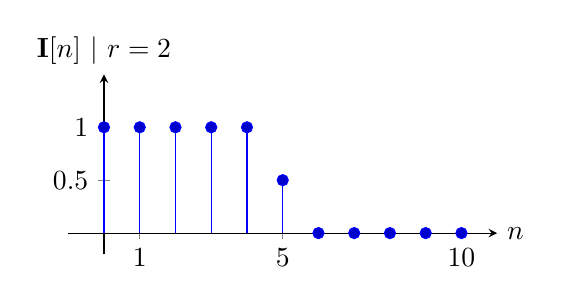
\begin{tikzpicture}
\begin{axis} [width=200pt,height=110pt,
	axis x line=middle, 
	axis y line=middle, 
	tick align=center,
	every axis x label/.style={at={(current axis.right of origin)},anchor=west},
	every axis y label/.style={at={(current axis.above origin)}, anchor=north east,above=0mm},
	xmin=-1, xmax=11,
	xtick={0, 1, 5, 10},
	xlabel=$n$,
	ymin=-0.2, ymax=1.5,
	ytick={0, 0.5, 1},
	ylabel={$\img [n]  ~|~  r=2$},
	color=black]
\addplot+[ycomb] plot coordinates {(0, 1) (1, 1) (2, 1) (3, 1) (4, 1) (5, 0.5) (6, 0) (7, 0) (8, 0) (9, 0) (10, 0)};
\end{axis} 
\end{tikzpicture}
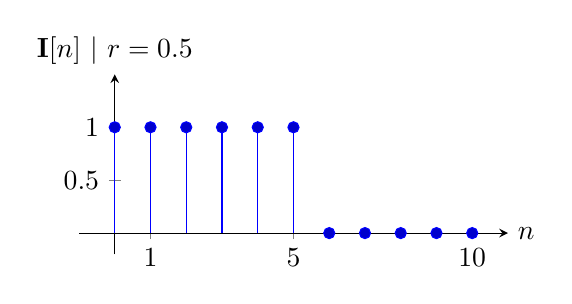
\begin{tikzpicture}
\begin{axis} [width=200pt,height=110pt,
	axis x line=middle, 
	axis y line=middle, 
	tick align=center,
	every axis x label/.style={at={(current axis.right of origin)},anchor=west},
	every axis y label/.style={at={(current axis.above origin)}, anchor=north east,above=0mm},
	xmin=-1, xmax=11,
	xtick={0, 1, 5, 10},
	xlabel=$n$,
	ymin=-0.2, ymax=1.5,
	ytick={0, 0.5, 1},
	ylabel={$\img [n]  ~|~ r=0.5$},
	color=black]
\addplot+[ycomb] plot coordinates {(0, 1) (1, 1) (2, 1) (3, 1) (4, 1) (5, 1) (6, 0) (7, 0) (8, 0) (9, 0) (10, 0)};
\end{axis} 
\end{tikzpicture}
}
\caption{Reconstructed signal using (left) $r=2$ and (right) $r=0.5$. The estimated values of $a$ are 0.5 and 1.} 
\label{fig:best_a}
\end{figure}



%%% HEEGER/BERGEN was here.

\subsection{Image Denoising (Bayesian Image Estimation)}

The highly kurtotic distribution of band-pass filter responses in images provides a regularity that is very useful for image denoising.  
If we assume zero-mean additive Gaussian noise of variance $\sigma^2$, and the observed subband coefficient value $\hat{x} = \hat\img_0 [n,m]$, where $\hat\img_0 [n,m]$ is the subband of the observed noisy input image, then the likelihood of any coefficient value, $x=\img_0 [n,m]$, is
\begin{equation}
p(\hat{x} \given x) \propto \exp{ \left( -\frac{(x - \hat{x})^2}{2 \sigma^2} \right) }, 
\end{equation}
where we are suppressing the normalization constants of \eqn{\ref{eq:derdist}} for simplicity.
The prior probability of any coefficient value is the Laplacian distribution (assuming $r=1$) of the subbands,
\begin{equation}
p(x) \propto \exp{ \left( -\frac{\left| x \right|}{s} \right) }.
\end{equation}
By Bayes rule, the posterior probability is the product of those two functions, 
\begin{equation}
P(x \given \hat{x}) \propto \exp{ \left( -\frac{\left| x \right|}{s} \right)} \exp{ \left( -\frac{(x - \hat{x})^2}{2 \sigma^2} \right) }
\label{eq:posterior_w_given_y}
\end{equation}

The plots of \fig{\ref{fig:waveletBayes}} show how this works.  The horizontal axis for each plot is the value at a pixel of an image subband coefficient.  The blue curve, showing the Laplacian prior probability for the subband values, is the same for all rows. The red line is the Gaussian likelihood and it is centered in the observed coefficient, and it is proportional to the probability that the true value had any other coefficient value. The green line shows the posterior, \eqn{\ref{eq:posterior_w_given_y}}, for several different coefficient observation values.  \Fig{\ref{fig:waveletBayes}}{a} shows the result when a zero subband coefficient is observed, resulting in the zero-mean Gaussian likelihood term (red), and the posterior (black) with a maximum at zero.  In \fig{\ref{fig:waveletBayes}}{b} an observation of 0.26 shifts the likelihood term, but the posterior still has a peak at zero.  And in \fig{\ref{fig:waveletBayes}}{c} an observed coefficient value of 1.22 yields a maximum posterior probability estimate of 0.9.


\begin{figure}
\centerline{
\includegraphics[width=.9\linewidth]{figures/statistical_image_models/wavelet_denoising.eps}
}
%\includegraphics[width=0.7\linewidth]
%{figures/statistical_image_models/x0wavelet.pdf}}
%\centerline{
%\includegraphics[width=0.7\linewidth]
%{figures/statistical_image_models/x1wavelet.pdf}}
%\centerline{
%\includegraphics[width=0.7\linewidth]
%{figures/statistical_image_models/x3wavelet.pdf}}
\caption{Showing the likelihood, prior, and posterior terms for the estimation of a subband coefficient from several noisy observations.  (a)  A zero subband coefficient is observed. (b)  An observation of 0.26 shifts the likelihood term, but the posterior still has a peak at zero. (c) an observed coefficient value of 1.22 yields a maximum posterior probability estimate of 0.9.
}
\label{fig:waveletBayes}
\end{figure}


\Fig{\ref{fig:bayeslut}} shows the resulting look-up table to modify the noisy observation to the MAP estimate for the denoised coefficient value.  Note that this implements a {\bf coring function} \cite{Simoncelli96}:  if a coefficient value is observed near zero, it is set to zero, based on the very high prior probability of zero coefficient values. 


\begin{figure}
\centerline{
\includegraphics[width=0.4\linewidth]{figures/statistical_image_models/waveletlut.pdf}
}
\caption{Input/output coring curve for maximum posterior denoising for the example of \fig{\ref{fig:waveletBayes}}.
}
\label{fig:bayeslut}
\end{figure}

For a more detailed analysis and examples of denoising using the Laplacian image prior, we refer the reader to the work of Eero Simoncelli \cite{Simoncelli96}.

\section{Nonparametric Markov Random Field Image Models}

The Gaussian and kurtotic wavelet image priors both involve modeling the image as a sum of statistically independent basis functions, Fourier basis functions, in the case of the Gaussian model, or wavelets, in the case of  the wavelet image prior. 

A powerful class of image models is known as {\bf Markov random field} (MRF) models.  They have a precise mathematical form, which we will describe later, in \chap{\ref{chapter:probabilistic_graphical_models}}.  For now, we present the intuition for these models:  if the values of enough pixels surrounding a given pixel are specified, then the probability distribution of the given pixel is independent of the other pixels in the image.  To fit and sample from the MRF structure requires the mathematical tools of graphical models, to be introduced in \chap{\ref{chapter:probabilistic_graphical_models}}.

%, but here we present an algorithm, introduced by Efros and Leung \cite{Efros99} that exploits intuitions about the Markov structure of images to synthesize textures that are visually compelling.  



%\subsection{Denoising model (Non-local Means)}
%The image generation method of Efros and Leung has a natural denoising counterpart.  
As we will see in the following chapter,  Efros and Leung \cite{Efros99} introduced an algorithm for texture synthesis that exploits intuitions about the Markov structure of images to synthesize textures that are visually compelling.
The intuition of the Efros and Leung texture generation model is that if you condition on a large enough region of nearby pixels around a center pixel, that effectively determines the value of the central pixel. We will study this algorithm in more detail in the next chapter devoted to texture analysis and synthesis (\chap{\ref{chap:textures}}). We will focus here on a similar algorithm for the problem of image denoising.  

\subsection{Denoising Model (Nonlocal Means)}

Baudes, Coll, and Morel made use of that intuition to define the {\bf nonlocal means} denoising algorithm \cite{Baudes2005}. \index{Nonlocal means}
The nonlocal means denoised image is a weighted sum of all other pixels in the image, weighted by the similarity of the local neighborhoods of each pair of pixels.  More formally, 
\begin{equation}
    \img_{\mbox{NLM}}[n,m] = \sum_{k,l} w_{n,m}[k,l] \img [k,l]
\end{equation}
where
\begin{equation}
    w_{n,m}[k,l] = \frac{1}{Z_{n,m}} \exp{\frac{- \left| \img [N_{k,l}] - \img [N_{n,m}] \right| ^2}{h^2}},
    \label{fig:mask}
\end{equation}
where $N_{i, j}$ denotes an $h \times h$ region of pixels centered at $i, j$, and $Z_{n,m}$ is set so that the weights over the image sum to one, that is $\sum_{kl} w_{n,m}[k,l] = 1$.


%Left:  original image.  Middle: With additive Gaussian noise added, $\sigma=15$ for 0-255 image scale. Left: Non-local means noise removed result. 

% **********************
% august 29, 2021.  see numtour.m   to do:  look at the histograms (change the figs flag) for meanFlag = 0 % and nois level = 0.0111.  do these parameters make visual sense with all the plots??
% **********************



\Fig{\ref{fig:nlm1}} shows the weighting functions for two images. The parameter $h$ is typically set to $10 \sigma $, where $\sigma$ is the estimated image noise standard deviation. Within figures \ref{fig:nlm1}(a and b) at left is a grayscale image where the center position of interest to be denoised is marked with a white star.  The right side of the figures shows for some value of $h$ in \eqn{\ref{fig:mask}} the weighting function $w_{n,m}[k,l]$ indicating which pixels are averaged together to yield the nonlocal mean value placed at the starred location in the denoised image.  Note, for both figures \ref{fig:nlm1}(a and b) the sampling at image regions with similar local structure as the image position to be denoised.


\begin{figure}[t]
\centerline{
\sublabel{a}{\includegraphics[width=0.48\linewidth]{figures/statistical_image_models/nlm1a.jpg}}
\sublabel{b}{\includegraphics[width=0.48\linewidth]{figures/statistical_image_models/nlm1b.jpg}}
}
\caption{Regions of support for the nonlocal means denoising algorithm. 
{\em Source:} Image from \cite{Baudes2005}.}
\label{fig:nlm1}
\end{figure}

\Fig{\ref{fig:nlm2}} shows the result on a real image.  On the left is the original image. The middle image is with additive Gaussian noise added, that is, $\sigma=15$ for 0–255 image scale. On the right is the result, showing the image with nonlocal means noise removed.


\begin{figure}[t]
\centerline{
\includegraphics[width=1\linewidth]{figures/statistical_image_models/nlmresult.jpg}
}
\caption{Nonlocal means denoising algorithm results. (left) Original image without noise. (middle) Noisy image. (right) Denoised image. {\em Source:} Figure from \cite{Baudes2011}.
}
\label{fig:nlm2}
\end{figure}


% Observations: if $r = 2$, then this model becomes the gaussian model.


%\subsubsection{Examples}
%
%
%Example of a 1D step edge and sharpening. See the effect of p in what is the best solution.
%

% First, what is the most likely image under the model eq.~\ref{eq:waveletmodel}. It is a constant image. 

%\begin{examples} {\bf step edge}

% To build an intuition on what types of image structures are more likely under the wavelet marginal model, let's consider a simple 1D image:
% \begin{equation}
% \img = \left[1,~ 1,~ 1,~ a,~ 0,~ 0,~ 0\right]
% \end{equation}
%Different values of $a$ will produce different types of steps. For instance, setting $a=1$ or $a=0$ will produce a sharp step edge. Setting $a=0.5$ will produce a smooth step signal. What is the value of $a$ that maximizes the probability of this 1D image under the wavelet marginal model? 

%First we need to specify the prior distribution. For this example we will use a model specified by a single filter with the form $[-1, 1]$, and we will use the distribution given by eq.~\ref{eq:derdist}. In this case, we can write the wavelet marginal model in close form. Applying the filter $\left[-1, 1\right]$ to the 1D signal and using mirror boundary conditions, results in:
%\begin{equation}
%h(\img) = \left[0,~0,~ 0,~ 1-a,~ a,~ 0,~ 0\right]
%\end{equation}

%Now, we can use Eq.~\ref{eq:waveletmodel} and obtain the probability of $\img$ as a function of $a$:
%\begin{eqnarray}
%p(\img) = \prod_{x} p(h(\img, x)) = \\
%\frac {\exp \left(- \left| (1-a)/s  \right|^r \right) \exp \left(- \left| a/s  %\right|^r \right)}{(2s/r \Gamma(1/r))^7} = \\
%\frac{1}{(2s/r \Gamma(1/r))^7} \exp - \frac{\left| 1-a \right|^r+\left| a %\right|^r} {s^r}  
%\end{eqnarray}
%the first factor only depends on $r$. The second factor depends on $a$ and $r$. We are interested in seeing the values of $a$ that maximize $p(\img)$ for each value of $r$. Therefore, only the second factor is important for this analysis. The next figure plots the value of the second factor as we vary $a$ and $r$. The red line represent the places where the function reaches a maximum as a function of $a$ for each value of $r$.

%\begin{figure}[htpb]
%\centerline{
%\includegraphics[width=.6\linewidth]{figures/statistical_image_models/best_a_s1.eps}
%} 
%\caption{Best values of $a$ that maximize the probability of the 1D image %$\left[1,~ 1,~ 1,~ a,~ 0,~ 0,~ 0\right]$ under the wavelet prior model.} 
%\label{fig:best_a}
%\end{figure}

%For $r=2$ the best value of $a$ is $a=0.5$, and this solution is the best for any value of $r>1$. For $r=1$, any value $a \in \left[0,1\right]$ is equally good, and $p(\img)$ decreases for values of $a$ outside that range. And for $r<1$, the best solution is for $a=0$ or $a=1$. Therefore, values of $r<1$ prefer sharp step edges. Note that $a=0$ and $a=1$ are both the same step edge translated by one pixel. 

%\end{examples} 
%
%\begin{examples}
%What happens if the signal has the form: $\img = \left[0,~ 1,~ 2,~ a,~ 4,~ 5,~ 6\right]$
%\end{examples} 
%
%\begin{examples}
%What happens if the signal has the form: $\img = \left[0,~ 0,~ 0,~ a,~ 0,~ 0,~ 0\right]$. (solution: $a=0$ for all $r$).
%\end{examples} 
%
%\begin{examples}
%What happens if we define other filters than $\left[-1, 1\right]$. For instance $\left[-1,~ 2,~ -1\right]$.
%\end{examples} 
%
%\example{Superresolution}
%
%\begin{equation}
%{\bf a} = [a_0,~a_1,~ a_2,~ a_3,~ a_4,~ a_5,~ a_6,~a_7]
%\end{equation}
%
%but we observe the signal:
%\begin{equation}
%{\bf b} = [b_0,~ b_1,~ b_2,~ b_3]
%\end{equation}
%obtained by filtering $\bf a$ with a filter $[1,~1]$ and then downsampling by a factor of 2. The process of going from $\bf a$ to $\bf b$ is linear.
%\begin{eqnarray*}
%b_0 = a_0+a_1\\
%b_1 = a_2+a_3\\
%b_2 = a_4+a_5\\
%b_3 = a_6+a_7\\
%\end{eqnarray*}
%
%Our goal is to recover the signal $\bf a$.
%
%\begin{equation}
%\bf a ^* = argmax_{\bf a} P(\bf a ~|~ \bf b)  = \frac{P(\bf b ~|~ \bf a) P(\bf a)}{P(\bf b)}
%\end{equation}
%
%If we consider only the feasible solutions, then the only term that matters to select the solution is the prior $P(\bf a)$.
%
%\begin{equation}
%h({\bf a}) = [0,~a_1-a_0,~ a_2-a_1,~ a_3-a_2,~ a_4-a_3,~ a_5-a_4,~ a_6-a_5,~ a_7-a_6]
%\end{equation}
%
%\begin{equation}
%h({\bf a}) = [0,   ~b_0-2 a_0, ~
%                    a_2-a_1,~ b_1-2 a_2,~ 
%                    a_4-a_3,~ b_2- 2 a_4,~ 
%                    a_6-a_5,~ b_3- 2 a_6]
%\end{equation}
%
%\begin{eqnarray}
%\log p({\bf a}) = \sum_{x} \log p(h(\bf a, x)) = \\
%- \left | (b_0-2 a_0)/s  \right|^r
%- \left | (a_2-a_1)/s  \right|^r - \left | (b_1-2 a_2)/s  \right|^r
%- \left | (a_4-a_3)/s  \right|^r - \left | (b_2-2 a_4)/s  \right|^r
%- \left | (a_6-a_5)/s  \right|^r - \left | (b_3-2 a_6)/s  \right|^r
%\end{eqnarray}

%\begin{examples}{\bf Image impainting}
%
%2D image with a missing block in the center.
%
%It is like having boundary conditions.
%
%$I = I_b \cup I_c$
%
%$p(I_c ~|~ I_b)$
%\end{examples}
%
%\begin{examples}{\bf Most natural image}
%Find the image from a database that maximizes the prior... What is the most natural image? Figure: show sorted images according to the prior.
%\end{examples}
%
%
%\begin{examples}{\bf Superresolution}
%One example for which we can not derive things analytically. Use iterative weighted least square to do inference. Check effect on the exponent p on the solution.
%\end{examples}
%
%


%\section{Sparsity}

%Talk about Field and Olshausen, and establish parallelism with CNN.


%\subsubsection{Cooring: Denoising with the wavelet model}

%Deduce Wavelet thresholding using the bayesian model.

%In the case of $\left[-1, 1\right]$ derivatives we can transform the image, then apply the prior to the derivatives, and then reverse the transformation. 

%
%\subsubsection{Retinex}
%
%Try a sequence of models:
%
%1) gaussian
%
%2) laplacian
%
%3) laplacian + gaussian on second order derivatives
%
%
%
%is one step beyond denoting...
%
%Craik-O'Brien-Cornsweet effect
%
%
%\begin{figure}[htpb]
%\centerline{
%\includegraphics[width=1\linewidth]{figures/statistical_image_models/Cornsweeteffect.eps}
%} 
%\caption{Cornsweet effect.} 
%\label{fig:Cornsweeteffect}
%\end{figure}
%




%\subsection{Gaussian scale mixtures}


%\section{Patch based models}
%
%How do non-parametric image models fit in this?







%\section{Generative models in vision}
%
%As a more challenging task: a really complete model. Can it be done? I think there is a CNN by Renato trying to build also priors for images. Describe it here.
%
%Explaining away, sufficient statistics, nuisance parameters, ...

%
%
%\section{Applications of statistical image models}
%
%
%\subsection{Camera motion removal}
%
%\subsection{Separating image into intrinsic images}
%
%\subsection{Color demosaicing}
%
%
\section{Concluding Remarks}

The models presented in this chapter do not try to understand the content of the pictures, but utilize low-level regularities of images in order to build a statistical model.  Modeling these statistical regularities enable many tasks, including both image synthesis and image denoising.

We have see some simple models that try to constrain the space of natural images. These models, despite their simplicity, are useful in several applications. However, they fail in providing a strong image model that can be used to sample new images. As illustrated in \fig{\ref{fig:spaces_real_images_final}} the sequence of models we have studied in this chapter, only help in reducing a bit the space of possible images.


\begin{figure}
\centerline{
\includegraphics[width=1\linewidth]{figures/statistical_image_models/spaces_real_images_and_models_final.eps}
} 
\caption{The space of natural images is just very small part of the space of all possible images. In the case of color images with $32\times32$ pixels, most of the space is filled with images that look like noise.} 
\label{fig:spaces_real_images_final}
\end{figure}

We will see stronger generative image models in \chap{\ref{chapter:generative_models}}.

\begin{comment}
Figure~\ref{fig:synthesis} shows a random draw from the kurtotic wavelet statistical model of images \cite{Simoncelli2005}.  The long tails of the Laplacian subband distributions results in a small number of high-amplitude wavelet basis functions.  For the subband representation used here, the basis functions are x-y separable, giving the large amplitude, large-scale wavelets visible in the image.


\begin{figure}[htpb]
\centerline{
{\includegraphics[width=0.3\linewidth]{figures/statistical_image_models/waveletEero.pdf}}}
\caption{Random draw from wavelet model  \cite{Simoncelli2005}, for an x-y separable model composed of wavelets of many spatial scales.  Figure permission.
}
\label{fig:synthesis}
\end{figure}

\end{comment}  % bill's edits to antonio's chapter
% \include{chapters/bill/applics_stat_image_models}
%% %\setcounter{chapter}{30}
\chapter{Probabilistic Graphical Models}
\label{chapter:probabilistic_graphical_models}
% aug. 23, 2019  billf renamed from "tiny_graphical_models"
%\reviewcomment{Readable but unfinished. Figures need to be reformatted and missing references.}



\section{Introduction}

{\bf Probabilistic graphical models} describe joint probability
distributions in a modular way that allows us to reason about the
visual world even when we're modeling very complicated situations.
These models are useful in vision, where we often need to exploit
modularity to make computations tractable.

A probabilistic graphical model is a graph that describes a class of
probability distributions sharing a common structure.  The graph
has nodes, drawn as circles, indicating the variables of the joint
probability.  It has edges, drawn as lines connecting nodes
to other nodes.  At first, we'll restrict our attention to a type of
graphical model called undirected, so the edges are line segments
without arrowheads.

In undirected graphical models, the edges indicate the conditional independence structure of
the nodes of the graph.  If there is no edge between two nodes, then
the variables described by those nodes are independent, conditioned on the values of intervening nodes in
any path between them in the graph.  If two nodes do have a line between
them, then we cannot assume they are independent.  We
introduce this through a set of examples.  

%\clearpage

\section{Simple Examples}
Here is the simplest probabilistic graphical model:
\begin{figure}
\centerline{\includegraphics[width=0.08\linewidth]{figures/graphical_models/x1.pdf}}
\caption{A graphical model with only one node.}
\end{figure}

This {\bf graph}
\index{Graph}
is just a single node for the variable $x_1$.  There is no restriction
imposed by the graph on the functional form of its probability function.
In keeping with notation we'll use later, we write that the
probability distribution over $x_1$, $p(x_1) = \phi_1(x_1)$.

Another trivial graphical model is this:
\begin{figure}
\centerline{\includegraphics[width=0.2\linewidth]{figures/graphical_models/x1x2.pdf}} 
\caption{Two independent variables.}
\end{figure}

Here, the lack of a
line connecting $x_1$ with $x_2$ indicates a lack of statistical
dependence between these two variables.  In detail, we condition on knowing the
values of any connecting neighbors of $x_1$ and $x_2$ (in this case there
are none) and thus $x_1$ and $x_2$ are statistically independent.  Because of
that independence, the joint probability depicted by this graphical
model must be a product of each variable's marginal probability and thus
must have the form:  $p(x_1, x_2) = \phi_1(x_1) \phi_2(x_2) $.

Let's add a line between these two variables:
\begin{figure}
\centerline{\includegraphics[width=0.16\linewidth]{figures/graphical_models/x1bx2.pdf}} 
\caption{Two dependent variables.}
\end{figure}

By that graph, we
mean that there may be a statistical dependency between
the two variables.  The class of probability
distributions depicted here is now more general than the one above, and we can
only write that the joint probability as some unknown function of
$x_1$ and $x_2$, $p(x_1, x_2) = \phi_{12}(x_1, x_2)$.  This graph
offers no simplification from the most general probability function of
two variables.

Here is a graph with some structure:
\begin{figure}
\centerline{\includegraphics[width=0.24\linewidth]{figures/graphical_models/x1bx2bx3.pdf}} 
\caption{Three dependent variables.}
\label{graph:3node}
\end{figure}

This graph means that if we condition on the variable $x_2$,
then $x_1$ and $x_3$ are independent.  A general form for
$p(x_1, x_2, x_3)$ that guarantees such conditional independence is
\begin{equation}
p(x_1, x_2, x_3) =  \phi_{12}(x_1, x_2)  \phi_{23}(x_2, x_3).
\label{eq:x1x2x3}
\end{equation}
Note the conditional independence implicit in \eqn{\ref{eq:x1x2x3}}:  if the value of $x_2$ is given
(indicated by the solid circle in the graph below), then
the joint probability of \eqn{\ref{eq:x1x2x3}} becomes a product of
some function $f(x_1)$ times some other function $g(x_3)$, revealing
the conditional independence of $x_1$ and $x_3$.  Graphically, we denote the conditioning on the variable $x_2$ with a filled circle for that node:
\begin{figure}
\centerline{\includegraphics[width=0.26\linewidth]{figures/graphical_models/3node.pdf}} 
\caption{Conditioning on the variable $x_2$ is indicated by the filled circle.}
\label{graph:3node2}
\end{figure}

We will exploit that structure of the joint
probability to perform inference efficiently using an algorithm called belief propagation (BP).

A celebrated theorem, the {\bf Hammersley-Clifford theorem} \cite{Hammersley1971}, tells 
the form the joint probability must have for any given graphical model.
The joint probability for a probabilistic graphical model must be
a product of functions of each the {\bf maximal cliques} 
\index{Maxima cliques}
of the
graph.  Here we define the terms.

A {\bf clique}
\index{Clique}
is any set of nodes where each node is connected to
every other node in the clique.  These graphs illustrate the 
clique property:
\begin{figure}
\centerline{\includegraphics[width=0.5\linewidth]{figures/graphical_models/cliques1.pdf}}
\caption{A clique is any set of nodes where each node is connected to
every other node in the same clique.}
\end{figure}

A {\bf maximal clique}
\index{Maximal clique} is a clique that
can't include more nodes of the graph without losing the clique property.
The sets of nodes below form maximal cliques (left), or do not (right):
\begin{figure}
\centerline{\includegraphics[width=0.4\linewidth]{figures/graphical_models/cliques2.pdf}}
\caption{A maximal clique is the largest possible clique.}
\end{figure}

The {\bf Hammersley-Clifford theorem} \cite{Hammersley1971}
states that a positive probability distribution has the independence structure described by
a graphical model if and only if it can be written as a product of functions
over the variables of each maximal clique:
\begin{equation}
p(x_1, x_2, \ldots, x_N) =  \prod_{x_c  \in x_i} \Psi_{c} (x_c),
\end{equation}
where the product is over all maximal cliques $x_c$ in the graph, $x_i$.

In the example of graph in \fig{\ref{graph:3node}}, the maximal cliques  are (x1,
x2) and (x2, x3), so the Hammersley-Clifford theorem says that the
corresponding joint probability must be of the form of
\eqn{\ref{eq:x1x2x3}}. 

Now we examine some graphical model structures that are especially useful in vision.
In perception problems, we typically have both observed and 
unobserved variables.  The graph below shows a simple {\bf Markov chain} \cite{Gagniuc1989} \index{Markov chain} structure
with three observed variables, shaded, labeled $y_i$, and three
unobserved variables, labeled $x_i$:
\begin{figure}
\centerline{\includegraphics[width=0.36\linewidth]{figures/graphical_models/x1x2x3y1y2y3.pdf}} 
\caption{Markov chain  with three observed variables, shaded, and three unobserved variables.}
\label{fig:chain}
\end{figure}

This is  a chain because
the variables form a linear sequence.  It's a Markov chain structure because the
hidden variables have the Markov property:  conditional on 
 $x_2$, variable $x_3$ is independent of variable $x_1$.  The joint
probability of all the variables shown here is
$p(x_1, x_2, x_3, y_1, y_2, y_3) =  \phi_{12}(x_1, x_2)  \phi_{23}(x_2, x_3)
\psi_{1}(y_1, x_1) \psi_{2}(y_2, x_2) \psi_{3}(y_3, x_3) $.   Using
$p(a,b) = p(a \given b) p(b)$, we can
also write the probability of the $x$ variables conditioned on the
observations $y$,
\begin{equation}
p(x_1, x_2, x_3 \given y_1, y_2, y_3) =  
\frac{1}{p(\mathbf{y})} \phi_{12}(x_1, x_2)  \phi_{23}(x_2, x_3) \psi_{1}(y_1, x_1) \psi_{2}(y_2, x_2) \psi_{3}(y_3, x_3). 
\end{equation}
For brevity, we write $p(\mathbf{y})$ for $p(y_1, y_2, y_3)$.  Thus, to
form the conditional distribution, within a normalization factor, we simply include the observed variable
values into the joint probability.
For vision applications, we often use such Markov chain structures to
describe events over time.  


To capture relationships over space, a two-dimensional (2D)
structure is useful, called a {\bf Markov random field} (MRF) 
\index{Markov random field}
\cite{Blake2011}:
\begin{figure}
\centerline{\includegraphics[width=0.48\linewidth]{figures/graphical_models/mrf.pdf}} 
\caption{Two-dimensional Markov random field.}
\end{figure}

Then the joint probability over all the variables factorizes into this product:
\begin{equation}
p(\mathbf{x} \given \mathbf{y}) = 
\frac{1}{p(\mathbf{y})}
\prod_{(i,j)} \phi_{ij}(x_i, x_j) \prod_i \psi_i(x_i, y_i),
\end{equation}
where the first product is over all spatial neighbors $i$
and $j$, and the second product is over all nodes $i$.

\begin{comment}
\begin{figure}
\centerline{
\sublabel{a}{\epsfig{file=figures/graphical_models/leaf2.jpg,width=2.2in}}
\sublabel{b}{\epsfig{file=figures/graphical_models/leaf3.jpg,width=2.2in}}}
%\sublabel{c}{\epsfig{file=figures/graphical_models/leaf1,width=1.4in}}}
\centerline{
%\hspace{1in}
\sublabel{c}{\epsfig{file=figures/graphical_models/leaf1,width=4.4in}}}
\caption{(a) Image to be segmented. (b) A local region of (a).  (c) Visualization of an MRF of nodes corresponding to image pixels, with states indicating segment membership, for a hypothetical most probable configuration.}
\label{fig:leafs}
\end{figure}
\end{comment}



An example of how Markov random field models are applied to images is depicted in \fig{\ref{fig:leafs}}, which show a small image region and its context in the image (\fig{\ref{fig:leafs}}[a]). \Fig{\ref{fig:leafs}}(b) shows an MRF with each node corresponding to a pixel of the image region.  The states of an MRF can be indicator variables of image segment membership for each pixel. The states of a hypothetical most-probable configuration of this MRF are shown as the color of each node in this illustration.


\begin{figure}
\centerline{
\sublabel{a}{\epsfig{file=figures/graphical_models/leaf2.jpg,width=2.3in}}
\sublabel{b}{\epsfig{file=figures/graphical_models/leaf1,width=2.5in}}}
\caption{(a) Image to be segmented and a local region of (a) marked in red.  (b) Visualization of an MRF of nodes corresponding to image pixels inside the marked region, with states indicating segment membership, for a hypothetical most probable configuration.}
\label{fig:leafs}
\end{figure}

%\clearpage

\section{Directed Graphical Models}


In addition to undirected graphical models, another
type of graphical  model is commonly used.
{\bf Directed graphical models} \cite{Koller2009} describe factorizations of the joint
probability into products of conditional probability distributions.  
Each node in a directed graph contributes a
well-specified factor in the joint probability:  the probability of
its variable, conditioned all the variables originating arrows
pointing into it.  So this graph
\begin{figure}
\centerline{\includegraphics[width=0.20\linewidth]{figures/graphical_models/directed.pdf}} 
\caption{A directed graphical model with three variables.}
\end{figure}

\noindent denotes the joint probability, 
\begin{equation}
p(x_1, x_2, x_3) = p(x_2)  p(x_1 \given x_2) p(x_3 \given x_2) 
\label{eq:directedjoint}
\end{equation}

The general rule for writing the joint probability described by a
directed graph is this:  Each node, $x_n$, contributes the factor
$p(x_n \given x_{\Xi})$, where $\Xi$ is the set of nodes with arrows pointing
in to node $x_n$.  You can verify that \eqn{\ref{eq:directedjoint}}
follows this rule.  Directed graphical models are often used to describe causal processes.

\section{Inference in Graphical Models}

Given a probabilistic graphical model and observations, we want to estimate the states of 
the unobserved variables. For example, given image
observations, we may want to estimate the pose of the person.
The {\bf belief propagation} algorithm lets us do that efficiently.

\index{Bayes' theorem}
Recall the Bayesian inference task:  our observations are the
elements of a vector, $\mathbf{y}$, and we seek to infer the probability
$p(\mathbf{x} \given \mathbf{y})$ of some scene
parameters, $\mathbf{x}$, given the observations. 
By Bayes' theorem, we have
\begin{equation}
p(\mathbf{x} \given \mathbf{y}) = \frac{p(\mathbf{y} \given \mathbf{x}) p(\mathbf{x}) }{p(\mathbf{y}) }
\end{equation}
The {\bf likelihood term} 
\index{Likelihood}
$p(\mathbf{y} \given \mathbf{x})$ describes how a
rendered scene $\mathbf{x}$ generates observations $\mathbf{y}$.  The {\bf
prior probability}, 
\index{Prior probability}
$p(\mathbf{x})$, tells the probability of any given
scene $\mathbf{x}$ occurring.  For inference, we often ignore the denominator,
$P(\mathbf{y})$, called the {\bf evidence}, as it is constant with
respect to the variables we seek to estimate, $\mathbf{x}$.

\marginnote{The statistician Harold Jeffreys wrote, "Bayes' theorem is to the theory of probability what Pythagorus' theorem is to geometry" \cite{Jeffreys1973}}

Typically, we make many observations, $\mathbf{y}$, of the variables of some system,
and we want to find the the state of some hidden variable, $\mathbf{x}$, given those
observations.  The posterior probability, $p(\mathbf{x} \given \mathbf{y})$, tells
us the probability for any value of the hidden variables, $\mathbf{x}$.
From this posterior probability, we often want some single {\em best} estimate for $\mathbf{x}$,
denoted $\mathbf{\hat{x}}$ and called a point estimate.  

Selecting the best estimate $\mathbf{\hat{x}}$ requires specifying a
penalty for making a wrong guess. If we penalize all wrong answers
equally, the best strategy is to guess the value of  $\mathbf{x}$ that maximizes
the posterior probability, $p(\mathbf{x} \given \mathbf{y})$ (because any other
explanation $\mathbf{\hat{x}}$ for the observations $\mathbf{y}$  would be
less probable).  That is called the {\bf maximum a posteriori} (MAP) estimate.
\index{Maximum a posteriori}

But we may want to penalize wrong answers as a function of how far
they are from the correct answer.  If that penalty function is
the squared distance in $\mathbf{x}$, then the point estimate that
minimizes the average value of that error is called the {\bf minimum mean squared error}
estimate (MMSE).
\index{Minimum mean squared error}
To find this estimate, we seek 
the $\hat{\mathbf{x}}$ that minimizes the squared error, weighted by the probability of each outcome:
\begin{equation}
\hat{\mathbf{x}}_{MMSE} = \mbox{argmin}_{\tilde{\mathbf{x}}} 
\int_{\mathbf{x}} p(\mathbf{x} \given \mathbf{y}) (\mathbf{x}-\tilde{\mathbf{x}})'
(\mathbf{x}-\tilde{\mathbf{x}}) d\mathbf{x}
\end{equation} 
Differentiating with respect to $\mathbf{x}$ to solve for the stationary
point, the global minimum for this convex function, we find
\begin{equation}
\hat{\mathbf{x}}_{MMSE} = \int_{\mathbf{x}} \mathbf{x} p(\mathbf{x} \given \mathbf{y})  d\mathbf{x}.
\end{equation}
Thus, the minimum mean square error estimate, $\hat{\mathbf{x}}_{MMSE}$,
is the mean of the posterior distribution.  
If $\mathbf{x}$ represents a discretized space, then the
marginalization integrals over $d\mathbf{x}$ become sums over the
corresponding discrete states of $\mathbf{x}$.

\marginnote{For a Gaussian probability distribution, the MAP estimate and the MMSE estimate
are always the same, since the mean of the distribution is always its maximum value.}

For now, we'll assume we seek the MMSE estimate. By the properties of
the multivariate mean, to find the mean at each variable, or node, in
a network, we can first find the marginal probability at each node,
then compute the mean of each marginal probability.  In other words,
given $p(\mathbf{x} \given \mathbf{y})$, we will compute $p(x_i \given \mathbf{y})$,
where $i$ is the $i$-th hidden node.  From $p(x_i \given \mathbf{y})$ it is
simple to compute the posterior mean at node $i$.

For the case of discrete variables, we compute the marginal probability at a node by summing over the states at all the other nodes,
\begin{equation}
    p(x_i \given \mathbf{y}) =  \sum_{j  \mbox{\textbackslash} i} \sum_{x_j} 
    p(x_1, x_2, \ldots, x_i, \ldots, x_N \given \mathbf{y}),
    \label{eq:discreteMarginalization}
\end{equation}
where the notation $j \mbox{\textbackslash} i$ means ``all possible values of $j$ except for $j = i$.''

\section{Simple Example of Inference in a Graphical Model}
\label{sect:simpleexample}

To gain intuition, let's calculate the marginal probability for a
simple example.  Consider the three-node Markov chain 
of \fig{\ref{fig:chain2}}.
\begin{figure}
\centerline{\includegraphics[width=0.36\linewidth]{figures/graphical_models/x1x2x3y1y2y3.pdf}} 
\caption{Same three-node Markov chain of \fig{\ref{fig:chain}}.}
\label{fig:chain2}
\end{figure}

Vision tasks this can apply to include modeling the probability of a pixel
belonging to an object edge, given the evidence, observations $\mathbf{y}$, at a point and two
neighboring locations.  The inferred states $\mathbf{x}$ could be a label
indicating the presence of an edge.

We seek to marginalize the joint probability in order to
find the marginal probability at node 1, $p(x_1 \given \mathbf{y})$, given
observations $y_1$, $y_2$, and $y_3$, which we denote as $\mathbf{y}$.
We have, assuming the nodes have discrete states,
\begin{equation}
p(x_1 \given \mathbf{y}) = \sum_{x_2} \sum_{x_3}  p(x_1, x_2, x_3 \given \mathbf{y})
\label{eq:3chain}
\end{equation}

Here's the main point.  If we knew nothing about the structure of
the joint probability $p(x_1, x_2, x_3 \given \mathbf{y})$, the computation would require
$\left| x \right|^3$ computations: a double-sum over all $x_2$ and $x_3$ states must
be computed
for each possible $x_1$ state (we're denoting the number of states of any of the $x$
variables as $\left| x \right|$).  In the more general case, for a Markov chain of
$N$ nodes, we would need $\left| x \right|^N$ summations to compute the desired
marginal at any node of the chain.  Such a computation quickly
becomes intractable as $N$ grows.

But we can exploit the model's structure to avoid the
exponential growth of the computation with $N$.
Substituting the joint probability, from the graphical model, into the
marginalization equation, \eqn{\ref{eq:3chain}}, gives
\begin{equation}
p(x_1 \given \mathbf{y}) = 
\frac{1}{p(\mathbf{y})} \sum_{x_2} \sum_{x_3}  
\phi_{12}(x_1, x_2)  \phi_{23}(x_2, x_3) \psi_{1}(y_1, x_1) \psi_{2}(y_2, x_2) \psi_{3}(y_3, x_3) 
\label{eq:3chainb}
\end{equation}
This form for the joint probability reveals that not every variable is
coupled to every other one.  We can pass summations
through  variables they don't sum over, letting us compute the
marginalization much more efficiently.  This will make only a small
difference for this short chain, but it makes a huge difference
for longer ones.  So we write
\begin{eqnarray}
p(x_1 \given \mathbf{y}) 
& = & 
\frac{1}{p(\mathbf{y})} \sum_{x_2} \sum_{x_3}  
\phi_{12}(x_1, x_2)  \phi_{23}(x_2, x_3)
\psi_{1}(y_1, x_1) \psi_{2}(y_2, x_2) \psi_{3}(y_3, x_3)  
\label{eq:before}
\\
& = &
\frac{1}{p(\mathbf{y})}
\psi_{1}(y_1, x_1) 
\sum_{x_2} \phi_{12}(x_1, x_2) \psi_{2}(y_2, x_2) 
\sum_{x_3}   \phi_{23}(x_2, x_3)  \psi_{3}(y_3, x_3)  
\label{eq:after} 
\end{eqnarray}
That factorization of \eqn{\ref{eq:after}} is the key step.
It reduces the number of terms summed from order $\left| x \right| ^3$ to order $2
\left| x \right|^2$ for this chain, and for a chain of length $N$ chain, from order $\left|x \right|^N$ to order $(N-1) \left|x \right|^2$--from exponential to linear dependence on $N$--a
huge computational savings for large $N$.  

The partial sums of \eqn{\ref{eq:after}} are named  {\bf messages} 
\index{Message}
because they pass information from one node to another.  We call the message from node 3
to node 2, $m_{32}(x_2)  = \sum_{x_3}   \phi_{23}(x_2, x_3)
m_{63}(x_3) $.  The other partial sum is the message from node 2 to
node 1, 
$m_{21}(x_1)   = \sum_{x_2} \phi_{12}(x_1, x_2)  m_{52}(x_2)  
m_{32}(x_2) $.
Note that the messages are always messages about
the states of the node that the message is being sent to, that is, the
arguments of the message $m_{ij}$ are the states $x_j$ of node $j$.  The algorithm corresponding to \eqn{\ref{eq:after}} is called {\bf belief propagation}.

\Eqn{\ref{eq:after}} gives us the marginal probability at node 1.  To
find the marginal probability at another node, we 
can write out the sums over variables needed for that node, pass the
sums through factors in the joint probability that they don't operate
on, to come up with an efficient reorganization of summations analogous to
\eqn{\ref{eq:after}}.  We would find that many
of the summations from marginalization at the node $x_1$  would need
to be recomputed for the marginalization at node $x_2$.  That
motivates storing and reusing the messages, which the belief propagation algorithm does in an optimal way.

\section{Belief Propagation}

For more complicated graphical models, we want to 
replace the manual factorization above
with an automatic procedure for identifying the
computations needed for marginalizations and to 
cache them efficiently.  BP does that by
identifying those reusable sums, that is, the messages. 

\begin{figure}
\centerline{\includegraphics[width=0.5\linewidth]{figures/graphical_models/3bpc2.pdf}} 
\caption{Summary of the messages (partial sums) for a simple belief propagation example.} 
\label{fig:3bpc}
\end{figure}

\subsection{Derivation of Message-Passing Rule}
\label{sect:bpRules}

We'll describe belief propagation only for the special case of
graphical models with pairwise potentials.  
The clique potentials between neighboring nodes are $\psi_{ij}(x_j, x_i)$.
Extensions to higher-order
potentials is straightforward.  (Convert the
graphical model into one with only pairwise potentials.  This can be
done by augmenting the state of some nodes to encompass several others,
until the remaining nodes only need pairwise potential functions in
their factorization of the joint probability.)  You can find formal
derivations of belief propagation in \cite{Jordan98,Koller2009}.

Consider \fig{\ref{fig:bpmotivator2}}, showing a section of a general network with pairwise potentials.  There is a network of $N+1$
nodes, numbered $0$ through $N$ and we will marginalize over nodes
$x_1 \ldots x_N$.  \Fig{\ref{fig:bpmotivator2}}{a} shows the
marginalization equation for a network of variables with discrete states. (For continuous variables, integrals replace the summations). If we assume the nodes form a tree, we can
distribute the marginalization sum
past nodes for which the sum is a constant value to obtain the sums
depicted in \fig{\ref{fig:bpmotivator2}}{b}.  

We define a {\bf belief propagation message}:
A message $m_{ij}$, from node $i$ to node $j$, is the sum of the
 probability over all states of all
nodes in the subtree that leaves node $i$ and does not include node $j$.

Referring to \fig{\ref{fig:bpmotivator2}}{a}, shows the desired
marginalization sum over a network of pairwise cliques.   
We can pass the summations over node states through nodes that are
constant over those summations, arriving at the factorization shown in
\fig{\ref{fig:bpmotivator2}}{b}.  Remembering that the message from node $j$ to node $i$ is the sum
over the tree leaving node $j$, we can then read-off the recursive
belief propagation message update rule by marginalizing over the state probabilities at node $j$ in 
\fig{\ref{fig:bpmotivator2}}. As illustrated in \fig{\ref{fig:bpmotivator2}}, messages $m_{j+1,j}$ and $m_{kj}$ correspond to partial sums over nodes indicated in the graph: 
  $m_{j+1,j} = \sum_{x_{j+1} \ldots x_{k-1}}$ and 
  $m_{kj} = \sum_{x_k \ldots x_N}$.  Marginalization over the states of all nodes leaving node $j$, not including node $i$, leads to \eqn{\ref{eq:bpupdate}}, the belief propagation message passing rule.

\begin{figure}
\centerline{
\sublabel{a}{
%\centerline{
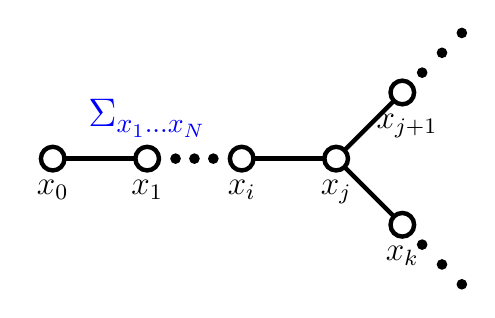
\begin{tikzpicture}[scale=0.6]
\draw [ultra thick] (-2,0) -- (0,0);
\draw [ultra thick, fill=white] (-2,0) circle [radius=0.25];
\node [below] at (-2,-0.25) {\large $x_{0}$};
\node [above, blue] at (0,0.25) {\Large $\Sigma_{x_1 \ldots x_N}$};
\draw [ultra thick, fill=white] (0,0) circle [radius=0.25];
\node [below] at (0, -0.25) {\large $x_1$};
\draw [fill] (0.6,0) circle [radius=0.1];
\draw [fill] (1,0) circle [radius=0.1];
\draw [fill] (1.4 ,0) circle [radius=0.1];
\draw [ultra thick] (2,0) -- (4,0);
\draw [ultra thick, fill=white] (2,0) circle [radius=0.25];
\node [below] at (2,-0.25) {\large $x_{i}$};
\draw [ultra thick] (4,0) -- (5.4,1.4);
\draw [ultra thick] (4,0) -- (5.4,-1.4);
\draw [ultra thick, fill=white] (4,0) circle [radius=0.25];
\node [below] at (4,-0.25) {\large $x_j$};
% \draw [fill] (4.6,0) circle [radius=0.1];
% \draw [fill] (5,0) circle [radius=0.1];
% \draw [fill] (5.4 ,0) circle [radius=0.1];
\draw [ultra thick,fill=white] (5.4,1.4) circle [radius=0.25];
\draw [fill] (5.82,1.82) circle [radius=0.1];
\draw [fill] (6.24,2.24) circle [radius=0.1];
\draw [fill] (6.66 ,2.66) circle [radius=0.1];
\node [below] at (5.5,1.15) {\large $x_{j+1}$};
\draw [ultra thick,fill=white] (5.4,-1.4) circle [radius=0.25];
\node [below] at (5.4,-1.65) {\large $x_k$};
\draw [fill] (5.82,-1.82) circle [radius=0.1];
\draw [fill] (6.24,-2.24) circle [radius=0.1];
\draw [fill] (6.66 ,-2.66) circle [radius=0.1];
\end{tikzpicture}}
%}
\sublabel{b}{
%\centerline{
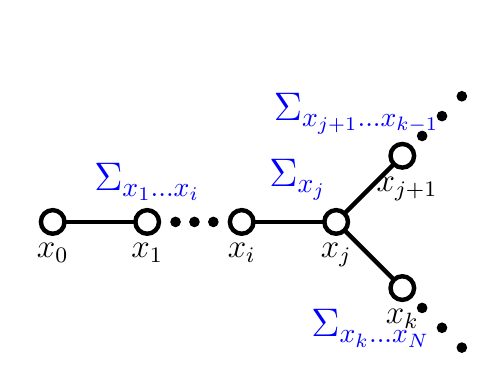
\begin{tikzpicture}[scale=0.6]
\draw [ultra thick] (-2,0) -- (0,0);
\draw [ultra thick, fill=white] (-2,0) circle [radius=0.25];
\node [below] at (-2,-0.25) {\large $x_{0}$};
\node [above, blue] at (0,0.25) {\Large $ \Sigma_{x_1 \ldots x_{i}}$};
\draw [ultra thick, fill=white] (0,0) circle [radius=0.25];
\node [below] at (0, -0.25) {\large $x_1$};
\draw [fill] (0.6,0) circle [radius=0.1];
\draw [fill] (1,0) circle [radius=0.1];
\draw [fill] (1.4 ,0) circle [radius=0.1];
\draw [ultra thick] (2,0) -- (4,0);
\draw [ultra thick, fill=white] (2,0) circle [radius=0.25];
\node [below] at (2,-0.25) {\large $x_{i}$};
\draw [ultra thick] (4,0) -- (5.4,1.4);
\draw [ultra thick] (4,0) -- (5.4,-1.4);
\draw [ultra thick, fill=white] (4,0) circle [radius=0.25];
\node [below] at (4,-0.25) {\large $x_j$};
\node [above left, blue] at (4, 0.25) {\Large $ \Sigma_{x_{j}}$};
\draw [ultra thick,fill=white] (5.4,1.4) circle [radius=0.25];
\draw [fill] (5.82,1.82) circle [radius=0.1];
\draw [fill] (6.24,2.24) circle [radius=0.1];
\draw [fill] (6.66 ,2.66) circle [radius=0.1];
% to add space between the figures
\draw [fill, white] (6.66,4) circle [radius=0.1];
\node [below] at (5.5,1.15) {\large $x_{j+1}$};
\node [above left, blue] at (6.4, 1.65) {\Large $ \Sigma_{x_{j+1} \ldots x_{k-1}}$};
\draw [ultra thick,fill=white] (5.4,-1.4) circle [radius=0.25];
\node [below] at (5.4,-1.65) {\large $x_k$};
\node [below left, blue] at (6.2, -1.65) {\Large $ \Sigma_{x_{k} \ldots x_{N}}$};
\draw [fill] (5.82,-1.82) circle [radius=0.1];
\draw [fill] (6.24,-2.24) circle [radius=0.1];
\draw [fill] (6.66 ,-2.66) circle [radius=0.1];
\end{tikzpicture}}
%}
}
\caption{Example motivating belief propagation update rule. (a)
  Marginalization of a graph with no loops.  (b) Shows how the partial sums at $x_j$ distribute over nodes.} 
\label{fig:bpmotivator2}
\end{figure}


To compute the message from node $j$ to node $i$:
\begin{enumerate}
\item Multiply together all messages (independent probabilities) coming in to node $j$, except for
 the message from node $i$ back to node $j$,
\item Multiply by the pairwise compatibility function $\psi_{ij}(x_i, x_j)$ (also independent of the other multiplicands).
\item Marginalize over the variable $x_j$.
\end{enumerate}
These steps are summarized in this equation to compute the message from node $j$ to node $i$:
\begin{equation} 
m_{ji}(x_i) = \sum_{x_j} \psi_{ij} (x_i, x_j) 
\prod_{k\in \eta(j) \mbox{\textbackslash}   i} m_{kj}(x_j)
\label{eq:bpupdate}
\end{equation} 
where $\eta(j) \mbox{\textbackslash}   i$ means ``the neighbors of
node $j$ except for node $i$.''  \Fig{\ref{fig:bpdiscrete}} shows this
equation in a graphical form.  Any local potential functions
$\phi_{j}(x_j)$ are treated as an additional message into node $j$, that is, $m_{0j}(x_j) = \phi_{j}(x_j)$.
For the case of continuous variables, the
sum over the states of $x_j$ in \eqn{\ref{eq:bpupdate}} is replaced by an integral over the
domain of $x_j$.

\begin{figure}
\centerline{
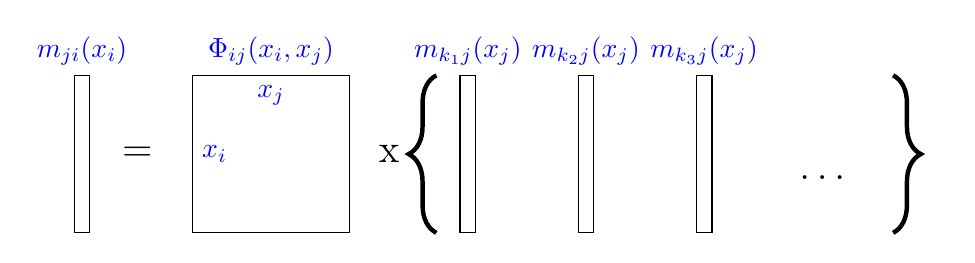
\begin{tikzpicture}
\draw [draw=black]  (-2.8, 2) rectangle (-3, 0);
\node [above, blue] at (-2.9, 2) {$m_{ji}(x_i)$};
\node at (-2.2,1) {\Large  $ =$};
\draw [draw=black]  (-1.5, 2) rectangle (0.5, 0);
\node [above,blue] at (-0.5, 2) {$\Phi_{ij}(x_i, x_j)$};
\node [below, blue] at (-0.5, 2) {$x_j$};
\node [right, blue] at (-1.5, 1) {$x_i$};
\node at (1.0,1) {\Large  $\mbox{x}$};
\draw [draw=black]  (1.9, 2) rectangle (2.1, 0);
\node [above, blue] at (2.0, 2) {$m_{{k_1}j}(x_j)$};
\node at (2.6,1) {\Large  $\hadamard$};
\draw [draw=black]  (3.4, 2) rectangle (3.6, 0);
\node [above, blue] at (3.5, 2) {$m_{{k_2}j}(x_j)$};
\node at (4.1,1) {\Large  $\hadamard$};
\draw [draw=black]  (4.9, 2) rectangle (5.1, 0);
\node [above, blue] at (5.0, 2) {$m_{{k_3}j}(x_j)$};
\node at (5.6,1) {\Large  $\hadamard$};
\node at (6.5,0.7) {\Large  $\ldots$};

% Adding large parentheses
\draw[decoration={brace, amplitude=10pt, mirror}, decorate, ultra thick] (1.6,2) -- node[right=12pt] {} (1.6,0);
\draw[decoration={brace, amplitude=10pt}, decorate, ultra thick] (7.4,2) -- node[right=12pt] {} (7.4,0);
\end{tikzpicture}}
\caption{Pictorial depiction of belief propagation message passing
 rules of \eqn{\ref{eq:bpupdate}}, where $\hadamard$ indicates elementwise multiplication (i.e., the Hadamard product).  
 % To send a message from node j to
%  node i:  We term-by-term multiply (shown by .*) the messages (column vectors)
%  coming in to node j, then matrix multiply (shown by $\mbox{x}$)
% the resulting column vector by the compatibility matrix $\Phi_{ij}(x_i, x_j)$ to obtain $m_{ji}(x_i)$.
} 
\label{fig:bpdiscrete}
\end{figure}


As mentioned previously, BP messages are partial sums in the
marginalization calculation.  The arguments of messages are always the
state of the node that the message is going to.
(BP follows the ``nosey neighbor rule'' (from Brendan Frey, Univ. Toronto): Every node is a house in some neighborhood. Your nosey neighbor says to you, ``Given what I've seen myself and everything I’ve heard from my neighbors, here’s what I think is going on inside
your house.'' (That metaphor especially makes sense if one has teenaged children.)


\subsection{Marginal Probability}

\begin{figure}
\centerline{\includegraphics[width=0.48\linewidth]{figures/graphical_models/bpi.pdf}} 
\caption{To compute the marginal probability at node $i$, we multiply
 together all the incoming messages at that node:  
$p_{i}(x_i) =  \prod_{j\in \eta(i)}  m_{ji}(x_i)$, including any local potential terms $\phi_i(x_i)$ as another message.
}
\label{fig:bpi}
\end{figure}
 
The marginal probability at a node $i$, \eqn{\ref{eq:discreteMarginalization}}, is the sum over the joint probabilities of all states except those of $x_i$.  Because we assume the network has no loops, the conditional
independence structure assures us that marginal probability at a node $i$ is the product of the sum of all states of all nodes in each
subtree connected to node $i$: Conditioned on node $i$, the probabilities within each subtree are independent. Thus the marginal probability at node $i$
is the product of all the incoming messages:
\begin{equation}
p_{i}(x_i) = \prod_{j\in \eta(i)}  m_{ji}(x_i)
\label{eq:bpmarginal}
\end{equation}
(We include the local clique potential at node $i$, $\psi_i(x_i)$, as
one of the messages in the product of all messages into node $i$).


\subsection{Message Update Sequence}
To find all the messages, how do we invoke the recursive BP update rule, \eqn{\ref{eq:bpupdate}}?  We can apply \eqn{\ref{eq:bpupdate}}
whenever all the incoming messages in the BP update rule are defined.  If there
 are no incoming messages to a node, then its outgoing message is
well-defined in the update rule.  This lets us start the recursive algorithm.

A node can send a message whenever all the incoming messages it needs
have been computed.  We can compute the outgoing messages
from leaf nodes in the graphical model tree, since they have no
incoming messages other than from the node to which they are sending a
message, which doesn't enter in the outgoing message computation.  Two
natural message passing protocols are consistent with that rule:
depth-first update, and parallel update.  In depth-first update, one
node is arbitrarily picked as the root.  Messages are then passed from
the leaves of the tree (leaves, relative to that root node) up to the
root, then back down to the leaves.  In parallel update, at each turn,
every node sends every outgoing message for which it has received all
the necessary incoming messages.  \Fig{\ref{fig:men}} depicts the
flow of messages for the parallel, synchronous update scheme and \Fig{\ref{fig:men2}} shows the flow for the same network, but with a depth-first update schedule.

Note that when computing marginals at many nodes, we reuse messages
with the BP algorithm.  A single message-passing sweep through all the
nodes lets us calculate the marginal at any node (using the
depth-first update rules to calculate the marginal at the root node).
A second sweep from the root node back to all the leaf nodes
calculates all the messages needed to find the marginal probability at
every node.  It takes only twice the number of computations to
calculate the incoming messages to every node, and thus the marginal probabilities everywhere, as it does to
calculate the incoming messages for the marginal probability at a single node.

\begin{figure}
\centerline{
\sublabel{a}{\includegraphics[width=0.20\linewidth]{figures/graphical_models/man1.pdf}}
\sublabel{b}{\includegraphics[width=0.20\linewidth]{figures/graphical_models/man2.pdf}}
\sublabel{c}{\includegraphics[width=0.20\linewidth]{figures/graphical_models/man3.pdf}}
}
\caption{{\bf Synchronous parallel update schedule} for BP message passing: Each node sends an outgoing message as soon as it receives the necessary incoming messages. Iterations: (a) one, (b) two, and (c) three.} 
\label{fig:men}
\end{figure}




\begin{figure}
\centerline{
\sublabel{a}{\includegraphics[width=0.20\linewidth]{figures/graphical_models/rootman1.pdf}}
\sublabel{b}{\includegraphics[width=0.20\linewidth]{figures/graphical_models/rootman2.pdf}}
\sublabel{c}{\includegraphics[width=0.20\linewidth]{figures/graphical_models/rootman3.pdf}}
\sublabel{d}{\includegraphics[width=0.20\linewidth]{figures/graphical_models/rootman4.pdf}}
}
\caption{
{\bf Depth-first BP message passing schedule}. Select a root node. (a) Start at leaves; (b) proceed to root; (c), perform an outgoing sweep; and (d) compute remaining messages, ending at leaf nodes.}
\label{fig:men2}
\end{figure}

\subsection{Example Belief Propagation Application: Stereo}

Assume that we want to compute the depth from a stereo image pair, such as the pair shown in figures~\ref{fig:canoe1}(a and b) and with their insets marked with the red rectangles, shown in figures~\ref{fig:canoe1}(c and d).   Assume that the two images have been rectified, as described in \chap{\ref{chap:stereo_vision}}, and consider the common scanline, marked in figures~\ref{fig:canoe1}(c and d) with a black horizontal line.  The luminance intensities of each scanline are plotted in figures~\ref{fig:canoe1}(e and f).  Most computer vision stereo algorithms \cite{Scharstein2002} examine multiple scanlines to compute the depth at every pixel, but to illustrate a simple example of belief propagation in vision, we will consider the stereo vision problem while considering only one scanline pair at a time.


\begin{figure}[t]
\centerline{
\sublabel{a}{\includegraphics[width=0.40\linewidth]{figures/graphical_models/lcanoebig.jpg}}
\sublabel{b}{\includegraphics[width=0.40\linewidth]{figures/graphical_models/rcanoebig.jpg}}
}
\centerline{
\sublabel{c}{\includegraphics[width=0.40\linewidth]{figures/graphical_models/lcanoe2.jpg}}
\sublabel{d}{\includegraphics[width=0.40\linewidth]{figures/graphical_models/rcanoe2.jpg}}}
% \centerline{
% \sublabel{e} {\includegraphics[width=0.30\linewidth]{figures/graphical_models/leftline.jpg}}
% \sublabel{f}{\includegraphics[width=0.30\linewidth]{figures/graphical_models/rightline.jpg}}}
\caption{(a) Left and (b) right camera images. (c and d): insets showing areas of analysis.}
\label{fig:canoe1}
\end{figure}

The graphical model that describes this stereo depth reconstruction for a single scanline is shown in \fig{\ref{fig:canoe3}}.  



\begin{figure}
\centerline{
\includegraphics[width=0.80\linewidth]{figures/graphical_models/stereomodel2.jpg}
}
\caption{Graphical model for the posterior probability for stereo disparity offset between the left and right camera views from a stereo rig.}
\label{fig:canoe3}
\end{figure}

Each unfilled circle in the graphical model (\fig{\ref{fig:canoe3}}) represents the unknown depth of each pixel in the scan line of one of the stereo images, in this example, the left camera image in \fig{\ref{fig:canoe1}}{c}.  The open circles mean that the depth of each pixels is an unobserved variable.  Often, we represent the depth as the {\bf disparity} between the left and right camera images, see \chap{\ref{chap:stereo_vision}}.


The intensity values of the left and right camera scan lines can be used to compute the local evidence for the disparity offset, $d[i, j]$, of each right camera pixel corresponding to the left image pixel at each right camera position, $[i,j]$.  For this example, we assume that each right camera pixel value, $\boldimg_r$ is that of a corresponding left camera value, $\boldimg_l$, but with independent, identically distributed (IID) Gaussian random noise added.  This leads to a simple formula for the local evidence, $\psi_i$, for the given depth value of any pixel,
\begin{equation}
    \psi_i = p(d[i,j] \given \boldimg_r, \boldimg_l) =  k \exp{\left( -\sum_{i=-10}^{i=10} \frac{(\boldimg_r[i,j] - \boldimg_l[i - d[i, j], j])^2}{2 \sigma^2}  \right)}
\end{equation}
For simplicity in this example, we discretize the disparity offsets into four different bins, each 45 disparity pixels wide.  We sum the local disparity evidence within each depth bin, then normalize the evidence at each position to maintain a probability distribution.  The resulting local evidence matrix, for each of the four depth states, at each left camera spatial position, is displayed in \fig{\ref{fig:canoe4}}{c}.  The intensities in each column in the third-row image add up to one.


\begin{figure}
\centerline{
\includegraphics[width=.8\linewidth]{figures/graphical_models/bpcanoes5.pdf}
}
\caption{
Belief propagation applied to graphical model, \fig{\ref{fig:canoe3}}, for the stereo problem. (a) Right and (b) left camera views. The black line shows the analyzed row. (c) Local evidence for each depth disparity at left camera. (d) Final rightward and (e) leftward belief propagation messages at each position. (f) Final marginalized posterior probability at each left camera pixel accurately finds the depth discontinuity.}
\label{fig:canoe4}
\end{figure}


The prior probability of any configuration of pixel disparity states is described by setting the compatibility matrices, $\mathbf{\phi}[s_i, s_{i+1}]$ of the Markov chain of \fig{\ref{fig:canoe3}}.  For this example, we use a compatibility matrix referred to as the Potts Model \cite{Wu1982}:
\begin{equation}
  \mathbf{\phi}[s_i, s_{i+1}] = 
    \begin{cases}
      1, & \text{if}\ s_i = s_{i+1} \\
      \delta, & \text{otherwise}
    \end{cases}
\end{equation}
For this example, we used $\delta = 0.001$

We then ran BP (equation [\ref{eq:bpupdate}]) in a depth-first update schedule.  For this network, that involves two linear sweeps over all the nodes of the chain, first from left to right, then from right to left.  Starting from the left-most node, we updated the rightward messages one node at a time, in a rightward sweep; then, starting from the right-most node, updated all the leftward messages one node at a time, in a leftward sweep.  The results are in \fig{\ref{fig:canoe4}}(d and e), respectively.

Once all the messages were computed, we used \eqn{\ref{eq:bpmarginal}} to find the posterior marginal probability at each node. That involves, at each position, multiplying together all the incoming messages, including the local evidence.  Thus, the values shown in \fig{\ref{fig:canoe4}}{f} are the product, at each position, of \fig{\ref{fig:canoe4}}{c, d and e}.
Note that for this scanline, in this image pair, there is a depth discontinuity at location of the red vertical mark in \fig{\ref{fig:canoe4}}, namely the canoe is closer to the camera than the ground beyond the canoe that appears to the right of the canoe.  The local evidence for depth disparity, \fig{\ref{fig:canoe4}}{c}, is rather noisy, but the marginal posterior probability, after aggregating evidence along the scanline, accurately finds the depth discontinuity at the canoe boundary.

\begin{comment}
\begin{figure}
\centerline{
\sublabel{a}{\includegraphics[width=0.80\linewidth]{figures/graphical_models/lcanoeline.jpg}}}
\centerline{
\sublabel{b}{\includegraphics[width=0.80\linewidth]{figures/graphical_models/rcanoeline.jpg}}
}
\caption{(a) and (b) show the luminance traces from the scanlines marked in black in Fig.~\ref{fig:canoe1}~(c) and (d), respectively.}
\label{fig:canoe2}
\end{figure}
\end{comment}



\section{Loopy Belief Propagation}

The BP message update rules only work to give the exact marginals when
the topology of the network is that of a tree or a chain.   In general, one can show that exact
computation of marginal probabilities for graphs with loops depends on
a graph-theoretic quantity known as the {\bf treewidth} of the graph \cite{Koller2009}.  For
many graphical models of interest in vision, such as 2D Markov random
fields related to images, these quantities can be intractably large.

%But the
Message update rules are described locally, and one might imagine that
it is a useful local operation to perform, even without the global
guarantees of ordinary BP.   It turns out that is true.   Here is the algorithm, also know as
{\bf loopy belief propagation algorithm}:
\begin{enumerate}
\item Convert graph to pairwise potentials.
\item Initialize all messages to all ones, or to random values
 between 0 and 1.
\item  Run the belief propagation update rules of
  \sect{\ref{sect:bpRules}} until convergence.
\end{enumerate}

One can show that, in networks with loops, fixed points of the
belief propagation algorithm (message configurations where the
messages don't change with a message update) correspond to minima of a
well-known approximation from the statistical physics community known 
as the Bethe free energy \cite{Yedidia00b}.  In practice, the solutions found by the loopy belief propagation algorithm can be quite good \cite{Murphy1999}.
%, and other algorithms in this vein have been developed which are better still \cite{Wainwright03}.


%% \section{MAP Estimation and Energy Models}

Instead of summing over the states of other nodes, we are sometimes
interested in finding the $\mathbf{x}$ that maximizes the joint probability.  The argmax
operator passes through constant variables just as the summation sign
did.  This leads to an alternate version of the BP
algorithm, \eqn{\ref{eq:bpupdate}}, with the summation (of multiplying the vector message products by the node compatibility matrix) replaced with argmax.  This is
called the {\bf max-product} 
\index{Max-product algorithm}
version of belief propagation, and it
computes an MAP estimate of the hidden states.   
Improvements have been developed over loopy belief propagation for the
case of MAP estimation; see, for example, tree-reweighted belief propagation \cite{Kolmogorov2006} and graph cuts \cite{Zabih2004}.


\subsection{Numerical Example of Belief Propagation}
\label{sect:numerical}

Here we work though a numerical example of belief propagation.  To make the arithmetic easy,
we'll solve for the marginal probabilities in the graphical model of
two-state (0 and 1) random variables shown in \fig{\ref{fig:numerical}}.


\begin{figure}
\centerline{\includegraphics[width=0.48\linewidth]{figures/graphical_models/numerical2.pdf}} 
\caption{Undirected graphical model used in belief propagation example.} 
\label{fig:numerical}
\end{figure}

That
graphical model has three hidden variables, and one variable observed to
be in state 0.  The compatibility matrices are given in the arrays
below (for which the state indices are 0, then 1, reading from left to
right and top to bottom):
\begin{equation}
\psi_{12}(x_1, x_2) = 
\begin{bmatrix}
1.0 & 0.9 \\
0.9 & 1.0 
\end{bmatrix}
\end{equation}

\begin{equation}
\psi_{23}(x_2, x_3) = 
\begin{bmatrix}
0.1 & 1.0 \\
1.0 & 0.1 
\end{bmatrix}
\end{equation}

\begin{equation}
\psi_{42}(x_2, y_2) = 
\begin{bmatrix}
1.0 & 0.1 \\
0.1 & 1.0 
\end{bmatrix}
\end{equation}

Note that in defining these potential functions, we haven't taken care to normalize the joint probability, so
we'll need to normalize each marginal probability at the end
(remember $p(x_1,
x_2, x_3, y_2) = \psi_{42}(x_2, y_2) \psi_{23}(x_2, x_3) \psi_{12}(x_1,
x_2)$, which should sum to 1 after summing over all states).


For this simple toy example, we can tell what results to expect by inspection, then verify that BP is doing the right thing.  Node $x_2$ wants very much to look like $y_2=0$, because
$\psi_{42}(x_2, y_2)$ contributes a large valued to the posterior
probability when $x_2 = y_2 = 1$ or when $x_2 = y_2 = 0$.  From
$\psi_{12}(x_1, x_2) $ we see that
$x_1$ has a very mild preference to
look like $x_2$.  So we expect the marginal probability at node $x_2$
will be heavily biased toward $x_2=0$, and that node $x_1$ will have a
mild preference for state 0.  $\psi_{23}(x_2, x_3)$ encourages 
$x_3$ to be the opposite of $x_2$, so it will be biased toward the state $x_3=1$.

Let's see what belief propagation gives.  We'll
follow the parallel, synchronous update scheme for calculating
all the messages.  The leaf nodes can send messages along their
edges without waiting for any messages to be updated.  For the message
from node 1, we have
\begin{eqnarray} 
m_{12}(x_2) & = & \sum_{x_1} \psi_{12} (x_1, x_2)  \nonumber \\
& = & 
\begin{bmatrix} 
1.0 & 0.9 \\ 
0.9 & 1.0 
\end{bmatrix}
\begin{bmatrix}
1 \\ 
1
\end{bmatrix}
% \\
%& = &
=
\begin{bmatrix}
1.9 \\ 
1.9
\end{bmatrix}
%\\
%&  = &
=
k_1
\begin{bmatrix}
1 \\ 
1
\end{bmatrix}
\end{eqnarray} 
For numerical stability, we typically normalize the computed messages in \eqn{\ref{eq:bpupdate}} so
the entries sum to 1, or so their maximum entry is 1, then remember
to renormalize the final marginal probabilities to sum to 1.
Here, we will normalize the messages for simplicity, absorbing the normalization into constants, $k_i$.

The message from node 3 to node 2 is
\begin{eqnarray}
m_{32}(x_2) & = & \sum_{x_3} \psi_{32} (x_2, x_3) \nonumber  \\
& = & 
\begin{bmatrix}
0.1 & 1.0 \\
1.0 & 0.1 
\end{bmatrix}
\begin{bmatrix}
1 \\ 
1
\end{bmatrix}
% \\
%& = &
=
\begin{bmatrix}
1.1 \\
1.1
\end{bmatrix}
%\\
%&  = &
=
k_2
\begin{bmatrix}
1 \\
1
\end{bmatrix}
\end{eqnarray}

We have a nontrivial message from observed node $y_2$ (node 4) to the hidden
variable $x_2$:
\begin{eqnarray}
m_{42}(x_2) & = & \sum_{x_4} \psi_{42} (x_2, y_2)  \nonumber \\
& = & 
\begin{bmatrix}
1.0 & 0.1 \\
0.1 & 1.0 
\end{bmatrix}
\begin{bmatrix}
1 \\
0
\end{bmatrix}
%\\
%& = &
=
\begin{bmatrix}
1.0 \\
0.1
\end{bmatrix}
\end{eqnarray}
where $y_2$ has been fixed to $y_2 = 0$, thus restricting $\psi_{42}
(x_2, y_2) $ to just the first column.

Now we just have two messages left to compute before we have all
messages computed (and therefore all node marginals computed from
simple combinations of those messages).  
The message from node 2 to node 1 uses the messages from nodes 4 to 2
and 3 to 2:
\begin{eqnarray}
m_{21}(x_1) & = & \sum_{x_2} \psi_{12} (x_1, x_2)  m_{42}(x_2) m_{32}(x_2) \nonumber \\
& = & 
\begin{bmatrix}
1.0 & 0.9 \\
0.9 & 1.0 
\end{bmatrix}
\left(
\begin{bmatrix}
1.0 \\
0.1
\end{bmatrix}
\hadamard
\begin{bmatrix}
1 \\
1
\end{bmatrix}
\right)
=
\begin{bmatrix}
1.09 \\
1.0
\end{bmatrix}
\end{eqnarray}

The final message is that from node 2 to node 3 (since $y_2$ is
observed, we don't need to compute the message from node 2 to node
4).  That message is:
\begin{eqnarray}
m_{23}(x_3) & = & \sum_{x_2} \psi_{23} (x_2, x_3)   m_{42}(x_2) m_{12}(x_2) \nonumber  \\
& = & 
\begin{bmatrix}
0.1 & 1.0 \\
1.0 & 0.1 
\end{bmatrix}
\left(
\begin{bmatrix}
1.0 \\
0.1
\end{bmatrix}
\hadamard
\begin{bmatrix}
1 \\
1
\end{bmatrix}
\right) 
=
\begin{bmatrix}
0.2 \\
1.01
\end{bmatrix}
\end{eqnarray}

Now that we've computed all the messages, let's look at the marginals
of the three hidden nodes.  The product of all the messages arriving
at node 1 is just the one message, $m_{21}(x_1)$, so we have
(introducing constant $k_3$ to normalize the product of messages to be a
probability distribution)
\begin{equation}
p_1(x_1) = k m_{21}(x_1) 
=
\frac{1}{2.09}
\begin{bmatrix}
1.09 \\
1.0
\end{bmatrix}
\end{equation}
As we knew it should, node 1 shows a slight preference for state 0.

The marginal at node 2 is proportional to the product of three messages.
Two of those are trivial messages, but we'll show them all for
completeness:
\begin{eqnarray}
p_2(x_2) & = & k_4 m_{12}(x_2)  m_{42}(x_2)  m_{32}(x_2) \\
& = & k_4 
\begin{bmatrix} 
1 \\ 
1
\end{bmatrix}
\hadamard
\begin{bmatrix}
1.0 \\
0.1
\end{bmatrix}
\hadamard
\begin{bmatrix}
1 \\ 
1
\end{bmatrix}
%\\
%& = &
=
\frac{1}{1.1}
\begin{bmatrix}
1.0 \\
0.1
\end{bmatrix}
\end{eqnarray}
As expected, belief propagation reveals a strong bias for node 2 being in state 0.

Finally, for the marginal probability at node 3, we have
\begin{equation}
p_3(x_3) = k_5 m_{23}(x_3) 
=
\frac{1}{1.21}
\begin{bmatrix}
0.2 \\
1.01
\end{bmatrix}
\end{equation}
As predicted, this variable is biased toward being in state 1.

By running belief propagation within this tree, we have computed the
exact marginal probabilities at each node, reusing the intermediate
sums across different marginalizations, and exploiting the structure
of the joint probability to perform the computation efficiently.  If
nothing were known about the joint probability structure, the
marginalization cost would grow exponentially with the number of nodes
in the network.  But if the graph structure corresponding to the joint
probability is known to be a chain or a tree, then the marginalization
cost only grows linearly with the number of nodes, and is quadratic in
the node state dimensions.  The belief propagation algorithm enables inference in many large-scale problems.

\section{Relationship of Probabilistic Graphical Models to Neural Networks}

The probabilistic graphical models (PGMs) we studied in this chapter and neural networks (NNs) share some characteristics, but are quite different.  Both share a graph structure, with nodes and edges, but the nodes and edges mean different things in each case.  Below is a brief summary of the differences:

\begin{itemize}
    \item {\bf Nodes}: The nodes of a NN diagram typically represent a real-valued scalar activations.  The nodes of a PGM represent a random variable, real or discrete-valued, and scalars or vectors.
    \item {\bf Edges}:  Edges in PGMs determine statistical dependencies.  Edges in NNs determine which are involved in a linear summation to the next layer.
    \item {\bf Computation}:  The big difference between PGMs and NNs lies in what they calculate.  PGMs represent factorized probability distributions and pass messages that allow for the computation of  probabilities, for example, the marginal probability at a node. In contrast, NNs compute results that minimize some expected loss or an energy function \cite{LeCun2006,LeCun2007}.  That different goal, that is, minimizing an expected loss rather than calculating a probability, allows for more general computations by a neural network at the cost of output that may be less modular or less interpretable because they are not probabilities.
\end{itemize}
Both PGMs and NNs can have nodes organized into grid-like structures but also more generally in arbitrary graphs; see, for example, \cite{Gilmer2017,Kipf2017}.

\section{Concluding Remarks}

Probabilistic graphical models provide a modular representation for complex joint probability distributions. Nodes can represent pixels, scenes, objects, or object parts, while the edges describe the conditional independence structure. For tree-like graphs, belief propagation delivers optimal inference. In general graphs with loops, it can give a reasonable approximation.
 % Bill
%% \include{chapters/bill/inference_in_graphical_models} % Bill
% 
%\setcounter{chapter}{42}
\chapter{How to Do Research\index{Research}}
\label{chapter:how_to_do_research}

\section{Introduction}

The jump from problem sets into research 
can be hard.  Sometimes we see students who ace their
classes but struggle with their research.  In little bites, here is what we think is important for succeeding in research as a graduate student.  This chapter is written as advice from research advisor to a graduate student (so we use use the first person in the text), but we hope that this advice will be useful for anyone learning how to create and debug research or engineering projects.

\section{Research Advice}

The first piece of advice can go on a bumper sticker: {\bf ``Slow down to speed up.''}   In
  classes, the world is rigged.  There's a simple correct answer and the problem is structured to let you come to that answer.  You get  feedback with the correct answer within a day after you submit  anything.

Research is different.  No one tells you the right answer, and we may not know if there is a right answer.  We don't know if something doesn't work because there's a  silly mistake in the program or because a broad set of assumptions is flawed.

How do you deal with that?  Take things slowly.  Verify your
assumptions.  Understand the thing, whatever it is---the program, the algorithm,  or the
proof.  As you do experiments, only change one thing at a time, so you know what the outcome of the experiment means.

It may feel like you're going slowly, but you'll be making much more progress than if you flail around, trying different things, but not understanding what's going on. \\

\begin{figure}[htpb!]
\centerline{\epsfig{file=figures/how_to_do_research/bumper.jpg,width=2.5in}}
\caption{Research advice for a bumper sticker.}
\label{fig:vw}
\end{figure}


%% http://bethpartin.com/denver-photos-vw-bus-on-capitol-hill/
\noindent {\bf Please don't tell me ``it doesn't work.''}  
  Of course, it doesn't work.  If there's a single mistake in the    chain, the whole thing won't work, and how could you possibly go  through all those steps without making a mistake somewhere?  What I want to   hear instead is something like, ``I've narrowed down the problem to   step B.  Until step A, you can see that it works, because you put in
  X  and you get Y out, as we expect.   You can see how it fails here
  at   B.  I've ruled out W and Z as the cause.'' \\
  
\noindent {\bf ``This sounds like hard work.''}  Yes.  It's no longer about being  smart.  By now, everyone around you is smart.  In graduate school,   it's the {\em  hard workers} who  pull ahead.  This happens  in sports, too.  You always read stories about how hard the great players work, being the first ones out to practice, the last ones to
  leave, and so on. \marginnote{A co-author, who generally works harder than I do, tells me I should add comments here about the importance of taking time off from work and maintaining a good life/work balance.  That is true: you should work at a pace you can sustain, and you should refresh yourself by making time for the things that matter more than work, such as relationships, service, and relaxation.  Perhaps the point is to protect your time so you will have enough time to do the research well.} \\
  
  
  
\noindent {\bf ``How do I get myself to work hard enough to do research
  well?''}  It all plays out if you love what you're doing.
  You become good at it because you spend time at it and you do that because you enjoy it.
  So pick something to work on that you can love.   If
  you're not the type who falls in love with a problem, then just know   that working hard is what you have to do to succeed at research. \\
  
\noindent {\bf The above isn't completely true.}  Beyond
  working hard, there's also {\em steering}.  We're like boats.  We need
  motors---that's the part about working hard.  But we also need a rudder for
  steering---that means stepping back periodically to make sure
  we're working on the right thing.  On the topic of steering,
  I find time management books to be very helpful.  They teach you how  to spend your time solving the right problems. \\
  
\noindent {\bf Toy models.}
There's a concept I want a
  simple phrase for, and maybe you can help me think up a good name.
  It's ``the simplest toy model that captures the main
  idea''  (TSTMTCTMI).    Anyway, simple toy models
 always help me.  With a good one, 
  you can build up intuition about what matters, which is a big
  advantage in research.  

Here's an example.  The color constancy problem is to estimate surface
reflectance colors when we only get to observe the
wavelength-by-wavelength product of the each surface
reflectance spectrum and the unknown
illuminant spectrum.  A toy model for that problem is to try to estimate the scalars
$a$ and $b$ from only observing their product, $y = a \times b$.  There's a
surprising richness even to this simple problem, and thinking about it
allows you to think through loss functions and other aspects of
Bayesian decision theory (\fig{\ref{fig:toy}}).  I co-authored a paper that discusses 
$y = a \times b$ for much of the manuscript \cite{Freeman95a}.
Another toy model is to consider,  as a proxy for complicated shaded surfaces, a
single bump.  You get the idea.
\begin{figure}[h]
\centerline{
\epsfig{file=figures/how_to_do_research/abproblem.eps,width=1.4in}}
\caption{A toy model for the color constancy problem:  $y = a \times b$. The plot shows the possible solutions for $a$ and $b$ when $y=1$.}
\label{fig:toy}
\end{figure}

Having the intuitions from working with toy problems gives you a big advantage in the research, because you can figure out what will work by thinking it through with your toy model. \\

\noindent {\bf Strategies for success.}  Here is a parable, as told by my friend Yair Weiss.  There is a weak
and a strong graduate student.  They are both asked by their advisor
to try a particular approach to solving a research problem.
The weak student does exactly what the advisor has asked.  But the advisor's
solution fails, and the student reports that failure.
The strong student starts doing what the advisor has asked, sees that
it doesn't work, looks around within some epsilon ball
of the original proposal to find what does work, and reports that solution.
\begin{figure}[htpb!]
\centerline{
\epsfig{file=figures/how_to_do_research/twoStudents.pdf,width=2in}}
\caption{The parable of the two students.}
\label{fig:students}
\end{figure}
%% http://www.123rf.com/photo_2851187_the-two-students-with-the-book.html

\noindent {\bf Sometimes it's useful to think that everyone else is completely off-track.}  This
  lets you do things that no one else is doing.  It's
  best not to be too vocal about that.  You can say something like,
  ``Oh, I just thought I'd try out this direction.'' \\
  
\noindent {\bf It's also sometimes useful to remember} that many smart people have
  worked on this and related problems and written their thoughts and results
  down in papers.  Don't be caught flat-footed with a large body of closely
  related literature that you aren't familiar with.  \\
  
\noindent {\bf How a business school might talk about your research}.   You have a brand:  you.  There are many impressions you want to build up about your brand:  that person always does great work, they have good
  ideas, they give great talks, they write wonderful software.
  Promote your brand.  Build up a great reputation for yourself by  consistently behaving in the way you'd like to be thought of.\\
% \begin{figure}[htpb!]
% \centerline{
% \epsfig{file=figures/how_to_do_research/applered.eps,width=0.6in}}
% \caption{Nurture your research brand.  }
% \label{fig:brand}
% \end{figure}
%% http://hms-somerset-co.blogspot.com/2012/12/apple-logo.html


\noindent {\bf Cultivate your strengths and play to those strengths.}  Some
  possible strengths include  being broad, being creative, being  a great implementer, or being great at doing theory.  \\
  
\noindent {\bf Please don't report to me and say, ``This instance doesn't work.''}  Why  doesn't it work?  Why should it work?   Is there a simpler case we  can make work?  Do you think it's a general issue that affects all
  problems of this category?  Can you think of what's  not working?  Can you contort things
 to make an example that does work?  At the very least, can you make it fail
 worse, so we understand some aspects of the system?  \\
 
\noindent {\bf Progress.} I love to hear about progress when I meet with students, but  note that  I have a very general notion of
 progress.  Progress can include things like ``I've shown why this doesn't work,'' ``I've
 simplified the task to get it to start working,'' or ``I spent the
 whole time reading because I know I have to understand this before I
 can make any progress.'' \\
 
\noindent {\bf Please don't hide from me.}  Let's talk.  I
  like it when you track me down and insist that we talk, for example,  if I've been traveling. \\
  

\noindent {\bf On collaboration.}  Science is generally a team sport.   What matters in a collaboration is whether the work is insightful,  foundational, or impactful.  It doesn't matter that many people were involved.
It is much better to be one of 10 contributors to a great paper than to be the sole author on an unimportant paper. The relationships formed through collaborations can become friendships that last over your career. \\

\noindent {\bf On authorship.}  What names should be on a paper? Everyone who contributed to the paper.  Contributions can be through experimentation, contributing a seminal idea that the paper builds on, or helping with the writing.  Sometimes an authorship contribution can include trying out a research direction that didn't work. If I'm on the fence about whether someone contributed enough to be an author, I usually ask the person themselves, and go with whichever outcome they prefer. 


\section{Concluding Remarks}  


For a presentation to the visiting admitted MIT computer science graduate students, I
  emailed all MIT Computer Science and Artificial Intelligence Laboratory (CSAIL) researchers and faculty members, asking ``Please send me   what you think is   the most important  quality for success in graduate school.''   I compiled their responses (along with photos of the responders) into slides that are available online:  
\begin{verbatim}
http://people.csail.mit.edu/billf/talks/10minFreeman2013.pdf
\end{verbatim}
I think it's a lot of good advice about research. 


\marginnote{{\bf One final note about doing research.}  We hope you love it.  We  certainly do.  The research community is a community of people who are passionate about what they do, and we welcome you to it!}









% 
%\setcounter{chapter}{43}
\chapter{How to Write Papers\index{Papers}}
\label{chapter:how_to_write_papers}

\section{Introduction}
An important part of research is communicating your results to others, so we include our thoughts about how to write good papers.  A video presentation of material related to this chapter is \cite{FreemanPapers2020}.

Many graduate students we know feel it is important to coauthor many papers.  While the number of papers a student has can be a rough measure of research productivity, it is our experience as mentors, faculty search committee members, and industrial research managers that {\em only the good papers count}. (We acknowledge that this is not true everywhere, and some institutions simply count papers. But you should still strive to make all your papers good!)  This emphasis is shown in \fig{\ref{fig:impact}}, a plot of made-up data that summarizes our impression, formed over many years, of the relationship between paper quality and its impact on one's career.  Only the really good papers matter for your career.  So it makes sense to learn how to write the best possible paper from any given piece of research work.

\begin{figure}
\centerline{
\includegraphics[width=0.60\linewidth]{figures/papers/impact.jpg}}
\caption{Plot of conjectured data showing the impact of a paper on one's career, as a function of paper quality. }
\label{fig:impact}
\end{figure}


\section{Organization}
The Ph.D. thesis advisor of two of us, Prof. Edward Adelson, wrote some good advice in response to a student's question of how to write a good paper \cite{Adelson92}:

\begin{itemize}
\item Start by stating which problem you are addressing, keeping the  
  audience in mind.  They must care about it, which means that sometimes 
  you must tell them why they should care about the problem. 
  
\item Then state briefly what the other solutions are to the problem, and why they aren't satisfactory.  If they were satisfactory, you wouldn't need to  do the work.  

\item Then explain your own solution, compare it with other solutions, and say why it's better.  

\item At the end, talk about related work where similar techniques and experiments have been used, but applied to a different problem.  
\end{itemize}

That structure fits well with a progression of section headings typical of  many conference papers.  As an example, here are the headings from paper \cite{Fergus2006}, coauthored by one of us.  The structure is useful for many research papers:

\begin{tabular}{ll}
1. & Introduction \\
2. & Related work \\
3. & Main idea \\
4. & Algorithm \\
& 4.1 Estimating the blur kernel \\
& \hspace{1cm} 4.1.1 Multiscale approach \\
& \hspace{1cm} 4.1.2 User supervision \\
& 4.2 Image reconstruction \\
5. & Experiments \\
& 5.1 Small blurs \\
& 5.2 Large blurs \\
& 5.3 Images with significant saturation \\
6. & Discussion \\
\end{tabular}





\subsection{The Paper's Introduction}
Regarding paper introductions, Kajiya \cite{Kajiya1993} writes,
``You must make your paper easy to read. You've got to make it easy for anyone to tell what your paper is about, what problem it solves, why the problem is interesting, what is really new in your paper (and what isn't), why it's so neat. And you must do it up front. In other words, you must write a dynamite introduction.''

\subsection{Main Idea}
When appropriate to the paper, it can be very helpful to show a simple example that captures the main idea of the paper.  Here is a figure from a different paper \cite{Simoncelli92} that conveys the main idea very simply.  The paper's main idea was that wavelets lacked important desirable features for an image representation.  \Fig{\ref{fig:wavelet}} shows the failure of a wavelet representation to form a  translation invariant representation.  The top row shows two versions of the same signal, differing only in a one-sample translation.  The bottom three rows show the coefficients of the high-, mid-, and low-frequency bands of a wavelet representation of that signal.  The figure points out in a simple way the drawback of a wavelet representation with aliased subbands that was the focus of the paper:  as the signal translates, the signal representation energy moves to different frequency bands and changes form within the mid-frequency band.


\begin{figure}
\centerline{
\includegraphics[width=0.65\linewidth]{figures/papers/wavelet2.pdf}}
\caption{Effect of translation on the wavelet representation of a signal  (caption and figure after \cite{Simoncelli92}).  (a) An input signal.  (b-d) The high-, mid-, and low-frequency coefficients within a wavelet subband decomposition.  (e) The same input signal, translated one sample to the right.  (f–h) The decomposition of the shifted signal into the same three bands.  Note the drastic change in the transform coefficients induced by the shift.}
\label{fig:wavelet}
\end{figure}


\subsection{Experimental Results}
In earlier days of computer vision research, good ideas could be presented with only plausibility arguments to support them.  However, 
modern standards require that assertions in a paper be backed up with experimental evidence.  Readers will be expecting a table quantitatively comparing the performance of your algorithm with that of the previous state-of-the-art.  If you are proposing a new task for which there aren't previous benchmarks, you should still compare with an algorithm that solves a related task, noting that the algorithm was designed for a different task.  

\begin{figure}
\centerline{
\includegraphics[width=0.75\linewidth]{figures/papers/resultTable.pdf}}
\caption{A prototypical table of results, from \cite{Owens2016}  Rows are different algorithms, or ablations of a favored algorithm. Columns are datasets or tasks, and the numbers indicate performance, with the best performances given in bold. }
\label{resultsTable}
\end{figure}


\subsection{How to End the Paper}

A cautionary note on how {\em not} to end the paper.  Conference papers are often written under deadline pressure, and there is inevitably a list of results that the authors wanted to obtain that have been left uncompleted.  You should resist the temptation to describe the items that were left unfinished in a section on ``Future Work.''  It is hard to imagine a weaker way to end the paper than to enumerate all the things the paper doesn't accomplish, providing a summary of where it falls short.

Instead, the paper can finish with a review what has been presented, emphasizing the contributions.  How has the world changed, now that the reader has read this paper?  What new research directions have been opened up;  what can we do now that we couldn't do before?

\section{General Writing Tips}

Donald Knuth, the author of the classic book series, \booktitle{The Art of Computer Programming}, wrote \cite{Knuth1989},``Perhaps the most important principle of good writing is to keep the reader uppermost in mind:  What does the reader know so far?  What does the reader expect next and why?''

Our mental image is that of a great host, who anticipates every need of their house guest: after you arrive, they say, ``Can I take your coat?  Would you like something to drink?''  At every moment, they know what you might be wanting and how to help you find it.

\subsection{Use Fewer Words}

In \booktitle{The Elements of Style} \cite{Strunk}, Strunk and White write, ``Vigorous writing is concise.  A sentence should contain no unnecessary words, a paragraph no unnecessary sentences, for the same reason that a drawing should have no unnecessary lines and a machine no unnecessary parts.''

To make this point in the context of scientific writing, the following is a paragraph that one of the authors of this textbook wrote with a student.  

\begin{quote}
The underlying assumption of this work is that the estimate of a given
node will only depend on nodes within a patch:  this is a locality
assumption imposed at the patch-level. This assumption can be
justified in case of skin images since a pixel in one corner of the
image is likely to have small effect on a different pixel far away
from itself.  Therefore, we can crop the image into smaller windows,
as shown in Figure 5, and compute the inverse J matrix of the cropped
window.  Since the cropped window is much smaller than the input
image, the inversion of J matrix is computationally cheaper.  Since we
are inferring on blocks of image patches (i.e., ignoring pixels outside
of the cropped window), the interpolated image will have blocky
artifacts.  Therefore, only part of xMAP is used to interpolate the
image, as shown in Figure 5.
\end{quote}
\marginnote{Original text: 149 words.}[0.5in]


While the text above conveys the desired technical information, it describes things in a roundabout way.  The word count is 149. Below, the paragraph has been rewritten to just 88 words without changing its meaning.

\begin{quote}
We assume local influence---that nodes only depend on other nodes
within a patch.  This condition often holds for skin images, which
have few long edges or structures.  We crop the image into small
windows, as shown in Fig. 5, and compute the inverse J matrix of each
small window.  This is much faster than computing the inverse J matrix
for the input image.  To avoid artifacts from the block processing,
only the center region of xMAP is used in the final image, as shown in
Fig. 5.
\end{quote}
\marginnote{Rewritten text conveying the same information: 88 words}[0.5in]

Note that writing more concise text helps your paper in two ways.  First, researchers are typically fighting against a page limit, particularly in conference submissions, so tighter text lets the author say more or add another figure.  Second, concise text is usually clearer and easier to understand.






\subsection{Title, Figure Captions, and Equations}
While we may imagine our reader reading every word of our paper, in our current era of many published papers, most of your readers will probably only skim your paper. We suspect that the engagement of readers with your paper will look something as shown in \fig{\ref{fig:engagement}}.

\begin{figure}
\centerline{
\includegraphics[width=0.50\linewidth]{figures/papers/readership.pdf}}
\caption{The conjectured readership of a computer science paper (conjectured relative amounts).  Many people will read the title, but far fewer will read the abstract or look at the figures.  Fewer still will read every word of the paper.  You should allow readers to access your paper at each level of engagement.}
\label{fig:engagement}
\end{figure}

If only because that is where most of your readership lies, you should write your paper so that readers will learn from it, even at those reduced levels of engagement.  The title should convey the top-level message of the paper.  The figures and their captions should be self-contained and tell the story of the paper.  The abstract should provide a good summary.

A good title can generate attention and interest for the paper.  ``What makes Paris look like Paris'' \cite{doersch2012what}
is a delightful paper, and the title lets the reader see that right away.  In contrast, one of us coauthored a paper called ``Shiftable Multi-scale Transforms.''  While that title is appropriate, it's not catchy.  After the paper was in print, we realized that we should have added the subtitle, ``What's wrong with wavelets?'' --- a catchy phrase that tells the main point of the paper.

Because you can assume that many of the readers of your figure captions will not be reading the full paper, {\em the captions should be self-contained}.  They should point out what readers are supposed to notice about the figure, to help both the full-paper reader and the figures-only reader. \Fig{\ref{fig:shapetime}} shows an example.

\begin{figure}
\centerline{
\includegraphics[width=0.55\linewidth]{figures/papers/shapetimeFig.jpg}}
\caption{Figure and caption from \cite{FreemanShapetime}. The caption should be understandable by itself, and should point to what the reader should take away from the figure. }
\label{fig:shapetime}
\end{figure}

Equations interposed with text can pose a challenge to the reader.  Does the reader stop to work through each equation, or continue reading as quickly as if the equation were words?  Knuth \cite{Knuth1989} and Mermin \cite{Mermin1989} both give advice on writing with equations.  Knuth writes,
``{\em Many readers will skim over formulas on their first reading of your exposition.  Therefore, your sentences should flow smoothly when all but the simplest formulas are replaced by `blah' or some other grunting noise.}''

Mermin adds,``{\em When referring to an equation identify it by a phrase as well as a number.  No compassionate and helpful person would herald the arrival of Eq. (7.38) by saying `inserting (2.47 and (3.51 into (5.13)...' when it is possible to say `inserting the form (2.47 of the electric field $E$ and the Lindhard form (3.51) of the dielectric function $\epsilon$ into the constitutive equation (5.13)...' }''


\subsection{Tone}

The tone of your writing is important.  You may feel pressure to oversell, hide drawbacks, and disparage others’ work.  It is in both your short-term and your long-term interest not to succumb to that pressure!  If your work has a shortcoming, it is much better that you point it out than to have someone else do so later.

Papers written from the point of view that ``we're all good researchers, doing our best'' are much more pleasant to read than papers written from the standpoint that everyone else is an idiot.  Note the delightful sentences written by Efros \cite{Efros01} when he was a graduate student, ``{\em A number of papers to be published this year, all developed independently, are closely related to our work.  The idea of texture transfer based on variations of [6] has been proposed by several authors (in particular, see the elegant paper by Hertzmann et al. in these proceedings).  Liang et al. propose a real-time patch-based texture synthesis method very similar to ours.  The reader is urged to review these works for a more complete picture of the field.}''  This generous tone wins over the reader and promotes long-lasting friendships with people who study the same problems you do.

You should develop a reputation for being clear and reliable.  Always convey an accurate impression of the performance of an algorithm.  If something doesn't work in important cases, let the readers know.  In \cite{Fergus2006}, we noted that our deblurring algorithm didn't work for a case where we had been sure it should work for a  maximum a posteriori (MAP)  estimation of the deblurred image. Some years later we learned, and described in \cite{Levin2011}, that we had been wrong to believe that MAP estimation of the deblurred image was feasible.  We were glad we had described our counterintuitive result years before.


\subsection{Author List}

The quality of the papers you write matters so much more than your positions within the author lists of the papers.  If adding more authors will make a paper better, then you should add more authors.   If a collaborator feels they should be an author, but you yourself are not sure, we find it is generally a good idea to trust the collaborator and to add them as a coauthor. It’s much better to be one of many authors on a great paper than to be one of just a few authors on a mediocre paper.

\subsection{Avoiding Rejection}

With the task of rejecting at least three-quarters of the submissions, conference area chairs, who make the acceptance decisions, are grasping for reasons to reject a paper.  Here’s a summary of reasons that are commonly used, and it is best not to provide the area chair with any of these easy reasons to reject your paper:

\begin{itemize}
\item Do the authors not deliver what they promise?
\item Are important references missing (and therefore one suspects the authors not up on the state of the art for this problem)?
\item Are the results too incremental (too similar to previous work)?
\item Are the results believable, with sufficient tests to support the claims?
\item Is the paper poorly written?  
\item Are there mistakes or incorrect statements?
\end{itemize}

As an area chair, the very good and the very bad papers are easy to deal with, and most of the decision-making effort goes to the borderline papers.  One of us writes, ``I find that much of my time is spent dealing with two kinds of borderline papers: cockroaches and  puppies with six toes.''  

``Cockroaches'' have no exciting contributions, but the reviews are ok and the results show incremental improvement to the state of the art.  They're hard to kill (hence the nickname), and maybe two-thirds are accepted as posters, and one-third are rejected.  As an author, it's best to work harder for the fresh results, to bring papers like this out of the cockroach category.

At the other end of the spectrum of borderline papers are ``puppies with six toes.''  These are delightful papers, but with an easy-to-see flaw.  The flaw may not matter (like six toes on a puppy) but makes the paper easy to reject, even though the paper may be fresh and wonderful.  Maybe two-thirds of those papers get rejected, and one-third maybe accepted as posters.  As an author, it may be better to wait for another submission cycle with a paper like this, to remove the easy to spot flaw.  Then the paper might receive an oral presentation at a subsequent conference submission cycle.

\begin{figure}
\centerline{
\sublabelnp{(a) Cockroach}{\includegraphics[width=0.23\linewidth]{figures/papers/cockroach.jpg}}
\sublabelnp{(b) Puppy with six toes}{\includegraphics[width=0.4\linewidth]{figures/papers/puppy6.jpg}}
}
\caption{Borderline papers from an area chair's perspective. (a) The cockroach represents a mundane, hard-to-reject paper with no glaring issues \cite{cockroach}. (b) The six-toed puppy represents delightful paper with some minor, easily spotted flaw, leading to potential rejection \cite{puppy}. }
\label{fig:areachair}
\end{figure}

\section{Concluding Remarks}
The approaches to writing and editing described previously all take time: 
 good writing involves lots of rewriting.  We find that the last days before a paper submission deadline are often better spent improving the structure, presentation, and clarity of the paper than in trying to obtain last-minute improvements to the results.

% %\setcounter{chapter}{44}
\chapter{How to Give Talks\index{Talks}}
\label{chapter:how_to_give_talks}

\section{Introduction}
Giving good talks is important for people who use the material of this book--for students, researchers, and engineers.
One  might think,  ``It is the work itself that really counts.  Giving a talk about it is secondary.''
But the ability to give a good talk is like having a big serve in tennis—by itself, it doesn’t win the game for you, but it sure helps.  And the very best tennis players all have great serves.  So we include in this chapter material that we have found helpful in giving talks.

There are many other sources for giving talks, and you should access several of them to pick out the tips that work best for you.  Prof. Patrick Winston's talk about giving talks is great \cite{WinstonSpeaks}, and another good source is this book \cite{Hoogterp}.   This chapter has heuristics that have worked well for us.

\subsection{A Taxonomy of Talks}

There are different kinds of talks.  Conference and workshop talks may range in length between 3 minutes for a ``fast-forward'' talk to 45 or 60 minutes for a keynote address.  You may be one of many speakers, sometimes speaking in different rooms at the same time.
Sometimes you will visit a university or company and speak in a special seminar. (Here \cite{MITFacultyJobTalks2022} is a list of tips regarding faculty job talks from the MIT faculty.)

It is very often the case that the audience will have a wide range of familiarity with the work and topic that you will present about.  In a small seminar to a competing research group, there may be many people who are very familiar with your work.  But even in such a small seminar, and especially to a larger group, there may be many people who don't know your area, nor perhaps not even your broad area.  So you will to include material to let the uninitiated not be lost.  Even people who are very  familiar with the topic will appreciate hearing material they already understand presented clearly and well.  

The tips in the chapter apply to talks of all lengths.  However, one class of talks is so short as to be a special case:  the very short talk.

\section{Very Short Talks (2 -- 10 minutes)}
Short talks are often advertisements, designed to persuade the listener to read your paper, or to listen to a longer version of the talk.  Rather than trying to convey many details about your work, you should aim to have the audience remember the main idea behind your work, and to share your excitement about the work.

For five minute talks describing students' final project class presentations, we suggest that the students cover these points:
\begin{enumerate}
\item What problem did you address?
\item Why is it interesting?
\item Why is it hard?
\item What was the key to your approach?
\item How well did it work?
\end{enumerate}
That structure can be used for other short talks, too.
For very short talks, the time needed to go through the whole thing is minimal, and there is no excuse not to practise the talk, from start to finish, several times.  Next, we cover points that we feel relate to all types of technical talks, regardless of length.


\section{Preparation}

\begin{figure}[htpb!]
\centerline{
\epsfig{file=figures/how_to_give_talks/speaker.jpg,width=3in}
}
\caption{The key to a good talk:  preparation and practice.}
\label{fig:speaker}
\end{figure}

\noindent We believe the keys to both a good talk and to overcoming nerves are the same: prepare and practice.  Think through your talk.  It's almost always better to give a talk from notes than to read it from a script--the audience feels  you're speaking to them so it's easier for them to pay attention.  But for people giving a talk in a language that they are not comfortable with, writing out a script ahead of time may be a better solution.  There may be parts of the talk that you feel are difficult to get through.  For those parts, even for a native speaker, it may help to write out what you plan to say.  When you give the talk, you may ignore the script, but having written it out once will make it easier to say.

Think through the talk and find the story--how one part relates to the next.  If you can't find that story, you may want to reorder the presentation to create a good story.

When you can, you should visit the room you'll be speaking in to identify any issues that may come up.  Will you be blocking anyone as you stand at the lectern to give the talk?  Will there be someone there to help you set up?  You should decide how to position yourself so that you can see your presentation, and also engage well with the audience.  


\section{Nervousness}

One of us writes, ``I used to be a nervous public speaker.  I still find the hours before giving a presentation to be stressful. I'm always reviewing my talk to try to improve it or to track down the answers to questions I think someone might ask me.  The more I prepare, and the better I know the lecture material, the less stressed I am."

A great cure for nervousness is to practice the talk aloud. Practice by yourself.  Practice in front of your friends.  

One approach \cite{Hoogterp} to calming  nervousness is to remind yourself, 
``Get over it.  They’re not there to see you, they’re there to hear the information.  Just convey the information to them.''

Some find this quote, attributed to Dr. Rob Gilbert \cite{Gilbert}, to be helpful:
``It's all right to have butterflies in your stomach. Your job is to get them to fly in formation.''

\section{Your Distracted Audience}
Before giving a talk, your mental image of the audience may be of many people, listening to your every word.  In reality, on most every speaking situation, your audience is a collection of people who are checking their social media or email, looking on their laptops for other talks to attend, or are hungry or fidgety.  How does one speak to such an audience?  We have to practise and prepare in order to engage the audience.



\section{Ways to Engage the Audience}
In the middle of Patrick Winston's talk about public speaking \cite{WinstonSpeaks}, he asks the audience the question, ``Can you think of a technique to get the audience more engaged in the talk?''  The answer, of course, is to ask them questions.

Bill Hoogterp \cite{Hoogterp} expands on that:  
``The audience is like a sheep dog, always wanting to be working.  Give the audience something to work on while they're listening to you. `Four' pushes people back, while `two plus two' draws them in."  You might pose a sub-problem to them that you had to address in your work, to get them thinking about how to solve that problem.  Then they'll be more receptive to hear your solution.

\subsection{Layer Your Talk}
It's often easier for the audience to listen to your talk if you layer it---provide verbal cues for new concepts and transitions between sections of the talk.  This helps even the attentive listener to follow the structure of your talk.  It keeps the distracted listener from being completely lost.  The distracted listener, only listening for the verbal headings of your talk, may hear,
``The probability of an observation has three terms to it.  $\ldots$ blah blah blah blah $\ldots$
So that gives us the objective function we want to optimize.  Now, how do we find the optimal value?  There are two approaches you can take.  $\ldots$ blah blah blah blah 
So now, with these tools in hand, we can apply this methods to real images. $\ldots$ blah blah blah blah $\ldots$"
Your verbal cues can help even a distracted listener follow your main points.

You can also make your talk easier to follow if you add verbal dynamics---variations in speed or intensity.  Find a part of the talk that is particularly special to you and let that show through.  One of us writes, "When I gave talks about image deblurring, I would emphasize one aspect that I particularly enjoy:
'I love this problem;  it’s beautifully underdetermined.  There are many ways we can explain a blurry image.  It could be that that’s what was there in the world--- we took a sharp picture of a world that happened to look blurry.  Or we took a blurred image of a sharp world.' " The audience loves to watch you be excited about something!


\subsection{People Like to See a Good Fight}

As described by Adelson \cite{Adelson95}, the audience loves to watch a good fight.  You can set up a fight between two competing conjectures.  For example, you might say, ``The flat earth theory predicts that ships will appear on the horizon as small versions of the complete ship.  Under that theory, you’d expect approaching ships to appear as in \fig{\ref{fig:boats}}{a}.  Conversely, the round earth theory predicts that the top of the sails will appear first, then gradually the rest of the ship below it, resulting in approaching ships looking as in \fig{\ref{fig:boats}}{b}.  The audience waits with anticipation as you show them the result from your experiment, \fig{\ref{fig:boats}}{c}, thus revealing the winning theory.

\begin{figure}[htpb!]
\centerline{
\sublabel{a}{\epsfig{file=figures/how_to_give_talks/boatsflat.jpg,width=1.5in}}
\sublabel{b}{\epsfig{file=figures/how_to_give_talks/boatsround.jpg,width=1.5in}}
\sublabel{c}{\epsfig{file=figures/how_to_give_talks/boatsphoto.jpg,width=1.5in}}
}
\caption{(a) The appearance of ships approaching a port, from the flat-earth theory.  (b) Their appearance as predicted by the round-earth theory.  (c) The experimental evidence:  a photograph of ships approaching a port \cite{mnsomero}. }
\label{fig:boats}
\end{figure}



\section{Show Yourself to the Audience}

In a lovely video, the actor Alan Alda describes the importance of  connecting with the audience in scientific presentations \cite{AlanAlda}.  Alda noted the improvement in scientific speaking of volunteers after they engaged in improvisational theater exercises.  After the exercises, the volunteers were primed to engage and connect with others, and their scientific talks sparkled.

Here's what we think an audience wants from a technical talk:
(a) To have one part follow from another and make sense.
(b) To learn a few things.
(c) To connect with the speaker, to share their excitement for the topic. They want to watch you love something!


\subsection{How to End the Talk}
How should you end your talk?  A common, but awkward, way is to end by asking, ``Are there any questions?''  The audience wants to clap at the end of a talk, but with that ending, they don't know whether to applaud or to ask a question, and they're likely to give only scattered applause \cite{Adelson95}.
Better is to close with ``Thank you.''  The audience then knows it's their time to applaud, and they will.  Then you can ask for questions.

We note that Patrick Winston disagrees with ending a talk with "thank you" \cite{WinstonSpeaks}.  He didn't like the implication that the audience was doing you some favor for attending your talk, and preferred to remind the audience of how he has kept his earlier promise to them regarding what they would learn after they listened to his talk.

\section{Concluding Remarks}
Prepare and practice your talks!  As you give the talk, let the audience see how much you enjoy what you've worked on.  Follow-up with the references in this chapter to find the collection of talk tips that works best for you.  Preparation and rehearsal are the best cures we know of for nervousness about giving a talk.



%% add the temporal aliasing figure and demo
% 
%% jan. 4, 2011  items to fix:
%% notation for math and reference to images.
%% how include eps figures.
%% make all the little figures (search for eps) in a common, nice matlab way for the
%% example filtering operations.

%\setcounter{chapter}{22}
\chapter{Temporal filters}
\label{chapter:temporal_filters}

%\section{Temporal convolutional filters}


Although adding time might seem like a trivial extension from 2D signals to 3D signals, and in many aspects it is, there are some properties of how the world behaves that make sequences to be different from arbitrary 3D signals. In 2D images most objects are bounded occupying compact and well defined image regions. However, in sequences, objects do not appear and disappear instantaneously unless they get occluded behind other objects or enter or exit the scene through doors or the image boundaries. So, the behavior of objects across time $t$ is very different than their behavior across space $n,m$. In time, objects move and deform defining continuous trajectories that have no beginning and never end.



\section{Modeling sequences}
\label{sect:modelingSequences}

Sequences will be represented as functions $f (x,y,t)$, where $x,y$ are the spatial coordinates and $t$ is time. As before, when processing sequences we will work with the discretized version that we will represent as $f \left[n,m,t \right]$, where $n,m$ are the pixel indices and $t$ is the frame number. Discrete sequences will be bounded in space and time, and can be stored as arrays of size $N \times M \times P$.


\begin{figure}
    \includegraphics[width=1\linewidth]{figures/temporal_filters/motion_illustration.eps}
    \caption{a) 8 Frames from a sequence with people walking. The frames are shown at regular time intervals. The full sequence had 90 frames (corresponding to 3 seconds of video). b) Space-time array, $f \left[n,m,t \right]$ of size $128 \times 128 \times 90$. c) Section for $m=50$, d) Section for $n=75$. Static objects appear as straight lines.}
    \label{fig:motion}
\end{figure}

Figure~\ref{fig:motion} illustrates this with one sequence shown in fig.~\ref{fig:motion}.a. This sequence has 90 frames and shows people on the street walking parallel to the camera plane and at different distances from the camera. Fig.~\ref{fig:motion}.b shows the space-time array $f \left[n,m,t \right]$. When we look at a picture we are a looking at a 2D section, $t=constant$, of this cube. But it is interesting to look at sections along other orientations.  Fig.~\ref{fig:motion}.c and d show sections for $m=constant$ and $n=constant$ respectively. Although they are also 2D images, their structure looks very different from the images we are used to seeing. Fig.~\ref{fig:motion}.c shows an horizontal section that is parallel to the direction of motion of the people walking. Here we see straight bands with different orientations. This bands appear to occlude each other. Each band corresponds to one person and its orientation is given by the speed of walk and the direction of motion. Fig.~\ref{fig:motion}.d looks like a foto-finish photograph as the ones used in sporting races. In both images (d) and (c), static objects appear as vertical stripes in (b), and horizontal stripes in (d).

One special sequence is when the image has a global motion with constant velocity $(v_x,v_y)$. In such a case we can write:
\begin{equation}
    f (x,y,t) = f_0 (x-v_xt,y-v_yt)
\end{equation}
where $f_0(x,y)= f (x,y,0)$ is the image being translated, and $v_x$ and $v_y$ are constants. We use continuous functions because it allows us to deal with any velocity values. This function assumes also that the brightness of the pixels does not change while the scene is moving ({\bf constant brightness assumption}).


In general, sequences will be more complex, but the properties of a globally moving image are helpful to understand local properties in sequences. We can also write models for more complex sequences. For instance, a sequence containing a moving object over an static background can be written as:
\begin{equation}
    f (x,y,t) = b(x,y) (1-m(x-v_xt,y-v_yt)) + o(x-v_xt,y-v_yt) m(x-v_x t,y-v_y t)
\end{equation}
where $b(x,y)$ is the static background image, $o(x,y)$ is the object image moving with speed $(v_x,v_y)$, and $m(x,y)$ is a binary mask that moves with the object and that models the fact that the object occludes the background.

\section{Modeling sequences in the Fourier domain}

The FT of a globally moving image is (using the shift property):
\begin{equation}
    F (w_x,w_y,w_t) = F_0 (w_x, w_y) \delta (w_t + v_x w_x + v_y w_y)
\end{equation}
The continuous FT of the sequence is equal to the product of the 2D FT of the static image $f_0(x,y)$ and a delta wall. To better understand this function let's look at a simple example on only one spatial dimension, as shown in figure~\ref{fig:mov_pulse_012}.

\begin{figure}
    \includegraphics[width=1\linewidth]{figures/temporal_filters/mov_pulse_012.eps}
    \caption{a) A sequence with one spatial dimension showing a static rectangular pulse. b) The rectangular pulse moves to the left at a speed $v=-0.5$ and c) moving towards the left, $v=-1$. As we work with discretized signals, speed units are in pixels per frame.}
    \label{fig:mov_pulse_012}
\end{figure}

Figure~\ref{fig:mov_pulse_012} shows the FT for a sequence with one spatial dimension, $f(x,t)$, that contains a blurry rectangular pulse moving at three different speeds towards the left. Fig.~\ref{fig:mov_pulse_012}.a shows a sequence when the pulse is static and fig.~\ref{fig:mov_pulse_012}.d shows its FT.  Across the spatial frequency $w_x$, the FT is approximately a sinc function. Across the temporal frequency $w_t$, as the signal is constant, its FT is a delta function.  Therefore the FT is a sinc function contained inside a delta wall in the line $w_t=0$. Fig.~\ref{fig:mov_pulse_012}.b shows the same rectangular pulse moving towards the left, $v_x=0.5$. Fig.~\ref{fig:mov_pulse_012}.e shows the sinc function but skewed a long the frequency line $w_t+0.5w_x=0$. Note that this is not a rotation of the sinc function from fig.~\ref{fig:mov_pulse_012}.d as the locations of the zeros lie at the same $w_x$ locations. Fig.~\ref{fig:mov_pulse_012}.c shows the pulse moving at a faster speed resulting in a larger skewing of its FT, Fig.~\ref{fig:mov_pulse_012}.f.


We let to the reader the work of computing its FT and visualizing the effect of the mask in the Fourier domain.



\section{Temporal filters}

Linear spatio-temporal filters can be written as spatio-temporal convolutions between the input sequence and a convolutional kernel (impulse response). Discrete spatiotemporal filters have an impulse response $h \left[n,m,t \right]$. The extension from 2D filter to spatio-temporal filters does not has any additional complications. We can also classify filters as low-pass, high-pass, etc. But in the case of time, there is another attribute used to characterize filters: causality.
\begin{itemize}
    \item Causal filters: these are filters with output variations that only depend of the past values of the input. This puts the following constraint: $h \left[n,m,t \right]=0$ for all $t<0$. This means that if the input is an impulse at $t=0$, the output will only have non-zero values for $t>0$. If this condition is satisfied, then the filter output will only depend on the input's past for all possible inputs.
    \item Non-causal filters: when the output has dependency on future inputs.
    \item Anti-causal filters: this is the opposite, when the output only depends on the future: $h \left[n,m,t \right]=0$ for all $t>0$.
\end{itemize}
Many filters are non-causal and have both causal and anti-causal components (e.g., a Gaussian filter). Note that non-causal filters can not be implemented in practice and, therefore, any filter with an anti-causal component will have to be approximated by a purely causal filter by bounding the temporal support and shifting in time the impulse response.

In this chapter, we have written all the filters as convolutions. However, some filters are better described as difference equations (this is specially important in time). An example of a difference equation is:
\begin{equation}
    g \left[n,m,t \right] = f \left[n,m,t \right] + \alpha \, h \left[n,m,t-1 \right]
\end{equation}
where the output $g$ at time $t$ depends on the input at time $t$ and the output at the previous time instant $t-1$ multiplied by a constant $\alpha$. We can easily evaluate the impulse response, $h \left[n,m,t \right]$, of such a filter by replacing $f\left[n,m,t \right]$ with an impulse, $\delta \left[n,m,t \right]$. The impulse response is:
\begin{equation}
    h \left[n,m,t \right] = \alpha^t  \delta \left[n,m \right] u \left[t \right]
\end{equation}
where $u\left[t \right]$, called the Heaviside step function, is:
\begin{equation}
    u \left[t \right] = \begin{cases}
        0 & \quad \text{if }  t <0  \\
        1 & \quad \text{otherwise } \\
    \end{cases}
\end{equation}
Most filters described by differences equations have an impulse response with infinite support. They are called IIR (Infinite Impulse Response) filters. IIR filters can be further classified as stable and unstable. Stable filters are the ones that given a bounded input, $| f \left[n,m,t \right] |<A$, produce a bounded output, $| g \left[n,m,t \right] | <B$. For this to happen, the impulse response has to be bounded. In unstable filters, the amplitude of the impulse response diverges to infinity. In the previous example, the filter is stable if and only if $| \alpha | < 1$.

Let's now describe some spatio-temporal filters.


\subsection{Temporal Gaussian}

As with the spatial case, we can define the same low-pass filters: the box filter, triangular filters, etc.  As an example, let's focus on the Gaussian filter. The spatio-temporal gaussian is trivial extension of the spatial gaussian filter we have seen in section~\ref{sec:spt_gaussian}:
\begin{equation}
    g(x,y,t; \sigma_x,\sigma_t) = \frac{1}{(2 \pi)^{3/2} \sigma_x^2\sigma_t} \exp{-\frac{x^2 +
            y^2}{2 \sigma_x^2}} \exp{-\frac{t^2}{2 \sigma_t^2}}
    \label{eq:gauss3dcont}
\end{equation}
Where $\sigma_x$ is the width of the gaussian along the two spatial dimensions, and $\sigma_t$ is the width on the temporal domain. As the units for $t$ and $x,y$ are unrelated, it does not make sense to set all the $\sigma$s to have the same value.

We can discretize the continuous gaussian by taking samples and building a 3D convolutional kernel. We can also use the binomial approximation. The 3D Gaussian is separable so it can be implemented efficiently as a convolutional cascade of 3 one dimensional kernels. Figure~\ref{fig:seq_filtered_kernel}.a shows a spatio-temporal gaussian. The temporal gaussian is a non-causal filter, therefore it is not physically realizable. This is not a problem when processing a video stored in memory. However, if we are processing an streamed video, we will have to bound and shift the filter to make it causal which will result in a delay in the output.

Figure~\ref{fig:sec_filtered_blur}.a shows one sequence and figure~\ref{fig:sec_filtered_blur}.b shows the sequence filtered with the gaussian from figure~\ref{fig:seq_filtered_kernel}.a.This Gaussian has a small spatial width, $\sigma=1$, and a large temporal width, $\sigma_t=4$ so the sequence is strongly blurred across time. The moving objects show motion blur and are strongly affected by the temporal blur, while the static background is only affected by the spatial width of the gaussian.

\begin{figure}
    \includegraphics[width=1\linewidth]{figures/temporal_filters/seq_filtered_kernel.eps}
    \caption{a) Spatio-temporal Gaussian with $\sigma=1$ and $\sigma_t=4$.  b) Same gaussian parameters but skewed by the velocity vector $v_x=-1, v_y=0$ pixels/frame, c) and $v_x=1, v_y=0$ pixel/frame.}
    \label{fig:seq_filtered_kernel}
\end{figure}

How could we create a filter that keeps sharp objects that move at some velocity $(v_x,v_y)$ while blurring the rest? Figure~\ref{fig:sec_filtered_blur}.c shows the desired output of such a filter. The bottom image shows one frame for a sequence filtered with a kernel that keeps sharp objects moving left at 1 pixel/frame while blurring the rest. This filter can be obtained by skewing the gaussian:
\begin{equation}
    g_{v_x,v_y}(x,y,t) = g(x - v_xt,y - v_yt, t)
\end{equation}
%where $g_{v_x,v_y}(x,y,t)$ is a skewed gaussian a long the space-time direction $(v_x,v_y,1)$. 
This directional blur is not a rotation of the original Gaussian as the change of variables is not unitary, but the same effect could be obtained with a rotation. Figure~\ref{fig:sec_filtered_blur}.c shows the effect when $v_x=-1, v_y=0$. The gaussian is shown in fig.~\ref{fig:seq_filtered_kernel}.b. The space-time section shows how the sequence is blurred everywhere except one oriented bad corresponding to the person walking left. Figure~\ref{fig:sec_filtered_blur}.d shows the effect when $v_x=1, v_y=0$. The output of this filter looks as if the camera was tracking one of the objects while the shutter was open, producing a blurry image of all the other objects.

\begin{figure}
    \includegraphics[width=1\linewidth]{figures/temporal_filters/seq_filtered_blur.eps}
    \caption{a) One frame from the input sequence and the space-time section (on top). b) Output when convolving the the gaussian from fig.~\ref{fig:seq_filtered_kernel}.a. c) Output of the convolution with fig.~\ref{fig:seq_filtered_kernel}.b, and d) output of the convolution with fig.~\ref{fig:seq_filtered_kernel}.c.}
    \label{fig:sec_filtered_blur}
\end{figure}


\subsection{Temporal derivatives}

Spatial derivatives were useful to find regions of image variation such as object boundaries. Temporal derivatives can be used to locate moving objects. We can approximate a temporal derivative for discrete signals as:
\begin{equation}
    f \left[m,n,t\right] - f \left[m,n,t-1\right]
\end{equation}

As in the spatial case, it is useful to compute temporal derivatives of spatio-temporal gaussians:
\begin{equation}
    \frac{\partial g}{\partial t} = \frac{-t}{\sigma_t^2} g(x,y,t)
\end{equation}
where $g(x,y,t)$ is the Gaussian as written in eq.~\ref{eq:gauss3dcont}. We can compute the spatio-temporal gradient of a gaussian:
\begin{equation}
    \nabla  g = \left( g_x(x,y,t), g_y(x,y,t), g_t(x,y,t) \right) =  \left(-x/\sigma^2, -y/\sigma^2, -t/\sigma_t^2 \right) g(x,y,t)
\end{equation}


What should we do if we want to remove only the objects moving at a particular velocity?

In the case of a moving image with velocity $(v_x, v_y)$, the sequence is $f (x,y,t) = f_0 (x-v_xt,y-v_yt)$, we can compute the temporal derivative of $f(x,y,t)$ as:
\begin{equation}
    \frac{\partial f}{\partial t} = \frac{\partial f_0}{\partial t} = -v_x \frac{\partial f_0}{\partial x} - v_y \frac{\partial f_0}{\partial y}
    \label{eq:brightnessconstancy}
\end{equation}

\begin{figure}
    \includegraphics[width=1\linewidth]{figures/temporal_filters/gaussians_xyt_seq.eps}
    \caption{Visualization of the space-time Gaussian. The gaussian has a width of $\sigma^2=\sigma_t^2=1.5$, and has been discretized as a 3D array of size $7 \times 7 \times 7$. Each image shows one frame. a)  Gaussian b) The partial derivative of the Gaussian with respect to $t$. c) Derivative along $v=(1,0)$ pixels/frame. d) $v=(-1,0)$ pixels/frame.}
    \label{fig:gaussian_seq}
\end{figure}

\begin{figure}
    \includegraphics[width=1\linewidth]{figures/temporal_filters/gaussians_xyt_section.eps}
    \caption{Spatio-temporal Gaussian $g\left[ n,t \right]$ and derivatives. a) Gaussian with $\sigma^2=1.5$. b) Partial derivative with respect to $t$. c) Partial derivative along $(1,-1)$, d) Partial derivative along $(1,1)$.}
    \label{fig:gaussian_xyt_section}
\end{figure}

If we compute the gradient of the gaussian along the vector $\left[1,v_x,v_y\right]$:
\begin{equation}
    h(x,y,t;v_x,v_y) = g_t+v_xg_x+v_yg_y = \nabla  g \left( 1,v_x,v_y \right)^T
\end{equation}
and we convolve it with $f_0 (x-v_xt,y-v_yt)$ we get a zero output (using eq.~\ref{eq:brightnessconstancy}):
\begin{eqnarray}
    f_0 (x-v_xt,y-v_yt) \circ h &=& f_0 (x-v_xt,y-v_yt) \circ \left(  g_t+v_xg_x+v_yg_y \right) \\
    &=& \left( \frac{\partial f_0}{\partial t} + v_x \frac{\partial f_0}{\partial x} + v_y \frac{\partial f_0}{\partial y} \right) \circ g \\
    &=& 0
\end{eqnarray}
The filter $h$ is shown in figure \ref{fig:gaussian_seq} as a sequence for different velocities. In the example shown in the figure, the gaussian (fig.~\ref{fig:gaussian_seq}.a) has a width of $\sigma^2=\sigma_t^2=1.5$, and has been discretized as a 3D array of size $7 \times 7 \times 7$. Figures b,c and d  show the filter $h$ for different velocities: $(v_x,v_y) =$ $(0,0)$, $(1,0)$ and $(-1,0)$. Fig.~\ref{fig:gaussian_xyt_section} shows the corresponding space-time sections of the same spatio-temporal gaussian derivatives. Both visualizations are equivalent and help to understand how the filter works.
%
%This is because we are computing spatio-temporal derivatives a long the direction of motion, so any object moving at that particular speed will be a constant a long that direction and its derivative will be zero. Fig.~\ref{fig:gaussian_xyt_section} shows a discrete spatio-temporal gaussian and temporal derivatives. Fig.~\ref{fig:gaussian_xyt_section}.a shows the gaussian across one spatial dimension and time. Fig.~\ref{fig:gaussian_xyt_section}.b is the temporal derivative, Fig.~\ref{fig:gaussian_xyt_section}.c shows the discretized gaussian gradient $g_t \left[n,t \right]+v_x g_x \left[ n,t \right]$ with $v_x=-1$ and Fig.~\ref{fig:gaussian_xyt_section}.d with $v_x=1$.


Such a filter will cancel any objects moving at the velocity $(v_x,v_y)$. By using different filters, each one computing derivatives a long different space-time orientations, we



\begin{figure}
    \includegraphics[width=1\linewidth]{figures/temporal_filters/seq_filtered_der.eps}
    \caption{a) Input sequence. b) $v_x=v_y=0$, c) $v_x=1$ pixels/frame. d) $v_x=-1$ pixel/frame.}
    \label{fig:tunedfilter}
\end{figure}


%\subsubsection{Motion detectors}
%
%Reighart model of the fly visual system?
%
%Maybe this is better later because it uses a battery of filters.


%FIGURE: velocity tunning? Compute the energy of the output as a function of the input velocity. This shows that fr large velocities the tunning is not tight. 



\subsection{Spatiotemporal Gabor filters}

\begin{figure}
    \centerline{
        \includegraphics[width=1\linewidth]{figures/temporal_filters/gabor_spacetime_FT.eps}
    }
    \caption{Space-time Gabor filters. a) Cosine and sine $x$-$t$ Gabor filter, and b) the sketch of its transfer function. c) Sketch of the transfer function of a spatiotemporal Gabor filter in 2 spatial dimensions ($x$-$y$-$t$).}
    \label{fig:spacetimefilts}
\end{figure}


Just as we did with Gaussian derivatives, extending Gabor filter for motion analysis is a direct generalization of the x-y 2D Gabor function to a x-y-t 3D Gabor function. Figure~\ref{fig:spacetimefilts}.a shows a x-t (cosine and sine) Gabor function in 1 spatial dimension, and  Figure~\ref{fig:spacetimefilts}.b shows a sketch of its Fourier transform. This function is selective to signals translating to the right with a speed $v=1$, i.e. $f(x-t)$. The red line in Figure~\ref{fig:spacetimefilts}.b shows Dirac line that contains the energy of the moving signal.

In 2 spatial dimensions, Figure~\ref{fig:spacetimefilts}.c shows the sketch of the Gabor transfer function. Note that the x-y-t Gabor filter is not selective to velocity. If we have a 2D moving signal $f(x-v_xt, y-v_yt)$, the Fourier transform is contained inside a Dirac plane. Therefore, there are an infinite number of planes that will pass by the frequencies of the Gabor filter. All those planes intersect the red line shown in Figure~\ref{fig:spacetimefilts}.c. A single Gabor filter can not disambiguate the input velocity.

Equation of the velocity as a function of the frequency tuning.


\section{Velocity-tuned filters}
\label{sect:velocityTunedFilters}

How can we measure input velocity? There are many different approaches in the computer vision community
for measuring motion.  Here we show that it is possible
to measure motion even with the simple processing machinery that
we've developed so far.

\begin{figure}
    \centerline{
        \includegraphics[width=1\linewidth]{figures/temporal_filters/gabor_spacetime_tiles.eps}
    }
    \caption{a) Space-time Gabor filters tiles. b) Set of Gabor filters selective to a particular velocity.}
    \label{fig:spacetimetiles}
\end{figure}



We can use quadrature pairs of oriented filters in space-time to find motion
speed and direction in the video signal.  We just need to find the
space-time orientation of strongest response. Figure \ref{fig:spacetimefilts}.a shows a set of Gabor filters sampling the space-time frequency domain. When the input contains a moving signal, we can use a set of filters to identify the plane in the Fourier domain that contains the input energy. Figure \ref{fig:spacetimefilts}.b shows the subset of filters that have the strongest output for a particular input motion.


As an illustration, Figure~\ref{fig:MT_velocity_tuned} shows one possible architecture to create velocity-selective units. The first layer is composed by Gabor filters (cosine and sine) which are frequency-selective units. The outputs are combined according to different planes in the Fourier domain to create velocity-selective outputs.

Given an input sequence, one can estimate velocity by looking at the velocity-tuned unit with the strongest response.

\begin{figure}
    \centerline{
        \includegraphics[width=1\linewidth]{figures/temporal_filters/MT_velocity_tuned.eps}
    }
    \caption{Architecture to create velocity-selective units. The first layer is composed by space-time Gabor filters (cosine and sine) which are frequency-selective units. Here we represent the impulse response of each filter by a small x-y-t cube. For each quadrature pair we compute the amplitude. Then amplitude outputs are combined according to form different planes in the Fourier domain to create velocity-selective outputs. A normalization layer can be added to normalize the outputs by dividing every output by the sum of all the amplitudes (not shown). The full architecture is non-linear.}
    \label{fig:MT_velocity_tuned}
\end{figure}

\section{Human Motion Processing}
\reviewcomment{Figures need reformatting.}

While researchers aren't sure of the precise computations involved in human motion processing, some experiments  can distinguish between classes of algorithms that the visual system may use.  The methods of the previous section are based on {\em spatio-temporal filtering} \cite{Adelson85}.  A second class of motion algorithms includes correlation-based methods, and can be called {\em pattern matching methods} \cite{Adelson85}.  In such methods, the motion offset of a spatial pattern from some starting position is computed by finding the position of highest correlation with the spatial pattern.

Adelson and Bergen proposed a beautiful motion illusion that distinguishes between two classes of motion algorithms that might be used by the visual system.  The illusion involves temporal filtering, motion processing, and aliasing and so provides a good review of the material in this chapter.

The illusion is presented in the video in Fig.~\ref{fig:blends}. The signals, and magnitudes of their space-time Fourier transforms, are developed in Figs.~\ref{fig:motionIllusion1} and \ref{fig:motionIllusion2}, building-up from simpler signals.  The three rows of Fig.~\ref{fig:motionIllusion1} show a stationary sinusoid, a moving sinusoid, and a moving square-wave.  The spatio-temporal Fourier transform of the stationary sinusoid, $I(x) = \cos(\pi \omega x)$ is $\delta(\nu) (\delta(\omega) + \delta(-\omega))$.  We have added a constant bias to the sinusoid to avoid negative intensity values, leading to an impulse at the center of the Fourier transform figure, Fig.~\ref{fig:motionIllusion1}~(c).  The resulting 3 colinear impulses are along the temporal frequency, $\nu = 0$ line.  A space-time plot of the signal, Fig.~\ref{fig:motionIllusion1}~(b), shows only vertical structures, indicating no motion.

A moving sinusoid has a similar Fourier transform magnitude, Fig.~\ref{fig:motionIllusion1}~(f), but with the spatio-temporal energies along a line perpendicular to the moving structures in the spatio-temporal signal, Fig.~\ref{fig:motionIllusion1}~(e).  A moving square wave is similar, but the extra harmonics needed to construct the square wave visible in the Fourier transform, Fig.~\ref{fig:motionIllusion1}~(i).

Continuing the development of the illusion, Fig.~\ref{fig:motionIllusion2}~(c) shows the Fourier transform and space-time plot of a square-wave moving in 1/4 period jumps each time increment.  This signal can be formed from Fig.~\ref{fig:motionIllusion1}~(h) by applying a periodic sample-and-hold function, resulting in the spectrum of  Fig.~\ref{fig:motionIllusion1}~(i) replicated over temporal frequencies, and multiplied by a sinc function over temporal frequency.  The resulting Fourier transform magnitude is shown in Fig.~\ref{fig:motionIllusion2}~(c).

Because orientation in space-time tells motion direction, Sect.~\ref{sect:modelingSequences}, the space-time plot of Fig.~\ref{fig:motionIllusion2}~(b) shows that the motion should be perceived to left.  This will be consistent with the behavior of velocity tuned filters, Sect.~\ref{sect:velocityTunedFilters}, responding to the lowest spatio-temporal frequency impulses shown in
Fig.~\ref{fig:motionIllusion2}~(c). However, if we remove the lowest spatial frequency sinusoid from the signal, the result is shown in
Fig.~\ref{fig:motionIllusion2}~(e), with spatio-temporal Fourier transform Fig.~\ref{fig:motionIllusion2}~(g).  Now the lowest spatio-temporal frequency cosine wave is oriented in the other direction.  This opposite slope is also visible in the spatial domain, in the space-time plot of Fig.~\ref{fig:motionIllusion2}~(e), and especially if we low-pass filter that, resulting in Fig.~\ref{fig:motionIllusion2}~(f).

The signal of the second row of Fig.~\ref{fig:motionIllusion2} poses a conundrum.  It can be argued that the signal moves to the left, just as does the signal of row 1 of Fig.~\ref{fig:motionIllusion2}.  The pattern match--the minimum correlation signal--indeeds move to the left.  But vision system examining the orientation of the lowest spatio-temporal frequency components of the signal in Fig.~\ref{fig:motionIllusion2}~(g), or looking at the dominant orientations in the space-time plots of
Fig.~\ref{fig:motionIllusion2}~(e) and (g), would find a signal moving to the right.

How does the signal appear to move to you?  We invite you to play the videos of Fig.~\ref{fig:motionIllusion2}~(c) and (g) (set your player to loop the videos) to assess which way each of the signals of  Fig.~\ref{fig:motionIllusion2} moves.   Fig.~\ref{fig:blends} show slow and fast motion versions of a blended signal, where the top half contains the lowest sinusoidal spatial frequency component of the square wave and the bottom half does not.  By moving your eye vertically, you can convince yourself that the entire pattern is moving rigidly to the left, yet it also appears that the top half is moving to the left and the bottom half is moving to the right.  This demonstration gives evidence for spatio-temporal filter-based motion processing within the human visual system, since such filtering would predict leftward motion for the top halves of the videos in Fig.~\ref{fig:blends}, and rightward motion for the bottom halves of those videos.

\begin{figure}
    \centerline{
        \hspace{-0.2in}
        \sublabelnp{(a)
            \href{https://groups.csail.mit.edu/vision/cvbook/videos/stillsineLoop.mov}{stationary sine wave (click for video)}}
        {
            \href{https://groups.csail.mit.edu/vision/cvbook/videos/stillsineLoop.mov}{\includegraphics[width=0.2\linewidth]{figures/temporal_filters/movie1.jpg}}}
        \sublabelnp{(b) space-time image}{\includegraphics[width=0.3\linewidth]{figures/temporal_filters/st1a.jpg}}
        \sublabelnp{(c) space-time Fourier transform}{\includegraphics[width=0.3\linewidth]{figures/temporal_filters/stdft1.jpg}}}
    \centerline{
        \sublabelnp{(d)
            \href{https://groups.csail.mit.edu/vision/cvbook/videos/movingSineLoop.mov}{moving sine wave (click for video)}
        }
        {
            \href{https://groups.csail.mit.edu/vision/cvbook/videos/movingSineLoop.mov}{\includegraphics[width=0.2\linewidth]{figures/temporal_filters/movie2.jpg}}}
        \hspace{0.1in}
        \sublabelnp{(e) space-time image}{\includegraphics[width=0.3\linewidth]{figures/temporal_filters/st2.jpg}}
        \hspace{0.5}
        \sublabelnp{(f) space-time Fourier transform}{\includegraphics[width=0.3\linewidth]{figures/temporal_filters/stdft2.jpg}}
    }
    \centerline{
        \sublabelnp{(g)
            \href{https://groups.csail.mit.edu/vision/cvbook/videos/movingSquareLoop.mov}{moving square wave (click for video)}
        }
        {
            \href{https://groups.csail.mit.edu/vision/cvbook/videos/movingSquareLoop.mov}{\includegraphics[width=0.2\linewidth]{figures/temporal_filters/movie3.jpg}}}
        \hspace{-0.8}
        \sublabelnp{(h) space-time Fourier transform}{\includegraphics[width=0.3\linewidth]{figures/temporal_filters/st3.jpg}}
        \hspace{-0.1in}
        \sublabelnp{(i) space-time Fourier transform}{\includegraphics[width=0.3\linewidth]{figures/temporal_filters/stdft3.jpg}}
    }
    \caption{Space-time signals, building toward the fluted square-wave motion illusion.    First row: stationary sine wave, (a) Movie of a motionless sine wave. (b) The space-time plot shows only vertical structure.
        (c) spatio-temporal Fourier transform has all energy on the zero temporal frequency axis, since nothing is moving.
        Second row:  (d) moving sine wave. (e) In the space-time plot, speed corresponds to local orientation. (f) The Fourier transform energy is sheared according to the sine wave's speed.
        Third row:  Moving square wave.  The additional harmonics required to form a square wave are visible in the spatio-temporal Fourier transform, (i).  }
    \label{fig:motionIllusion1}
\end{figure}

\begin{figure}
    \centerline{
        \sublabelnp{(a)
            \href{https://groups.csail.mit.edu/vision/cvbook/videos/steppedSquareLoop.mov}{stepped square wave (click for video)}
        }
        {
            \href{https://groups.csail.mit.edu/vision/cvbook/videos/steppedSquareLoop.mov}{\includegraphics[width=0.2\linewidth]{figures/temporal_filters/movie4.jpg}}}
        \sublabelnp{(b) space-time image}{\includegraphics[width=0.3\linewidth]{figures/temporal_filters/st4.jpg}}
        \sublabelnp{(c) space-time Fourier transform}{\includegraphics[width=0.3\linewidth]{figures/temporal_filters/stdft4.jpg}}
    }
    \centerline{
        \hspace{-0.6in}
        \sublabelnp{(d)
            \href{https://groups.csail.mit.edu/vision/cvbook/videos/steppedFlutedSquareLoop.mov}{fluted square wave  (click for video)}
        }
        {
            \href{https://groups.csail.mit.edu/vision/cvbook/videos/steppedFlutedSquareLoop.mov}{\includegraphics[width=0.2\linewidth]{figures/temporal_filters/movie5.jpg}}}
        \hspace{-0.6in}
        \sublabelnp{(e) space-time image}{\includegraphics[width=0.27\linewidth]{figures/temporal_filters/st5.jpg}}
        \hspace{-0.2in}
        \sublabelnp{(f) space-time Fourier transform}{\includegraphics[width=0.3\linewidth]{figures/temporal_filters/st6.jpg}}
        \hspace{-0.4in}
        \sublabelnp{(g) space-time Fourier transform}{\includegraphics[width=0.3\linewidth]{figures/temporal_filters/stdft5.jpg}}
    }
    \caption{Derivation of the fluted square-wave motion illusion, continued from Fig.~\ref{fig:motionIllusion1}.  First row:  This square wave moves in 1/4 wavelength jumps, instead of continuously.  This staggered motion generates the additional spatio-temporal frequencies shown in (a).  The lowest spatio-temporal frequency still indicates motion to the left.  Second row:  If we remove the lowest spatial frequency sine wave of the square wave, creating a "fluted square wave", then the lowest spatio-temporal frequency now moves in the other direction.  This is also visible from the space time plot in (e), and especially in the spatio-temporally low-pass filtered version, (f).}
    \label{fig:motionIllusion2}
\end{figure}



\begin{figure}
    \centerline{
        \sublabelnp{(a)
            \href{https://groups.csail.mit.edu/vision/cvbook/videos/blendedSlowLoop.mov}{motion illusion, slow (click for video)}
        }
        {
            \href{https://groups.csail.mit.edu/vision/cvbook/videos/blendedSlowLoop.mov}{\includegraphics[width=0.2\linewidth]{figures/temporal_filters/blendFrame.jpg}}}
        \sublabelnp{(b)
            \href{https://groups.csail.mit.edu/vision/cvbook/videos/fastBlendLoop.mov}{motion illusion, fast (click for video)}
        }
        {
            \href{https://groups.csail.mit.edu/vision/cvbook/videos/fastBlendLoop.mov}{\includegraphics[width=0.2\linewidth]{figures/temporal_filters/blendFrame.jpg}}}
    }
    \caption{"Impossible combination" of ordinary and  fluted square-waves (view on looping display).  While one can verify, by tracing a finger or scanning your eyes, that the entire structure is moving rigidly to the left, the bottom half appears to be moving to the right.  At a fast speed, (b), the effect is accentuated.}
    \label{fig:blends}
\end{figure}



%Here's a mock-up of a real scene.  We have a stationary background,
%and two cars driving in opposite directions.  (Thanks to Anat Levin
%for creating this slide).
%
%
%\begin{figure}
%\centerline{
%\includegraphics[width=0.6\linewidth]{figures/figs3/cars1.jpg}
%}
%\centerline{
%\includegraphics[width=0.6\linewidth]{figures/figs3/spacetime.jpg}
%}
%\caption{Top:  image sequence viewed as a space-time volume.  Bottom:
%The slope in a space-time plot indicates change in x per change in
%time, or the speed.}
%\label{fig:cars12}
%\end{figure}
%
%
%Let's consider the signal itself, Fig.~\ref{fig:cars12}.  Here
%is a 2-d slice of the volumetric video data of 2-d pixel intensities
%observed over time.  In our x-t slice we notice what we learn in
%elementary geometry classes:  the slope of the constant-intensity
%lines, change in time per change in x, indicate the speed of the
%observed pixels.  (This identification assumes constant pixel
%intensities over time).   So identifying the {\em speed} of objects in the
%image is equivalent to finding the {\em orientation} of structures in the
%spatio-temporal volume.  (In the full 3-d video volume, the 3-d
%orientation of constant pixel values indicates the {\em velocity} of
%motion).


%
%
%The fact that we find such space-time filters in neurophysiological
%studies of mammalian visual systems suggests that we may use such
%filter outputs in our own visual systems.  Let's look at a visual
%demonstration which addresses that question.  
%
%Consider a square wave.  From Fourier
%analysis, we know we can synthesize it from a sum of odd harmonics, as
%shown in the equation.  Each frequency comes in with an amplitude of
%$\frac{1}{\omega}$, where $\omega = 2 \pi f$ is its spatial frequency.  
%\begin{equation}
%x_{\mbox{square}}(t) = \frac{4}{\pi}(\sin(2 \pi f t) + \{frac{1}{3}
%\sin(6 \pi f t) + \frac{1}{5} \sin (10 \pi f t) + \hdots)
%\end{equation}
%
%
%Consider the following signal over time:  a square wave, translating
%$\frac{1}{4}$ cycle each frame of a movie.  The signal in space-time
%would look something like this.
%
%What are the different Fourier components of the square wave doing in
%this movie?  The fundamental sine wave has the same frequency as the
%square wave itself, so it, too, is jumping by $\frac{1}{4}$ of a cycle
%(or $90^\circ$) each frame.
%
%The next harmonic, $\frac{1}{3} \sin(3 \omega t)$ jumps by 
%$270^\circ$ each frame, or, equivalently, by $-90^\circ$.  It is
%aliased and, viewed in isolation, would appear to be moving in the
%other direction.
%
%What if we make a``fluted square wave'' signal, the same as
%the original square wave, but with the fundamental sinusoid, 
%$\sin(\omega t)$, subtracted out?  The signal would look like this, in
%space-time.
%
%\begin{figure}
%\centerline{
%\includegraphics[width=0.8\linewidth]{figures/figs3/sinsquare.jpg}
%}
%\caption{approximation of square wave with sinusoids}
%\label{fig:squaresin}
%\end{figure}
%
%The question is, how would we perceive it moving?  The fluted square
%wave signal is really moving to the left, as the original sine wave
%was.  But the dominant sinusoidal component 
%(which is $\frac{1}{3} \sin(3 \omega t)$, after we remove the
%fundamental from the square wave), viewed in isolation, is moving to
%the right.
%
%\begin{figure}
%\centerline{
%\includegraphics[width=0.6\linewidth]{figures/figs3/squaremotion.jpg}
%}
%\centerline{
%\includegraphics[width=0.6\linewidth]{figures/figs3/flutemotion.jpg}
%}
%\caption{motions}
%\label{fig:motions}
%\end{figure}
%
%
%So will we perceive the signal as an integral whole, and perceive it
%to be moving to the left?  Or will we perceive it as if through a
%federation of oriented filters, each one telling us, for the spatial
%frequency it is tuned to, what is the speed and direction with the
%most motion energy?  Will the visual system choose signal integrity,
%where it has to assimilate all the motion energy filter responses into
%a coherent story describing them all?  Or will it choose computational
%expedience and just listen to the spatio-temporal energy response that
%shouts the loudest?
%
%If we run the experiment, we find  the answer.  The visual
%system seems to take the easy (fast?) way out in this case, and signals
%to us which motion energy filter is responding the strongest:  the
%fluted square wave stimulus appears to be moving to the right.
%
%The quadrature pair motion energy filters, while very simple, are
%powerful enough to perform processing that mimics what a system as
%sophisticated as the human visual system does in some circumstances.
%
%
%\subsection{Motion magnification}
%
%This is an example of dealing with motion signals using filter-based approaches. There is no explicit measurement of motion per se: this method does not explicitly measures velocities.
%
%\begin{figure}
%\centerline{
%\includegraphics[width=0.8\linewidth]{figures/figs3/pipes.jpg}
%}
%\caption{Still frames of motion magnification output of high-speed
%  video of PVC pipe being struck by a hammer.
%}
%\label{fig:pipes}
%\end{figure}
%
%


%\subsection{The iris code}
%
%\begin{figure}
%\centerline{
%\includegraphics[width=0.4\linewidth]{figures/figs3/daugman1.pdf} 
%\includegraphics[width=0.4\linewidth]{figures/figs3/daugman2.pdf} 
%}
%\caption{Daugman} 
%\label{fig:daugman}
%\end{figure}
%
%Gabor filters (and indeed, quadrature pair filters in general)
%are useful for many things.   One use they've been put to is in
%quantifying the random textures of the human iris, developed by John
%Daugman, at Cambridge University.   The goal is to
%find a texture descriptor that is invariant to the various 
%conditions under which one might acquire an image of an eye.  The iris
%code measures the relative phase of a Gabor filter pair and quantifies
%that measurement into one of 4 bins (slide 119).  Of course, the
%filters must be aligned with the features of the eye, and
%concentrically oriented around the eye.  The result is a
%high-dimensional code for an individual's iris.  This code is able to
%ascertain identity with very high certainty (and immune to any issues
%with identical twins, because their irises develop under unique random
%processes).
%
%
%
\section{Concluding remarks}
\reviewcomment{To be written.}

% %\setcounter{chapter}{35}
\chapter{Computer Vision and Society}
\label{chapter:computer_vision_and_society}


\section{Introduction}

The success of computer vision has led to vision algorithms playing an
ever-larger role in society. Face recognition algorithms unlock
our phones and find our friends and family members in photographs;  cameras identify
swimmers in trouble in swimming pools and assist people in driving
cars.

With such a large role in society, one may expect that computer vision mistakes can
have a large impact and have the potential to cause harm, and
unfortunately this is true.  While self-driving cars may save tens of
thousands of lives each year, mistakes in those algorithms can also
lead to human deaths.  A mistaken computer match with a surveillance
photograph may implicate the wrong person in a crime.  Furthermore,
the performance of computer vision algorithms can vary from person to
person, sometimes as a function of protected attributes of the person, such as gender, race, or age.
These are potential outcomes that
the computer vision community needs to be aware of and to
mitigate.

The field of {\bf Algorithmic Fairness}\index{Algorithmic Fairness} studies the performance and fairness
of algorithms across people, groups, and cultures.  It seeks to
address algorithmic biases, and to develop strategies to ensure that computer vision algorithms don't reflect or create biases against different groups of people or cultures.
Entry points to this literature include a number of text and video sources, including \cite{Kearns2020,Gebru2020,Hamidi2018,Garvie2016,Hutchinson2019,Dwork2012,barocas-hardt-narayanan,Hardt2020}.

We review two topics: fairness and ethics.
In \sect{\ref{sect:fairness}}, we describe some current techniques.  This is just a small sampling of work in this quickly evolving area, selected to intersect well with the material in the rest of this book.  There is more literature and more subtleties than can be covered here. Even if our algorithms and datasets were completely free of bias, there are still many ethical concerns regarding the use of computer vision technology.
In \sect{\ref{sect:ethics}}, we pose ethics questions that we encourage computer vision researchers to think about.


\section{Fairness}
\label{sect:fairness}

Modern computer vision algorithms are trained from data, and thus are
influenced by the statistical make-up of the training data.
Correlations between the expressed gender of
individuals and their depicted activities recorded within a dataset
can perpetuate or even amplify societal gender biases captured in the dataset \cite{Zhao2017,dalessandro2017,Noble2018}.  Gender classification systems in 2018 showed performance that depended on skin tone \cite{Buolamwini2018}.


There is a need for datasets, and the algorithms trained from them, to minimize spurious relations between protected attributes of people, such as skin color, age, gender, and the image labels or recognition outputs, such as occupation or other qualities that should not depend on the protected attributes.
Researchers have begun to develop methods to identify and mitigate such biases in either computer vision databases or algorithms.

\subsection{Facial Analysis}

Facial detection asks whether there is a face in some image region, while facial analysis refers to measuring additional attributes of the face, including pose and identity.  It is important to characterize the performance of facial analysis systems across demographic groups, as certain studies have done \cite{Klare2012}.  A large Face Recognition Vendor Test by the National Institute of Standards and Technology (NIST) \cite{Grother2019}  examined the accuracy of face recognition algorithms for different demographic groups defined by sex, age, and race or country of birth. For one dataset, they found
false positive rates were highest in West and East African and East Asian people, and lowest in Eastern European individuals. For the systems offered by many vendors, this effect was large, with differences of up to a factor of 100 in the recognition false positive rates between different countries of birth. In addition, the more accurate face recognition systems showed less bias and
some developers supplied highly accurate identification algorithms for
which false positive differentials were undetectable.
Certain studies \cite{Grother2019} have stressed the importance of reporting both false negative and false positive rates for each
demographic group at that threshold. Others \cite{Cavazos2021} have provided
a checklist for measuring bias in face recognition algorithms.  It is clearly important to understand the biases of any facial analysis system that is put into use, as these characteristics can vary greatly from system to system.

%% https://arxiv.org/pdf/1904.07325.pdf
%% Characterizing the Variability in Face Recognition Accuracy Relative to Race


\subsection{Dataset Biases}
\index{Dataset bias}

One cause of algorithmic bias can be a bias in the contents of the training dataset.
There are many subtleties in the creation and labeling of computer vision datasets \cite{Ramaswamy2021b}.
Any dataset represents only one slice of the possible images and labels that one could capture from the world \cite{Torralba2011}.
Furthermore, the samples taken may well be influenced by the background of the researchers gathering the dataset.
\Fig{\ref{fig:soap}} shows examples of common objects from four different households across the globe.  From left to right, the photographs are shown in decreasing order of the average household income of the region from which the photo was taken.  The object recognition results for six different commercially available image recognition systems are listed below each photograph, showing that the performance is much better for the images from first-world households \cite{DeVries2019},  possibly due to a better representation of imagery from such households in the training datasets of the image recognition systems.

\begin{figure}[t]
  \centerline{
    \epsfig{file=figures/fairness/soap3.jpg,width=1\linewidth}}
  \caption{Images of household items, and their recognized classes by five object recognition systems \cite{DeVries2019}. The systems tend to perform worse for non-Western countries and for lower-income households, such as those of the right two photographs.}
  \label{fig:soap}
\end{figure}



\subsection{Generative Adversarial Networks to Create Unbiased Datasets and Algorithms}

One way to mitigate a biased dataset is to synthetically produce the images needed to provide the necessary balance or coverage.
Generative adversarial networks (GANs), described in \chap{\ref{chapter:generative_models}}, can operate on a dataset  to generate sets of images similar to those of the dataset, but differing from each other in controlled ways, for example, with changes in the apparent gender, age, or race of depicted people.  Such GANs  have been used to develop debiased datasets and algorithms.

Sattigeri et al. \cite{Sattigeri2019} proposed an algorithm they called Fairness GAN, which included a classifier trained to perform {\em as poorly as possible} on predicting the classification result based on a protected attribute.  For example, the algorithm was designed to predict an attractiveness label while gaining no benefit from knowing the gender or skin tone.  The resulting debiased dataset showed some improvement in fairness metrics.

Another study \cite{Ramaswamy2021}  took an alternative approach to the problem of removing correlations between a protected attribute and a target label.  The authors  used GANs to generate pairs of realistic looking images that were balanced with respect to each protected attribute.  \Fig{\ref{fig:augmentation}} shows an example of this.  If ``wearing hat'' is deemed to be the protected attribute, it is desired to remove its correlation in the data with the attribute, ``wearing glasses.'' If no debiasing steps were taken, the algorithm would learn to associate wearing hats with wearing glasses.  The GAN is used to augment the dataset with paired examples of images of people wearing hats both with and without glasses.
When this augmented dataset is combined with the original dataset, performance in a variety of fairness measures is improved.

Still another approach to dataset fairness, by \cite{Zhao2017},
injects constraints to require that the model predictions follow the
distributions observed within the
training data, assuming that the training data has the desired distribution.
See also \cite{Wang2020} for a  benchmark and comparison of techniques for dataset bias mitigation.

\begin{figure}[t]
  \centerline{
    \epsfig{file=figures/fairness/augmentation.jpg,width=1\linewidth}}
  \caption{In this example ``wears hat'' is deemed to be a protected attribute, but it is correlated with another attribute, which in this example is ``wears glasses'' \cite{Ramaswamy2021}. The GAN-based method generates sets of images where wearing hats is not correlated with wearing glasses.}
  \label{fig:augmentation}
\end{figure}


\subsection{Counterfactuals for Analyzing Algorithmic Biases}

It may be difficult to distinguish whether a given biased result is caused by algorithmic bias or by biases in the testing dataset \cite{Balakrishnan2020}.  One way to disentangle those is through experimentation, that is, modifying variables of a probe image and examining the algorithm's decision.  GAN models, when coupled with human labeling to learn directions in the latent space corresponding to changes in the desired attributes, allow for such experimental intervention. Researchers \cite{Balakrishnan2020} have shown that such counterfactual studies may lead to very different conclusions than observational studies alone, which can be influenced by biased correlations in the testing dataset.  (See also related work in counterfactual reasoning by \cite{Denton2019}.)  \Fig{\ref{fig:transect}} shows several {\bf transects} from \cite{Balakrishnan2020}, paths through the GAN's latent space where only one face variable is modified. The variation in an algorithm's classification results along the images of the transect to provide a clean assessment of any bias related to the variable being modified.

\begin{figure}[h!]
  \centerline{
    \epsfig{file=figures/fairness/transect.jpg,width=1\linewidth}}
  \caption{
    %When combined with human labeling to learn directions in the latent space corresponding to desired variables, a GAN can generate {\bf transects}, sequences of face images where only one variable changes. 
    A GAN creates sequences of faces, called {\bf transects}, where only one attribute changes \cite{Balakrishnan2020}.
    %This is done by using human labeling to learn how to make changes in the desired parts of the images. These sequences are called "transects".
    %Resulting algorithmic performance then directly indicates biases.
  }
  \label{fig:transect}
\end{figure}



\subsection{Privacy and Differential Privacy}

Since progress in computer vision often comes via new datasets, which typically show images and activities of people, issues of privacy are very important in computer vision research.  There are many ways in which people can be harmed by either intentional or unintentional participation in a dataset.  Datasets of medical results, financial transactions, views of public places, all can contain information that must remain private.
Conversely, there is a benefit to society of releasing datasets for researchers to study:  associations can be found that will benefit public health or safety.  Consequently, subjects want researchers to work with anonymized versions of their datasets.  Unfortunately, a number of well-known examples have shown that seemingly cleaned data, when combined with another apparently innocuous dataset, can reveal information that was desired to be private.  For example, in 1997, the medical records of the governor of Massachussetts were identified by matching anonymized medical
data with publicly available voter registration records \cite{Kearns2020,Dwork2014}.
%% (but see \cite{Barth-Jones2012} for nuances to the story).  
The combination of the two datasets allowed seemingly de-identified private data to be re-identified.


A very successful theoretical privacy framework, called differential privacy, addresses these issues.
Following the techniques of differential privacy \cite{Dwork2014}  researchers can guarantee to the participants of a study that they will not be affected by allowing their data to be used in a study or analysis,
no matter what other studies, datasets, or information sources are available.

\marginnote{ {\bf Differential privacy} allows extracting aggregated information about a population from a database without revealing information about any single individual.}

Algorithms can be designed for which it can be shown that the guarantee of differential privacy is met
\cite{Kearns2020,Dwork2014}.  One approach is to inject enough randomness into each recorded observation to guarantee that no individual's data can be reconstructed (with probabilistic guarantees that can be made as stringent as desired, at the cost of data efficiency), while still allowing scientific conclusions to be formed by averaging over the many data samples.
A simple example of this approach, described in \cite{Kearns2020}, is the following procedure to query a set of adults to determine what fraction of them have cheated on their partner.  Each surveyed adult is instructed to flip a coin.  If the coin shows heads, they are instructed to answer the question, ``Have you cheated on your partner?'',  truthfully.  If the coin shows tails, they are asked to answer ``yes'' or ``no'' at random, by flipping the coin again and answering ``yes'' if heads and ``no'' if tails.  The resulting responses for each individual are stored.



If the stored data were hacked, or accidentally leaked, no harm would come to the surveyed individuals even though their data from this sensitive survey had been revealed.  Any ``yes" answer could very plausibly be explained as being a result of the subject having been instructed by the protocol to flip a coin to select the answer.  Yet it is still possible to infer the true percentage of ``yes" answers in the surveyed population from the stored data:  the expected value of the measured percentages will be the true ``yes" and ``no" answers in the population.  The price for this differential privacy is that more data must be collected to obtain the same accuracy guarantees in the estimate of the true population averages.

\marginnote{There are also risks associated with the wrong use of differential privacy \cite{Dwork_Kohli_Mulligan_2019}.}

\section{Ethics}
\label{sect:ethics}

Many ethical issues are outside of the traditional training and education of scientists or
engineers, but ethics are important for vision scientists to think
through and grapple with.  Scientists have a distinguished history of engaging
with ethical and moral issues
\cite{Huxley1932,Orwell1948,Kearns2020,Rogaway2015}.

\subsection{Concerns beyond Algorithmic Bias}

Suppose the research community developed algorithms that could recognize and analyze people or objects equally well, regardless of displayed gender, race, age, culture or other class attributes.  Is the community's work toward fairness completed?  Unfortunately, there are still many issues of concern, as pointed out by many authors and speakers \cite{Gebru2020,Gebru2021,Benjamin2019}.
To list a few of these issues:

\begin{itemize}
  \item Face analysis for job hiring.  Companies have used automated facial analysis methods (analyzing expressions and length of responses) as part of their proprietary algorithms for resume screening, although, at least for some cases, that process has stopped after criticism of the fairness of these methods for screening \cite{Kahn2021}.
  \item Automated identification of faces can be used to compile a list of the participants at a public protest, potentially allowing retribution for attendance
        \cite{Garvie2016,Mozur2019}.
  \item People can show a bias toward believing the output of a machine \cite{Cummings2004}, making it more difficult for a person to correct an algorithm's mistake.

  \item There are concerns whether labeling the gender of a person from their appearance could cause distress or harm to some in the LGBTQ community \cite{Hamidi2018,Bennett2021}.
\end{itemize}

We provide a subsequent list of
questions for thought and discussion.  We encourage computer vision students and
practitioners to engage with these questions, and, of course, to continue to ask their own questions as well.  We need to work both as technologists and as citizens to ensure that computer vision technologies are used responsibly.


\subsection{Some Ethical Issues in Computer Vision}

The following are an (incomplete) set of questions that researchers and engineers may keep in mind:

\begin{itemize}
  \item Would you prefer that a person identify someone from a
        photograph, with the potential biases and assumptions that the
        individual may have, or for an algorithm to do so, based on training
        from a dataset which may include biases of its own? See \cite{Kearns2020,Mullainathan2019} for related discussions.
  \item What privacy safeguards must be in place to accept always-on
        camera and voice recording inside people's homes?  Inside your own home?
  \item Traffic fatalities in the US currently result in the tragedy
        of approximately
        30,000 deaths annually, with most of those fatalities being caused by
        driver error. If every vehicle were self-driving, fatalities caused by human error could fall dramatically, yet there will surely still be fatalities caused by machine errors, albeit far fewer than had been caused by humans.  Is that a tradeoff society should make? What should be our threshold of fatalities caused by machine?
        This moral question is a societal-scale
        version of ``the trolley problem''\index{The trolley problem} \cite{Thomson1985}:  A bystander can choose to divert a trolley from the main track to a side track, saving five people who are on that main track, but killing one person who is on the side track.  Should the bystander actively divert the trolley, intentionally killing the person on the side track, who would otherwise have been spared if no action were taken?  These issues are also present for automobile airbags, which save many lives but sometimes injure a small number of  people \cite{Dalmotas1995}, and in other public health issues.
  \item
        Algorithms will never perform exactly as well among all groups of
        people. Within what tolerance must the performance of human analysis
        algorithms be for an algorithm to be considered fair?  Is algorithmic bias being less than human bias sufficient for deployment?
  \item  Some image datasets have contained offensive material \cite{Birhand2021,Barber2019}. How should we decide which concepts or images can be part of a training set?  Is there any need for algorithms to understand offensive words or concepts?
  \item Could potential categorization tasks of humans in photographs  (e.g., gender identity, skincolor,
        age, height) bring
        harm to individuals, and how?
  \item Should computer vision systems ever be used in warfare? In policing? In
        public surveillance?
  \item What is the role of machines in society?  Regarding decisions of person identification,
        do we want people making decisions, with their own difficult-to-measure biases, or do we want machines involved,  with biases that may be measurable?
  \item Do face recognition algorithms suppress public protests?  Consider a world where any face shown in public is always recorded and identifiable.  (We are almost in that world).  What are the consequences of that for personal safety, speech, assembly, and liberties?
  \item What are the most beneficial uses of computer vision?
  \item Which uses have the most potential for harm, or currently cause the most harm?
  \item Is it ok to use computer vision to monitor workers in order to improve their productivity?  In order to improve workplace safety?  In order to prevent workplace harassment?
  \item What criteria would you use to evaluate the pros and cons of using machines or humans for a given task?
  \item Should datasets represent real-world disparities, or represent the world as we want it to be?  How might these choices amplify existing economic disparities?
  \item When should consent be required (and from whom) before using an image to train a computer vision algorithm?
\end{itemize}

\section{Concluding Remarks}

Computer vision, with its expanding roles in society, can both cause harm as well as bring many benefits.  It is important that every computer vision researcher be aware of the potentials for harm, as well as learn techniques to mitigate against those possibilities.  It is our responsibility to bring this technology into our society with care and understanding.


%\reviewcomment{To be written.}

%% ---------------------------------------------------------------
%% send this chapter to:
%% 
%% michael kearns
%% olga russakovsky
%% pietro
%% antonio and phillip.
%% umass amherst guy, uhm, erik learned-miller.

%% if you feel this is superficial and total bullshit, I'd like to hear that now rather than later


 
% %\ifx\isEmbedded\undefined
%	% Loading common settings
%	\input{macros/common}
%	% Loading common variable definitions 
%	\input{macros/macros}
%	\begin{document} 
%\else
%\fi
%



%\setcounter{chapter}{1}

\chapter{A Simple Vision System---Revisited}
\label{chap:simple_system_revisited}
\section{Introduction}
The goal of this last chapter is to embrace the optimism of the 2020s, when we think that large-scale pretrained models can do it all, and use a pretrained end-to-end vision system in order to solve the simple visual world that we introduced in \chap{\ref{chapter:simplesystem}}.

In 2020, a number of big pretrained models (DALL-E \cite{dalle1}, GPT, chatGPT \cite{openai2023gpt4}, AutoPilot) that were solving a wide set of tasks (natural language processing, image generation, object classification, depth perception, programming, etc.) emerged. These models are trained with datasets that cover a wide set of diverse of domains that improve their generalizations and require massive amounts of computation. They can be used as is, with little to no fine tuning, or as components of more complex systems. Researchers have shown many creative ways of connecting these building blocs to produce astonishing results. However, a close analysis shows that there is still an important gap to bridge in order to build reliable and robust systems. Is the field of computer vision in the 2020s naively optimistic like in the 1960s? It does not seem to be the case, but only time will tell.

In this chapter we will revisit the simple-world problem we analyzed in \chap{\ref{chapter:simplesystem}} with a hand-crafted approach by looking for an appropriate high-performing pretrained model and applying it out-of-the-box to solve our task.

\section{A Simple Neural Network}

When we introduced the simple world in \chap{\ref{chapter:simplesystem}}, our goal was to recover the three-dimensional (3D) structure of the scene from a single image (\fig{\ref{fig:simplesystem_revisited_img1}}).

\begin{figure}
    \centerline{
        \includegraphics[width=0.4\linewidth]{figures/simplesystem_revisited/img1.jpg}
    }
    \caption{Image from the simple world.}
    \label{fig:simplesystem_revisited_img1}
\end{figure}

We derived an algorithm to recover the 3D scene structure from the first principles: we started studying the image formation process, we then reasoned where the information might be preserved, how to build a representation that makes the information explicit, and finally how to integrate all the evidence left in the image in order to recover the 3D information that was lost during the image formation process.

In this chapter, we will instead download a pretrained model that has been trained to solve the 3D perception problem from single images. The current state of the art is MiDaS \cite{Ranftl2021,Ranftl2022}. The system is a neural network trained end-to-end using a diverse set of real images that had ground truth depth information and also using stereo images.

Maybe the neural net is not so simple, but at the end, from a user's perspective, it is just a function call. Before running the system out of the box, it is worth understanding how it was trained, what the output means,  and how it can be adapted to our task.

\subsection{How Was It Trained?}
% Towards Robust Monocular Depth Estimation: Mixing Datasets for Zero-shot Cross-dataset Transfer, René Ranftl, et al. (https://arxiv.org/abs/1907.01341) 

This model has been trained using a mix of four datasets with real images. The images below (\fig{\ref{fig:examples_training_midas}}) show one sample from each dataset alongside their ground-truth depth.
% Datasets:
% ReDWeb:    https://sites.google.com/site/redwebcvpr18/
% Megadepth: https://www.cs.cornell.edu/projects/megadepth/
% WSVD:      https://sites.google.com/view/wsvd/home
% DIML Indoor: https://dimlrgbd.github.io/
% and 3D movies. While the data does not provide metric depth, we can use stereo matching to obtain relative depth

\begin{figure}
    \centerline{
        \includegraphics[width=1\linewidth]{figures/simplesystem_revisited/examples_training_midas.jpg}
    }
    \caption{Images and depth maps from the training set. {\em Source}: Image from \cite{Ranftl2022}.}
    \label{fig:examples_training_midas}
\end{figure}

As the model is trained with a diverse collections of data sources, there is an ambiguity on the overall scale, camera parameters, and stereo baselines. Therefore, the loss is defined in a way that it can be invariant to all those ambiguities. The invariant loss makes the training more robust, but it also makes the output less convenient to use.

To deal with the ambiguities mentioned before, the model is trained to predict disparity (inverse depth up to scale and shift). This means that we can not directly use the output. We need to convert it first into world coordinates.

\subsection{Adapting the Output}\label{sec:simple_system_revisited:adapting_the_output}


MiDaS returns disparity values, up to an unknown constant ($d_0$), but what we need are world coordinates ($X,Y,Z$) for each pixel. To perform this transformation, we will use what we learned in \chap{\ref{sec:camera_parameters}}. We will need to know the intrinsic and extrinsic camera parameters and also decide the value of $d_0$.

To translate the returned disparity for a given pixel $d\left[n,m \right]$ into depth values $z\left[n,m \right]$, we need to invert the disparity after adding the constant:

\begin{align}
    z \left[n,m \right] = \frac{1}{ d \left[n,m \right] + d_0}
\end{align}
Now we need to recover the world coordinates for every pixel.
Assuming a pinhole camera and using the depth $z \left[n,m \right]$ and the camera matrix $\mathbf{K}$, we obtain the 3D coordinates for a pixel with image coordinates $(n,m)$ in the camera reference frame as,
\begin{align}
    \begin{bmatrix}
        X \\
        Y \\
        Z
    \end{bmatrix}
    = z\left[n,m \right] \times \mathbf{K}^{-1} \times
    \begin{bmatrix}
        n \\
        m \\
        1
    \end{bmatrix}
    \label{eq:recoverworldcoord}
\end{align}


The camera parameters will have to account for the focal length, image size, camera center, and the camera rotation  with respect to the world coordinates:
\begin{equation}
    \mathbf{K} = \mathbf{M} \mathbf{R}
\end{equation}


The intrinsic camera parameters (using perspective projection) are:
\begin{align}
    \mathbf{M}
    =
    \begin{bmatrix}
        a & 0 & n_0 \\
        0 & a & m_0 \\
        0 & 0 & 1
    \end{bmatrix}.
\end{align}


The extrinsic camera parameters will model the 3D rotation, which is mainly around the $X$-axis (we will ignore the translation of the origin):
\begin{align}
    \mathbf{R}
    =
    \begin{bmatrix}
        1 & 0            & 0             \\
        0 & \cos(\theta) & -\sin(\theta) \\
        0 & \sin(\theta) & \cos(\theta)
    \end{bmatrix}.
\end{align}

%\marginnote{
\centerline{
    \includegraphics[width=.24\linewidth]{figures/simplesystem_revisited/projection-revisted.eps}
}
%}


%To be able to apply \eqn{\ref{eq:recoverworldcoord}} we need to define the parameters:
In order to apply \eqn{\ref{eq:recoverworldcoord}}, we need to define certain parameters:
$d_0$, $n_0$, $m_0$, $a$, and $\theta$.
Although we could determine these parameters using a calibration image, in this case, we'll opt for a simpler heuristic approach:
%We could recover these parameters using a calibration image. Instead, we will use a simpler heuristic here:
\begin{itemize}
    \item $d_0$: We will set this value to 0.
    \item $n_0,m_0$: Defines the camera center point, where $n_0=N/2$ and $m_0=M/2$, when $N \times M$ is the input image size.
    \item $a$: Accounts for the image size and the camera focal length. One standard setting is to make $a = N$, where $N$ is the image width.
    \item $\theta$: Represents the angle between the optical camera axis and the ground plane.
          %It would be possible to precisely estimate this angle by finding the direction of the surface normal in the pixels that correspond to the ground and measuring the angle with respect to the vertical axis. Here we will just set it to be $\theta = \pi / 4$ because that is close enough to the angle in which the pictures were taken.
          It would be possible to estimate this angle accurately by determining the direction of the surface normal in pixels corresponding to the ground and measuring the angle with respect to the vertical axis. However, for our purposes, we will simply set it to  $\theta = \pi / 4$, as this is approximately the angle at which the pictures were taken.

\end{itemize}

Now we are ready to use \eqn{\ref{eq:recoverworldcoord}} and the output of the system.

\section{From 2D Images to 3D}

%We will start with a simple image containing a single cube. 

Let's start running the model on the same input image that we used as a running example in \chap{\ref{chapter:simplesystem}}. We just need to apply the neural network to the input image, obtain the output disparity, and finally transform the disparity into world coordinates. We do not have to detect edges or any of the other features that we computed in \chap{\ref{chapter:simplesystem}}. Instead, the neural network has learned to compute whatever features it deems necessary to solve the task. We will not retrain the network using images from our simple visual world.


Just as we did in \chap{\ref{chapter:simplesystem}}, to show that the algorithm for 3D interpretation gives reasonable results, we can re-render the inferred 3D structure from different viewpoints.
\begin{figure}
    \centerline{
        \includegraphics[width=1\linewidth]{figures/simplesystem_revisited/views_midas.jpg}
    }
    \caption{3D reconstruction using a pretrained model. The images show multiple view points of the reconstructed 3D scene from \fig{\ref{fig:simplesystem_revisited_img1}}.}
    \label{fig:views_midas}
\end{figure}

It is quite remarkable that it works somewhat well even though this system has been trained with natural images, which are quite dissimilar to the simple world we are using here. However, despite the surprising outputs, it is clear we cannot avoid a number of errors. For instance, the ground is not recovered as a flat surface; instead it seems to be concave. The cubes' edges are not straight and the faces are twisted instead of flat.

We can compare this result with the 3D images recovered using the algorithm we defined in \chap{\ref{chapter:simplesystem}}:
\begin{figure}
    \centerline{
        \includegraphics[width=1\linewidth]{figures/simplesystem/views.pdf}
    }
    \caption{3D reconstruction using the simple visual system from \chap{\ref{chapter:simplesystem}} for the same input image as in \fig{\ref{fig:views_midas}}.}
\end{figure}

However, while the learned-based model may have lost accuracy in this example that fits our simple world assumptions, it has gained in robustness and generalization.
%However, what the model has lost in accuracy in this example that fits our simple world assumptions, the trained model has gained in robustness and generalization. 
The following figure compares the results obtained running MiDaS (the learning-based approach) or the simple world model (a hand-crafted approach).
\begin{figure}
    \centerline{
        \includegraphics[width=1\linewidth]{figures/simplesystem_revisited/comparison_midas_simpleworld.jpg}
    }
    \caption{Out of domain generalization. For the pretrained model, these images might still be within the domain of the training, as it contained a very diverse set of natural images. The simple system model only works for the first example and breaks down for the rest, producing completely wrong reconstructions.}
\end{figure}
When the images fit the assumptions of the world model, the hand-crafted approach can produce beautiful results. However, it is very fragile, and poor illumination can break the output of the edge detectors, which results in a cascade of errors that propagate to the output. Conversely, the learning-based approach seems to produce results of good (although never perfect) quality regardless of the conditions. The hand-crafted approach completely fails even if we make a small change in the scene such as changing the ground plane from white to black.


\section{Large Language Model-based Scene Understanding}

Another option is to use GPT4-v \cite{openai2023gpt4v} to interpret the scene. GPT4-v can take as inputs images, and it allows asking questions about images. \Fig{\ref{fig:chatgpt_blockworld}} shows the result of asking GPT4-v to describe a simple world image.

This method is remarkably accurate, and now you know how it works. At one level Gpt4-v is a transformer trained on massive data, using an autoregressive modeling objective (\chap{\ref{chapter:transformers}}). On another level, you can understand what rules that transformer may have learned: it detects edges in its first few layers, uses filters that act like wavelets tiling Fourier space, and it reasons about perspective geometry to find vanishing points and estimate shape (as we have discussed along many chapters in this book).



\begin{figure}
    \centerline{
        \includegraphics[width=1\linewidth]{figures/simplesystem_revisited/chatgpt_blockworld.eps}
    }
    \caption{(a) Input image and text prompt to ChatGPT. (b) Output by ChatGPT (Gpt4-v, version from Nov 21, 2023) when asked to describe the image from the simple world.}
    \label{fig:chatgpt_blockworld}
\end{figure}

But it's not all solved. Because if we reconstruct the image from this text, it looks not quite right: \fig{\ref{fig:chatgpt_blockworld2}}. What is missing? How would you improve it. As the field moves forward quickly, it is likely that this particular example will be fixed, but there will be other failures. And some of those failures will give clues to what is the next fundamental question that will need to be addressed.

\begin{figure}
    \centerline{
        \includegraphics[width=.5\linewidth]{figures/simplesystem_revisited/chatgpt_blockworld_2.eps}
    }
    \caption{Output by ChatGPT when asked to render a new image with the same elements as in \fig{\ref{fig:chatgpt_blockworld}}. This conversation is a continuation of the same chat from \fig{\ref{fig:chatgpt_blockworld}}.}
    \label{fig:chatgpt_blockworld2}
\end{figure}

\section{Unsolved Solved Computer Vision Problems}

Computer vision is making amazing progress, but beware of the {\bf unsolved solved computer vision problems}. For some vision task, it might appear as if there is one method that perfectly resolves the task. It might appear as if some foundational problems in computer vision are solved. It might often seem as if it is not possible to make progress regarding certain questions. But more often than not, it is just an illusion, and the solved problem was not really solved at all.

%And even when it was truly solved (and probably is not) remember that behind every solved problem there are many unsolved problems.
And even when a problem was genuinely solved (and probably is not), it's important to remember that for every solved problem, there are many unsolved problems lurking in the background.

\marginnote{When everything seems to be solved, remember that advances are the result of exploring new directions, with an open mind, and that creativity is a powerful tool.}

\section{Concluding Remarks}

What have we learned in this chapter? We learned that using a large pretrained model kind of works; it is not as clean as the results we had in \chap{\ref{chapter:simplesystem}}, but it works in situations where our simple heuristic method was breaking. And we can expect performances of future pretrained models to keep improving.

With the hand-crafted model presented in \chap{\ref{chapter:simplesystem}}, we had a comprehensive understanding of the mechanisms, assumptions, and limitations of our system. Another interesting advantage of the hand-crafted model is that it required no learning and no training data. Once the model was written down it was ready to work. It worked really well when the conditions were met, but it was fragile and unreliable as soon as we deviated from those conditions. Our hand-crafted model did not generalize outside the space defined by our assumptions. When the system failed, it was easy to point out exactly what went wrong with it, but knowing what was wrong was not helping in making it work better.

Conversely, the pretrained system for 3D reconstruction seems to have generalized to our setting, at least to some degree, and it is able to deal with configurations that were not part of our modeling assumptions. The pretrained model is robust to changes on illumination and does not rely on fragile operations such as edge detection or figure-ground segmentation. But somehow, equivalent operations might be taking place inside the network. Information about 3D is still mostly contained in the edges, and information has to be propagated from the edges and junctions to the flat surfaces. How does the pretrained model work exactly? Has it learned some of the heuristics we introduced by hand, or is it using other ones?

GPT4-v seems to be capable of recognizing the geometric figures and their spatial configuration but the integration with the rendering engine seems fragile and was not able to create a new image with the same elements (although it is very close!). But why did it fail?

The precise answers to these questions do not matter right now. The field is evolving quickly and many of those problems will be addressed over time. What matters is that you should challenge existing approaches, and find what the relevant questions are for whatever new systems you encounter.

With learning-based systems we find ourselves doing experiments similar to the ones performed by psychophysics in trying to understand the mechanisms implemented by the human visual system.

\begin{figure}
    \centerline{
        \includegraphics[width=.06\linewidth]{figures/simplesystem_revisited/gibson_bird.eps}
    }
\end{figure}


\marginnote{
    \centerline{
        \includegraphics[width=.4\linewidth]{figures/simplesystem_revisited/conclusion_by_gpt4v.eps}
    }
}
 
%% %\setcounter{chapter}{25}
\chapter{Transformers}\label{chapter:transformers}

%\textit{Draft chapter from Torralba, Isola, Freeman (this is a computer vision textbook, hence the emphasis on CNNs; note that transformers are also very related to GNNs)}

\section{Introduction}

\index{Transformers}{\bf Transformers} are a recent family of architectures that generalize and expand the ideas behind convolutional neural nets (CNNs). The term for this family of architectures was coined by \cite{vaswani2017attention}, where they were applied to language modeling. Our treatment in this chapter more closely follows the \textbf{vision transformers} (\textbf{ViTs}) that were introduced in \cite{dosovitskiy2020vit}.% but the general class includes many variations with a long history~\cite{XX,YY,ZZ}.

Like CNNs, transformers factorize the signal processing problem into stages that involve independent and identically processed chunks. However, they also include layers that mix information across the chunks, called \textbf{attention layers}, so that the full pipeline can model dependencies between the chunks. %However, the way they do this is slightly more complicated than just cutting up the input tensor into patches.
\marginnote{Transformers were originally introduced in the field of natural language processing, where they were used to model language, that is, sequences of characters and words. As a result, some texts present transformers as an alternative to recurrent neural nets (RNNs) for sequence modeling, but in fact transformer layers are \textit{parallel} processing machines, like convolutional layers, rather than sequential machines, like recurrent layers.}[-2.2cm]

%Transformers are also a special case of a more general architecture called ``graph neural networks,'' which we do not cover in this book.

%Transformers were introduced in \cite{vaswani2017attention} for natural language processing (NLP), although the technical components have a long history in the literature~\cite{XX,YY,ZZ}.

%Transformers can be understood as CNNs with additional layers -- which are called ``attention" layers -- inserted to mix information across across chunks.

\section{A Limitation of CNNs: Independence between Far Apart Patches}
CNNs are built around the idea of \textit{locality}: different local regions of an image can safely be processed independently. This is what allows us to use filters with small kernels. However, very often, there is global information that needs to be shared across all receptive fields in an image. Convolutional layers are not well-suited to \textit{globalizing} information since the only way they can do so is by either increasing the kernel size of their filters or stacking layers to increase the receptive field of neurons on deeper layers. \Fig{\ref{fig:transformers:CNN_limitations}} shows the inability of a shallow CNN to compare two input nodes ($x_1$ and $x_7$) that are spatially too far apart:

\begin{figure}
    \centerline{
        \begin{tikzpicture}
            %
            \def\Nnodes{7}
            \def\Nlayers{3}
            \def\layerheight{1.2}
            \def\neuronrad{0.1}
            \def\neuronstep{0.3}
            % draw nodes
            \foreach \y in {1,...,\Nlayers} {
                    \foreach \x in {1,...,\Nnodes} {
                            \draw [fill=white] (\neuronstep*\x,\y*\layerheight-\layerheight) circle (\neuronrad);
                        }
                }
            %
            \node [circle, draw, pattern=north east lines, inner sep=\neuronrad*0.7 cm, minimum size=\neuronrad, label=below:$x_1$] (myNode) at (\neuronstep,0) {};
            \node [circle, draw, pattern=north west lines, inner sep=\neuronrad*0.7 cm, minimum size=\neuronrad, label=below:$x_\Nnodes$] (myNode) at (\neuronstep*\Nnodes,0) {};
            %
            \foreach \x in {1,...,2} {
                    \draw [pattern=north east lines] (\neuronstep*\x,\layerheight) circle (\neuronrad);
                }
            \foreach \x in {1,...,3} {
                    \draw [pattern=north east lines] (\neuronstep*\x,\layerheight*2) circle (\neuronrad);
                }
            \foreach \x in {1,...,2} {
                    \draw [pattern=north west lines] (\neuronstep*\Nnodes-\neuronstep*\x+\neuronstep,\layerheight) circle (\neuronrad);
                }
            \foreach \x in {1,...,3} {
                    \draw [pattern=north west lines] (\neuronstep*\Nnodes-\neuronstep*\x+\neuronstep,\layerheight*2) circle (\neuronrad);
                }
            % draw edges
            \pgfmathtruncatemacro{\NlayersMinusOne}{\Nlayers - 1}
            \pgfmathtruncatemacro{\NNodesPlusOne}{\Nnodes + 1}
            \foreach \y in {1,...,\NlayersMinusOne} {
                    \foreach \x in {1,...,\Nnodes} {
                            \foreach \k in {-1,...,1} {
                                    \pgfmathtruncatemacro{\xk}{\x+\k}
                                    \ifnum \xk>0
                                        \ifnum \xk<\NNodesPlusOne
                                            \draw [thin, color=gray!33] [nn_edge] (\neuronstep*\x,\layerheight*\y+\neuronrad-\layerheight) -- (\neuronstep*\xk,\layerheight*\y-\neuronrad);
                                        \fi
                                    \fi
                                }
                        }
                }
            %
            \draw [thick] [nn_edge] (\neuronstep*1,\layerheight*1+\neuronrad-\layerheight) -- (\neuronstep*1,\layerheight*1-\neuronrad);
            \draw [thick] [nn_edge] (\neuronstep*1,\layerheight*1+\neuronrad-\layerheight) -- (\neuronstep*2,\layerheight*1-\neuronrad);
            \draw [thick] [nn_edge]         (\neuronstep*\Nnodes,\layerheight*1+\neuronrad-\layerheight) -- (\neuronstep*\Nnodes,\layerheight*1-\neuronrad);
            \draw [thick] [nn_edge]         (\neuronstep*\Nnodes,\layerheight*1+\neuronrad-\layerheight) -- (\neuronstep*\Nnodes-\neuronstep,\layerheight*1-\neuronrad);
            %
            \draw [thick] [nn_edge] (\neuronstep*1,\layerheight*2+\neuronrad-\layerheight) -- (\neuronstep*1,\layerheight*2-\neuronrad);
            \draw [thick] [nn_edge] (\neuronstep*1,\layerheight*2+\neuronrad-\layerheight) -- (\neuronstep*2,\layerheight*2-\neuronrad);
            \draw [thick] [nn_edge]         (\neuronstep*\Nnodes,\layerheight*2+\neuronrad-\layerheight) -- (\neuronstep*\Nnodes,\layerheight*2-\neuronrad);
            \draw [thick] [nn_edge]         (\neuronstep*\Nnodes,\layerheight*2+\neuronrad-\layerheight) -- (\neuronstep*\Nnodes-\neuronstep,\layerheight*2-\neuronrad);
            \foreach \k in {-1,...,1} {
                    \pgfmathtruncatemacro{\xk}{2+\k}
                    \draw [thick] [nn_edge] (\neuronstep*2,\layerheight*2+\neuronrad-\layerheight) -- (\neuronstep*\xk,\layerheight*2-\neuronrad);
                }
            \foreach \k in {-1,...,1} {
                    \pgfmathtruncatemacro{\xk}{\Nnodes-1+\k}
                    \draw [thick] [nn_edge] (\neuronstep*\Nnodes-\neuronstep,\layerheight*2+\neuronrad-\layerheight) -- (\neuronstep*\xk,\layerheight*2-\neuronrad);
                }
            %
            % \foreach \x in {1,...,3} {
            %     \draw [thick] [nn_edge] (\neuronstep*\x,\neuronrad) -- (\neuronstep*2,\layerheight-\neuronrad);
            % }
            % \foreach \x in {5,...,\Nnodes} {
            %     \draw [thick] [nn_edge] (\neuronstep*\x,\neuronrad) -- (\neuronstep*\Nnodes-\neuronstep,\layerheight-\neuronrad);
            % }
            %
            % \foreach \x in {2,...,4} {
            %     \draw [thick] [nn_edge] (\neuronstep*\x,\layerheight+\neuronrad) -- (\neuronstep*3,2*\layerheight-\neuronrad);
            % }
            % \pgfmathtruncatemacro{\NnodesMinusOne}{\Nnodes - 1}
            % \foreach \x in {4,...,\NnodesMinusOne} {
            %     \draw [thick] [nn_edge] (\neuronstep*\x,\layerheight+\neuronrad) -- (\neuronstep*\Nnodes-\neuronstep*2,2*\layerheight-\neuronrad);
            % }
        \end{tikzpicture}
    }
    \caption{Consider a 2-layer CNN with kernel size 3, tasked to compare $x_1$ and $x_7$. It can't do it: there are no neurons that are connected to both $x_1$ and $x_7$. Hatch marks indicate which neurons are connected to $x_1$ and $x_7$ respectively.}
    \label{fig:transformers:CNN_limitations}
\end{figure}
%\vspace{-0.5cm}

How can we efficiently pass messages across large spatial distances? We already have seen one option: just use a fully connected layer, so that every output neuron after this layer takes input from every neuron on the layer before. However, fully connected layers have a ton of parameters ($N^2$ if their input and output are $N$-dimensional vectors), and it can take an exorbitant amount of time and data to fit all those parameters. Can we come up with a more efficient strategy?

%[Example image with different attention maps.]

\section{The Idea of Attention}
Attention is a strategy for processing global information efficiently, focusing just on the parts of the signal that are most salient to the task at hand. The idea can be motivated by attention in human perception. When we look at a scene, our eyes flick around and we attend to certain elements that stand out, rather than taking in the whole scene at once~\cite{wolfe2000visual}. If we are asked a question about the color of a car in the scene, we will move our eyes to look at the car, rather than just staring passively. Can we give neural nets the same ability?

In neural nets, attention follows the same intuitive idea. A set of neurons on layer $l+1$ may \textit{attend} to a set of neurons on layer $l$, in order to decide what their response should be. If we ``ask'' that set of neurons to report the color of any cars in the input image, then they should direct their attention to the neurons on the previous layer that represent the color of the car. We will soon see how this is done, in full detail, but first we need to introduce a new data structure and a new way of thinking about neural processing.

\section{A New Data Type: Tokens}
We discussed that the main data structures in deep learning are different kinds of groups of neurons: channels, tensors, batches, and so on. Now we will introduce another fundamental data structure, \index{Tokens}{\bf tokens}. A token is another kind of group of neurons, but there are particular ways we will operate over tokens that are different from how we operated over channels, batches, and the other groupings we saw before. Specifically,  we will think of tokens as \textit{encapsulated} groups of information; we will define operators over tokens, and these operators will be our only interface for accessing and modifying the internal contents of tokens. From a programming languages perspective, you can think of tokens as a new data \textit{type}.

In this chapter we will only consider tokens whose internal content is a vector of neurons. A single token will therefore be represented by a column vector $\mathbf{t} \in \mathbb{R}^{d \times 1}$, which is also sometimes called the token's \index{Code vector}\textbf{code vector}.

%Therefore, we should think of tokens as a new data \textit{type}, with specific syntax and semantics. 

%\marginnote{Vectors of neurons are given different names and connotations in different contexts. In the context of representation learning, they are more commonly called ``embeddings".}[-1.0cm]

%At first it might not seem like we need a new term here, but the reason it's useful is because ``tokens" come with connotations about how we will use them. In particular, we will think of tokens as encapsulated groups of information; we will define operators over tokens, and these operators will be our only interface for accessing and modifying the internal contents of tokens.\marginnote{With this way of thinking, it's easy to imagine tokens that are any kind of structured group, rather than just being vectors of neurons. We just need to define how basic operators, like summation, operate over these groups (and, ideally, in a differentiable manner).}[-1.2cm] 



\subsection{Tokenizing Data}
%The way to think about tokens is as discrete bundles of information about some entity. 
The first step to working with tokens is to \textit{tokenize} the raw input data. Once we have done this, all subsequent layers will operate over tokens, until the output layer, which will make some decision or prediction as a function of the final set of tokens. How can we tokenize an input image? Well, how did we ``neuronize'' an image for processing in a vanilla neural net? We simply represented each \textit{pixel} in the image with a neuron (or three neurons, if it's a color image). To tokenize an image, we may simply represent each \textit{patch of pixels} in the image with a token. The token vector is the vectorized patch (stacking the three color channels one after the other), or a lower-dimensional projection of the vectorized patch.
%created a tensor of neurons $\mathbf{x} \in \mathbb{R}^{N \times M \times C}$ whose values took on the color values of the pixels in the image. To tokenize an image, a common approach is to simply vectorize each \textit{patch} of pixels in the image, listing the color value of each pixel in sequential order. 
With each patch represented by a token, the full image corresponds to an array of tokens. \Fig{\ref{fig:transformers:tokenization}} shows what it looks like to tokenize a safari image in this way.


\begin{figure}[h!]
    %\newgeometry{papersize={8in,9in},bottom=3pc,top=5pc,left=6pc,right=12pc,headsep=2pc,marginparwidth=8pc, marginparsep=1pc, textwidth=30pc, textheight=45pc}
    \centerline{
        %\resizebox{\columnwidth}{!}{
        \begin{tikzpicture}
            \draw (0, -1.25) node[inner sep=0] {\includegraphics[width=0.31\linewidth]{./figures/transformers/zebras_giraffes_impalas/zebras_giraffes_impalas.jpeg}};
            \draw (-2,1.8) node[inner sep=0] {\includegraphics[width=0.05\linewidth]{./figures/transformers/zebras_giraffes_impalas/patch_0_0.png}};
            \draw (-1,1.8) node[inner sep=0] {\includegraphics[width=0.05\linewidth]{./figures/transformers/zebras_giraffes_impalas/patch_4_0.png}};
            \draw (1,1.8) node[inner sep=0] {\includegraphics[width=0.05\linewidth]{./figures/transformers/zebras_giraffes_impalas/patch_1_3.png}};
            \draw (2,1.8) node[inner sep=0] {\includegraphics[width=0.05\linewidth]{./figures/transformers/zebras_giraffes_impalas/patch_5_4.png}};
            %
            \def\neuronrad{0.3}
            %
            \draw [nn_edge, thick] (0,0.9) -- (0,1.4);
            \draw (0.5,1.05) node {$\small{\texttt{crop}}$};
            \draw [nn_edge, thick] (-2,2.3) -- (-2,2.8);
            \draw [nn_edge, thick] (-1,2.3) -- (-1,2.8);
            \draw [nn_edge, thick] (1,2.3) -- (1,2.8);
            \draw [nn_edge, thick] (2,2.3) -- (2,2.8);
            \draw (2.85, 2.45) node {$\mathbf{W}_{\texttt{tokenize}}$};
            \draw [fill=white] (-2.075,2.8) rectangle ++(\neuronrad/2,\neuronrad*2);
            \draw [fill=white] (-1.075,2.8) rectangle ++(\neuronrad/2,\neuronrad*2);
            \draw [fill=white] (0.925,2.8) rectangle ++(\neuronrad/2,\neuronrad*2);
            \draw [fill=white] (1.925,2.8) rectangle ++(\neuronrad/2,\neuronrad*2);
            \draw (2.75, 3.1) node {$\Big\} \: \mathbf{t} \in \mathbb{R}^d$};
            %
            \draw (0, 1.8) node {$\ldots$};
            \draw (-3.55, 3.075) node {tokens}; \draw (-2.75,2.8) -- (-2.75,3.35);
            \draw (-3.55, 1.8) node {patches}; \draw (-2.75,1.4) -- (-2.75,2.2);
            \draw (-3.55, -1.25) node {input}; \draw (-2.75,-3.3) -- (-2.75,0.8);
        \end{tikzpicture}
    }
    %\restoregeometry
    \caption{Tokenization: converting an image to a set of vectors. $\mathbf{W}_{\texttt{tokenize}}$ is a learnable linear projection from the dimensionality of the vectorized crops to $d$ dimensions. This is just one of many possible ways to tokenize an image.}
    \label{fig:transformers:tokenization}
\end{figure}

%In language modeling, a token might represent a word, so that a sequence of tokens is a sentence. In computer vision, a token may correspond to an image patch, so that an array of tokens represents an image.

\subsection{Data Structures and Notation for Working with Tokens}

A sequence of tokens will be denoted by a matrix $\mathbf{T} \in \mathbb{R}^{N \times d}$, in which each token in the sequence, $\mathbf{t}_1, \ldots, \mathbf{t}_N$, is transposed to become a row of the matrix:
\begin{equation}
    \mathbf{T} =
    \begin{bmatrix}
        \mathbf{t}_1^\transpose \\
        \vdots                  \\
        \mathbf{t}_N^\transpose \\
    \end{bmatrix}
\end{equation}
\marginnote{As we will see, transformers are invariant to permutations of the input sequence, so, as far as transformers are concerned, groups of tokens should be thought of a \textit{sets} rather than ordered sequences.}[-0.4cm]

Graphically, $\mathbf{T}$ is constructed from $\mathbf{t}_1, \ldots, \mathbf{t}_N$ like this (\fig{\ref{fig:transformers:T_notation}}):
\begin{figure}
    \centerline{
        \begin{tikzpicture}
            % token sequence
            \def\Nx{4}
            \def\Ny{3}
            \def\cellwidth{0.25}
            \def\rowmargin{0.2}
            \def\neuronrad{0.3}
            % draw individual tokens as token symbols
            \foreach \x in {1,...,\Ny} {
                    \draw [fill=white] (\cellwidth*-8.5-3+\x*1.5*\neuronrad,-0.5) rectangle ++(\neuronrad/2,\neuronrad*2);
                    \draw (\cellwidth*-8.5-3+\x*1.5*\neuronrad+\neuronrad/4,-0.5-0.25) node {$\mathbf{t}_{\x}$};
                }
            % draw arrow from token sequence to token rows
            \draw [thick, dashed, nn_edge] (\cellwidth*-8.5-3.2+\Nx*1.5*\neuronrad+\neuronrad/4,-\rowmargin*2+\rowmargin*1.5+\cellwidth*1.5) .. controls (\cellwidth*-11, -\rowmargin*1+\rowmargin*1.5+0.25+\cellwidth*1.5) .. (\cellwidth*-7.8, -\rowmargin*2+\rowmargin*1.5+\cellwidth*1.5)
            node[midway, above] {transpose};
            % draw individual tokens as rows
            \foreach \x in {1,...,\Nx} {
                    \foreach \y in {1,...,\Ny} {
                            \draw [fill=white] (\cellwidth*\x-\cellwidth*5.5-\cellwidth,-\rowmargin*\y+\rowmargin*1.5-\cellwidth*\y+\cellwidth) rectangle ++(\cellwidth,\cellwidth);
                        }
                }
            \draw (\cellwidth*-6.5, -\rowmargin*1+\rowmargin*1.5-\cellwidth*1+\cellwidth*1.5) node {$\mathbf{t}_1^\transpose$};
            \draw (\cellwidth*-6.5, -\rowmargin*2+\rowmargin*1.5-\cellwidth*2+\cellwidth*1.5) node {$\mathbf{t}_2^\transpose$};
            \draw (\cellwidth*-6.5, -\rowmargin*3+\rowmargin*1.5-\cellwidth*3+\cellwidth*1.5) node {$\mathbf{t}_3^\transpose$};
            % draw arrows from individual tokens to T
            \draw [thick, nn_edge] (-\cellwidth*1.5,             \rowmargin*0.5+\cellwidth*0.5) .. controls (\cellwidth, \rowmargin*0.5+\cellwidth*0.5) and (\cellwidth, \cellwidth*0.5-\rowmargin*0.5) ..  (\cellwidth*3.5,\cellwidth*0.5-\rowmargin*0.5);
            %
            \draw [thick, nn_edge] (-\cellwidth*1.5,             -\rowmargin*0.5-\cellwidth*0.5) -- (\cellwidth*3.5,-\rowmargin*0.5-\cellwidth*0.5);
            %
            \draw [thick, nn_edge] (-\cellwidth*1.5,             -\rowmargin*1.5-\cellwidth*1.5) .. controls (\cellwidth, -\rowmargin*1.5-\cellwidth*1.5) and (\cellwidth, -\cellwidth*1.5-\rowmargin*0.5) ..  (\cellwidth*3.5,-\cellwidth*1.5-\rowmargin*0.5);
            %
            % draw T
            \foreach \x in {1,...,\Nx} {
                    \foreach \y in {1,...,\Ny} {
                            \draw [fill=white] (\cellwidth*\x+\cellwidth*3.5-\cellwidth,-\cellwidth*\y+\cellwidth-\rowmargin*0.5) rectangle ++(\cellwidth,\cellwidth);
                        }
                }
            \draw (\cellwidth*1.5+\cellwidth*4, \cellwidth*2-\rowmargin*0.5) node {$\mathbf{T}$};
            \draw[decorate,decoration={brace, amplitude=5pt, mirror, angle=180}] (\cellwidth*3.5,-\cellwidth*2-0.2) -- (\cellwidth*7.5,-\cellwidth*2-0.2);
            \node[below] at (\cellwidth*5.5,-\cellwidth*2-0.3) {$d$ channels};
            \draw[decorate,decoration={brace,amplitude=5pt, angle=90}] (\cellwidth*7.5+0.1,\cellwidth-0.1) -- (\cellwidth*7.5+0.1,-\cellwidth*2-0.1);
            \node[right, rotate=90] at (\cellwidth*7.5+0.5,-\cellwidth*4) {$N$ tokens};
        \end{tikzpicture}
    }
    \caption{In this chapter, we will represent a set of tokens as a matrix whose rows are the token vectors.}
    \label{fig:transformers:T_notation}
\end{figure}
\vspace{-0.4cm}

The idea of this notation is that \textit{tokens are to transformers as neurons are to neural nets}. Neural net layers operate over arrays of neurons; for example, an MLP takes as input a column vector $\mathbf{x}$, whose rows are scalar neurons. Transformers operate over arrays of tokens. A matrix $\mathbf{T}$ is just a convenient representation of 1D array of vector-value tokens.
% consider figure here showing 1D array of neurons vs 1D array of tokens.

%; the code for a token $t$ will be labeled as $t.\mathbf{z}$.
\marginnote{Although we are only considering vector-valued tokens in this chapter, it's easy to imagine tokens that are any kind of structured group. We just need to define how basic operators, like summation, operate over these groups (and, ideally, in a differentiable manner).}[-1.8cm]

Transformers consist of two main operations over tokens: (1) \textit{mixing} tokens via a weighted sum, and (2) \textit{modifying} each individual token via a nonlinear transformation. These operations are analogous to the two workhorses of regular neural nets: the linear layer and the pointwise nonlinearity. %Before we get to that, though, how do we turn data into tokens in the first place?

\subsection{Mixing Tokens}
Once we have converted our data to tokens, we now need to define operations for transforming these tokens and eventually making decisions based on them. The first operation we will define is how to take a \textit{linear combination of tokens}.

A linear combination of tokens is not the same as a fully connected layer in a neural net. Instead of taking a weighted sum of scalar neurons, it takes a weighted sum of vector-valued tokens (\fig{\ref{fig:transformers:lin_bomb_neurons_vs_tokens}}): %You can think of this operation as a linear transformation with block structure.
% Let $a$ and $b$ be two tokens:
% \begin{align}
%     a &= [a_1, \ldots, a_n]\\
%     b &= [b_1, \ldots, b_n]
% \end{align}
% Then we define the $+$ operator over tokens as an elementwise sum:
% \begin{align}
%     a + b \equiv [a_1 + b_1, \ldots, a_n + b_n]
% \end{align}
% Multiplication of a token $a$ with a scalar $w$ is defined as:
% \begin{align}
%     wa \equiv [wa_1, \ldots, wa_n]
% \end{align}
%Here, capital $\mathbf{X}$ is a matrix with each column being a token vector. You can think of $\mathbf{X}$ as being either a vector of tokens (a vector of vectors) or as a matrix of neurons (scalars). In the following sections, we will generally think of $\mathbf{X}$ as a vector, so that token operations become analogous to neural operations, just at a group level.
% \begin{figure}[h]
%     \centering
%     \includegraphics[width=0.9\linewidth]{./figures/transformers/lin_comb_neurons_vs_tokens.pdf}
%     \label{fig:transformers:lin_comb_neurons_vs_tokens}
%     \vspace{-0.4cm}
% \end{figure}
\begin{figure}[h]
    \centerline{
        \begin{minipage}{.49\linewidth}
            \centering
            \begin{tikzpicture}
                %
                \def\Nnodes{3}
                \def\layerheight{1.2}
                \def\neuronrad{0.1}
                \def\neuronstep{0.7}
                \draw [fill=gray!10] (\neuronstep,0) circle (\neuronrad);
                \draw [fill=gray!100] (\neuronstep*2,0) circle (\neuronrad);
                \draw [fill=gray!50] (\neuronstep*3,0) circle (\neuronrad);

                \draw [fill=gray!20] (\neuronstep*2,\layerheight) circle (\neuronrad);
                \foreach \x in {1,...,\Nnodes} {
                        \draw [thick] [nn_edge] (\neuronstep*\x,\neuronrad) -- (\neuronstep*2,\layerheight-\neuronrad);
                    }
                %
                \draw (\neuronstep*2,1.8*\layerheight) node {\textbf{Linear combination of neurons}};
                \draw (-\neuronstep,0) node {$\xin$};
                \draw (-\neuronstep,\layerheight) node {$x_{\texttt{out}}$};
                %
                \draw (\neuronstep*1,-0.3) node {$x_1$};
                \draw (\neuronstep*2,-0.3) node {$x_2$};
                \draw (\neuronstep*3,-0.3) node {$x_3$};
                \draw (\neuronstep*1+0.05,\layerheight*0.5) node {$w_1$};
                \draw (\neuronstep*2-0.22,\layerheight*0.3) node {$w_2$};
                \draw (\neuronstep*3-0.37,\layerheight*0.25) node {$w_3$};
                \draw (\neuronstep*2,-\layerheight*0.8) node {$x_{\texttt{out}} = w_1x_1 + w_2x_2 + w_3x_3$};
            \end{tikzpicture}
        \end{minipage}
        \begin{minipage}{.49\linewidth}
            \centering
            \begin{tikzpicture}
                %
                \def\Nnodes{3}
                \def\layerheight{1.2}
                \def\neuronrad{0.3}
                \def\neuronstep{0.7}
                \foreach \x in {1,...,\Nnodes} {
                        \draw (\neuronstep*\x-\neuronrad/4,(0-\neuronrad) rectangle ++(\neuronrad/2,\neuronrad*2);
                    }
                \draw [fill=gray!10] (\neuronstep,\neuronrad*2*0.25-\neuronrad-\neuronrad*0.25) circle (\neuronrad*0.25);
                \draw [fill=gray!25] (\neuronstep,\neuronrad*2*0.25*2-\neuronrad-\neuronrad*0.25) circle (\neuronrad*0.25);
                \draw [fill=gray!100] (\neuronstep,\neuronrad*2*0.25*3-\neuronrad-\neuronrad*0.25) circle (\neuronrad*0.25);
                \draw [fill=gray!50] (\neuronstep,\neuronrad*2*0.25*4-\neuronrad-\neuronrad*0.25) circle (\neuronrad*0.25);

                \draw [fill=gray!80] (\neuronstep*2,\neuronrad*2*0.25-\neuronrad-\neuronrad*0.25) circle (\neuronrad*0.25);
                \draw [fill=gray!110] (\neuronstep*2,\neuronrad*2*0.25*2-\neuronrad-\neuronrad*0.25) circle (\neuronrad*0.25);
                \draw [fill=gray!40] (\neuronstep*2,\neuronrad*2*0.25*3-\neuronrad-\neuronrad*0.25) circle (\neuronrad*0.25);
                \draw [fill=gray!10] (\neuronstep*2,\neuronrad*2*0.25*4-\neuronrad-\neuronrad*0.25) circle (\neuronrad*0.25);

                \draw [fill=gray!30] (\neuronstep*3,\neuronrad*2*0.25-\neuronrad-\neuronrad*0.25) circle (\neuronrad*0.25);
                \draw [fill=gray!60] (\neuronstep*3,\neuronrad*2*0.25*2-\neuronrad-\neuronrad*0.25) circle (\neuronrad*0.25);
                \draw [fill=gray!10] (\neuronstep*3,\neuronrad*2*0.25*3-\neuronrad-\neuronrad*0.25) circle (\neuronrad*0.25);
                \draw [fill=gray!120] (\neuronstep*3,\neuronrad*2*0.25*4-\neuronrad-\neuronrad*0.25) circle (\neuronrad*0.25);

                \draw (\neuronstep*2-\neuronrad/4,(\layerheight-\neuronrad) rectangle ++(\neuronrad/2,\neuronrad*2);

                \draw [fill=gray!40] (\neuronstep*2,\layerheight+\neuronrad*2*0.25-\neuronrad-\neuronrad*0.25) circle (\neuronrad*0.25);
                \draw [fill=gray!125] (\neuronstep*2,\layerheight+\neuronrad*2*0.25*2-\neuronrad-\neuronrad*0.25) circle (\neuronrad*0.25);
                \draw [fill=gray!50] (\neuronstep*2,\layerheight+\neuronrad*2*0.25*3-\neuronrad-\neuronrad*0.25) circle (\neuronrad*0.25);
                \draw [fill=gray!20] (\neuronstep*2,\layerheight+\neuronrad*2*0.25*4-\neuronrad-\neuronrad*0.25) circle (\neuronrad*0.25);

                \foreach \x in {1,...,\Nnodes} {
                        \draw [thick] [nn_edge] (\neuronstep*\x,\neuronrad) -- (\neuronstep*2,\layerheight-\neuronrad);
                    }
                %
                \draw (\neuronstep*2,1.8*\layerheight) node {\textbf{Linear combination of tokens}};
                \draw (-\neuronstep,0) node {$\tin$};
                \draw (-\neuronstep,\layerheight) node {$\mathbf{t}_{\texttt{out}}$};
                %
                \draw (\neuronstep*1,-0.5) node {$\mathbf{t}_1$};
                \draw (\neuronstep*2,-0.5) node {$\mathbf{t}_2$};
                \draw (\neuronstep*3,-0.5) node {$\mathbf{t}_3$};
                \draw (\neuronstep*1+0.05,\layerheight*0.5) node {$w_1$};
                \draw (\neuronstep*2-0.22,\layerheight*0.35) node {$w_2$};
                \draw (\neuronstep*3-0.37,\layerheight*0.3) node {$w_3$};
                \draw (\neuronstep*2,-\layerheight*0.8) node {$\mathbf{t}_{\texttt{out}} = w_1\mathbf{t}_1 + w_2\mathbf{t}_2 + w_3\mathbf{t}_3$};
            \end{tikzpicture}
        \end{minipage}
    }
    \caption{Linear combination of neurons versus tokens.}
    \label{fig:transformers:lin_bomb_neurons_vs_tokens}
\end{figure}
\vspace{-0.2cm}

\marginnote{Notation: we use $\tout$ when the output is multiple tokens and $\mathbf{t}_{\texttt{out}}$ when it is a single token.}[-2cm]

The general form of these equations for multiple input and output neurons/tokens is:
\begin{align}
    \xouti & = \sum_{j=1}^N w_{ij}\xinj                                                                                                                \\
    \xout  & = \mathbf{W}\xin            & \quad\quad \triangleleft \quad \text{linear combination of neurons}                                         \\
    \touti & = \sum_{j=1}^N w_{ij} \tinj                                                                                                               \\
    \tout  & = \mathbf{W}\tin            & \quad\quad \triangleleft \quad \text{linear combination of tokens} \label{eqn:transformers:lin_comb_tokens}
\end{align}

As can be seen above, operations over tokens can be defined just like operations over neurons except that the tokens are vector-valued while the neurons are scalar-valued. Most layers we have encountered in previous chapters can be defined for tokens in an analogous way to how they were defined for neurons. %For example, we can define a $\texttt{relu}$ layer over tokens as:
%\begin{align}
%    \Xout &= \texttt{relu}(\Xin) = [\texttt{relu}(\mathbf{X}_{\texttt{in}_1}), \ldots, \texttt{relu}(\XinN)] \quad\quad &\triangleleft \quad \texttt{relu} \text{ over tokens}
%\end{align}
%In words, we just apply the regular $\texttt{relu}$ operator to each token in the matrix $\mathbf{X}$.
%In words, we just apply $\texttt{relu}$ element-wise to each element of $\Xin$.

For example, we can define a fully connected layer (fc layer) over tokens as a mapping from $N_1$ input tokens to $N_2$ output tokens, parameterized by a matrix $\mathbf{W} \in \mathbb{R}^{N_2 \times N_1}$ (and, optionally, by a set of token biases $\mathbf{b} \in \mathbb{R}^{N_2 \times d}$):

%For vector-valued tokens, these layers can be written compactly by defining $\Zin \in \mathbb{R}^{N_1 \times M}$ and $\Zout \in \mathbb{R}^{N_2 \times M}$ as matrices whose rows are $M$-dimensional token code vectors (transposed because by convention we use column vectors in this book): 
% \begin{equation}
%     \Zin = 
%      \begin{pmatrix}
%         t_1.\mathbf{z}^T\\
%         \vdots \\
%         t_N.\mathbf{z}^T\\
%     \end{pmatrix}
% \end{equation}

%Then the fc-layer over token codes can be written as:
\begin{align}
    \tout & = \mathbf{W}\tin + \mathbf{b} \quad\quad & \triangleleft \quad \text{fc layer over tokens}
\end{align}
\marginnote{Our notation here, which represents a set of tokens as a matrix $\mathbf{T}$, transforms working with tokens into an exercise in matrix algebra. However, this notation is also somewhat limiting, as it only applies to \textit{vector-valued tokens}. What if we want tokens that are tensor-valued, or tokens whose codes are elements of an abstract group such as SO(3)? There is not yet standard notation for working with tokens like this. As you read this chapter, try to think about how the operations we define for standard vector-valued tokens could be instead defined for other kinds of tokens.}[-8.5cm]

%Notice how the structure is exactly analogous to fc layers over neurons, except that the elements of the input vector are themselves vector-valued. You could proceed in this fashion and make an analogous token-layer for any neuron-layer.

% For example, we could define a convolution layer over tokens as just like a convolution over neurons except that each weighted sum is a linear combination of tokens rather than a linear combination of neurons. Let's write this out for the simple case of 1D convolution with a single filter $\mathbf{w}$ over a 1D array of tokens:
% \begin{align}
%     \tout &= \mathbf{w} \circ \tin \quad\quad &\triangleleft \quad \text{conv over token codes}\\
%     \touti &= \sum_{k=-N}^N w[k] t_{\texttt{in}}[i-k,:]
%     %\Xout &= \mathbf{w} \star \Xin\\
%     %\Xout[n,:] &\equiv \sum_{k=-N}^N \mathbf{w}[k] \Xin[n-k,:]
% \end{align}
% As another example, here is how we define softmax over tokens:
% \begin{align}
%     \xouti &= \frac{e^{-\tau \xini}}{\sum_{k=1}^K e^{-\tau \xink}} \quad\quad &\triangleleft \texttt{softmax over neurons}\\
%     \Xoutij &= \frac{e^{-\tau \Xinij}}{\sum_{k=1}^K e^{-\tau \Xinkj}} \quad\quad &\triangleleft \texttt{softmax over tokens}
% \end{align}
% In other words, we have simply applied the regular softmax function over each column of $\Xin$.
% This layer is not currently popular but maybe it will be in the future. For any neural layer you come across, you may want to consider the following: what if I make it a token layer instead?

\subsection{Modifying Tokens}\label{sec:transformers:modifying_tokens}
Linear combinations only let us linearly mix and recombine tokens, and stacking linear functions can only result in another linear function. In standard neural nets, we ran into the same problem with fully-connected and convolutional layers, which, on their own, are incapable of modeling nonlinear functions. To get around this limitation, we added \textit{pointwise nonlinearities} to our neural nets. These are functions that apply a nonlinear transformation to each neuron \textit{individually}, independently from all other neurons. Analogously, for networks of tokens we will introduce \textit{tokenwise} operators; these are functions that apply a nonlinear transformation to each \textit{token} individually, independently from all other tokens. Given a nonlinear function $F_{\theta}: \mathbb{R}^N \rightarrow \mathbb{R}^N$, a tokenwise nonlinearity layer, taking input $\tin$, can be expressed as:
\begin{align}
    \tout =
    \begin{bmatrix}
        F_{\theta}(\tinOne) \\
        \vdots              \\
        F_{\theta}(\tinN)   \\
    \end{bmatrix}\quad\quad \triangleleft \quad\text{per-token nonlinearity}
\end{align}
Notice that this operation is generalization of the pointwise nonlinearity in regular neural nets; a relu layer is the special case where $F_{\theta} = \texttt{relu}$ and the layer operates over a set of neuron inputs (scalars) rather than token inputs (vectors):
\begin{align}
    \xout =
    \begin{bmatrix}
        \texttt{relu}(\xinOne) \\
        \vdots                 \\
        \texttt{relu}(\xinN)   \\
    \end{bmatrix}\quad\quad \triangleleft \quad\text{per-neuron nonlinearity (\texttt{relu})}
\end{align}
The $F_{\theta}$ may be any nonlinear function but some choices will work better than others. One popular choice is for $F_{\theta}$ to be a multilayer perceptron (MLP); see \chap{\ref{chapter:neural_nets}}. In this case, $F_{\theta}$ has learnable parameters $\theta$, which are the weights and biases of the MLP. This reveals an important difference between pointwise operations in regular neural nets and in token nets: relus, and most other neuronwise nonlinearities, have no learnable parameters, whereas $F_{\theta}$ typically does. This is one of the interesting things about working with tokens, the pointwise operations become expressive and parameter-rich.

%So, the ``relus" in token nets are neural nets. The token net is a net of nets.
%Notice that this operation is analogous to the pointwise nonlinearity in neural nets, except that in regular neural nets $F_{\theta}$ is a scalar-to-scalar nonlinearity like a \texttt{relu}, and the operation is over neurons rather than tokens:

%Another  important difference is that in neural nets the pointwise nonlinearity typically has no learnable parameters, whereas when working with tokens we often do learn the parameters of $F_{\theta}$. This is one of the interesting things about working with tokens, the pointwise operations be parameter-rich.


\section{Token Nets}

We will use the term \textbf{token nets} to refer to computation graphs that use tokens as the primary nodes, rather than neurons.\marginnote{Note that the terminology in this chapter is not standard. The term \textit{token nets}, and some of the definitions we have given, are our own invention.}[-0.4cm] Token nets are just like neural nets, alternating between layers that mix nodes in linear combinations (e.g., fully connected linear layers, convolutional layers, etc.) and layers that apply a pointwise nonlinearity to each node (e.g., relus, per-token MLPs). Of course, since tokens are simply groups of neurons, every token net is itself also a neural net, just viewed differently—it is a net of subnets. In \fig{\ref{fig:transformers:neural_nets_vs_token_nets}}, we show a standard neural net and a token net side by side, to emphasize the similarities in their operations.

\begin{figure}[h]
    \centerline{
        \begin{minipage}{.49\linewidth}
            \centering
            \begin{tikzpicture}
                %
                \def\Nnodes{3}
                \def\Nlayers{4}
                \def\layerheight{1.2}
                \def\neuronrad{0.1}
                \def\neuronstep{0.7}
                \foreach \x in {1,...,\Nnodes} {
                        \foreach \y in {1,...,\Nlayers} {
                                \draw (\neuronstep*\x,(\layerheight*\y-\layerheight) circle (\neuronrad);
                            }
                    }
                % mixing layer 1
                \foreach \xi in {1,...,\Nnodes} {
                        \foreach \xj in {1,...,\Nnodes} {
                                \draw [thick] [nn_edge] (\neuronstep*\xi,\neuronrad) -- (\neuronstep*\xj,\layerheight-\neuronrad);
                            }
                    }
                % pointwise nonlinearity
                \foreach \x in {1,...,\Nnodes} {
                        \draw [thick] [nn_edge] (\neuronstep*\x,\layerheight+\neuronrad) -- (\neuronstep*\x,\layerheight*2-\neuronrad);
                    }
                % mixing layer 2
                \foreach \xi in {1,...,\Nnodes} {
                        \foreach \xj in {1,...,\Nnodes} {
                                \draw [thick] [nn_edge] (\neuronstep*\xi,\layerheight*2+\neuronrad) -- (\neuronstep*\xj,\layerheight*3-\neuronrad);
                            }
                    }
                %
                \draw (\neuronstep*2,3.7*\layerheight) node {\textbf{Neural net}};
                \draw (-1.5,0.5*\layerheight) node {linear comb. of neurons $\triangleright$};
                \draw (-1.5,1.5*\layerheight) node {neuronwise nonlinearity $\triangleright$};
                \draw (-1.5,2.5*\layerheight) node {linear comb. of neurons $\triangleright$};
            \end{tikzpicture}
        \end{minipage}
        \begin{minipage}{.49\linewidth}
            \centering
            \begin{tikzpicture}
                %
                \def\Nnodes{3}
                \def\Nlayers{4}
                \def\layerheight{1.2}
                \def\neuronrad{0.3}
                \def\neuronstep{0.7}
                \foreach \x in {1,...,\Nnodes} {
                        \foreach \y in {1,...,\Nlayers} {
                                \draw (\neuronstep*\x-\neuronrad/4,(\layerheight*\y-\layerheight-\neuronrad) rectangle ++(\neuronrad/2,\neuronrad*2);
                            }
                    }
                % mixing layer 1
                \foreach \xi in {1,...,\Nnodes} {
                        \foreach \xj in {1,...,\Nnodes} {
                                \draw [thick] [nn_edge] (\neuronstep*\xi,\neuronrad) -- (\neuronstep*\xj,\layerheight-\neuronrad);
                            }
                    }
                % pointwise nonlinearity
                \foreach \x in {1,...,\Nnodes} {
                        \draw [thick] [nn_edge] (\neuronstep*\x,\layerheight+\neuronrad) -- (\neuronstep*\x,\layerheight*2-\neuronrad);
                    }
                % mixing layer 2
                \foreach \xi in {1,...,\Nnodes} {
                        \foreach \xj in {1,...,\Nnodes} {
                                \draw [thick] [nn_edge] (\neuronstep*\xi,\layerheight*2+\neuronrad) -- (\neuronstep*\xj,\layerheight*3-\neuronrad);
                            }
                    }
                %
                \draw (\neuronstep*2,3.7*\layerheight) node {\textbf{Token net}};
                \draw (-1.5,0.5*\layerheight) node {linear comb. of tokens $\triangleright$};
                \draw (-1.5,1.5*\layerheight) node {tokenwise nonlinearity $\triangleright$};
                \draw (-1.5,2.5*\layerheight) node {linear comb. of tokens $\triangleright$};
            \end{tikzpicture}
        \end{minipage}
    }
    \caption{Neural nets versus token nets. The arrows here represent any functional dependency between the nodes (note that different arrows represent different types of functions).}
    \label{fig:transformers:neural_nets_vs_token_nets}
\end{figure}


% \begin{figure}[h]
%     \centering
%     \includegraphics[width=1.0\linewidth]{./figures/transformers/token_mixing_strats.pdf}
% \end{figure}

\section{The Attention Layer}
\index{Attention!Attention layers}\textbf{Attention layers} define a special kind of linear combination of tokens. Rather than parameterizing the linear combination with a matrix of free parameters $\mathbf{W}$, attention layers use a different matrix, which we call the attention matrix $\mathbf{A}$. The important difference between $\mathbf{A}$ and $\mathbf{W}$ is that $\mathbf{A}$ is \textit{data-dependent}, that is, the values of $\mathbf{A}$ are a function the data input to the network. In addition, $\mathbf{A}$ typically only contains non-negative values, consistent with thinking of it as a matrix that allocates how much (non-negative) attention we pay to each input token. In the diagram below (\fig{\ref{fig:transformers:fc_vs_attn}}), we indicate the data-dependency with the function labeled $f$, and we color the attention matrix red to indicate that it is constructed from \textit{transformed data} rather than being free parameters (for which we use the color blue):\marginnote{Here, we describe attention as fc layers with data-dependent weights. We could have instead described attention as a kind of \index{Dynamic pooling}\textbf{dynamic pooling}, which is mean pooling but using a weighted average where the weights are dynamically decided based on the input data.}[-3.5cm]
\begin{figure}[h]
    \centerline{
        \begin{minipage}{.3\linewidth}
            \centering
            \begin{tikzpicture}
                %
                \def\Nnodes{3}
                \def\Nlayers{2}
                \def\layerheight{1.8}
                \def\neuronrad{0.35}
                \def\neuronstep{0.7}
                \foreach \x in {1,...,\Nnodes} {
                        \draw (\neuronstep*\x-\neuronrad/4,(\layerheight-\layerheight-\neuronrad) rectangle ++(\neuronrad/2,\neuronrad*2);
                    }
                \draw (\neuronstep*2-\neuronrad/4,(\layerheight*2-\layerheight-\neuronrad) rectangle ++(\neuronrad/2,\neuronrad*2);

                % mixing layer 1
                \foreach \xi in {1,...,\Nnodes} {
                        \draw [thick] [nn_edge] (\neuronstep*\xi,\neuronrad) -- (\neuronstep*2,\layerheight-\neuronrad);
                    }
                %
                \draw (0,0) node {$\tin$};
                \draw (0,1.8) node {$\mathbf{t}_\texttt{out}$};
                \draw (1.4,0.5*\layerheight) node[draw,rectangle,fill=white] {$\color{param_color_dark}\mathbf{W}$};
                %\draw (3.15,.5*\layerheight) node {$\Longrightarrow$};
                \draw (1.4,1.5*\layerheight) node {\texttt{fc} layer};
            \end{tikzpicture}
        \end{minipage}
        \begin{minipage}{.24\linewidth}
            \centering
            \begin{tikzpicture}
                %
                \def\Nnodes{3}
                \def\Nlayers{2}
                \def\layerheight{1.8}
                \def\neuronrad{0.3}
                \def\neuronstep{0.7}
                \foreach \x in {1,...,\Nnodes} {
                        \draw (\neuronstep*\x-\neuronrad/4,(\layerheight-\layerheight-\neuronrad) rectangle ++(\neuronrad/2,\neuronrad*2);
                    }
                \draw (\neuronstep*2-\neuronrad/4,(\layerheight*2-\layerheight-\neuronrad) rectangle ++(\neuronrad/2,\neuronrad*2);
                % mixing layer 1
                \foreach \xi in {1,...,\Nnodes} {
                        \draw [thick] [nn_edge] (\neuronstep*\xi,\neuronrad) -- (\neuronstep*2,\layerheight-\neuronrad);
                    }
                %
                \draw (1.4,0.5*\layerheight) node[draw,rectangle,fill=white] {$\color{data_color_dark}\mathbf{A}$};
                %\draw (2.4, 0.5*\layerheight) node {$\Bigg\}$};
                %\draw [thick] [nn_edge] (2.5,0)  .. controls (2.7,0.25*\layerheight) .. (2.0,0.5*\layerheight);
                \draw [thick,dotted] [nn_edge] (2.7,-\neuronrad) arc
                    [
                        start angle=0,
                        end angle=90.1,
                        x radius=0.8cm,
                        y radius=1.2cm
                    ];
                \draw (2.8,0.3*\layerheight) node {$f$};
                \draw (1.4,1.5*\layerheight) node {\texttt{attn} layer};
            \end{tikzpicture}
        \end{minipage}
    }
    \caption{Fully-connected layers versus attention layers.}
    \label{fig:transformers:fc_vs_attn}
\end{figure}

The equation for an attention layer is the same as for a linear layer except that the weights are a function of some other data (left unspecified for now but we will see concrete examples subsequently):
\begin{align}
    \mathbf{A} & = f(\ldots) \quad\quad \triangleleft \text{ attention} \\
    \tout      & = \mathbf{A}\tin
\end{align}

The key question, of course, is what exactly is $f$? What inputs does $f$ depend on and what is $f$'s mathematical form? Before writing out the exact equations, we will start with the intuition: $f$ is a function that determines how much attention to apply to each token in $\tin$; because this layer is just a weighted combination of tokens, $f$ is simply determining the weights in this combination. The $f$ can depend on any number of input signals that tell the net what to pay attention to.%$f$ is a function that makes it so each token gets to ``attend" over the input data to decide how to update its representation.

As a concrete example, consider that we want to be able to ask questions about different objects in our safari example image, such as how many animals are in the photo. Then one strategy would be to attend to each token that represents an animal's head, and then just count them up. The $f$ would take as input the text query, and would produce as output weights $\mathbf{A}$ that are high for the $\tin$ tokens that correspond to any animal's head and are low for all other $\tin$ tokens. If we train such a system to answer questions about counting animals, then the token code vectors might naturally end up encoding a feature that represents the number of animal heads in their receptive field; after all, this would be a solution that would solve our problem (it would minimize the loss and correctly answer the question). Other solutions might be possible, but we will focus on this intuitive solution, which we illustrate in \fig{\ref{fig:transformers:attention_layer_safari_query_cartoon}}.

%As a concrete example, consider that we want to be able to ask questions about different objects in an image, such as ``what color is the bird's head?" Then we can use attention to direct the model to focus on just the object in question -- the bird's head in this example. $f$ would take as input the text query, and would produce as output weights $\mathbf{A}$ that are high for the $\tin$ tokens that correspond to any bird head's and are low for all other $\tin$ tokens. If we train such as system to answer questions about color, then the token codes might end up representing the color of the object in their receptive field; after all, this would be a solution that would solve our problem (it would minimize the loss and correctly answer the question). Other solutions might be possible, but we will focus on this intuitive solution.

What's neat here is that attention gives us a way to make the layer dynamically change its behavior in response to different input questions; asking different questions results in different answers, as is visualized below in \fig{\ref{fig:transformers:attention_layer_safari_query_cartoon}}.
\begin{figure}[h!]
    \centerline{
        \begin{tikzpicture}
            \draw (0, 0) node[inner sep=0] {\includegraphics[width=0.75\linewidth]{./figures/transformers/attention_layer_safari_query_cartoon.pdf}};
            \draw (-6.7, 0) node {$\tin$}; \draw (-6.2,-2) -- (-6.2,2);
            \draw (-6.7, 3.5) node {$\mathbf{t}_\texttt{out}$}; \draw (-6.2,3.0) -- (-6.2,4.0);
            \draw (-1.5,-1.55) node {\texttt{attention}};
            \draw (-4.5, 2) node {\texttt{sum}};
        \end{tikzpicture}
    }
    \caption{How attention can be allocated across different regions (tokens) in an image. The token code vectors consist of multiple dimensions and each can encode a different attribute of the token. To the left we show a dimension that encodes number of animal heads. To the right we show a different dimension that encodes color (or this could be three dimensions, coding RGB). The output token is a weighted sum over all the tokens attended to.}%To the left this sum could use weights of $1$ for each attended token, and to the right it could use weights of $\frac{1}{3}$ to compute the average color of all impala patches.}
    \label{fig:transformers:attention_layer_safari_query_cartoon}
\end{figure}

Let's walk through the logic of \fig{\ref{fig:transformers:attention_layer_safari_query_cartoon}}. Here we are imagining a token representation that can answer two different kinds of questions, one about number and the other about color. The representation we have come up with (which learning could have arrived at) is to encode in one dimension of the token vector a constant of value $1$, which will be used for counting up the number of attended tokens. In another set of dimensions we have the average RGB color of the patch the token represents. Note that tokens only directly represent image patches at the input to the network, right after the tokenization step; at deeper layers of the network, the tokens may be more abstract in what they represent. Each text query elicits a different allocation of attention, and we will get to exactly how that process works later. For now just consider that the text query assigns a scalar weight to each token depending on how well that token's content matches the query's content. The output token, $\mathbf{t}_{\texttt{out}}$, is the sum of all the tokens weighted by the attention scalars. This scheme will arrive at a reasonable answer to the questions if the text query ``How many animals are in this photo'' gives attention weight $1$ to just the tokens representing animal heads and the text query ``What is the color of the impala'' gives weight $\frac{1}{3}$ just to the impala tokens. Then the output vector in the former case contains the correct answer $4$ in the dimension that represents number of attended tokens, and contains the RGB values for brownish in the dimensions that represent average patch color.


Keeping this intuitive picture in mind, we will now turn to the equations that define the attention allocation function $f$. We will focus on the particular version of $f$ that appears in transformers, which is called \textbf{query-key-value attention}.

\subsection{Query-Key-Value Attention}
\index{Attention!Query-Key-Value}
Transformers use a particular kind of attention based on the idea of queries, keys, and values.\marginnote{The idea of queries, keys, and values comes from databases, where a database cell holds a \textit{value}, which is retrieved when a \textit{query} matches the cell's \textit{key}. Tokens are like database cells and attention is like retrieving information from the database of tokens.}[-1.2cm] In query-key-value attention, each token is associated with a \textbf{query} vector, a \textbf{key} vector, and a \textbf{value} vector.

We define these vectors as linear transformations of the token's code vector, projecting to query/key/value vectors of length $m$. For a token $\mathbf{t}$, we have:
\begin{align}
    \mathbf{q} & = \mathbf{W}_q \mathbf{t} \quad\quad \triangleleft \text{ query} \\
    \mathbf{k} & = \mathbf{W}_k \mathbf{t} \quad\quad \triangleleft \text{ key}   \\
    \mathbf{v} & = \mathbf{W}_v \mathbf{t} \quad\quad \triangleleft \text{ value}
\end{align}
\marginnote{Here is a question to think about: Could you use other differentiable functions to compute the query, value, and key? Would that be useful?}[2.4cm]

%Just like the token's code vector, we can think of these vectors as additional members of the structure $t$. 





In transformers, all inputs to the net are tokenized, so the textual question ``How many animals are in the photo?'' will also be represented as a token.\marginnote{We do not cover them in this book, but methods from natural language processing can be used to transform text into a token, or into a sequence of tokens.}[1.8cm] This token will submit its query vector, $\mathbf{q}_{\texttt{question}}$ to be matched against the keys of the tokens that represent different patches in the image; the similarity between the query and the key determines the amount of attention weight the query will apply to the token with that key. The most common measure of similarity between a query $\mathbf{q}$ and a key $\mathbf{k}$ is the dot product $\mathbf{q}^\transpose\mathbf{k}$. Querying each token in $\tin$ in this way gives us a vector of similarities: %We can think of this operation in a few equivalent ways:
\begin{align}
    \mathbf{s} = [s_1, \ldots, s_N]^\transpose & = [\mathbf{q}_{\texttt{question}}^\transpose\mathbf{k}_1, \ldots, \mathbf{q}_{\texttt{question}}^\transpose\mathbf{k}_N]^\transpose \label{eqn:transformers:attention_question_keys}
\end{align}
%All these operations have the same meaning, but you may find it especially useful to recognize this operation as a convolution between a filter $\mathbf{q}_{\texttt{question}}$, with kernel size 1, and a multichannel 1D signal $\Kin$. The query vector is sliding over all the token keys and checking which ones match best, and the output is single channel 1D ``heatmap'' of which tokens matched. 

We then normalize the vector $\mathbf{s}$ using the softmax function to give us our attention weights $\mathbf{a} \in \mathbb{R}^{N \times 1}$, and finally, rather than applying $\mathbf{a}$ over token codes directly (i.e., taking a weighted sum over tokens), we take a weighted sum over token value vectors, to obtain $\tout$: %(note that here $\mathbf{A} \in \mathbb{R}^{1 \times N}$ because we only have one output token; later we will see a case where $\mathbf{A} \in \mathbb{R}^{N \times N}$):
\begin{align}
    %\mathbf{s} &= \mathbf{q}_{\texttt{question}} \circ \Kin\\ %[\mathbf{q}_{\texttt{question}}^T\mathbf{k}_1, \ldots, \mathbf{q}_{\texttt{question}}^T\mathbf{k}_N]\\
    \mathbf{a} & = \texttt{softmax}(\mathbf{s}) \\
    \tout      & = \begin{bmatrix}
                       a_1\mathbf{v}_1^\transpose \\
                       \vdots                     \\
                       a_N\mathbf{v}_N^\transpose \\
                   \end{bmatrix}
\end{align}
\marginnote{$\mathbf{v}_1$ is the value vector for $\mathbf{t}_1 = \tinOne$, and so forth.}[-1.4cm]
Figure \ref{fig:transformers:attn_arch1} visualizes these steps.
\marginnote{We use the following color scheme here and later in this chapter:
    \medbreak
    \centerline{
        \begin{tikzpicture}
            \def\neuronrad{0.25}
            \draw [fill=query_color] (0,0) rectangle ++(\neuronrad/2,\neuronrad*2);
            \draw [fill=key_color] (1,0) rectangle ++(\neuronrad/2,\neuronrad*2);
            \draw [fill=value_color] (2,0) rectangle ++(\neuronrad/2,\neuronrad*2);
            %
            \draw (0,0.8) node {query};
            \draw (1,0.8) node {key};
            \draw (2,0.8) node {value};
        \end{tikzpicture}
    }}[-4cm]

\begin{figure}[h!]
    \centerline{
        \begin{tikzpicture}
            \draw (0, 0) node[inner sep=0] {\includegraphics[width=0.39\linewidth]{./figures/transformers/attn_arch1_safari.pdf}};
            \draw (-3.75, 0) node {$\tin$}; \draw (-3.25,-0.5) -- (-3.25,0.5);
            \draw (-3.75, 3.75) node {$\mathbf{t}_\texttt{out}$}; \draw (-3.25,3.25) -- (-3.25,4.25);
            \draw (4, 0.65) node {$\} \quad \texttt{value()}$};
            \draw (4, -1) node {$\Big\} \quad \texttt{key()  }$};
            \draw (4, -2.5) node {$\Big\} \quad \texttt{query()}$};
        \end{tikzpicture}
    }
    \caption{Mechanics of an attention layer. Queries from the question match keys from the tokens representing the impala; value vectors of the impala tokens then contribute the most to the sum that yields $\mathbf{t}_{\texttt{out}}$'s code vector. (Softmax omitted in this example.)}
    \label{fig:transformers:attn_arch1}
\end{figure}

\subsection{Self-Attention}
As we have now seen, attention is a general-purpose way of dynamically pooling information in one set of tokens based on queries from a different set of tokens. The next question we will consider is which tokens should be doing the querying and which should we be matching against? In the example from the last section, the answer was intuitive because we had a textual question that was asking about content in a visual image, so naturally the text gives the query and we match against tokens that represent the image. But can we come up with a more generic architecture where we don't have to hand design which tokens interact in which ways?

\index{Attention!Self-attention}\textbf{Self-attention} is just such an architecture. The idea is that on a self-attention layer, \textit{all} tokens submit queries, and for each of these queries, we take a weighted sum over \textit{all} tokens in that layer. If $\tin$ is a set of $N$ input tokens, then we have $N$ queries, $N$ weighted sums, and $N$ output tokens to form $\tout$. This is visualized below in \fig{\ref{fig:transformers:self_attn_layer}}.
\begin{figure}[h]
    \centerline{
        \begin{tikzpicture}
            %
            \def\Nnodes{3}
            \def\Nlayers{2}
            \def\layerheight{1.8}
            \def\neuronrad{0.3}
            \def\neuronstep{0.7}
            \foreach \x in {1,...,\Nnodes} {
                    \foreach \y in {1,...,\Nlayers} {
                            \draw (\neuronstep*\x-\neuronrad/4,(\layerheight*\y-\layerheight-\neuronrad) rectangle ++(\neuronrad/2,\neuronrad*2);
                        }
                }
            % mixing layer 1
            \foreach \xi in {1,...,\Nnodes} {
                    \foreach \xj in {1,...,\Nnodes} {
                            \draw [thick] [nn_edge] (\neuronstep*\xi,\neuronrad) -- (\neuronstep*\xj,\layerheight-\neuronrad);
                        }
                }
            %
            \draw (1.4,0.5*\layerheight) node[draw,rectangle,fill=white] {$\color{data_color_dark}\mathbf{A}$};
            \draw (2.4, 0) node {$\Big\}$};
            %\draw (2.4, 0.5*\layerheight) node {$\Bigg\}$};
            %\draw [thick] [nn_edge] (2.5,0)  .. controls (2.7,0.25*\layerheight) .. (2.0,0.5*\layerheight);
            \draw [thick] [nn_edge] (2.5,0) arc
                [
                    start angle=-70,
                    end angle=90,
                    x radius=0.4cm,
                    y radius =0.45cm
                ] ;
            \draw (3.0,0.25*\layerheight) node {$f$};
            \draw (1.4,1.5*\layerheight) node {\texttt{self attn} layer};
            \draw (0,0) node {$\tin$};
            \draw (0,1.8) node {$\tout$};
        \end{tikzpicture}
    }
    \caption{A self-attention layer.}
    \label{fig:transformers:self_attn_layer}
\end{figure}
\vspace{-0.5cm}

%In the figure below we name the attention weight matrix as $\mathbf{A}$ (for ``affinity matrix", or, if you like ``attention matrix") and color it red since it is \textit{not} free learnable parameters but rather derived from \textit{activations} output by other parts of the network (which we will describe below):


To compute the query, key, and value for a set of input tokens, $\tin$, we apply the same linear transformations to each token in the set, resulting in matrices $\mathbf{Q}_{\texttt{in}}, \mathbf{K}_{\texttt{in}} \in \mathbb{R}^{N \times m}$ and $\mathbf{V}_{\texttt{in}} \in \mathbb{R}^{N \times d}$, where each row is the query/key/value for each token:
\marginnote{Note that the query and key vectors must have the same dimensionality, $m$, because we take a dot product between them. Conversely, the value vectors must match the dimensionality of the token code vectors, $d$, because these are summed up to produce the new token code vectors.}[-0.4cm]
\begin{align}
    \Qin                          & =
    \begin{bmatrix}
        \mathbf{q}_1^\transpose \\
        \vdots                  \\
        \mathbf{q}_N^\transpose \\
    \end{bmatrix}
    =
    \begin{bmatrix}
        (\mathbf{W}_q \mathbf{t}_1)^\transpose \\
        \vdots                                 \\
        (\mathbf{W}_q \mathbf{t}_N)^\transpose \\
    \end{bmatrix}
    = \tin\mathbf{W}_q^\transpose & \triangleleft \quad\quad \text{query matrix} \label{eqn:transformers:query_matrix} \\
    %
    \Kin                          & =
    \begin{bmatrix}
        \mathbf{k}_1^\transpose \\
        \vdots                  \\
        \mathbf{k}_N^\transpose \\
    \end{bmatrix}
    =
    \begin{bmatrix}
        (\mathbf{W}_k \mathbf{t}_1)^\transpose \\
        \vdots                                 \\
        (\mathbf{W}_k \mathbf{t}_N)^\transpose \\
    \end{bmatrix}
    = \tin\mathbf{W}_k^\transpose & \triangleleft \quad\quad \text{key matrix}                                         \\
    %
    \Vin                          & =
    \begin{bmatrix}
        \mathbf{v}_1^\transpose \\
        \vdots                  \\
        \mathbf{v}_N^\transpose \\
    \end{bmatrix}
    =
    \begin{bmatrix}
        (\mathbf{W}_v \mathbf{t}_1)^\transpose \\
        \vdots                                 \\
        (\mathbf{W}_v \mathbf{t}_N)^\transpose \\
    \end{bmatrix}
    = \tin\mathbf{W}_v^\transpose & \triangleleft \quad\quad \text{value matrix}
\end{align}

Finally, we have the attention equation:
\begin{align}
    \mathbf{A} & = f(\tin) = \texttt{softmax}\Big(\frac{\mathbf{Q}_{\texttt{in}}\mathbf{K}_{\texttt{in}}^\transpose}{\sqrt{m}}\Big) & \triangleleft \quad\quad \text{attention matrix} \\
    \tout      & = \mathbf{A}\mathbf{V}_{\texttt{in}}
\end{align}
% \begin{align}
%     \Qin &= \mathbf{w}_{q} \star \tin &\triangleleft \quad\quad \text{queries}\\
%     \Kin &= \mathbf{w}_{k} \star \tin &\triangleleft \quad\quad \text{keys}\\
%     \Vin &= \mathbf{w}_{v} \star \tin &\triangleleft \quad\quad \text{values}\\
%     \mathbf{A} &= f(\tin) = \texttt{softmax}\Big(\frac{\Qin\Kin^T}{\sqrt{d}}\Big) &\triangleleft \quad\quad \text{attention matrix}\\
%     \tout &= \mathbf{A}\Vin
% \end{align}
where the softmax is taken within each row (i.e., over the vector of matches for each separate query vector, like in \eqn{\ref{eqn:transformers:attention_question_keys}}). In expanded detail, here are the full mechanics of a self-attention layer (\fig{\ref{fig:transformers:attn_arch}}):
\begin{figure}[h]
    \centerline{
        \begin{tikzpicture}
            %
            \def\Nnodes{3}
            \def\Nlayers{2}
            \def\layerheight{1.1}
            \def\neuronrad{0.3}
            \def\neuronstep{0.9}
            % input layer
            \foreach \x in {1,...,\Nnodes} {
                    \def\y{1}
                    \draw (\neuronstep*\x-\neuronrad/4,(\layerheight*\y-\layerheight-\neuronrad) rectangle ++(\neuronrad/2,\neuronrad*2);
                }
            % pointwise nonlinearity
            \foreach \x in {1,...,\Nnodes} {
                    \draw [thick] [nn_edge] (\neuronstep*\x,\neuronrad) -- (\neuronstep*\x,\layerheight-\neuronrad);
                    \draw [thick] [nn_edge] (\neuronstep*\x,\neuronrad) -- (\neuronstep*\x-\neuronrad*0.5,\layerheight-\neuronrad);
                    \draw [thick] [nn_edge] (\neuronstep*\x,\neuronrad) -- (\neuronstep*\x-\neuronrad,\layerheight-\neuronrad);
                }
            % query-key-value layer
            \def\y{2}
            \foreach \x in {1,...,\Nnodes} {
            \draw [fill=value_color] (\neuronstep*\x-\neuronrad/4,(\layerheight*\y-\layerheight-\neuronrad) rectangle ++(\neuronrad/2,\neuronrad*2);
            \draw [fill=key_color] (\neuronstep*\x-\neuronrad/4-\neuronrad*0.5,(\layerheight*\y-\layerheight-\neuronrad) rectangle ++(\neuronrad/2,\neuronrad*2);
            \draw [fill=query_color] (\neuronstep*\x-\neuronrad/4-\neuronrad,(\layerheight*\y-\layerheight-\neuronrad) rectangle ++(\neuronrad/2,\neuronrad*2);
            }
            \draw [fill=key_color, very thick, draw=black, dashed] (\neuronstep-\neuronrad/4-\neuronrad*0.5,(\layerheight*\y-\layerheight-\neuronrad) rectangle ++(\neuronrad/2,\neuronrad*2);
            \draw [fill=query_color, very thick, draw=black, dashed] (\neuronstep-\neuronrad/4-\neuronrad,(\layerheight*\y-\layerheight-\neuronrad) rectangle ++(\neuronrad/2,\neuronrad*2);

            \foreach \x in {1,...,\Nnodes} {
                    \def\y{4}
                    \draw (\neuronstep*\x-\neuronrad/4,(\layerheight*\y-\layerheight-\neuronrad) rectangle ++(\neuronrad/2,\neuronrad*2);
                }
            % attn
            \def\y{1}
            \foreach \xi in {1,...,\Nnodes} {
                    \foreach \xj in {1,...,\Nnodes} {
                            \draw [thick] [nn_edge] (\neuronstep*\xi,\layerheight*\y+\neuronrad) -- (\neuronstep*\xj,\layerheight*2+\layerheight*\y-\neuronrad);
                        }
                }
            %
            \draw (1.8,2*\layerheight) node[draw,rectangle,fill=white] {$\color{data_color_dark}\mathbf{A}$};

            \def\offset{0.6}
            \draw (4, \offset+\layerheight) rectangle ++(1,1);
            \draw (4+0.5, \offset+\layerheight+0.5) node {$\color{data_color_dark}\mathbf{A}$};
            \draw [fill=gray, draw=black, dashed, dash pattern=on 1.75pt off 1.75pt, thick] (4+0.1, \offset+\layerheight+1-0.25) rectangle ++(\neuronrad/2,\neuronrad/2);
            \draw [fill=gray, draw=black, dashed, dash pattern=on 1.75pt off 1.75pt, thick] (\neuronstep-\neuronrad/4, 2*\layerheight-\neuronrad/4) rectangle ++(\neuronrad/2,\neuronrad/2);
            \draw (4+0.5, \offset+\layerheight+1+0.2) node[scale=0.7] {$N$};
            \draw (4-0.2, \offset+\layerheight+0.5) node[scale=0.7] {$N$};
            \draw (4+1+0.4, \offset+\layerheight+0.5) node {$=$};
            \foreach \x in {1,...,\Nnodes} {
                    \draw [fill=query_color] (6,\offset+\layerheight+\x*0.3+0.06-0.2) rectangle ++(\neuronrad*2,\neuronrad/2);

                    \draw [fill=key_color] (6.7+\x*0.3-0.2,\offset+\layerheight+0.32) rectangle ++(\neuronrad/2,\neuronrad*2);
                }

            \draw [fill=query_color, draw=black, very thick, dashed] (6,\offset+\layerheight+0.3*3+0.06-0.2) rectangle ++(\neuronrad*2,\neuronrad/2);
            \draw [fill=key_color, draw=black, very thick, dashed] (6.7+0.3-0.2,\offset+\layerheight+0.32) rectangle ++(\neuronrad/2,\neuronrad*2);

            \draw (5.8, \offset+\layerheight+2*0.2+0.1) node[scale=0.7] {$N$};
            \draw (6.3, \offset+\layerheight+4*0.2+0.3) node[scale=0.7] {$M$};
            \draw (7.2, \offset+\layerheight+4*0.2+0.3) node[scale=0.7] {$N$};
            \draw (7.8, \offset+\layerheight+2*0.2+0.25) node[scale=0.7] {$M$};
            \draw [thick] [nn_edge] (3,\layerheight) arc
                [
                    start angle=-140,
                    end angle=30,
                    x radius=3.0cm,
                    y radius =1.0cm
                ] ;
            \draw [thick] [nn_edge] (3.6,\layerheight+\offset+0.5) -- (2.9,\layerheight+\offset+0.5);

            \draw (3.8,3.8*\layerheight) node {\texttt{self attn} layer (expanded)};
            \draw (0,0) node {$\tin$};
            \draw (0,\layerheight*3) node {$\tout$};
            \draw (-0.9,\layerheight) node {$\Qin, \Kin, \Vin$};
        \end{tikzpicture}
    }
    \caption{Self-attention layer expanded. The nodes with the dashed outline correspond to each other; they represent one query being matched against one key to result in a scalar similarity value, in the gray box, which acts as a weight in the weighted sum computed by $\mathbf{A}$.}
    \label{fig:transformers:attn_arch}
\end{figure}
% \begin{figure}[h]
%     \centering
%     \includegraphics[width=0.6\linewidth]{./figures/transformers/attn_arch.pdf}
%     \label{fig:transformers:attn_arch}
% \end{figure}

This fully defines a self-attention layer, which is the kind of attention layer used in transformers. Before we move on though, let's think through the intuition of what self-attention might be doing.

Consider that we are processing the safari image, and our task is semantic segmentation (label each patch with an object class). Figure \ref{fig:attention_layer_cartoon} illustrates this scenario. We start by tokenizing the image so that each patch is represented by a token. Now we have a token, $\mathbf{t}_2$, that represents the patch of pixels around the torso of the impala. We wish to update this token via one layer of self-attention. Since the goal of the network is to classify patches, it would make sense to update $\mathbf{t}_2$ to get a better semantic representation of what's going on in that patch. One way to do this would be to attend to the tokens representing other patches of the impala, and use them to refine $\mathbf{t}_2$ into a more abstracted token vector, capturing the label \textit{impala}. The intuition is that it's easier to recognize a patch given the context of other relevant patches around it. The refinement operation is just to sum over the token code vectors, which has the effect of reducing noise that is not shared between the three attended impala patches, which amplifies the commonality between them -- the label \textit{impala}. More sophisticated refinements could be achieved via multiple layers of self-attention. Further, the impala patch query could also retrieve information from the giraffe and zebra patches, as those patches provide additional context that could be informative (the animal in the query is more likely to be an impala if it is found near giraffes and zebras, since all those animals tend to congregate together in the same biome).

\begin{figure}[h!]
    \centerline{
        \begin{tikzpicture}
            \draw (0, 0) node[inner sep=0] {\includegraphics[width=0.38\linewidth]{./figures/transformers/attention_layer_cartoon_safari.pdf}};
            \draw (-0.75, -3.55) node [draw,rectangle,fill=white] {$\mathbf{t}_2$};
            \draw (-0.75, -0.5) node [draw,rectangle,fill=white] {$\mathbf{t}_2$};
            \draw (-0.8, 4.55) node [draw,rectangle,fill=white] {$\mathbf{t}_2$};
            \draw (0.25, -0.5) node [draw,rectangle,fill=white] {$\mathbf{t}_1$};
            \draw (-1.75, -0.5) node [draw,rectangle,fill=white] {$\mathbf{t}_3$};
            \draw (1.25,-2.0) node {\texttt{attention}};
            \draw (0.2,2.2) node {\texttt{sum}};
        \end{tikzpicture}
    }
    \caption{One way self-attention could be used to aggregate information across all patches containing the same object, and thereby arrive at a better representation of the object in $\mathbf{t}_2$, the query patch.}
    \label{fig:attention_layer_cartoon}
\end{figure}

This is just one way self-attention could be used by the network. How it is actually used will be determined by the training data and task. What really happens might deviate from our intuitive story: tokens on hidden layers do not necessarily represent spatially localized patches of pixels. While the initial tokenization layer creates tokens out of local image patches, after this point attention layers can mix information across spatially distant tokens; note that $\toutOne$ does not necessarily represent the same spatial region in the image as $\tinOne$.

\Fig{\ref{fig:transformers:transformers_attn_ex}} gives an example of what self-attention maps can look like on the safari image. In this example, we are simply using patch color as the query and key features. Each attention map shows one row of $\mathbf{A}$ reshaped into the size of the input image.


\begin{figure}
    \centerline{
        \begin{tikzpicture}
            \draw (0, 0) node[inner sep=0] {\includegraphics[width=1.0\linewidth]{./figures/transformers/transformers_attn_ex.pdf}};
            \draw (-6.3,1.4) node {\small{input}};
            \draw (-3.2,1.4) node {\small{query/key features}};
            \draw (0,1.8) node {\small{attn map for}}; \draw (0,1.4) node {\small{outlined query}};
            \draw (3.2,1.8) node {\small{attn map for}}; \draw (3.2,1.4) node {\small{outlined query}};
            \draw (6.3,1.8) node {\small{attn map for}}; \draw (6.3,1.4) node {\small{outlined query}};
        \end{tikzpicture}
    }
    \caption{Example of self-attention maps where each token is an image patch and the query and key vectors are both set to the mean color of the patch, normalized to be a unit vector.}
    \label{fig:transformers:transformers_attn_ex}
\end{figure}

%To do so, $t_1$ may allocate attention over other regions of the image that it deems are relevant to understanding the bird's head. Since there are three birds, it would make sense for the $t_1$ to attend to the tokens that represent the other heads. This way it could aggregate the information 

%The way $t_1$ uses its attention is simply to take a weighted sum over the tokens it is attending to. This sum is a summary of all the information being attended to. $t_1$ will then update its code by adding in this weighted sum over the codes of all the tokens it is attending to.


% Let's consider just one token in the input; the steps we describe next will be applied to each token in the same way. To anthropomorphize for a minute, the token's goal is to improve it's representation by mixing in information from the other tokens in the input. The token first \textbf{queries} the other tokens, asking ``which of you match my query". The query is vector output as a function of the token's internal vector. The query vector is matched against the \textbf{key} vector of each token in the input vector of tokens. The best matching tokens submit a response as a \textbf{value} vector to be averaged into the querier's internal vector.

% We will create a matrix $\mathbf{S}$ of the similarity between $\mathbf{q}_{t}$ and $\mathbf{k}_{t_{\texttt{in}_i}}$ for all tokens $t_{\texttt{in}_i}$:
% \begin{align}
%     \mathbf{S}_i = \texttt{sim}(\mathbf{q}_{t}, \mathbf{k}_{t_{\texttt{in}_i}})
% \end{align}




% \begin{align}
%     t_1 \leftarrow w_1 t_1 + w_2 t_2 + w_3 t_3
% \end{align}

%\textbf{Attention layers} can be easily understood by starting with the linear combination of tokens defined above. An attention layer is simply an linear layer whose weights are determined as \textit{functions of the data}. The intuition is that this function decides what parts of the input to ``attend" to in producing the output representation. 

%If a weight between an input and output token is near-zero, then that input is ignored; if the weight is high then that input is attended to.



% \begin{figure}[h]
%     \centering
%     \includegraphics[width=0.6\linewidth]{./figures/transformers/fc_to_attn.pdf}
%     \label{fig:transformers:fc_to_attn}
% \end{figure}

%Rather than applying \textit{the same} filter to different locations in a signal, transformers apply a \textit{dynamic filter} that is different at each different location. However, the dynamics that determine the filter weights \textit{are the same} across locations! So we have something like Property \#2 of CNNs (see Chapter XX), except at an abstracted level: the weights are not shared but how the weights are determined is shared.

%The workhorse of transformers is {\bf self-attention layers}. These layers take a set of {\bf tokens} as input and produce a transformed set of tokens as output. A ``token" is simply transformer lingo for a vector. The set of tokens need not have any ordering -- all the computations over tokens can occur in parallel. Just like with ``patches" in a CNN, each token is processed in a manner that is independent and identical to how all the other tokens are processed.

% You are probably wondering: what is $f$ in the figure above? Well, since $\mathbf{A}$ is not free parameters, its value has to be some other way. What we have depicted above is \textbf{self-attention} where $\mathbf{A}$ is determined by a function $f$ of the \textit{inputs to the attention layer themselves}:
% \begin{align}
%     \mathbf{A} &= f(\tin, \ldots)  \quad\quad \triangleleft \text{ self-attention}\\
%     \Xout &= \mathbf{A}\tin
% \end{align}

% Transformers use self-attention layers like this. In general, however, the attention weights $\mathbf{A}$ could be determined in other ways, for example, an external signal or a separate branch of the computation graph could be the inputs to $f$ that determines $\mathbf{A}$. In general, an attention layer can be any linear layer where the \textit{weights} are \textit{data-dependent}, that is, they are determined as the \textit{output activations} of data processing by some other module of the computation graph\marginnote{In this way, the parameters of the net $\mathbf{A}$ are the outputs of another net $f$. A net that parameterizes another net is sometimes called a hypernet~\cite{XX}, so attention is a hypernet~\cite{XX}.}[-0.4cm]:
% \begin{align}
%     \mathbf{A} &= f(\ldots) \quad\quad \triangleleft \text{ attention}\\
%     \Xout &= \mathbf{A}\tin
% \end{align}
% The interesting thing about attention is that it mixes the concepts of weights and activations, which previously we had kept separate.

% \subsection{Query-Key-Value attention}
% Transformers use a particular kind of self-attention based on the idea of keys, queries, and values from the information retrieval literature.

% Let's consider just one token in the input; the steps we describe next will be applied to each token in the same way. To anthropomorphize for a minute, the token's goal is to improve it's representation by mixing in information from the other tokens in the input. The token first \textbf{queries} the other tokens, asking ``which of you match my query". The query is vector output as a function of the token's internal vector. The query vector is matched against the \textbf{key} vector of each token in the input vector of tokens. The best matchig tokens submit a respose as a \textbf{value} vector to be averaged into the querier's internal vector.
% \begin{figure}
%     \centering
%     \includegraphics[width=0.5\linewidth]{./figures/transformers/attention_layer_1_token.pdf}
%     \label{fig:attention_layer_1_token}
% \end{figure}


% To motivate self-attention, we will start with a stripped down version. 
% %Let $\Xin \in \mathbb{R}^{N \times M}$ denote $N$ input tokens each of which is a $1 \times M$ dimensional vector. $\Xout$ is the corresponding array of transformed output tokens. Then a simple kind of self-attention layer can be defined by the following operations:
% Suppose we have a vector of tokens, $\tin$ as input to our self-attention layer. First, we measure the similarity between each token in the vector and every other token in the vector. Our notion of similarity between two tokens will be their inner product. Using our notation for tokens, the matrix of all the inner products between the input tokens can be compactly written as an outer-product:
% \begin{align}
%     %\mathbf{G} &= \Xin\Xin^T\\
%     \mathbf{G} &= \tin\tin^T
% \end{align}
% %$\mathbf{G}$$ is a \textbf{Gram matrix} -- a matrix of inner products between all elements in a vector.
% $\mathbf{G}$ is the Gram matrix over tokens; it measures the similarity (dot product) between all pairs of tokens. We will use this similarity matrix to determine the amount of ``attention" each token pays to each other token. 

% We want to use these values to decide how much attention each token should pay to each other token. Intuitively, we want the amount of total attention to be a constant value and the weights to be nonnegative, so we will pass $\mathbf{G}$ through a softmax to obtain our affinity matrix $\mathbf{A}$:
% \begin{align}
%     \mathbf{A} &= \texttt{softmax}(\mathbf{G})\Y \quad\quad \triangleleft \text{ softmax over rows}\\
%     \tout &= \mathbf{A}\tin
% \end{align}



% If we then pass each row of $\mathbf{G}$ through a $\texttt{softmax}$ function then we can interpret each softmaxed row as a normalized set of non-negative weights that we will use in a weighted sum over tokens, i.e. our affinity matrix $\mathbf{A}$. Finally we compute this weighted sum as $\tout = \mathbf{A}\tin$. The output tokens are weighted sums of the input tokens, weighted by the similarity of each input token with each other input token. This layer will act to cluster the tokens since similar tokens end up being averaged together and that results in them becoming more similar to each other.

% We will make this clearer graphically. We will focus on how the self-attention layer updates just one token, $\xin \rightarrow \xout$:


% \begin{figure}[h]
% \centering
% \begin{tikzpicture}
%     \def\neuronrad{0.35}
%     \draw [fill=blue] (0,0) rectangle ++(\neuronrad/2,\neuronrad*2);
%     %
%     \draw (0,1) node {$\xout = \sum_{i=1}^N a_i \Xin[i,:]$}
% \end{tikzpicture}
% \end{figure}

% If we want to do more than just clustering, we can introduce additional transformations, which will yield the canonical self-attention layers used in transformers.
% \begin{align}
%     \mathbf{Q} &= \Xin\mathbf{W}^q &\triangleleft \quad\quad \texttt{query}\\
%     \mathbf{K} &= \Xin\mathbf{W}^k &\triangleleft \quad\quad \texttt{key}\\
%     \mathbf{V} &= \Xin\mathbf{W}^v &\triangleleft \quad\quad \texttt{value}\\
%     \Xout &= \texttt{softmax}(\frac{\mathbf{Q}\mathbf{K}^T}{d_k})\mathbf{V}
% \end{align}
% Notice that $\Xin\mathbf{W}^q = \sum_{c=1}^C \mathbf{W}^q_{k,c} \star \mathbf{X}_{\texttt{in}_c}$, which, referring back to Chapter \ref{chapter:convolutional_neural_nets} can be identified as a multi-channel convolution layer (without a bias). This reveals a connection between transformers and CNNs: the query, key, and value in transformers is arrived at by convolving the input set of tokens with a learned set of filters (the convolution kernels in this case are $1 \times 1$ in the ``spatial", cross-token, domain). All these operations happen independently and identically at the token level. Then the attention matrix is just a linear layer on top. This linear layer is data dependent because its weights are constructed from the tokens. %That data-dependency shares a property with an RNN: it can model bilinear dependencies over signals of unbounded length, whereas CNNs can only model local dependencies.

%\subsection{Multi-headed attention}

%The transformer encoder blocks defined in \cite{vaswani2017attention} operate as follows:
%\begin{align}
%    \texttt{MSH}(\Xin)
%\end{align}

\subsection{Multihead Self-Attention}
Despite their power, self-attention layers are still limited in that they only have one set of query/key/value projection matrices (namely, $\mathbf{W}_q$, $\mathbf{W}_k$, $\mathbf{W}_v$). These matrices define the notion of similarity that is used to match queries to keys. In particular, the similarity between two tokens $i$ and $j$ is measured as:
\begin{align}
    s_{ij} & = \mathbf{q}_i^\transpose \mathbf{k}_j                                     \\
           & = (\mathbf{W}_q \mathbf{t}_i)^\transpose \mathbf{W}_k \mathbf{t}_j         \\
           & = \mathbf{t}_i^\transpose\mathbf{W}_q^\transpose \mathbf{W}_k \mathbf{t}_j \\
           & = \mathbf{t}_i^\transpose\mathbf{S}\mathbf{t}_j
\end{align}
What this shows is that $\mathbf{W}_q$ and $\mathbf{W}_k$ define some matrix $\mathbf{S} = \mathbf{W}_q^\transpose \mathbf{W}_k$ that modulates how we measure similarity (dot product) between $\mathbf{t}_i$ and $\mathbf{t}_j$. A single self-attention layer therefore measures similarity in just one way.

What if we want to measure similarity in more than one way? For example, maybe we want our net to perform some set of computations based on color similarity, another based on texture similarity, and yet another based on shape similarity? The way transformers can do this is with \index{Attention!Multihead self-attention}\textbf{multihead self-attention} (\textbf{MSA}). This method simply consists of running $k$ attention layers in parallel. All these layers are applied to the same input $\tin$. This results in $k$ output sets of tokens, $\tout^1, \ldots, \tout^k$. To merge these outputs, we concatenate all of them and project back to the original dimensionality of $\tin$. These steps are shown in the math below:
\begin{align}
    \tout^i                         & = \texttt{attn}^i(\tin) \quad \text{for } i \in \{1,\ldots,k\}                                                                                                                            \\
    \bar{\mathbf{T}}_{\texttt{out}} & = \begin{bmatrix}
                                            \tout^1[0,:]   & \ldots & \tout^k[0,:]   \\
                                            \vdots         & \vdots & \vdots         \\
                                            \tout^1[N-1,:] & \ldots & \tout^k[N-1,:] \\
                                        \end{bmatrix}                    & \quad\quad \triangleleft \quad \bar{\mathbf{T}}_{\texttt{out}} \in \mathbb{R}^{N \times kv}                                                          \\
    \tout                           & = \bar{\mathbf{T}}_{\texttt{out}}\mathbf{W}_{\texttt{MSA}}     & \quad\quad \triangleleft \quad \mathbf{W}_{\texttt{MSA}} \in \mathbb{R}^{kv \times d} \label{eqn:transformers:MSA_merge}
\end{align}
where $v$ is the dimensionality of the value vectors and $d$ is the dimensionality of the code vectors of the output (\cite{dosovitskiy2020vit} recommends setting $kv = d$). The matrix $\mathbf{W}_{\texttt{MSA}}$ \textit{merges} all the heads; its values are learnable parameters. The other learnable parameters of MSA are the query, key, and value projections for each of the $k$ attention heads.
\marginnote{Notice that here, unlike in the single-headed self-attention layers presented previously, the value vectors need not have the same dimensionality as the token code vectors, since we are applying the projection \eqn{\ref{eqn:transformers:MSA_merge}}.}[-2.4cm]

The basic reasoning here is quite simple: if self-attention layers are a good thing, why not just add more of them? We can add more \textit{sequential} self-attention layers by building deeper transformers, or we can add more \textit{parallel} self-attention layers by using MSA.

\section{The Full Transformer Architecture}\label{sec:transformers:ViT_arch}

%The transformer architecture consists of a sequence of {\bf transformer encoder} blocks, each of which relies on self-attention layers. Just like a self-attention layer, each transformer encoder takes a set of $N$ tokens as input and produces a set of $N$ tokens as output.

A full transformer architecture is a stack of self-attention layers interleaved with tokenwise nonlinearities. These two steps are analogous to linear layers interleaved with neuronwise nonlinearities in an MLP, as shown below (\fig{\ref{fig:transformers:transformer_vs_MLP}}):
\begin{figure}[h]
    \centerline{
        \begin{minipage}{.49\linewidth}
            \centering
            \begin{tikzpicture}
                %
                \def\Nnodes{3}
                \def\Nlayers{4}
                \def\layerheight{1.2}
                \def\neuronrad{0.1}
                \def\neuronstep{0.7}
                \foreach \x in {1,...,\Nnodes} {
                        \foreach \y in {1,...,\Nlayers} {
                                \draw (\neuronstep*\x,(\layerheight*\y-\layerheight) circle (\neuronrad);
                            }
                    }
                % mixing layer 1
                \foreach \xi in {1,...,\Nnodes} {
                        \foreach \xj in {1,...,\Nnodes} {
                                \draw [thick] [nn_edge] (\neuronstep*\xi,\neuronrad) -- (\neuronstep*\xj,\layerheight-\neuronrad);
                            }
                    }
                % pointwise nonlinearity
                \foreach \x in {1,...,\Nnodes} {
                        \draw [thick] [nn_edge] (\neuronstep*\x,\layerheight+\neuronrad) -- (\neuronstep*\x,\layerheight*2-\neuronrad);
                    }
                % mixing layer 2
                \foreach \xi in {1,...,\Nnodes} {
                        \foreach \xj in {1,...,\Nnodes} {
                                \draw [thick] [nn_edge] (\neuronstep*\xi,\layerheight*2+\neuronrad) -- (\neuronstep*\xj,\layerheight*3-\neuronrad);
                            }
                    }
                %
                \draw (\neuronstep*2,3.7*\layerheight) node {\textbf{MLP}};
                \draw (-0.5,0.5*\layerheight) node {\texttt{linear}};
                \draw (-0.5,1.5*\layerheight) node {\texttt{relu}};
                \draw (-0.5,1.2*\layerheight) node {(neuron-wise)};
                \draw (-0.5,2.5*\layerheight) node {\texttt{linear}};
            \end{tikzpicture}
        \end{minipage}
        \begin{minipage}{.49\linewidth}
            \centering
            \begin{tikzpicture}
                %
                \def\Nnodes{3}
                \def\Nlayers{4}
                \def\layerheight{1.2}
                \def\neuronrad{0.3}
                \def\neuronstep{0.7}
                \foreach \x in {1,...,\Nnodes} {
                        \foreach \y in {1,...,\Nlayers} {
                                \draw (\neuronstep*\x-\neuronrad/4,(\layerheight*\y-\layerheight-\neuronrad) rectangle ++(\neuronrad/2,\neuronrad*2);
                            }
                    }
                % mixing layer 1
                \foreach \xi in {1,...,\Nnodes} {
                        \foreach \xj in {1,...,\Nnodes} {
                                \draw [thick] [nn_edge] (\neuronstep*\xi,\neuronrad) -- (\neuronstep*\xj,\layerheight-\neuronrad);
                            }
                    }
                % pointwise nonlinearity
                \foreach \x in {1,...,\Nnodes} {
                        \draw [thick] [nn_edge] (\neuronstep*\x,\layerheight+\neuronrad) -- (\neuronstep*\x,\layerheight*2-\neuronrad);
                    }
                % mixing layer 2
                \foreach \xi in {1,...,\Nnodes} {
                        \foreach \xj in {1,...,\Nnodes} {
                                \draw [thick] [nn_edge] (\neuronstep*\xi,\layerheight*2+\neuronrad) -- (\neuronstep*\xj,\layerheight*3-\neuronrad);
                            }
                    }
                \draw [thick] [nn_edge] (2.5,0) arc
                    [
                        start angle=-70,
                        end angle=90,
                        x radius=0.4cm,
                        y radius =0.3cm
                    ] ;
                \draw [thick] [nn_edge] (2.5,\layerheight*2) arc
                    [
                        start angle=-70,
                        end angle=90,
                        x radius=0.4cm,
                        y radius =0.3cm
                    ] ;
                \draw (2.4, 0) node {$\Big\}$};
                \draw (2.4, \layerheight*2) node {$\Big\}$};
                \draw (3.0,0.25*\layerheight) node {$f$};
                \draw (3.0,0.25*\layerheight+\layerheight*2) node {$f$};
                %
                \draw (\neuronstep*2,3.7*\layerheight) node {\textbf{Transformer (vanilla)}};
                \draw (-0.5,0.5*\layerheight) node {\texttt{self attn}};
                \draw (-0.5,1.5*\layerheight) node {\texttt{MLP}};
                \draw (-0.5,1.2*\layerheight) node {(token-wise)};
                \draw (-0.5,2.5*\layerheight) node {\texttt{self attn}};
            \end{tikzpicture}
        \end{minipage}
    }
    \caption{The basic transformer architecture versus an MLP.}
    \label{fig:transformers:transformer_vs_MLP}
\end{figure}

Beyond this basic template, there are many variations that can be added, resulting in different particular architectures within the transformer family. Some common additions are normalization layers and residual connections. In \fig{\ref{fig:transformers:ViT_arch}} we plot the ViT architecture from \cite{dosovitskiy2020vit}, showing where these additional pieces enter the picture.
\begin{figure}[h]
    \centerline{
        \begin{minipage}{.49\linewidth}
        \end{minipage}
        \begin{minipage}{.49\linewidth}
            \centering
            \begin{tikzpicture}
                %
                \def\Nnodes{3}
                \def\Nlayers{5}
                \def\layerheight{1.2}
                \def\neuronrad{0.3}
                \def\neuronstep{0.7}
                % draw transformer block background
                \draw [fill=gray!33] (-1.75,\layerheight*0.25) rectangle ++ (\neuronstep*\Nnodes+3.5,\layerheight*\Nlayers-\layerheight*0.85);
                % draw tokens
                \foreach \x in {1,...,\Nnodes} {
                \draw [fill=white] (\neuronstep*\x-\neuronrad/4,(\layerheight*0.85-\layerheight-\neuronrad) rectangle ++(\neuronrad/2,\neuronrad*2);
                }
                \foreach \x in {1,...,\Nnodes} {
                \foreach \y in {2,...,\Nlayers} {
                \draw [fill=white] (\neuronstep*\x-\neuronrad/4,(\layerheight*\y-\layerheight-\neuronrad) rectangle ++(\neuronrad/2,\neuronrad*2);
                }
                }
                % norm layer 1
                \foreach \x in {1,...,\Nnodes} {
                        \draw [thick] [nn_edge] (\neuronstep*\x,\neuronrad-\layerheight*0.15) -- (\neuronstep*\x,\layerheight-\neuronrad);
                    }
                % mixing layer 1
                \foreach \xi in {1,...,\Nnodes} {
                        \foreach \xj in {1,...,\Nnodes} {
                                \draw [thick] [nn_edge] (\neuronstep*\xi,\layerheight+\neuronrad) -- (\neuronstep*\xj,\layerheight*2-\neuronrad);
                            }
                    }
                % norm layer 2
                \foreach \x in {1,...,\Nnodes} {
                        \draw [thick] [nn_edge] (\neuronstep*\x,\layerheight*2+\neuronrad) -- (\neuronstep*\x,\layerheight*3-\neuronrad);
                    }
                % pointwise nonlinearity 1
                \foreach \x in {1,...,\Nnodes} {
                        \draw [thick] [nn_edge, color=param_color_dark] (\neuronstep*\x,\layerheight*3+\neuronrad) -- (\neuronstep*\x,\layerheight*4-\neuronrad);
                    }
                % arrow to indicate repeats
                \foreach \x in {1,...,\Nnodes} {
                        \draw [thick] [nn_edge] (\neuronstep*\x,\layerheight*4+\neuronrad) -- (\neuronstep*\x,\layerheight*5-\neuronrad);
                    }
                \draw (\neuronstep*2,5.0*\layerheight) node {repeat $\times L$};
                % attention connection
                \draw [thick] [nn_edge, color=param_color_dark] (2.5,\layerheight) arc
                    [
                        start angle=-70,
                        end angle=90,
                        x radius=0.4cm,
                        y radius=0.3cm
                    ] ;
                \draw (2.4, \layerheight) node {$\Big\}$};
                \draw (3.0,0.25*\layerheight+\layerheight) node {$f$};
                % residual connections
                \draw [thick] [nn_edge] (2.5,-\layerheight*0.15) arc
                    [
                        start angle=-80,
                        end angle=75,
                        x radius=1.05cm,
                        y radius=1.3cm
                    ] ;
                \draw [thick] [nn_edge] (2.5,\layerheight*2) arc
                    [
                        start angle=-70,
                        end angle=80,
                        x radius=1.3cm,
                        y radius=1.2cm
                    ] ;
                \draw [fill=white] (3.37,\layerheight) circle (\neuronrad/2);
                \draw (3.37,\layerheight) node {$+$};
                \draw [fill=white] (3.37,\layerheight*3) circle (\neuronrad/2);
                \draw (3.37,\layerheight*3) node {$+$};
                % \draw [thick] [nn_edge] (2.5,\layerheight*4) arc
                %     [
                %         start angle=-70,
                %         end angle=0,
                %         x radius=1.3cm,
                %         y radius=1.2cm
                %     ] ;
                \draw [thick, nn_edge] (2.5,\layerheight*4) arc
                    [
                        start angle=-70,
                        end angle=-5,
                        x radius=1.3cm,
                        y radius=1.2cm
                    ];

                %
                \draw (\neuronstep*2,5.5*\layerheight) node {\textbf{Transformer (ViT)}~\cite{dosovitskiy2020vit}}; %1.05
                \draw (-0.5,0.5*\layerheight) node {\texttt{token norm}};
                \draw (-0.5,1.5*\layerheight) node {\texttt{MSA}};
                \draw (-0.5,2.5*\layerheight) node {\texttt{token norm}};
                \draw (-0.5,3.5*\layerheight) node {\texttt{MLP}};
                \draw (-0.5,3.2*\layerheight) node {(tokenwise)};
            \end{tikzpicture}
        \end{minipage}
    }
    \caption{The ViT transformer architecture~\cite{dosovitskiy2020vit}. This set of layers forms a computational block, shaded in gray, that can be repeated $L$ times for a depth $L$ ViT. To clarify where the parameters live in this architecture, we have colored all the edges with learnable parameters in blue (note that the MSA merge, \eqn{\ref{eqn:transformers:MSA_merge}}, is also learnable but not explicitly shown in this diagram).}
    \label{fig:transformers:ViT_arch}
\end{figure}

This architecture uses layer normalization (\sect{\ref{sec:neural_nets:normalization_layers}}) before each attention layer and before each token-wise MLP layer. The normalization is done \textit{within} each token (the token code vector is treated as a akin to a layer; each dimension of this vector is standardized by the mean and variance over all dimensions of this vector), so in \fig{\ref{sec:neural_nets:normalization_layers}} we refer to this layer as \texttt{token norm}. Notice that \texttt{token norm} is a tokenwise operation, just like our tokenwise MLP, but it performs a different kind of transformation and does not have learnable parameters. Residual connections are added around each group of layers.


Pseudocode for this a ViT (with single-headed attention) is given below:%in \fig{\ref{fig:transformers:transformer_pseudocode}}.
% # example of defining layers
% tokenize = nn.conv(channels_in=3, channels_out=d, kernel=K, stride=K)
% for l in range(L):
%     query[l] = nn.conv(channels_in=d, channels_out=d, kernel=1, stride=1)
%     key[l] = nn.conv(channels_in=d, channels_out=d, kernel=1, stride=1)
%     value[l] = nn.conv(channels_in=d, channels_out=d, kernel=1, stride=1)
%     mlp_layer_1[l] = nn.conv(channels_in=d, channels_out=d, kernel=1, stride=1)
%     mlp_layer_2[l] = nn.conv(channels_in=d, channels_out=d, kernel=1, stride=1)
% readout = nn.gap()
\begin{figure}[h]
    %\centerline{
    \begin{minipage}{1.0\linewidth}
        \begin{minted}[xleftmargin=0.0\linewidth,xrightmargin=0.0\linewidth,
fontsize=\fontsize{8.5}{9},
frame=single,
framesep=2.5pt,
baselinestretch=1.05,
]{python}
# x : input data (RGB image)
# K : tokenization patch size
# d : token/query/key/value dimensionality (setting these all as the same)
# L : number of layers
# W_q_T, W_k_T, W_v_T : transposed query/key/value projection matrices
# mlp: tokenwise mlps

# tokenize input image
T = tokenize(x,K) # 3 x H x W image --> N x d array of token code vectors

# run tokens through all L layers
for l in range(L):

    # attention layer
    Q, K, V = nn.matmul(nn.layernorm(T),[W_q_T[l], W_k_T[l], W_v_T[l]]) 
    # nn.matmul does matrix multiplication
    A = nn.softmax(nn.matmul(Q,K.transpose()), dim=0)/sqrt(d)
    T = nn.matmul(A,V) + T # note residual connection

    # tokenwise mlp
    T = mlp[l](nn.layernorm(T)) + T # note residual connection

# T now contains the output token representation computed by the transformer
\end{minted}
    \end{minipage}
    %}
    %\caption{Pseudocode for a basic transformer.}
    %\label{fig:transformers:transformer_pseudocode}
\end{figure}

The output of a transformer, as we have so far defined it, is a set of tokens $\tout$. Often we want an output of a different format, such as a single vector of logits for image classification (\sect{\ref{sec:intro_to_learning:image_classification}}), or in the format of an image for image-to-image tasks (\sect{\ref{sec:conditional_generative_models:im2im}}). To handle these cases, we typically define a task-specific output layer that takes $\tout$ as input and produces the desired format as output. For example, to produce a vector of logit predictions we could first sum all the token code vectors in $\tout$ and then, using a single linear layer, project the resulting $d$-dimensional vector into a $K$-dimensional vector (for $K$-way classification).

% \subsection{Output Modules}
% Transformers also has an input and output module. The input module is the tokenization layer that converts the input signal into a set of tokens. The output module converts the transformed tokens into a target prediction or decision. The input and output modules are specific to the type of input signal and the type of output task. %\fig{\ref{fig:transformers:transformer_arch}} shows what the transformer looks like as a whole.
% \begin{figure}[h]
%     \centerline{
%     \includegraphics[width=0.8\linewidth]{./figures/transformers/transformer_arch.pdf}
%     }
%     \caption{Visualizing the full transformer architecture operating on an image.}
%     \label{fig:transformers:transformer_arch}
% \end{figure}

%Notice that most of the operations are familiar from the regular CNNs from Chapter \ref{chapter:convolutional_neural_nets}. As discussed in Section \ref{sec:transformers:modifying_tokens}, the per-token MLP layers are equivalent to CNNs with 1x1 spatial kernels. By a similar argument, it can be shown that the query, key, and value functions are equivalent to 1x1 convs over token code vectors (we leave this as an exercise to the reader). Normalization layers, softmax layers, and residual connections also appear in CNNs. The main novelty of transformers is the self-attention layer. These layers look like fully-connected layers but are importantly different in two ways:
%\begin{enumerate}
%    \item They operate over tokens rather than neurons.
%    \item The transformation parameters are a function of the input data.
%\end{enumerate}

%Therefore, we can see that transformers are intimately connected to both MLPs and CNNs, but differ from both in important ways.

\section{Permutation Equivariance}
An important property of transformers is that they are equivariant to permutations of the input token sequence. This follows from the fact that both tokenwise layers, $F_{\theta}$, and attention layers, $\texttt{attn}$, are \index{permutation equivariance}\textbf{permutation equivariant}:
\begin{align}
    F_{\theta}(\texttt{permute}(\tin))    & = \texttt{permute}(F_{\theta}(\tin))    \\
    \texttt{attn}(\texttt{permute}(\tin)) & = \texttt{permute}(\texttt{attn}(\tin))
\end{align}
where $\texttt{permute}$ is a permutation of the order of tokens in $\tin$ (i.e., permutes the rows of the matrix). This means that if you scramble (i.e. permute) the patches in the input image then apply attention, the output will be unchanged up to a permutation of the original output. Since the full transformer architecture is just composition of these two types of layers (plus, potentially, residual connections and token normalization, which are also permutation equivariant), and because composing two permutation equivariant functions results in a permutation equivariant operation, we have:
\begin{align}
    \texttt{transformer}(\texttt{permute}(\tin)) & = \texttt{permute}(\texttt{transformer}(\tin))
\end{align}
This property is visualized in \fig{\ref{fig:transformers:permutation_equivariance}}.

\begin{figure}[h]
    \centerline{
        \begin{minipage}{.32\linewidth}
            \begin{tikzpicture}
                %
                \def\Nnodes{3}
                \def\Nlayers{3}
                \def\layerheight{1.2}
                \def\neuronrad{0.3}
                \def\neuronstep{0.7}
                \def\tokennames {{"$\mathbf{t}_0$","$\mathbf{t}_1$","$\mathbf{t}_2$","$\mathbf{t}_3$"}}
                \foreach \x in {1,...,\Nnodes} {
                        \foreach \y in {1,...,\Nlayers} {
                                \draw (\neuronstep*\x-\neuronrad/4,\layerheight*\y-\layerheight-\neuronrad) rectangle ++(\neuronrad/2,\neuronrad*2);
                                \pgfmathparse{\tokennames[\x]};
                                \draw ($(\neuronstep*\x-\neuronrad,\layerheight*\y-\layerheight)$) node {\pgfmathresult};
                            }
                    }
                % mixing layer 1
                \foreach \xi in {1,...,\Nnodes} {
                        \foreach \xj in {1,...,\Nnodes} {
                                \draw [thick] [nn_edge] (\neuronstep*\xi,\neuronrad) -- (\neuronstep*\xj,\layerheight-\neuronrad);
                            }
                    }
                % pointwise nonlinearity
                \foreach \x in {1,...,\Nnodes} {
                        \draw [thick] [nn_edge] (\neuronstep*\x,\layerheight+\neuronrad) -- (\neuronstep*\x,\layerheight*2-\neuronrad);
                    }
                % arrow indicating permute
                \draw[->] (2.5,0) -- (5,0);
                \draw (7.5/2,0) node[fill=white] {\texttt{permute}};
            \end{tikzpicture}
        \end{minipage}
        \begin{minipage}{.19\linewidth}
            \begin{tikzpicture}
                %
                \def\Nnodes{3}
                \def\Nlayers{3}
                \def\layerheight{1.2}
                \def\neuronrad{0.3}
                \def\neuronstep{0.7}
                \def\tokennames {{"$\mathbf{t}_0$","$\mathbf{t}_2$","$\mathbf{t}_3$","$\mathbf{t}_1$"}}
                \foreach \x in {1,...,\Nnodes} {
                        \foreach \y in {1,...,\Nlayers} {
                                \draw (\neuronstep*\x-\neuronrad/4,\layerheight*\y-\layerheight-\neuronrad) rectangle ++(\neuronrad/2,\neuronrad*2);
                                \pgfmathparse{\tokennames[\x]};
                                \draw ($(\neuronstep*\x-\neuronrad,\layerheight*\y-\layerheight)$) node {\pgfmathresult};
                            }
                    }
                % mixing layer 1
                \foreach \xi in {1,...,\Nnodes} {
                        \foreach \xj in {1,...,\Nnodes} {
                                \draw [thick] [nn_edge] (\neuronstep*\xi,\neuronrad) -- (\neuronstep*\xj,\layerheight-\neuronrad);
                            }
                    }
                % pointwise nonlinearity
                \foreach \x in {1,...,\Nnodes} {
                        \draw [thick] [nn_edge] (\neuronstep*\x,\layerheight+\neuronrad) -- (\neuronstep*\x,\layerheight*2-\neuronrad);
                    }
            \end{tikzpicture}
        \end{minipage}
    }
    \caption{Transformers are permutation equivariant. For notational simplicity, we omit layer indices on the token variables here.}
    \label{fig:transformers:permutation_equivariance}
\end{figure}

It is often useful to understand layers in terms of their invariances and equivariances. Convolutational layers are translation equivariant but not necessarily permutation equivariant whereas attention layers are both translation equivariant \textit{and} permutation equivariant (since translation is a special kind of permutation, any permutation equivariant layer is also translation equivariant). %However, note that 1x1 convolutions are a special case of convolutions that are in fact permutation equivariant, because they are operate pointwise. 
Other layers can be catalogued similarly: global average pooling layers are permutation \textit{invariant}, relu layers are permutation equivariant, per-token MLP layers are also permutation equivariant (but with respect to sets of tokens rather than sets of neurons), and so on. %As we will see subsequently, all layers in standard transformers are permutation equivariant, so the entire transformer is permutation equivariant over its input tokens.

A generally good strategy is to select layers that reflect the symmetries in your data or task: in object detection, translation equivariance makes sense because, roughly, a bird is a bird no matter where it appears in an image. Permutation equivariance might also make sense, for that same reason, but only to an extent: if you break up an image into small patches and scramble them, this could disrupt spatial layout that is important for recognition. We will see in \sect{\ref{sec:transformers:positional_encodings}} how transformers use something called positional codes to reinsert useful information about spatial layout.

\section{CNNs in Disguise}

Transformers provide a new way of thinking about data processing, and it may seem like they are very different from past architectures. However, as we have alluded to, they actually have many commonalities with CNNs. In fact, most (but not all) of the transformer architecture can be viewed as a CNN in disguise. In this section we will walk through several of the layers we learned about above, and see how they are in fact performing convolutions.

\subsection{Tokenization}

The first step in working with transformers is to tokenize the input. The most basic way to do this is to chop up the input image into non-overlapping patches of size $K \times K$, then convert these patches to vectors via a linear projection. You might already have noticed that this operation can be written as convolution; after all we said the whole idea of CNNs is to chop the signal into patches. In particular, this form of tokenization can be written as a convolutional layer with kernel size and stride both equal to $K$:
\begin{align}
     & \mathbf{T}[n(N/K)+m,\cout] = \nonumber                                                                                                                                                                         \\
     & b[\cout] +  \sum_{\cin=1}^{\Cin} \sum_{k_1,k_2=-K}^K w[\cin,\cout,k_1,k_2] x_{\texttt{in}}[\cin,K n-k_1,K m-k_2] \quad \triangleleft \quad \text{(tokenization)} \label{eqn:transformers:tokenization_as_conv}
\end{align}
where, for RGB images, $\xin \in \mathbb{R}^{3 \times N \times M}$, $\Cin=3$, and $\Cout=d$ (the token dimensionality). This math assumes $N$ and $M$ are evenly divisible by $K$; if they aren't then the input can be resized or padded until they are.

Although the equation starts to look complicated, it is just a $\texttt{conv}$ operator with the following parameters:
\begin{minted}[xleftmargin=0.0\linewidth,xrightmargin=0.0\linewidth,
fontsize=\fontsize{8.5}{9},
frame=single,
framesep=2.5pt,
baselinestretch=1.05,
]{python}
T = conv(x_in, channels_in=3, channels_out=d, kernel=K, stride=K) # tokenize
\end{minted}

\subsection{Query-Key-Value Projections}

Next let's look at the query, key, and value projections that are part of the attention layers. For simplicity, we will consider just the query projection, since key and value follow exactly the same pattern.

We wrote this operation as a matrix multiply $\tin \mathbf{W}_q^\transpose$ (\eqn{\ref{eqn:transformers:query_matrix}}). What this multiply is doing is applying the same linear transformation ($\mathbf{W}_q$) to each token vector (each row of $\tin$). Applying the same linear operation to each element in a sequence is exactly what convolution does. Specifically, the query operation can be written as convolving the set of $N$ $d$-channel tokens with a filter bank of $m$ filters, with kernel size 1, producing a new set of $N$ $m$-channel tokens. This equivalence is visualized below (\fig{\ref{fig:transformers:conv_matmul_equivalence}}):
\begin{figure}[h!]
    \centerline{
        \begin{tikzpicture}
            % token sequence
            \def\Ntokens{4}
            \def\Nchannels{3}
            \def\Nfilters{4}
            \def\cellwidth{0.25}
            \def\neuronrad{0.3}

            %% draw conv
            % draw filter bank
            \foreach \x in {1,...,\Nfilters} {
                    \foreach \y in {1,...,\Nchannels} {
                            \draw [shift={(0, 0)}, fill=param_color, dotted] (\cellwidth*0.5*\x,-\cellwidth*\y-0.5*\cellwidth*\x) rectangle ++(\cellwidth,\cellwidth);
                        }
                    \draw [shift={(0, 0)}, thick] (\cellwidth*0.5*\x,-\cellwidth*\Nchannels-0.5*\cellwidth*\x) rectangle ++(\cellwidth,\cellwidth*\Nchannels);
                }
            \draw[decorate,decoration={brace, amplitude=5pt, angle=0}] (\cellwidth*3,-\cellwidth*\Nchannels*2+\cellwidth-0.1) -- (0,-\cellwidth*\Nchannels*2+\cellwidth-0.1);
            \node[below, rotate=0] at (\cellwidth*1.5,-\cellwidth*\Nchannels-\cellwidth*3.15) {$m$ filters};
            %
            \draw (\cellwidth*1.5,\cellwidth) node {$\mathbf{w}_q$};
            %
            \draw (1,-2.5*\cellwidth) node {$\star$};

            % draw signal
            % \foreach \y in {1,...,\Nchannels} {
            %     \foreach \x in {1,...,\Ntokens} {
            %         \draw [shift={(1, 0)}, fill=data_color] (\cellwidth*\x+0.5*\cellwidth*\y,-\cellwidth*\y*0.5) rectangle ++(\cellwidth,\cellwidth);
            %     }
            % }
            \foreach \x in {1,...,\Ntokens} {
                    \foreach \y in {1,...,\Nchannels} {
                            \draw [shift={(1, -\cellwidth)}, fill=data_color, dotted] (\cellwidth*\x,-\cellwidth*\y) rectangle ++(\cellwidth,\cellwidth);
                        }
                }
            \foreach \x in {1,...,\Ntokens} {
                    \draw [shift={(1, -\cellwidth)}, thick] (\cellwidth*\x,-\cellwidth*\Nchannels) rectangle ++(\cellwidth,\cellwidth*\Nchannels);
                }
            \draw[shift={(1.5, 0)}, decorate,decoration={brace, amplitude=5pt, angle=0}] (\cellwidth*3.25,-\cellwidth*\Nchannels*2+\cellwidth-0.1) -- (-0.25,-\cellwidth*\Nchannels*2+\cellwidth-0.1);
            \node[shift={(1.5, 0)}, below, rotate=0] at (\cellwidth*1.25,-\cellwidth*\Nchannels-\cellwidth*3.15) {$N$ tokens};
            %
            \draw[shift={(1.5, 0)}, decorate,decoration={brace, amplitude=5pt, angle=0}] (\cellwidth*3.5,-\cellwidth) -- (\cellwidth*3.5,-\cellwidth*4);
            \node[shift={(1.5, 0)}, right, rotate=90] at (\cellwidth*5,-\cellwidth*\Nchannels-\cellwidth*3.15) {$d$ channels};
            %
            \draw[shift={(1.5, 0)}] (\cellwidth*1.25,\cellwidth) node {$\tin^\transpose$};

            %
            \draw (4, -2.5*\cellwidth) node {$\Longleftrightarrow$};

            %% draw matmul
            % draw T
            %\def\colors{{"red", "green", "blue"}}
            \foreach \x in {1,...,\Nchannels} {
                    \foreach \y in {1,...,\Ntokens} {
                            %\pgfmathparse{\colors[\x-1]}
                            %\edef\colorvalue{\pgfmathresult}
                            %\draw [shift={(4, 0)}, fill=\colorvalue] (\cellwidth*\x,-\cellwidth*\y) rectangle ++(\cellwidth,\cellwidth);
                            \draw [shift={(5, 0)}, fill=data_color, dotted] (\cellwidth*\x,-\cellwidth*\y-0.5*\cellwidth) rectangle ++(\cellwidth,\cellwidth);
                        }
                }
            \foreach \y in {1,...,\Ntokens} {
                    \draw [shift={(5, 0)}, thick] (\cellwidth,-\cellwidth*\y-0.5*\cellwidth) rectangle ++(\cellwidth*\Nchannels,\cellwidth);
                }
            \draw[shift={(5, 0)}] (\cellwidth*2.5,\cellwidth) node {$\tin$};
            %
            % draw W^T
            \foreach \x in {1,...,\Nfilters} {
                    \foreach \y in {1,...,\Nchannels} {
                            \draw [shift={(5, 0)}, fill=param_color, dotted] (3.5*\cellwidth+\cellwidth*\x,-\cellwidth*\y-0.5*\cellwidth) rectangle ++(\cellwidth,\cellwidth);
                        }
                }
            \foreach \x in {1,...,\Nfilters} {
                    \draw [shift={(5, 0)}, thick] (3.5*\cellwidth+\cellwidth*\x,-\cellwidth*\Nchannels-0.5*\cellwidth) rectangle ++(\cellwidth,\cellwidth*\Nchannels);
                }
            \draw[shift={(5, 0)}] (\cellwidth*6.5,\cellwidth) node {$\mathbf{W}_q^\transpose$};
            %
            \draw[shift={(0, 0)}] (\cellwidth*5.25,1) node {\underline{Convolution with filters of kernel size 1}};
            \draw[shift={(5, 0)}] (\cellwidth*4.5,1) node {\underline{Matrix multiply}};
        \end{tikzpicture}
    }
    \caption{The query, key, and value projections in transformers can be written either as a convolution or a matrix multiply.}
    \label{fig:transformers:conv_matmul_equivalence}
\end{figure}

Therefore, the query, key, and value projections are all multichannel convolutions with kernels of size 1.\marginnote{Convolution actually appears all over in linear algebra, and in fact \textit{every matrix product can be written as a convolution}! Whenever you see a product $\mathbf{A}\mathbf{B}$, you can think of it as the convolution of a multichannel filter bank $\mathbf{B}$ (one filter in each row; kernel size 1) with the signal $\mathbf{A}$ (time indexes rows, channels in the columns).}[-2.0cm]

% Notice that once again we have an operation, here, that applies the same transformation independently and identically to all tokens in the input set. You should recognize that this again is a convolution; the query/key/value transformations can be written as a bank of $m$ linear filters, each of which operates over a 1D signal with $d$ channels -- the sequence of tokens.\marginnote{Convolution actually appears all over in linear algebra, and in fact \textit{every matrix product can be written as a convolution}! Whenever you see a product $\mathbf{A}\mathbf{B}$, you can think of it as the convolution of a multichannel filter bank $\mathbf{B}$ (one filter in each row; kernel size 1) with the signal $\mathbf{A}$ (time indexes rows, channels in the columns).}% The converse is also true: every convolution can be written as a matrix product. This is because any linear operator can be written as a matrix, and convolutions are linear operators.}
% \begin{align}
%     \Qin = \mathbf{w}_q \star \tin^\transpose
% \end{align}
% where $\mathbf{w}_q \in \mathbb{R}^{1 \times m \times d}$ is a filter bank with $m$ filters operating over $d$ channels, with weights $\mathbf{w}_q[0,:,:,] = \mathbf{W}_q$. The same can be written for $\Kin$ and $\Vin$.


\subsection{Tokenwise MLP}
%[Just say it's the same as query-key-value projections. First show that the linear layers in MLP are per-token projection and can be written as $\tin \mathbf{W}^\transpose$. Then these are equiv to conv by previous section. And relu is unchanged. So token-wise MLP is just convs and relus hence a CNN.]

%Next we will consider the token-wise MLP layer. We will show that this is equivalent to 1x1 convolutions interleaved with neuron-wise nonlinearities, i.e. it's a CNN. %, which play the role of the pointwise nonlinearities in transformers. We will show that a token-wise MLP is in fact equivalent to a CNN, again with 1x1 kernels, applied to the token sequence. The argument here is very similar as for the query-key-value projections.

Next we will consider the token-wise MLP layer. A token-wise MLP applies the same MLP $F_{\theta}$ to each token in a sequence. The $F_{\theta}$ consists of linear layers and pointwise nonlinearities. For simplicity, we will assume no biases (as an exercise, this can be relaxed). The linear layers in $F_{\theta}$ all have the following form:
\begin{align}
    \mathbf{t}_{\texttt{out}} & = \mathbf{W}\mathbf{t}_{\texttt{in}}
\end{align}
When we apply such a layer to each token in the sequence, we have:
\begin{align}
    \tout & = \tin\mathbf{W}^{\transpose}
\end{align}
Notice that this looks just like the query operation we covered in the previous section, \eqn{\ref{eqn:transformers:query_matrix}}. Therefore, the same result holds: the linear layers of the token-wise MLP can all be written as convolutions with kernel size 1.
%\marginnote{We use the term ``1x1 filter'' to refer to any filter whose kernel size is 1 in all its dimensions, regardless of whether the signal is 1D, 2D, 3D, etc.}[-2cm]

Now the pointwise nonlinearities in the MLP are applied neuronwise, so these layers function identically to the pointwise nonlinearity in CNNs. This is the full set of layers in the MLP, and therefore we have that a token-wise MLP can be written as a series of convolutions interleaved with neuronwise-nonlinearities, i.e. a CNN.

% Consider an MLP with one hidden layer and two linear layers: \texttt{linear}-\texttt{relu}-\texttt{linear}. To create our token-wise MLP layer, we will apply this MLP to each token in a sequence. The MLP takes a vector $\mathbf{t}$ as input and is defined as follows:
% \begin{align}
%     \mathbf{a} &= \mathbf{W}_1\mathbf{t} + \mathbf{b}_1 &\quad\quad \triangleleft \quad \texttt{linear}\\
%     \mathbf{h} &= \texttt{relu}(\mathbf{a}) &\quad\quad \triangleleft \quad \texttt{relu}\\
%     \mathbf{z} &= \mathbf{W}_2\mathbf{h} + \mathbf{b}_2 &\quad\quad \triangleleft \quad \texttt{linear}
% \end{align}
% Notice that each linear layer has the same form as a query/key/value projection: the same linear operation applied to each token (except with a bias this time). We already saw that this can be written as a convolution in the last section, so we have:
% \begin{align}
%     \mathbf{A} &= \tin\mathbf{W}_1^{\tranpose} + \mathbf{B}_1 &\quad\quad \triangleleft \quad \texttt{linear}
% \end{align}

% Then the per-token nonlinearity layer over an input sequence $\tin[0,:], \ldots, \tin[N-1,:]$ is:
% \begin{align}
%     \tout = \begin{bmatrix}
%         \texttt{MLP}(\tin[0,:])^\transpose\\
%         \vdots\\
%         \texttt{MLP}(\tin[N,:])^\transpose
%     \end{bmatrix}
% \end{align}


% Now consider a CNN with one hidden layer and two convolutional layers: \texttt{conv}-\texttt{relu}-\texttt{conv}, defined as follows:
% \begin{align}
%     \mathbf{a} &= \mathbf{w}_1 \star \tin + \mathbf{b}_1 &\quad\quad \triangleleft \quad \texttt{conv}\\
%     \mathbf{h} &= \texttt{relu}(\mathbf{a}) &\quad\quad \triangleleft \quad \texttt{relu}\\
%     \tout &= \mathbf{w}_2 \star \mathbf{h} + \mathbf{b}_2 &\quad\quad \triangleleft \quad \texttt{conv}
% \end{align}\marginnote{Remember, we use lowercase for tensors in CNNs and stick with that convention here. $\mathbf{a}$ is a tensor of shape $[N \times \Cout]$. Also, note that we use $\texttt{relu}(\mathbf{x})$ to me applying the $\texttt{relu}$ function to each scalar element of the tensor $\mathbf{x}$.}}[-0.4cm]
% We can rewrite any 1x1 conv layer with filter $\mathbf{w} \in \mathbb{R}^{\Cin \times \Cout \times 1 \times 1}$ as:
% \begin{align}
%     \mathbf{a} &= \begin{bmatrix}
%         (\mathbf{w}[:,:,0,0]^\transpose \tin[0,:] + \mathbf{b})^\transpose\\
%         \vdots\\
%         (\mathbf{w}[:,:,0,0]^\transpose \tin[N-1,:] + \mathbf{b})^\transpose
%     \end{bmatrix}
% \end{align}
% Now if we use the same weights as in the MLP (specifically, $\mathbf{w}_1[:,:,0,0]^\transpose = \mathbf{W}_1$ and $\mathbf{w}_2[:,:,0,0]^\transpose = \mathbf{W}_2e$), then we have the CNN performing:
% \begin{align}
%     \mathbf{a} &= \begin{bmatrix}
%         (\mathbf{W}_1\tin[0,:] + \mathbf{b}_1)^\transpose\\
%         \vdots\\
%         (\mathbf{W}_1\tin[N-1,:] + \mathbf{b}_1)^\transpose
%     \end{bmatrix}\\
%     \mathbf{h} &= \begin{bmatrix}
%         \texttt{relu}(\mathbf{a}[0,:])\\
%         \vdots\\
%         \texttt{relu}(\mathbf{a}[N-1,:])
%     \end{bmatrix}\\
%     \tout &= \begin{bmatrix}
%         (\mathbf{W}_2\mathbf{h}[0,:] + \mathbf{b}_1)^\transpose\\
%         \vdots\\
%         (\mathbf{W}_2\mathbf{h}[N-1,:] + \mathbf{b}_1)^\transpose
%     \end{bmatrix}
% \end{align}
% Now we have rewritten the CNN as a per-token MLP, showing that:
% \begin{align}
%     \tout &= \texttt{CNN}(\tin)\\
%           &= \begin{bmatrix}
%               \texttt{MLP}(\tin[0,:])^\transpose\\
%               \vdots\\
%               \texttt{MLP}(\tin[N-1,:])^\transpose
%           \end{bmatrix}
% \end{align}
%\marginnote{With kernel size 1, there is no spatial overlap between adjacent applications of the filter. This means that it doesn't actually matter which indices are next to which. You can permute the indices of the input and the only thing that changes is the indices of the output will be permuted in the same order. This makes filters of kernel size 1 not just translation equivariant (like all filters) but in fact also \textit{permutation equivariant} (a stronger symmetry). We will come back to this idea at the end of this chapter.}

\subsection{The Similarities between CNNs and Transfomers}
As we have now seen, most layers in transformers are convolutional. These layers break up the signal processing problem into chunks, then process each chunk independently and identically.\marginnote{Breaking up into chunks is such a fundamentally useful idea that it shows up in many different fields under different names. One general name for it is \textbf{factorizing} a problem into smaller pieces.}[-1.6cm] Some of the other operations in transformers -- normalization layers, residual connections, etc -- are also common in CNNs. So what is \textit{different} between transformers and CNNs?

\subsection{The Differences between CNNs and Transformers}

\subsubsection{CNNs can have kernels with non-unitary spatial extent}
When we wrote them as convolutions, the query-key-value projections and token-wise MLPs \textit{only used 1x1 filters}.\marginnote{We use the term ``1x1 filter'' to refer to any filter whose kernel size is 1 in all its dimensions, regardless of whether the signal is one-dimensional, two-dimensional, three-dimensional, etc.}[-0.4cm] In fact it cannot be otherwise. If you used larger kernel it would break the permutation invariance property of transformers, since the output of the filters would depend on which token is next to which. This is one of the key differences between CNNs and transformers. CNNs use $K \times K$ filters, and this makes it so adjacent image regions get processed together. Transformers use 1x1 filters which means the network has no architectural way of knowing about spatial structure (which token is next to which). For vision problems, where spatial structure is often crucially important, transformers can instead be given knowledge of position through the \textit{inputs} to the network, rather than through the architectural structure. We will cover this idea in \sect{\ref{sec:transformers:positional_encodings}}.

\subsubsection{Transformers have attention layers}
Attention layers are \textit{not} convolutional. They do not factor the processing into independent chunks but instead perform a global operation, in which all input tokens can interact. The linear combination of tokens that results is not a mixing operation found in CNNs and addresses the limitation of CNNs being myopic, with each filter only seeing information in its receptive field.


\section{Masked Attention}\label{sec:transformers:masked_attention}
\index{Attention!Masked attention}
Sometimes we want to restrict which tokens can attend to which. This can be done by \textit{masking} the attention matrix, which just means fixing some of the weights to be zero. This can be useful for many settings, including learning features via masked autoencoding~\cite{he2022masked}, cross-attention between different data modalities~\cite{wei2020multi}, and for sequential prediction~\cite{chen2020generative}. To illustrate, we will describe the sequential prediction use case.
\marginnote{For simplicity, in this section we depict tokens with one-dimensional code vectors, but remember $\mathbf{T}$ would have $d$ columns for $d$-dimensional code vectors.}[-2cm]

A common problem is to predict the $(n+1)$-th token in a sequence given the previous $n$ tokens. For example, we may be trying to predict tokens that represent the next frame in a video, the next word in a sentence, or the weather on the next day.

A simple way to model this prediction problem is with a linear layer: $\mathbf{y}_{n+1} = \mathbf{A}\mathbf{T}_{1:n}$.\marginnote{The $\mathbf{T}_{1:n}$ is shorthand for the sequence of tokens $\begin{bmatrix}
            \mathbf{t}_1^\transpose \\
            \vdots                  \\
            \mathbf{t}_{n}^\transpose
        \end{bmatrix}$.}[-0.6cm]
Here is what this looks like diagrammatically, and on the right is the layer shown as matrix multiplication:
%\newgeometry{papersize={8in,9in},bottom=3pc,top=5pc,left=6pc,right=12pc,headsep=2pc,marginparwidth=8pc, marginparsep=1pc, textwidth=30pc, textheight=45pc}
\begin{figure}[h]
    \centerline{
        \begin{minipage}{.49\linewidth}
            \centering
            \begin{tikzpicture}
                %
                \def\Nnodes{3}
                \def\Nnodesplusone{4}
                \def\layerheight{1.6}
                \def\neuronrad{0.3}
                \def\neuronstep{0.7}
                % time bars
                \foreach \x in {1,...,\Nnodesplusone} {
                        \draw [dotted, thick] (\neuronstep*\x,-\layerheight*0.5) -- (\neuronstep*\x,\layerheight*1.3);
                    }
                % input sequence
                \foreach \x in {1,...,\Nnodes} {
                        \draw [fill=white] (\neuronstep*\x-\neuronrad/4,-\neuronrad) rectangle ++(\neuronrad/2,\neuronrad*2);
                    }
                % output target
                \draw [fill=white] (\neuronstep*\Nnodes+\neuronstep-\neuronrad/4,\layerheight-\neuronrad) rectangle ++(\neuronrad/2,\neuronrad*2);
                %\draw (\neuronstep*\Nnodes+\neuronstep,\layerheight+\neuronrad*2) node {$t_{n+1}$};
                % linear layer
                \foreach \xi in {1,...,\Nnodes} {
                        \draw [thick] [nn_edge] ($(\neuronstep*\xi,\neuronrad)$) -- ($(\neuronstep*\Nnodes+\neuronstep,\layerheight-\neuronrad)$);
                    }
                % time steps
                \def\tokennames {{"$0$","$1$","$2$","$3$","$4$"}}
                \foreach \xi in {1,...,\Nnodesplusone} {
                        \pgfmathparse{\tokennames[\xi]};
                        \draw ($(\neuronstep*\xi,-\neuronrad*2.4)$) node [fill=white] {\pgfmathresult};
                    }
                \draw ($(-\neuronstep,-\neuronrad*2.4)$) node {time index:};
                %
                \draw (2.2,0.5*\layerheight) node[draw,rectangle,fill=white] {$\mathbf{A}$};
                %
            \end{tikzpicture}
        \end{minipage}
        \begin{minipage}{.49\linewidth}
            \centering
            \begin{tikzpicture}
                % W matrix
                \def\Nx{3}
                \def\Ny{1}
                \def\cellwidth{0.25}
                \foreach \x in {1,...,\Nx} {
                        \foreach \y in {1,...,\Ny} {
                                \draw [fill=white] (\cellwidth*\x-\cellwidth,\cellwidth*\y-\cellwidth) rectangle ++(\cellwidth,\cellwidth);
                            }
                    }
                \draw (\cellwidth*\Nx*0.5, \cellwidth*2) node {$\mathbf{A}$};
                % token sequence
                \def\Nx{1}
                \def\Ny{3}
                \def\cellwidth{0.25}
                \foreach \x in {1,...,\Nx} {
                        \foreach \y in {1,...,\Ny} {
                                \draw [fill=white] (\cellwidth*\x+\cellwidth*3.5-\cellwidth,-\cellwidth*\y+\cellwidth) rectangle ++(\cellwidth,\cellwidth);
                            }
                    }
                \draw (\cellwidth*0.5+\cellwidth*3.5, \cellwidth*2) node {$\mathbf{T}_{1:n}$};
                %
                \draw (\cellwidth*0.5+\cellwidth*5, \cellwidth/2) node {$=$};
                % token output
                \draw [fill=white] (\cellwidth+\cellwidth*6.5-\cellwidth,\cellwidth-\cellwidth) rectangle ++(\cellwidth,\cellwidth);
                \draw (\cellwidth*0.5+\cellwidth*6.5, \cellwidth*2) node {$\mathbf{t}_{n+1}$};
            \end{tikzpicture}
        \end{minipage}
    }
    \caption{Masked prediction of time index 4 from time indices 1-3.}
\end{figure}

During training, we will give examples like this:
\begin{align}
    \{\mathbf{t}_1, \ldots, \mathbf{t}_n\}     & \rightarrow \mathbf{t}_{n+1} \label{eqn:transformers:causal_training_batches} \\
    \{\mathbf{t}_1, \ldots, \mathbf{t}_{n-1}\} & \rightarrow \mathbf{t}_n                                                      \\
    \{\mathbf{t}_1, \ldots, \mathbf{t}_{n-2}\} & \rightarrow \mathbf{t}_{n-1}
\end{align}
and so on. We can make all these predictions at once with a single matrix multiply (\fig{\ref{fig:transformers:masked_attn_one_matmul}}):
\begin{figure}[h]
    \centerline{
        \begin{minipage}{.49\linewidth}
            \centering
            \begin{tikzpicture}
                %
                \def\Nnodes{3}
                \def\Nnodesplusone{4}
                \def\layerheight{1.6}
                \def\neuronrad{0.3}
                \def\neuronstep{0.7}
                % time bars
                \foreach \x in {1,...,\Nnodesplusone} {
                        \draw [dotted, thick] (\neuronstep*\x,-\layerheight*0.5) -- (\neuronstep*\x,\layerheight*1.3);
                    }
                % input sequence
                \foreach \x in {1,...,\Nnodes} {
                        \draw [fill=white] (\neuronstep*\x-\neuronrad/4,-\neuronrad) rectangle ++(\neuronrad/2,\neuronrad*2);
                    }
                % output target
                \foreach \x in {2,...,\Nnodesplusone} {
                        \draw [fill=white] (\neuronstep*\x-\neuronrad/4,\layerheight-\neuronrad) rectangle ++(\neuronrad/2,\neuronrad*2);
                    }
                %\draw (\neuronstep*\Nnodes+\neuronstep,\layerheight+\neuronrad*2) node {$t_{n+1}$};
                % linear layer
                \foreach \xi in {1,...,\Nnodes} {
                        \foreach \yi in {2,...,\Nnodesplusone} {
                                \ifthenelse{\yi>\xi}{
                                    \draw [thick] [nn_edge] ($(\neuronstep*\xi,\neuronrad)$) -- ($(\neuronstep*\yi,\layerheight-\neuronrad)$);
                                }{}
                            }
                    }
                % time steps
                \def\tokennames {{"$0$","$1$","$2$","$3$","$4$"}}
                \foreach \xi in {1,...,\Nnodesplusone} {
                        \pgfmathparse{\tokennames[\xi]};
                        \draw ($(\neuronstep*\xi,-\neuronrad*2.4)$) node [fill=white] {\pgfmathresult};
                    }
                \draw ($(-\neuronstep,-\neuronrad*2.4)$) node {time index:};
                %
                \draw (2.5*\neuronstep,0.5*\layerheight) node[draw,rectangle,fill=white] {$\mathbf{A}$};
                %
            \end{tikzpicture}
            \centering
        \end{minipage}
        \begin{minipage}{.49\linewidth}
            \centering
            \begin{tikzpicture}
                % W matrix
                \def\Nx{4}
                \def\Ny{4}
                \def\cellwidth{0.25}
                \foreach \x in {1,...,\Nx} {
                        \foreach \y in {1,...,\Ny} {
                                \def\xplusone{\x+1};
                                \ifthenelse{\y>\xplusone}{\definecolor{cellfill}{rgb}{1,1,1}}{\definecolor{cellfill}{rgb}{0,0,0}};
                                \draw [fill=cellfill] (\cellwidth*\x-\cellwidth,-\cellwidth*\y+\cellwidth) rectangle ++(\cellwidth,\cellwidth);
                            }
                    }
                \draw (\cellwidth*\Nx*0.5, \cellwidth*2) node {$\mathbf{A}$};
                % token sequence
                \def\Nx{1}
                \def\Ny{4}
                \def\cellwidth{0.25}
                \foreach \x in {1,...,\Nx} {
                        \foreach \y in {1,...,\Ny} {
                                \draw [fill=white] (\cellwidth*\x+\cellwidth*4.5-\cellwidth,-\cellwidth*\y+\cellwidth) rectangle ++(\cellwidth,\cellwidth);
                            }
                    }
                \draw [fill=black] (\cellwidth+\cellwidth*4.5-\cellwidth,-\cellwidth*4+\cellwidth) rectangle ++(\cellwidth,\cellwidth);
                \draw (\cellwidth*0.5+\cellwidth*4.5, \cellwidth*2) node {$\tin$};
                %
                \draw (\cellwidth*0.5+\cellwidth*6, \cellwidth/2) node {$=$};
                % token output
                \def\Nx{1}
                \def\Ny{4}
                \def\cellwidth{0.25}
                \foreach \x in {1,...,\Nx} {
                        \foreach \y in {1,...,\Ny} {
                                \draw [fill=white] (\cellwidth*\x+\cellwidth*7.5-\cellwidth,-\cellwidth*\y+\cellwidth) rectangle ++(\cellwidth,\cellwidth);
                            }
                    }
                \draw [fill=black] (\cellwidth+\cellwidth*7.5-\cellwidth,-\cellwidth*1+\cellwidth) rectangle ++(\cellwidth,\cellwidth);
                \draw (\cellwidth*0.5+\cellwidth*7.5, \cellwidth*2) node {$\tout$};
            \end{tikzpicture}
        \end{minipage}
    }
    \caption{Masked attention to make multiple causal predictions at once. Black cells are masked; they are filled with zeros.}
    \label{fig:transformers:masked_attn_one_matmul}
\end{figure}

This way, one forward pass makes $N$ predictions rather than one prediction. This is equivalent to doing a single next token prediction $N$ times, but it all happens in a single matrix multiply, using the matrix shown on the right.

This kind of matrix is called \textit{causal} because each output index $i$ only depends on input indices $j$ such that $j < i$. If $\mathbf{A}$ is an attention matrix, then this strategy is called \index{Attention!Causal attention}\textbf{causal attention}. This is a masking strategy where each token can only attend to \textit{previous} tokens in the sequence. This approach can dramatically speed up training because all the sub-sequence prediction problems (predict $\mathbf{t}_{n-1}$ given $\mathbf{T}_{1:n-2}$, predict $\mathbf{t}_{n}$ given $\mathbf{T}_{1:n-1}$, predict $\mathbf{t}_{n+1}$ given $\mathbf{T}_{1:n}$) are supervised at the same time.

This also works for transformers with more than one layer, where the masking strategy looks like shown in \fig{\ref{fig:transformers:multilayer_masked_attention}}.
\begin{figure}[h]
    \centerline{
        \begin{minipage}{.49\linewidth}
            \centering
            \begin{tikzpicture}
                %
                \def\Nnodes{3}
                \def\Nnodesplusone{4}
                \def\layerheight{1.6}
                \def\neuronrad{0.3}
                \def\neuronstep{0.7}
                % time bars
                \foreach \x in {1,...,\Nnodesplusone} {
                        \draw [dotted, thick] (\neuronstep*\x,-\layerheight*0.5) -- (\neuronstep*\x,\layerheight*3.3);
                    }
                % input sequence
                \foreach \x in {1,...,\Nnodes} {
                        \draw [fill=white] (\neuronstep*\x-\neuronrad/4,-\neuronrad) rectangle ++(\neuronrad/2,\neuronrad*2);
                    }
                % hidden layer 1
                \foreach \x in {2,...,\Nnodesplusone} {
                        \draw [fill=white] (\neuronstep*\x-\neuronrad/4,\layerheight-\neuronrad) rectangle ++(\neuronrad/2,\neuronrad*2);
                    }
                %\draw (\neuronstep*\Nnodes+\neuronstep,\layerheight+\neuronrad*2) node {$t_{n+1}$};
                % linear layer
                \foreach \xi in {1,...,\Nnodes} {
                        \foreach \yi in {2,...,\Nnodesplusone} {
                                \ifthenelse{\yi>\xi}{
                                    \draw [thick] [nn_edge] ($(\neuronstep*\xi,\neuronrad)$) -- ($(\neuronstep*\yi,\layerheight-\neuronrad)$);
                                }{}
                            }
                    }
                % pointwise nonlinearity
                \foreach \x in {2,...,\Nnodesplusone} {
                        \draw [thick] [nn_edge] (\neuronstep*\x,\layerheight+\neuronrad) -- (\neuronstep*\x,\layerheight*2-\neuronrad);
                    }
                % hidden layer 2
                \foreach \x in {2,...,\Nnodesplusone} {
                        \draw [fill=white] (\neuronstep*\x-\neuronrad/4,\layerheight*2-\neuronrad) rectangle ++(\neuronrad/2,\neuronrad*2);
                    }
                % linear layer
                \foreach \xi in {2,...,\Nnodesplusone} {
                        \foreach \yi in {2,...,\Nnodesplusone} {
                                \pgfmathparse{\xi-1}
                                \ifthenelse{\yi>\pgfmathresult}{
                                    \draw [thick] [nn_edge] ($(\neuronstep*\xi,2*\layerheight+\neuronrad)$) -- ($(\neuronstep*\yi,3*\layerheight-\neuronrad)$);
                                }{}
                            }
                    }
                % output layer
                \foreach \x in {2,...,\Nnodesplusone} {
                        \draw [fill=white] (\neuronstep*\x-\neuronrad/4,\layerheight*3-\neuronrad) rectangle ++(\neuronrad/2,\neuronrad*2);
                    }
                % time steps
                \def\tokennames {{"$0$","$1$","$2$","$3$","$4$"}}
                \foreach \xi in {1,...,\Nnodesplusone} {
                        \pgfmathparse{\tokennames[\xi]};
                        \draw ($(\neuronstep*\xi,-\neuronrad*2.4)$) node [fill=white] {\pgfmathresult};
                    }
                \draw ($(-\neuronstep,-\neuronrad*2.4)$) node {time index:};
                %
                \draw (2.5*\neuronstep,0.5*\layerheight) node[draw,rectangle,fill=white] {$\mathbf{A}_1$};
                \draw (3*\neuronstep,2.5*\layerheight) node[draw,rectangle,fill=white] {$\mathbf{A}_2$};
                %
            \end{tikzpicture}
        \end{minipage}
        \begin{minipage}{.49\linewidth}
            \centering
            \begin{tikzpicture}
                \def\layerheight{1.6}
                % W matrix
                \def\Nx{3}
                \def\Ny{3}
                \def\cellwidth{0.25}
                \foreach \x in {1,...,\Nx} {
                        \foreach \y in {1,...,\Ny} {
                                \ifthenelse{\y<\x}{\definecolor{cellfill}{rgb}{0,0,0}}{\definecolor{cellfill}{rgb}{1,1,1}};
                                \draw [fill=cellfill] (\cellwidth*\x-\cellwidth,-\cellwidth*\y+2.5*\layerheight) rectangle ++(\cellwidth,\cellwidth);
                            }
                    }
                \draw (\cellwidth*\Nx*0.5, \cellwidth+2.5*\layerheight) node {$\mathbf{A}_2$};
                % token sequence
                \def\Nx{1}
                \def\Ny{3}
                \def\cellwidth{0.25}
                \foreach \x in {1,...,\Nx} {
                        \foreach \y in {1,...,\Ny} {
                                \draw [fill=white] (\cellwidth*\x+\cellwidth*4.5-\cellwidth,-\cellwidth*\y+2.5*\layerheight) rectangle ++(\cellwidth,\cellwidth);
                            }
                    }
                \draw (\cellwidth*0.5+\cellwidth*4.5, \cellwidth+2.5*\layerheight) node {$\tin$};
                %
                \draw (\cellwidth*0.5+\cellwidth*6, -\cellwidth/2+2.5*\layerheight) node {$=$};
                % token output
                \def\Nx{1}
                \def\Ny{3}
                \def\cellwidth{0.25}
                \foreach \x in {1,...,\Nx} {
                        \foreach \y in {1,...,\Ny} {
                                \draw [fill=white] (\cellwidth*\x+\cellwidth*7.5-\cellwidth,-\cellwidth*\y+2.5*\layerheight) rectangle ++(\cellwidth,\cellwidth);
                            }
                    }
                \draw (\cellwidth*0.5+\cellwidth*7.5, \cellwidth+2.5*\layerheight) node {$\tout$};
                %
                % W matrix
                \def\Nx{4}
                \def\Ny{4}
                \def\cellwidth{0.25}
                \foreach \x in {1,...,\Nx} {
                        \foreach \y in {1,...,\Ny} {
                                \def\xplusone{\x+1};
                                \ifthenelse{\y>\xplusone}{\definecolor{cellfill}{rgb}{1,1,1}}{\definecolor{cellfill}{rgb}{0,0,0}};
                                \draw [fill=cellfill] (\cellwidth*\x-\cellwidth,-\cellwidth*\y+\cellwidth) rectangle ++(\cellwidth,\cellwidth);
                            }
                    }
                \draw (\cellwidth*\Nx*0.5, \cellwidth*2) node {$\mathbf{A}_1$};
                % token sequence
                \def\Nx{1}
                \def\Ny{4}
                \def\cellwidth{0.25}
                \foreach \x in {1,...,\Nx} {
                        \foreach \y in {1,...,\Ny} {
                                \draw [fill=white] (\cellwidth*\x+\cellwidth*4.5-\cellwidth,-\cellwidth*\y+\cellwidth) rectangle ++(\cellwidth,\cellwidth);
                            }
                    }
                \draw [fill=black] (\cellwidth+\cellwidth*4.5-\cellwidth,-\cellwidth*4+\cellwidth) rectangle ++(\cellwidth,\cellwidth);
                \draw (\cellwidth*0.5+\cellwidth*4.5, \cellwidth*2) node {$\tin$};
                %
                \draw (\cellwidth*0.5+\cellwidth*6, \cellwidth/2) node {$=$};
                % token output
                \def\Nx{1}
                \def\Ny{4}
                \def\cellwidth{0.25}
                \foreach \x in {1,...,\Nx} {
                        \foreach \y in {1,...,\Ny} {
                                \draw [fill=white] (\cellwidth*\x+\cellwidth*7.5-\cellwidth,-\cellwidth*\y+\cellwidth) rectangle ++(\cellwidth,\cellwidth);
                            }
                    }
                \draw [fill=black] (\cellwidth+\cellwidth*7.5-\cellwidth,-\cellwidth*1+\cellwidth) rectangle ++(\cellwidth,\cellwidth);
                \draw (\cellwidth*0.5+\cellwidth*7.5, \cellwidth*2) node {$\tout$};
                %
                % W matrix
                % \def\Nx{3}
                % \def\Ny{3}
                % \def\cellwidth{0.25}
                % \foreach \x in {1,...,\Nx} {
                %     \foreach \y in {1,...,\Ny} {
                %         \ifthenelse{\y>\x}{\definecolor{cellfill}{rgb}{1,1,1}}{\definecolor{cellfill}{rgb}{0,0,0}};
                %         \draw [fill=cellfill] (\cellwidth*\x-\cellwidth,-\cellwidth*\y+\cellwidth+0.5*\layerheight) rectangle ++(\cellwidth,\cellwidth);
                %     }
                % }
                % \draw (\cellwidth*\Nx*0.5, \cellwidth*2+0.5*\layerheight) node {$\mathbf{A}_1$};
                % % token sequence
                % \def\Nx{1}
                % \def\Ny{3}
                % \def\cellwidth{0.25}
                % \foreach \x in {1,...,\Nx} {
                %     \foreach \y in {1,...,\Ny} {
                %         \draw [fill=white] (\cellwidth*\x+\cellwidth*4.5-\cellwidth,-\cellwidth*\y+\cellwidth+0.5*\layerheight) rectangle ++(\cellwidth,\cellwidth);
                %     }
                % }
                % \draw (\cellwidth*0.5+\cellwidth*4.5, \cellwidth*2+0.5*\layerheight) node {$\tin$};
                % %
                % \draw (\cellwidth*0.5+\cellwidth*6, \cellwidth/2 + 0.5*\layerheight) node {$=$};
                % % token output
                % \def\Nx{1}
                % \def\Ny{3}
                % \def\cellwidth{0.25}
                % \foreach \x in {1,...,\Nx} {
                %     \foreach \y in {1,...,\Ny} {
                %         \draw [fill=white] (\cellwidth*\x+\cellwidth*7.5-\cellwidth,-\cellwidth*\y+\cellwidth+0.5*\layerheight) rectangle ++(\cellwidth,\cellwidth);
                %     }
                % }
                % \draw (\cellwidth*0.5+\cellwidth*7.5, \cellwidth*2+0.5*\layerheight) node {$\tout$};
            \end{tikzpicture}
        \end{minipage}
    }
    \caption{Multilayer masked attention achieves causal prediction with a deep net.}
    \label{fig:transformers:multilayer_masked_attention}
\end{figure}

Notice that the output tokens on every layer $l$ have the property that $\mathbf{t}^l_n$ only depends on $\mathbf{T}^0_{1:n-1}$, where $\mathbf{T}^0$ are the initial set of tokens input into the transformer. Also notice that, after the first layer, all subsequent layers can use causal attention that is not shifted in time, and the previous property is still maintained.
%Each additional causal attention layer we apply maintains the property that $\tout[n,:]$ always only depends on $\mathbf{T}_0[0:n-1,:]$. 
Finally, notice that the subnetwork that predicts each subsequent output token overlaps substantially with the subnetworks that predict each previous token. That is, there is sharing of computation between all the prediction problems. We will see a more concrete application of this strategy when we get to autoregressive models in \sect{\ref{sec:generative_models:autoregressive}}.

%\subsection{Cross Attention}


%\subsection{Perceiver}


\section{Positional Encodings}\label{sec:transformers:positional_encodings}
Another idea associated with transformers is \index{Positional encoding}{\bf positional encoding}. Operations over tokens in a transformer are permutation equivariant, which means that we can shuffle the positions of the tokens and nothing substantial changes (the only change is that the outputs get permuted). A consequence is that tokens do not know encode their position within the representation of the signal.\marginnote{Note that masked attention layers are not permutation invariant because which tokens get masked depends on their ordering. Because of this, masked attention models do not necessarily need positional encodings in order to become sensitive to position~\cite{haviv-etal-2022-transformer}.}[-0.4cm] Sometimes, however, we may wish to retain positional knowledge. For example, knowing that a token is a representation of the top region of an image can help us identify that the token is likely to represent sky. Positional encoding concatenates a code representing \textit{position within the signal} onto each token. If the signal is an image, then the positional code should represent the x- and y-coordinates. However, it need not represent these coordinates as scalars; more commonly we use a periodic representation of position, where the coordinates are encoded as the vector of values a set of sinusoidal waves take on at each position:
\begin{align}
    \mathbf{p}_x & = [\sin(x), \sin(x/B), \sin(x/B^2), \ldots, \sin(x/B^P)]^\transpose \\
    \mathbf{p}_y & = [\sin(y), \sin(y/B), \sin(y/B^2), \ldots, \sin(y/B^P)]^\transpose \\
    \mathbf{p}   & = \begin{bmatrix}
                         \mathbf{p}_x \\
                         \mathbf{p}_y
                     \end{bmatrix}
\end{align}
where $x$ and $y$ are the coordinates of the token. This representation is visualized in \fig{\ref{fig:transformers:positional_codes}}:
\begin{figure}
    \centerline{
        \begin{tikzpicture}
            %\def\resx{1.98};
            \def\resx{2.4};
            %\def\resy{1.65};
            \def\resy{2};
            \def\yoffset{0.17};
            \draw (2.77*\resx, \resy+\yoffset+0.05) node[inner sep=0]
            {\includegraphics[width=1.0\linewidth]{./figures/transformers/positional_codes.pdf}};
            \draw (0, 2*\resy+\yoffset*3) node {\small{input}};
            \draw (\resx, 2*\resy+\yoffset*3) node {\small{$\sin(x)$}};
            \draw (2*\resx, 2*\resy+\yoffset*3) node {\small{$\sin(x/B)$}};
            \draw (3*\resx, 2*\resy+\yoffset*3) node {\small{$\sin(x/B^2)$}};
            \draw (4*\resx, 2*\resy+\yoffset*3) node {\small{$\sin(x/B^3)$}};
            \draw (5*\resx, 2*\resy+\yoffset*3) node {\small{$\sin(x/B^4)$}};
            %
            \draw (\resx, \resy+\yoffset) node {\small{$\sin(y)$}};
            \draw (2*\resx, \resy+\yoffset) node {\small{$\sin(y/B)$}};
            \draw (3*\resx, \resy+\yoffset) node {\small{$\sin(y/B^2)$}};
            \draw (4*\resx, \resy+\yoffset) node {\small{$\sin(y/B^3)$}};
            \draw (5*\resx, \resy+\yoffset) node {\small{$\sin(y/B^4)$}};
            %
            \draw (5.9*\resx, 2*\resy+0.15) node {\small{$\mathbf{p}$}};
        \end{tikzpicture}
    }
    \caption{Positional codes.}
    \label{fig:transformers:positional_codes}
\end{figure}

Another strategy is to simply let the positional codes be \textit{learned} by the model, which could potentially result in a better representation of space than sinusoidal codes~\cite{dosovitskiy2020vit}.

While positional encoding is useful and common in transformers, it is not specific to this architecture. The same kind of encodings can be useful for CNNs as well, as a way to make convolutional filters that are conditioned on position, thereby applying a different weighted sum at each location in the image~\cite{liu2018intriguing}. Positional encodings also appear in radiance fields, which we cover in \chap{\ref{chapter:nerfs}}. % for example, \cite{mildenhall2020nerf}.


% \section{Other uses of attention}

% It is also possible to attend between different sets of tokens, where queries produced by one set match with keys produced by a different set. Such a layer is simply called an {\bf attention layer} rather than a self-attention layer.

%A transformer is a CNN for which the filter weights are \textit{dynamic}. This means that the weights on each layer are not fixed during each forward pass but instead determined by the previous layer's activations.


\begin{figure}[t]
    \centerline{
        \includegraphics[width=1.0\linewidth]{figures/transformers/affine_layer_comparison.pdf}
    }
    \caption{Comparing different kinds of layers that all represent an affine transformation between the inputs and outputs.}
    \label{fig:transformers:affine_layer_comparison}
\end{figure}

\section{Comparing Fully Connected, Convolutional, and Self-Attention Layers}
\marginnote{The shorthand ``fc'' is often used to indicate a fully-connected linear layer.}
Many layers in deep nets are special kinds of affine transformations. Three we have seen so far are fully-connected layers (\texttt{fc}), convolutional layers (\texttt{conv}), and self-attention layers (\texttt{attn}). All these layers are alike in that their forward pass can be written as $\Xout = \mathbf{W}\Xin + \mathbf{b}$ for some matrix $\mathbf{W}$ and some vector $\mathbf{b}$. In \texttt{conv} and \texttt{attn} layers, $\mathbf{W}$ and $\mathbf{b}$ are determined as some function of the input $\Xin$. In \texttt{conv} layers this function is very simple: just make a Toeplitz matrix that repeats the convolutional kernel(s) to match the dimensionality of $\Xin$. In \texttt{attn} layers the function that determines $\mathbf{W}$ is a bit more involved, as we saw above, and typically we don't use biases $\mathbf{b}$.

Each of these layers can be represented as a matrix, and examining the structure in these matrices can be a useful way to understand their similarities and differences. The matrix for an \texttt{fc} layer is full rank, whereas the matrices for \texttt{conv} and \texttt{attn} layers have low-rank structure, but different kinds of low-rank structure. In \fig{\ref{fig:transformers:affine_layer_comparison}}, we show what these matrices look like, and also catalog some of the other important properties of each of these layers.


\section{Concluding Remarks}
As of this writing, transformers are the dominant architecture in computer vision and in fact in most fields of artificial intelligence. They combine many of the best ideas from earlier architectures—convolutional patchwise processing, residual connections, relu nonlinearities, and normalization layers—with several newer innovations, in particular, vector-valued tokens, attention layers, and positional codes. Transformers can also be considered as a special case of \textbf{graph neural networks} (\textbf{GNNs}). We do not have a separate chapter on GNNs in this book since GNNs, other than transformers, are not yet popular in computer vision. GNNs are a very general class of architecture for processing \textit{sets} by forming a graph of operations over the set. A transformer is doing exactly that: it takes an input set of tokens and, layer by layer, applies a network of transformations over that set until after enough layers a final representation or prediction is read out.

%%%%%%%%%%%%%%%%%%%%%%%%%%%%%%%%%%%%%%

%% \bibliographystyle{mit-chicago}
\bibliography{visionbib,all}

%\printindex

\end{document}





